%\documentclass[makeidx,envcountchap,graybox,deutsch,ngerman,sectrefs]{svmono}
%\documentclass[envcountchap,graybox,deutsch,sectrefs]{svmono}
%%%%% eigene tempor�re Abk�rzungsliste, f�r die Zeit, bis einheitliche Schreibungen bestehen
\usepackage{tempshort}
%%  Von Springer empfohlene Pakete %% 
%%\documentclass[envcountsect,graybox,deutsch,sectrefs]{svmono}
\usepackage{chapterbib}
\usepackage{type1cm}
\usepackage[ansinew]{inputenc}
\usepackage{babel}
\usepackage[pdftex]{graphicx} %PDF-Vektorgrafiken einbinden
\usepackage{newtxtext} %Typischer Springer-Font
\usepackage{newtxmath}
\usepackage{multicol}
\usepackage[bottom]{footmisc} %Platziert alle Fu�noten unten  
\usepackage[nobreak]{cite}
%\usepackage{biblatex}
\usepackage{cancel}
\usepackage[absolute]{textpos}
\usepackage{graphicx}
\usepackage{pdfpages}

%\usepackage{floatrow}
%\usepackage{mwe}
\usepackage[figuresright]{rotating}
\usepackage{bigints}
\let\laplace\relax  % Vermeidung der Fehlermeldung "\laplace already defined."
\usepackage{trfsigns}
\usepackage{amsmath}
\usepackage{tabulary}
\usepackage{tabularx}

%%  Eigene Pakete %%
\usepackage{adjustbox}
\usepackage{wasysym}
\usepackage{gensymb}
\usepackage{float}
\usepackage{caption}
\usepackage[left=5cm,right=4cm,top=3cm,bottom=4cm,includeheadfoot]{geometry}

%\usepackage{wasysym}
%\usepackage{bigints}
%\usepackage{esint}
%\usepackage{relsize,exscale}

\usepackage{mathtools}   % Vermeidung der Fehlermeldung "Undefined control sequence \coloneqq."


% header and footer
\usepackage{fancyhdr}
\pagestyle{fancy}
\fancyhead[LE,RO]\thepage
\renewcommand{\sectionmark}[1]{\markright{\thesection.\ #1}}
%\fancyhead[LO]{\nouppercase\leftmark}
%\fancyhead[RE]{\nouppercase\rightmark}
\fancyhead[LO]{\nouppercase\rightmark}
\fancyhead[RE]{\nouppercase\leftmark}
\fancyfoot{}
% svmono hat offenbar irgendwas merkw�rdig definiert, darum mu� hier verbreitert werden
%\addtolength\headwidth{25pt}
\setlength{\headheight}{25pt}

%% Units
\usepackage{siunitx}
\sisetup{
  locale = US,
  per-mode = reciprocal, %symbol, % | reciprocal | fraction | ?
  exponent-product = \cdot,
  separate-uncertainty,
  %exponent-to-prefix,
  %prefixes-as-symbols = false,
  %list-units = brackets,% | single | repeat
  %range-units = brackets,% | single | repeat
  %multi-part-units = brackets,% | single | repeat
}
\usepackage{chngcntr}
\usepackage{booktabs}
\usepackage{slashed}
\usepackage{listings}
\usepackage{color} %red, green, blue, yellow, cyan, magenta, black, white
%\usepackage{color} %Einfache Farbendefinition -> von Graybox-Option ben�tigt
\usepackage{multirow}
\usepackage{longtable} %Tabellen �ber mehrere Seiten hinweg
\usepackage{framed} % von Graybox-Option ben�tigt
\usepackage[shortlabels]{enumitem} %Erweiterte Aufz�hloptionen
\usepackage{array}
\usepackage[xindy]{imakeidx} %Wortindex und Personenindex erstellen

\usepackage[hyphens]{url}
%\usepackage[breaklinks,colorlinks=true,linkcolor=black,urlcolor=blue,citecolor=black,filecolor=green,hyperfootnotes=false]{hyperref}
\usepackage[                                    %Hyperref erstellt ein Bookmark/Lesezeichen im PDF. siehe https://www.namsu.de/Extra/pakete/Hyperref.html
bookmarksopen=true,															%Das Lesezeichen ist ge�ffnet beim �ffnen der PDF.
bookmarksnumbered=true,                         %Zahlen werden im Bookmark angezeigt.   
plainpages=false,
pdfpagelabels,
colorlinks=true,                                %Links werden farbig dargestellt.
linkcolor=black, citecolor=black, urlcolor=cyan %Farben definieren.
]{hyperref}                                     %Sollte als letztes eingebunden werden, da es sehr viele Verweise und �nderungen erzeugt. Das Packet ist sehr stark, aber auch umfangreich ist. 

%\usepackage[breaklinks,colorlinks=true,linkcolor=black,urlcolor=blue,citecolor=black,filecolor=green,hyperfootnotes=false]{hyperref}
%\usepackage[breaklinks,colorlinks=true,linkcolor=black,urlcolor=blue,citecolor=black,filecolor=green,hyperfootnotes=false
            %pdftex,
            %pdfauthor={Kaschke, Cartarius},
            %pdftitle={Finger�bungen der Physik}
            %pdfsubject={Ein Repetitorium und �bungsbuch zu im Studium wenig behandelten Kapiteln der Physik mit ausf�hrlich behandelten Problemen und MATLAB-Programmen},
            %pdfkeywords={Physik, Mechanik}
            %]{hyperref}
\pdfminorversion=5

\usepackage{hypcap}
\usepackage[record,section=section,stylemods={mcols},automake]{glossaries-extra}
\usepackage{glossary-longextra}
%\usepackage{glossary-bookindex}
%\makeindex
\setglossarystyle{long-name-sym-desc-loc}
\setabbreviationstyle[acronym]{long-short}

\definecolor{killA}{rgb}{.7,.3,.3}
\newcommand\killA[1]{\bgroup\color{killA}{\cancel{#1}}\egroup}
\newcommand\killB[1]{\bgroup\color{cyan!30!black}{\cancel{#1}}\egroup}

% typographisch korrekte Abk�rzungen (needs to be loaded after hyperref)
\usepackage{abbrev}
\newglossary*{bew}{Glossar}
\newglossary*{hm}{Glossar}
\newglossary*{adyn}{Glossar}
\newglossary*{kontmech}{Glossar}
\newglossary*{aero}{Glossar}
\newglossary*{edyn}{Glossar}
\newglossary*{spo}{Glossar}
\newglossary*{optbas}{Glossar}
\newglossary*{optger}{Glossar}
\newglossary*{optatm}{Glossar}
\newglossary*{optspez}{Glossar}
\GlsXtrLoadResources[src={bew/gloss},type=bew]
\GlsXtrLoadResources[src={hm/gloss},type=hm]
\GlsXtrLoadResources[src={adyn/gloss},type=adyn]
\GlsXtrLoadResources[src={kontmech/gloss},type=kontmech]
\GlsXtrLoadResources[src={aero/gloss},type=aero]
\GlsXtrLoadResources[src={spo/gloss},type=spo]
\GlsXtrLoadResources[src={edyn/gloss},type=edyn]
\GlsXtrLoadResources[src={optbas/gloss},type=optbas]
\GlsXtrLoadResources[src={optger/gloss},type=optger]
\GlsXtrLoadResources[src={optatm/gloss},type=optatm]
\GlsXtrLoadResources[src={optspez/gloss},type=optspez]
\glssetcategoryattribute{bew}{indexname}{true}
%\renewcommand\index\newterm
%\newcolumntype{g}[1]{>{\RaggedRight\hspace{0pt}}p{#1}}
%\renewcommand\glslongextraNameAlign{g}
\renewcommand\glslongextraLocationAlign{@{\ ~\ }>{\raggedright}p{\glspagelistwidth}}
\definecolor{gls}{rgb}{.4,.4,.5}
\renewcommand*{\glstextformat}[1]{\textcolor{gls}{#1}}

%Absatzregeln
\clubpenalty = 30000 %Keine einzelnen Absatzzeilen
\widowpenalty = 30000
\setlength{\parindent}{0em} 
\newcolumntype{L}[1]{>{\raggedright\arraybackslash}p{#1}}
\newcolumntype{C}[1]{>{\centering\arraybackslash}p{#1}}
\newcolumntype{R}[1]{>{\raggedleft\arraybackslash}p{#1}}

\usepackage{xstring}

\newcommand\mfile[2]{%
\saveexpandmode\noexpandarg
\StrSubstitute{#2}{_}{\_}[\tmpname]
\restoreexpandmode
\href{MatlabDateien/\chapname/#1\tmpname}{\tmpname}}

%%% Hyperlinks zu MATLAB Dateien
%\newcommand\mlref[1]{\mfile{}{#1}}
%\newcommand\mlinclref[1]{\mfile{IncludeFolder/}{#1}}
%\newcommand\mldataref[1]{\mfile{Data/}{#1}}

%%% .. f�r ein Verzeichnis hoch
%%% . f�r aktuelle Verzeichnis
%% lokal: MatlabDateien/bew
%\newcommand\mlbewref[1]{\href{MatlabDateien/bew/#1}{#1}}
%% git: https://github.com/sn-code-inside/fingeruebungen-physik/tree/main/bew

\newcommand{\mlrefwithindex}[2]{%
  \index[mfiles]{#2}%   <-- Eintrag im M-File-Index mit aktueller Seitenzahl
  \href{https://github.com/sn-code-inside/fingeruebungen-physik/tree/main/#1/#2}{#2}%
}


%\newcommand\mlbewref[1]{\href{https://github.com/sn-code-inside/fingeruebungen-physik/tree/main/bew/#1}{#1}}
%\newcommand\mlbewdref[1]{\href{https://github.com/sn-code-inside/fingeruebungen-physik/tree/main/bew/Data/#1}{#1}}
%\newcommand\mlbewiref[1]{\href{https://github.com/sn-code-inside/fingeruebungen-physik/tree/main/bew/IncludeFolder/#1}{#1}}
%\newcommand\mlkontmechref[1]{\href{https://github.com/sn-code-inside/fingeruebungen-physik/tree/main/kontmech/#1}{#1}}
%\newcommand\mlkontmechdref[1]{\href{https://github.com/sn-code-inside/fingeruebungen-physik/tree/main/kontmech/Data/#1}{#1}}
%\newcommand\mlkontmechiref[1]{\href{https://github.com/sn-code-inside/fingeruebungen-physik/tree/main/kontmech/IncludeFolder/#1}{#1}}
%\newcommand\mlhmref[1]{\href{https://github.com/sn-code-inside/fingeruebungen-physik/tree/main/hm/#1}{#1}}
%\newcommand\mlhmdref[1]{\href{https://github.com/sn-code-inside/fingeruebungen-physik/tree/main/hm/Data/#1}{#1}}
%\newcommand\mlhmiref[1]{\href{https://github.com/sn-code-inside/fingeruebungen-physik/tree/main/hm/IncludeFolder/#1}{#1}}
%\newcommand\mladynref[1]{\href{https://github.com/sn-code-inside/fingeruebungen-physik/tree/main/adyn/#1}{#1}}
%\newcommand\mladyndref[1]{\href{https://github.com/sn-code-inside/fingeruebungen-physik/tree/main/adyn/Data/#1}{#1}}
%\newcommand\mladyniref[1]{\href{https://github.com/sn-code-inside/fingeruebungen-physik/tree/main/adyn/IncludeFolder/#1}{#1}}
%\newcommand\mledynref[1]{\href{https://github.com/sn-code-inside/fingeruebungen-physik/tree/main/edyn/#1}{#1}}
%\newcommand\mledyndref[1]{\href{https://github.com/sn-code-inside/fingeruebungen-physik/tree/main/edyn/Data/#1}{#1}}
%\newcommand\mledyniref[1]{\href{https://github.com/sn-code-inside/fingeruebungen-physik/tree/main/edyn/IncludeFolder/#1}{#1}}
%\newcommand\mloptbasref[1]{\href{https://github.com/sn-code-inside/fingeruebungen-physik/tree/main/optbas/#1}{#1}}
%\newcommand\mloptbasdref[1]{\href{https://github.com/sn-code-inside/fingeruebungen-physik/tree/main/optbas/Data/#1}{#1}}
%\newcommand\mloptbasiref[1]{\href{https://github.com/sn-code-inside/fingeruebungen-physik/tree/main/optbas/IncludeFolder/#1}{#1}}
%\newcommand\mloptspezref[1]{\href{https://github.com/sn-code-inside/fingeruebungen-physik/tree/main/optspez/#1}{#1}}
%\newcommand\mloptspezdref[1]{\href{https://github.com/sn-code-inside/fingeruebungen-physik/tree/main/optspez/Data/#1}{#1}}
%\newcommand\mloptspeziref[1]{\href{https://github.com/sn-code-inside/fingeruebungen-physik/tree/main/optspez/IncludeFolder/#1}{#1}}

\newcommand\mlbewref[1]{\mlrefwithindex{bew}{#1}}
\newcommand\mlbewdref[1]{\mlrefwithindex{bew/Data}{#1}}
\newcommand\mlbewiref[1]{\mlrefwithindex{bew/Include}{#1}}
\newcommand\mlkontmechref[1]{\mlrefwithindex{kontmech}{#1}}
\newcommand\mlkontmechdref[1]{\mlrefwithindex{kontmech/Data}{#1}}
\newcommand\mlkontmechiref[1]{\mlrefwithindex{kontmech/Include}{#1}}
\newcommand\mlhmref[1]{\mlrefwithindex{hm}{#1}}
\newcommand\mlhmdref[1]{\mlrefwithindex{hm/Data}{#1}}
\newcommand\mlhmiref[1]{\mlrefwithindex{hm/Include}{#1}}
\newcommand\mladynref[1]{\mlrefwithindex{adyn}{#1}}
\newcommand\mladyndref[1]{\mlrefwithindex{adyn/Data}{#1}}
\newcommand\mladyniref[1]{\mlrefwithindex{adyn/Index}{#1}}
\newcommand\mledynref[1]{\mlrefwithindex{edyn}{#1}}
\newcommand\mledyndref[1]{\mlrefwithindex{edyn/Data}{#1}}
\newcommand\mledyniref[1]{\mlrefwithindex{edyn/Index}{#1}}
\newcommand\mloptbasref[1]{\mlrefwithindex{optbas}{#1}}
\newcommand\mloptbasdref[1]{\mlrefwithindex{optbas/Data}{#1}}
\newcommand\mloptbasiref[1]{\mlrefwithindex{optbas/Include}{#1}}
\newcommand\mloptspezref[1]{\mlrefwithindex{optspez}{#1}}
\newcommand\mloptspezdref[1]{\mlrefwithindex{optspez/Data}{#1}}
\newcommand\mloptspeziref[1]{\mlrefwithindex{optspez/Include}{#1}}
\newcommand\mloptgerref[1]{\mlrefwithindex{optger}{#1}}
\newcommand\mloptgerdref[1]{\mlrefwithindex{optger/Data}{#1}}
\newcommand\mloptgeriref[1]{\mlrefwithindex{optger/Include}{#1}}
\newcommand\mloptatmref[1]{\mlrefwithindex{optatm}{#1}}
\newcommand\mloptatmdref[1]{\mlrefwithindex{optatm/Data}{#1}}
\newcommand\mloptatmiref[1]{\mlrefwithindex{optatm/Include}{#1}}



\newcommand\mlcmd[1]{\textcolor{cyan}{\texttt{#1}}}

%Grafikregeln
\graphicspath{{hm/graphs/}
	                    	{bew/graphs/}
     						{kontmech/graphs/}
							{hm/graphs/}
							{adyn/graphs/}
							{edyn/graphs/}
							{kontmech/graphs/}
							{spo/graphs/}
							{optbas/graphs/}
							{optger/graphs/}
							{optatm/graphs/}
							{solman/graphs/}
                                                        {aero/graphs}}
\DeclareGraphicsExtensions{.pdf, .png, .jpg, .jpeg}
\def\figname{Abb}
\newcommand\figref[1]{\figname.\ \ref{abb:#1}}
\usepackage[labelfont=bf]{caption}

\usepackage{tocloft}
\usepackage{etoc}
\setlength\cftfignumwidth{30pt}

% Flatterrand links
\cftsetindents{chapter}{0em}{4em}
\cftsetindents{section}{1.5em}{4em}
\cftsetindents{subsection}{3.8em}{4em}

% flacher Rand links
%\cftsetindents{chapter}{0em}{4em}
%\cftsetindents{section}{0em}{4em}
%\cftsetindents{subsection}{0em}{4em}

\newcommand\partitle[1]{
\addcontentsline{toc}{part}{#1}
\begin{titlepage}
  %\vskip 60%\p@
  \begin{center}
    {\LARGE Finger�bungen der Physik -- #1 \par}
    \vskip 3em%
    {\large Michael Kaschke und Holger Cartarius\par}
  \end{center}
\end{titlepage}
}

%\newcommand\mlref[1]{\href{\chapname/matlab/#1}{#1}}
%\newcommand\mlinclref[1]{\href{\chapname/matlab/IncludeFolder/#1}{\color{cyan}{#1}}}

%Neue Kommandos
\newcommand{\lk}{\left(}        %gro�e runde Klammer (links)
\newcommand{\rk}{\right )}      %gro�e runde Klammer (rechts)
\newcommand{\lgk}{\left \{}     %gro�e geschweifte Klammer (links)
\newcommand{\rgk}{\right \}}    %gro�e geschweifte Klammer (rechts)
\newcommand{\lek}{\left [}      %gro�e eckige Klammer (links)
\newcommand{\rek}{\right ]}     %gro�e eckige Klammer (rechts)
\newcommand{\anf}[1]{\glqq#1\grqq}    %Deutsche Anf�hrungszeichen: \anf{}
\newcommand{\defined}{:=}				%Definition
\newcommand{\curl}{\text{\textbf{rot}}\,}	%Rotation-Operator curl()
\newcommand{\ket}[1]{|#1\rangle}		%Quantenmechanischer Zustand
\newcommand{\curvelintri}{\,\overset{\blacktriangle}{\smallfrown}}
\newcommand{\straighttri}{\blacktriangle}
\newcommand{\UT}{\text{UT}}
\newcommand{\UTC}{\text{UTC}}
\newcommand{\JD}{\text{JD}}
\newcommand{\JDE}{\text{JDE}}
\newcommand{\MJD}{\text{MJD}}
\newcommand{\TDT}{\text{TDT}}
\newcommand{\TT}{\text{TT}}
\newcommand{\NVS}{\text{Navier-Stokes-Gleichungen}}
\newcommand{\MWG}{\text{Maxwell-Gleichungen}}
\newcommand{\EMW}{\text{Elektromagnetische Wellen}}
\newcommand{\eMW}{\text{elektromagnetischen Wellen}}
\newcommand{\RT}{\text{Relativit�tstheorie~}}
\newcommand{\au}{\mathrm{AE}}
\newcommand{\ET}{\text{ET}}
\newcommand{\TAI}{\text{TAI}}
\newcommand{\GMST}{\text{GMST}}
\newcommand{\LMST}{\text{LMST}}
\newcommand{\MESZ}{\text{MESZ}}
\newcommand{\KOS}{\text{Koordinatensystem }}
\newcommand{\DGL}{\text{Differentialgleichung }}
\newcommand{\NA}{\text{NA}}
\newcommand{\uA}{\text{u}}  %atomare Masseneinheit
\newcommand{\MOZ}{\text{MOZ}}
\newcommand{\grad}{\text{\textbf{grad}}\,}	%Gradient-Operator grad()
\newcommand{\uproman}[1]{\mathrm{\uppercase\expandafter{\romannumeral#1}}}
\newcommand{\lowroman}[1]{\romannumeral#1\relax}

\newcommand\todo[1]{\textcolor{red}{TODO: #1}}

\renewcommand{\=}[1]{\stackrel{\text{#1}}{=}}  %Schrift �ber Gleich-Zeichen
\renewcommand{\d}{\partial}
\newcommand{\lra}{\Leftrightarrow}  %�quivalenz-Pfeile
\newcommand{\abs}[1]{\left\vert#1\right\vert}     %Betragsklammern
\renewcommand{\Re}{\mathrm{Re}}                          %Realteil
\renewcommand{\Im}{\mathrm{Im}}                          %Imagin�rteil
\renewcommand{\im}{\mathrm{i}}                         %Imagin�re Einheit
\renewcommand{\epsilon}{\varepsilon} 
\newcommand{\keff}{k_\text{eff}}
\newcommand{\con}{\text{const}}
\newcommand{\conv}{\vec{const}}
\newcommand{\PL}{\mathcal{P}_}
\newcommand{\artanh}{\mathrm{artanh}}
% QED-Symbol im text- bzw. Mathemodus
\newcommand{\textqed}{\hfill ~ $\square$}
\newcommand{\mmqed}{\tag*{$\square$}}

\newcommand{\fa}{(\textbf{a}) }
\newcommand{\fb}{(\textbf{b}) }
\newcommand{\fc}{(\textbf{c}) }
\newcommand{\fd}{(\textbf{d}) }
\newcommand{\fe}{(\textbf{e}) }
\newcommand{\ff}{(\textbf{f}) }

\newcommand{\iF}{im Folgenden~}
\newcommand{\iA}{im Allgemeinen~}


\DeclareMathOperator\divv{div}
\DeclareMathOperator\res{Res}
\DeclareMathOperator{\sech}{sech}
\DeclareMathOperator\sgn{sgn}

% f�r Appendix - MATLAB Referenz
\newcommand{\rotv}{\vec{rot}\,}
\newcommand{\gradv}{\vec{grad}\,}
\newcommand{\nablav}{\vec{\nabla}\,}

\newcommand{\ceil}{\mathrm{ceil}}
\newcommand{\sinc}{\mathrm{sinc}}
\newcommand{\diag}{\mathrm{diag}}
\newcommand{\sign}{\mathrm{sign}}
\newcommand{\length}{\mathrm{length}}
\newcommand{\sort}{\mathrm{sort}}
\newcommand{\summ}{\mathrm{sum}}
\newcommand{\asin}{\mathrm{asin}}
\newcommand{\acos}{\mathrm{acos}}
\newcommand{\atan}{\mathrm{atan}}
\newcommand{\prodd}{\mathrm{prod}}
\newcommand{\median}{\mathrm{mediab}}
\newcommand{\mean}{\mathrm{mean}}
\newcommand{\std}{\mathrm{std}}
\newcommand{\eye}{\mathrm{eye}}
\newcommand{\zeros}{\mathrm{zeros}}
\newcommand{\ones}{\mathrm{ones}}
\newcommand{\rand}{\mathrm{rand}}
\newcommand{\inline}{\mathrm{inline}}
\newcommand{\modd}{\mathrm{mod}}
\newcommand{\floor}{\mathrm{floor}}
\newcommand{\round}{\mathrm{round}}
\newcommand{\rem}{\mathrm{rem}}
\newcommand{\sqrtt}{\mathrm{sqrt}}
\newcommand{\triu}{\mathrm{triu}}
\newcommand{\tril}{\mathrm{tril}}
\newcommand{\size}{\mathrm{size}}
\newcommand{\dett}{\mathrm{det}}
\newcommand{\inv}{\mathrm{inv}}
\newcommand{\rank}{\mathrm{rank}}
\newcommand{\rref}{\mathrm{rref}}
\newcommand{\eig}{\mathrm{eig}}
\newcommand{\poly}{\mathrm{poly}}
\newcommand{\lu}{\mathrm{lu}}
\newcommand{\qr}{\mathrm{qr}}
\newcommand{\quaddd}{\mathrm{quad}}
\newcommand{\fzero}{\mathrm{fzero}}
\newcommand{\roots}{\mathrm{roots}}
\newcommand{\odezd}{\textcolor{mygreen}{\texttt{ode23}}}
\newcommand{\odevf}{\textcolor{mygreen}{\texttt{ode45}}}
\newcommand{\odeeds}{\textcolor{mygreen}{\texttt{ode13s}}}
\newcommand{\odeefs}{\textcolor{mygreen}{\texttt{ode15s}}}
\newcommand{\ddezd}{\textcolor{mygreen}{\texttt{dde23}}}
\newcommand{\onlineZ}{online verf�gbaren Zusatzmaterialien{}}
\newcommand{\MKc}{\url{https://www.fingeruebungen-physik.de}{}}
\newcommand{\linklsg}{\href{https://www.fingeruebungen-physik.de}{\textcolor{blue} {$\rightarrow$ L�sungsteil.}}}
\newcommand{\githubSN}{\url{https://github.com/sn-code-inside/fingeruebungen-physik}{}\,\,}

\newcommand{\FT}{\mathcal{F}} %Fourier-Transformierte

% Aufz�hlung der L�sungen der Teilaufgaben
\newlist{subprobs}{enumerate}{1}
\setlist[subprobs]{
  label= \textbf{\textit{Teilaufgabe}} \textbf{\textit{\arabic*:}} \protect\thissubprob,
  ref=\arabic*, itemsep=\baselineskip, align=left}
\newcommand{\subprob}[1]{
  \def\thissubprob{\textbf{\textit{#1}}}\item ~\vspace{0.2\baselineskip} \newline}

\renewenvironment{example}[1]{
\refstepcounter{example}\par\medskip
\begin{shaded} 
\begin{samepage}
\noindent \textbf{\textit{Beispiel~\theexample: {#1}}}\\ 
\noindent{\color{black} \rule{\textwidth}{0.2 mm}}
\end{samepage}
}{\end{shaded}
\noindent{\color{black} \rule{\textwidth}{0.2 mm}}
} % or snugshade
\definecolor{shadecolor}{gray}{0.95}
\definecolor{mygreen}{RGB}{28,172,0} % color values Red, Green, Blue
\definecolor{mylilas}{RGB}{170,55,241}

\newenvironment{infobox}[1]{
     \begin{shaded} 
     \begin{samepage}
\noindent{\color{black} \rule{\textwidth}{0.2 mm}}
     \end{samepage}
}{\end{shaded}
\noindent{\color{black} \rule{\textwidth}{0.2 mm}}
} 
\definecolor{shadecolor}{gray}{0.95}
\definecolor{mygreen}{RGB}{28,172,0} % color values Red, Green, Blue
\definecolor{mylilas}{RGB}{170,55,241}


\newenvironment{nebenrechnung}[1]{
\begin{shaded} 
\begin{samepage}
\noindent\textbf{Nebenrechnung: \\} 
\noindent{\color{black} \rule{0.1\columnwidth}{0.2mm} \\}
\end{samepage}
}{\end{shaded}
\noindent{\color{black} \rule{0.1\columnwidth}{0.2mm} \\}
} % or snugshade
\definecolor{shadecolor}{gray}{0.95}
\definecolor{mygreen}{RGB}{28,172,0} % color values Red, Green, Blue
\definecolor{mylilas}{RGB}{170,55,241}

\newenvironment{merksatz}[1]{
\begin{shaded} 
\begin{samepage}
\noindent\textbf{Merke:\\} 
\noindent{\color{black} \rule{0.9\columnwidth}{0.2mm} \\ \\}
\end{samepage}
}{\end{shaded}
\noindent{\color{black} \rule{0.9\columnwidth}{0.2mm} \\}
} % or snugshade


\lstset{language=Matlab,%
    %basicstyle=\color{red},
    %basicstyle={\linespread{0.9}\ttfamily},
    basicstyle=\footnotesize\ttfamily,
    breaklines=true,%
    morekeywords={matlab2tikz},
    keywordstyle={\small \color{mygreen}},%
    morekeywords=[2]{1}, keywordstyle=[2]{\small\color{black}},
    identifierstyle={\small \color{black}},%
    stringstyle={\small\color{mylilas}},
    commentstyle={\small\color{mylilas}},%
    showstringspaces=false,%without this there will be a symbol in the places where there is a space
    numbers=left,%
    numberstyle={\tiny \color{black}},% size of the numbers
    numbersep=9pt, % this defines how far the numbers are from the text
    emph=[1]{for,end,else,break, function},emphstyle=[1]\small \color{blue}, %some words to emphasise
    emph=[2]{odeset},emphstyle=[2]\small \color{mygreen}, %some words to emphasise
    %emph=[2]{word1,word2}, emphstyle=[2]{style},    
}

%\bibliographystyle{spphys.bst}

%Trennregeln f�r spezielle Worte
%\hyphenation{Fresnel \matlab �qui-nok-ti-um}

\DeclareSIUnit\erg{erg}
\DeclareSIUnit\cal{cal}
\DeclareSIUnit\celsius{C}
\DeclareSIUnit\m{M}
\DeclareSIUnit\kel{K^{-4}}

%Stichwort- und Personenverzeichnis
\makeindex[title=Stichwortverzeichnis] % Create the default index
\makeindex[name=personen,title=Personenverzeichnis] % Create an index named 'personen'
\newcommand{\indexp}[1]{\index[personen]{#1}}
\makeindex[name=mfiles,title=MATLAB-Skriptverzeichnis,columns=2]

% list of exercises
\newcommand{\loxname}{\Large �bungsverzeichnis}  % einheitliche Gr��e Large
\newlistof[chapter]{prob}{lox}\loxname
\newcommand\uebung[3][]{\label{prob:#2}%
\addcontentsline{lox}{prob}{\protect\numberline{}{\probRef{#2}:~#3#1}}%
\textbf{#1#3}\\[\baselineskip]}
\makeatletter
\renewcommand{\l@prob}{\@dottedtocline{1}{0em}{0em}}
\makeatother

\newcommand\einfach{\uebung[~$\ast$~~]}
\newcommand\mittel{\uebung[~$\ast\,\ast$~~]}
\newcommand\schwierig{\uebung[~$\ast\,\ast\,\ast$~~]}
\newcommand\zusatz{\uebung[~$\ast\,\ast\,\ast\,!$~~]}
%\newcommand\einfach{\uebung[~\textbf{*}~~]}
%\newcommand\mittel{\uebung[~\textbf{*\,*}~~]}
%\newcommand\schwierig{\uebung[~\textbf{*\,*\,*}~]}
%\newcommand\zusatz{\uebung[~\textbf{*\,*\,*\,!}~~]}
\usepackage[atend]{bookmark}
%\BookmarkAtEnd{%
%\bookmarksetup{startatroot}\bookmark[level=0,named=\loxname]{}}

\newcommand\kapitel[1]{Kapitel \ref{kap:#1}}
%\newcommand\kap[1]{Kap.\ \ref{kap:#1}}
\newcommand\kap[1]{Kap. \ref{kap:#1}}

\begin{document}
% customize prob and sol in svmono
\makeatletter
%\counterwithin*{chapter}{part}

\spn@wtheorem{prob}{\bgroup\exercisename\egroup}{\bfseries}{\rmfamily}
\makeatother
\renewenvironment{sol}[1]{\par\addvspace{6pt}\noindent\phantomsection{\textbf{L�sung \ref{#1}}} \ignorespaces}{\par\addvspace{6pt}}
\newcommand\probRef[1]{�bung \ref{prob:#1}}
\renewcommand\probref[1]{\textbf{\probRef{#1}}}
\newcommand\lsgref[1]{L�sung \ref{lsg:#1}}

\newcommand\sbullet[1][.5]{\mathbin{\vcenter{\hbox{\scalebox{#1}{$\bullet$}}}}}

\setcounter{table}{0}


%%%%%%%%%%%%%%%%%%%%%%%%%%%%%%%%%%%%%%%%%%%%%%%%%%%%%%%%%%%%
\begingroup
\let\cleardoublepage\relax
\chapter{Astrodynamik}\label{chap:adyn}
\def\chapname{adyn}
\bibliographystyle{spphys}
%\begin{bibunit}[spphys]
\input{adyn/adyn_motivation}
\endgroup
\newpage
\section{Grundlagen der Raketenphysik} \label{kap:adyn_rockets}

Um einen k�nstlichen Satelliten von der Erdoberfl�che (oder von einem anderen Himmelsk�rper) ins Weltall zu bringen, muss man diesen nach den  Gesetzen der Himmelsmechanik (Kap. \ref{chap:hm}) auf eine bestimmte Geschwindigkeit bringen. Wie bereits erw�hnt, war es bereits Oberth, Ziolkowski und Goddard klar, dass ein Kanonenschuss, wie von Jules Verne beschrieben, als Antrieb zum Mond nicht funktionieren w�rde (Wir rechnen das in \probref{adyn_canonball} nach.). Deswegen kam f�r einen Flug, der auch im nahezu luftleeren Raum stattfindet, nur ein Raketentriebwerk in Frage. 

\subsection{Raketen-Gleichung}\label{kap:adyn_rocketequ} \index{Raketen-Gleichung|textbf}

\begin{figure}[H]
	\includegraphics[width=\textwidth]{Rockets01.pdf} 
	\caption[Zur Herleitung der Raketen-Gleichung.]{Zur Herleitung der Raketen-Gleichung. Die Rakete hat zum Zeitpunkt $t$ die Masse~$m$ (inklusive Treibstoff) und die Geschwindigkeit $\vec{v}_\text{R}$. Nach einem kleinen Zeitinterval $\D t$ hat sich die Gesamtmasse $m$ um die Masse der ausgesto�enen Treibgase $\D m_\text{G} > 0$ verringert. Im Bild sind Raketen- und Treibgasgeschwindigkeit $\vec{v}_\text{R}$ und $\vec{v}_\text{G}$ kollinear  eingezeichnet, das muss \ia nicht der Fall sein. Man beachte, dass die �nderung der Gesamtmasse $\D m$ negativ und durch $\D m = - \D m_\text{G}$ gegeben ist.}
	\label{abb:adyn_rockets01}
\end{figure}

Ein Raketentriebwerk funktioniert nach dem R�cksto�prinzip\index{R�cksto�prinzip} und dieses wiederum auf der Impulserhaltung\index{Impulserhaltung}. Wir betrachten zun�chst eine solche Rakete im luftleeren Raum in einem Kraftfeld wie \zb dem Gravitationsfeld der Erde (\figref{adyn_rockets01}). Die Rakete verliert w�hrend der relativ kurzen Brenndauer ihres Raketentriebwerks an Masse\footnote{Bei einem chemischen Raketenantrieb ist der Brennstoffverbrauch sehr hoch, deshalb f�llt dieser Effekt viel st�rker ins Gewicht als \zb bei einem nuklearen Raketentriebwerk, das das auszusto�ende Gas durch eine Kernreaktion erhitzt. Noch weniger Treibstoff verbrauchen elektrische Raketentriebwerke, zu denen zum Beispiel der Ionenantrieb z�hlt. Wir werden uns im wesentlichen auf chemische Raketentriebwerke fokussieren. Im \kap{adyn_maneuvers} werden wir kurz auf die Unterschiedlichkeit der Man�ver eingehen, die sich f�r die verschiedenen Triebwerksarten ergeben.} (dabei steigt bei gleich bleibendem Antrieb die Beschleunigung), wir haben es also mit einem dynamischen System sich ver�ndernder Masse zu tun, wie wir es \zb auch schon im Kapitel 1.3.5.5 in Band I untersucht haben. Man muss die  Newtonsche Bewegungsgleichung f�r solche Systeme in ihrer allgemeinen Form benutzen:
\begin{align}
    \vec{F}_\text{ext} = \frac{\D \vec{p}_\text{ges}}{\D t}  = \frac{\D \vec{p}_\text{R}}{\D t} + \frac{\D \vec{p}_\text{G}}{\D t} \,,\label{eq:adyn_rockets01}
\end{align}
worin der Gesamtimpuls $\vec{p}_\text{ges}$ aus $\vec{p}_\text{R}$ f�r den Impuls der Rakete und $\vec{p}_\text{G}$ den Impuls der ausstr�menden Gase besteht. Die Gasgeschwindigkeit der ausstr�menden Gase $\vec{v}_\text{G}$ wird gemessen im \textit{mitbewegten} Koordinatensystem, welches sich auf den Ort der mitbewegten D�se (oder genauer auf den Schwerpunkt der Rakete) bezieht. Da es verschiedene, die Gasgeschwindigkeit negativ beeinflussende Faktoren gibt, ersetzt man \ia $\vec{v}_\text{G}$ durch $\vec{v}_\text{G,eff}$, worin $\vec{v}_\text{G,eff}$ eine effektive Ausstr�mgeschwindigkeit der Verbrennungsgase ist. F�r diese effektive \textit{Strahlgeschwindigkeit} oder \textit{Schubgeschwindigkeit}\index{Schubgeschwindigkeit}\index{Strahlgeschwindigkeit} gilt $|\vec{v}_\text{G,eff}| < |\vec{v}_\text{G}|$. Als ein typisches Beispiel sei ein sogenanntes kryogenes $\text{H}_2$-$\text{O}_2$-Triebwerk genannt, das theoretisch eine Strahlgeschwindigkeit von \ca $v_\text{G}\approx \SI{5100}{\metre\per\second}$ erm�glichen sollte, dessen effektive Schubgeschwindigkeit $v_\text{G,eff}$ aber nur \ca $\SI{4400}{\metre\per\second}$ betr�gt \cite{Messerschmid2017}. Wir schreiben im Folgenden aber der K�rze wegen immer $\vec{v}_\text{G} $, auch wenn wir darunter  $\vec{v}_\text{G,eff} $ verstehen wollen.\\
Zum Zeitpunkt $t$ sei noch kein Gas ausgetreten, dann gilt:
\begin{align}
    \vec{p} \lk t\rk &= \vec{p}_\text{R}(t) =  m\,\vec{v}_\text{R}\,. \label{eq:adyn_rockets01a}
\end{align}
Zum Zeitpunkt $t + \D t$ hat sich die Gesamtmasse um Gas der Menge $\D m = -\D m_\text{G}$ verringert\footnote{Man beachte, dass $\D m < 0$, mithin $\D m_\text{G} > 0 $ ist!}, dann gilt im eingezeichneten \textit{festen} \KOS, das als Inertialsystem mit dem Ursprung im Erdmittelpunkt angenommenen werden kann:
\begin{align}
    \vec{p} \lk t + \D t \rk &= \vec{p}_\text{R}\lk t +\D t \rk \,+ \, \vec{p}_\text{G} \lk t + \D t \rk \nonumber \\
		                   &= \lk m + \D m \rk \lk \vec{v}_\text{R} + \D \vec{v}_\text{R}\rk + \D m_\text{G} \lk \vec{v}_\text{R} + \vec{v}_\text{G} \rk \nonumber \\
										 	 &= m\,\vec{v}_\text{R} \,+\,\killA{\D m \, \vec{v}_\text{R}} + m \,\D \vec{v}_\text{R}\, - \,\cancel{\D m\,\D v_\text{R}} \,\, \killA{\,-\, \D m\,\vec{v}_\text{R}} \, - \,\D m\,\vec{v}_\text{G} \nonumber \\
											 &= m\,\vec{v}_\text{R} + m \,\D \vec{v}_\text{R} - \D m\,\vec{v}_\text{G} \,.  \label{eq:adyn_rockets01b}
\end{align}

Wir bilden aus $\D [\vec{p}\lk t + \D t \rk - \vec{p}\lk t\rk]$ den Differentialquotienten �ber die Zeit und erhalten aus \eqref{eq:adyn_rockets01} bis \eqref{eq:adyn_rockets01b} im kr�ftefreien Raum wegen der Impulserhaltung 
\begin{align}
   \frac{\D \vec{p}_\text{ges}}{\D t } = 0 ~~~~\rightarrow~~~~ m\,\dot{\vec{v}}_\text{R} - \dot{m}\,\vec{v}_\text{G} = 0\,. \label{eq:adyn_rockets02}
\end{align}
F�r $\vec{F}_\text{ext} = 0$ erhalten wir also die Raketen-Gleichung f�r den kr�ftefreien Raum:
\begin{align}
    m\,\dot{\vec{v}}_\text{R} = \dot{m}\,\vec{v}_\text{G} = \vec{F}_\text{S} \,. \label{eq:adyn_rockets03}
\end{align}
Der Term $\vec{F}_\text{S}$ ist die sogenannte \textit{Schubkraft}\index{Schubkraft}\glslink{thrust}.

Im Normalfall werden als externe Kr�fte vor allem die Gravitation $\vec{F}_\text{G}$ und die Reibung $\vec{F}_\text{D}$ wirken.\footnote{Wir benutzen hier den Subskript D f�r engl. \emph{Drag}\index{Drag}\glslink{drag}, um Verwechslungen mit dem Subskript R f�r Rakete zu vermeiden.}

Wir k�nnen \eqref{eq:adyn_rockets03} f�r $|\vec{v}_\text{G}| = \con$ leicht integrieren und gehen dabei einfacherweise zu skalaren Gr��en �ber, wobei wir vereinfachend annehmen, dass $\vec{v}_\text{R}$ antiparallel zu $\vec{v}_\text{G}$ ist. Das ergibt:
\begin{align*}
    \D v_\text{R} = - \frac{\D m}{m}\,v_\text{G}\,,
\end{align*}
worin die Zeit nicht explizit enthalten ist, so dass die Integration 
\begin{align}
    \Delta v_\text{R} = v_\text{R}\lk t_f\rk - v_\text{R}\lk t_0\rk = - v_\text{G}\,\ln \frac{m(t_f)}{m(t_0)} = v_\text{G}\,\ln \frac{m_0}{m_f} \label{eq:adyn_rocketequ} \,.
\end{align}
ergibt. Das ist die ber�hmte \gls{rocketequ}\index{Raketen-Gleichung}\footnote{Diese Gleichung wird in der Literatur h�ufig auch als Ziolkowski-Gleichung\index{Ziolkowski-Gleichung|textbf} bezeichnet.}, die die Geschwindigkeits�nderung im freien Raum �ber eine Brennphase des Triebwerks mit konstanter Strahlgeschwindigkeit\index{Strahlgeschwindigkeit} $v_\text{G}$ hinweg angibt, worin $m_0$ die (Start-)Masse zum Zeitpunkt $t_0$ und $m_f$ die Masse zum Zeitpunkt $t_f$ sind. Diese Geschwindigkeits�nderung $\Delta v_\text{R}$, h�ufig auch nur $\Delta v$ geschrieben, ist f�r die Betrachtung der Dynamik eines Raumschiffs/einer Rakete die wichtigste Gr��e und wird \emph{Antriebsverm�gen} \index{Antriebsverm�gen} oder \emph{charakteristische Geschwindigkeit}\index{Geschwindigkeit!charakteristische} genannt.
Die zugeh�rige Massen�nderung ist gegeben durch 
\begin{align}
    \Delta m = m_0 \lk  1- e^{-\frac{\Delta v_\text{R}}{\,v_\text{G}}}\rk = m_f\lk e^{\frac{\Delta v_\text{R}}{\,v_\text{G}}} -1\rk  \label{eq:adyn_rockets05} \,.
\end{align}
Der Gesamtimpuls zum Zeitpunkt $t_\text{end}$ nach dem sogenannten \gls{Brennschluss}\index{Burn-out}\index{Brennschluss} ist gegeben durch
\begin{align}
    p_\text{tot} \lk t_f \rk = \int\limits_0^{t_f} F_\text{S} \lk t'\rk\,\D t' \,,  \label{eq:adyn_rockets06}
\end{align}
\bzw $p_\text{tot} = F_\text{S}\,t_f$ f�r konstanten Schub. In der Raketentechnik benutzt man h�ufig den spezifischen Impuls\index{Impuls!spezifischer} $I_\text{S}$ (in $\SI{}{\second}$), der definiert ist als Schubkraft geteilt durch den mit der Erdbeschleunigung $g$ multiplizierten Treibstoffdurchsatz $\dot{m}_\text{T}$ (in $\SI{}{\N\per\second}$)\,:
\begin{align}
    I_\text{S} = \frac{F_\text{S} }{g\,\dot{m}_\text{T}} = \frac{F_\text{S} \,t_f}{m_\text{T}\,g} = \frac{p_\text{tot}}{m_\text{T}\,g}\,.  \label{eq:adyn_rockets07}
\end{align}
In \figref{adyn_rockets02} haben wir die numerische Berechnung eines Raketenfluges von der Erdoberfl�che dargestellt. Man erkennt die initiale Beschleunigungsphase bis zum Brennschluss, die bei den angegebenen Parametern (Treibstoffmasse $m_\text{T}(t_0) =\SI{2.688e6}{\kg}$, $v_\text{G}=\SI{3000}{\metre\per\second}$) nur wenig mehr als 3 min dauert. 

\begin{figure}
	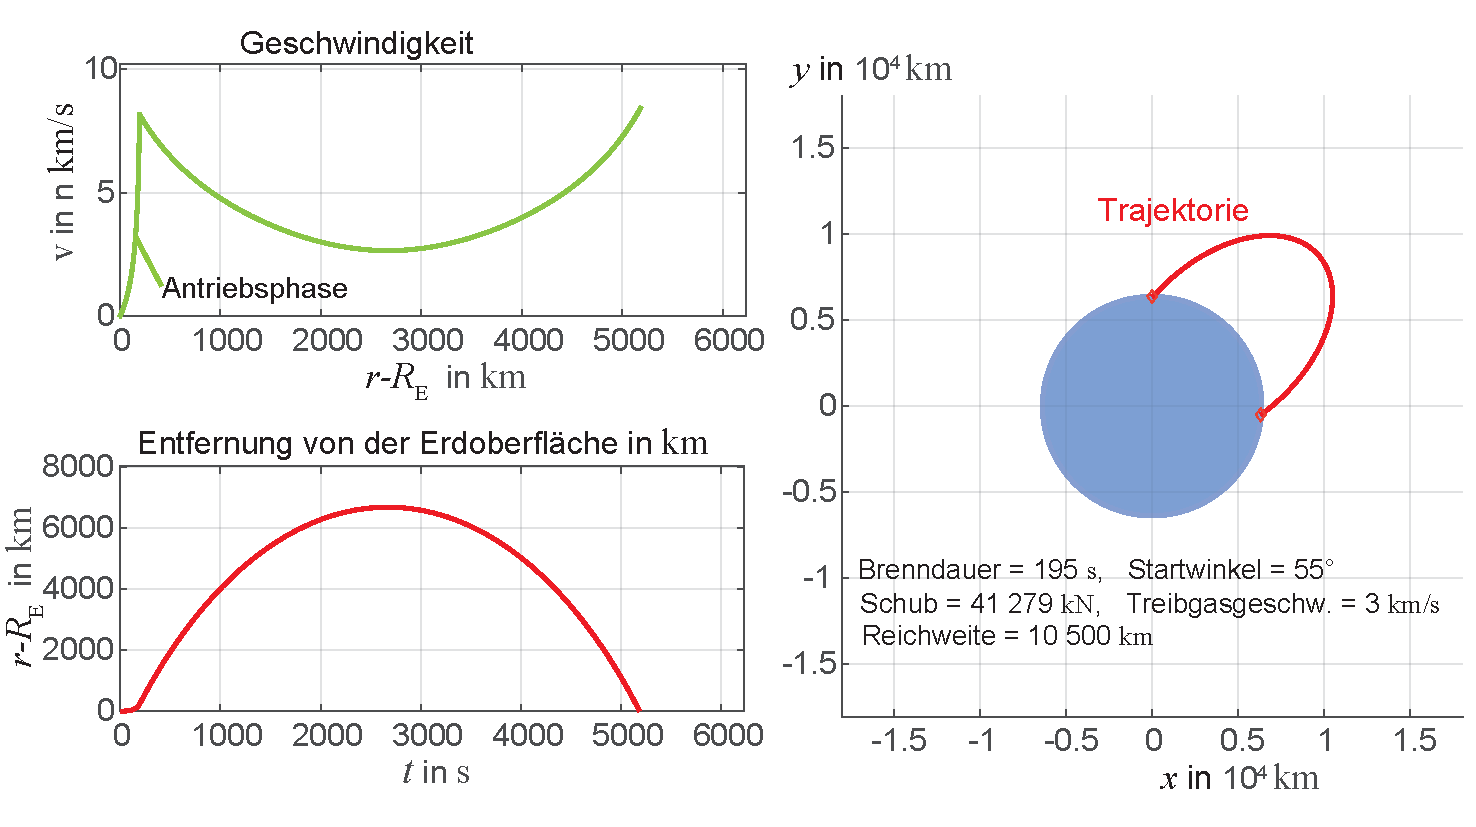
\includegraphics[width=\textwidth]{Rockets02.pdf} 
	\caption[Dynamik einer einstufigen von der Erdoberfl�che gestarteten Rakete.]{Numerische Berechnung der Dynamik einer einstufigen von der Erdoberfl�che gestarteten Rakete. Die numerische Rechnung (siehe \mscr\ \mladynref{Raketenstart01.m}) verwendete die vollst�ndige Bewegungsgleichung \eqref{eq:adyn_rockets01}, \dh ber�cksichtigt auch die Verringerung der Gravitationskraft in gr��eren H�hen, aber keine Reibung der Erdatmosph�re. Das werden wir in \kap{adyn_reentry} anschauen. Man erkennt, dass bei den gew�hlten Parametern die Rakete nach dem Brennschluss eine elliptische ballistische Bahn durchl�uft, die also keine volle Erdumrundung ergibt (adaptiert nach \cite{Hasbun2018})}.
	\label{abb:adyn_rockets02}
\end{figure}

\subsection{Nutzlast-�berlegungen}\index{Nutzlast}\index{Payload}\label{kap:adyn_payload}

\subsubsection{Wirkungsgrad}\label{kap:adyn_efficiency}

F�r das Design von Raketensystemen sind neben dem Schub \bzw dem erreichbaren Gesamtimpuls noch zwei �berlegungen wichtig. Zum einen der Wirkungsgrad und zum anderen die maximale Masse, die sich mit einer Rakete auf eine bestimmte Geschwindigkeit und damit auf eine bestimmte Bahn bringen l�sst. Wir wenden uns zun�chst dem Wirkungsgrad zu und betrachten den wichtigen inneren Wirkungsgrad. Dieser gibt an, wie viel Treibstoffenergie ben�tigt wird, um eine bestimmte Schubenergie zu erzeugen:
\begin{align}
    \eta_\text{int} = \frac{\frac{1}{2}{m_\text{T}\, v_\text{G}{}^2}}{E_\text{T}}  \label{eq:adyn_rockets08}\,.
\end{align}
Dieser Wirkungsgrad bestimmt, wie gro� $v_\text{G}$ und damit das Antriebsverm�gen $\Delta\, v$ bei einer bestimmten Treibstoffmenge $m_\text{T}$ (mit entsprechendem Energieinhalt $E_\text{T}$) letztendlich werden kann.

\subsubsection{Grenzen einstufiger Raketen}\label{kap:adyn_onestagerockets}

Wenn man sich Gleichung \eqref{eq:adyn_rocketequ} anschaut, k�nnte man auf die Vermutung kommen, dass man die Anfangsmasse (Startmasse) $m_1$ nur hinreichend gro� machen m�sste, um ein Raumschiff einer Masse $m_2$ auf eine beliebig gro�e Geschwindigkeit zu bringen. Dem ist aber nicht so. Wir betrachten dazu die Massenverh�ltnisse in einem Raketensystem genauer. Es gilt:
\begin{align}
\begin{split}
    t = t_0 : ~~ m_0 &= m_\text{S} + m_\text{L} + m_\text{T} \; , \\
		t = t_f : ~~ m_\text{f} &= m_\text{S} + m_\text{L} \;,
\end{split} \label{eq:adyn_rockets09}
\end{align}
worin $m_\text{S}$ die Masse der Struktur (Triebwerk, Schale \usw), $ m_\text{L}$ die Nutzlast (englisch \textit{Payload}) \glslink{payload} und $m_\text{T}$ die Treibstoffmasse jeweils zum Zeitpunkt $t=0$ sind.
Wir definieren das Nutzlastverh�ltnis\index{Nutzlastverh�ltnis} (englisch \textit{payload ratio}) mit
\begin{align}
    \mu_\text{L} = \frac{m_\text{L}}{m_0 - m_\text{L}} = \frac{m_\text{L}}{m_\text{S} + m_\text{T}} \label{eq:adyn_rockets10}\,
\end{align}
und das \gls{StrukturmassenVerhaeltnis} (englisch \textit{structural mass ratio}) \index{Strukturmassenverh�ltnis} durch:
\begin{align}
    \sigma_\text{S} = \frac{m_\text{S}}{m_0 - m_\text{L}} = \frac{m_\text{S}}{m_\text{S} + m_\text{T}} \label{eq:adyn_rockets11}\,.
\end{align}
Bildet man das Verh�ltnis von Endmasse zu Startmasse, so findet man �ber das Struktur\-massen-Verh�ltnis die Beziehung 
\begin{align}
    \frac{m_\text{f}}{m_0 } = \frac{\sigma_\text{S} + \mu_\text{L}}{1 + \mu_\text{L}} \label{eq:adyn_rockets12}\,.
\end{align}
Das Struktur\-massen-Verh�ltnis geht direkt in die L�sung der Ziolkowski-Gleichung ein und wir erhalten dann aus \eqref{eq:adyn_rocketequ}:
\begin{align}
\begin{split}
    \frac{\Delta v}{v_\text{G}} &= - \ln \frac{m_\text{f}}{m_0 } = - \ln \frac{\sigma_\text{S} + \mu_\text{L}}{1 + \mu_\text{L}} = \ln \frac{1 + \mu_\text{L}}{\sigma_\text{S} + \mu_\text{L}} ~~\text{\bzw} \\
		\mu_\text{L} &= \frac{\e^{-\Delta v/v_\text{G}}- \sigma_\text{S}}{1-\e^{-\Delta v/v_\text{G}}}\,. 
\end{split} \label{eq:adyn_rockets13}
\end{align}
Gl. \eqref{eq:adyn_rockets13} setzt das erzielbare Nutzlastverh�ltnis in Relation zu dem normierten Geschwindigkeitsgewinn $\Delta v/v_\text{G}$. Nun ist aber $v_\text{G}$ auf
\ca $\SI{4000}{\metre\per\second}$ begrenzt. Aus \figref{adyn_rockets03} kann man erkennen, dass zum Erreichen einer Endgeschwindigkeit von $\SI{8}{\km\per\second}$, selbst wenn man ein �u�erst optimistisches Struktur\-massen-Verh�ltnis von $\sigma_\text{S}=0.1$ annimmt, lediglich ein Nutzlastanteil von 3.5\%  realisiert werden kann. Gleichung \eqref{eq:adyn_rockets13} zeigt, warum gr��ere Nutzlasten \ia mit mehrstufigen Raketen ins All gebracht werden m�ssen. Dies werden wir im n�chsten Kapitel genauer untersuchen.

\begin{figure}
	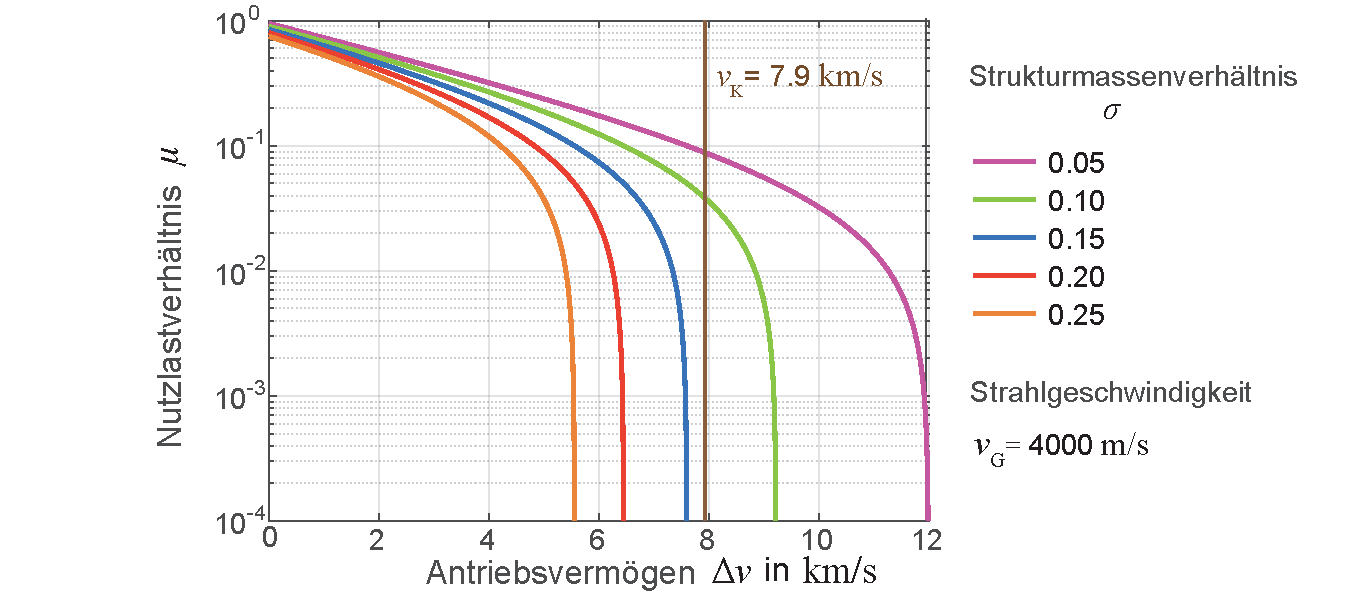
\includegraphics[width=\textwidth]{Rockets03.pdf} 
	\caption[Nutzlastverh�ltnis als Funktion der Endgeschwindigkeit $\Delta v$.]{Nutzlastverh�ltnis als Funktion der Endgeschwindigkeit $\Delta v$ bei angenommener Strahlgeschwindigkeit $v_\text{G} = \SI{4000}{\metre\per\second}$ nach Gleichung \eqref{eq:adyn_rockets13}. Die vertikale Linie zeigt die 1.~\gls{vkosmos}.}\index{Geschwindigkeit!1.~kosmische}
	\label{abb:adyn_rockets03}
\end{figure}

Zuvor aber noch eine Bemerkung zur charakteristischen Geschwindigkeit $\Delta v$. Im allgemeinen Fall wird man $\Delta v$ nur numerisch berechnen k�nnen, insbesondere bei l�nger andauernden Brennphasen des Triebwerks, wie wir das bei der numerischen Rechnung f�r \figref{adyn_rockets02} f�r den Aufstieg der Rakete im Gravitationsfeld der Erde getan haben. Wir hatten dort die anf�nglich noch stark wirkende Reibung der Atmosph�re unber�cksichtigt gelassen, werden dies aber sp�ter im \kap{adyn_launch_reentry} nachholen.\\
F�r die n�chsten Kapitel wollen wir den h�ufigen Fall eines zeitlich relativ kurzen Treibstoffaussto�es  voraussetzen. In diesem Fall k�nnen die wirkenden externen Kr�fte, insbesondere die Gravitationskraft $F_\text{G}$, als konstant angenommen werden und Gleichung \eqref{eq:adyn_rockets02} wird zu:
\begin{align}
     \Delta v &= - v_\text{G} \int_{m_0}^{m_\text{f}} \frac{\D m }{m} + F_\text{G} \int_{m_0}^{m_\text{f}} \frac{1}{\dot{m}} \frac{\D m}{m} = + \lk v_\text{G} - \frac{F_\text{G}}{\dot{m}_\text{T}} \rk\, \ln \frac{m_\text{f}}{m_0}		\,. \label{eq:adyn_rockets14}
\end{align}

\subsection{Prinzip der Stufenrakete}\label{kap:adyn_multistagerockets}

Wir haben im vorhergehenden Kapitel gesehen, dass mit einer einstufigen Rakete bei gegebenem Antriebsverm�gen die Nutzlast �u�erst begrenzt ist. Um gr��ere Nutzlasten ins Weltall zu bef�rdern, muss man das Prinzip der Stufenrakete \index{Stufenrakete} anwenden. Dieses besteht darin, dass w�hrend des Fluges unn�tig gewordene Strukturmassen der Rakete (leere Treibstoffbeh�lter, Triebwerke etc.) abgeworfen werden, um die verbleibende Antriebsenergie besser f�r die Beschleunigung der Nutzlasten zu verwenden. Man unterscheidet die Tandemstufung \index{Tandemstufung} (serielle Stufung) und die \index{Parallelstufung} Parallelstufung. Bei der ersteren erfolgt die Stufung �bereinander (\figref{adyn_rockets04}a), bei der Parallelstufung entsprechend parallel  (\figref{adyn_rockets04}b). H�ufig gibt es auch Mischformen \cite{Walter2018}. \\

\begin{figure}[H]
	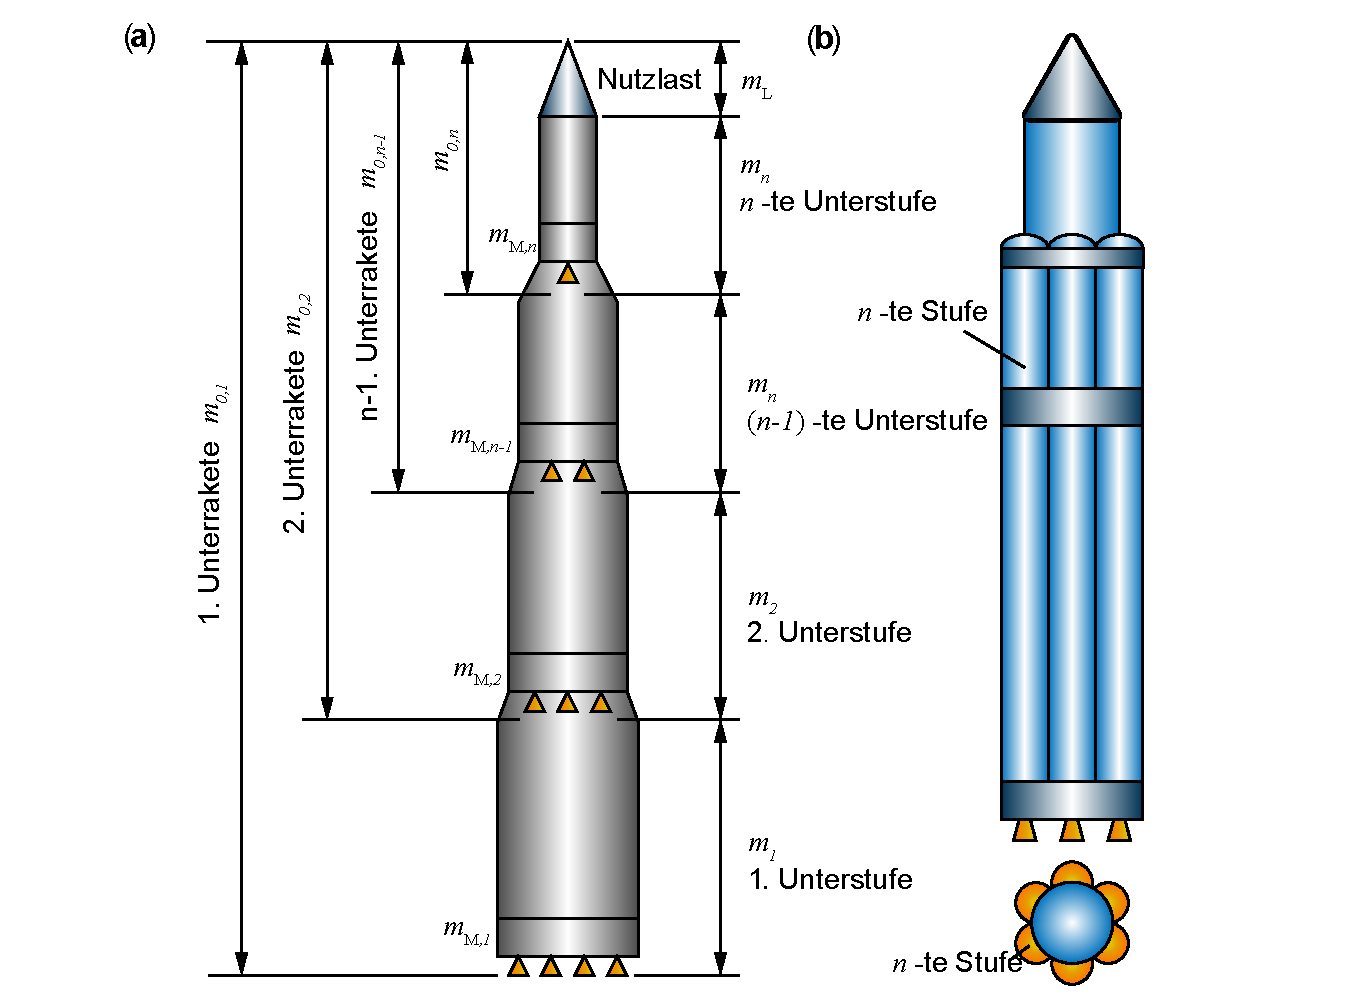
\includegraphics[width=\textwidth]{Mehrstufenraketen.pdf} 
	\caption[Mehrstufenprinzip bei Raketen.]{Mehrstufenprinzip bei Raketen. \fa Tandemstufung \fb Parallelstufung.}
	\label{abb:adyn_rockets04}
\end{figure}

Die Startmasse f�r eine $N$-stufige Rakete lautet:
\begin{align}
     m_0 &= \sum_{i=1}^N \, m_i + m_\text{L} \,, \label{eq:adyn_rockets15}
\end{align}
worin $m_\text{L}$ f�r die Nutzlast steht. Die Massen der einzelnen Stufen $m_i$ werden unterteilt in
\begin{align*}
     m_i &= m_{\text{T},i} + m_{\text{S},i}{} + m_{\text{M},i} \,.
\end{align*}
Hierin sind $m_{\text{T},i}$ die Massen des Treibstoffs, $ m_{\text{S},i}$ die Strukturmassen und $ m_{\text{M},i}$ die Triebwerksmassen der jeweils $i$-ten Stufe. Die Masse der Rakete nach Abbrennen und Abwerfen der $i$-ten Stufe ist gleichzeitig die Startmasse f�r die jeweilig n�chste Stufe, was die Definition von sogenannten Unterraketen mit den Massen $m_{0,i}$ erlaubt:
\begin{align}
\begin{split}
           m_{0,1} &= \lk \sum_{i=1}^N m_i \rk +  m_{\text{L}} = m_0 \,\\
		       m_{0,2} &= \lk \sum_{i=2}^N m_i \rk +  m_{\text{L}} \,\\
					         &\vdots \\
           m_{0,k} &= \lk \sum_{i=k}^N m_i \rk +  m_{\text{L}} \,\\
					         &\vdots \\
         m_{0,N+1} &= m_{\text{L}} = m_{\text{f}} \,.
\end{split} \label{eq:adyn_rockets16}
\end{align}


Mehrfache Anwendung der Raketen-Gleichung \eqref{eq:adyn_rocketequ} ergibt aus \eqref{eq:adyn_rockets16} f�r das Antriebsverm�gen\index{Antriebsverm�gen|textbf} $\Delta v$:
\begin{align}
     \Delta v &=  \sum_{i=1}^N v_{\text{G},i} \, \ln \frac{m_{0,i}}{m_{0,i}- m_{\text{T},i}} \,. \label{eq:adyn_rockets17}
\end{align}
Man beachte, dass im Nenner des Logarithmus von Gleichung \eqref{eq:adyn_rockets17} der Term $m_{0,i}- m_{\text{T},i}$ stehen muss, da zum Brenn-Endzeitpunkt der Stufe $i$ zwar der Treibstoff verbrannt ist, aber die Strukturen noch nicht abgeworfen worden sind. Man kann nun ein Strukturmassenverh�ltnis f�r die jeweiligen Stufen einf�hren:
\begin{align}
     \sigma_{\text{S},i} &= \frac{m_{0,i}- m_{\text{T},i} - m_{0,i+1}}{m_{0,i}} = \frac{m_{\text{M},i} + m_{\text{S},i}}{m_{0,i}}\,. \label{eq:adyn_rockets18}
\end{align}
Dieses kann man verstehen als das Verh�ltnis der momentanen (f�r $i$-te Stufe) eingesetzten Struktur- und Triebwerksmasse zur aktuellen Gesamtmasse, \dh der Masse der verbleibenden Unterrakete. Mit \eqref{eq:adyn_rockets18} folgt aus \eqref{eq:adyn_rockets17} f�r das gesamte Antriebsverm�gen:
\begin{align}
     \Delta v_\text{ges} &=  \sum_{i=1}^N v_{\text{G},i} \, \ln \frac{1}{\sigma_{\text{S},i} + m_{0,i+1}/m_{0,i}} = \sum_{i=1}^N v_{\text{G},i} \, \ln \frac{1}{\sigma_{\text{S},i} + \mu_{i+1}/\mu_i}  \,,\label{eq:adyn_rockets19}
\end{align}
wobei wir als 
\begin{align}
	\mu_i = m_{0,i}/m_0  \label{eq:adyn_rockets19a}
\end{align}
das Massenverh�ltnis der $i$-ten Unterrakete zur Gesamtstartmasse eingef�hrt haben, womit insbesondere gilt:
\begin{align}
		\mu_1 = 1\,,~~\mu_{N+1} = m_\text{L}/m_0 = \mu_\text{L}\,. \label{eq:adyn_rockets19b}
\end{align}
Wir sehen an Gleichung \eqref{eq:adyn_rockets19}, dass f�r das Antriebsverm�gen der Rakete die Struktur\-massen-Verh�ltnisse und die relativen Massenverh�ltnisse entscheidend sind. Man kann leicht �berpr�fen, dass \eqref{eq:adyn_rockets19} f�r $N=1$ in die Ziolkowski-Gleichung\index{Ziolkowski-Gleichung} �bergeht. Offensichtlich stellt \eqref{eq:adyn_rockets19} eine komplexe Optimierungsaufgabe f�r die Bestimmung des mehrstufigen Raketensystems bei vorgegebener Nutzlast $m_\text{L}$  und Maximierung \bzw Erreichung eines bestimmten Antriebsverm�gens $\Delta v_\text{ges}$ dar. 
Die Stufenoptimierungsaufgabe besteht insbesondere darin,  die Zahl der Stufen $N$ und die Massenaufteilung $m_{0,i}$ auf die einzelnen Raketenstufen so festzulegen, dass die Gesamtmasse  $m_0$ minimal wird. 
Vorgegeben sind dabei die Gasaustrittsgeschwindigkeiten $v_{\text{G},i}$ der einzelnen Stufen. Ebenso werden die Strukturmassenverh�ltnisse $\sigma_{\text{S},i}$ der einzelnen Stufen, die von der Beschleunigungsbelastung, der G�te der Konstruktion, der Bauweise und vielen anderen Faktoren abh�ngen, als bekannte Konstanten vorausgesetzt. Siehe dazu auch \probref{adyn_rocketbasic} und \probref{adyn_rocketopt2}, die Optimierungsaufgabe werden wir speziell in \probref{adyn_rocketopt1} durchf�hren.
In \figref{adyn_rockets05} haben wir das Nutzlastverh�ltnis und das Antriebsverm�gen mit den Werten der Saturn V und der Ariane 1 Raketen aufgetragen \cite{Messerschmid2017}. Man erkennt, dass mit h�herer Stufenzahl das Antriebsverm�gen wie erwartet zunimmt. 

\begin{figure}[H]
	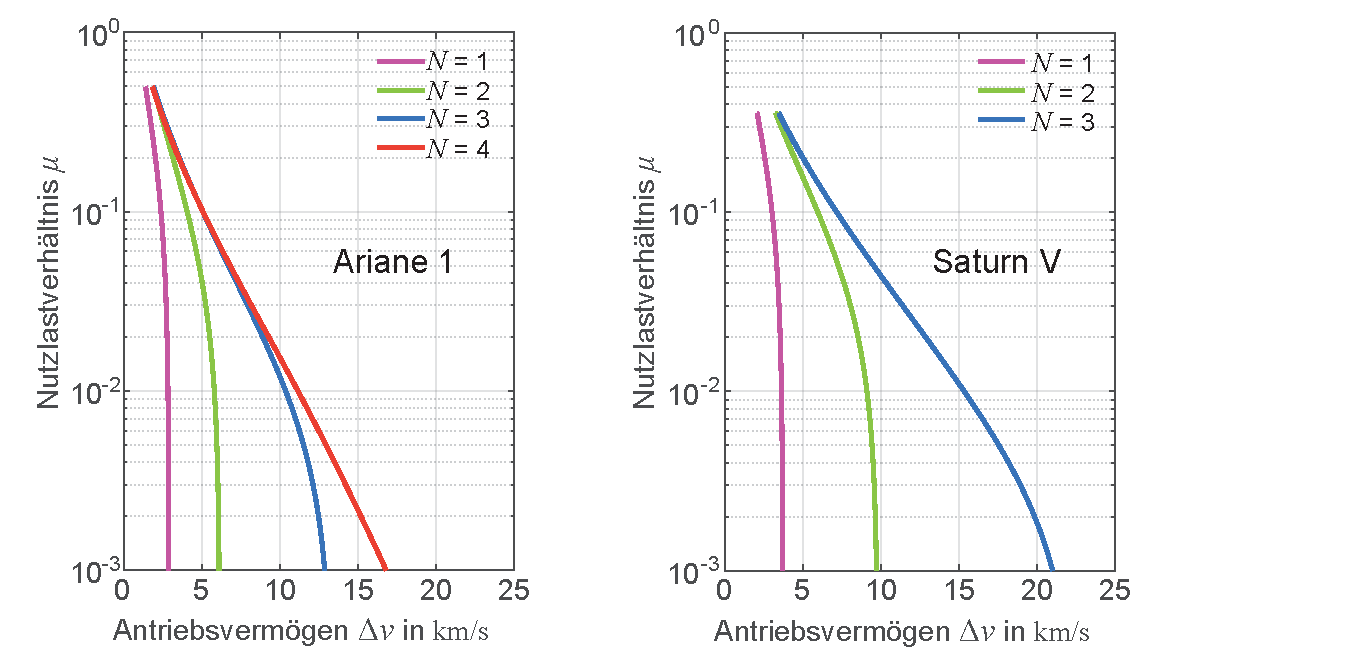
\includegraphics[width=\textwidth]{ArianeSaturn.pdf} 
	\caption[Nutzlastverh�ltnis f�r mehrstufige Raketen.]{Nutzlastverh�ltnis f�r mehrstufige Raketen (Werte f�r Saturn~V und der Ariane~1 siehe Tabelle \ref{tab:adyn_parameter_raketen} \cite{Messerschmid2017}).}
	\label{abb:adyn_rockets05}
\end{figure}





\section{Umlaufbahnen von k�nstlichen Himmelsk�rpern}\label{kap:adyn_orbits}

Im vorherigen Kapitel hatten wir die Geschwindigkeits�nderung eines Raumflugk�rpers unter Wirkung eines Schubs betrachtet. Wenn dieser Schub nur f�r kurze Zeit wirkt, k�nnen w�hrend dieser Phase dann alle anderen wirkenden Kr�fte und auch die Positions�nderung des Raumschiffs \bzw der Rakete unber�cksichtigt bleiben und man muss nur die Geschwindigkeits�nderung $\Delta v$ betrachten. Wirkt der Schub hingegen �ber eine l�ngere Zeit, dann muss man die Bewegungsgleichung \eqref{eq:adyn_rockets01} unter Ber�cksichtigung aller wirkenden Kr�fte entsprechend integrieren (wie zum Beispiel in der Rechnung zu \figref{adyn_rockets02}). 
Im Folgenden nehmen wir die Wechselwirkungszeit des Schubs zun�chst als sehr kurz an, in \kap{adyn_kont_maneuver} werden wir auch Phasen betrachten, in denen der Schub �ber eine l�ngere Zeit wirkt.\\
In den Flugphasen ohne Schub bewegt sich das Raumschiff im Gravitationsfeld der Himmelsk�rper nach den Gesetzen der Himmelsmechanik, im einfachsten Fall auf Kepler-Bahnen des Zweik�rpersystems Himmelsk�rper-k�nstlicher Satellit. Wir wollen daher zun�chst den Fall von Satellitenbahnen um die Erde betrachten und stellen daf�r noch einmal die im Kapitel der Himmelsmechanik (Kap. \ref{chap:hm}) hergeleiteten wichtigsten Beziehungen f�r das Zweik�rperproblem, angepasst f�r (geschlossene) Satellitenbahnen um die Erde, zusammen.

\subsection{Grundlegende Beziehungen aus der Himmelsmechanik f�r Satellitenbahnen um die Erde}\label{kap:adyn_recap_hm}

F�r k�nstliche Satelliten der Masse $m$ um die Erde gilt: 
\begin{align}
    m \ll m_\text{E} ~~~~ \rightarrow ~~~~ \mu_\text{G} = G\,m_\text{E}\,.  \label{eq:adyn_orbit01}
\end{align}
Aus den im \kap{hm_abl_kepler} hergeleiteten Beziehungen f�r die Ellipsenbahn folgt dann mit dem Drehimpuls $L$ f�r die Bahnparameter $p, a, e ~\text{und}~ T_\text{P}$ und den Koordinaten $r, v$:
\begin{subequations}
\begin{align}
    r &= \frac{p}{1+\e \cos\upsilon} ~~~\text{mit}\\
    p &=\frac{L^2}{G\,m_\text{E}}\,,~~~ e = \sqrt{1-\frac{L^2}{a\,m_\text{E}}}~~~\text{und}~~~ a= \sqrt[3]{\frac{G\,m_\text{E}\,T_\text{P}{}^2}{4\pi^2}}\,.
		\label{eq:adyn_orbit01a} 
\end{align}
\end{subequations}
F�r das \gls{perigee}\index{Perig�um|textbf} \bzw das \gls{apogee}\index{Apog�um|textbf} gilt dann: 
\begin{align}
    r_\text{min} &= r_\text{per} = \frac{p}{1+e} ~~~ \text{und}~~~  r_\text{max} = r_\text{apo} = \frac{p}{1-e} \,. \label{eq:adyn_orbit01b} 
\end{align}

\begin{figure}[H]
	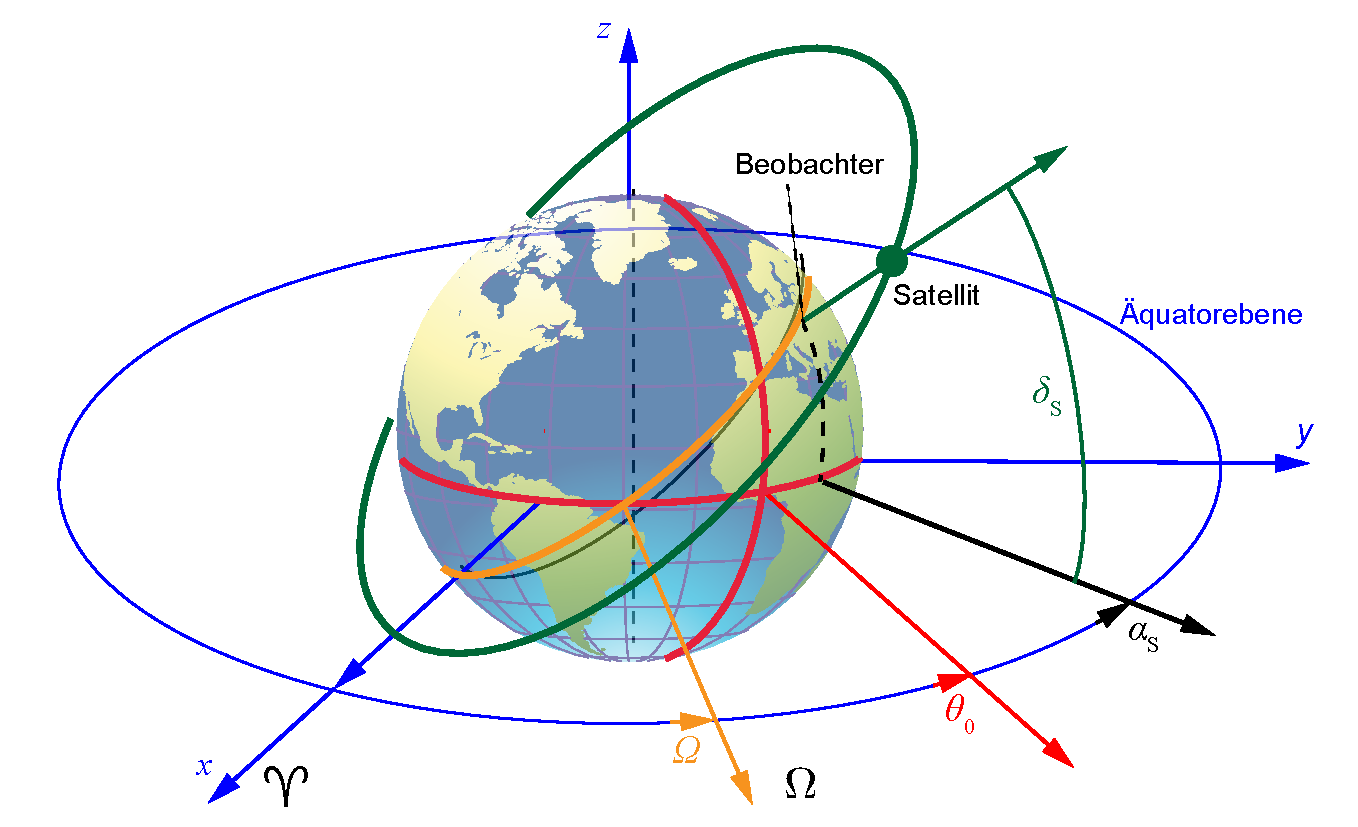
\includegraphics[width=\textwidth]{Orbits01.pdf} 
	\caption[Bahnparameter und Koordinatensystem einer Satellitenbahn um die Erde.]{Bahnparameter und Koordinatensystem einer Satellitenbahn um die Erde. Die Winkel $\Omega,\, \theta_0,\, \alpha_\text{S}$ werden jeweils vom Fr�hlingspunkt\index{Fr�hlingspunkt} aus gemessen.}
	\label{abb:adyn_orbits01}
\end{figure}

Die \gls{visvivaadyn} \eqref{eq:hm_vis-viva} lautet
\begin{align}
    v^2 = G\,m_\text{E} \lk \frac{2}{r} -\frac{1}{a}\rk \,, \label{eq:adyn_orbit03}
\end{align}
woraus sich die Geschwindigkeiten am Perig�um \bzw Apog�um ergeben:
\begin{subequations}
\begin{align}
    v_\text{max} &= v (r_\text{min}) = v_\text{per} = \sqrt{\frac{G\,m_\text{E}}{a}}\,\sqrt{\frac{1+\e}{1-\e}} ~~~ \text{\bzw} \\
		v_\text{min} &= v (r_\text{max}) = v_\text{apo} = \sqrt{\frac{G\,m_\text{E}}{a}}\,\sqrt{\frac{1-\e}{1+\e}}\,.
\end{align} \label{eq:adyn_orbit04}
\end{subequations}

Die Bahnparameter $\Omega,\omega,i$ (\figref{adyn_orbits01}) entsprechen den Bahnparametern, wie sie f�r Planeten und andere nat�rliche Himmelsk�rper in \kap{hm_bewegungsgl} hergeleitet (\figref{hm_bahnelemente}) wurden. \\
Entsprechend kann man die Bewegung eines k�nstlichen Satelliten au�erhalb der Schubphasen durch die in \kap{hm_bahnen_hk_ss} hergeleiteten Gau�schen
%\footnote{Johann Carl Friedrich Gau� (auch oft Gauss) (1777 -- 1855) war ein deutscher Mathematiker, Astronom, Geod�t und Physiker. Wegen seiner �berragenden wissenschaftlichen Leistungen galt er bereits zu seinen Lebzeiten als \textit{Princeps mathematicorum - F�rst der Mathematiker}. Seine Arbeiten erstreckten sich von vielen Feldern der Mathematik und Physik auch auf angewandte Gebiete, zum Beispiel der Landesvermessung und der elektromagnetischen Telegrafie.}\indexp{Gau�, Johann Carl Friedrich} 
 Vektoren\footnote{In \kap{hm_bahnen_hk_ss} hatten wir der historischen Konvention folgend die Gau�schen Vektoren mit $\vec{P}\vec{Q}\vec{R}$  bezeichnet. Um Verwechslungen mit dem Radiusvektor $\vec{R}$ zu vermeiden, schreiben wir ab hier $\vec{R}=\vec{W}$.}  \eqref{eq:hm_gauss_ansatz},\eqref{eq:hm_gauss_vektoren} $\vec{P}\vec{Q}\vec{W}$ beschreiben:
\begin{align}
\begin{split}
    \vec{r}_\text{S} &= 
    \begin{pmatrix}
        x_\text{S} \\
        y_\text{S} \\
        z_\text{S}
    \end{pmatrix}
    = \mathbb{U}\,r\,    
		\begin{pmatrix}
        \cos\upsilon \\
        \sin\upsilon \\
        0
    \end{pmatrix}
		= 
    \lk \vec{P}\vec{Q}\vec{W}\rk\,\,r\,
    \begin{pmatrix}
        \cos\upsilon \\
        \sin\upsilon \\
        0
    \end{pmatrix} \\
    &= \mathbb{R}_z\lk -\Omega\rk\,\mathbb{R}_x\lk -i\rk\,\mathbb{R}_z\lk -\omega\rk\,\,r\,
    \begin{pmatrix}
        \cos\upsilon \\
        \sin\upsilon \\
        0
    \end{pmatrix} \,,
\end{split} \label{eq:adyn_orbit05}
\end{align}\\
wobei sich die wahre Anomalie\index{Anomalie!wahre} $\upsilon$ aus der Kepler-Gleichung \eqref{eq:hm_keplerglg} �ber die exzentrische Anomalie $E$\index{Anomalie!exzentrische} berechnen l�sst.
Wie man aus \figref{adyn_orbits01} sieht, ist die Satellitenbahnebene ein Gro�kreis, der eindeutig durch die Bahnneigung (Inklination) $i$ und den aufsteigenden Knoten festgelegt ist. Dieser Gro�kreis schneidet somit die �quatorebene unter dem Winkel~$i$. Die maximale (minimale) geographische Breite, unter der der Satellit beobachtet werden kann, ist dann durch $+\,i$ \bzw $-\,i$ gegeben, wie man ebenfalls aus \figref{adyn_orbits01} sieht.

\subsection{Bestimmung der Bodenspuren k�nstlicher Satelliten} \label{kap:adyn_orbits_groundtracks}

Wir nehmen zun�chst an, dass uns die Bahnparameter des Satelliten bekannt sind, wir also seine geozentrische Bahn berechnen k�nnen, so wie wir das f�r Planeten als nat�rliche Satelliten der Sonne im \kap{hm_bahnen_hk_ss} ausf�hrlich beschrieben haben. Wir wollen jetzt aber auch die Projektion dieser Bahn auf die Erdoberfl�che berechnen. Dazu brauchen wir zu jeder Zeit den geographischen Ort, �ber dem der Satellit senkrecht steht. Die jeweilige geographische Breite $\varphi_\text{B}$ des Ortes B (eigentlich die geozentrische Breite), �ber welchem der Satellit im Zenit steht, ist durch die Deklination des Satelliten $\delta_\text{S}(t)$ gegeben, die sich wiederum aus \eqref{eq:adyn_orbit05} berechnen l�sst. Die entsprechende geographische L�nge $\lambda_\text{B}$ h�ngt, wie im \kap{hm_zeitdefinition}, \figref{hm_Sternzeit_Stundenwinkel} gezeigt, von der Rektaszension $\alpha_\text{S}\lk t\rk$ des Satelliten ab (vgl. \eqref{eq:hm_std_winkel_tau}), woraus sich mit \eqref{eq:hm_UT_3} die folgende Beziehung ergibt \cite{Montenbruck2012}:
\begin{align}
    \lambda_\text{B}\lk t\rk = \alpha_\text{S}\lk t\rk -\theta_0 = \alpha_\text{S}\lk t\rk + 280.4606\degree + 360.9856473\degree d \,. \label{eq:adyn_orbit06}
\end{align}
Hierin ist $\theta_0$ die (mittlere) Greenwich Sternzeit (GMST) und $d$ ist die seit dem $1.1.2000$ verstrichene Zeit in (Julianischen) Tagen, die sich einfach aus $d = \mathrm{MJD} - 51544.5$ berechnen l�sst. Sinnvollerweise benutzt man das (modifizierte) Julianische Datum MJD ebenfalls zur Berechnung von $\alpha_\text{S}(t)$ und $\delta_\text{S}(t)$ (\vgl \kap{hm_zeitdefinition}). Als Ergebnis der �ber die Beziehung \eqref{eq:adyn_orbit06} ber�cksichtigten Erdrotation relativ zur Bewegung des Satelliten ist der Pfad des Satelliten auf der Erdoberfl�che kein einfacher Gro�kreis mehr, sondern hat \zb f�r einen sogenannten \gls{LEO}\index{Low Earth Orbit, LEO} die in \figref{adyn_orbits02} dargestellte Form. Offensichtlich sind die Bodenspuren f�r aufeinanderfolgende Orbits wegen der Erdrotation jeweils westlich verschoben.
F�r einen Satelliten mit einer ann�hernd kreisf�rmigen Bahn und einer Umlaufzeit von $T_\text{p}$ in Minuten verschiebt sich die geographische L�nge eines Beobachtungspunktes auf dem �quator um 
\begin{align*}
    \Delta \lambda_\text{B,�q} = -\dot{\theta}_0\,T_\text{p} = -0.2507\degree\,T_\text{p}
\end{align*}
pro Umlauf (\figref{adyn_orbits02}). \\
F�r andere Satellitenbahnen, wie \zb geostation�re Bahnen (\gls{GEO}, GEO)\index{Orbit!geostation�rer, GEO} oder hoch elliptische Bahnen (\gls{HEO}, HEO)\index{Orbit!highly elliptical, HEO} ergeben sich deutlich andere Bodenspuren (siehe \figref{adyn_orbits03} und \probref{adyn_orbits2}).

\begin{figure}[H]
	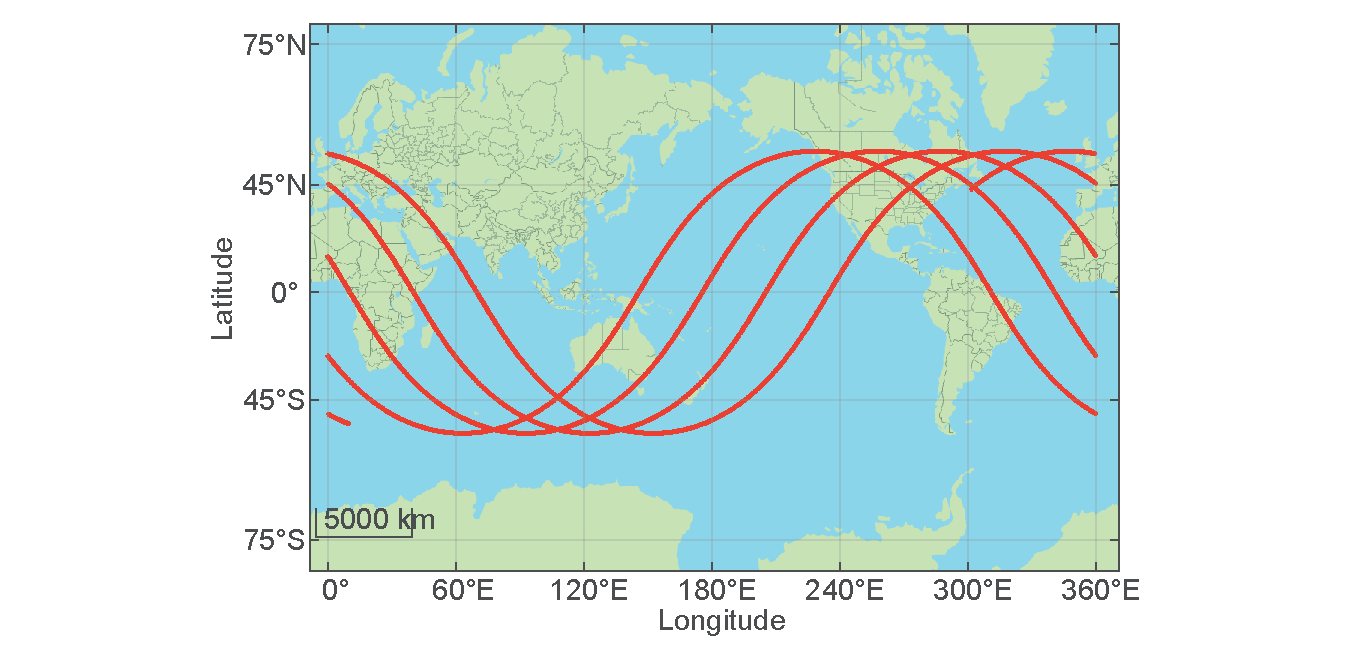
\includegraphics[width=\textwidth]{Orbits02.pdf} 
	\caption[Bodenspur eines LEO-Satelliten.]{Bodenspur eines LEO-Satelliten. $a = \SI{8000}{\km},\; e = 0.0,\; i = 55\degree$.}
	\label{abb:adyn_orbits02}
\end{figure}

\begin{figure}[H]
	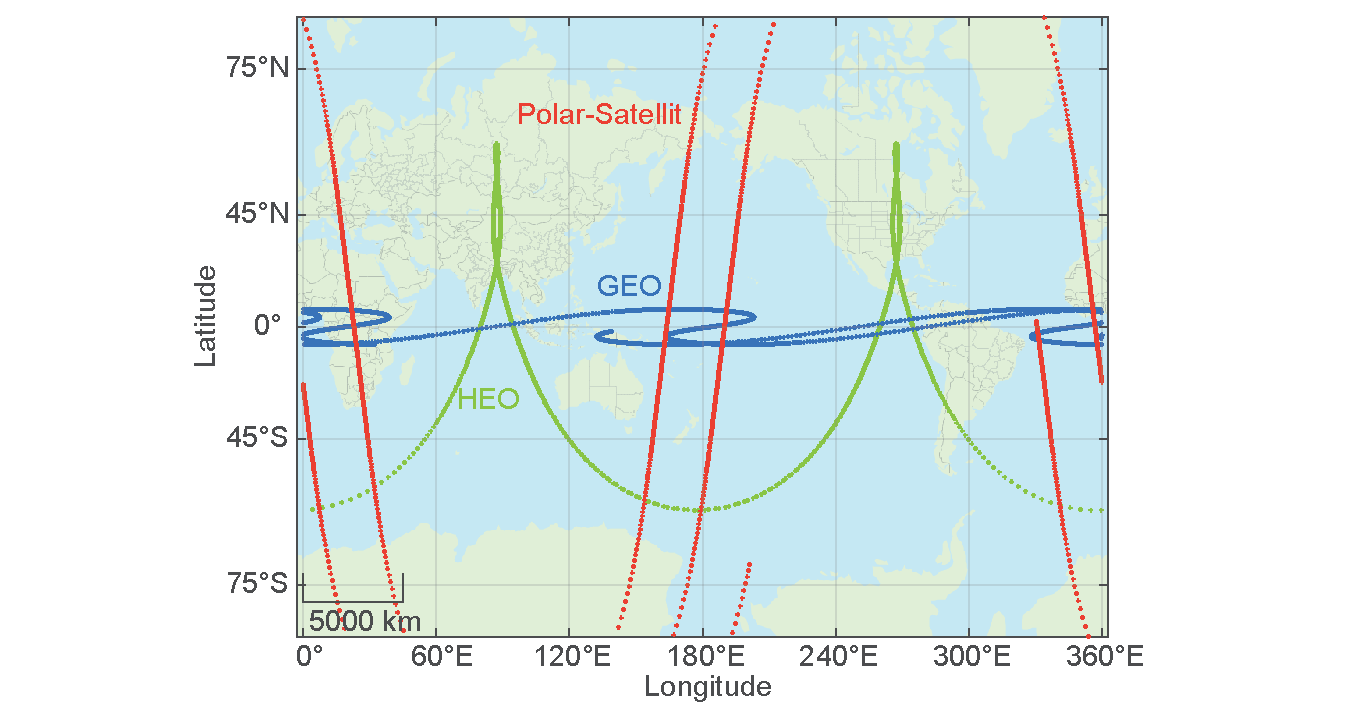
\includegraphics[width=0.9\textwidth]{Orbits03a.pdf} 
	\caption[Bodenspuren von verschiedenen Satelliten.]{Bodenspuren von verschiedenen Satelliten. GEO-artiger Satellit:\, $a = \SI{25000}{\km},\, e = 0.73,\, i = 8\degree,\, \Omega =45\degree$,\,\, HEO (Typ Molnija-Satelliten):\, $a = \SI{26555}{\km},\, e = 0.72,\, i = 63.4\degree,\, \Omega =120\degree,\,\omega =270\degree$,\,\, Polar-Satellit:\, $a = \SI{7330}{\km},\, e = 0.0,\, i = 93\degree,\, \Omega =130\degree,\,\omega =0\degree$. Siehe auch \mscr~ \mladynref{SatPositionen01.m}.}
	\label{abb:adyn_orbits03}
\end{figure}

\subsection{Topographische Beziehungen f�r die Beobachtungen k�nstlicher Satelliten} \label{kap:adyn_orbits_topo}

Will man die Beobachtungsdaten eines in der Erdumlaufbahn befindlichen Satelliten f�r eine bestimmte Bodenstation aus den Bahnparametern berechnen, so muss man, wie bereits im Kapitel Himmelsmechanik (\kap{hm_koordinatensysteme}) gezeigt, in ein topozentrisches Koordinatensystem wechseln, da ein Beobachter auf der Erdoberfl�che einen Satelliten aus der Horizont\-ebene (\figref{adyn_satobserv01}) beobachten wird. Die Bodenspuren (englisch \textit{Ground-Tracks}) aus dem vorherigen Kapitel geben eine gewisse Indikation, aber man erh�lt daraus keine Aussage �ber die H�he des Satelliten, die Sichtbarkeitsdauer und auch die Beobachtungsrichtung. Um diese Gr��en zu berechnen, gehen wir in ein lokales tangentiales Koordinatensystem, welches ein spezielles topozentrisches \KOS\ darstellt (\figref{adyn_satobserv01}, \vgl auch \kap{hm_koordinatensysteme}). Wir wollen nun die Position des Satelliten in diesem Koordinatensystem ausdr�cken. \\

\begin{figure}[H]
	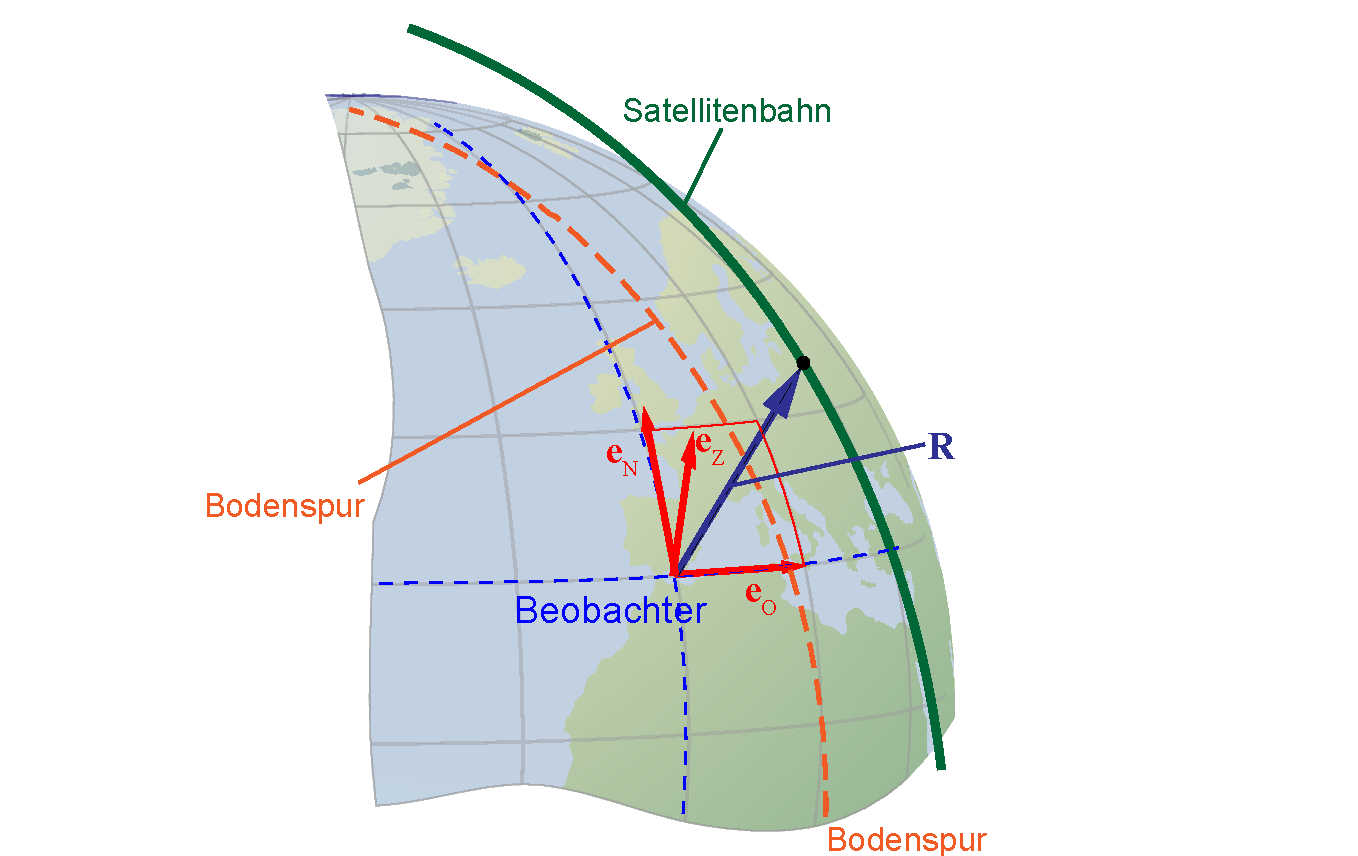
\includegraphics[width=\textwidth]{SatObserver01.pdf} 
	\caption[Horizontkoordinatensystem.]{Horizontkoordinatensystem und beobachtbarer Anteil der Umlaufbahn eines Satelliten.}
	\label{abb:adyn_satobserv01}
\end{figure}

Wir starten mit den Koordinaten des Satelliten $\vec{r}$ im geozentrisch-�quatorialen Koordinatensystem und schreiben diese als $\vec{r}_\text{S}$ in ein erdfestes geozentrisch-�quatorialen System  um, in dem wir die Rotation der Erde durch den Stundenwinkel von Greenwich $\theta$ ber�cksichtigen (vgl. \kap{hm_koordinatensysteme}, Gleichung \eqref{eq:hm_LMST}, \figref{hm_Sternzeit_Stundenwinkel}):
\begin{align}
\begin{split}
    \vec{r}_\text{S} &= \mathbb{R}_\text{z}\!\lk\theta\rk\,\vec{r}\, ~~~~
\text{mit} ~~~~ \mathbb{R}_\text{z}\lk\theta\rk = 
    \begin{pmatrix}
         \cos\theta & ~~\sin\theta & ~~0 \\
        -\sin\theta & ~~\cos\theta & ~~0 \\
        0             & ~~0            &~~ 1
    \end{pmatrix} \\
		\text{und}~~~~\theta &= 280.4606\degree + 360.9856473\degree \cdot \lk \mathrm{MJD} - 51544.5\rk \,,
\end{split} \label{eq:adyn_statobserv01} 
\end{align}
worin MJD das modifizierte Julianischem Datum (Kap. \ref{kap:hm_zeitdefinition}) des Beobachtungszeitpunkts ist. Die Koordinaten des Beobachters sind gegeben durch:
\begin{align}
    \vec{r}_\text{B} = R_\text{E}
    \begin{pmatrix}
		                     \cos \varphi_\text{B} \, \cos \lambda_\text{B} \\
		                     \cos \varphi_\text{B} \, \sin \lambda_\text{B} \\
		                     \sin \varphi_\text{B}
    \end{pmatrix} \,, \label{eq:adyn_statobserv02}
\end{align} 
wobei wir f�r die geographische Breite \bzw L�nge verk�rzend $\varphi=\varphi_\text{B}$ \bzw $\lambda= \lambda_\text{B}$ schreiben.\footnote{Wie bereits erw�hnt, setzen wir die geographische Breite hier gleich der geozentrischen Breite, \dh wir vernachl�ssigen die Abplattung der Erde.} Der topozentrische, fest mit der Erde verbundene Koordinatenvektor $\vec{R}_\text{S}$ ist in �quatorialen Koordinaten dann durch 
\begin{align}
\begin{split}
    \vec{R}_\text{S} &= \vec{r}_\text{S} - \vec{r}_\text{B}\,
\end{split} \label{eq:adyn_statobserv03} 
\end{align}
bestimmt.\\
Die Einheitsvektoren des topozentrischen \KOS\ lauten:
\begin{align}
\begin{split}
    \vec{e}_\text{O} &= 
    \begin{pmatrix}
        -\sin\lambda_\text{B}\\
        +\cos\lambda_\text{B}\\
        0
    \end{pmatrix} ~~~ \text{(Ost-Richtung)}\,,~~~
    \vec{e}_\text{N} = 
    \begin{pmatrix}
        -\sin\varphi_\text{B}\cos\lambda_\text{B}\\
        -\sin\varphi_\text{B}\sin\lambda_\text{B}\\
        \cos\varphi_\text{B}
    \end{pmatrix} ~~~ \text{(Nord-Richtung)}\,,\\
    \vec{e}_\text{Z} &= 
    \begin{pmatrix}
        \cos\varphi_\text{B}\cos\lambda_\text{B}\\
        \cos\varphi_\text{B}\sin\lambda_\text{B}\\
        \sin\varphi_\text{B}
    \end{pmatrix} ~~~ \text{(Zenit-Richtung)}\,.
\end{split} \label{eq:adyn_statobserv04} 
\end{align}
F�r die Umrechnung von erdfesten �quatorialen in topozentrische Koordinaten verwendet man die Transformationsmatrix $\mathbb{U}$, die durch die drei Einheitsvektoren nach \eqref{eq:adyn_statobserv04}  definiert wird:
\begin{align}
    \mathbb{U}= 
		\begin{pmatrix}
        \vec{e}_\text{O}{}^\text{T} \\
        \vec{e}_\text{N}{}^\text{T} \\
        \vec{e}_\text{Z}{}^\text{T} 
    \end{pmatrix} =
    \begin{pmatrix}
        -\sin\lambda_\text{B} &~~ +\cos\lambda_\text{B} &~~ 0 \\
        -\sin\varphi_\text{B}\,\cos\lambda_\text{B} &~~ -\sin\varphi_\text{B}\,\sin\lambda_\text{B}&~~\cos\varphi_\text{B}\\
        +\cos\varphi_\text{B}\,\cos\lambda_\text{B} &~~ +\cos\varphi_\text{B}\,\sin\lambda_\text{B}&~~ \sin\varphi_\text{B}
    \end{pmatrix} \,. \label{eq:adyn_statobserv05} 
\end{align}
Wir erhalten damit leicht den Beobachtungsvektor zum Satelliten $\vec{R}$ in kartesischen topozentrischen Koordinaten:% (Distanz $R$, Azimut $\mathcal{A}$ und H�he $h$)
\begin{align}
    \vec{R} = 
    \begin{pmatrix}
        R_\text{O} \\
        R_\text{N}\\
        R_\text{Z}
    \end{pmatrix}
    &= \mathbb{U}\,\vec{R}_\text{S} =
    \mathbb{U}\,\lek \lk \mathbb{R}_\text{z}\lk \theta\rk \,\vec{r} \rk - \vec{r}_\text{B} \rek \,.
\end{align} \label{eq:adyn_statobserv06}
Die Beobachtungsdaten Azimut $\mathcal{A}$ und H�he $h$ sind dann leicht zu bestimmen:
\begin{align}
    \mathcal{A} &= \arctan\lk \frac{R_\text{O}}{R_\text{N}}\rk ~~~\text{und}~~~
    h = \arctan\lk \frac{R_\text{Z}}{\sqrt{R_\text{O}{}^2 + R_\text{N}{}^2}}\rk \,.\label{eq:adyn_statobserv07}
\end{align}
Wie aus \figref{adyn_satobserv01} ableitbar, beschreibt $\mathcal{A}$ den Winkel zwischen der Bodenspur des Satelliten und der Nordrichtung und $h$ den Winkel zwischen der Richtung von Beobachter zum Satelliten und der Horizontebene. In \probref{adyn_orbits3} werden wir die Beobachtungsdaten f�r einen polaren Satelliten und die ISS berechnen. %�bung7

\subsection{Bestimmung der Bahn k�nstlicher Satelliten vom Boden aus} \label{kap:adyn_orbits_determination}

\subsubsection{Bestimmung der Bahn k�nstlicher Satelliten aus Orts- und Geschwindigkeitsmessungen vom Boden} \label{kap:adyn_orbits_determination_rv}

Wir nehmen an, dass zu einem Zeitpunkt $t$ die geozentrischen Orts- \bzw Geschwindigkeitsvektoren ($\vec{r}, \vec{v}=\dot{\vec{r}}$) des Satelliten gegeben sind.\\
Der spezifische Drehimpuls $\vec{L} = \vec{r} \times \dot{\vec{r}} = \begin{pmatrix}
    y\,\dot{z} - z\,\dot{y}\\
    z\,\dot{x} - x\,\dot{z}\\
    x\,\dot{y} - y\,\dot{x}
\end{pmatrix}$ ist mit dem Gau�-Vektor\index{Gau�-Vektor|textbf} $\vec{W}$ wie folgt verkn�pft:
\begin{align}
    \begin{pmatrix}
        \sin i \,\sin\Omega\\
        \sin i \,\cos\Omega\\
        \cos i
    \end{pmatrix}
    = 
    \begin{pmatrix}
        +L_x/L\\
        -L_y/L\\
        +L_z/L
    \end{pmatrix}
    = 
    \begin{pmatrix}
        +W_x\\
        -W_y\\
        +W_z
    \end{pmatrix} \,. \label{eq:adyn_Bahnpara01}
\end{align}
Daraus erh�lt man sofort
\begin{align}
    i = \arctan\lk\frac{\sqrt{W_x{}^2+W_y{}^2}}{W_z}\rk \label{eq:adyn_Bahnpara02}
\end{align}
und 
\begin{align}
    \Omega = \arctan\lk\frac{W_x}{-W_y}\rk \label{eq:adyn_Bahnpara03}\,.
\end{align}
Der Drehimpuls ist nach \eqref{eq:hm_kegelschnitt} \bzw  \eqref{eq:adyn_orbit01a} mit dem Parameter $p$ �ber 
\begin{align}
    p = \frac{L^2}{G\,m_\text{E}} \label{eq:adyn_Bahnpara04}
\end{align}
verkn�pft. Der \textit{vis-viva-Satz}\index{vis-viva-Satz} \eqref{eq:hm_vis-viva} \bzw \eqref{eq:adyn_orbit03} ergibt aus den Messwerten sofort die gro�e Halbachse $a$ und die mittlere Bewegung\index{Bewegung!mittlere} $n$ �ber:
\begin{align}
    a = \lk \frac{2}{r} - \frac{v^2}{G\,m_\text{E}} \rk^{-1}~~~\text{\bzw}~~~ n = \sqrt{\frac{G\,m_\text{E}}{a^3}} \,, \label{eq:adyn_Bahnpara05}
\end{align}
und damit erhalten wir auch die Exzentrizit�t $e$: 
\begin{align}
    e = \sqrt{1-\frac{p}{a}} \,.\label{eq:adyn_Bahnpara07}
\end{align}
�ber die exzentrische Anomalie 
\begin{align}
    E\lk t\rk = \arctan\lk\frac{\vec{r}\cdot\vec{v}/(a^2\,n)}{1-r/a}\rk \label{eq:adyn_Bahnpara08}
\end{align}
und die Kepler-Gleichung erh�lt man die mittlere Anomalie zum Zeitpunkt $t$:
\begin{align}
    M\lk t\rk =E\lk t \rk - e\,\sin E\lk t\rk \label{eq:adyn_Bahnpara09}\,.
\end{align}
Etwas aufwendiger ist die Berechnung des Arguments des Perig�ums. \\
Man muss zun�chst die L�nge $u$ berechnen,
\begin{align}
    u = \arctan\lk\frac{z/\sin i }{x\,\cos\Omega +y\,\sin\Omega}\rk\,. \label{eq:adyn_Bahnpara10}
\end{align}
Die mittlere Anomalie $\upsilon$ kann dann aus der exzentrischen Anomalie $E$ \eqref{eq:adyn_Bahnpara08} �ber 
\begin{align}
    \upsilon = \arctan\lk \frac{\sqrt{1-e^2}\,\sin E}{\cos E-e}\rk \label{eq:adyn_Bahnpara11}
\end{align}
berechnet werden. Schlie�lich erh�lt man �ber 
\begin{align}
   \omega = u-\upsilon  \label{eq:adyn_Bahnpara12}
\end{align}
das letzte noch fehlende Bahnelement.
Wir verweisen auf eine Anwendung der gerade beschriebenen Vorgehensweise in \probref{adyn_orbits1}. %�bung5

\subsubsection{Bestimmung Bahnparameter bei kreisf�rmigen und �quatorialen Bahnen}  \label{kap:adyn_orbits_determination_singulaer}

Die Bestimmung der Bahn (Ort, Geschwindigkeit) eines Satelliten aus den Bahnelementen stellt keine besondere Schwierigkeit dar, selbst wenn die Exzentrizit�t und die Inklination ungef�hr Null sind, \dh $e\approx 0$ und $i\approx 0$.\\
Das inverse Problem, die Bahnparameter aus Einzelbeobachtungen von Satelliten mit nahezu kreisf�rmigen Bahnen oder Bahnen in der �quatorebene zu bestimmen, ist nicht so trivial. Das Argument des Perig�ums $\omega$ ist f�r kreisf�rmige Bahnen unbestimmt und kleine �nderungen der Beobachtungsdaten oder numerische Fehler f�hren zu gro�en �nderungen des Wertes f�r $\omega$. Analoges gilt f�r die Inklination $i$ bei geostation�ren Bahnen. Daher hat man f�r solche F�lle einen alternativen Satz von Bahnparametern konstruiert: 
\begin{align}
\begin{split}
     a&= a\,,~~~~\lambda=\Omega+\omega+M\,,\\
		 h&= e\,\sin\lk\Omega+\omega\rk\,,~~~~\eta  = \tan\frac{i}{2}\,\sin\Omega\,,\\
	  ~k&= e\,\cos\lk\Omega+\omega\rk\,,~~~\kappa = \tan\frac{i}{2}\,\cos\Omega\,. 
\end{split} \label{eq:adyn_bahnbest_01}
\end{align}
Hierin sind $M$ die mittlere Anomalie, die durch die Umlaufzeit bestimmt ist, und $\lambda$ die mittlere L�nge des Satelliten, die auch als ungef�hre Rektaszension des Satelliten auf der kreisf�rmigen Bahn interpretiert werden kann.\\
Man definiert nun ein neues $(\vec{f},\,\vec{g})$-Koordinatensystem, das aus den Gau�-Vektoren\index{Gau�-Vektor} $\vec{P}$,\,$\vec{Q}$ durch Drehung um den Winkel $\Omega+\omega$ hervorgeht:
\begin{subequations}
\begin{align}
    \vec{f} &= \cos\lk\omega+\Omega\rk\,\vec{P} - \sin\lk \omega+\Omega\rk\,\vec{Q} = \frac{1}{1+\eta^2+\kappa^2}
    \begin{pmatrix}
        1-\eta^2+\kappa^2\\
        2\eta\kappa\\
        -2\eta
    \end{pmatrix}\,,\label{eq:adyn_bahnbest_02a}\\
    \vec{g} &= \sin\lk\omega+\Omega\rk\,\vec{P} +\cos\lk \omega+\Omega\rk\,\vec{Q} = \frac{1}{1+\eta^2+\kappa^2}
    \begin{pmatrix}
        2\eta\kappa\\
        1+\eta^2-\kappa^2\\
        2\kappa
    \end{pmatrix}\,. \label{eq:adyn_bahnbest_02b}
\end{align}
\end{subequations}
Der Ortsvektor der Bahn ist in diesem \KOS\ dann gegeben durch 
\begin{subequations}
\begin{align}
    \vec{r} &= X\,\vec{f} +Y\,\vec{g}\label{eq:adyn_bahnbest_03a}\,,\\
    X &= a\lek \lk 1-h^2\,\beta\rk\,\cos\lk \Lambda\rk + h\,k\,\beta\,\sin\lk \Lambda\rk-k\rek \label{eq:adyn_bahnbest_03b}\,, \\
    Y &= a\lek\lk 1-k^2\,\beta\rk\,\sin\lk \Lambda\rk + h\,k\,\beta\,\cos\lk \Lambda\rk -h\rek \label{eq:adyn_bahnbest_03c}
\end{align}
\end{subequations}
mit
\begin{align}
    \beta = \frac{1}{1+\sqrt{1-h^2-k^2}}\label{eq:adyn_bahnbest_04}
\end{align}
und der exzentrischen L�nge
\begin{align}
    \Lambda = E+\omega+\Omega\,.\label{eq:adyn_bahnbest_05}
\end{align}
Analog ergibt sich f�r den Geschwindigkeitsvektor
\begin{subequations}
\begin{align}
    \dot{\vec{r}} &= \dot{X}\,\vec{f} +\dot{Y}\,\vec{g}\,, \label{eq:adyn_bahnbest_06a}\\
    \dot{X} &= \frac{a^2\,n}{r}\,\lk h\,k\,\beta\,\cos\lk \Lambda\rk -\lk 1-h^2\,\beta\rk\,\sin\lk \Lambda\rk\rk\,, \label{eq:adyn_bahnbest_06b} \\
    \dot{Y} &= \frac{a^2\,n}{r}\,\lk -h\,k\,\beta\,\sin\lk \Lambda\rk -\lk 1-k^2\,\beta\rk\,\cos\lk \Lambda\rk\rk\,. \label{eq:adyn_bahnbest_06c}
\end{align}
\end{subequations}
Die exzentrische L�nge $\Lambda$ ersetzt die exzentrische Anomalie $E$ und bestimmt sich aus:
\begin{align}
    \Lambda-k\,\sin\lk \Lambda\rk +h\,\cos\lk \Lambda\rk = \lambda = M+\omega+\Omega\,,\label{eq:adyn_bahnbest_07}
\end{align}
w�hrend sich der Betrag des Abstandsvektor $r$ durch 
\begin{align}
    r = a\,\lk 1-k\,\cos\lk \Lambda\rk -h\,\sin\lk \Lambda\rk\rk \label{eq:adyn_bahnbest_08}
\end{align}
ausdr�cken l�sst. \\
Wir halten nochmals fest, dass als Messwerte die kartesischen Koordinaten
\begin{equation*}
  \vec{r}\,=\, \begin{pmatrix}
    x\\y\\z
  \end{pmatrix} \qquad \text{und Geschwindigkeiten} \qquad
  \dot{\vec{r}}\,=\,\begin{pmatrix}
    \dot{x}\\\dot{y}\\\dot{z}
  \end{pmatrix}
\end{equation*}
vorliegen und wir daraus die normierten Drehimpulse
\begin{equation*}
  \vec{W}= \begin{pmatrix}
    W_x\\W_y\\W_z
  \end{pmatrix} = \begin{pmatrix}
    L_x/L\\L_y/L\\L_z/L
  \end{pmatrix}
\end{equation*}
ermitteln k�nnen.
Der weitere Gang der Berechnung ist dann:
\begin{enumerate}
    %1
    \item Wir bestimmen die Parameter $\eta$ und $\kappa$ aus den Messwerten �ber 
    \begin{align*}
        \vec{W} =\frac{\vec{L}}{|\vec{L}|}=\frac{\vec{r}\times \dot{\vec{r}}}{|\vec{r}\times \dot{\vec{r}}|}
    \end{align*}
    und erhalten
    \begin{align}
        \eta = \frac{W_x}{1+W_z} ~~~\text{\bzw}~~~ \kappa=\frac{-W_y}{1+W_z}\,.\label{eq:adyn_bahnbest_09}
    \end{align}
    %2
    \item Wir k�nnen ebenfalls �ber den Laplace-Vektor (\vgl Herleitung in \eqref{eq:hm_laplace_int})
    \begin{align}
        \vec{A} =\dot{\vec{r}}\times\lk \vec{r}\times\dot{\vec{r}}\rk -G\,m_\text{E}\,\frac{\vec{r}}{r} \label{eq:adyn_bahnbest_10}
    \end{align}
    die Parameter $k$ und $h$ bestimmen und erhalten
    \begin{align}
        k = \frac{\vec{A}\cdot\vec{f}}{G\,m_\text{E}} ~~~\text{\bzw}~~~ h = \frac{\vec{A}\cdot\vec{g}}{G\,m_\text{E}}\,. \label{eq:adyn_bahnbest_11}
    \end{align}
    %3
    \item Damit sind die Koordinaten $X,Y$ im ($\vec{f},\,\vec{g}$)-\KOS\ berechenbar
    \begin{align}
        X = \vec{r}\cdot\vec{f}\,,~~~\text{\bzw}~~~Y=\vec{r}\cdot\vec{g}\,.\label{eq:adyn_bahnbest_12}
    \end{align}
    %4
    \item Wir setzen die $X,Y$ in \eqref{eq:adyn_bahnbest_03b} \bzw \eqref{eq:adyn_bahnbest_03c} ein und k�nnen den Kosinus und Sinus der exzentrischen L�nge $\Lambda$ bestimmen:
    \begin{subequations}
    \begin{align}
        \cos\lk \Lambda\rk &= k+\frac{\lk 1-k^2\,\beta\rk\,X - h\,k\,\beta\,Y}{a\,\sqrt{1-h^2-k^2}} \,,\label{eq:adyn_bahnbest_13a} \\
        \sin\lk \Lambda\rk &= h+\frac{\lk 1-h^2\,\beta\rk\,Y - h\,k\,\beta\,X}{a\,\sqrt{1-h^2-k^2}}\,. \label{eq:adyn_bahnbest_13b}
    \end{align}
    \end{subequations}
    %5
    \item Daraus folgt sofort $\Lambda$ und �ber \eqref{eq:adyn_bahnbest_07} die mittlere L�nge $\lambda$.
    %6
    \item Will man die klassischen Bahnparameter f�r kreisf�rmige Bahnen bestimmen, so benutzt man \eqref{eq:adyn_bahnbest_01}, \zb
    \begin{subequations}
    \begin{align}
        \Omega &= \arctan\lk\frac{\eta}{\kappa}\rk\,, \\
        \Omega +\omega &= \arctan\lk\frac{h}{k}\rk\,, \\
        \omega&= \arctan\lk\frac{h}{k}\rk-\arctan\lk \frac{\eta}{\kappa}\rk \,, \\
        e &= \sqrt{h^2+k^2}\,,\\
        i &= 2\sqrt{\eta^2+\kappa^2}\,,\\
        a &= \lk \frac{2}{r} - \frac{v^2}{G\,m_\text{E}}\rk
    \end{align}
    \end{subequations}
    mit
    \begin{align*}
        r = \sqrt{x^2+y^2+z^2} \,,  ~~~\text{\bzw}~~~ v^2 = \dot{x}^2 +\dot{y}^2 + \dot{z}^2\,.
    \end{align*}
\end{enumerate}
In \probref{adyn_orbits1} wollen wir auch diese Bahnbestimmung am Beispiel der ISS umsetzen und das Ergebnis der Bahnberechnung dann mit tats�chlich beobachteten Werten vergleichen. 

\subsubsection{Bestimmung der Bahn k�nstlicher Satelliten aus Orts- und Winkelmessungen vom Boden aus} \label{kap:adyn_orbits_determination_xwinkel}

Im vorherigen Kapitel haben wir dargestellt, wie man Bahnparameter aus einer Beobachtung von geozentrischen Orts- und Geschwindigkeitsvektoren des Satelliten zum gleichen Zeitpunkt erh�lt. 
Im Allgemeinen hat man von der Erde aus aber meist nur die M�glichkeit, Ortsvektoren oder gar nur Winkel zum Satelliten zu messen. Da es um die Bestimmung von sechs Bahnparametern geht, braucht man also mindestens sechs unabh�ngige Messwerte, um die Bahn eindeutig zu bestimmen.\\
Wir wollen zwei F�lle betrachten, zum einen die Messung von zwei Ortsvektoren $\vec{r}_1$ und $\vec{r}_2$ zu zwei verschiedenen Zeiten $t_1$ und $t_2$ und zum anderen die Messung von drei Winkels�tzen (bestehend aus jeweils zwei Winkeln) zu drei Zeiten $t_1<t_2<t_3$. \\
Dies ist ein sogenanntes Randwertproblem\index{Randwertproblem}, dem wir in etwas anderer Formulierung als Lambert-Problem\index{Lambert-Problem} in \kap{adyn_lambert_transfer} wieder begegnen werden und dort auch etwas ausf�hrlicher behandeln wollen. Hier wollen wir eine numerisch-geometrische L�sungsmethode f�r dieses Problem angeben, die 
auf Gau�\indexp{Gau�, Johann Carl Friedrich} zur�ckgeht und in vielen Lehrb�chern behandelt wird.\\
F�r den Fall, das zwei Ortsvektoren gegeben sind, erfolgt die Bestimmung nach einer Methode, die in \cite{Montenbruck2012} im Detail beschrieben ist (siehe auch \probref{adyn_orbits_zusatz2}). Das Problem mit drei Winkels�tzen kann auf das Problem mit zwei Ortsvektoren zur�ckgef�hrt werden, indem man aus den Winkels�tzen die geozentrischen Entfernungen berechnet. Wir verweisen auch hier auf die Literatur \cite{Montenbruck2012, Walter2018, Escobal1965, Bucerius1950}.
In \kap{adyn_lambert_transfer} werden wir bei der Diskussion des Lambert-Problems\index{Lambert-Problem} zeigen, wie mittels eines numerischen Iterationsverfahrens die Bahnbestimmung aus zwei bekannten Ortsvektoren auf eine andere Art und Weise erfolgen kann.


\section{Man�ver im Weltraum}\label{kap:adyn_maneuvers}

Nachdem wir uns mit den verschiedenen Satellitenbahnen besch�ftigt haben, wollen wir nun betrachten, wie man durch Bahnman�ver die Bahnen ver�ndern \bzw �berhaupt in bestimmte Umlaufbahnen gelangen kann. \\
Wir wollen uns zun�chst auf Man�ver konzentrieren, in denen die Schubphase relativ kurz ist, \dh die Zeit in der der Schub wirkt, so klein ist, dass die Wirkungen aller anderen Kr�fte im Vergleich zum Schub in dieser Zeit vernachl�ssigt werden k�nnen. Dann kann man ohne weiteres so rechnen, als ob dieses \anf{impulsives Schubman�ver} im schwerelosen Raum stattf�nde. Die erreichten Geschwindigkeits�nderungen am Ende der Schubphase werden vektoriell zu der Anfangsgeschwindigkeit addiert. Flugphasen ohne Schub werden durch Keplerbahnen (\bzw bei Mehrk�rpersystemen durch gest�rte Keplerbahnen) beschrieben. \\
F�r Raketenantriebe mit kleinem kontinuierlichen Schub oder auch f�r die Aufstiegsphase einer Rakete von der Oberfl�che eines Planeten m�ssen die Bahnen durch Integration der Bewegungsgleichungen unter Ber�cksichtigung aller �ber die Schubphase hinweg wirkenden Kr�fte berechnet werden. Wir werden das im Detail in \kap{adyn_kont_maneuver} und f�r die Aufstiegsphase in \kap{adyn_launch} untersuchen.\\

Man k�nnte zun�chst annehmen, dass es keine Rolle spielt, wo die Rakete gez�ndet wird. Dem ist aber nicht so, da man ber�cksichtigen muss, dass der Treibstoff, der w�hrend des Man�vers "`verbrannt"' wird, vor dem Man�ver ebenfalls kinetische Energie hatte. Wenn man also den gr��tm�glichen beschleunigenden Effekt auf ein Raumschiff haben will, startet man das Man�ver am Punkt der Bahn, wo die Geschwindigkeit am gr��ten ist, \dh im Perig�um (oder allgemeiner an der Periapsis) der Bahn. Das ist der sogenannte \gls{OberthEffekt}\index{Oberth-Effekt|textbf}. Einfach gesprochen besagt dieser, dass ein Raumschiff bei einem Impulsman�ver etwas Energie zus�tzlich zur chemischen Energie des Treibstoffs \anf{stehlen} kann und zwar von der urspr�nglichen kinetischen Energie, die der Treibstoff vor dem Z�nden auf Grund der Bewegung der Rakete hatte. Siehe dazu \probref{adyn_rocket_analogy}.\\

Wir wollen uns zun�chst die m�glichen Bahnman�ver ganz allgemein betrachten, bevor wir auf einige typische und in der Raumfahrt h�ufig verwendete Man�ver genauer eingehen. Dabei betrachten wir vor allem sogenannte impulsive Man�ver, bei denen der Schub nur relativ kurze Zeit wirkt, wollen uns aber auch die eher selten verwendeten Man�ver mit Triebwerken, die einen kontinuierlichen Schub erzeugen, anschauen. Wir behandeln auch Bahnman�ver, die \textit{Rendezvous} zwischen k�nstlichen Himmelsk�rpern im Weltall erm�glichen. Am Ende dieses Kapitels zeigen wir noch, wie einzelne Man�ver sich bei einem interplanetaren Raumflug zusammenf�gen.

\subsection{Man�ver mit impulsiven Schubphasen}\label{kap:adyn_impuls_maneuver}

\begin{figure}[H]
	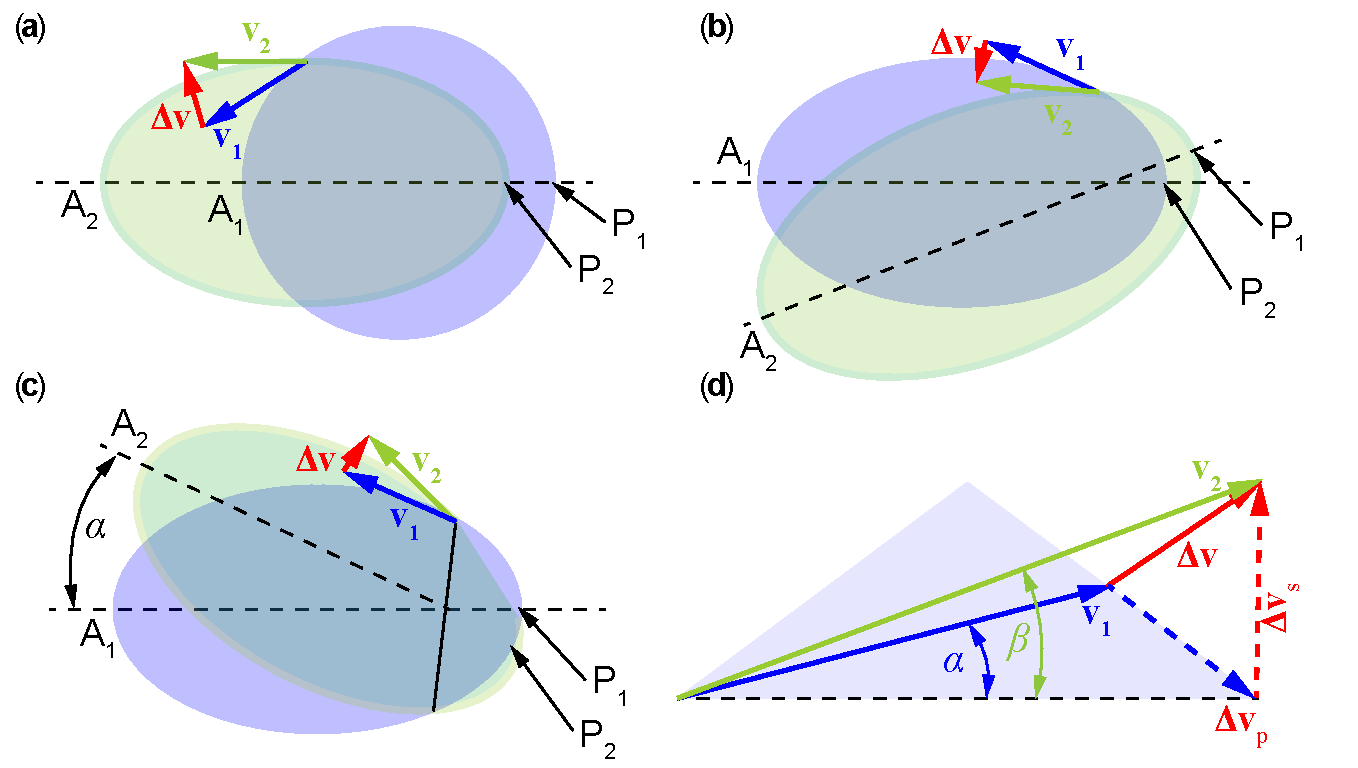
\includegraphics[width=\textwidth]{Bahnmanoever.pdf} 
	\caption[Wirkung der Geschwindigkeits�nderung auf Satellitenbahnen.]{Wirkung der Geschwindigkeits�nderung auf Satellitenbahnen. \fa �nderung der Exzentrizit�t. \fb �nderung der (Richtung) der Apsidenlinie. \fc �nderung der Inklination. \fd Vektorielle Addition der Geschwindigkeiten beim impulsiven Man�ver. Der Winkel $\alpha$ liegt wie $\Delta \vec{v}_\text{p}$ in der urspr�nglichen Bahnebene, der Winkel $\beta$ ebenso wie $\Delta \vec{v}_\text{s}$ senkrecht zur urspr�nglichen Bahnebene.}
	\label{abb:adyn_manenvers_overview}
\end{figure}

F�r impulsive Schubphasen kann die Wirkung der Geschwindigkeits�nderung je nach vektorieller Addition nach folgenden Gesichtspunkten unterteilt werden (\figref{adyn_manenvers_overview}).
\begin{enumerate}
    \item [1)] Koplanare Transfers, \dh die Bahnebene bleibt erhalten, wobei es entweder zu einer 
\begin{itemize}
        \item  �nderung der Exzentrizit�t bis hin zum �bergang in eine andere Bahnform oder
        \item  einer �nderung der Apsidenlinie kommt, oder alternativ zu einer
\end{itemize}
    \item [2)] �nderung der Inklination der Bahn f�hrt.
\end{enumerate}
Wir wollen uns zun�chst koplanare Transfers/Man�ver anschauen.

\subsubsection{Hohmann-Transfer}\label{kap:adyn_hohmann_transfer}

Als erstes Beispiel f�r ein impulsives koplanares Man�ver betrachten wir den Hohmann\indexp{Hohmann, Walter}\footnote{Walter Hohmann (1880--1945) war ein st�dtischer Baurat in Essen und besch�ftigte sich nebenberuflich mit Himmelsmechanik und Raumfahrt. Den nach ihm benannten Transfer zwischen zwei Satellitenbahnen beschrieb er bereits 1925 in seinem Buch "`Die Erreichbarkeit der Himmelsk�rper"'.}-Transfer. Der Hohmann-Transfers besteht darin, einen Satelliten aus einer niedrigeren (kreisf�rmigen) Umlaufbahn durch zwei Schubman�ver mit $\Delta v_1$  und $\Delta v_2$ auf eine Kreisbahn mit gr��erem Radius zu "`heben"' (\figref{adyn_hohmann_transfer}a).
Wir wollen als Beispiel berechnen, wie man einen Satelliten von einer Kreisbahn mit $h_1$ auf eine Kreisbahn der H�he $h_2$ bringen kann. \\
Dann muss der Satellit vor \bzw nach den Man�vern die Geschwindigkeiten 
\begin{align}
    v_1 = \sqrt{\frac{G\,m_\text{E}}{r_1}}= \sqrt{\frac{G\,m_\text{E}}{R_\text{E}+h_1}} ~~\text{\bzw}~~ 
		v_2 = \sqrt{\frac{G\,m_\text{E}}{r_2}}= \sqrt{\frac{G\,m_\text{E}}{R_\text{E}+h_2}} \label{eq:adyn_hohmann01}
\end{align}
haben.
\begin{figure}[H]
	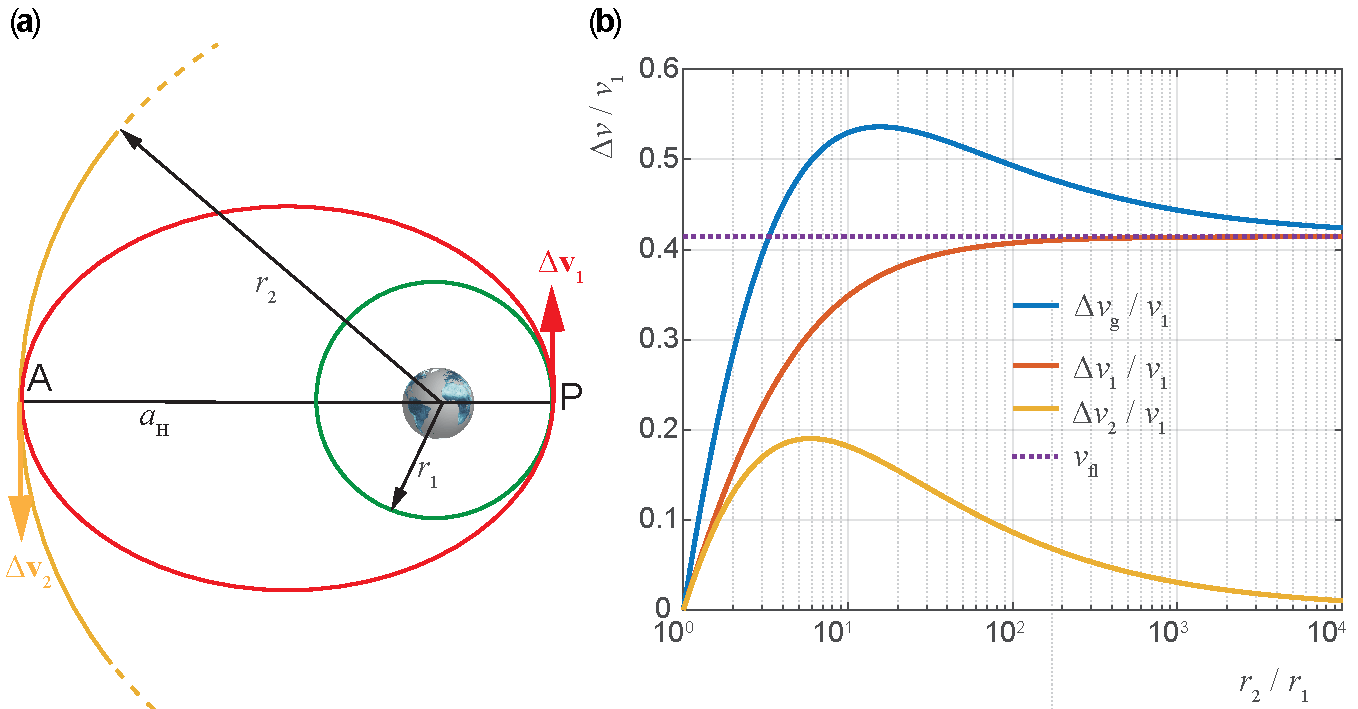
\includegraphics[width=\textwidth]{HohmannTransfer.pdf} 
	\caption[Hohmann-Transfer Prinzip und Geschwindigkeits�nderung.]{\fa Hohmann-Transfer Prinzip und \fb Geschwindigkeits�nderung bei Hohmann-Transfer als Funktion der Radius�nderung.}
	\label{abb:adyn_hohmann_transfer}
\end{figure}
Durch das erste Bahnman�ver mit $\Delta v_1$ kommt der Satellit aus einer Kreisbahn auf eine Transferellipse (Hohmann-Ellipse, \figref{adyn_hohmann_transfer}a), deren gro�e Halbachse durch 
\begin{align}
    a_\text{H} = \frac{1}{2}\,\lk r_1+r_2 \rk \label{eq:adyn_hohmann02}
\end{align}
gegeben ist. Nach der \gls{visvivaadyn} \eqref{eq:hm_vis-viva} \bzw \eqref{eq:adyn_orbit03} ergeben sich dann f�r diese Ellipse folgende Perig�ums- und Apog�umsgeschwindigkeiten:
\begin{subequations}
\begin{align}
    v_\text{P} &= \sqrt{G\,m_\text{E}}\,\sqrt{\frac{2}{r_1}-\frac{1}{\frac{1}{2}\,\lk r_1+r_2\rk}} = \sqrt{\frac{G\,m_\text{E}}{a_\text{H}}\,\frac{r_2}{r_1}} \,,\label{eq:adyn_hohmann03a}\\
    v_\text{A} &= \sqrt{G\,m_\text{E}}\,\sqrt{\frac{2}{r_2}-\frac{1}{\frac{1}{2}\,\lk r_1+r_2\rk}} = \sqrt{\frac{G\,m_\text{E}}{a_\text{H}}\,\frac{r_1}{r_2}}\,.\label{eq:adyn_hohmann03b}
\end{align}
\end{subequations}
Im Apog�um\index{Apog�um} der Transferellipse muss eine zweite Schubphase mit $\Delta v_2$ erfolgen, die aus der Ellipsenbahn wieder eine Kreisbahn mit der Geschwindigkeit $v_2$ nach \eqref{eq:adyn_hohmann01} macht, \dh wir haben insgesamt eine Geschwindigkeits�nderung von 
\begin{align}
    \Delta v = \Delta v_1+ \Delta v_2 = \lk v_\text{P}-v_1\rk +\lk v_2-v_\text{A}\rk\,.\label{eq:adyn_hohmann04}
\end{align}
In \figref{adyn_hohmann_transfer}b ist der Antriebsbedarf $\Delta v$ als Funktion des Radienverh�ltnisses $r_2/r_1$ dargestellt. Man erkennt, dass f�r bestimmte Radienverh�ltnisse der gesamte Geschwindigkeitsbedarf $\Delta v$ gr��er als die \gls{vescape} werden kann (\probref{adyn_manoevers1}).
%BEISPIEL 1 %%%%%%%%%%%%%%%%%%%%%%%%%%%%%%%%%%%%%%%%%%%%%%%%%%%%%%%%%%%%%%%%%%%%%%%%%%%%%%%%%
\begin{example}{Hohmann-Transfer f�r kleine Bahn�nderungen}  
Wir wollen jetzt noch eine N�herung f�r den Geschwindigkeitsbedarf beim Hohmann-Transfer f�r kleine Bahn�nderungen $\Delta r$ herleiten.
Wir erhalten f�r kleine Bahn�nderungen
	\[\frac{\Delta r}{r_1} = \frac{r_2-r_1}{r_1} \approx \frac{\Delta r}{r}~~\rightarrow~~r_2 \approx \Delta r+ r_1\,.
\]
Unter Verwendung von $a_\text{H} = r_1 +\Delta r / 2$ folgt damit:
\begin{align}
\begin{split}
    v_2 &= \sqrt{\frac{G\,m_\text{E}\,r_1}{r_2\,r_1}} = v_1\,\sqrt{\frac{r_1}{r_2}} \approx v_1 \,\sqrt{\frac{r_1}{r_1+\Delta r}} \approx v_1\,\lk 1-\frac{1}{2}\,\frac{\Delta r}{r}\rk\,,\\ 
    v_\text{P}&= v_1\,\lk 1+\frac{1}{4}\,\frac{\Delta r}{r}\rk\;, ~~~v_\text{A} = v_1\,\lk 1-\frac{3}{4}\,\frac{\Delta r}{r}\rk\,, 
\end{split} \label{eq:adyn_hohmann05}
\end{align}
woraus folgt:
\begin{align}
    \Delta v &= \killA{v_1} + \frac{v_1}{4}\,\frac{\Delta r}{r}-\killA{v_1} + \killA{v_1} - \frac{v_1}{2}\,\frac{\Delta r}{r}-\killA{v_1} + \frac{3}{4}\,v_1\,\frac{\Delta r}{r} \ = \frac{1}{2}\,v_1\,\frac{\Delta r}{r} \,. \label{eq:adyn_hohmann06}
\end{align} 
\end{example} \label{bsp:adyn_hohmann_klein}
%BEISPIEL %%%%%%%%%%%%%%%%%%%%%%%%%%%%%%%%%%%%%%%%%%%%%%%%%%%%%%%%%%%%%%%%%%%%%%%%%%%%%%%%%%

\subsubsection{Hohmann-, Oberth- und Edelbaum-Transfers nach Unendlich}\label{kap:adyn_oberth_edelbaum}

\begin{figure}[H]
	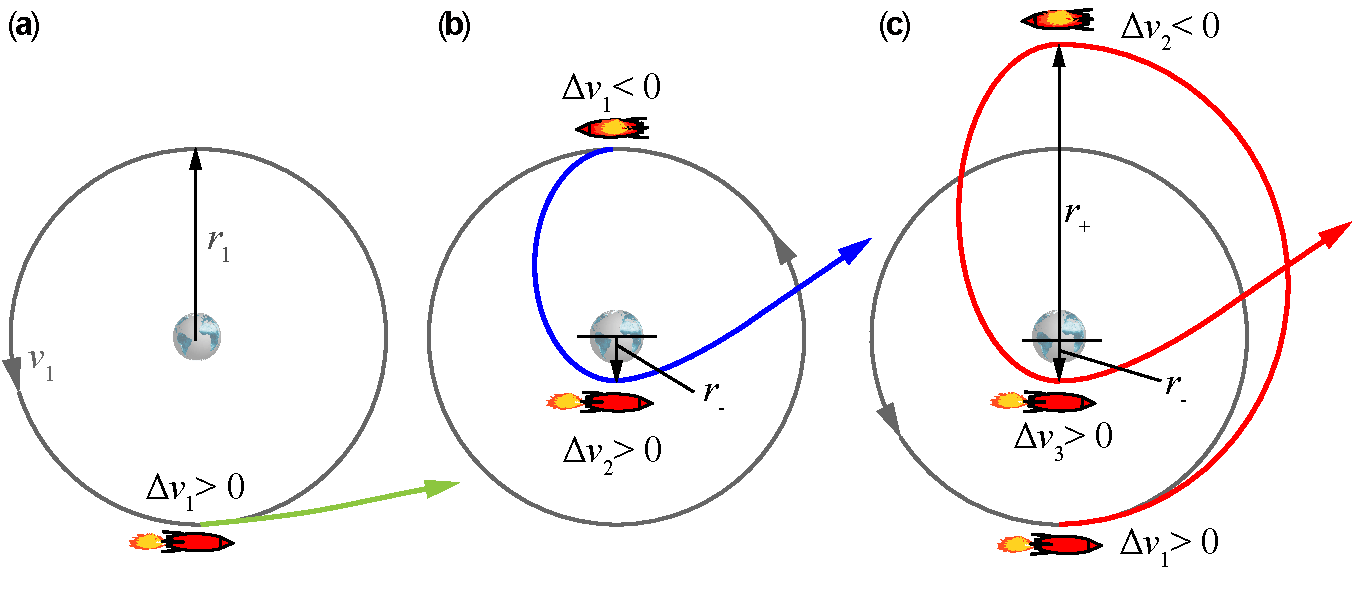
\includegraphics[width=\textwidth]{TransfersInfin01.pdf} 
	\caption[Hohmann-, Oberth- und Edelbaum-Transfers nach Unendlich.]{\fa Hohmann-, \fb Oberth- und \fc Edelbaum-Transfers nach Unendlich ($\infty$).}
	\label{abb:adyn_Oberth_transfer1}
\end{figure}

In vorherigen \kap{adyn_hohmann_transfer} hatten wir den Hohmann-Transfer von Satelliten von einer kreisf�rmigen Ausgangsbahn mit Radius $r_1$ auf eine elliptische Bahn mit der gro�en Halbachse $a_\text{H}$ und anschlie�end auf eine Kreisbahn mit $r_2$ untersucht, wobei $a_\text{H} = \frac{1}{2}\,\lk r_1+r_2\rk$ war. \\
Man kann sich jetzt die Frage stellen, wie gro� die notwendige Geschwindigkeits�nderung sein muss, damit der Satellit aus der Umlaufbahn $r_1$ nach $r_2=\infty$ kommt, also den Gravitationsbereich der Erde (\bzw des jeweiligen Zentralk�rpers) verl�sst. Wie gro� ist seine Flugzeit in einem solchen Fall, bis der Satellit \zb einen Abstand $200\,r_1,\,500\,r_1,\,1000\,r_1$ von der Erde erreicht (siehe auch \probref{adyn_manoevers2})?\\
Man kann sich auch �berlegen, dass es neben diesem sogenannten direkten Transfer auf die Endgeschwindigkeit $v_\infty$ (im Prinzip ein entarteter Hohmann-Transfer auf eine Hyperbel) zwei m�gliche weitere Transfers mit insgesamt zwei \bzw drei impulsiven Schubman�vern geben kann. Diese werden als Oberth-\indexp{Oberth, Hermann Julius} \bzw Edelbaum\indexp{Edelbaum, Theodore}\footnote{Theodore N. Edelbaum war ein US-amerikanischer Astrodynamiker und Raumfahrtspezialist.}-Transfers oder auch Zwei- \bzw Drei-Impuls-Transfers bezeichnet (\figref{adyn_Oberth_transfer1}).\\
Wir berechnen die notwendigen $\Delta v$ f�r die 3 F�lle, die entsprechende Flugzeit und den Treibstoffverbrauch und folgen dabei der Darstellung in \cite{Blanco2021}. Bei der L�sung benutzen wir:
\begin{enumerate}
    \item Die Energiegleichung (Notation entsprechend \kap{hm_bewegungsgl}):
    \begin{align}
        H = \frac{1}{2}\,v^2 -\frac{G\,m_\text{E}}{r}\,. \label{eq:adyn_escape01}
    \end{align}
		\item Die asymptotische Geschwindigkeit $v_\infty$ im Unendlichen ergibt sich dann:
    \begin{align}
        \frac{1}{2}\,v_\infty{}^2 &= \frac{1}{2}\,v_\text{Start} - \frac{G\,m_\text{E}}{r_\text{Start}}~~~\rightarrow ~~~ v_\text{Start} = \sqrt{\frac{2\,G\,m_\text{E}}{r_\text{Start}} + v_\infty{}^2} \,. \label{eq:adyn_escape02} 
    \end{align}
    Hierin sind $v_\text{Start},\,r_\text{Start}$ die Geschwindigkeit \bzw der Radius nach dem Starten des Man�vers. Man beachte, dass $v_\text{Start}$ f�r $v_\infty > 0$ verschieden von der f�r die Erde definierten Fluchtgeschwindigkeit $v_\text{F} = \sqrt{2\,G\,m_\text{E} / R_\text{E}}$ ist.
		\item Die Definition des Drehimpulses f�r eine Kreisbahn \bzw Ellipsenbahn (A\,Apog�um\,,\,P Perig�um)\index{Apog�um}\index{Perig�um} lautet:
    \begin{align}
    \begin{split}
        L &= r_1\,v_1~~~~ \text{Kreisbahn}\,,~~~\text{\bzw}~~~ L = r_\text{A}\,v_\text{A} = r_\text{P}\,v_\text{P}~~~~ \text{Ellipse} \,,\\
				&\text{mit} ~~ r_\text{P},\,r_\text{A} ~~~\text{Abstand zum Perig�um \bzw Apog�um}\,.
    \end{split}\label{eq:adyn_escape03} 
    \end{align}
    \item F�r die Geschwindigkeit beim Apo- \bzw Perig�um kann man aus der Drehimpulserhaltung leicht ableiten:
    \begin{align}
        v_\text{A} &= \sqrt{\frac{G\,m_\text{E}}{r_\text{A}}} \,\sqrt{\frac{2}{1+r_\text{A}/r_\text{P}} }\, ~~~ \text{\bzw}~~~
        v_\text{P} = \sqrt{\frac{G\,m_\text{E}}{r_\text{P}}} \,\sqrt{\frac{2}{1+r_\text{P}/r_\text{A}} }\,. \label{eq:adyn_escape04}
    \end{align}
\end{enumerate}		
		Wir schauen uns nun die einzelnen Transfers an, wobei wir den Radius der Ausgangsbahn jetzt mit $r_0$ bezeichnen wollen.
\begin{itemize} 
		\item \underline{Fall A:} Direkter Transfer aus einer Kreisbahn mit Radius $r_1$ (Hohmann-Transfer nach $\infty$) \\
    Aus \eqref{eq:adyn_escape02} erhalten wir
    \begin{align}
		\begin{split}
        v_\text{Start} &= v_1 +\Delta v_\text{A} = \sqrt{\frac{2\,G\,m_\text{E}}{r_1} + v_\infty{}^2}\qquad\text{und mit} \qquad v_1 = \sqrt{\frac{G\,m_\text{E}}{r_1}}   \,,\\
         \rightarrow ~~~~ \Delta v_\text{A} &= v_1\,\lk \sqrt{2+\frac{v_\infty{}^2}{v_1{}^2}}-1\rk = v_1\,\lk \sqrt{2+\frac{v_\infty{}^2\,r_1}{G\,m_\text{E}}}-1\rk \,.
		\end{split} \label{eq:adyn_escape06}
    \end{align}
    \item \underline{Fall B:} Zwei-Impuls-Transfer (Oberth-Transfer)\\
		Die physikalischen Grundlagen des Oberth-Effektes\index{Oberth-Effekt} und damit des Oberth-Transfers sind ausf�hrlich in \probref{adyn_rocket_analogy} behandelt und sollen hier als bekannt voraus gesetzt werden.
    \begin{itemize}
        \item F�r den ersten Impuls, bei dem es zu einer Abbremsung aus der initialen Kreisbahn mit $r_1$ auf eine kleinere Ellipsenbahn mit Perig�umsabstand $r_\text{-}$ kommt, finden wir am Punkt $A$ (Apog�um)
        \begin{align}
            \Delta v_{\text{B},1} &= v_\text{A} -v_1 = \sqrt{\frac{G\,M}{r_1}}\,\lk \sqrt{\frac{2}{1+\frac{r_1}{r_\text{-}}}}\rk-v_1 = -v_1\,\lk 1-\sqrt{\frac{2}{1+\frac{r_1}{r_\text{-}}}}\rk \label{eq:adyn_escape07}\,.
        \end{align}
        \item Beim Perig�um $P$, wo $r=r_\text{-}$ ist und der zweite Impuls erfolgt, finden wir
        \begin{align}
            \Delta v_{\text{B},2} &= v_\text{Start} - v_\text{P} = \sqrt{\frac{2\,G\,m_\text{E}}{r_\text{-}} + v_\infty{}^2} - \sqrt{\frac{G\,m_\text{E}}{r_\text{-}}}\,\sqrt{\frac{2}{1+r_\text{-} / r_1}}\nonumber \\
            &= \sqrt{\frac{G\,m_\text{E}}{r_1}}\,\lk \sqrt{2+\frac{v_\infty{}^2\,r_\text{-}}{G\,m_\text{E}}} - \sqrt{\frac{2}{1+r_\text{-} / r_1}}\rk \,. \label{eq:adyn_escape08}
        \end{align}
        \item Der gesamte notwendige Antriebsbedarf ist dann
        \begin{align}
            \Delta v_\text{B} = |\Delta v_\text{B,1}| + \Delta v_\text{B,2} = v_1\,\lk 1+\sqrt{\frac{v_\infty{}^2}{v_1{}^2} + \frac{2r_1}{r_\text{-}}} - \sqrt{2+\frac{2r_1}{r_\text{-}}}\rk \label{eq:adyn_escape09}\,.
        \end{align}
    \end{itemize}
    \item \underline{Fall C:} Drei-Impuls-Transfer (Edelbaum-Transfer)
    \begin{itemize}
        \item Im ersten Schritt geht das Raumschiff auf eine gr��ere elliptische Bahn mit einer gro�en Halbachse $r_\text{+}$:
        \begin{align}
            \Delta v_\text{C,1} = v_1\,\lk \sqrt{\frac{2}{1+\frac{r_1}{r_\text{+}}}} -1\rk\,. \label{eq:adyn_escape10} 
        \end{align}
        \item Im zweiten Schritt wird es wieder auf eine deutlich kleinere Bahn mit Radius $r_\text{Ed2}$ gebracht (durch Abbremsen):
        \begin{align}
            \Delta v_\text{C,2} = -\sqrt{\frac{G\,m_\text{E}}{r_\text{+}}}\,\lk \sqrt{\frac{2}{1+r_\text{+} / r_1}} - \sqrt{\frac{2}{1+r_\text{+} / r_\text{-}}}\rk \,. \label{eq:adyn_escape11} 
        \end{align}
        \item Im dritten Schritt wird das Raumschiff wieder beschleunigt:
        \begin{align}
            \Delta v_\text{C,3} = \sqrt{\frac{G\,m_\text{E}}{r_\text{-}}}\,\lk \sqrt{2+\frac{v_\infty{}^2\,r_\text{-}}{G\,m_\text{E}}} - \sqrt{\frac{2}{1+r_\text{-}/ r_\text{+}}}\rk\,.\label{eq:adyn_escape12} 
        \end{align}
        \item Die gesamte Geschwindigkeits�nderung ist:
        \begin{align}
            \Delta v_\text{C} &= \Delta v_\text{C,1} + |\Delta v_\text{C,2}| + \Delta v_\text{C,3} \nonumber \\
            &= v_1\,\lk \sqrt{\frac{v_\infty{}^2}{v_1{}^2} + \frac{2r_1}{r_\text{-}}} + \sqrt{2 + \frac{2r_1}{r_\text{+}}} - \sqrt{\frac{2r_1}{r_\text{-}}+\frac{2r_1}{r_\text{+}}}- 1\rk\,.\label{eq:adyn_escape13} 
        \end{align}
    \end{itemize}
\end{itemize}
Man kann nun vergleichen, wie sich die $\Delta v$ f�r die verschiedenen F�lle verhalten  (\figref{adyn_Oberth_transfer2}) und erkennt, dass f�r gr��ere $v_\infty$ das Edelbaum-Man�ver einen geringeren Antriebsbedarf (und damit geringeren Treibstoffbedarf) hat als der Oberth- und auch der direkte Transfer. 
Aus \eqref{eq:adyn_escape13} erh�lt man durch Invertierung auch eine Beziehung f�r $v_\infty\,\lk v_1,r_1,r_\text{-},r_\text{+}\rk$ bei gegebenen Treibstoffvorrat $\Delta v$:
\begin{align}
    v_\infty = v_1\,\sqrt{ \lek 1+\frac{\Delta v}{v_1} + \sqrt{\frac{2r_1}{r_\text{-}} + \frac{2r_1}{r_\text{+}}} - \sqrt{2+\frac{2r_1}{r_\text{+}}} \rek^2 - \frac{2\,r_1}{r_\text{-}} }\,.\label{eq:adyn_escape14} 
\end{align}
F�r $r_\text{+} = r_1$ ergibt sich die Beziehung f�r den Oberth-Transfer, f�r $r_\text{-} = r_\text{+} = r_1$ die f�r den direkten Transfer.
%BEISPIEL 2 %%%%%%%%%%%%%%%%%%%%%%%%%%%%%%%%%%%%%%%%%%%%%%%%%%%%%%%%%%%%%%%%%%%%%%%%%%%%%%%%%
\begin{example}{Flugbahnen und Flugzeiten f�r die Hohmann-Oberth-Edelbaum-Transfers}  
Zum Schluss adressieren wir die Frage, welches das Flugman�ver (Hohmann-, Oberth- oder Edelbaum-Transfer) mit dem geringsten Treibstoffverbrauch \bzw mit der k�rzesten Flugzeit ist.
Die Energie des Systems Raumschiff und ausgestr�mtes Gas nach dem jeweiligen i-ten Schubimpuls ist:
\begin{align}
	E_\text{g} &= T_\text{g, i} + \Delta E_\text{chem} = -\frac{1}{2}\, m_\text{i} v_1{}^2 + \frac{1}{2}\, \lk m_\text{i} - m_\text{f} \rk v_\text{G}{}^2 \nonumber \\
	           &= -\frac{1}{2}\, m_\text{i} v_1{}^2 + \frac{1}{2}\,  m_\text{i}\,v_\text{G}{}^2 \lk 1 - \e^{\lk - \Delta v / v_\text{G} \rk} \rk \,. \label{eq:adyn_oberth31}
\end{align}
Hierin ist wie bisher $m_\text{i}$ die Gesamtmasse des Raumschiffs inklusive Treibstoff vor dem Schubman�ver, $m_\text{f}$ die Masse danach, $v_\text{G}$ die Ausstr�mgeschwindigkeit des Treibstoffgases und $\Delta E_\text{chem} $ die w�hrend des Schubs umgesetzte chemische Energie des Treibstoffs. Wenn man $v_\text{G} = \kappa\,v_1$ setzt, dann kann man die �nderung der kinetischen Energie des Raumschiffs pro impulsivem Schubman�ver relativ einfach berechnen.\\ %Dies werden wir in \probref{adyn_manoevers1} tun. \\
F�r die Berechnung der Flugzeiten muss man beachten, dass sich die Gesamtzeit aus Segmenten einer hyperbolischen Bahn und Segmenten von elliptischen Bahnen (genauer halben Ellipsen) zusammensetzt. Die Berechnung der Halbellipsen-Zeiten (\zb von $r_\text{out}$ bis $r_\text{in}$) ist nach dem 3. Keplerschen Gesetz:
\begin{align}
	t_\text{ell} = \frac{1}{2}\,2\pi \sqrt{\frac{a^3}{G\,m_\text{E}}} = \frac{\pi}{2} \sqrt{\frac{\lk r_\text{A} + r_\text{P} \rk^3}{2\,G\,m_\text{E}}} \,. \label{eq:adyn_oberth32}
\end{align}
Die Berechnung des hyperbolischen Abschnitts ist etwas komplexer. Wir starten dazu von der Gleichung f�r den Radialanteil der Geschwindigkeit (vgl. \eqref{eq:hm_allg_ZK_2}):
\begin{align}
	v_r{}^2 = \lk \frac{\D r}{\D t}\rk^2 = v_\infty{}^2 + 2 \,\frac{G\,m_\text{E}}{r} - \frac{L^2}{r^2}  \,. \label{eq:adyn_oberth33}
\end{align}
Wir wissen, dass am Perig�um gilt:
\begin{align}
   \frac{\D r}{\D t} &= 0 ~~~\rightarrow~~~ L^2 = v_\infty{}^2\,r_\text{P}{}^2 + 2 \,G\,m_\text{E}\,r_\text{P} ~~~\text{und erhalten somit} \nonumber \\
	 \frac{\D r}{\D t} &= \sqrt{ v_\infty{}^2 + 2 \,\frac{G\,m_\text{E}}{r} - \frac{v_\infty{}^2\,r_\text{P}{}^2 + 2 \,G\,m_\text{E}\,r_\text{P}}{r^2}} \,.  \label{eq:adyn_oberth34}
\end{align}
Diese DGL 1. Ordnung kann man numerisch mit den �blichen Verfahren in \matlab{}\, integrieren, alternativ kann man die inverse Funktion $t(r)$ durch Integration von
\begin{align}
	 \frac{\D t}{\D r} = \frac{r}{\sqrt{ v_\infty{}^2 \lk {r^2 -r_\text{P}{}^2}\rk + 2 \,G\,m_\text{E} \lk {r -r_\text{P}}\rk }} \label{eq:adyn_oberth35}
\end{align}
berechnen. Mit Hilfe einer Integraltafel \cite{Gradshteyn1980} findet man:
\begin{align}
\begin{split}
	 t_\text{hyp}(r, r_\text{P}) &= \frac{G\,m_\text{E}}{v_\infty{}^3} \lek \sqrt{\lk 1+ \frac{r\,v_\infty{}^2}{G\,m_\text{E}}\rk^2 - \lk 1 + \frac{r_\text{P}\,v_\infty{}^2}{G\,m_\text{E}}\rk^2 }\rek + \ldots \\
	      &~~~ + \frac{G\,m_\text{E}}{v_\infty{}^3} \ln{\lek \frac{G\,m_\text{E} + v_\infty{}^2\,r}{v_\infty\, \sqrt{ v_\infty{}^2 \lk {r^2 -r_\text{P}{}^2}\rk + 2 \,G\,m_\text{E} \lk {r -r_\text{P}}\rk }}\rek}\\
				&= \frac{T_0}{2\pi} \frac{v_1{}^3}{v_\infty{}^3} \lek \sqrt{\lk 1 + \frac{r\,v_\infty{}^2}{r_1\,v_1{}^2} \rk^2 - \lk 1 + \frac{r_\text{P}\,v_\infty{}^2}{r_1\,v_1{}^2} \rk^2 } -
				    \cosh^{-1} {\lk \frac{1 + \frac{r\,v_\infty{}^2}{r_1\,v_1{}^2}}{1 + \frac{r_\text{P}\,v_\infty{}^2}{r_1\,v_1{}^2} } \rk} \rek \,.
\end{split} \label{eq:adyn_oberth36}
\end{align}
\label{bsp:adyn_transfers_times}
F�r die weitere Diskussion verweisen wir auf \probref{adyn_manoevers3}.\\

\end{example}
%BEISPIEL %%%%%%%%%%%%%%%%%%%%%%%%%%%%%%%%%%%%%%%%%%%%%%%%%%%%%%%%%%%%%%%%%%%%%%%%%%%%%%%%%%

\begin{figure}[H]
	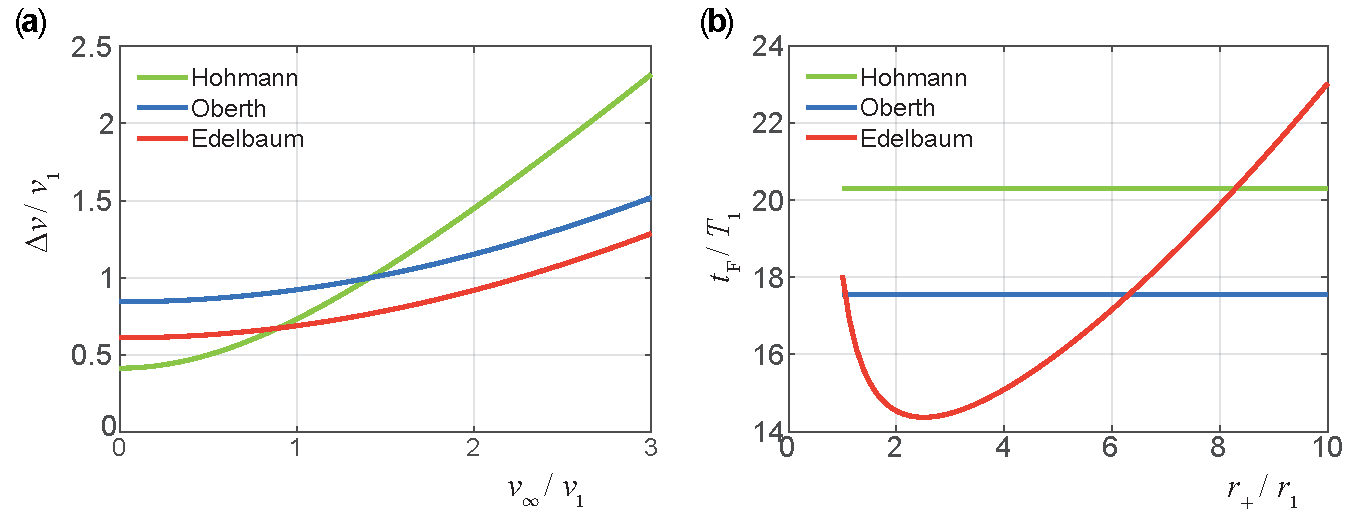
\includegraphics[width=\textwidth]{TransfersInfin02.pdf} 
	\caption[Geschwindigkeitsbedarf und Flugzeiten beim Transfer nach $\infty$.]{\fa Geschwindigkeitsbedarf f�r verschiedene zu erzielende Endgeschwindigkeiten beim Hohmann-, Oberth- \bzw Edelbaum-Transfer nach $\infty$. Man sieht, dass ab einer bestimmten zu erreichenden Endgeschwindigkeit das Geschwindigkeitsbudget f�r den Oberth- und Edelbaum-Transfer kleiner ist als das f�r den direkten Hohmann-Transfer. \fb Flugzeiten bis zu $r=200\,r_1$ beim Hohmann-, Oberth- \bzw Edelbaum-Transfer. Als variabler Parameter wurde der �u�ere Radius $r_{+}$ genommen, der innere Radius wurde als fix mit $r_{-}=0.05\,r_1$ gesetzt und der Schubparameter wurde mit $\Delta v/v1 = 1.1$ angenommen. Man erkennt, dass es f�r $r_{+}\approx 2.5\,r_1$ ein absolutes Minimum der Flugzeit f�r den Edelbaum-Transfer gibt. Danach f�hrt die l�ngere Flugzeit auf der Halbellipse von $r_{+}$ nach $r_{-}$ zu insgesamt l�ngeren Flugzeiten. (Nach \cite{Blanco2021}, siehe auch \probref{adyn_manoevers2}.)} \label{abb:adyn_Oberth_transfer2}
\end{figure}
Das Ergebnis der zeitlichen Entwicklung der verschiedenen Transfers ist in \probref{adyn_manoevers2} explizit durchgerechnet und das Ergebnis im Vergleich der verschiedenen Transfers in \figref{adyn_Oberth_transfer2} zu sehen. 

\subsection{Interplanetare Raumfl�ge zu den Nachbarplaneten der Erde}\label{kap:adyn_flight_venus_mars}

Wir wollen in diesem Kapitel Raumfl�ge zu Mars und Venus untersuchen und zun�chst stark vereinfachende Annahmen treffen, um Grundprinzipien bei der Planung einer solchen Mission zu verdeutlichen. Insbesondere sollen
\begin{enumerate}
    \item [1.] alle Bewegungen (Planeten, Raumsonde) koplanar in der Ekliptik stattfinden,
		\item [2.] die Planetenbahnen als kreisf�rmig angenommen werden und
		\item [3.] der Flug zum Nachbarplaneten �ber eine Hohmann-Ellipse erfolgen.
\end{enumerate}
Zun�chst betrachten wir den Flug zur Venus, f�r welchen gilt:
\begin{align}
\begin{split}
    \upsilon_\text{E}  &= \upsilon_\text{E}\lk t_0\rk + n_\text{E}\,\lk t-t_0\rk = \upsilon_\text{E,0} + n_\text{E}\,t\,,\\
    \upsilon_\text{V}  &= \upsilon_\text{V}\lk t_0\rk + n_\text{V}\,\lk t-t_0\rk = \upsilon_\text{V,0} + n_\text{V}\,t\,.
\end{split} \label{eq:adyn_PlFlights01}
\end{align} 
Hierin sind $n_\text{E},\,n_\text{V},\,n_\text{M}$ die mittleren Bewegungen\index{Bewegung!mittlere} der Planeten Erde, Venus \bzw f�r sp�ter auch Mars (siehe Tabelle \ref{tab:hm_bahnparameter}), die sich nach \eqref{eq:adyn_Bahnpara05} berechnet. Die Differenz der wahren Anomalien $\psi = \upsilon_\text{V} -\upsilon_\text{E}$ wird als Phasenwinkel zwischen Venus und Erde bezeichnet. Dessen zeitliche Entwicklung lautet:
\begin{align}
    \psi = \psi_0 + \lk n_\text{V} - n_\text{E}\rk\,t ~~~~ \text{mit} ~~~~ \psi_0 = \upsilon_\text{V,0} - \upsilon_\text{E,0}\,. \label{eq:adyn_PlFlights02}
\end{align}
Aus \eqref{eq:adyn_PlFlights02} folgt die bereits in der \probref{hm_sideric_period_mars} hergeleitete synodische Periode\index{Periode!Synodische} eines Planeten (hier der Venus). Diese synodische Periode ergibt sich als die Zeit, die verstreicht, bis der Phasenwinkel zwischen den beiden betrachteten Himmelsk�rpern wieder den gleichen Wert hat.
\begin{align}
    \psi_0 +2k\pi &= \psi_0 +\lk n_\text{V} - n_\text{E}\rk\,T_\text{syn}\nonumber\\
    \rightarrow ~~~~ T_\text{syn,V} &= \frac{2\pi}{n_\text{V}-n_\text{E}} = \frac{2\pi}{2\pi\,\lk \frac{1}{T_\text{P,V}} - \frac{1}{T_\text{P,E}}\rk} = \frac{T_\text{P,E} T_\text{P,V}}{T_\text{P,E} - T_\text{P,V}}\label{eq:adyn_PlFlights03}\,.
\end{align}
Analog gilt f�r den Mars:
\begin{align}
    T_\text{syn,M} = \frac{2\pi}{n_\text{E}-n_\text{M}} = \frac{T_\text{P,M} T_\text{P,E}}{T_\text{P,M} - T_\text{P,E}}\label{eq:adyn_PlFlights04}\,.
\end{align}
Da der Transfer �ber eine Hohmann-Ellipse mit der gro�en Halbachse $a_\text{H}$ erfolgen soll (vgl. auch \kap{adyn_hohmann_transfer}), findet man mit \figref{adyn_flight_venus_mars}b,c und dem sog. \gls{gravparadyn}\index{Gravitationsparameter}~$\mu_\text{S}=G\,m_\text{S}$ leicht den finalen Phasenwinkel $\psi_\text{f}$:
\begin{align}
\begin{split}
  a_\text{H} &= \frac{1}{2}\,\lk r_\text{E} + r_\text{M}\rk\,,\,~~t_\text{H} = \frac{1}{2} \frac{2\pi}{n_\text{H}} = \pi\,\sqrt{\frac{a_\text{H}{}^3}{\mu_\text{S}}}\,~~\text{und}~~ \pi = \psi_0 + n_\text{M}\,t_\text{H}\;, ~~~\\
 \psi_\text{f} &= \psi_0 + t_\text{H}\,\lk n_\text{M}-n_\text{E}\rk = \pi -n_\text{E}\,t_\text{H}\;.
\end{split}\label{eq:adyn_PlFlights05}
\end{align}
Damit liegen die Phasenwinkel zwischen Erde und Mars bei Start und Ankunft fest. Als Werte ergeben sich $t_\text{H} \approx 259\,\text{d}$, $\psi_0 \approx 44.3\degree$ und $\psi_\text{f} \approx -75.1\degree$. \\
Ein negativer Phasenwinkel $\psi_\text{f}$ bedeutet, dass der Mars \anf{hinter} der Erde liegt (\figref{adyn_flight_venus_mars}c), also $\upsilon_\text{f, M} < \upsilon_\text{f, E}$.

\begin{figure}[H]
	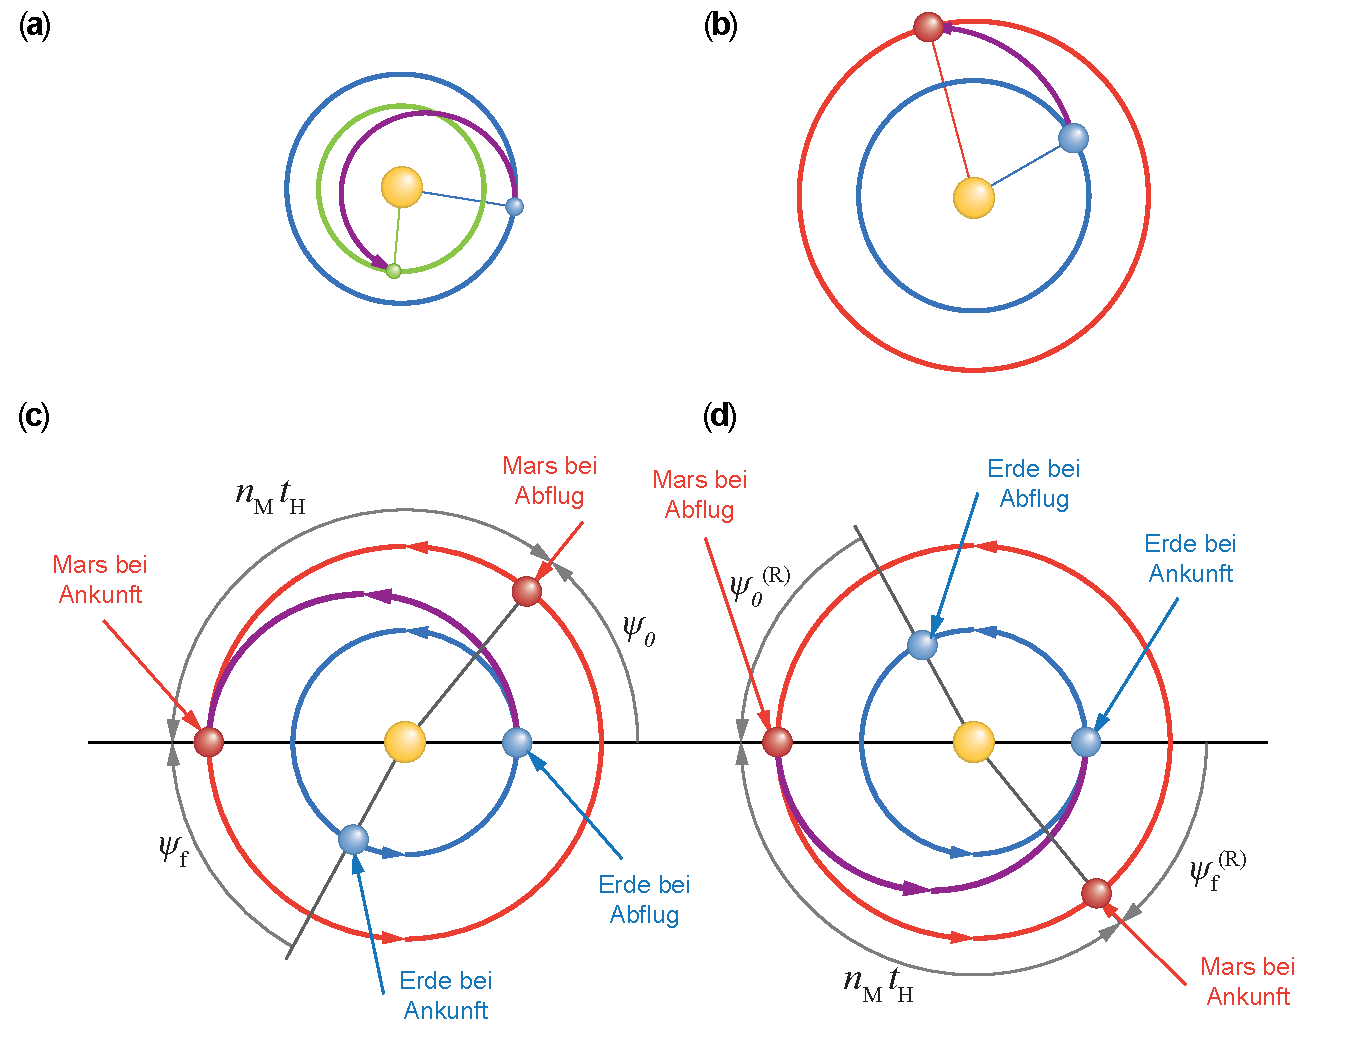
\includegraphics[width=\textwidth]{InterplanetarerTransfer.pdf} 
	\caption[Raumfl�ge zu Venus und Mars.]{Raumfl�ge zu Venus und Mars. \fa Raumflug zur Venus (ma�st�blich, Reisezeit 158 Tage). \fb Raumflug zum Mars (ma�st�blich, Reisezeit 115 Tage).  \fc Raumflug von der Erde zum Mars (nicht ma�st�blich). Beziehung der Phasenwinkel $\psi_0, \psi_\text{f}$ beim Hinflug von der Erde zum Mars. \fd Raumflug vom Mars zur Erde (nicht ma�st�blich). Beziehung der Phasenwinkel $\psi_0{}^\text{(R)}, \psi_0, \psi_\text{f}$ beim R�ckflug vom Mars zur Erde.}
	\label{abb:adyn_flight_venus_mars}
\end{figure}

F�r die R�ckkehr zur Erde geht man eine \anf{umgekehrte} Hohmann-Ellipse aus, was nichts anderes bedeutet als:
\begin{align}
    \psi_0{}^\text{(R)} = -\psi_\text{f}\,.\label{eq:adyn_PlFlights06R}
\end{align}
Die Raumsonde muss aber eine gewisse Zeit $t_\text{W}$ auf dem Mars warten, bis die Konstellation nach \eqref{eq:adyn_PlFlights06R} eintritt (\figref{adyn_flight_venus_mars}b). Wegen
\begin{align}
    0 = 2\psi_\text{f} + \lk n_\text{M} - n_\text{E} \rk \,t_\text{W} \label{eq:adyn_PlFlights06R1}
\end{align}
und der Forderung, dass $t_\text{W}>0$ ist, muss man gegebenenfalls einen Betrag von $2k\pi$ mit $k=0, \pm 1, \pm 2\ldots $ zu \eqref{eq:adyn_PlFlights06R1} addieren, woraus folgt:
\begin{align}
    t_\text{M, W} = \frac{2\psi_\text{f} + 2\,\pi\,N}{n_\text{E}-n_\text{M}} \,.\label{eq:adyn_PlFlights06M}
\end{align}
Wir erhalten $t_\text{W} \approx 454\,\text{d}$, was bedeutet, dass eine Reise zum Mars �ber Hohmann-Bahnen im Minimum:\
$t_\text{M, ges} = t_\text{H} + t_\text{W} +  t_\text{H} \approx 259\,\text{d} + 454\,\text{d} + 259\,\text{d} = 972\,\text{d}$\
dauern wird. Entsprechend erh�lt man f�r die Venus:
\begin{align}
    t_\text{V, W} = \frac{2\psi_\text{f} - 2\,\pi\,N}{n_\text{V}-n_\text{E}} \,,\label{eq:adyn_PlFlights06V}
\end{align}
mit $N=0$ die Werte $t_\text{V, ges} = t_\text{H} + t_\text{V, W} +  t_\text{H} \approx 146\,\text{d} + 117\,\text{d} + 146\,\text{d} = 409\,\text{d}$\,.\\

Wir wollen nun auch Fl�ge untersuchen und berechnen, die nicht �ber Hohmann-Ellipsen ablaufen und bei denen die Positionsvektoren der Zielplaneten auch nicht mehr in der Ekliptikebene liegen m�ssen. Ferner soll eine bestimmte Flugzeit vorgegeben sein. Es sind dann der vom Hohmann-Transfer verschiedene Antriebsbedarf $\Delta \vec{v}$ und die Parameter der Transferbahn zu bestimmen. Dies f�hrt auf das im n�chsten Kapitel behandelte Lambert-Problem.

\subsection{Lambert-Problem (Lambert-Transfer)}\label{kap:adyn_lambert_transfer}\index{Lambert-Transfer}\index{Lambert-Problem|textbf}

Das Lambert\indexp{Lambert, Johann Heinrich}\footnote{Johann Heinrich Lambert (1728 -- 1777) war ein hugenottischer Schweizer Mathematiker und Physiker, der sich auch mit Kartographie und Astronomie besch�ftigte. Neben dem Lambert-Problem der Himmelsmechanik ist auch das Lambert-Beersche Gesetz der Lichtabsorption nach ihm benannt.}\index{Lambert-Problem}-Problem lautet wie folgt:\\

Zur Zeit $t_1$ und $t_2$ seien zwei Positionsvektoren $\vec{r}(t_1) =\vec{r}_1$ und $\vec{r}(t_2) =\vec{r}_2$ eines K�rpers gegeben, der sich im Gravitationsfeld eines Zentralk�rpers befindet. Die Positionsvektoren werden dabei vom Zentralk�rper (Ursprung des Koordinatensystems) aus gemessen.\\
Man finde die L�sung $\vec{r}\lk t\rk$ und damit insbesondere auch die Geschwindigkeiten $\vec{v}(\vec{r}_1)$ und $\vec{v}(\vec{r}_2)$, welche der Differentialgleichung
\begin{align*}
    \ddot{\vec{r}} = -G\,m_\text{ZK}\,\frac{\vec{r}}{|\vec{r}|^2} = \mu\,\frac{\vec{r}}{|\vec{r}|^2} 
\end{align*}
gen�gen. Hierbei ist $m_\text{ZK}$ die Masse des Zentralk�rpers, um den die Bewegung erfolgt.\\
Das Lambert-Problem ist streng genommen kein reines Problem der Astrodynamik, sondern wurde bereits im 18. Jahrhundert von Lambert f�r die Himmelsmechanik aufgestellt und von Lagrange\indexp{Lagrange, Joseph-Louis} gel�st. �bertragen auf die Astrodynamik kann man auch formulieren: Gesucht ist die Raumkurve $\vec{r}\lk t\rk$ zwischen zwei Positionen im Raum $\vec{r}_1$ und $\vec{r}_2$, die in einer Zeit $t_\text{F}^* = t_2-t_1$, der sogenannten \gls{ToF} (ToF), durchflogen wird, wobei nur das Schwerefeld eines Zentralk�rpers wirkt. Die gesuchte Kurve muss daher ein Kegelschnitt sein, wobei wir uns hier auf elliptische Bahnen beschr�nken wollen. Da man folglich das Lambert-Problem auch als Bestimmung eines Transfer-Orbits zwischen zwei vorgegebenen Punkten verstehen kann, behandeln wir dieses Thema auch hier im Kapitel �ber Weltraumman�ver. Das Lambert-Problem ist eines der wichtigsten Probleme der Astrodynamik. Fragestellungen, wie die Planung von Bahnen f�r Rendezvous von Raumschiffen im Weltall, dass Abfangen von ballistischen Flugk�rpern oder Asteroiden oder auch die Konzeption interplanetarer Fl�ge gehen auf die L�sung des Lambert-Problems zur�ck. \\

\begin{figure}[H]
	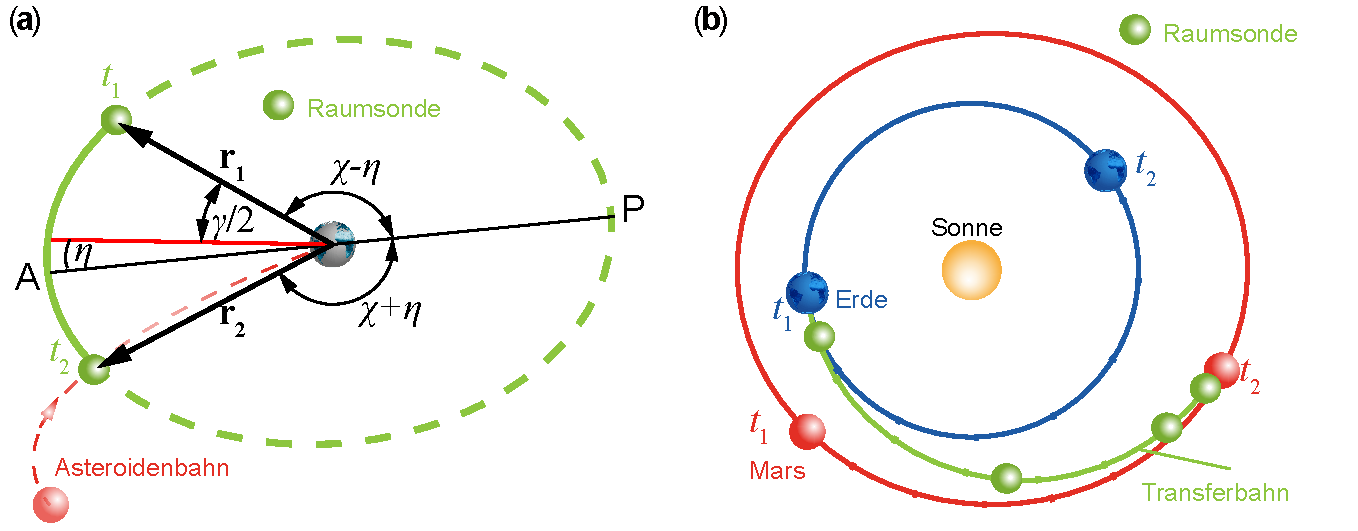
\includegraphics[width=\textwidth]{LambertProblem01Geometrie.pdf} 
	\caption[Lambert-Problem.]{\fa Geometrie des Lambert-Problems. Beispiel f�r ein Abfangen eines Asteroiden durch eine Raumsonde. \fb Anwendung des Lambert-Problems beim interplanetaren Flug zum Mars. Die Transferellipse zum Mars (Startzeitpunkt $t_1$ muss die Marsbahn zum Zeitpunkt $t_2$ auch genau dann schneiden/ber�hren, wenn der Mars sich an der entsprechenden Stelle befindet.}
	\label{abb:adyn_lambert_basic}
\end{figure}

In \figref{adyn_lambert_basic}a haben wir als Beispiel das Problem des "`Abfangens"' eines Asteroiden und in \figref{adyn_lambert_basic}b eine Planung eines Raumflugs zum Mars schematisch dargestellt, die wir in \probref{adyn_manoevers5} und  \probref{adyn_manoevers6} genauer behandeln wollen. Es gibt verschiedene Ans�tze zur L�sung des Lambert-Problems und noch heute erscheinen regelm��ig Originalarbeiten zu dem Thema. Im Wesentlichen geht es dabei um die (numerische) Optimierung der L�sungsverfahren und spezielle Probleme. Eine gute �bersicht �ber den aktuellen Stand findet sich f�r den interessierten Leser in \cite{Izzo2015} und \cite{sangra2021}, wobei die letztere Referenz auch explizit auf die \matlab-Modellierung eingeht.\\
Warum ist das Lambert-Problem so besonders? Gegeben sind beim Lambert-Problem wie oben ausgef�hrt, zwei Ortsvektoren $\vec{r}(t_1)$ und $\vec{r}(t_2)$ und die ToF. Gesucht sind die Bahnparameter und die Geschwindigkeiten $\dot{\vec{r}}(t_1)$ und $\dot{\vec{r}}(t_2)$ f�r die Kurve zwischen $\vec{r}(t_1)$ und $\vec{r}(t_2)$. Das ist ein sogenanntes \emph{Randwertproblem}\index{Randwertproblem|textbf}, welches wesentlich schwieriger zu l�sen ist als die bisher behandelten Anfangswertprobleme, bei denen alle Informationen zur Integration der Bewegungsgleichungen zum Anfangszeitpunkt bekannt waren. Im Gegensatz zu Anfangswertproblemen\index{Anfangswertproblem} haben Randwertprobleme nicht immer eine eindeutige L�sung. Die ausf�hrliche Behandlung von Randwertproblemen geht �ber den Umfang dieses Buches hinaus, wir empfehlen zur Vertiefung die Referenzen \cite{Arens2008, Fischer2014}.\footnote{Dem Lambert-Randwertproblem sind wir schon bei der Bestimmung der Bahnparameter aus zwei Ortsvektoren in \kap{adyn_orbits_determination_xwinkel} begegnet. Wir hatten dort lediglich die numerische Methodik angegeben, ohne auf das Randwertproblem einzugehen.} F�r das Lambert-Problem gibt es eine Reihe von L�sungsmethoden \cite{Izzo2015, sangra2021}, wir zeigen hier eine physikalisch sehr anschauliche, die auf \cite{Gatland2022} zur�ckgeht. In \probref{adyn_manoevers4} werden wir eine andere L�sungsmethode verwenden und auch auf weitere L�sungsmethoden verweisen. Wir f�hren mit Hilfe von \figref{adyn_lambert_basic} die folgenden Bezeichnungen ein:
\begin{align*}
    \gamma ~~~~~~~~ &\text{Winkel zwischen $\vec{r}_1$ und $\vec{r}_2$}\,,\\
    \chi   ~~~~~~~~ &\pi-\frac{\gamma}{2} \,,\\
    \eta   ~~~~~~~~ &\text{Winkel zwischen der Winkelhalbierenden von}~ \vec{r}_1 ~\text{und} ~\vec{r}_2~\text{und Apsidenlinie}~~ \overline{\mathrm{PA}}.
\end{align*}
Die Flugzeit $t_\text{F}^* = t_2-t_1$ ist als Bedingung vorgegeben, man muss also die Bahnparameter der Ellipse suchen. Wir w�hlen dazu den Parameter $p$ (\textit{semi-latus rectum}) und die Exzentrizit�t~$e$, k�nnten aber auch anstelle $p$ die gro�e Halbachse $a$ nehmen, wie wir es in \probref{adyn_manoevers4} tun werden. Mit den L�ngen der Ortsvektoren $r_{1,2}=\left|\vec{r}_{1,2}\right|$ schreiben wir mit Gleichung~\eqref{eq:hm_bahnglg}: 
\begin{align}
\begin{split}
    p &= r_1\,\lk 1+e\,\cos\lk\theta_1\rk\rk\, = r_1\,\lk 1+ e\cos\lk\chi-\eta\rk\rk\, \\
    &= r_1 \lk1+e\,\cos\chi\,\cos\eta + e\,\sin\chi\,\sin\eta\rk\,,
\end{split} \label{eq:adyn_lambert01}
\end{align}
\bzw
\begin{align}
\begin{split}
    p &= r_2\,\lk 1+e\,\cos\lk 2\pi - |\lk \chi+\eta\rk|\rk\rk \,\\
    &= r_2\,\lk 1+ e\,\cos\chi\,\cos\eta - e\,\sin\chi\,\sin\eta\rk\,. 
\end{split} \label{eq:adyn_lambert02}
\end{align}
Wir addieren \bzw subtrahieren $p/r_1$ und $p/r_2$ und erhalten nach kleiner Umformung
\begin{align}
    A &= \frac{\lek p/r_1 + p/r_2 -2\rek}{2\cos\chi} = e\,\cos\eta ~~~\text{\bzw}~~~
     B = \frac{\lek  p/r_1 - p/r_2 \rek}{2\sin\chi}  = e\,\sin\eta \,. \label{eq:adyn_lambert03}
\end{align}
Aus den beiden Gleichungen gewinnt man die Exzentrizit�t $e$ und den Winkel $\eta$:
\begin{align}
    e = \sqrt{A^2+B^2} ~~~\text{\bzw}~~~\eta = \upsilon_0 = \arctan \lk \frac{B}{A} \rk \,.\label{eq:adyn_lambert05}
\end{align}
Gegeben sind $r_1,r_2,\gamma$ und $\chi$. F�r $p$, das wir ja bestimmen wollen, kann ein Startwert $p^{(0)}$ angenommen werden, so dass dann mit \eqref{eq:adyn_lambert03} und \eqref{eq:adyn_lambert05} auch $e^{(0)}$ und $\eta^{(0)}$ bekannt sind und damit auch $\upsilon_1^{(0)} = \chi-\eta^{(0)}$ als Winkel (wahre Anomalie)\index{Anomalie!wahre} von $\vec{r}_1$ zur Periapsis und die entsprechende wahre Anomalie $\upsilon_2^{(0)} = 2\pi -\lk\chi+\eta^{(0)}\rk$. \\
Damit k�nnen wir nun f�r den angenommenen Startwert $p^{(0)}$ die Zeiten $t_{1,2}^{(0)}$ berechnen, indem wir die Beziehung \eqref{eq:hm_1-ecosEdE} f�r $t(E)$ ($E$ ist die exzentrische Anomalie) aus dem \kap{hm_abl_kepler} integrieren und dabei $a^{(0)} =p^{(0)}/\lk 1-\lk e^{(0)}\rk^2\rk$ benutzen. Wir erhalten: 
\begin{align}
    \sqrt{\frac{\mu}{p^3}}\,t_{1,2}^{(0)} = \frac{E_{1,2}^{(0)}-e^{(0)}\,\sin E_{1,2}^{(0)}}{\lk 1-\lk e^{(0)}\rk ^2\rk^{\frac{3}{2}}}\,. \label{eq:adyn_lambert06}
\end{align}
Wir k�nnen die exzentrische Anomalie\index{Anomalie!exzentrische} $E_{1,2}^{(0)}$ �ber \eqref{eq:hm_nu(t)_alternativ} aus 
\begin{align}
    \tan\lk\frac{E_{1,2}^{(0)}}{2}\rk = \sqrt{\frac{1-e^{(0)}}{1+e^{(0)}}}\,\tan\lk\frac{\upsilon_{1,2}}{2}\rk \label{eq:adyn_lambert07}
\end{align}
berechnen und vergleichen nun die mit dem Startwert berechnete Flugzeit $t_\text{F}^{(0)} = t_2^{(0)}-t_1^{(0)}$, die im Allgemeinen noch nicht mit der ToF $t_\text{F}^*=t_1-t_2$ �bereinstimmen wird. Ohne Beschr�nkung der Allgemeinheit wollen wir annehmen, dass $t_\text{F}^{(0)}>t_\text{F}^*$ ist.\\
Die weitere iterative Bestimmung des tats�chlichen Bahnparameters erfolgt, indem man einen zweiten Iterationsstartwert $p^{(1)}$ und w�hlt und zwar so, dass f�r das �ber \eqref{eq:adyn_lambert06} berechnete $t_\text{F}^{(1)}= t_2^{(1)}-t_1^{(1)}$ gilt: $t_\text{F}^{(1)} < t_\text{F}^*$.\footnote{Falls $t^{(0)}<t_\text{F}^*$ war, entsprechend umgekehrt!} Nun interpoliert man ein $p^{(2)}$ nach
\begin{align}
    p^{(2)} = \frac{t_\text{F}^*-t_\text{F}^{(1)}}{t_\text{F}^{(0)}-t_\text{F}^{(1)}}\,\lk p^{(0)}-p^{(1)}\rk + p^{(1)}  \label{eq:adyn_lambert09}
\end{align}
und berechnet $t_\text{F}^{(2)}$. Diese Interpolation wird so lange fortgesetzt bis $t_\text{F}^{(n)} \approx t_\text{F}^*$ ist. Die L�sung f�r einen �hnlichen Fall wie in  \figref{adyn_lambert_basic}a dargestellt haben wir f�r zwei exemplarische Parameters�tze im \mscr~ \mladynref{LambertProblem01.m} durchgerechnet (\figref{adyn_lambert_bsp}). \\
\begin{figure}[H]
	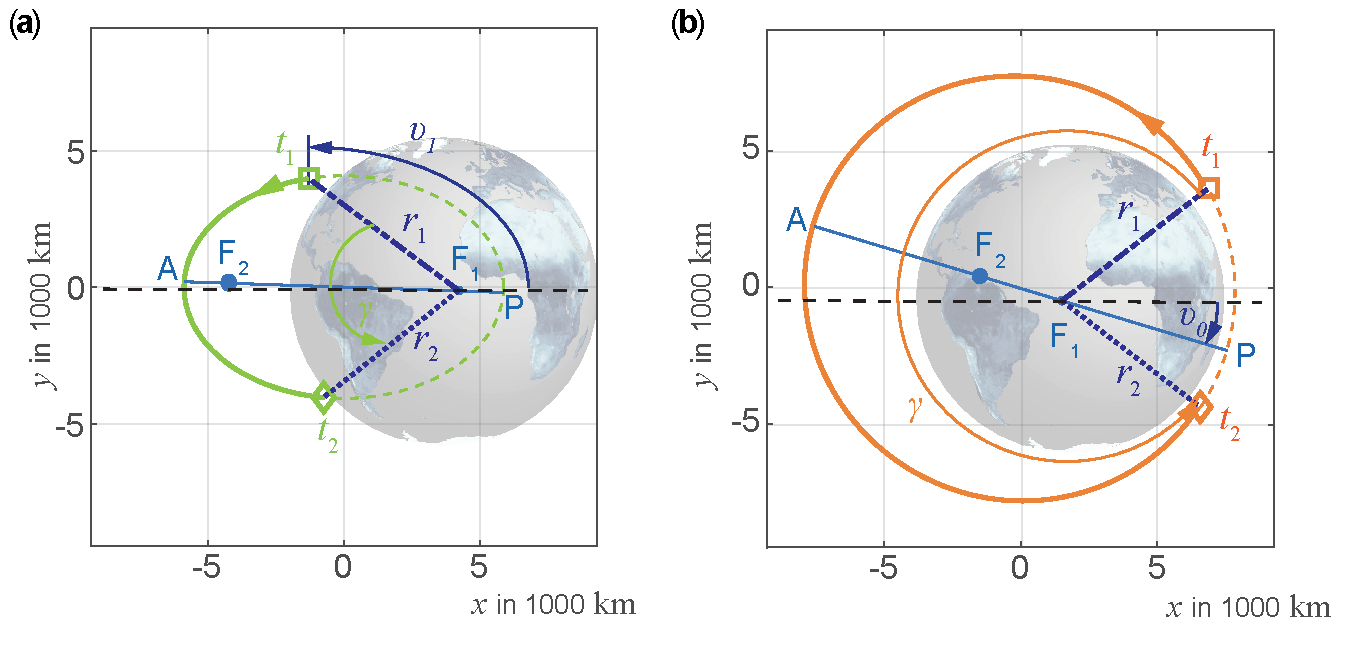
\includegraphics[width=\textwidth]{LambertProblem01Loesung.pdf} 
	\caption[L�sung des Lambert-Problems.]{L�sung des Lambert-Problems f�r das Beispiel des Abfangens einer interkontinentalen ballistischen Rakete durch eine Raumsonde im Schwerefeld der Erde. \fa Parameter: $r_1 = \SI{6800}{\kilo\metre},\, r_2 = \SI{6400}{\kilo\metre},\, \gamma=75\degree,\ t_\text{F}^*=3000s = \SI{50}{\minute}$. Es ergibt sich die gr�ne Ellipse mit Parametern $p = \SI{2831}{\kilo\metre},\, \e=0.7195,\, \eta = -1.7\degree$. \fb Mit gleichen Anfangsvektoren aber unterschiedlichem eingeschlossenen Winkel $\gamma=285\degree=360\degree- 75\degree$  ergibt sich die l�ngere orangefarbene Ellipse mit einer Flugzeit $t_\text{F}^*=6000s = \SI{100}{\minute}$ und Ellipsenparametern von: $p = \SI{7589}{\kilo\metre},\, \e=0.1988,\, \eta = -16.7\degree$. (\mscr~ \mladynref{LambertProblem01.m} nach \cite{Gatland2022}.)
	}
	\label{abb:adyn_lambert_bsp}
\end{figure}
Wir haben in der gezeigten Rechnung eine eindeutige L�sung erhalten. Das ist bei Randwertaufgaben jedoch keinesfalls immer der Fall, wie wir in \probref{adyn_manoevers4} zeigen werden. Bei ung�nstig gew�hltem Startwert $p^{(0)}$ kann es sein, dass die Itration nicht konvergiert. Es empfiehlt sich daher, sich mit einer numerischen Vorw�rtsrechnung eine Tabelle von $p^{(i)}$ und den zugeh�rigen $t_\text{F}^{(i)}$ zu beschaffen. 

F�r die Bahnberechnung in der Astrodynamik braucht man h�ufig auch die Geschwindigkeiten bei den jeweiligen normalen Anomalien, insbesondere bei $\upsilon_1$ und $\upsilon_2$. Diese berechnen sich nach \cite{Gatland2022}:
\begin{align}
    \vec{v}_\text{tr} = \sqrt{\frac{\mu}{p}}\,\lek e\,\sin\upsilon\,\vec{e}_\text{r} + \lk 1 + e \,\cos\upsilon \rk \,\vec{e}_\upsilon \rek \,,\label{eq:adyn_lambert08}
\end{align}
worin $\vec{e}_r$ \bzw $\vec{e}_\upsilon$ Einheitsvektoren sind. In \probref{adyn_manoevers4} werden wir noch eine andere Berechnung f�r die Geschwindigkeiten zeigen.\\ 
F�r das Lambert-Problem gibt es wie erw�hnt zahlreiche Anwendungen. Beispielsweise ist die Berechnung der Bahn eines Transportraumschiffs zur ISS nach dem \gls{Brennschluss} des Triebwerks der Startrakete ein Lambert-Problem, ebenso wie die Planung und Berechnung eines optimalen Startzeitpunkts (Start-Fensters) zum Mars \bzw zur Venus (\probref{adyn_manoevers5}).
In \probref{adyn_manoevers6} behandeln wir das Abfangen einer interkontinentalen ballistischen Rakete.

\subsection{Man�ver mit kontinuierlichem Schub}\label{kap:adyn_kont_maneuver}

Wir wollen uns nun Man�ver mit kontinuierlichem Schub anschauen, wie sie \zb durch Plasma- oder Ionenstrahltriebwerke oder allgemein elektrische Antriebe realisiert werden k�nnen. Diese Triebwerke sind wieder verst�rkt in das Interesse der Raumfahrt ger�ckt, beispielsweise bei der Raumsonde BepiColombo im Jahr 2018 \cite{Althaus2007, Krueger2018, Messerschmid2017}.\\
Im Gegensatz zu einem chemischen Antrieb auf Basis von Verbrennung von Treibstoff, steht beim elektrischen Antrieb quasi kontinuierlich und �ber Solarpanele auch nahezu unbegrenzt  Energie zur Verf�gung, allerdings ist die Leistung (Energie pro Zeit) begrenzt. Ein Vorteil der elektrischen Antriebe ist aber, dass die Aussto�geschwindigkeit der Teilchen (beschleunigte Ionen) mit bis zu $v_1= \SI{50}{\km\per\second}$ deutlich �ber den Werten von chemischen Triebwerken ($v_\text{G}\approx 3 \ldots 5\,\SI{}{\km\per\second}$) liegt. Damit ist pro $\SI{}{\kg}$ Treibstoffmasse auch ein etwa $10$ mal gr��erer Schub verbunden. Dennoch gibt es zwei Nachteile, 
\begin{itemize}
    \item zum einen funktionieren Ionenstrahltriebwerke nicht unter Atmosph�renbedingungen, was ihren Einsatz auf h�here Orbits und interplanetare Fl�ge begrenzt und
    \item wegen der begrenzten elektrischen Leistung sind zum anderen nur sehr kleine Sch�be im Bereich von $\SI{1e-3}{\newton}$ bis etwa $\SI{0.5}{\newton}$ m�glich. 
\end{itemize}
Damit sind auch die Einsatzbereiche der Triebwerke vorgezeichnet.\\
Wir wollen uns als ein Beispiel den Flug von einer nahen Erdumlaufbahn (\zb LEO) zu einem geostation�ren Orbit (GEO) mit einem Ionentriebwerk durch sogenanntes Aufspiralen im Vergleich zum Hohmann-Transfer (\kap{adyn_hohmann_transfer}) anschauen.
In der Bewegungsgleichung f�r kontinuierliche Sch�be soll die sich �ber die Man�verzeitdauer ver�ndernde Gravitationskraft $\vec{F}_\text{G}$ ber�cksichtigt werden. Alle anderen wirkenden Kr�fte sollen weiterhin vernachl�ssigt werden. Wir haben also f�r das Raumschiff (Masse $m_\text{R}$) mit kontinuierlichem Triebwerk folgende Bewegungsgleichung:
\begin{align}
    \ddot{\vec{r}} = \dot{\vec{v}} = \frac{\vec{F}_\text{S}\lk t\rk}{m_\text{R}(t)} +\frac{\vec{F}_\text{G}\lk\vec{r}\rk}{m_\text{R}(t)}\,.\label{eq:adyn_ionentr_01}
\end{align}
Im Allgemeinen wird man diese Gleichung nur numerisch l�sen k�nnen (\probref{adyn_manoevers7}), wir k�nnen aber mit zwei Annahmen eine gute analytische N�herung herleiten.
Es gilt zum einen, dass $|\vec{F}_\text{S}| \ll |\vec{F}_\text{G}|$ und zum anderen soll der Schub immer tangential zur Bahn, also parallel zur Geschwindigkeit erfolgen, also:
\begin{align}
    \vec{F}_\text{S}\,\vec{v}_\text{R} = F_\text{S}\,v_\text{R}\,. \label{eq:adyn_ionentr_02}
\end{align}
Das bedeutet auch, dass die Bahn w�hrend des gesamten Man�vers als kreis�hnlich betrachtet werden kann, das Aufspiralen wird also mit sehr kleinen H�hen�nderungen pro Zeit (\bzw Umlauf) verbunden sein. Man muss dann nat�rlich bei der Rechnung aufpassen, dass die Bedingungen f�r die gemachten N�herungsannahmen noch erf�llt sind. Wir benutzen die  Gleichung f�r die Gesamtenergie \eqref{eq:hm_vis-viva} und die \gls{visvivaadyn} \eqref{eq:hm_vis-viva}, die wir etwas umformen und beide nach der Zeit ableiten:
\begin{align}
\begin{split}
    \frac{\D }{\D t}\,H = \frac{\D }{\D t} \lk -\frac{\mu_\text{E}}{2a}\rk &= \frac{\D}{\D t}\lk\frac{1}{2}\,v^2 - \frac{m_\text{E}\,G}{r} \rk %= \frac{\D}{\D t} \lk\frac{1}{2}\,\vec{v}^2-\frac{\mu_\text{E}}{r}\rk 
		= \frac{\D}{\D t}\lk \frac{1}{2}\,\vec{v}^2 + U\lk r\rk \rk\\
    &=\vec{v}\,\frac{\D \vec{v}}{\D t} + \frac{\d U\lk r\rk}{\d \vec{r}}\,\frac{\D \vec{r}}{\D t}= \vec{v}\,\lk\frac{\D \vec{v}}{\D t} - \vec{g}\lk r \rk \rk \,.
\end{split} \label{eq:adyn_ionentr_03}
\end{align}
Hier haben wir die spezifische (auf die Masse bezogene) potentielle Energie 
\begin{align}
    U\lk r\rk = \frac{1}{m_\text{r}}\,\int\limits_r^\infty F_\text{G}\lk r\rk\, \D r  \label{eq:adyn_ionentr_04}
\end{align}
und die Gravitationsbeschleunigung 
\begin{align}
    \vec{g} = \frac{\vec{F}_\text{G}}{m_\text{r}} = - \frac{\d}{\d \vec{r}}\,U\lk r\rk = -\vec{\nabla}\,U\lk r\rk \label{eq:adyn_ionentr_05}
\end{align}
benutzt. 
%Gleichung \eqref{eq:adyn_ionentr_03} ist aber nach \eqref{eq:hm_bewgl1} gleich der zeitlichen Ableitung der Gesamtenergie, also:
%\begin{align}
    %\frac{\D }{\D t} = \lk -\frac{\mu_\text{E}}{2a}\rk = \frac{\D }{\D t}\,H\,. \label{eq:adyn_ionentr_06}
%\end{align}
Damit k�nnen wir \eqref{eq:adyn_ionentr_03} mit \eqref{eq:adyn_ionentr_01} schreiben:
\begin{align}
    \frac{\D}{\D t}\, H = \vec{v}\,\lk \frac{\vec{F}_\text{S}}{m_\text{R}} + \vec{g} - \vec{g} \rk = \vec{v}\,\frac{\vec{F}_\text{S}}{m_\text{R}} ~~~~ \rightarrow ~~~~ \frac{1}{v}\,\frac{\D}{\D t}\,H = \frac{F_\text{S}}{m_\text{R}}\,.\label{eq:adyn_ionentr_07}
\end{align}
Das ist unsere Bewegungsgleichung. Die bereits gemachte Annahme f�r kleine Sch�be f�hrt zu kreis�hnlichen Bahnen, die wir durch
\begin{align}
    v = \left|r \dot{\varphi} \vec{e}_\varphi \right| = \sqrt{\frac{G\,m_\text{E}}{r}} = \sqrt{\frac{\mu_\text{E}}{r}}~~~~ \text{und} ~~~~ H =-\frac{G\,m_\text{E}}{2r}= -\frac{\mu_\text{E}}{2r} \label{eq:adyn_ionentr_08}
\end{align}
ausdr�cken (siehe auch \kap{hm_abl_kepler}). \\
Damit erhalten wir:
\begin{align*}
    \frac{1}{2}\,\sqrt{\frac{\mu_\text{E}}{r^3}}\,\frac{\D r}{\D t} = \frac{F_\text{S}}{m_\text{R}}
\end{align*}
und durch Integration
\begin{align}
\begin{split}
    \frac{\sqrt{\mu_\text{E}}}{2}\,\int\nolimits_{r_1\approx R_\text{E}+h}^{r_2} r^{-\frac{3}{2}}\,\D r = &-\sqrt{\mu_\text{E}}\,\lk \frac{1}{\sqrt{r_2}} - \frac{1}{\sqrt{r_1}}\rk = \int\nolimits_{t=0}^{t_\text{end}}\,\frac{F_\text{S}}{m_\text{R}}\,\D t = \Delta v_\text{kont}\\
    \rightarrow ~~~~ &\Delta v_\text{kont} = \sqrt{\frac{\mu_\text{E}}{r_1}}\,\lk 1-\sqrt{\frac{r_1}{r_2}}\rk = v_1-v_2 \,.
\end{split} \, \label{eq:adyn_ionentr_09}
\end{align}
Beim kontinuierlichen Schub ist also der Geschwindigkeitsbedarf durch die Differenz der Umlaufgeschwindigkeiten in der Anfangs- und Endbahn gegeben. \\
Vergleichen wir das mit dem Hohmann-Transfer \eqref{eq:adyn_hohmann04}
\begin{align}
    \Delta v_\text{Hohmann}=  v_\text{P}-v_\text{A} +v_2-v_1 = v_\text{P}-v_\text{A} -\Delta v_\text{kont}\,, \label{eq:adyn_ionentr_10}
\end{align}
so sehen wir, dass beim kontinuierlichen Schub ein h�herer Energiebetrag notwendig ist (\figref{adyn_Ionenantrieb01}a). \\
Wir wollen noch die Flugzeit unter der Annahme konstanten Schubs und konstanter Massenverlustrate $\dot{m}_\text{R}$ (das sind im wesentlichen die ausgesto�enen Ionen) berechnen. Aus \eqref{eq:adyn_ionentr_07} folgt dann mit $m\lk t\rk = m_0 - \dot{m}_\text{r}\lk t-t_0\rk$:
\begin{align*}
    \int\limits_{t_0}^t\frac{F_\text{S}}{m\lk t \rk} \,\D t = \frac{F_\text{S}}{m_0}\,\int\limits_{t_0}^t \, \frac{\D t'}{1-\frac{\dot{m}_\text{R}}{m_0}\,\lk t'-t_0 \rk} = \frac{F_\text{S}}{\dot{m}_\text{R}} \,\ln \,\lek 1-\frac{\dot{m}_\text{R}}{m_0}\,\lk t-t_0\rk\rek
\end{align*}
\begin{align*}
    \rightarrow ~~~~ \frac{r}{r_1} = \lek 1 + \sqrt{\frac{r_1}{\mu_\text{E}}}\,\frac{F_\text{S}}{\dot{m}_\text{R}}\,\lk \ln \lek 1-\frac{\dot{m}_\text{R}}{m_0}\,\lk t-t_0\rk\rek\rk\rek \;. 
\end{align*}
Wir haben die Zeiten f�r den Flug zum GEO mit kontinuierlichem Antrieb in \figref{adyn_Ionenantrieb02} dargestellt und mit denen f�r einen �quivalenten Hohmann-Transfer verglichen.
Man erkennt, dass bei kontinuierlichen (elektrischen) Triebwerken mit deutlich l�ngeren Flugzeiten zu rechnen ist. Deswegen kommt es bei Raketenantrieben immer zu einer Kombination von chemischen Triebwerken (schon f�r den Start von der Erde notwendig) und elektrischen Triebwerken. Wir wollen nochmals explizit darauf hinweisen, dass die N�herungsannahmen, die wir weiter oben gemacht haben, nicht mehr f�r die gesamte Flugzeit erf�llt sind. Das kann man auch am starken Anstieg der Kurve $r(t)$ am Ende der Flugzeit sehen. Eine detaillierte numerische Rechnung ist Gegenstand von \probref{adyn_manoevers7}. In \probref{adyn_manoevers8} wollen wir dann auch den Flug mit einem kontinuierlichen Antrieb zum Mars aus einer Parkbahn um den Mond heraus betrachten und die Gleichung \eqref{eq:adyn_ionentr_01} numerisch l�sen. Es sei darauf hingewiesen, dass auch der Strahlungsdruck (siehe \kap{adyn_strahlungsdruck}) besonders im interplanetaren Raum zum kontinuierlichen Antrieb benutzt werden. Dazu werden Raumschiffe mit sogenannte Sonnensegeln ausgestattet. In \cite{Bailer2021} wird die japanische Mission IKAROS behandelt, die mit einem solchen Antrieb im interplanetaren Raum unterwegs ist. 

\begin{figure}[H]
	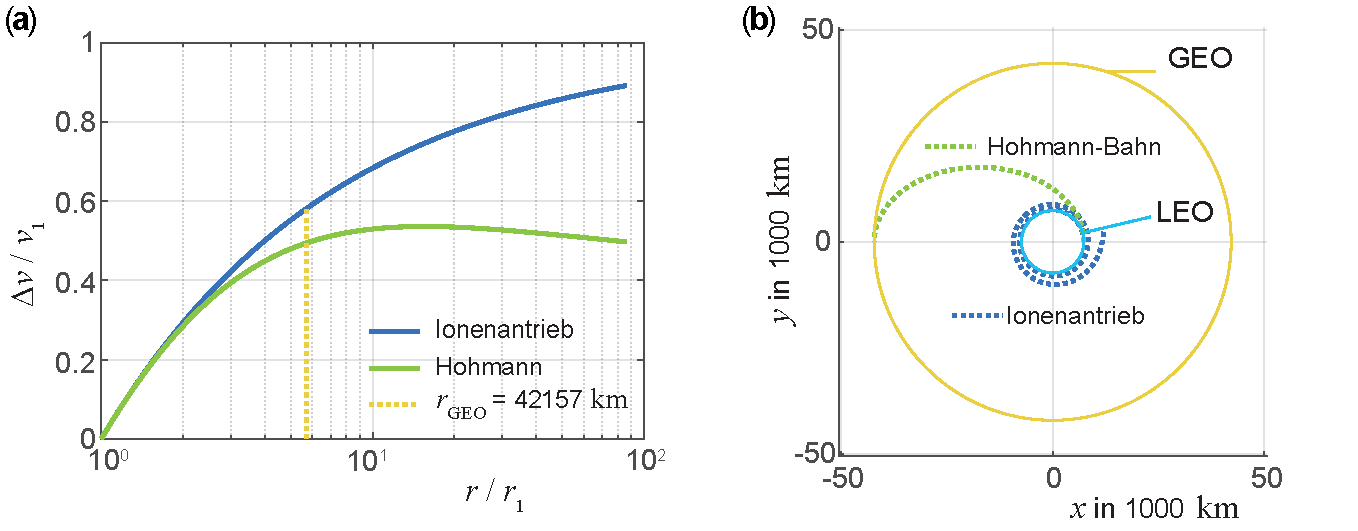
\includegraphics[width=\textwidth]{Ionenantrieb01.pdf} 
	\caption[Ionenantrieb im Vergleich zu Hohmann-Transfer.]{Ionenantrieb im Vergleich zu einem Hohmann-Transfer. \fa Geschwindigkeitsbedarf f�r Transfer von $r_1$ nach $r_2$. \fb Bahnform. Parameter: $r_1= \SI{1000}{\km} + R_\text{E}$, $r_2 = \SI{35786}{\km} + R_\text{E}$, Schub $F_\text{S}= \SI{0.5}{\newton}$, Anfangsmasse $m_0= \SI{10000}{\kg}$, Massenaussto� $\dot{m}_\text{R} = \SI{3e-3}{\kg\per\second}$. }
	\label{abb:adyn_Ionenantrieb01}
\end{figure}

\begin{figure}[H]
	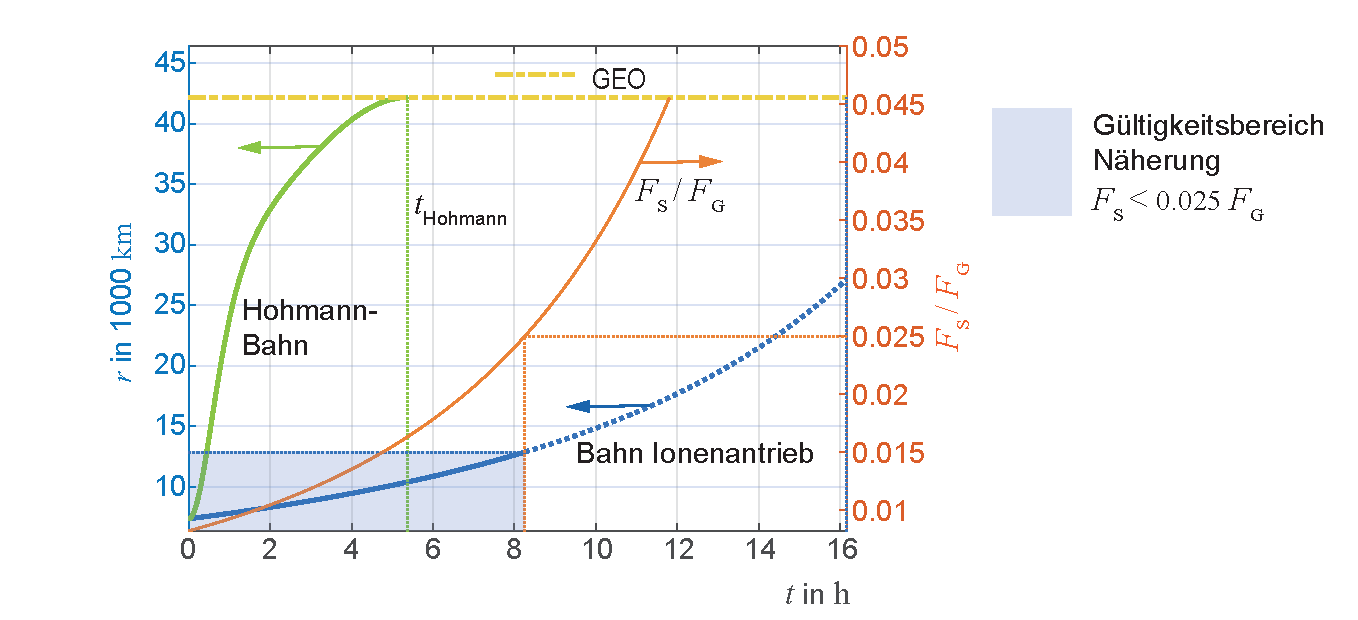
\includegraphics[width=\textwidth]{Ionenantrieb02.pdf} 
	\caption[Abstand zur Erde und Flugzeit bei Flug zu geostation�rem Orbit.]{Abstand zur Erde und Flugzeit bei einem Flug zu einem geostation�ren Orbit mit Ionenantrieb im Vergleich zu einem Hohmann-Transfer.}
	\label{abb:adyn_Ionenantrieb02}
\end{figure}


\subsection{Gravity-Assist-Man�ver}\label{kap:adyn_gravity_assist}

Wir wollen nun die ebenfalls sehr wichtigen \glslink{GA}{\textit{Gravity-Assist-Man�ver (GA-Man�ver)}}\index{Gravity-Assist-Man�ver} behandeln, denen wir bereits unter dem Namen Swing-By\index{Swing-By-Man�ver}\footnote{Wir benutzen die Begriffe GA-Man�ver und Swing-By-Man�ver synonym. H�ufig wird auch die Schreibweise Swingby oder Flyby verwendet.} im Kapitel 1 von Band I und auch im Kapitel Himmelsmechanik begegnet sind. 
Warum ist das Gravity-Assist-Man�ver f�r die Raumfahrt insbesondere zu den weiter entfernten Planeten so bedeutsam? Der Hohmann-Transfer erfordert bei entfernt liegenden Planeten sehr gro�e Geschwindigkeitsbudgets und f�hrt auch zu sehr langen Flugzeiten. So br�uchte man nach \eqref{eq:adyn_hohmann04} f�r einen Hohmann-Transfer zum Jupiter bereits ein $\Delta v \approx \SI{14}{\km\per\second}$, was zumindest bei der derzeitigen Raketentechnologie zu v�llig unakzeptablen, \dh verschwindenden, Nutzlasten f�hren w�rde.\\ 

\begin{figure}[H]
	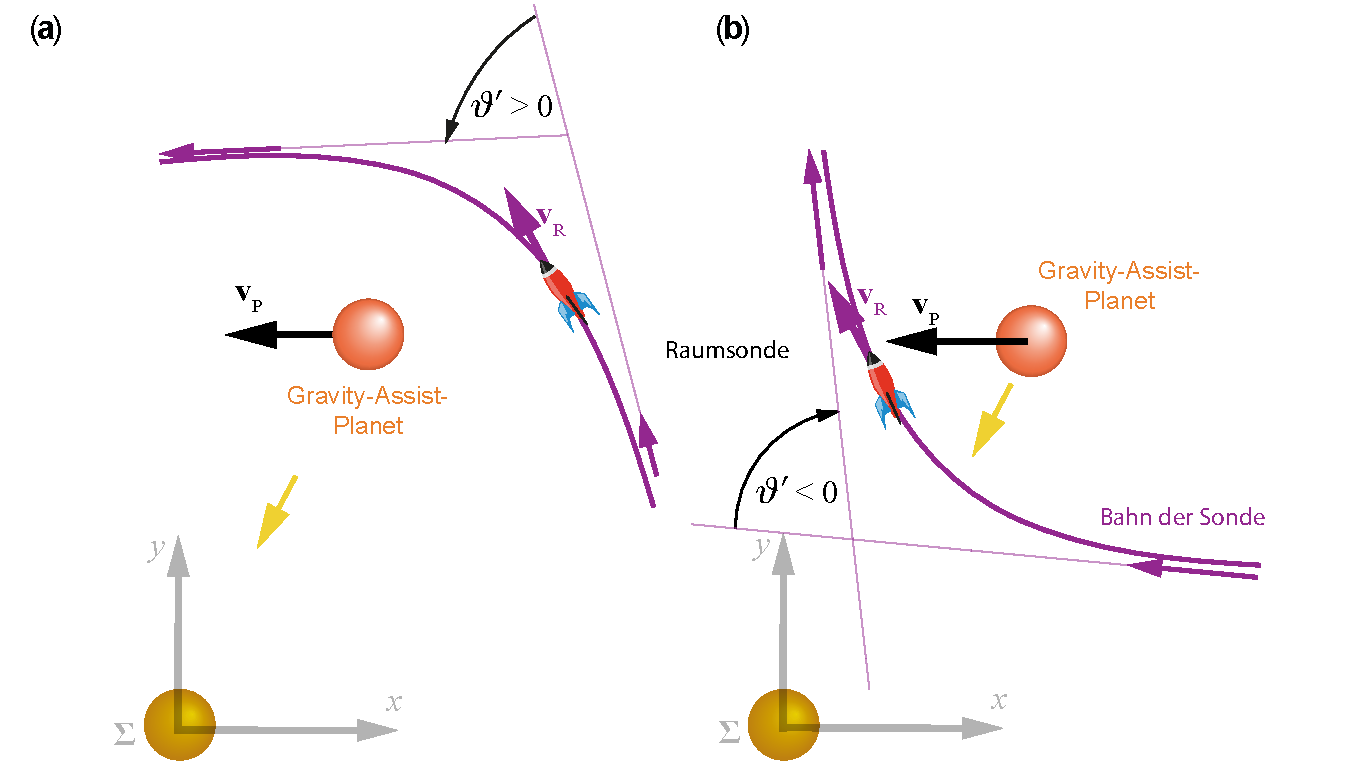
\includegraphics[width=\textwidth]{GravityAssistManoever01.pdf} 
	\caption[Verschiedene Swing-By-Man�ver im heliozentrischen \KOS .]{Swing-By-Man�ver im heliozentrischen Koordinatensystem. \fa Bahn der Sonde liegt "`hinter"' dem Planeten, die Ablenkung erfolgt entgegen dem Uhrzeigersinn ($\vartheta' >0$). \fb Bahn der Sonde liegt "`vor"' dem Planeten, die Ablenkung erfolgt im Uhrzeigersinn ($\vartheta' < 0$).}
	\label{abb:adyn_swingby00}
\end{figure}

Erst mit den Swing-By-Man�vern wurden solche interplanetaren Raumfl�ge wirklich m�glich. Erw�hnenswert ist, dass die Entdeckung des Swing-By 1961 von dem Mathematik-Studenten Michael Minovitch\footnote{Michael Minovitch (geb. 1935) ist ein US-amerikanischer Mathematiker, der als erster gezeigt hat, dass die Bahnen von Raumsonden beim Vorbeiflug an Planeten durch ein Swing-By-Man�ver Geschwindigkeit hinzugewinnen k�nnen.}\indexp{Minovitch, Michael Andrew} w�hrend seines studentischen Praktikums am \textit{\gls{jpladyn}~(JPL)}\index{Jet Propulsion Lab (JPL)} in Pasadena (Kalifornien) gemacht wurde. Innerhalb der NASA und der ESA wird auch Giuseppe Colombo\footnote{Giuseppe Colombo (1920--1984) war ein italienischer Ingenieur und Mathematiker, der auf den Gebieten der theoretischer Mechanik, insbesondere der Schwingungs- und Himmelsmechanik und der Astrodynamik t�tig war. Neben seinen Beitr�gen zum Swing-By ist auch seine Konzeptentwicklung des Space Tethers (Weltraumfahrstuhl, siehe auch �bung im Kapitel 1, Band I)\indexp{Colombo, Giuseppe} erw�hnenswert.} als konzeptioneller Kopf und genialer Weiterentwickler von Swing-By-Man�vern genannt.\\
Wie kann eine Raumsonde durch ein GA-Man�ver an einem Planeten an Geschwindigkeit gewinnen? Wir hatten im Kapitel Streuprobleme (Band I, Kapitel  1.3.5) gesehen, dass es sich bei Swing-By-Man�vern um ein elastisches Streuproblem im Gravitationsfeld des Planeten handelt. Die Bewegung einer Sonde um den sogenannten Gravity-Assist-Planeten erfolgt auf einer Hyperbelbahn und nat�rlich bleibt bei diesem elastischen Streuprozess die Gesamtenergie des Systems erhalten. Es findet aber eine Energie�bertragung $\Delta T$ zwischen Planet und Raumsonde statt, die im heliozentrischen \KOS\ zu einer Geschwindigkeits�nderung der Sonde f�hrt. Das GA-Man�ver ist im reinen Zweik�rperproblem nicht erkl�rbar, denn es muss die heliozentrische Geschwindigkeit des Planeten f�r die Erkl�rung des Energie- \bzw Geschwindigkeits�bertrags ber�cksichtigt werden.\footnote{In der Referenz \cite{Walter2018} wird eine sch�ne Analogie f�r den Swing-By gegeben. Nach dieser kann eine Raumsonde mit einem Roller-Skater verglichen werden. Der Roller-Skater h�ngt sich f�r eine kurze Zeit an einem vorbeifahrenden Bus (den Planeten), l�sst diesen dann nach einiger Zeit wieder los und hat damit Geschwindigkeit gewonnen. Das Festhalten entspricht der Gravitationskraft zwischen Planet und Raumsonde.} Man behandelt deshalb das Problem des Swing-By in einer Abfolge von Schritten, zun�chst im heliozentrischen, dann im planetaren und zum Schluss wieder im heliozentrischen System, in dem dann ja auch der Geschwindigkeitsgewinn beobachtet wird.\\

\begin{figure}[H]
	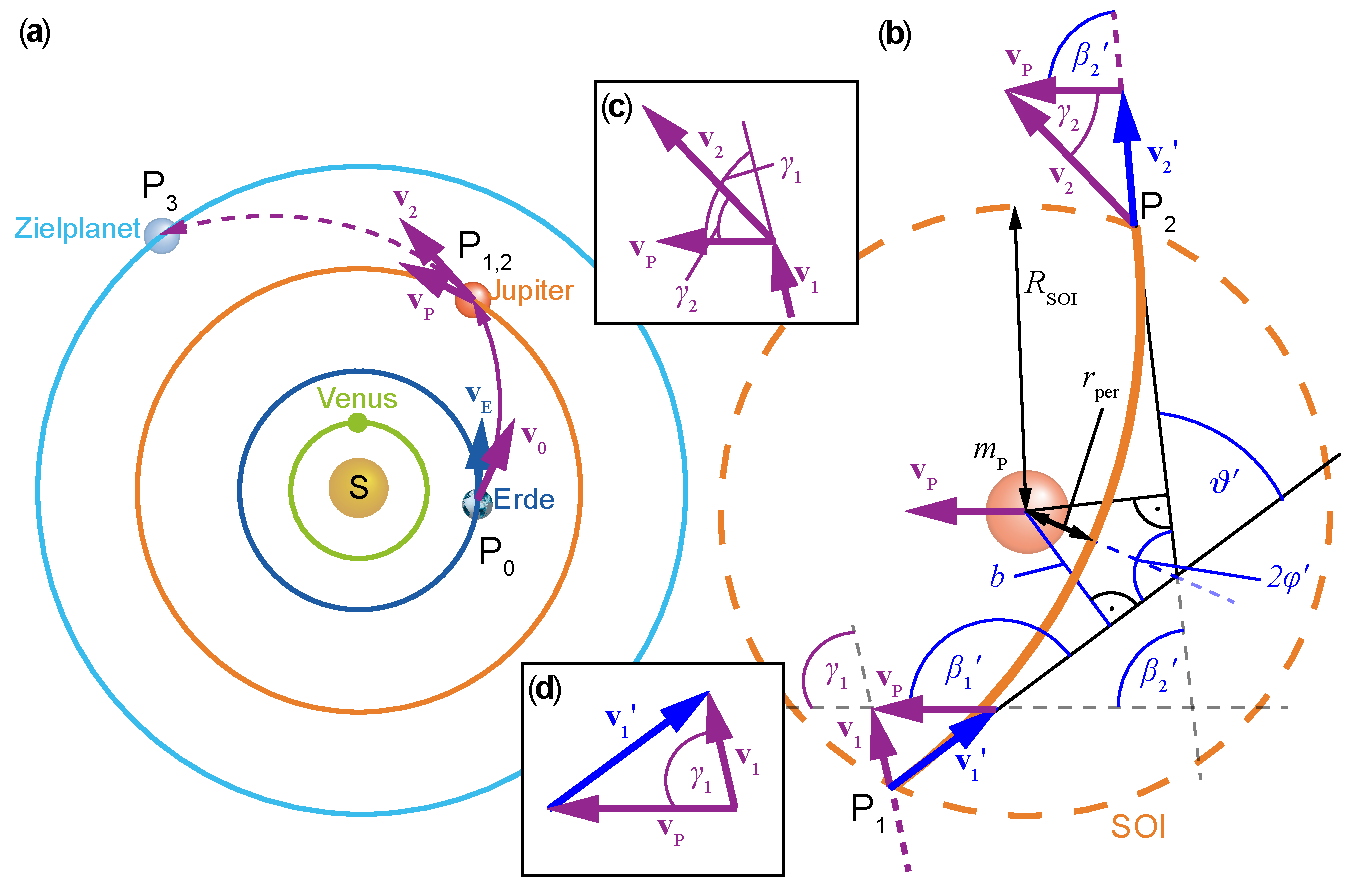
\includegraphics[width=\textwidth]{SwingByHeliozPlanetoz.pdf} 
	\caption[Swing-By-Man�ver im heliozentrischen und planetaren \KOS .]{Swing-By-Man�ver im heliozentrischen \fa und im planetaren \KOS\ \fb im Bereich der Einflusssph�re (SOI). Wir haben hierbei auch f�r die weiteren Darstellungen folgende Konventionen gew�hlt: Gr��en im heliozentrischen \KOS\ sind ungestrichen (\zb $\vec{v}_1,\, \gamma_1$) und in der Farbe lila dargestellt, w�hrend Gr��en im planetaren \KOS\ dagegen gestrichen (\zb $\vec{v}_1{}',\,\beta_1{}'$) und in den Farben blau oder orange angegeben sind. Systemunabh�ngige Gr��en sind ungestrichen (\zb $r_\text{per},\, R_\text{SOI}$) und in der Farbe schwarz dargestellt. Die Inlets zeigen \fc die Geschwindigkeitsverh�ltnisse am Eintrittspunkt in die SOI des Planeten \bzw \fd die Gesamt�nderung des heliozentrischen Geschwindigkeitsvektors der Raumsonde.}
	\label{abb:adyn_swingby01}
\end{figure}

Wir wollen uns die mathematische Behandlung des Swing-By-Man�vers etwas vereinfachen, indem wir annehmen, dass alle Bewegungen in der Ebene der Ekliptik stattfinden. 
Bei der Streuung am Planeten wird die Raumsonde um einen zun�chst noch nicht bekannten Winkel $\vartheta'$ abgelenkt. Dabei kann der Winkel sowohl negativ (Richtungs�nderung entgegen dem Uhrzeigersinn) als auch positiv (Richtungs�nderung im Uhrzeigersinn) sein, siehe \figref{adyn_swingby00}, je nachdem, ob sich die Sonde "`vor"' oder "`hinter"' dem Planeten (von der Sonne aus betrachtet) an diesem vorbei bewegt. Gleiches gilt f�r die Geschwindigkeits�nderung.\\ 
\figref{adyn_swingby01}a zeigt das Gravity-Assist-Man�ver im heliozentrischen \KOS\ und \figref{adyn_swingby01}b im \KOS\ des Gravity-Assist-Planeten, welches wegen der gro�en Masse $m_\text{P} \gg m_\text{R}$ zugleich das Schwerpunktsystem ist. Mit den Bezeichnungen aus den Abbildungen finden wir f�r die Situation am Punkt $\text{P}_1$ vor dem Swing-By-Man�ver, \dh vor der Streuung (\figref{adyn_swingby01}c):
\begin{subequations}
    \begin{align}
        \vec{v}_1{}' &= \vec{v}_1 - \vec{v}_\text{P}\,, \label{eq:adyn_swingby01a} \\
        {v_1{}'}^2 &= v_1{}^2 + v_\text{P}{}^2 - 2\,v_1\,v_\text{P}\,\cos\gamma_1\,.\label{eq:adyn_swingby01b} 
    \end{align} \label{eq:adyn_swingby01} 
\end{subequations}
Hierbei haben wir unterstellt, dass wir in der sogenannten \gls{SOI} (englisch \textit{Sphere of Influence} (SOI))\index{Einflusssph�re}\index{Sphere of Influence (SOI)} des Gravity-Assist-Planeten (in \figref{adyn_swingby01}b als gestrichelter Kreis gezeichnet) nur die Gravitationskraft des Gravity-Assist-Planeten ber�cksichtigen m�ssen\footnote{Die Berechnung der Gr��e der \gls{SOI} (SOI) ist nicht ganz einfach, h�ufig finden sich in der Literatur auch nicht ganz korrekte Definitionen und Berechnungen f�r die SOI. Wir geben die Werte f�r die Radien der SOI der einzelnen Planeten am Ende dieses Kapitels in Tabelle \ref{tab:adyn_results_swingby} an und empfehlen \probref{adyn_SOI}, in der wir die korrekte Beziehung herleiten.}.

\begin{figure}[H]
	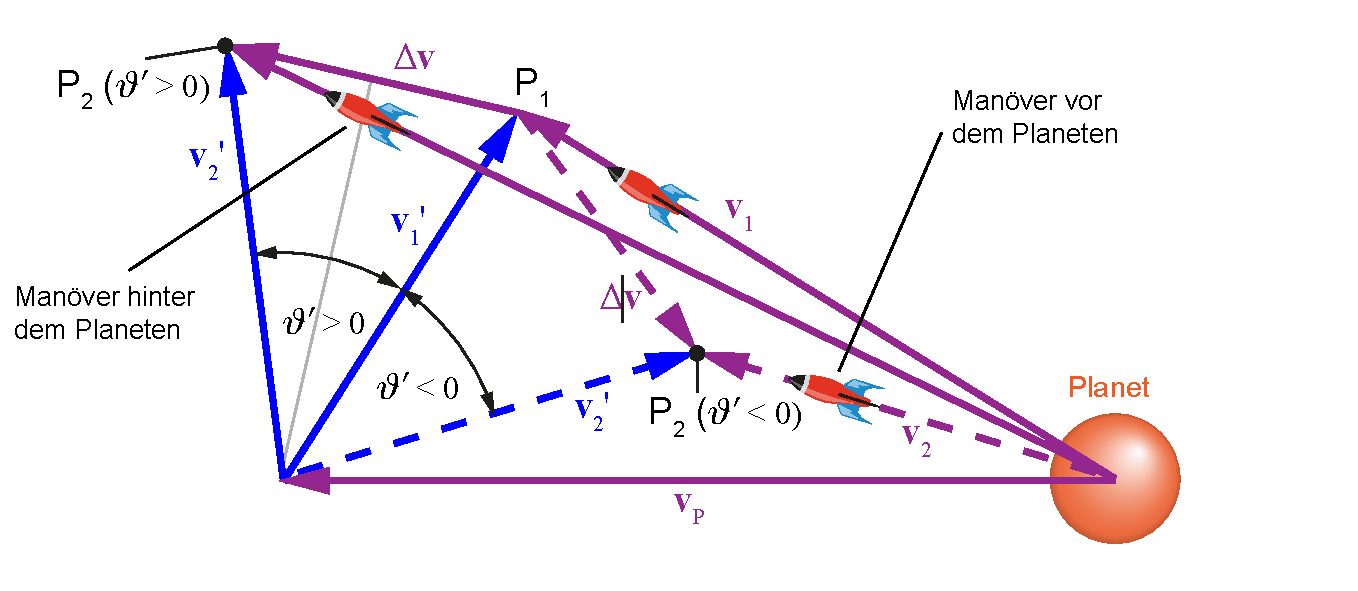
\includegraphics[width=\textwidth]{FlyByVorHinterPlanet.pdf} 
	\caption[Vektordiagramm der Geschwindigkeiten beim Swing-By-Man�ver.]{Vektordiagramm der Geschwindigkeiten beim Swing-By-Man�ver. Die Darstellung ist eine Kombination der beiden Teilzeichnungen \figref{adyn_swingby01}c,d f�r die jeweiligen F�lle des GA-Man�vers "`vor"' \bzw "`hinter"' dem Planeten.}
	\label{abb:adyn_swingby01a}
\end{figure}

Wegen Energieerhaltung beim elastischen Sto� gilt
\begin{align}
    v_1{}' = v_2{}' = v_\infty{} \,, \label{eq:adyn_swingby02} 
\end{align}
worin wir die asymptotische Geschwindigkeit in der Streuhyperbel mit $ v_\infty{}$ bezeichnet haben. Au�erhalb der SOI wird der Einfluss der Gravitation des Planeten gegen�ber der Gravitation der Sonne vernachl�ssigt, so dass am Punkt $\text{P}_2$ (\vgl \figref{adyn_swingby00}b) f�r die Geschwindigkeit $\vec{v}_2$ dann im heliozentrischen System wieder gilt:
\begin{subequations}
    \begin{align}
        \vec{v}_2 &= \vec{v}_2{}' + \vec{v}_\text{P} \,, \label{eq:adyn_swingby03a} \\
        v_2{}^2 &= {v_\infty{}}^2 + v_\text{P}{}^2 - 2\,v_\infty{}\,v_\text{P}\,\cos(180\degree - \beta_2{}') = {v_\infty{}}^2 + v_\text{P}{}^2 + 2\,v_\infty{}\,v_\text{P}\,\cos\beta_2{}'\,. \label{eq:adyn_swingby03b} 
    \end{align} \label{eq:adyn_swingby03} 
\end{subequations}
Man erkennt schon an den Gleichungen \eqref{eq:adyn_swingby01b} und \eqref{eq:adyn_swingby03b}, dass ein Geschwindigkeitsgewinn $\Delta v = v_2-v_1$ mit der Geschwindigkeit der Bewegung des Gravity-Assist-Planeten $v_\text{P}$ zusammenh�ngt. Dies ist in \figref{adyn_swingby01a} f�r die beiden F�lle $\vartheta' >0$ und $\vartheta' <0$ verdeutlicht.\\
Wir wollen nun diesen Geschwindigkeitsgewinn nach folgendem Schema berechnen:
\begin{enumerate}[1.]
	\item \textit{Berechnung der Anflugbedingungen im heliozentrischen System}\\ 

	Die als bekannt angenommenen Anflugbedingungen sind die heliozentrische Geschwindigkeit der Raumsonde $\vec{v}_1$, die Bahngeschwindigkeit $\vec{v}_\text{P}$ des Planeten, dessen Masse $m_\text{P}$ und der kleinste Abstand $r_\text{per}$ (periplanetarer Abstand), den die Raumsonde im Vorbeiflug am Planeten erreichen kann. Letzterer entspricht dem Perizentrumsabstand\index{Perizentrum} der Streuhyperbel. Dar�ber hinaus seien noch die Vektoren $\vec{r}_\text{R}$ und $\vec{r}_\text{P}$ bekannt.
	Aus den Vektorwerten $\vec{v}_1$ und $\vec{v}_\text{P}$ berechnen sich die Betr�ge $v_1,\,v_\text{P}$ und der Winkel $\gamma_1{}$.\\
	
	\item \textit{�bergang ins planetare System und Berechnung des Streuwinkels}\\ 
	
	�ber Gleichung \eqref{eq:adyn_swingby01} berechnet man $v_1{}'=v_\infty{}$ und $\gamma_1{}$. 
	Nun muss der Streuwinkel~$\vartheta'$ bestimmt werden. % f�r den nach \figref{adyn_swingby01} die Beziehung $\vartheta' = 180\degree-2\varphi'$ gilt. 
	Hier k�nnen  die Ergebnisse aus der Behandlung der Rutherford-Streuung\index{Streuung,!Rutherford-} im Kapitel Streuprobleme (Band I, Kapitel  1.3.5) benutzt werden, da wegen $m_\text{P} \gg m_\text{R}$ das planetare System auch gleichzeitig das Schwerpunktsystem f�r die Streuung der Raumsonde am Planeten ist. Den Streuwinkel f�r das Zentralkraftfeld hatte wir dort mit Formel (1.80) wie folgt berechnet:
	\begin{align}
		\sin^2\lk \frac{\vartheta'}{2} \rk & \:=\: \frac{1}{1 + 4 E^2 b^2/\alpha^2}\,, \label{eq:adyn_StreuungVglBew}
	\end{align}
	worin $E$ die Energie des einfallenden Streuteilchens, $\alpha$ die St�rke des Zentralkraftfeldes (dort war es ein Coulomb-Feld) und $b$ der Streuparameter waren. Nun m�ssen die �quivalenten Gr��en f�r das Swing-By-Man�vers im Gravitationsfeld berechnet werden.
	Da hier mit auf die Masse der Raumsonde bezogenen Gr��en gerechnet wird, ergibt sich mit der Masse $m_\text{P}$ des Gravity-Assist-Planeten f�r die Energie $H$ \bzw $\alpha$ :
	\begin{align}
	\begin{split}
 		H &= \frac{v_\infty{}^2}{2} ~~~~ (\text{f�r} ~~~~ r\to \infty \,~~~ \text{vgl.}~\eqref{eq:hm_bewgl1})\,, \\ 
		\alpha &= G\,m_\text{P}=\mu_\text{P}\,. 
	\end{split} \label{eq:adyn_swingby09a}
	\end{align}
Der Streuparameter $b$, der sich durch die Geschwindigkeit $\vec{v}_1$ und damit auch den Winkel $\gamma_1$ aus der Flugsteuerung am Punkt $\text{P}_0$ aus der Erdumlaufbahn bestimmt, h�ngt mit dem Drehimpuls �ber 
\begin{align}
    L_\infty &= b\,v_\infty  \label{eq:adyn_swingby09b} 
\end{align}
zusammen. Man ersetzt den Drehimpuls $L_\infty$ durch den Drehimpuls $L_{r_\text{per}} = r_\text{per}\,v_\text{max}{}'$ am Perizentrumsabstand der Bahn (Es gilt Drehimpulserhaltung!) und benutzt dabei den vis-viva-Satz\index{vis-viva-Satz} \eqref{eq:hm_vis-viva}:
\begin{align}
\begin{split}
    L_\infty &= b\,v_\infty{} = r_\text{per}\,v_\text{max}{}'~~~\rightarrow~~~ b= r_\text{per}\,\frac{v_\text{max}{}'}{v_\infty{}} \\
		\rightarrow~~\frac{v_\infty{}^2}{2} &= \frac{v_\text{max}{}'^2}{2} - \frac{\mu_\text{P}}{r_\text{per}} \\
		\rightarrow~~v_\text{max}{}' &= v_\infty{}\,\sqrt{1+\frac{\tilde{v}_\text{F}{}^2}{v_\infty{}^2}}\,.
	\end{split} \label{eq:adyn_swingby10}
\end{align}
Die \gls{vescape} vom Perizentrum (Punkt des minimalen Abstandes der Sondenbahn zum Planeten) $\tilde{v}_\text{F}$ wurde hier als
 \begin{align}
    \tilde{v}_\text{F} &= \sqrt{\frac{2\mu_\text{P}}{r_\text{per}}}\, \label{eq:adyn_swingby09c} 
\end{align}
definiert und ist durch die Masse des Planeten $m_\text{P}$ und den periplanetaren Abstand $r_\text{per}$ vollst�ndig bestimmt. Setzt man noch \eqref{eq:adyn_swingby09a}, $b$ aus \eqref{eq:adyn_swingby10} und $\tilde{v}_\text{F}$ aus \eqref {eq:adyn_swingby09c} in \eqref{eq:adyn_StreuungVglBew} ein, erh�lt man f�r den Streuwinkel die relativ einfache Beziehung
	\begin{align}
		\sin\lk \frac{\left|\vartheta'\right|}{2} \rk & \:=\: \frac{1}{1 + 2\,\lk v_\infty{}^2/\tilde{v}_\text{F}{}^2\rk}\,. \label{eq:adyn_Streuung13b}
	\end{align}

In \eqref{eq:adyn_Streuung13b} ist Betrag des Streuwinkels $\vartheta'$ enthalten, was bedeutet, dass dieser positiv oder negativ sein.\footnote{In \probref{adyn_swingby04} werden wir genauer untersuchen, unter welchen Bedingungen $\vartheta' > 0$ \bzw $\vartheta' < 0$ wird. Ebenso betrachten wir dort den Fall, dass die Bahnebene der Raumsonde und die Planetenebene nicht mehr �bereinstimmen und die Bahnebene auch nicht mehr der Ekliptik\index{Ekliptik} entspricht.} Wir arbeiten mit $\vartheta' > 0$ weiter und erhalten aus \eqref{eq:adyn_Streuung13b} und \figref{adyn_swingby01a} sofort die Geschwindigkeitsdifferenz $\Delta v'$:
	\begin{align}
		\sin\lk \frac{\left|\vartheta'\right|}{2} \rk & \:=\: \frac{\left|\Delta \vec{v}'\right|/2}{\left|\vec{v}_1{}'\right|} = \frac{\Delta v'}{v_\infty{}} = \frac{1}{1 + 2\,\lk v_\infty{}^2/\tilde{v}_\text{F}{}^2\rk} \,. \label{eq:adyn_Streuung13c} 
	\end{align}

	\item \textit{�bergang zur�ck ins heliozentrische System und Berechnung des Geschwindigkeitsvektors der Raumsonde beim Verlassen der Einflusssph�re des Planeten}\\ 

Man kann sich zun�chst leicht �berlegen, dass der Betrag der Geschwindigkeits�nderung $\Delta \vec{v}'$ in beiden Koordinatensystemen gleich gro� ist.
F�r den Vektor der Geschwindigkeit $\vec{v}_2{}'$ gilt im planetaren System (\vgl \figref{adyn_swingby01}a und \figref{adyn_swingby01a}):
	\begin{align}
		\vec{v}_2{}'& \:=\: \mathbb{R}_z(-\vartheta')\,\,\vec{v}_1{}' = \begin{pmatrix} \cos \vartheta' & -\sin \vartheta'\\ \sin \vartheta' & \cos \vartheta' \end{pmatrix}\,\, \vec{v}_1{}'
		\,. \label{eq:adyn_swingby_result01}
	\end{align}
Im heliozentrischen System ergibt sich mit \eqref{eq:adyn_swingby01a} und \eqref{eq:adyn_swingby03a} f�r den Vektor der Geschwindigkeit $\vec{v}_2{}$:
	\begin{align}
		\vec{v}_2{}& \:=\: \mathbb{R}_z(-\vartheta')\,\lk \vec{v}_1{} - \vec{v}_\text{P} \rk + \vec{v}_\text{P} \,. \label{eq:adyn_swingby_result01a}
	\end{align}
Auf Grund des Oberth-Effektes\index{Oberth-Effekt} kann man noch ein zus�tzliches $\Delta v_\text{ext}$ zu $\vec{v}_2 - \vec{v}_1$ erzielen, wenn beim Durchlaufen des minimalen Perizentrumsabstands ein Burn erfolgt. Wir wollen das im Detail in \probref{adyn_swingby02} untersuchen. Eine Simulation des Swing-By komplett im heliozentrischen \KOS\ findet sich in \probref{adyn_swingby03}. 
\end{enumerate}

Wir wollen Gleichungen \eqref{eq:adyn_swingby_result01} und \eqref{eq:adyn_swingby_result01a} auswerten. Man erkennt, dass die Ausgangswerte eines Swing-By-Man�vers nur von dem Verh�ltnis $v_\infty{}^2/\tilde{v}_\text{F}{}^2$ abh�ngen, je kleiner dieses Verh�ltnis ist, um so gr��er wird $\Delta v$ und $\vartheta'$ und umgekehrt. Man erkennt ferner, dass
\begin{itemize}
    \item $\Delta v$ sowohl gr��er als auch kleiner als Null sein kann, also zu einer Beschleunigung oder zu einem Abbremsen der Raumsonde f�hrt, je nach $\gamma_1$ \bzw $\vartheta_1'$, \dh Vorbeiflug \anf{vor} oder \anf{hinter} dem Planeten,
    \item je kleiner $r_\text{per}$ ist, \dh je dichter am Planeten des Gravity-Assist-Man�ver erfolgt, desto gr��er auch $|\Delta v|$ und $|\vartheta'|$ sind, und   
    \item offensichtlich je gr��er $m_\text{P}$ und $v_\text{P}$ sind, desto gr��er auch $|\Delta v|$ und $|\vartheta'|$ sind.
\end{itemize}

\begin{figure}[H]
	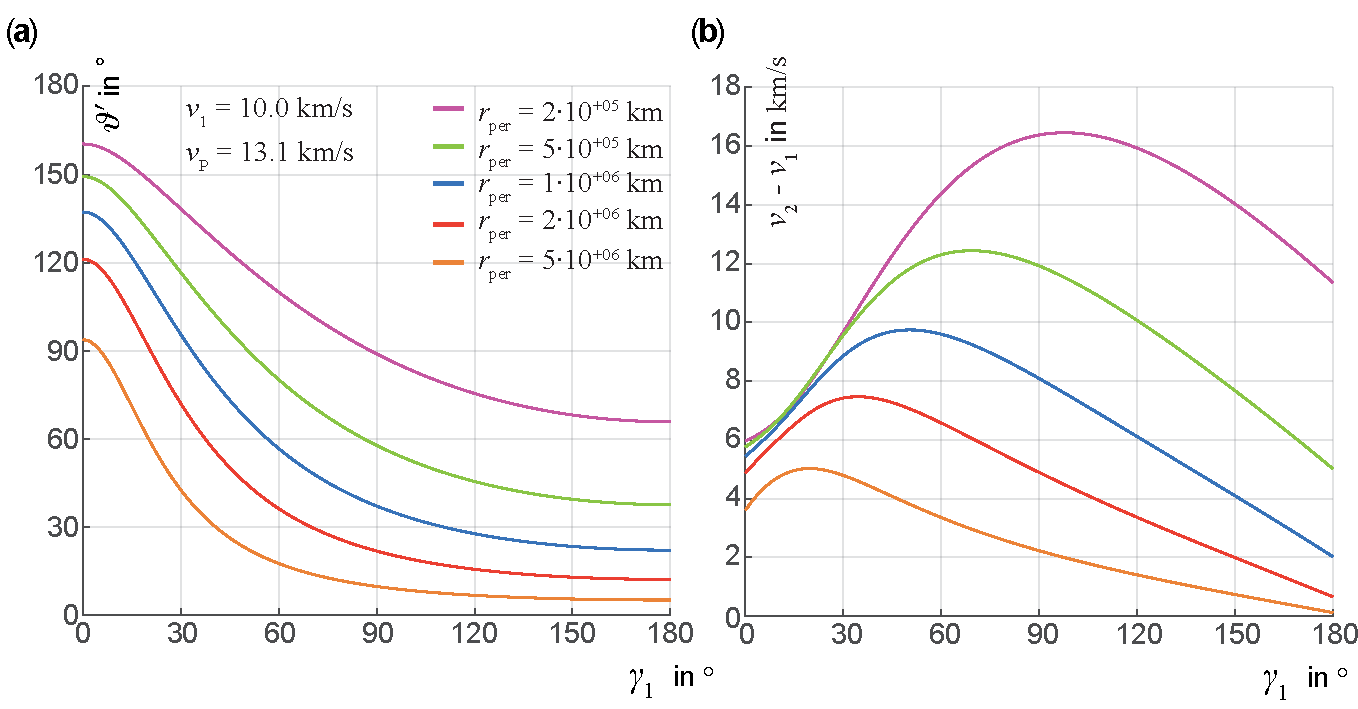
\includegraphics[width=\textwidth]{SwingByJupiter.pdf} 
	\caption[Swing-By-Man�ver am Jupiter.]{Swing-By-Man�ver am Jupiter.  \fa Streuwinkel $\vartheta'$  \fb Geschwindigkeitsgewinn $\vec{v}_2 - \vec{v}_1$ f�r verschiedene periplanetare Abst�nde $r_\text{per}$ als Funktion des Winkels $\gamma_1$.}
	\label{abb:adyn_swingby02}
\end{figure}

\begin{figure}[H]
	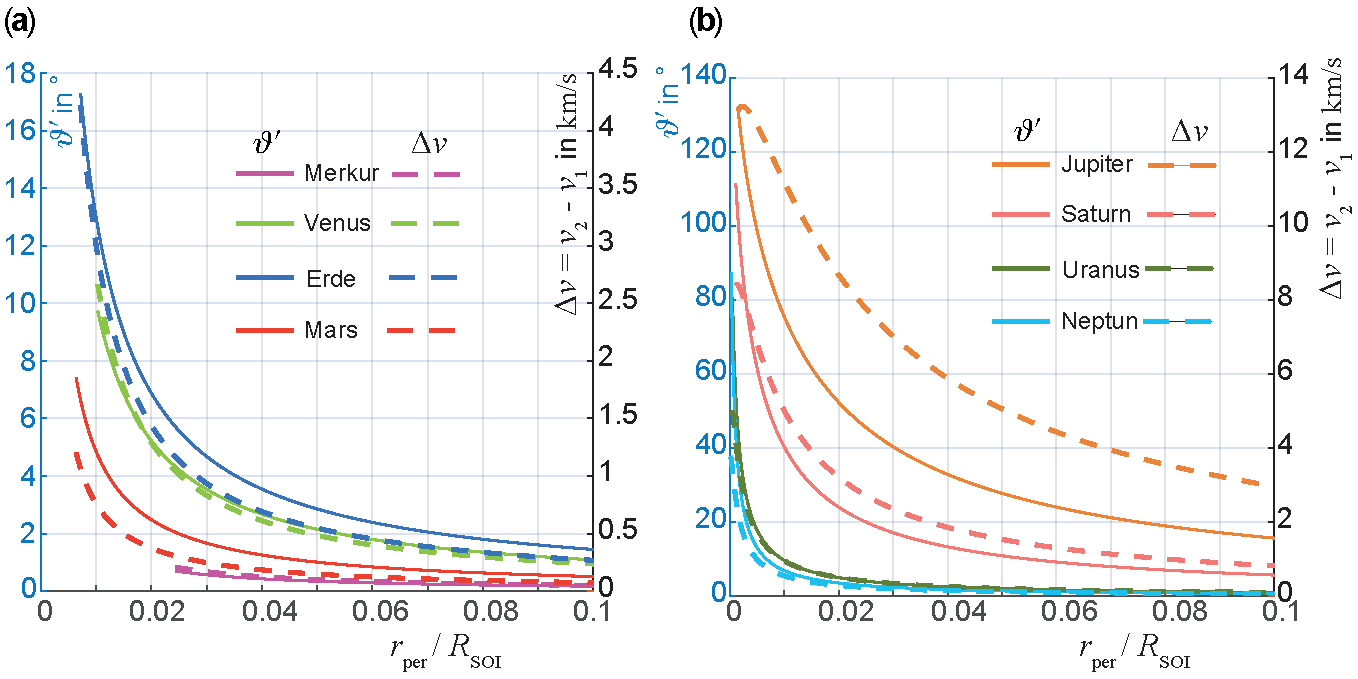
\includegraphics[width=\textwidth]{SwingByPlaneten.pdf} 
	\caption[Swing-By-Man�ver Ergebnisse bei den Planeten unseres Sonnensystems.]{Swing-By-Man�ver Ergebnisse bei den Planeten unseres Sonnensystems  als Funktion des periplanetaren Abstands $r_\text{per}$ normiert auf den Radius der SOI $R_\text{SOI}$, \fa innere Planeten \fb �u�ere Planeten. F�r die inneren Planeten wurde ein Eingangswinkel $\gamma_1 = 20\degree$ gew�hlt, f�r die �u�eren Planeten $\gamma_1 = 60\degree$. In beiden F�llen wurde $v_1= \SI{12.7}{\km\per\second}$ gesetzt. Alle anderen Werte siehe Tabelle \ref{tab:adyn_results_swingby}.}
	\label{abb:adyn_swingby02a}
\end{figure}

Da beim Swing-By $m_\text{P}$ (\bzw $\mu_\text{P}$) und $v_\text{P}$ festliegen, bleiben als freie Parameter nur $r_\text{per}$ und $\beta_1'$ (\bzw $\gamma_1$) �brig. Den Parameter $r_\text{per}$ k�nnen wir aus der Hyperbelgleichung berechnen:
\begin{align}
    r_\text{per} = a\lk 1- e\rk = \frac{\mu_\text{P}}{v_\infty{}^2}\,\lk e-1\rk \,, \label{eq:adyn_swingby16}
\end{align}
mit $e = 1/\cos\varphi'$. Der maximale Energie�bertrag erfolgt, wenn $\beta_2{}'=0$ ist, \dh die Vektoren $\vec{v}_2{}'$ und $\vec{v}_\text{P}$ parallel sind. Dann ist $\varphi'=90\degree-\beta_1{}'/2$ und somit $\cos\varphi'= \sin(\beta_1{}'/2)$ und wir erhalten f�r den optimalen Minimalabstand zum Perizentrum, bei dem der Energie�bertrag maximal wird: 
\begin{align}
    r_\text{P, opt} = \frac{\mu_\text{P}}{v_\infty{}^2}\,\lek \frac{1}{\sin\lk\beta_1{}'/2\rk}-1\rek > R_\text{P} \,.\label{eq:adyn_swingby17}
\end{align}
Dieser Abstand muss logischerweise immer gr��er als der physische Planetenradius $R_\text{P}$ sein, kann also durch geschickte Wahl von $v_1$ und $\gamma_1$ (und damit $v_1{}'$ und $\beta_1{}'$) entsprechend gew�hlt werden.\\
In \figref{adyn_swingby02a} haben wir $\Delta v = v_2-v_1$  und $\vartheta' = \Delta \gamma = \gamma_2 -\gamma_1$ als Funktion des Parameters $r_\text{per}$ �ber $\gamma_1$ dargestellt. \figref{adyn_swingby02} zeigt die gleichen Gr��en f�r die verschiedenen Planeten unseres Sonnensystems f�r einen vorgegebenen Wert von $v_1$ und $\gamma_1$ als Funktion des auf den Radius der SOI $R_\text{SOI}$ normierten Perizentrumsabstands $r_\text{per}$. Dabei haben wir f�r die Planeten jeweils den Bereich von $r_\text{per} = R_\text{P} + 500\,\mathrm{km}$ (inklusive Sicherheitsabstand von der Oberfl�che!) bis zu $0.1\,R_\text{SOI}$, \dh 10\% des Radius der jeweiligen SOI ausgew�hlt. Man erkennt, dass es signifikante Energie�bertr�ge vor allem bei den massereichen Planeten Jupiter und Saturn gibt, aber auch durch m�gliche "`nahe"' Vorbeifl�ge bei Venus und Erde (Tabelle \ref{tab:adyn_results_swingby}).\\ 

\begin{table}%tab 
\caption{Swing-By-Man�ver Daten f�r die Planeten unseres Sonnensystems.}
\smallskip
\begin{tabular}{L{0.8cm}R{1.35cm}R{1.65cm}R{1.25cm}R{1.25cm}R{1.25cm}R{1.25cm}R{1.65cm}R{1.25cm}}
\svhline\noalign{\smallskip}
Planet				& $v_\text{P}$                     & $m_\text{P}$     & $a_\text{P}$     & $R_\text{SOI}$  & $R_\text{P}$ & $v_{1,\text{max}{}'}$        & $\Delta H_\text{max}$& $\vartheta_\text{max}{}'$\\ 
\noalign{\smallskip}\noalign{\smallskip}              
& $\SI{}{\kilo\metre\per\second}$  & $\SI{}{\kg}$     & $10^6\,\SI{}{\km}$ & $10^6\,\SI{}{\km}$& $\SI{}{\km}$ & $\SI{}{\km\per\second}$   & $\SI{}{\joule\per\kg}$  &$\degree$\\ 
\noalign{\smallskip}\noalign{\smallskip}              
\noalign{\smallskip}\svhline\noalign{\smallskip} 
Merkur				& 47.9          & $\SI{3.28e23}{}$ &  57.9        & 0.11          & 2439         & 2.99                 & $\SI{1.43e8}{}$ & 6.1\\
Venus 				& 35.0          & $\SI{4.87e24}{}$ & 108.2        & 0.62          & 6051         & 7.33                 & $\SI{2.57e8}{}$ & 28.9\\
Erde 	  			& 29.8          & $\SI{5.97e24}{}$ & 149.6        & 0.93          & 6378         & 7.90                 & $\SI{2.35e8}{}$ & 32.4\\
Mars   				& 24.1          & $\SI{6.42e23}{}$ & 228.0        & 0.58          & 3394         & 3.55                 & $\SI{0.86e8}{}$ & 8.3\\
Jupiter 			& 13.1          & $\SI{1.90e27}{}$ & 778.4        &48.20          &71400         &42.1                  & $\SI{5.50e8}{}$ & 132.9\\
Saturn  			&  9.6          & $\SI{5.69e26}{}$ & 1425.5       &54.8           &60000         &25.2                  & $\SI{2.43e8}{}$ & 105.6\\
Uranus 				&  6.8          & $\SI{8.68e25}{}$ & 2870.4       &51.7           &26650         &15.0                  & $\SI{1.02e8}{}$ & 71.4\\
Neptun 				&  5.4          & $\SI{1.03e26}{}$ & 4501.1       &86.7           &24780         &16.7                  & $\SI{0.91e8}{}$ & 78.2\\
\svhline\noalign{\smallskip}
\end{tabular} \\
\label{tab:adyn_results_swingby}
\end{table}%tab 

Wie erw�hnt wird das Gravity-Assist-Man�ver bei vielen interplanetaren Raumfl�gen angewendet. 
Dabei benutzt man f�r die Missionsplanung die sogenannte \textit{Patched-Conic-} N�herung\index{Patched-Conic-N�herung}. Bei dieser N�herung wird die Trajektorie der Raumsonde in verschiedene Abschnitte unterteilt, indem jedem Himmelsk�rper (Sonne, Mond, Planeten) seine eigene Einflusssph�re (SOI) zugeordnet wird. Wenn die Sonde innerhalb der SOI des jeweiligen Himmelsk�rpers ist, wird nur dessen Gravitationskraft ber�cksichtigt, au�erhalb bei interplanetaren Fl�gen dann \ia nur die der Sonne. Dieses Vorgehen reduziert das $N$-K�rper-Problem auf ein Zweik�rperproblem, f�r das wir die bekannten parabolischen, elliptischen \bzw hyperbolischen L�sungen kennen.\footnote{Man �berlege sich, unter welchen Bedingungen die Methode nicht zum Erfolg f�hrt. Hinweis: Lagrange-Punkte (Band I, Kapitel 1.2.3.6.} 
Als Beispiel sei ein Erde-Mars-Transfer betrachtet (\vgl \probref{adyn_manoevers5}). Hier folgt die Raumsonde zun�chst einer hyperbolischen Bahn, um den Anziehungsbereich der Erde zu verlassen, dann folgt sie \ia einer Kepler-Ellipse um die Sonne, um schlie�lich in die Einflusssph�re des Mars zu treten. Durch das Zusammenf�gen der einzelnen Kegelschnittbahnen erh�lt man in guter N�herung die tats�chliche Bahn, daher auch der Name der N�herung (Englisch \textit{ to patch }- zusammenf�gen).\\
Selbstverst�ndlich kann man bei den Missionsplanungen zu �u�eren Planeten mit dieser Methode Gravity-Assist-Man�ver einbauen. In der Literatur (\ua \cite{Minovitch2010, Walter2018, Messerschmid2017}) finden sich dazu zahlreiche Beispiele. Wir wollen die zum Zeitpunkt des Verfassens dieses Buches im Jahre 2023 gestartete ESA-Mission JUICE (\textit{\underline{Ju}piter \underline{I}cy \underline{M}oon \underline{E}xploration}) etwas genauer betrachten und beziehen uns dabei auf \cite{Althaus2023}.

\begin{figure}[H]
	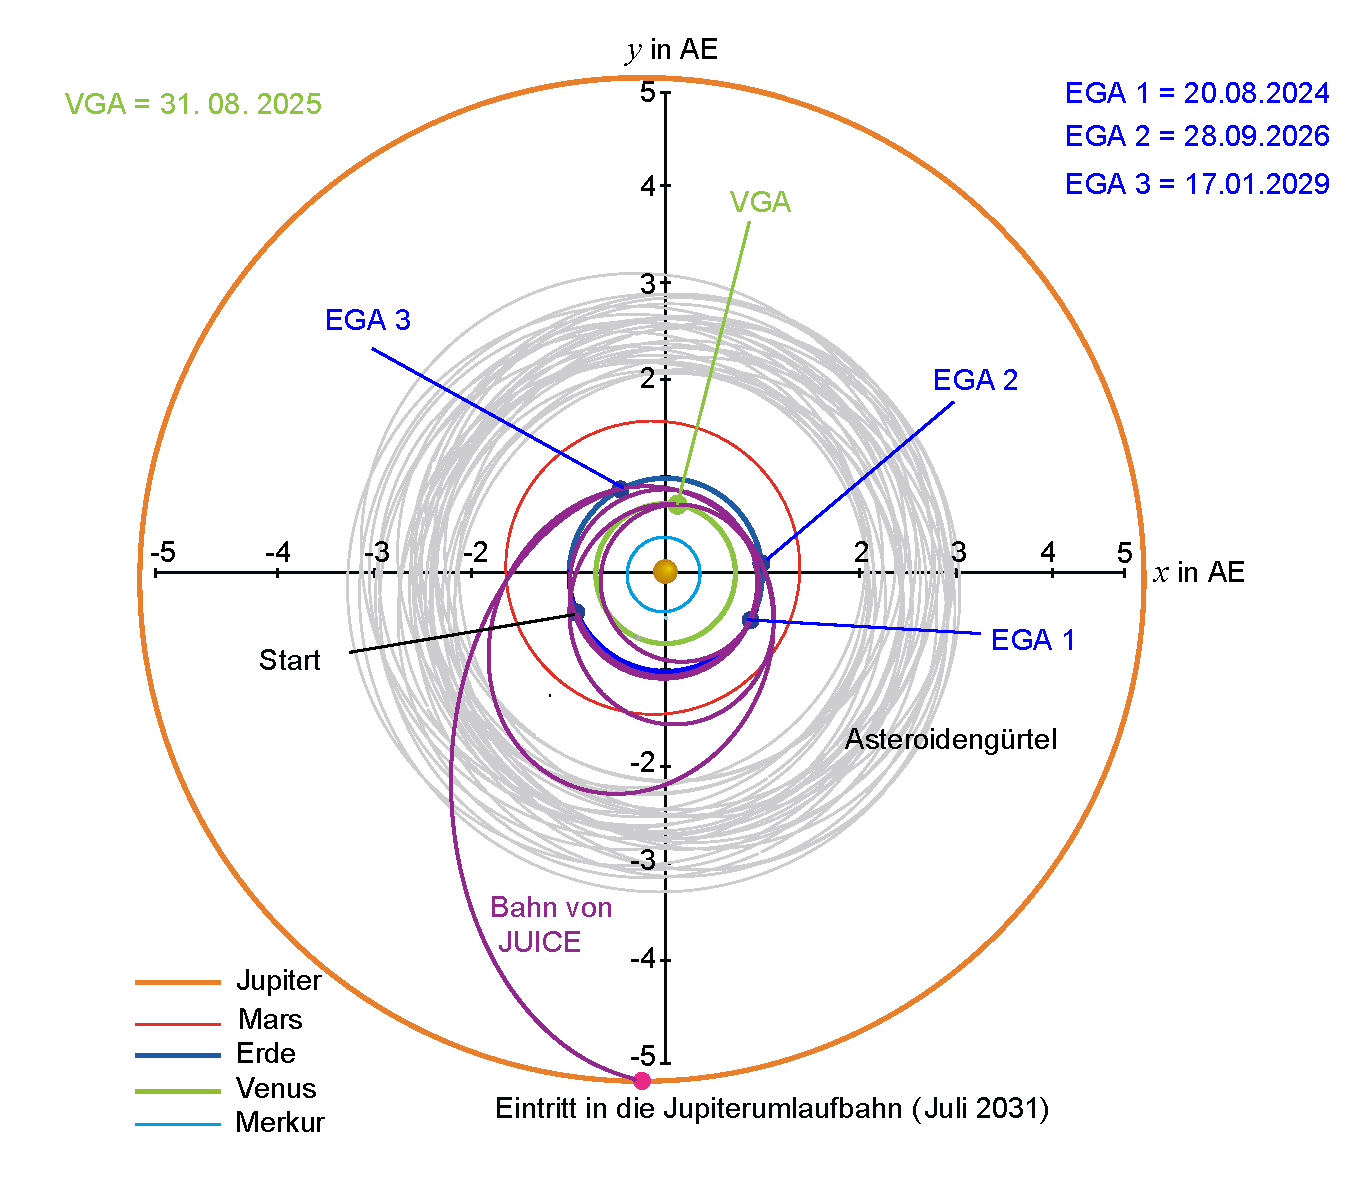
\includegraphics[width=\textwidth]{MissionJUICE.pdf} 
	\caption[Interplanetare Flugplanung der ESA-Mission JUICE.]{Interplanetare Flugplanung der ESA-Mission JUICE. Nach \cite{Althaus2023}.}
	\label{abb:adyn_PSP01}
\end{figure}

Die beeindruckende Reise dieser Raumsonde zu den Jupiter-Monden mit dem geplanten Eintritt in die Jupiterumlaufbahn im Jahr 2031 erfordert insgesamt vier Planeten-Vorbeifl�ge (\gls{GA}), dreimal an der Erde (EGA, \gls{EGA}) und einmal an der Venus (VGA, \gls{VGA}). Das erste EGA am 20.08.2024 f�hrte zu einer Abbremsung und damit zu einer engen Bahn um die Venus, von wo aus sie dann wieder beschleunigt wird und beim geplanten VGA am 31.08.2025 ein $\Delta v = \SI{3.8}{\km\per\second}$ erhalten wird ($r_\text{min} = \SI{5100}{\km} + R_\text{v}$). Der erneute Erdvorbeiflug am 28.09.2026 wird die Geschwindigkeit nochmals um $\Delta v = \SI{3.5}{\km\per\second}$ ($r_\text{min}= \SI{8600}{\km} + R_\text{E}$) erh�hen.\footnote{In \probref{adyn_PSP01} vergleichen wir die in den Vorbeifl�gen an Erde und Venus erreichten Geschwindigkeitszuw�chse von JUICE mit den maximal erreichbaren $\Delta v$ bei Venus und Erde (Tabelle \ref{tab:adyn_results_swingby}) und den Rechnungen in \probref{adyn_swingby01}.} 
%Die Sonde hat nun ausreichend Energie, um auf einer weiten elliptischen Bahn um die Sonne den Rand des Asteroideng�rtels zu erreichen, bevor sie 
Beim letzten EGA am 17.01.2029 wird sie noch ein $\Delta v = \SI{3.5}{\km\per\second}$ ($r_\text{min} = \SI{4600}{\,\km} + R_\text{E}$) bekommen, das sie endlich auf eine elliptische Bahn zum Jupiter (\figref{adyn_PSP01}) bringt. 

\subsection{Interplanetarer Raumflug zur Sonne}\label{kap:adyn_interplanetary_flights}

Wir hatten bereits in \figref{adyn_swingby00} gesehen, dass der Geschwindigkeitsgewinn $\Delta v$ bei einem Swing-By-Man�ver sowohl positiv als auch negativ sein kann. Wir wollen nun den Fall betrachten, bei dem man ein negatives $\Delta v$ braucht, um \zb eine Sonde so abzubremsen, dass sie auf eine sehr enge Umlaufbahn um die Sonne gelangen kann. Ein solche Mission ist die NASA-\textit{Parker}\footnote{Eugene Newman Parker (1927--2022) war ein US-amerikanischer Astrophysiker, der vor allem den Sonnenwind, die Magnetfelder von Erde und Sonne und deren komplexe Wechselwirkungen untersuchte. Er pr�gte auch als erster den Begriff \gls{Sonnenwind}\index{Sonnenwind} (\textit{solar wind}).}\indexp{Parker, Eugene Newman} \textit{Solar Probe}-Mission (PSP), die am 12.08.2018 gestartet wurde und zum Ziel hat, einen Minimalabstand zur Sonne von $r_\text{S}= \SI{0.05}{AE}$ zu erreichen. Was ist dabei eigentlich die Schwierigkeit? Man k�nnte meinen, dass eine Sonde einmal von der Erde in Richtung Sonne auf den Weg gebracht, von dieser so angezogen wird, dass die Sonde fr�her oder sp�ter in den Einfangbereich der Sonne gelangt und dann dort quasi von dieser in sich hineingezogen wird. Dem widersprechen aber die Gesetze der Himmelsmechanik, insbesondere die Drehimpuls- und Energieerhaltung. 
Um wirklich eine Sonde direkt zur Sonne zu senden, m�sste man ja durch Raketenenergie den Drehimpuls auf ann�hernd Null bringen, was bedeutet, dass man beim Start auf einer Erdbahn ein Antriebsbudget von etwa $\Delta v = - v_\text{E} = - \sqrt{2\mu_\text{S}/1\au} = -\SI{29.8}{\kilo\metre\per\second}$ haben muss. Die Sonne ist damit der am "`schwierigsten"' zu erreichende Platz in unserem Sonnensystem. 
Wir wollen den Antriebsbedarf etwas genauer absch�tzen, den man br�uchte, wenn man eine sonnennahe Bahn mit Minimalabstand $r_\text{min}$ durch einen Flug direkt aus einer Erdumlaufbahn erreichen wollte. Wir nehmen der Einfachheit halber einen Hohmann-Transfer mit $a_\text{H} = \frac{1}{2}\,\lk 1 \au + r_\text{min}\rk$ und $v_1 = v_\text{E} = \SI{29.8}{\km\per\second}$ an. Dann ergibt sich mit dem vis-viva-Satz\index{vis-viva-Satz} ein Geschwindigkeitsbedarf von 
\begin{align}
    \Delta v &\approx v_\text{P} -v_\text{E} = \sqrt{\mu_\text{S}\,\lk \frac{2}{0.05\au} - \frac{1}{a_\text{H}}\rk} - v_\text{E}
		= \sqrt{\frac{\mu_\text{S}}{1\au}}\,\sqrt{\lk \frac{2}{0.05\au} - \frac{2}{1.05\au}\rk} - v_\text{E} \nonumber  \\
		&= v_\text{E}\,\lk \sqrt{2\,\lk 1-\frac{1}{1.05}\rk} -1\rk \approx -\SI{20.6}{\km\per\second}\,.\label{eq:adyn_abschaetzung}
\end{align}
Mit der Ariane 5 schafft man es, eine Sonde mit einer Masse von $\SI{6}{\tonne}$ mit einer Geschwindigkeit von \ca $\SI{12.7}{\km\per\second}$ auf die Reise zu schicken (gemessen im \KOS\ der Erde, also vergleichbar mit dem $\Delta v$ aus \eqref{eq:adyn_abschaetzung}). Wir sehen also, dass es beim Stand der heutigen Raketentechnik nicht m�glich w�re, eine Sonde direkt zur Sonne zu schicken, die einen Minimalabstand von $0.05\,\au$ erreicht.\footnote{Zum Vergleich: Die gro�e Halbachse der Merkurbahn betr�gt $\SI{0.3871}{AE}$, also das etwa 8-fache.}
Wir wollen nun die Planung der PSP-Mission genauer betrachten. Die PSP soll die �u�ersten Atmosph�renschichten der Sonne und deren \gls{Korona}\index{Korona!der Sonne} erforschen und am 24.12.2024 den sonnenn�chsten Punkt der gesamten Mission mit $a_\text{P}= \SI{0.046}{}\,\au = \SI{6.8e6}{\kilo\metre}$ (Perihel ihres solaren Orbits) erreichen. Das ist nur das 18-fache des Erde-Mond-Abstands. N�her an die Sonne ist bisher noch keine Sonde gekommen. Die PSP nutzt bei ihrer Ann�herung an die Sonne verschiedene Gravity-Assists aus, um ihre Bahnenergie zu reduzieren. Wir wollen uns das Prinzip etwas genauer anschauen und treffen als Vereinfachung die Annahme, dass alle Bewegungen in der Ekliptik erfolgen.\\
Wenn eine Sonde von der Erde mit einem $\Delta \vec{v}_\text{R}$ gestartet wird, dann folgt diese einem elliptischen Orbit, der die SOI der Erde (oder auch der Venus) zu einem bestimmten Zeitpunkt wieder "`kreuzen"' wird, siehe \figref{adyn_swingby04}. An diesem Kreuzungspunkt $\mathrm{P}_1$ soll nun ein Gravity-Assist-Man�ver stattfinden.\footnote{Es gibt ja einen weiteren Kreuzungspunkt $\mathrm{P}_1'$, an dem ein Man�ver stattfinden kann. Zur Unterscheidung bezeichnen wir das Man�ver bei $\mathrm{P}_1$ als Planeten-ann�hernd und bei $\mathrm{P}_1'$ als Planeten-entfernend. Im weiteren wollen wir uns auf das erstere beschr�nken.} 

\begin{figure}[H]
	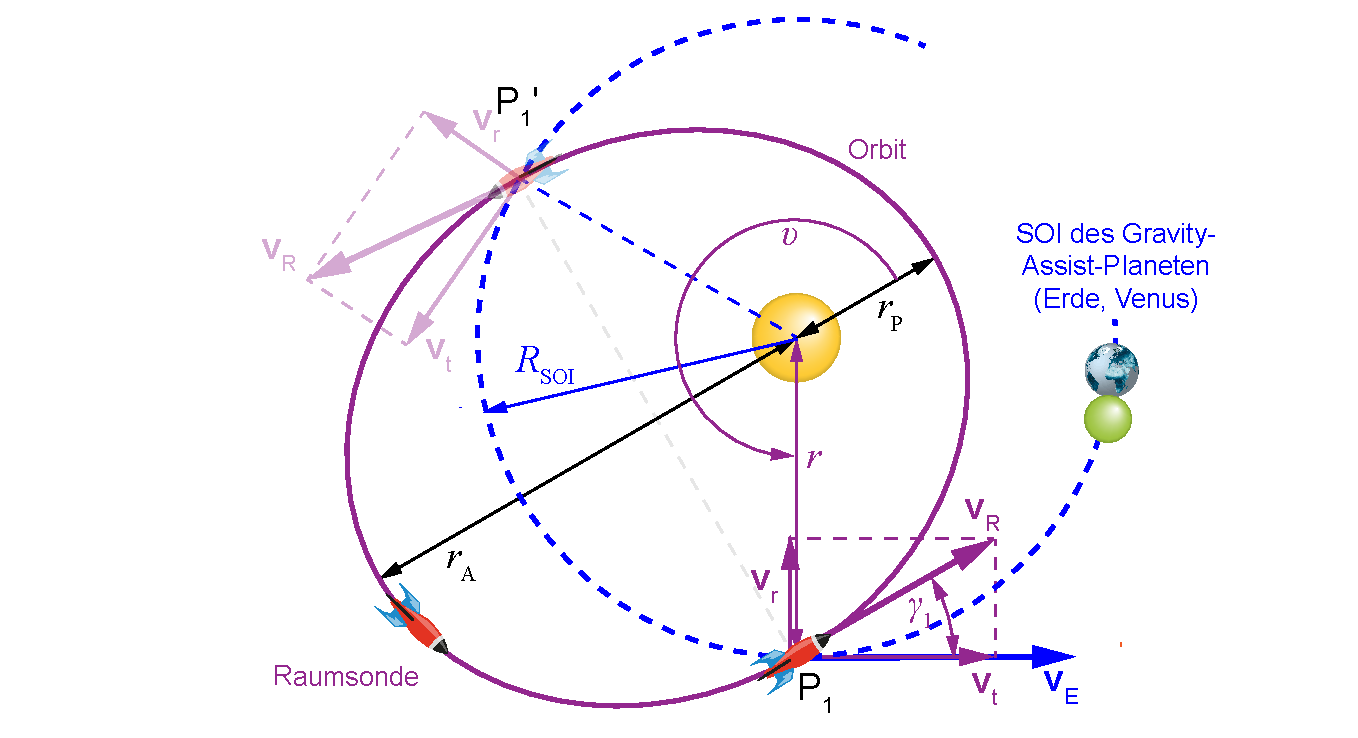
\includegraphics[width=\textwidth]{OrbitCrossing.pdf} 
	\caption[Gravity-Assist-Man�ver - Orbital Crossing.]{Gravity-Assist-Man�ver - Eine elliptische Bahn einer Sonde (lila) kreuzt die Einflusssph�re eines Planeten, hier der Erde (blau gezeichnet). Die Momentangeschwindigkeit der Sonde und auch die radiale und tangentiale Komponente sind als lila Vektoren dargestellt.}
	\label{abb:adyn_swingby04}
\end{figure}

Zur Berechnung brauchen wir den Vektor der Geschwindigkeit der Sonde an diesem Punkt~$\mathrm{P}_1$ im heliozentrischen Koordinatensystem. Dieser Vektor ist eine Funktion der Parameter der momentanen Bahn der Sonde und wir k�nnen ihn in einen radialen und einen zur SOI tangentialen Anteil zerlegen:
\begin{align}
	  \vec{v}_1 =\vec{v}_\text{R} = v_\text{r}\,\vec{e}_\text{r} + v_\text{t}\,\vec{e}_\text{t}\,.\label{eq:adyn_PSP01}
\end{align}
Dies hat den Vorteil, dass am Punkt $\mathrm{P}_1$ die Tangentialkomponente parallel zum Vektor der Planetengeschwindigkeit ist. Zur Vereinfachung nehmen wir an, dass die Sonde am Punkt~$\mathrm{P}_1$ zwar in die Einflusssph�re des Gravity-Assist-Planeten gelangt, aber immer noch einen Abstand zur Sonne von etwa dem Bahnradius (1\,AE f�r die Erde \bzw 0.723\,AE f�r die Venus) haben soll.\\
Wir nutzen die Erhaltungss�tze und schreiben mit $\mu_\text{S} = G\,m_\text{S}$ und den Parametern $a,\,e$ der Bahnellipse: 
\begin{align}
\begin{split}
	  \text{Drehimpulserhaltung, vgl. \eqref{eq:hm_drehimpuls_von_ae}} ~~~~L^2 &= r^2\, v_\text{t}{}^2 = \mu_\text{S}\,a\,\lk 1-e^2 \rk \,, \\
		\text{Energieerhaltung, vgl. \eqref{eq:hm_bewgl1}}~~~~H &= \frac{1}{2} \left| \vec{v}_\text{R} \right|^2 - \frac{\mu_\text{S}}{r} = - \frac{\mu_\text{S}}{2\,a}\,.
\end{split}  \label{eq:adyn_PSP02}
\end{align}
Aus der Ellipsengleichung \eqref{eq:hm_bahnglg}
\begin{align}
r(\upsilon) = \frac{a(1-e^2)}{1+e\,\cos\lk\upsilon-\upsilon_\text{P}\rk} \label{eq:adyn_PSP03}
\end{align}
mit $a = \lk r_\text{P} + r_\text{A} \rk /2$ und Perihel- \bzw Aphelabstand\index{Aphel}\index{Perihel} von $r_\text{P} = a\,(1-e)$ \bzw $r_\text{A} = a\,(1+e)$ erhalten wir f�r das Verh�ltnis von gro�er Halbachse $a$ der Sondenbahn und dem Radius der SOI, den wir vereinfacht schreiben als $R_0 = R_\text{SOI} = 1\,\au$ (\bzw $R_0 = 0.723\,\au$ f�r die Venus):
\begin{align}
	\frac{a}{R_0} = \frac{1}{2-\left|\vec{v}_\text{R} \right|^2 / v_0{}^2}\,, \label{eq:adyn_PSP04}
\end{align}
worin $v_0 = \sqrt{\mu_\text{S}/ R_0}$ ist. Aus \eqref{eq:adyn_PSP04} erhalten wir $\left|\vec{v}_\text{R} \right| = v_\text{R}$. Ferner folgt aus der Drehimpulserhaltung aus \eqref{eq:adyn_PSP02} f�r die Tangential- und Radialkomponente $v_\text{t}$ \bzw $v_\text{r}$
\begin{subequations}
\begin{align}
	v_\text{t} &= v_0\, \sqrt{\frac{a}{R_0}\,\lk 1-e^2 \rk} \,, \label{eq:adyn_PSP05a} \\
	v_\text{r} &= \sqrt{\left|\vec{v}_\text{R} \right|^2 - v_\text{t}{}^2} \,. \label{eq:adyn_PSP05b}
\end{align} 
\end{subequations} \label{eq:adyn_PSP05}

Damit k�nnen wir nun die f�r die Berechnung des Streuwinkels aus \eqref{eq:adyn_Streuung13b} noch fehlende Gr��e $v_\infty{}$ �ber \eqref{eq:adyn_swingby01a} berechnen: 
\begin{align}
	v_\infty{}  = \sqrt{v_\text{r}{}^2 - \lk v_\text{t} - v_0 \rk^2} \,. \label{eq:adyn_PSP06}
\end{align} 
Wir setzen nun f�r die initiale Bahn (Index a) der PSP die Werte $r_\text{P} = 0.207\,\au,\,~r_\text{A} = 1.013\,\au$ ein und erhalten: 
\begin{align*}
  v_\text{t} &= \SI{24.1}{\km\per\second}\,,~~~v_\text{r} = \SI{20.4}{\km\per\second}\,,~~~v_0 = \SI{35.02}{\km\per\second}\,~~
	\rightarrow v_\infty{}  = \SI{23.4}{\km\per\second}\,.
\end{align*}
F�r die Venus erhalten wir mit $\mu_\text{V} = G\,m_\text{V}$ f�r $\tilde{v}_\text{F}$ aus \eqref{eq:adyn_swingby09c}:
\begin{align}
    \tilde{v}_\text{F} &= \sqrt{\frac{2 \mu_\text{V}}{R_\text{V} + \SI{500}{km}}} = \SI{9.95}{\km\per\second}\,, \label{eq:adyn_PSP07} 
\end{align}
woraus sich bei einem Sicherheitsabstand des Swing-By-Man�vers von 500 km von der Venusoberfl�che ein maximaler Streuwinkel von $\vartheta'_\text{a} = 9.73\degree$ ergibt. 

\begin{table} [ht] %tab 
\caption{Die einzelnen Orbits der NASA Mission Parker Solar Probe I um die Sonne.}
\smallskip
\begin{tabular}{C{0.8cm}R{1.5cm}R{1.5cm}R{1.5cm}C{1.5cm}R{1.75cm}R{1.75cm}}
\svhline\noalign{\smallskip}
Orbit &  $r_\text{P} \, (\au)$  & $r_\text{A} \, (\au)$ & $\beta_1'\, (\degree)$ &   $ e $    &  $ T_\text{Bahn}$ \, (Tage) & $v_\text{P}\,(\SI{}{\km\per\second})$\\
\noalign{\smallskip}\svhline\noalign{\smallskip} 
\noalign{\smallskip}\noalign{\smallskip}              
  a    &   0.207     &   1.013    &   61.94     &  0.661   &    174.0     &   84.35 \\
  b    &   0.166     &   0.938    &   55.58     &  0.699   &    149.8     &   95.29 \\
  c    &   0.130     &   0.874    &   48.43     &  0.741   &    129.9     &  108.99 \\
  d    &   0.095     &   0.817    &   39.42     &  0.792   &    112.5     &  129.34 \\
  e    &   0.074     &   0.783    &   31.99     &  0.827   &    102.5     &  147.99 \\
  f    &   0.062     &   0.761    &   25.77     &  0.849   &     96.4     &  162.65 \\
  g    &   0.053     &   0.745    &   19.74     &  0.867   &     92.1     &  176.77 \\
  h    &   0.046     &   0.731    &   11.99     &  0.882   &     88.5     &  190.47 \\
\svhline\noalign{\smallskip}
\end{tabular} \\
\label{tab:adyn_PSP01}
\end{table}%tab 

Dieser Streuwinkel ist deutlich kleiner als der notwendige Streuwinkel von $\Delta \vartheta' = \beta_{1,\text{a}}{}' - \beta_{1,\text{h}}{}' \approx 50\degree$, den man br�uchte, wenn man durch ein Swing-By-Man�ver direkt von der Anfangsbahn mit $r_\text{P,a} = 0.207\,\au,\,~r_\text{A,a} = 1.013\,\au$ auf die vorgesehene finale Bahn mit $r_\text{P,h} = 0.046\,\au,\,~r_\text{A,h} = 0.731\,\au$ gelangen m�chte. Dazu br�uchte man (siehe Tabellen \ref{tab:adyn_PSP01} und \ref{tab:adyn_PSP02}) also mindestens 6 Gravity-Assist-Man�ver an der Venus. Die tats�chliche Mission nutzte insgesamt 7 solcher Swing-By-Man�ver, deren Abfolge mit den einzelnen Streuwinkeln, den kumulierten Streuwinkeln und den realisierten Perizentrumsabst�nden $R_\text{V,real}$ der jeweiligen Swing-By-Man�ver in Tab. \ref{tab:adyn_PSP02} und \figref{adyn_swingby05} dargestellt sind. Eine vertiefte Betrachtung zu der Missionsplanung der PSP, in der auch ein elegantes graphisches Tool zur Bestimmung der Bahnen, die sogenannte \textit{Velocity-Space-Map},  vorgestellt wird, findet sich in \cite{Longcope2020}.

\begin{table} [ht] %tab 
\caption{Die einzelnen Swing-By-Man�ver der NASA Mission Parker Solar Probe I an der Venus.}
\smallskip
\begin{tabular} {C{1.75cm}R{1.75cm}R{1.75cm}R{1.75cm}}
\svhline\noalign{\smallskip}
GA-Man�ver &  $\vartheta' \,(\degree)$  &  $\sum\vartheta'\, (\degree)$  & $R_\text{V,real}/R_\text{V}$\\
\noalign{\smallskip}\svhline\noalign{\smallskip} 
\noalign{\smallskip}\noalign{\smallskip}              
   1\,:\;(a $\,\rightarrow\,$ b)  &    6.501    &      6.501        &   1.67  \\
   2\,:\;(b $\,\rightarrow\,$ c)  &    7.157    &     13.658        &   1.49  \\
   3\,:\;(c $\,\rightarrow\,$ d)  &    9.113    &     22.771        &   1.15  \\
   4\,:\;(d $\,\rightarrow\,$ e)  &    7.389    &     30.160        &   1.43  \\
   5\,:\;(e $\,\rightarrow\,$ f)  &    6.229    &     36.389        &   1.70  \\
   6\,:\;(f $\,\rightarrow\,$ g)  &    5.948    &     42.337        &   1.79  \\
   7\,:\;(g $\,\rightarrow\,$ h)  &    7.628    &     49.965        &   1.37  \\
\svhline\noalign{\smallskip}
\end{tabular} \\
\label{tab:adyn_PSP02}
\end{table}%tab 

\begin{figure}[H]
	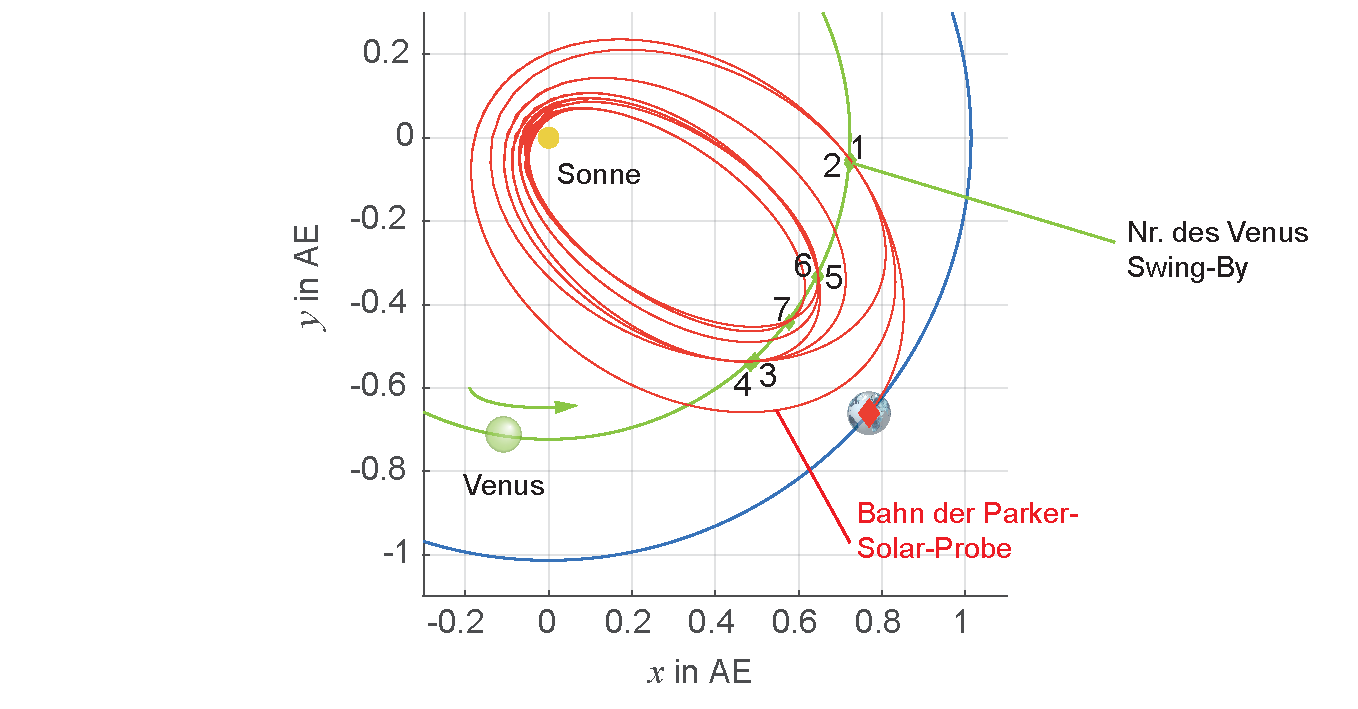
\includegraphics[width=\textwidth]{BahnParkerSolarProbe.pdf} 
	\caption[Die NASA Mission Parker Solar Probe.]{Die NASA Mission Parker Solar Probe. Dargestellt ist die Bahn der PSP vom Start bis zum 30.1.2024. Die Rauten geben die Punkte der Venus-Swing-By-Man�ver an. Die Daten der PSP-Bahn stammen vom JPL \cite{JPL2020}, k�nnen aber nat�rlich genau so wie die Planetenbahnen von Venus und Erde mit den Methoden aus dem \kap{hm_bahnen_hk_ss} aus der Himmelsmechanik berechnet werden. Sehr gut zu erkennen ist, wie mit jedem Swing-By-Man�ver die Sonde sukzessive auf eine engere Bahn um die Sonne gelangt. Siehe auch \probref{adyn_PSP01} und \mscr~ \mladynref{ParkerSolarProbe.m}.}
	\label{abb:adyn_swingby05}
\end{figure}















\section{Rendezvous im Weltall}\label{kap:adyn_planetflights}

\subsection{Dynamik und Kinematik eines Kopplungsman�vers }\label{kap:adyn_rendezvous}

Wir wollen uns jetzt das Rendezvous\index{Rendezvouz} (\bzw das Andocken) zwischen zwei Raumschiffen, \zb einem Raumtransporter (\emph{"`Verfolger"'}, englisch \textit{Interceptor, Chaser}, Index J) und einer Raumstation (\zb der ISS) in einer Umlaufbahn  (dem \textit{"`Ziel"'}, englisch \textit{Target}, Index T) anschauen und folgen hier der Darstellung in \cite{Carroll2019}.
Die mathematische Beschreibung des Rendezvous von zwei Raumschiffen im Weltall ist relativ komplex, was unter anderem auch daran liegt, dass die Bewegung der beiden Raumschiffe zueinander, wenn man sie aus einem mit einem der Raumschiffe verbundenen Koordinatensystem beschreibt, dann in einem rotierenden nicht inertialen Koordinatensystem beschrieben werden muss\footnote{Wir werden dabei gewisse �hnlichkeiten mit dem Fahren auf einer rotierenden Scheibe (\vgl �bung 1.21 in Band I) feststellen.}.\\
Wir bezeichnen das Inertialsystem mit Ursprung im Erdmittelpunkt mit $\vec{\Sigma}$ und das mitbewegte System, welches seinen Ursprung im Ziel (in der ISS) mit $\vec{\Sigma}'$. Die $z$-Achsen beider Systeme sind parallel und zeigen senkrecht aus der Bahnebene heraus (\figref{adyn_rendezvousKOS01}). Die Koordinaten des Verfolgers (des Raumtransporters) haben daher einen Strich, wenn sie vom Ziel aus gemessen werden, sie sind ohne Strich, wenn sie von der Erde aus gemessen werden.\\
F�r die Kopplung\footnote{Wir benutzen den Begriff Kopplung und Rendezvous hier synonym, obwohl im strengen Sinne der Astrodynamik mit Rendezvous die Begegnung zweier Raumschiffe durch entsprechende Bahnman�ver und mit Kopplung der gesamte mechanische Vorgang der Verbindung zweier Raumschiffe bezeichnet wird.} zweier Objekte im Weltall muss zum Zeitpunkt $t_\text{K}$ der Kopplung im Koordinatensystem der Erde $\vec{\Sigma}$ \bzw im System des Ziels $\vec{\Sigma}'$ gelten:
\begin{align}
\begin{split}
    \vec{\Sigma}: ~~~~ \vec{r}_\text{T}\lk t_\text{K}\rk &= \vec{r}_\text{J}\lk t_\text{K}\rk ~~ \text{und} ~~~  \dot{\vec{r}}_\text{T}\lk t_\text{K}\rk = \dot{\vec{r}}_\text{J}\lk t_\text{K}\rk \,, \\
    \vec{\Sigma}': ~~~\,~  \vec{r}'\lk t_\text{K}\rk &= 0 ~~ \text{und} ~~~ \dot{\vec{r}}'\lk t_\text{K}\rk = 0 \,. 
\end{split} \label{eq:adynrendez01}
\end{align}
Die Bedingungen f�r die Geschwindigkeit sichern eine \anf{weiche} Kopplung.\\
Wir bezeichnen die Position des Ziels (\figref{adyn_rendezvousKOS01}) im Inertialsystem mit:
\begin{align}
    \vec{R} = X\,\vec{e}_x + Y\,\vec{e}_y + 0\,\vec{e}_z = R_0\,\vec{e}_{y'} ~~~~ \text{mit} ~~~~ R_0 = \sqrt{X^2+Y^2}\,,\label{eq:adyn_rendez01}
\end{align}
entsprechend die des Verfolgers mit
\begin{align}
    \vec{r} = x\,\vec{e}_x + y\,\vec{e}_y + z\,\vec{e}_z\label{eq:adyn_rendez02}\,,
\end{align}
\bzw im mitbewegten \KOS\ mit
\begin{align}
    \vec{r}' = x'\,\vec{e}_{x'} + y'\,\vec{e}_{y'} + z'\,\vec{e}_{z'}\label{eq:adyn_rendez03}\,.
\end{align}
%Um ein Rendezvous im Weltall durchzuf�hren, ist die Beschreibung der Bewegung als Relativbewegung von Ziel und Verfolger sinnvoll, und zwar am einfachsten vom Ziel aus betrachtet. 
Es gelten dann folgende Bewegungsgleichungen f�r die Koordinaten des Verfolgers im nichtinertialen \KOS\ des Ziels:
\begin{align}
\begin{split}
    \vec{r}' &= \vec{r} - \vec{R}\,,\\
    \dot{\vec{r}}' &= \dot{\vec{r}} - \dot{\vec{R}} - \vec{\omega}'\times\vec{r}'\,,\\
    \ddot{\vec{r}}' &= \ddot{\vec{r}} - \ddot{\vec{R}} - \vec{\omega}'\times\lk\vec{\omega}'\times\vec{r}'\rk-2\vec{\omega}'\times\dot{\vec{r}}'-\dot{\vec{\omega}}' \times\vec{r}'\,.
\end{split} \label{eq:adyn_rendez04}
\end{align} 
Wir wissen aus der Himmelsmechanik, dass f�r Kepler-Bahnen Drehimpulserhaltung und $\dot{\vec{\omega}} = 0$ gilt, so dass wir mit dem Kreisbahnradius $R_0$ des Ziels  schreiben k�nnen:
\begin{align}
    \vec{\omega}' = -\omega_0\,\vecpeZ = -\omega_0\,\veceZ ~~~~ \text{mit} ~~~~ \omega_0 = \sqrt{\frac{G\,m_\text{E}}{R_0{}^3}}\,.  \label{eq:adyn_rendez04a}
\end{align}
F�r den Term $-\vec{\omega}'\times\lk\vec{\omega}'\times\vec{r}'\rk$ finden wir durch einfache Rechnung:
\begin{align}
    -\vec{\omega}' \times\lk\vec{\omega}'\times\vec{r}'\rk = \omega_0{}^2\,\lk x'\, \vecpeX +  y'\, \vecpeY \rk = \omega_0{}^2\,\vec{r}' - \omega_0{}^2\, z'\, \vecpeZ
\end{align} \label{eq:adyn_rendez05}
und f�r $\ddot{\vec{R}}$ 
\begin{align}
    \ddot{\vec{R}} = -\omega_0{}^2\,\vec{R}= -\frac{G\,m_\text{E}}{R_0{}^3}\,\vec{R} \label{eq:adyn_rendez06}\,.
\end{align}

\begin{figure}[H]
	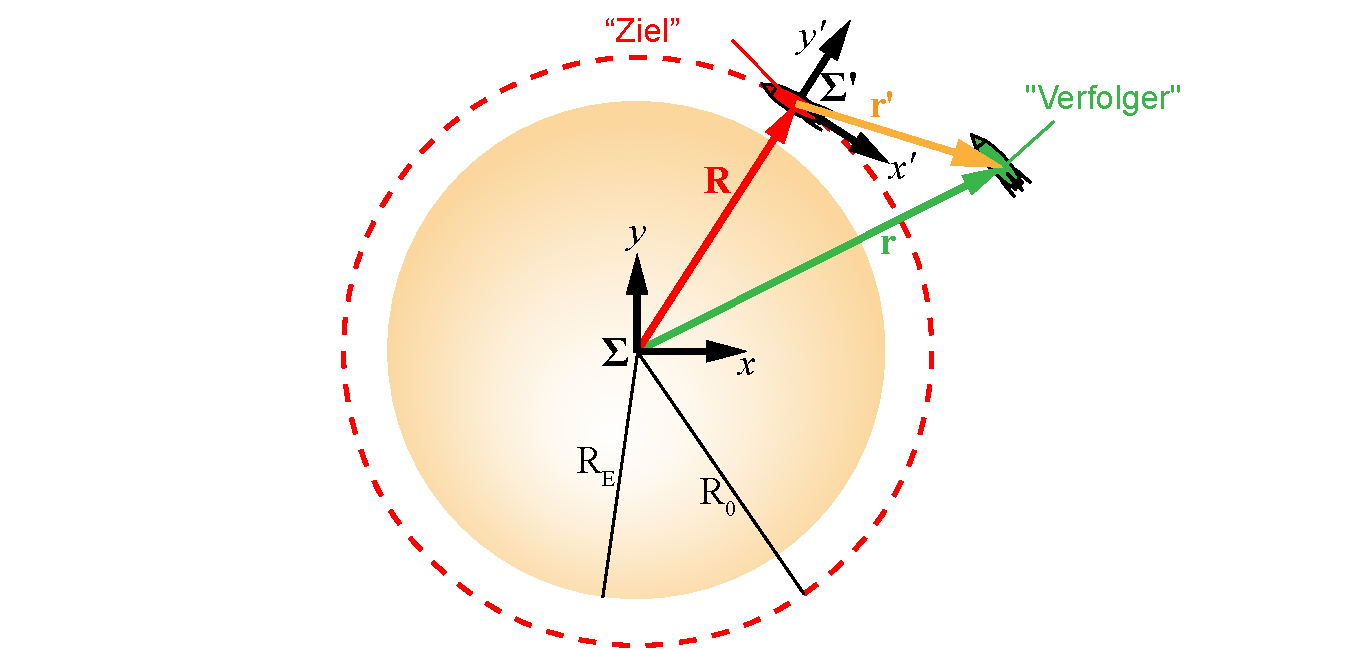
\includegraphics[width=\textwidth]{RendezvousKOS01.pdf} 
	\caption[Koordinatensysteme f�r Rendezvous in der Umlaufbahn.]{Koordinatensysteme f�r Rendezvous in der Umlaufbahn. Wir nehmen zun�chst eine Bewegung der beiden Raumschiffe in der $x$-$y$-Ebene an. Das Inertialsystem $\vec{\Sigma}$ ist in der Erde \bzw dem Mond zentriert, das Nicht-Inertialsystem $\vec{\Sigma}'$ auf dem Ziel-Raumschiff, welches sich mit konstanter Winkelgeschwindigkeit um die Erde \bzw den Mond bewegt. Die $z$-Achse zeigt aus der Papierebene heraus.}
	\label{abb:adyn_rendezvousKOS01}
\end{figure}

Unter Ber�cksichtigung der Gravitationskraft der Erde $\vec{F}_\text{G} =-G\,m_\text{E}\,m_\text{R}\,\vec{r}/ r{}^3 $ und anderer nichtgravitativer Kr�fte $\vec{F}$ (wie \zb Reibung, Schub) ergeben sich dann folgende Bewegungsgleichungen (in drei Dimensionen), wobei $m_\text{R}$ die Masse des Raumschiffs ist:
\begin{align}
\begin{split}
    \ddot{\vec{r}}' &= G\,m_\text{E}\lk\frac{1}{R_0{}^3}-\frac{1}{r^3}\rk\,\vec{r} - \omega_0{}^2\,z'\,\vec{e}_{z'} - 2\vec{\omega}\times\dot{\vec{r}}' + \frac{\vec{F}}{m_\text{R}} \\
    &= \omega_0{}^2 \,\lk 1-\frac{R_0{}^3}{r^3}\rk\,\vec{r} - \omega_0{}^2\,z'\,\vec{e}_{z'} -2\vec{\omega} \times\dot{\vec{r}}' + \frac{\vec{F}}{m_\text{R}} \; .
\end{split}\label{eq:adyn_rendez07}
\end{align}
F�r kleine Abst�nde $r'$ wollen wir diese Gleichung nach $x',\,y',\,z'$ entwickeln und schreiben deshalb den Term mit $1/r^3$ wie folgt:\footnote{Das haben wir ja bereits ausgiebig ge�bt, \zb im \kap{hm_gezeiten}.}
\begin{align}
\begin{split}
    \lk 1-\frac{R_0{}^3}{r^3}\rk\,\omega_0{}^2\,\vec{r} &= \lek 1-\frac{R_0{}^3}{\sqrt{\lk x'{}^2 + \lk R_0+y' \rk^2+z'{}^2\rk^3}}\rek \,\omega_0{}^2\,\lk \vec{r}' + \vec{R} \rk\\
    &= \lek 1-\frac{1}{\sqrt{\lk\lk \frac{x'}{R_0}\rk^2 +\lk 1+\frac{y'}{R_0}\rk^2 + \lk \frac{z'}{R_0}\rk^2\rk^3}}\rek\,\,\omega_0{}^2\,\lk \vec{r}' + R_0\,\vec{e}_{y'}\rk \,.
\end{split} \label{eq:adyn_rendez08}
\end{align}
Wir k�nnen nun $x'/R_0,\,y'/R_0\,,z'/R_0\,\ll\, 1$ annehmen, so dass der Term in der rechteckigen Klammer zu $ \lk 1-\lk 1+2\frac{y'}{R_0}\rk^{-3/2} \rk  = \lk 1-\lk 1-3\frac{y'}{R_0}\rk\rk$ wird und somit aus \eqref{eq:adyn_rendez08}:
\begin{align}
\begin{split}
    \lk 1-\frac{R_0{}^3}{r^3} \rk \, \omega_0{}^2\,\vec{r} 
		&\approx \omega_0{}^2 \lk 3\,\frac{y'}{R_0}\rk \lk x'\,\veceX + y'\,\veceY + z'\,\veceZ + R_0\,\vecpeY\rk \approx 3y' \, \omega_0{}^2 \, \vec{e}_{y'} \,.
\end{split} \label{eq:adyn_rendez09}
\end{align}
Analog l�sst sich zeigen, dass f�r das Kreuzprodukt in \eqref{eq:adyn_rendez07} gilt:
\begin{align}
    -2\vec{\omega}'\times\dot{\vec{r}}' = -2\,\omega_0\,\dot{y}'\,\vecpeX + 2\,\omega_0\,\dot{x}'\,\vecpeY \,. \label{eq:adyn_rendez10}
\end{align}
Damit ergibt sich aus \eqref{eq:adyn_rendez07}:
\begin{align}
    \ddot{\vec{r}}' = 3\,\omega_0{}^2\,y'\,\vec{e}_{y'}  - \omega_0{}^2\,z'\,\vec{e}_{z'}  + 2\,\omega_0\,\dot{x}'\,\vec{e}_{y'}  -2\,\omega_0\,\dot{y}'\,\vec{e}_{x'}  + \frac{\vec{F}}{m_\text{R}}\,. \label{eq:adyn_rendez11}
\end{align}
Man erkennt an \eqref{eq:adyn_rendez11} die verschiedenen Beitr�ge. Der erste Term ist eine Gezeitenkraft, die Terme mit $\dot{x}'$ \bzw $\dot{y}'$ sind Beitr�ge der Coriolis-Kraft. In Komponenten und Matrixform geschrieben wird aus \eqref{eq:adyn_rendez11}:
\begin{align}
    \begin{pmatrix}
        \ddot{x}'\\
        \ddot{y}'\\
        \ddot{z}'
    \end{pmatrix}
    = 2\omega_0
    \begin{pmatrix}
      -\dot{y}'\\
      \dot{x}'\\
      0
    \end{pmatrix}
    +\omega_0^2
    \begin{pmatrix}
        0\\
        3y'\\
        -z'
    \end{pmatrix}
    + \frac{1}{m_\text{R}}
    \begin{pmatrix}
        F_{x'}\\
        F_{y'}\\
        F_{z'}
    \end{pmatrix} \,.\label{eq:adyn_rendez22}
\end{align}
%\begin{align}
    %\begin{pmatrix}
        %\ddot{x}'\\
        %\ddot{y}'\\
        %\ddot{z}'
    %\end{pmatrix}
%=
    %\begin{pmatrix}
       %-2\,\omega_0\,\dot{y}'\\
        %2\,\omega_0\,\dot{x}' + 3\,\omega_0{}^2\,y' \\
        %-\omega_0{}^2\,z'
    %\end{pmatrix} \,+ \,
		%\begin{pmatrix}
       %F_{x'}/m_\text{R}\\
       %F_{y'}/m_\text{R}\\
       %F_{z'}/m_\text{R}
    %\end{pmatrix} \, . \label{eq:adyn_rendez12a}
%\end{align}
%\begin{subequations}
%\begin{align}
    %\ddot{x}' &= -2\,\omega_0\,\dot{y}' + \frac{F_{x'}}{m_\text{R}} \,,\\
    %\ddot{y}' &= 2\,\omega_0\,\dot{x}' + 3\,\omega_0{}^2\,y'+ \frac{F_{y'}}{m_\text{R}}\,,\\
    %\ddot{z}' &= -\omega_0{}^2\,z' + \frac{F_{z'}}{m_\text{R}}\,.
%\end{align}\label{eq:adyn_rendez12}
%\end{subequations}
Diese Gleichungen werden in der Literatur als \emph{Hill\footnote{George William Hill (1838--1914) war ein US-amerikanischer Astronom und Mathematiker, dessen Methoden zur Bahnberechnung von Himmelsk�rpern bis heute u.a. auch in der Raumfahrt verwendet werden.}-Gleichungen}\index{Hill-Gleichungen}\indexp{Hill, George William} bezeichnet. \\
Wir wollen diese nun unter der Annahme impulsiver Man�ver l�sen, so dass wir $F_{x'}$, $F_{y'}$, $F_{z'}$ alle gleich Null setzen k�nnen. Die Gleichung f�r $\ddot{z}'(t)$ ist vollkommen von den anderen Gleichungen entkoppelt und man erh�lt sofort f�r $z'\lk t\rk$ die L�sung 
\begin{align}
\begin{split}
    z'\lk t\rk &= z_0'\,\cos\lk \omega_0 t\rk + \frac{\dot{z}_0'}{\omega_0}\,\sin\lk \omega_0 t\rk, \\
    \dot{z}'\lk t\rk &= -z_0'\,\omega_0\,\sin\lk \omega_0 t\rk + \dot{z}_0'\,\cos\lk \omega_0 t\rk \,.
\end{split}  \label{eq:adyn_rendez13}
\end{align} 
Das bedeutet, dass das Raumschiff in $z'$-Richtung eine harmonische Bewegung ausf�hrt, deren Periode durch die Umlaufzeit $T_0 = 2\pi/\omega_0=2\pi\sqrt{R_0{}^3/(G m_\text{E})}$ des Ziels definiert ist. Das bedeutet aber auch, dass durch die entsprechende Wahl von $z_0'$ und $\dot{z}_0'$ diese Bewegung so kompensiert werden kann, dass das Rendezvous-Man�ver nur in der $x',y'$-Ebene stattfindet und dort betrachtet werden muss. In dieser Ebene gibt es nun ein interessantes Wechselspiel von Gezeiten- und Coriolis-Kraft. \\
Wir wollen die Hill-Gleichungen \eqref{eq:adyn_rendez22} weiter l�sen und nehmen die Anfangsbedingungen $x_0'$, $\dot{x}_0'$, $y_0'$ und $\dot{y}_0'$ als gegeben an. Die L�sung erfolgt �hnlich zu der, die in Kapitel 1.3.2 in Band I f�r die Bewegungsgleichungen eines Massepunktes im \KOS\ der rotierenden Erde gezeigt wurde. Wir erhalten anstelle der zwei Differentialgleichungen zweiter Ordnung nun vier Differentialgleichungen erster Ordnung:
\begin{subequations}
\begin{align}
    x'\lk t\rk = &\lk 6\,y_0' +4\,\frac{\dot{x}_0'}{\omega_0}\rk\,\sin\lk \omega_0 t\rk + \frac{2\dot{y}_0'}{\omega_0}\,\cos\lk \omega_0 t\rk + x_0' -2\,\frac{\dot{y}_0'}{\omega_0} - \lk 6\,\omega_0\,y_0' + 3\,\dot{x}_0'\rk\,t\,, \label{eq:adyn_rendez14a} \\
\dot{x}'\lk t\rk = &\lk 6\,\omega_0\,y_0' +4\,\dot{x}_0'\rk\,\cos\lk\omega_0 t\rk - 2\,\dot{y}_0'\,\sin\lk\omega_0t\rk - 6\,\omega_0\,y_0'-      3\,\dot{x}_0' \,, 
\label{eq:adyn_rendez14b} \\
y'\lk t\rk = &-\lk 3\,y_0' +2\,\frac{\dot{x}_0'}{\omega_0}\rk\,\cos\lk \omega_0 t\rk + \frac{\dot{y}_0'}{\omega_0}\,\sin\lk \omega_0 t\rk + 4\,y_0' + 2\,\frac{\dot{x}_0'}{\omega_0} \,, \label{eq:adyn_rendez14c} \\
\dot{y}'\lk t\rk = &\lk 3\,\omega_0\,y_0' +2\,\dot{x}_0'\rk\,\sin\lk\omega_0 t\rk + \dot{y}_0'\,\cos\lk\omega_0t\rk \,. \label{eq:adyn_rendez14d}
\end{align} 
\end{subequations}
Diese Gleichungen zusammen mit \eqref{eq:adyn_rendez13} hei�en \gls{CWG}\index{Clohessy-Wiltshire-Gleichungen|textbf}\footnote{Diese Gleichungen wurden erstmals im Jahre 1960 im Zusammenhang mit dem Mercury Programm der NASA ver�ffentlicht.} und beschreiben die Bewegung eines Raumschiffs im Koordinatensystem des Ziels, dem sich der Verfolger ann�hern will. Sie sind die L�sungen der Bewegungsgleichung f�r den Verfolger im mitbewegten Koordinatensystem, die man nat�rlich auch numerisch aus dem DGL-System \eqref{eq:adyn_rendez22} der Hill-Gleichungen mittels \matlab{} berechnen kann (siehe \probref{adyn_rendezvous01}). Sie zeigen durch das Zusammenwirken von Gezeitenkraft und Coriolis-Kraft einige Besonderheiten in den Ann�herungstrajektorien, die gerade in der Fr�hphase der bemannten Raumfahrt f�r �berraschung sorgten. Man beachte insbesondere die direkte lineare Zeitabh�ngigkeit in \eqref{eq:adyn_rendez14a}.\\
Auch die L�sungen der Clohessy-Wiltshire-Gleichungen lassen sich vorteilhaft in der Matrix-Form schreiben (hier f�r den im kr�ftefreien Fall):
\begin{align}
\begin{split}
    \begin{pmatrix}
        x'\\
        y'\\
        z'
    \end{pmatrix}
    = \,&\frac{\sin\omega_0 t}{\omega_0}
    \begin{pmatrix}
        4\dot{x}_0'+6\omega_0 y_0\\
        \dot{y}_0' \\
        \dot{z}_0'
    \end{pmatrix}
    + \frac{\cos\omega_0 t}{\omega_0}
    \begin{pmatrix}
        2\dot{y}_0'\\
        -2\dot{x}_0' -3\omega_0 y_0'\\
        \omega_0 z_0'
    \end{pmatrix} 
    - t
    \begin{pmatrix}
        6\omega_0 y_0' + 3\dot{x}_0'\\
        0\\
        0
    \end{pmatrix}+\frac{1}{\omega_0}
    \begin{pmatrix}
        1\omega_0 x_0' - 2\dot{y}_0'\\
        4\omega_0 y_0' + 2\dot{x}_0'\\
        0 
    \end{pmatrix} \,, 
\end{split} \label{eq:adyn_rendez23}
\end{align}
worin $x_0'$, $y_0'$, $z_0'$ die Anfangspositionen und $\dot{x}_0'$, $\dot{y}_0'$, $\dot{z}_0'$ die Anfangsgeschwindigkeiten des Verfolgers relativ zum Ziel sind.\\
Gibt man bei vorgegebenen Anfangswerten eine Zeit $t_\text{K}$ bis zum Zusammentreffen von Verfolger und Ziel vor (Kopplung), dann kann man aus \eqref{eq:adyn_rendez23} die notwendigen Anfangsgeschwindigkeiten berechnen, die der Verfolger haben muss, damit das Rendezvous gelingen kann:
\begin{align}
    \begin{pmatrix}
        \dot{x}_0'\\ \\
        \dot{y}_0'\\ \\
        \dot{z}_0'
    \end{pmatrix}
    &= 
    \begin{pmatrix}
        C(t_\text{K})\cdot\lek x_0'\,\omega_0\,\sin\omega_0 t_\text{K} + y_0'\,\omega_0\,\lk 6\,\omega_0\, t_\text{K}\,\sin\omega_0  t_\text{K} - 14 + 14\cos\omega_0  t_\text{K}\rk \rek \\ \\
        C(t_\text{K})\cdot\lek 2\,x_0'\,\omega_0\,\lk 1-\cos\omega_0  t_\text{K}\rk + y_0'\,\omega_0\, \lk 4\,\sin\omega_0 t_\text{K} \linebreak -3\,\omega_0 t_\text{K}\,\cos\omega_0 t_\text{K} \rk \rek\\ \\
			 - \omega_0\,z_0'/\tan\lk\omega_0 t_\text{K}\rk
    \end{pmatrix}  \label{eq:adyn_rendez24} \\
		\text{mit} ~~ C(t_\text{K}) &= \lek 3\,\omega_0\, t_\text{K}\,\sin\omega_0  t_\text{K} - 8\,\lk 1- \cos\omega_0  t_\text{K}\rk \rek^{-1}\,. \nonumber
\end{align}
Wir leiten noch eine Beziehung f�r die Energie des Verfolgers im \KOS\ des Ziels her. 
Da die Coriolis-Kraft immer senkrecht zur Bewegungsrichtung  ist, leistet sie keine Arbeit. Die einzige Kraft, die in \eqref{eq:adyn_rendez22} dann Arbeit leisten kann ist die Gezeitenkraft entlang der $y'$-Koordinate. 
Es ergibt sich damit f�r die Energie des Verfolger im \KOS\ des Ziel:
\begin{align}
    E &= T + U = \frac{1}{2}\,m_\text{R}\,\lk \dot{x}'^2 + \dot{y}'^2\rk -\int_0^{y'} F\D \tilde{y} = \frac{1}{2}\,m_\text{R}\,\lk \dot{x}'^2+\dot{y}'^2\rk -m_\text{R}\,3\,\omega_0\,\int\limits_0^{y'} \tilde{y}\D \tilde{y} \nonumber \\
    &= \frac{1}{2}\,m_\text{R}\,\lek \dot{x}'^2+\dot{y}'^2 - 3\,\omega_0\,y'^2\rek = \con \,.  \label{eq:adyn_rendez25}
\end{align}
Wir k�nnen daraus absch�tzen, ab welchem relativen Abstand $y'$ zwischen Ziel und Verfolger die Geschwindigkeit des Verfolgers durch die Gezeitenkraft merklich ver�ndert wird. Da $\omega_0 = 2\pi/T_\text{K} \approx 2\pi / \SI{1}{\hour} \approx 2\pi/\SI{3600}{\second} \approx \SI{e-3}{\radian\per\second}$ muss $y'\leq \SI{1}{\km}$ sein, damit $v= \sqrt{\dot{x}'^2+\dot{y}'^2}$ sich merklich, \dh um $\approx \SI{1}{\metre\per\second}$, �ndert. Anders gesagt: Man muss die Clohessy-Wiltshire-Gleichungen\index{Clohessy-Wiltshire-Gleichungen} erst ab Relativabst�nden von $<\SI{1}{\km}$ ber�cksichtigen, ansonsten kann man rechnen, als ob die Bewegung in einem Inertialsystem stattfindet. Wir wollen nun die R�ckkehr eines Astronauten zu seinem Mutterschiff (\zb der ISS) behandeln.
%NEBEBENRECHNUNG %%%%%%%%%%%%%%%%%%%%%%%%%%%%%%%%%%%%%%%%%%%%%%%%%%%%%%%%%%%%%%%%%%%%%%%%%%
%
%\begin{nebenrechnungNeu} {Clohessy-Wiltshire-Gleichungen}
%
%Wir starten von der Darstellung \eqref{eq:adyn_rendez23}:
%\begin{align}
%\begin{split}
    %\omega\,x &= \lk 6 \omega\, y_0 + 4\dot{x}_0\rk\,  \sin \omega t + 2 \dot{y}_0 \, \cos \omega t + \omega t \, \lk -6 \omega\,  y_0 - 3 \dot{x}_0\rk  + \omega\,  \lk x_0 - 2 \dot{y}_0\rk\,,  \\
    %\omega \, y &= \lk \dot{y}_0\rk \,  \sin \omega t + \lk -3 \omega \, y_0 - 2 \dot{x}_0\rk \,  \cos \omega t + \omega \, \lk 4 y_0 + 2 \dot{x}_0\rk  \, ,\\
    %\omega \, z &= \dot{z}_0\, \sin \omega t + \omega\,  z_0 \, \cos \omega t +0
%\end{split}\label{eq:adyn_CWEq_01}
%\end{align}
%
%Umordnung nach $\dot{x}_0, \dot{y}_0, \dot{z}_0$ und $x = y = z = 0$:
%
%\begin{align}
%\begin{split}
    %\begin{pmatrix} 0 \\ 0 \\ 0 \end{pmatrix} =\,
    %&\underbrace{\begin{pmatrix} 4 \sin \omega t - 3 \omega t & 2 \cos \omega t - 2 & 0 \\
    %-2 \cos \omega t + 2 & \sin \omega t & 0 \\
    %0 & 0 & \sin \omega t 
    %\end{pmatrix} }_{\substack{\hat{A}}}
    %\begin{pmatrix} \dot{x}_0 \\ \dot{y}_0 \\ \dot{z}_0 \end{pmatrix} 
    %\\ &+ \underbrace{\begin{pmatrix} 6 \omega \,y_0\, \sin \omega t - 6 \omega^2 t\,y_0 + \omega x_0 \\
    %-3 \omega \,y_0\, \cos \omega t + 4 \omega\, y_0 \\
    %\omega\, z_0\, \cos \omega t 
    %\end{pmatrix}}_{\substack{-\hat{B}}}
%\end{split}\label{eq:adyn_CWEq_02}
%\end{align}
%\begin{align}
    %-\hat{B} &= \omega \, 
    %\begin{pmatrix}
        %6 y_0\,\sin \omega t - 6 \omega t \,y_0 + x_0 \\ 
        %-3 y_0\, \cos \omega t + 4 y_0 \\ 
        %z_0\, \cos \omega t 
    %\end{pmatrix} \label{eq:adyn_CWEq_03}\\
    %\rightarrow \quad \hat{B} &= \omega \,
    %\begin{pmatrix}
        %-6 y_0 \,\sin \omega t + 6 \omega t\, y_0 - x_0 \\ 
        %3 y_0\, \cos \omega t - 4 y_0 \\ 
        %-z_0\, \cos \omega t 
    %\end{pmatrix} \label{eq:adyn_CWEq_04}\\
  %\rightarrow\quad  \hat{B} &=      \hat{A} \hat{X}\nonumber\\
    %\rightarrow\quad \hat{X} &= 
    %\begin{pmatrix} 
        %\dot{x}_0 \\ 
        %\dot{y}_0 \\ 
        %\dot{z}_0 
    %\end{pmatrix} 
    %= \hat{A}^{-1}\, B\label{eq:adyn_CWEq_05}
%\end{align}
%\subsubsection*{Cramersche Regel}
%\begin{align}
    %\dot{x}_0 &= \frac{\det \hat{A}_x}{\det \hat{A}}, \quad
    %\dot{y}_0 = \frac{\det \hat{A}_y}{\det \hat{A}}, \quad
    %\dot{z}_0 = \frac{\det \hat{A}_z}{\det \hat{A}}\label{eq:adyn_CWEq_06}
%\end{align}
%\begin{align}
    %\det \hat{A} &= 
    %\begin{vmatrix}
        %\lk 4 \sin \omega t - 3 \omega t \rk & -2\, \lk 1 - \cos \omega t \rk & 0 \\
        %+2 \,\lk 1 - \cos \omega t \rk & \sin \omega t & 0 \\
        %0 & 0 & \sin \omega t
    %\end{vmatrix} \label{eq:adyn_CWEq_07}
%\end{align}
%\begin{align*}
    %&= \lk 4 \sin \omega t - 3 \omega t \rk\, \sin^2 \omega t + 4 \sin \omega t \,\lk 1 - \cos \omega t \rk^2\\
    %&= \sin \omega t \,
    %\lk 4 \sin^2 \omega t - 3 \omega t \,\sin \omega t + 4 + 4 \cos^2 \omega t - 8 \cos \omega t \rk\\
    %&= \sin \omega t \,
    %\lek 8 \,\lk 1 - \cos \omega t \rk - 3 \omega t\, \sin \omega t \rek
%\end{align*}
%\begin{align}
    %\det \hat{A}_z &=
    %\begin{vmatrix}
         %4 \sin \omega t - 3 \omega t & -2 \,\lk 1 - \cos \omega t \rk & -6 \omega \,y_0\, \sin \omega t + 6 \omega^2 t\, y_0 - \omega \,x_0 \\
        %2 \,\lk 1 - \cos \omega t \rk & \sin \omega t & -3 \omega \,y_0\, \cos \omega t - 4 \omega \,y_0 \\
        %0 & 0 & -\omega \,z_0\, \cos \omega t
    %\end{vmatrix}\\
    %&= -\lk 4 \sin \omega t - 3 \omega t \rk \,\sin \omega t \,\omega \,z_0 \,\cos \omega t - 4 \omega \,z_0 \,\cos \omega t \,\lk 1 - \cos \omega t \rk^2\nonumber\\
    %&= -\cos \omega t \,\omega \,z_0 \,
    %\lk 4 \sin^2 \omega t - 3 \omega t \,\sin \omega t + 4 + 4 \cos^2 \omega t - 8 \cos \omega t \rk \nonumber\\
    %&= -\cos \omega t \,\omega \,z_0 \,
    %\lek 8 \,\lk 1 - \cos \omega t \rk - 3 \omega t \,\sin \omega t \rek \nonumber\\
    %\rightarrow \quad \dot{z}_0 &= - \frac{\cos \omega t\, \omega\, z_0}{\sin\omega t} = -\frac{\omega\,z_0}{\tan\omega t}\label{eq:adyn_CWEq_09}
%\end{align}
%\begin{align}
    %\det \hat{A}_x &=
    %\begin{vmatrix}
        %6 \omega \,y_0\, \sin \omega t - 6 \omega^2 \,t \,y_0 + \omega \,x_0 & -2 \,\lk 1 - \cos \omega t \rk & 0 \\
        %-3 \omega\, y_0\, \cos \omega t + 4 \omega\, y_0 & \sin \omega t & 0 \\
        %\omega\, z_0\, \cos \omega t & 0 & \sin \omega t
    %\end{vmatrix}\label{eq:adyn_CWEq_10}
%\end{align}
%
%\end{nebenrechnungNeu}
%
%%%%%%%%%%%%%%%%%%%%%%%%%%%%%%%%%%%%%%%%%%%%%%%%%%%%%%%%%%%%%%%%%%%%%%%%%%%%%%%%%%%%%%%%%%%%
%BEISPIEL 1 %%%%%%%%%%%%%%%%%%%%%%%%%%%%%%%%%%%%%%%%%%%%%%%%%%%%%%%%%%%%%%%%%%%%%%%%%%%%%%%%%
\begin{example}{R�ckkehr eines Astronauten zur Raumstation}  
Wir nehmen folgende Parameter an: 
\begin{align*}
    h_\text{ISS} &= \SI{420.0}{\km}\,, ~ R_0 = \SI{6778}{\km} \,,~
    T_\text{P}   = \SI{ 92.4}{\min}\,, ~ \omega_0 = \SI{1.13e-3}{\radian\per\second}\,,~  x_0' = y_0' = \SI{100}{\metre}\,, ~\dot{x}_0' = \dot{y}_0' = 0\,.
\end{align*}
\begin{enumerate}
    \item [a)]
    Was passiert, wenn der Astronaut \anf{nichts} macht?
    \begin{align}
        x'\lk t\rk &= x_0'-6\,y_0'\,\lek\omega_0 t - \sin\lk\omega_0 t\rk\rek\,, ~~~ y'\lk t\rk = y_0' +3\,y_0'\,\lek 1-\cos\lk\omega_0t\rk\rek\,. \label{eq:adyn_rendez26}
    \end{align}
    Der Astronaut wird sich durch die Gezeitenkraft in $x'$-Richtung immer weiter von der ISS entfernen und dabei durch die Coriolis-Kraft in $y'$-Richtung eine Art schwingende Bewegung ausf�hren (\figref{adyn_rendezvous02}).
		
	\begin{figure}[H]
	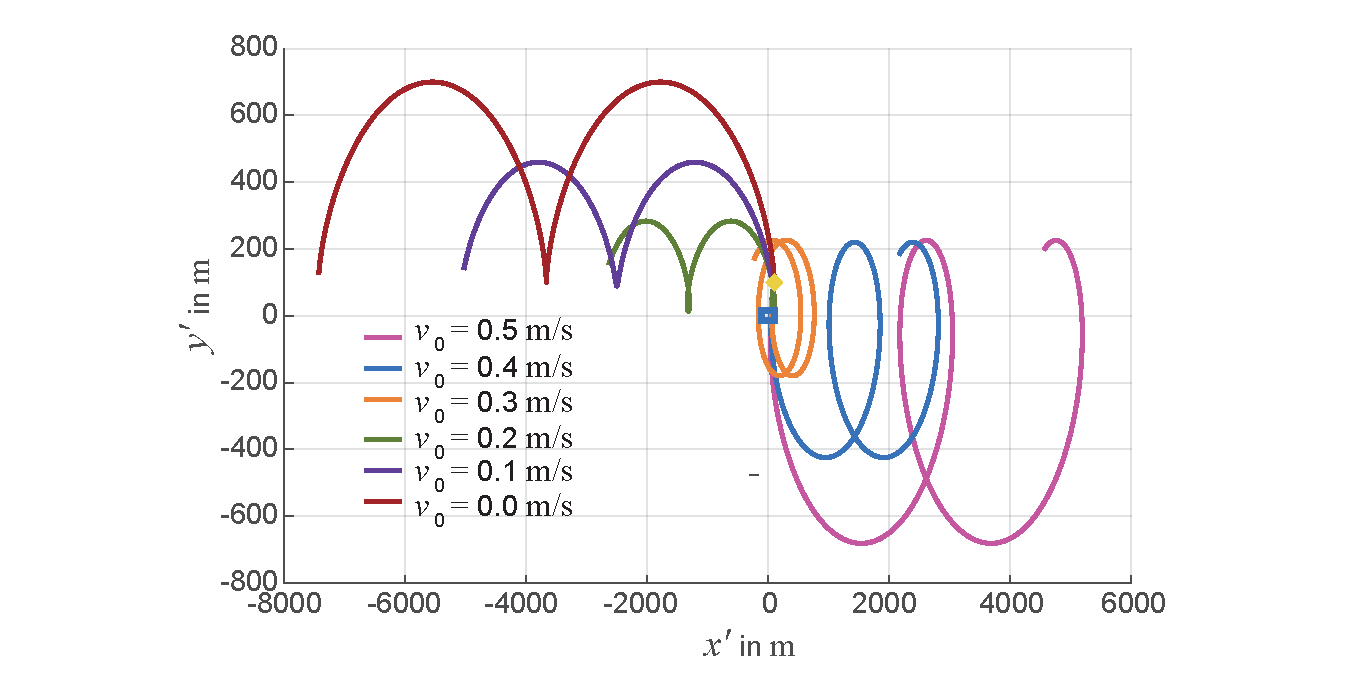
\includegraphics[width=\textwidth]{RendezvousAstronaut01.pdf} 
	\caption[Astronaut au�erhalb der ISS.]{Astronaut au�erhalb der ISS. Der Astronaut befindet sich initial bei $x_0'=y_0'=\SI{100}{\metre}$ und bewegt sich mit einer Anfangsgeschwindigkeit $v_0$ (also keine initiale Relativgeschwindigkeit zum Ziel, d.h. $\dot{x}_0'=\dot{y}_0=0'$) genau in Richtung auf die Station zu. Selbst bei $v_0=0$ entfernt sich der Astronaut mit der Zeit von der Raumstation. Dargestellt sind die L�sungen der Clohessy-Wiltshire-Gleichungen wie im \mscr~ \mladynref{Rendezvous01.m} im Detail ausgef�hrt.}
	\label{abb:adyn_rendezvous02}
\end{figure}

  \item[b)]
    Was passiert, wenn der Astronaut seinen R�ckkehrantrieb (englisch \textit{Return-Thruster}) mit einem Antriebsverm�gen von $\SI{1}{\metre\per\second}$ einsetzt?   
		Intuitiv \anf{zielt} der Astronaut mit seinem auf dem R�cksto�-Prinzip basierenden Thruster genau in Richtung ISS, also mit
    \begin{align*}
        \vec{v}_0 = 
        \begin{pmatrix}
            \dot{x}_0'\\
            \dot{y}_0'\\
            \dot{z}_0'
        \end{pmatrix}
        = \frac{1}{\sqrt{2}}
        \begin{pmatrix}
            1\\
            1\\
            0
        \end{pmatrix}
        \SI{}{\metre\per\second}\,.
    \end{align*}
    Leider wird durch die kombinierte Wirkung der Gezeiten und Coriolis-Kraft der Astronaut die ISS verfehlen, wie Gleichung \eqref{eq:adyn_rendez23} und \figref{adyn_rendezvous02} und \figref{adyn_rendezvous03}a zeigen.\\
    \item[c)]
    Wie muss der Astronaut beim Abfeuern seines Thrusters zielen, damit er die ISS sicher erreicht? \\
		$\dot{x}_0'$, $\dot{y}_0'$ ergeben sich aus \eqref{eq:adyn_rendez24}. Wir k�nnen noch eine kleine Eigengeschwindigkeit des Astronauten vor dem Starten des Thrusters mit $\vec{v}_\text{vor} = \lk\dot{x}_{\text{vor},0'}, \dot{y}_{\text{vor},0'}\rk$ annehmen und erhalten den richtigen Zielwinkel:
    \begin{align}
        \tan\lk\gamma\rk = \frac{\Delta v_y}{\Delta v_x} = \frac{\dot{y}_0' -\dot{y}_{\text{vor},0'}}{\dot{x}_0'- \dot{x}_{\text{vor},0'}} \,. \label{eq:adyn_rendez27}
    \end{align}
\end{enumerate}
In der Realit�t wird sich der Astronaut nat�rlich in kleinen Minisch�ben iterativ der ISS n�hern, doch auch daf�r gelten die abgeleiteten Formeln.

\begin{figure}[H]
	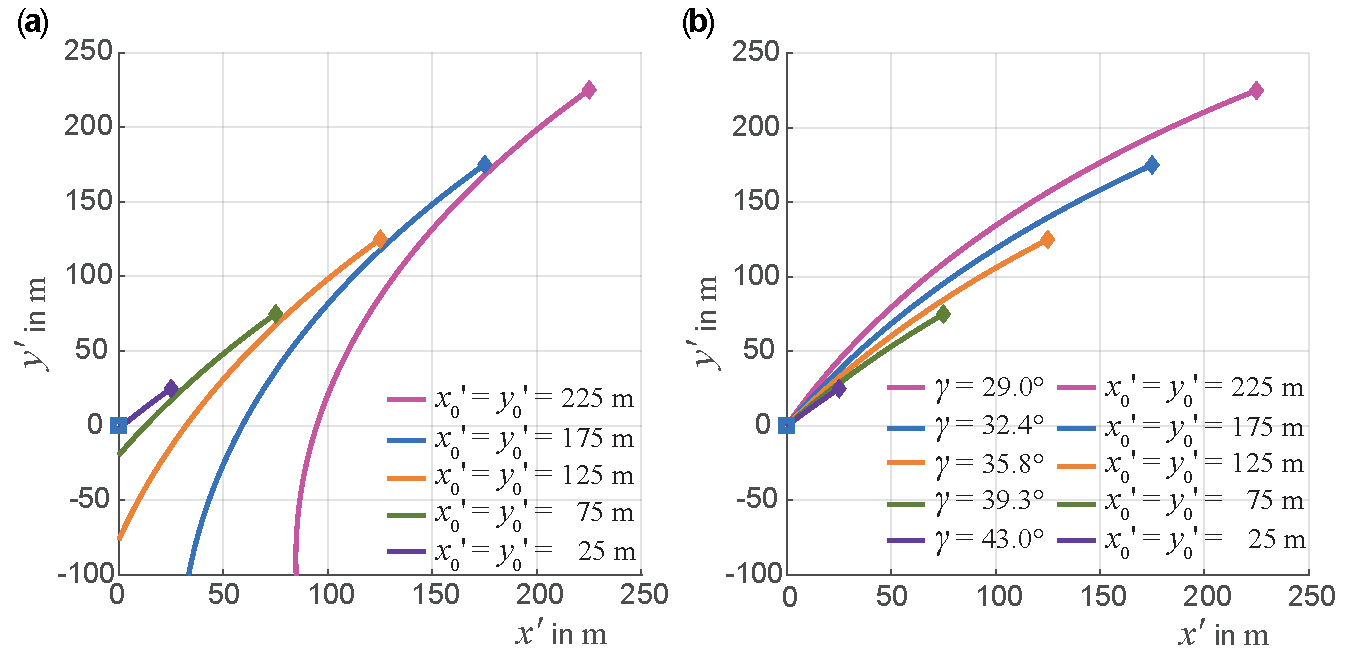
\includegraphics[width=\textwidth]{RendezvousAstronaut02.pdf} 
	\caption[Astronaut au�erhalb der ISS.]{Astronaut au�erhalb der ISS. \fa Der Astronaut befindet sich initial bei $x_0'=y_0'=\SI{25}{\metre} \ldots \SI{225}{\metre}$ und "`zielt"' mit seinem Antriebssystem  mit einer Anfangsgeschwindigkeit $v_0$ genau in Richtung auf die Station. L�sung der Hill-Gleichungen. \fb Der Astronaut befindet sich ebenfalls initial bei $x_0'=y_0'=\SI{25}{\metre} \ldots \SI{225}{\metre}$ und bewegt sich mit einem optimierten Zielwinkel $\gamma$ der Richtung Anfangsgeschwindigkeit von $v_0 = \SI{1}{\metre\per\second}$ auf die Station zu (L�sung der Clohessy-Wiltshire-Gleichungen\index{Clohessy-Wiltshire-Gleichungen}). Offensichtlich wird der Astronaut erst bei Entfernung von kleiner als 50 m bei direkter Anzielung der Station auch bei dieser wirklich ankommen. Die Rechnungen sind im \mscr~ \mladynref{Rendezvous02.m} im Detail ausgef�hrt.}
	\label{abb:adyn_rendezvous03}
\end{figure}

\label{bsp:adyn_stranded_astronaut}
\end{example}
%BEISPIEL %%%%%%%%%%%%%%%%%%%%%%%%%%%%%%%%%%%%%%%%%%%%%%%%%%%%%%%%%%%%%%%%%%%%%%%%%%%%%%%%%%

\subsection{Rendezvous Space Shuttle und ISS}\label{kap:adyn_rendezvous_ISS}

Ganz analog zu den Rechnungen im vorhergehenden Kapitel kann man das Weltraum-Rendezvous von einem Raumtransporter und der ISS berechnen. 
Wenn zwei Raumschiffe vor einer Kopplung f�r l�ngere Zeit in einem konstanten Abstand fliegen sollen, ist dies ohne st�ndigen Treibstoffverbrauch nur m�glich, wenn sich beide in der gleichen Umlaufbahn befinden. Ist dies nicht der Fall,  wird der Verfolger vom Ziel aus gesehen eine Ellipsenbahn (\bzw ellipsen�hnliche Bahn) beschreiben, die man sich leicht �ber die Berechnung im Inertialsystem aus den Kepler-Bahnen beschaffen kann. Dabei muss man ber�cksichtigen, dass das Koordinatensystem $\vec{\Sigma}'$ in der Zeit mitgedreht werden muss, denn die $y'$-Achse soll ja immer radial nach au�en zeigen.
Zur Berechnung der von der ISS beobachteten Bahnen �ber die Hill- \bzw CW-Gleichungen muss man neben den Anfangskoordinaten $\vec{r}_0,\, \vec{R}_0$ auch die Anfangsgeschwindigkeiten $\vec{v}_0,\, \vec{V}_0$, sowie deren Umrechnung in das mitbewegte \KOS\ der ISS (des Ziels) kennen. 
\begin{figure}[H]
	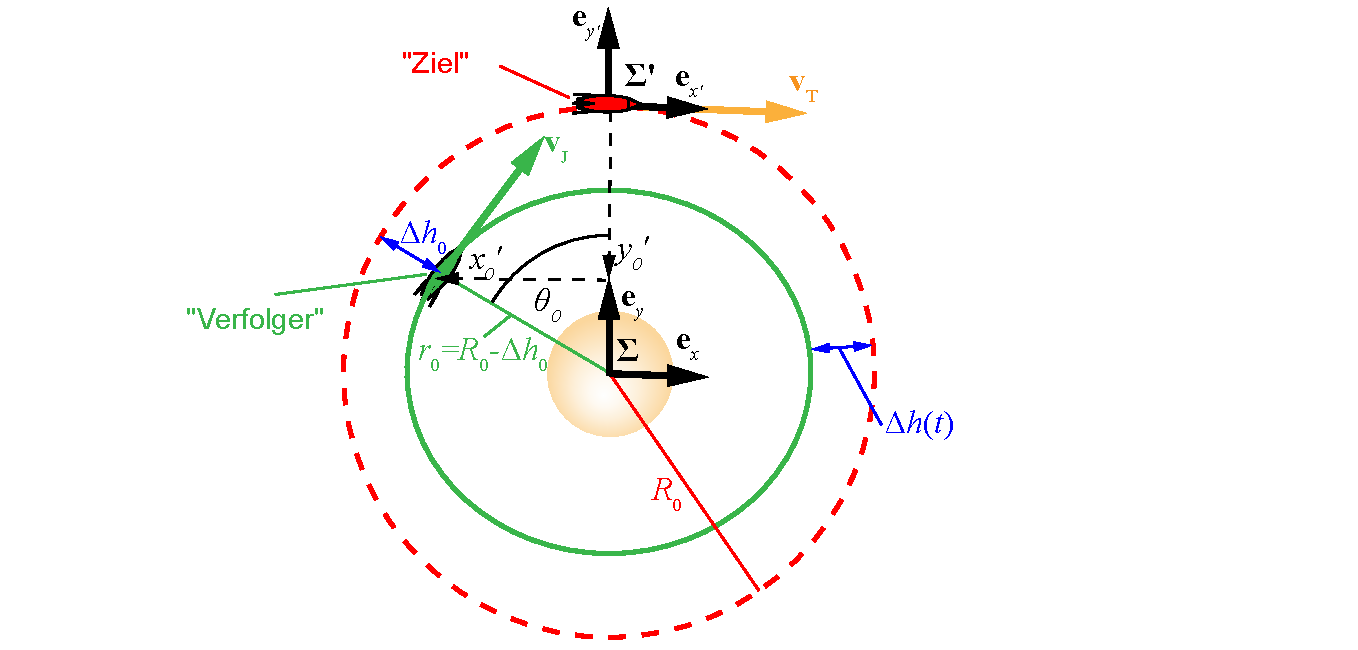
\includegraphics[width=\textwidth]{RendezvousKOS02.pdf} 
	\caption[Koordinatensysteme f�r Rendezvous in der Umlaufbahn.]{Koordinatensysteme f�r Rendezvous in der Umlaufbahn. Wir nehmen eine Bewegung der beiden Raumschiffe in der $x$-$y$-Ebene an. Die $z$-Achse zeigt aus der Papierebene heraus. F�r das Ziel wird vereinfachend eine Kreisbahn angenommen, der Verfolger befindet sich auf einer elliptischen Bahn. Ebenfalls wurde vereinfachend angenommen, dass zum Zeitpunkt $t=0$ die Achsen $\veceY,\, \vecpeY$ in die gleiche Richtung zeigen und $\veceY$ auch zum Perig�um der Bahn des Verfolgers.}
	\label{abb:adyn_rendezvousKOS02}
\end{figure}
Die Situation ist in \figref{adyn_rendezvousKOS02} gezeigt. Man liest f�r die Anfangsbedingungen ab:
	\begin{align}
	\begin{split}
		\vec{r}_0 &= x_0\, \veceX + y_0\,\veceY \,, \\
		\vec{R}_0 &= (0,R_0)\,, \\
		\vec{r}_0' &= x_0'\, \vecpeX + y_0'\,\vecpeY \,.
		\end{split} \label{eq:adyn_rendez28}
	\end{align}
Die beiden Vektoren $\vec{R}_0,\,\vec{r}_0$ bilden einen Winkel $\theta_0$, der sich mit $\Delta h_0 =\Delta h(t_0)$ aus
	\begin{align}
		\sin\theta_0 &= -\frac{x_0'}{R_0-\Delta h_0} ~~~\text{\bzw}~~~ \cos\theta_0 = -\frac{R_0+y_0'}{R_0-\Delta h_0}\, \label{eq:adyn_rendez29}
	\end{align}
bestimmen l�sst. F�r die Anfangsgeschwindigkeiten finden wir:
	\begin{align}
	\begin{split}
		\vec{V}_0 \,=\,&\dot{\vec{R}}_0 \,= \,R_0\,\omega_\text{T} \,\veceX\,,\\
		\vec{v}_0 \,=\,&\dot{\vec{r}}_0 \,= \,v_{\text{J},0} \lk \cos\theta_0\,\veceX + \sin\theta_0\,\veceY \rk\,.\\
	\end{split}  \label{eq:adyn_rendez30}
	\end{align}
Befindet sich der Verfolger auch auf einer Kreisbahn mit dem Radius $R_0-\Delta h_0$, dann ist $ v_{\text{J},0} = \omega_\text{J}\,(R_0-\Delta h_0)=\sqrt{G m_\text{M}/(R_0-\Delta h_0)}$, ansonsten bestimmt sich $v_{\text{J},0}$ aus der L�sung der Kepler-Gleichung \bzw der \gls{visvivaadyn} \eqref{eq:hm_vis-viva}. 
F�r einen solchen Fall nehmen wir eine Bahn des Verfolgers mit einer Exzentrizit�t $e$ und einer gro�en Halbachse $a=R_0$ an. Zum Zeitpunkt $t=0$ sollen sich Ziel und Verfolger bei $(0,0)\,\bzw (0,y_0')$ befinden. Dann ist 
\begin{align}
  \vec{v}_0 &= v_{\text{J},0} \,\veceX ~~~\text{mit}~~~v_{\text{J},0} = \sqrt{\frac{G\,m_\text{E}}{R_0}}\,\sqrt{\frac{1+e}{1-e}} \approx (1+e)\,R_0\,\omega_\text{T} \, \veceX \,. \label{eq:adyn_rendez30a}
\end{align}
Hat der Verfolger bereits im Inertialsystem eine Anfangsgeschwindigkeit $\vec{v}_0 \neq 0$, so m�ssen wir f�r die L�sung der Hill- \bzw die Nutzung der CW-Gleichungen, die sich daraus im mitbewegten \KOS\ $\vec{\Sigma}'$ ergebende Anfangsgeschwindigkeit $\vec{r}_0'$ kennen. Diese berechnet sich nach \eqref{eq:adyn_rendez04} zu:
	\begin{align}
		\dot{\vec{r}}_0' &= \dot{\vec{r}}'(t=0)= \dot{\vec{r}}_0 - \dot{\vec{R}}_0 - \vec{\omega}_0' \times \vec{r}'_0 = \vec{v}_0 - \vec{V}_0 - \vec{\omega}_0' \times \vec{r}'_0  \,. \label{eq:adyn_rendez31}
	\end{align}
Hierin ist $\vec{\omega}_0'$ der Rotationsvektor f�r die Drehung des mitbewegten Koordinatensystems, welches sich mit der Bewegung des Ziels so dreht, dass die $\vecpeY$-Achse immer radial nach au�en zeigt.

\begin{figure}[H]
	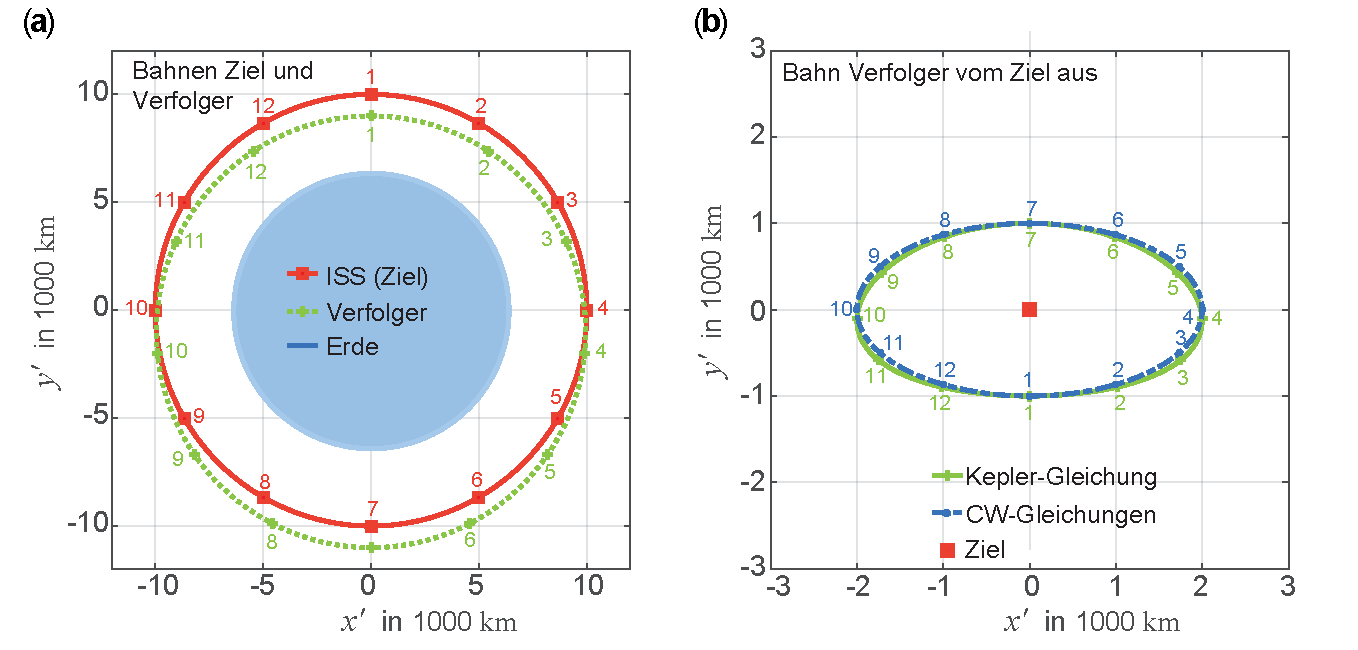
\includegraphics[width=\textwidth]{Raumschiff2Orbits.pdf} 
	\caption[Zwei Raumschiffe in unterschiedlichen Umlaufbahnen.]{Zwei Raumschiffe in unterschiedlichen Umlaufbahnen.\fa Bahnen von Ziel und Verfolger im Inertialsystem. \fb Bahn Verfolger von Ziel aus. L�sungen nach der Kepler-Gleichung mit Drehung des mitbewegten Koordinatensystems des Ziels (gr�n) und CW-L�sung (blau) im Vergleich. F�r die Bahn des Ziels wurde $R_0 = \SI{10000}{\kilo\metre}$ angenommen, die Bahn des Verfolgers habe eine Exzentrizit�t von $e=0.1$ und die gro�e Halbachse $a=R_0$. Es wurden 12 Zeitpunkte des Umlaufs gekennzeichnet. Die erkennbaren Abweichungen der exakten L�sungen nach der Kepler-Gleichung von der CW-L�sung resultieren aus der Tatsache, dass die Linearisierungsbedingung f�r die CW-Gleichung bei den vorliegenden Parametern nicht mehr erf�llt ist. (Siehe \mscr~ \mladynref{Rendezvous03.m} nach \cite{Carroll2019}) }
	\label{abb:adyn_rendezvous04}
\end{figure}

In unserem Fall (der Bewegung des Ziels im Uhrzeigersinn) k�nnen wir mit
	\begin{align}
		\vec{\omega}_0' &= -\omega_\text{T}\,\vecpeZ = -\omega_\text{T}\,\veceZ ~~~\text{und} ~~~\omega_\text{T} = \sqrt{\frac{G\,m_\text{E}}{R_0{}^3}}  \label{eq:adyn_rendez32}
	\end{align}
das Kreuzprodukt $\vec{\omega}_0' \times \vec{r}'_0$ in \eqref{eq:adyn_rendez31} berechnen zu:
\begin{align}
 	\dot{\vec{r}}_0' &= \sqrt{\frac{G\,m_\text{E}}{R_0}}\, \lek \sqrt{\frac{1+e}{1-e}}-1+e \rek\, \vecpeX \approx 2e\,R_0\,\omega_\text{T}\,\vecpeX\,. \label{eq:adyn_rendez34}
\end{align}
\figref{adyn_rendezvous04} zeigt die berechnete Bahn des Verfolgers vom Ziel aus betrachtet. F�r die CW-L�sung wurde die N�herung aus \eqref{eq:adyn_rendez34} verwendet, in \probref{adyn_rendezvous01} ist die Rechnung dann f�r Werte der ISS ausgef�hrt.
Wir wollen jetzt noch annehmen, dass die beiden Raumschiffe auf (ann�hernd) gleiche Bahn gebracht worden sind (in \figref{adyn_rendezvousKOS01} \bzw \figref{adyn_rendezvousKOS02} bedeutet das $y_0'=0$) und wollen absch�tzen, ab welchem Abstand $\Delta x'$ die Steuerung manuell direkt nach Sicht erfolgen kann.
Wir starten dazu mit der CW-Gleichung \eqref{eq:adyn_rendez14c} f�r $y'(t)$ und den Anfangsbedingungen $y_0' = 0$ und $\dot {y}_0'=0$ und nehmen wiederum eine Geschwindigkeit 
von $v_0=\dot{x}_0=\SI{1}{\metre\per\second}$ an. Es ergeben sich dann f�r die Koordinate $y'$ nach der Flugzeit $t\approx 100 \ldots 200 \mathrm{s}$ in der N�herung $\omega_0\,t \ll 1$ 
\begin{align}
	y'(t) = \frac{2\,\dot {x}_0'}{\omega_0}\,\frac{\lk \omega_0\,t\rk^2}{2} = \dot {x}_0'\,\omega_0\,t^2\,.\label{eq:adyn_rendez41}
\end{align}
Bei einem Anflug in direkter Sichtlinie muss aber die Docking-Einrichtung auf $y'(t) = \Delta d \approx \SI{2}{\metre}$ genau getroffen werden, womit sich aus
\eqref{eq:adyn_rendez41} mit $t=x_0'/\abs{\dot{x}_0'}$ der maximale Abstand $\Delta x'$ ergibt, bis zu welchem ein solcher Direktanflug manuell nach direkter Sichtlinie erfolgen kann (\figref{adyn_rendezvous04a}):
\begin{align}
	\Delta x' = \sqrt{\frac{\Delta d\, \abs{\dot{x}_0'}}{\omega_0}} \leq \SI{40}{\metre} \,.\label{eq:adyn_rendez42}
\end{align}
\begin{figure}[H]
	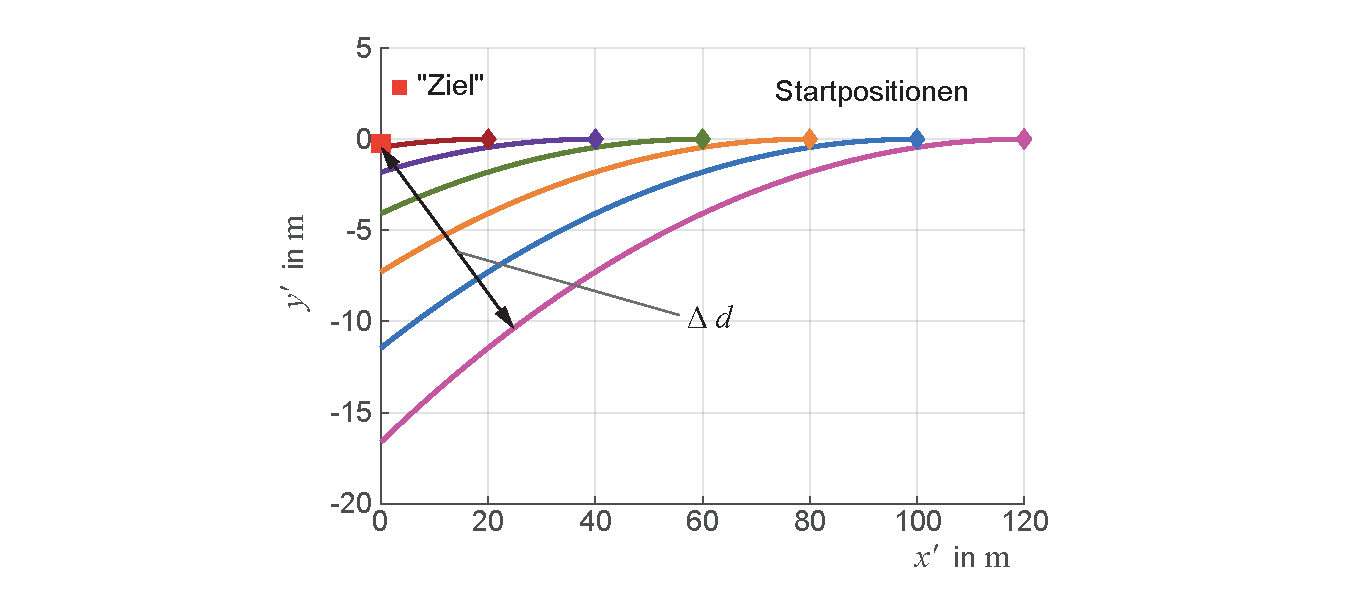
\includegraphics[width=\textwidth]{DirektAnflugISS.pdf} 
	\caption[Trajektorien eines Raumtransporters bei Anflug.]{Trajektorien eines Raumtransporters f�r verschiedene Anfangspunkte des Rendezvous-Man�vers (Anflug unter Schub in direkter Sichtlinie). Eingezeichnet ist auch der erreichte Endabstand $\Delta d$ (des jeweiligen Anflugs von $x_0'$) vom Zentrum der Docking-Vorrichtung f�r eine Anfangsgeschwindigkeit von $v_0 =  \SI{1}{\metre\per\second}$. (Nach \cite{Carroll2019}, siehe \probref{adyn_rendezvous01} \bzw \mscr~\mladynref{Rendezvous04.m})} \label{abb:adyn_rendezvous04a}
\end{figure}

\subsection{Wiederankopplung LM und CSM von Apollo 11}\label{kap:adyn_rendezvous_apollo11}

Ein besonders interessanter und zugleich f�r die erste bemannte Mondlandung extrem erfolgskritischer Fall eines Weltraum-Rendezvous war die Wiederankopplung der Mondf�hre von Apollo 11 (\gls{LM}\index{LM} "`The Eagle"', kurz: LM) nach der erfolgreichen Mondlandung mit den Astronauten Armstrong\footnote{Neil Alden Armstrong (1930--2012) war ein US-amerikanischer Testpilot und Astronaut. Er war Kommandant von Apollo 11 und betrat am 21. Juli 1969 als erster Mensch den Mond.}\indexp{Armstrong, Neil Alden} und Aldrin\footnote{Buzz Aldrin (geb. 1930)\indexp{Aldrin, Buzz} ist ein ehemaliger US-amerikanischer Astronaut, der im Rahmen der Apollo-11-Mission kurz nach Neil Armstrong als zweiter Mensch den Mond betrat.} an das Mutterschiff (\gls{CSM}\index{CSM}, kurz: CSM) mit dem Piloten Collins\footnote{Michael Collins (1930--2021) war ein US-amerikanischer Astronaut und umkreiste als Pilot des CSM einsam den Mond, w�hrend Armstrong und Aldrin die Mondoberfl�che betraten.}\indexp{Collins, Michael}. Details dieses Flugabschnitts sind in dem sehr lesenswerten Apollo Flight Journal \cite{Apollo11FJ} beschrieben.\\
Wir wollen den finalen Flugabschnitt des LM zwischen dem Zeitpunkt der \gls{TPI}\index{TPI} (TPI-Burn) und dem Bremsman�ver \gls{TPF}\index{TPF} (TPF) modellieren, vgl.~\figref{adyn_rendezvous05}.\footnote{Die vorhergehenden Flugabschnitte kann der Leser leicht mit dem Wissen aus dem \kap{adyn_maneuvers} nachvollziehen.}
Zum Zeitpunkt des TPI war das LM auf einer \ca 28 km tieferen Bahn als das CSM, \dh $y_0'=y_\text{LM}'\approx -\SI{28}{\kilo\metre}$. Der direkte Abstand zwischen LM und CSM betrug zu diesem Zeitpunkt \ca $\SI{56}{\kilo\metre}$, womit das CSM unter einem H�henwinkel von $\theta_0 = 26.5\degree$ vom LM aus "`gesehen"' wurde.\\

\begin{figure}[H]
	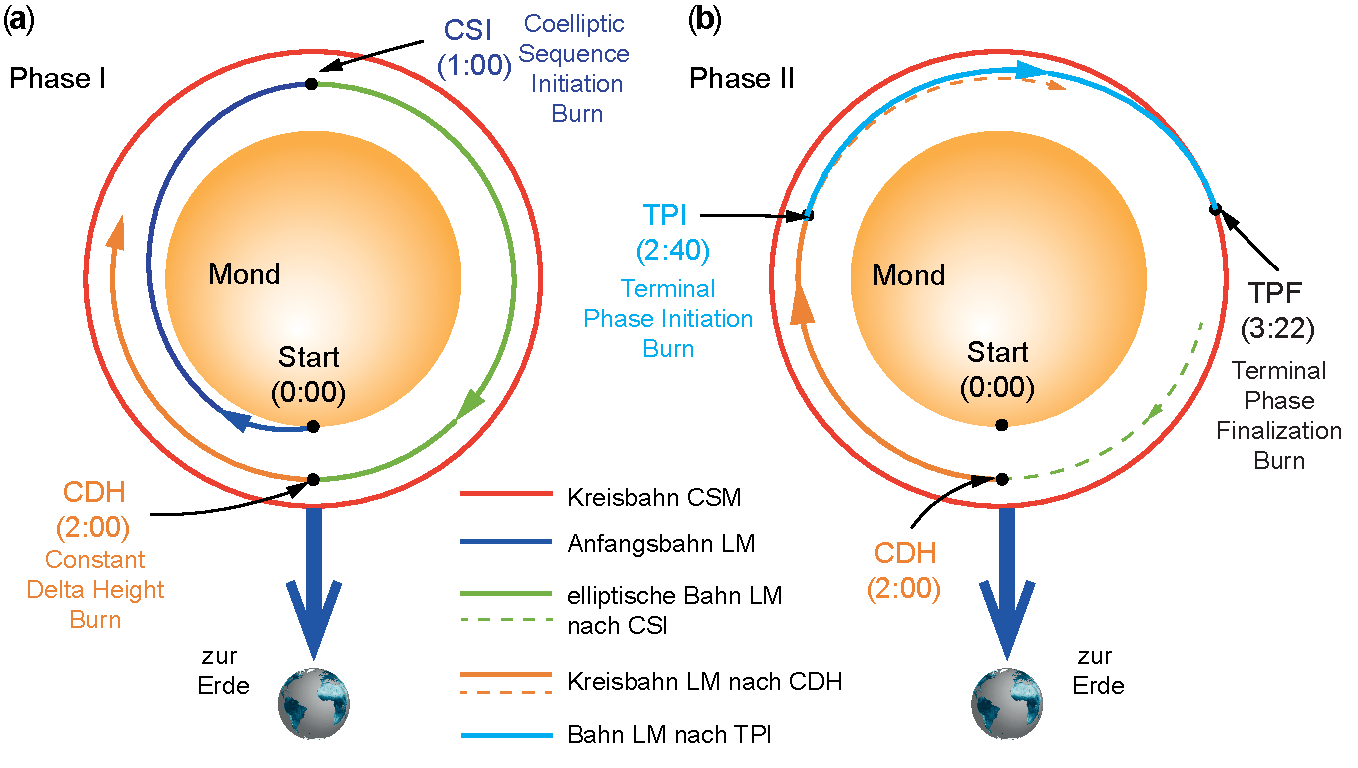
\includegraphics[width=\textwidth]{Apollo11LMCSMRendezvous.pdf} 
	\caption[Rendezvous von CSM und LM von Apollo 11.]{Rendezvous von CSM und LM von Apollo 11. \fa Phase I: Der Flug zum CSM begann mit dem Start des LM von der Mondoberfl�che und den Transfer in eine elliptische Bahn von $\SI{87.6}{} \,\mathrm{x}\, \SI{17.6}{\kilo\metre}$. %(\bzw  47.3 x 9.5 Nautische Meilen (die Ma�einheit der NASA)) 
	Nach einer Stunde hat das LM den apolunaren Punkt erreicht und kommt durch einen sogenannten CSI-Burn (\gls{CSI}) auf eine kreisf�rmigere Bahn von $\SI{92.5}{} \,\mathrm{x}\, \SI{85.0}{\kilo\metre}$. %(\bzw  50 x 46 Nautische Meilen)
	Durch einen weiteren Burn (CDH) erreicht das LM eine Bahn mit konstanter H�he und ist damit in einem konstanten H�henabstand von \ca $\SI{28}{\kilo\metre}$ zum CSM.
	%(\bzw  15 Nautischen Meilen)
  \fb Nach weiteren 40 Minuten erfolgt der so genannte TPI-Burn (\gls{TPI}), welche das LM auf die finale Rendezvous-Bahn bringt. 
%Nach diesem Burn fliegt das LM in einer nahezu geraden Linie in Bezug auf das feste KOS\ der Sterne auf das CSM zu. Tats�chlich haben die Astronauten die Fixsterne als visuelle Referenz zur Korrektur der Ann�herung benutzen k�nnen, da sich das LM auf der Nachtseite des Mondes befand. Die finale Phase der Ann�herung und das Bremsman�ver (TPF) erfolgten dann bei Tageslicht. %Zwischen TPI und TPF gab es zwei weitere kleinere Kurskorrekturen, die wir hier aber nicht weiter ber�cksichtigen m�ssen.
	(Nicht ma�st�bliche Zeichnung nach dem NASA Flight Journal von Apollo 11.)}
	\label{abb:adyn_rendezvous05}
\end{figure}

Wir haben in \kap{adyn_rendezvous} gelernt, dass f�r einen Burn zum direkten Anflug ein anderer Zielwinkel $\gamma$ angenommen werden muss als der direkte Sichtwinkel $\varphi_0 =\arctan({y_0'/x_0'})$. Um diesen Winkel $\gamma$ mit den CW-Gleichungen \eqref{eq:adyn_rendez27} zu berechnen, brauchen wir die Anfangsgeschwindigkeit $\vec{v}_{\text{LM},0}$ des LM im CSM-\KOS\ vor dem Burn. Wir haben diese bereits im vorhergehenden \kap{adyn_rendezvous_ISS} hergeleitet. Wir benutzen das Ergebnis hier, jetzt aber f�r zwei kreisf�rmige Bahnen (f�r CSM und LM). Dann folgt aus Gleichung \eqref{eq:adyn_rendez34} eine Geschwindigkeit des LM vor dem Burn zu:
\begin{align}
	\vec{v}_{\text{LM},0} = \lk \omega_\text{LM} - \omega_\text{CSM} \rk \, \lek \lk R_\text{CSM} + y_0' \rk \, \vecpeX - x_0 \, \vecpeY \rek \,. \label{eq:adyn_rendez43}
\end{align}
Die $x_0',\, y_0'$ ergeben sich aus einfacher geometrischer Betrachtung aus \figref{adyn_rendezvousKOS02} und die Kreisfrequenzen der Umlaufbahnen sind gegeben durch:
\begin{subequations}
	\begin{align}
		\omega_\text{CSM} &= \sqrt{\frac{G\,m_\text{M}}{R_\text{CSM}{}^3}} \approx \SI{8.8e-4}{\radian\per\second} \,,\\
		\omega_\text{LM} &= \sqrt{\frac{G\,m_\text{M}}{R_\text{LM}{}^3}} = \sqrt{\frac{G\,m_\text{M}}{\lk R_\text{CSM} - \Delta h\rk^3}} \approx \SI{9.0e-4}{\radian\per\second}\,, \label{eq:adyn_rendez44}
	\end{align} 
\end{subequations}
worin $m_\text{M}$ die Masse des Mondes und $R_\text{CSM},\, R_\text{LM}$ die Bahnradien der beiden Raumschiffe vor dem TPI sind. Wir k�nnen Gleichung \eqref{eq:adyn_rendez43} f�r $x_0',\, y_0' \ll R_0$ entwickeln, indem wir f�r $\omega_\text{LM}$ n�herungsweise $\omega_\text{LM} \approx \sqrt{\lk G\,m_\text{M}\rk/\lk R_\text{CSM} - y_0'\rk^3} $ schreiben und erhalten dann aus \eqref{eq:adyn_rendez43}
\begin{align}
	\vec{v}_{\text{LM},0} = \begin{pmatrix} v_{\text{LM},0,x'} \\ v_{\text{LM},0,y'} \end{pmatrix}
	= -\frac{3}{2}\,\omega_\text{CSM} \, y_0' \,\begin{pmatrix} -x_0'/R_0 \\ 1 + y_0'/R_0 \end{pmatrix} \begin{pmatrix} \vecpeX \\ \vecpeY \end{pmatrix}\,.
	\label{eq:adyn_rendez46}
\end{align}
Damit haben wir alle Gr��en, um aus den CW-Gleichungen den Geschwindigkeitsbedarf f�r das TPI-Man�ver, die Richtung des TPI-Burn und die finale Trajektorie nach dem TPI zu berechnen.
Das Ergebnis der Rechnungen haben wir f�r verschiedene $y_0'$ in \figref{adyn_rendezvous06} dargestellt. Man berechnet f�r den Geschwindigkeitsbedarf des TPI-Burn 
\begin{align}
	\Delta v = \sqrt{\lk \dot{x}_0' - v_{\text{LM},0,x'}\rk^2 + \lk \dot{y}_0'-v_{\text{LM},0,y'}\rk^2}\,,\label{eq:adyn_rendez47}
\end{align}
wobei sich die $\dot{x}_0',\,\dot{y}_0'$ aus \eqref{eq:adyn_rendez24} berechnen. F�r die drei F�lle aus \figref{adyn_rendezvous06} ergeben sich Geschwindigkeitsbedarfe von $\Delta v = 8.0 \ldots \SI{6.9}{\metre\per\second}$ und ein Zielwinkel des Burn von $\gamma= 19.8\degree$ (nicht zu verwechseln mit dem Abflugwinkel $\alpha$), was gut mit der NASA Planung von $\Delta v = \SI{7.5}{\metre\per\second}$ �bereinstimmt. Man erkennt auch aus \figref{adyn_rendezvous06}, dass selbst bei Verpassen des optimalen Zeitpunktes des TPI-Burn (\dh der richtigen H�he $y_0'$) die Burn-Richtung und auch die Gr��e von $\Delta v$ relativ unkritisch sind f�r den Erfolg des Man�vers, was sicher etwas vom Stress der Astronauten wegnahm.
\begin{figure}[H]
	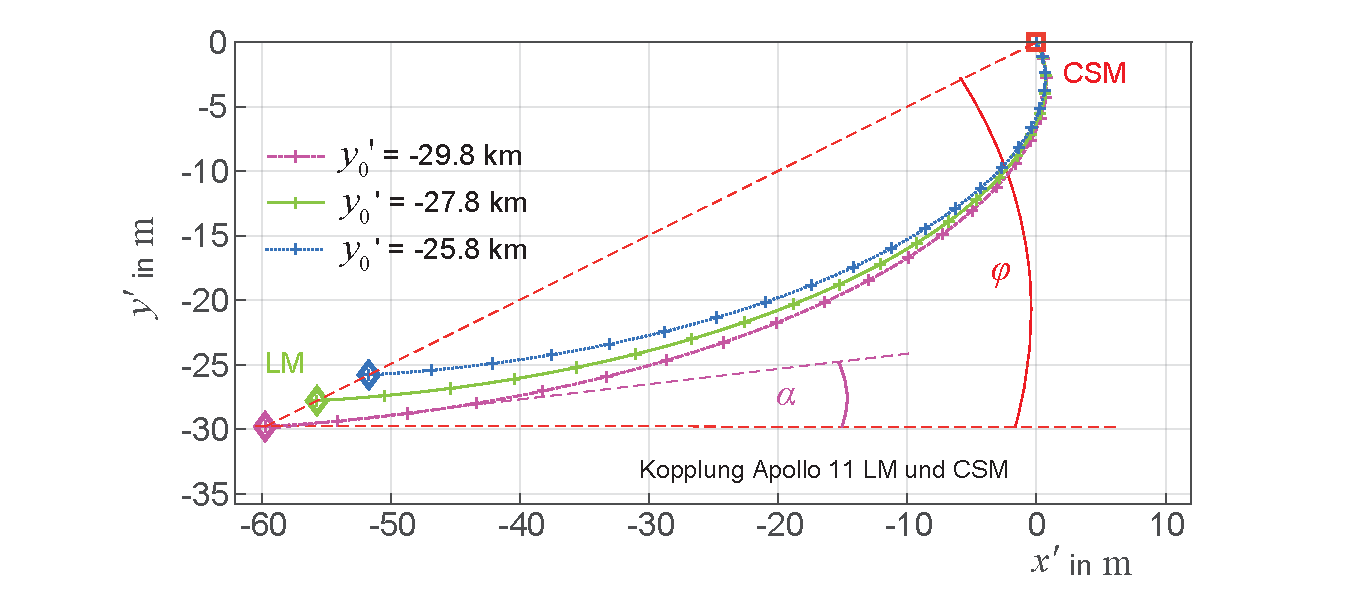
\includegraphics[width=\textwidth]{Apollo11LMCSMTrajektorie.pdf} 
	\caption[Trajektorien des LM im Anflug auf das CSM von Apollo 11.]{Trajektorien des LM im Anflug auf das CSM von Apollo 11 f�r verschiedene H�hen des TPI-Burn. Siehe \probref{adyn_rendezvous02} \bzw \mscr~\mladynref{LMCSMApollo11.m}.}
	\label{abb:adyn_rendezvous06}
\end{figure}
Wir m�chten noch erw�hnen, dass nach der erfolgreichen Kopplung und dem Umstieg der Astronauten vom LM ins CSM das LM wieder abgesprengt wurde. Das wohl mit bedeutsamste Fahrzeug der Menschheitsgeschichte war damit sich selbst \bzw dem Gravitationsfeld des Mondes �berlassen. Bis heute konnte man keinen Einschlagkrater des LM auf dem Mond finden, so dass man davon ausgehen muss, dass der \textit{"`Eagle"'}  noch immer den Mond umkreist. Wer sich Modellrechnungen f�r eine m�gliche Bahn des LM anschauen will, dem seien die Referenzen \cite{Khan2021} und \cite{meador2021} empfohlen. Letztere eignet sich auch f�r einen Einstieg in das von der NASA der Allgemeinheit zur Verf�gung gestellte GMAT-Paket \url{software.nasa.gov/software/GSC-17177-1}, in welchem auch sehr leistungsf�hige \matlab-Programme f�r die Astrodynamik und Himmelsmechanik zu finden sind.




 
\section{Start aus der Erdatmosph�re und Wiedereintritt}\label{kap:adyn_launch_reentry}

\subsection{Kr�fte im erdnahen Weltall}\label{kap:adyn_forces}

Zum Abschluss der Astrodynamik wollen wir uns mit Situationen besch�ftigen, in denen neben der Gravitationskraft weitere Kr�fte eine Rolle spielen. Das ist insbesondere bei Starts von der Erdoberfl�che, Bahnen in niedriger H�he und nat�rlich beim Wiedereintritt in die Erdatmosph�re der Fall. \\
In den meisten F�llen wird man die Bewegungsgleichung nur numerisch integrieren k�nnen, wir wollen aber in einigen F�llen auch N�herungsformeln angeben. \\
Zun�chst untersuchen wir die zur Gravitation der Erde (die als Zentralkraft angenommen wird) zus�tzlich auftretenden Kr�fte, um dann die jeweiligen relevanten Kr�fte bei der Berechnung von Start, Wiedereintritt in die Erdatmosph�re \bzw in Flug in niedrigen Orbits zu ber�cksichtigen. 

\subsubsection{Atmosph�rische Reibung \index{Drag}\index{Reibung!atmosph�rische}}\label{kap:adyn_drag}

Die atmosph�rische Reibung stellt die gr��te nicht-gravitative St�rung f�r Satelliten und Raumsonden bei Start und Wiedereintritt sowie Fl�gen in extrem geringen Flugh�hen dar. Die genaue Modellierung der atmosph�rischen Reibung ist aber nicht ganz einfach, da \ia die Eigenschaften der Atmosph�re in den verschiedenen H�henbereichen nicht ausreichend genau bekannt sind und auch die genaue Wechselwirkung der atmosph�rischen Teilchen mit der Form und Oberfl�che des Raumschiffs stark variiert. \\
Wir werden deshalb auf das uns aus Band I bereits bekannte einfache Kraftmodell der Newtonschen Reibung zur�ckgreifen. 
Nach diesem beschreiben wir die atmosph�rische Reibung (Englisch \textit{\gls{drag}}\index{Drag|textbf}) mit:
\begin{align}
    \vec{F}_\text{D} = -\frac{1}{2}\,c_\text{D}\,A\,\varrho\,v_\text{R}{}\,\dot{\vec{r}}\,. \label{eq:adyn_forces01}
\end{align}
Hierin ist $c_\text{D}$ der atmosph�rische Reibungskoeffizient, der typischerweise im Bereich von $\SI{1.5}{}\ldots\SI{3.0}{}$ liegt, $A$ die effektive Querschnittsfl�che des Raumschiffs, $\varrho$ die (h�henabh�ngige) Dichte der Atmosph�re und $v_\text{R}$ der Betrag des momentanen Geschwindigkeitsvektors~$\dot{\vec{r}}$. F�r die Dichte werden in der Astrodynamik verschiedene Modelle verwendet, im einfachsten Fall kann $\varrho$ nach der barometrischen H�henformel \index{H�henformel!barometrische|textbf} mit 
\begin{align}
    \varrho = \varrho_0\,\e^{-\frac{h}{H_0}} \label{eq:adyn_barom_h_fomulae}
\end{align}
angegeben werden,
worin $H_0$ und $\varrho_0$ f�r die Standardatmosph�re \cite{ISA1976} durch
\begin{align}
    H_0= \frac{R\,T}{\tilde{M}_\text{L}\,g} = \SI{6.7}{\km}~~~\text{und}~~~\varrho_0 = \SI{1.752}{\kg\per\metre\cubed} \label{eq:adyn_barom_h_fomulae_zusatz}
\end{align}
gegeben sind. 
$R$ ist die universelle Gaskonstante $R= \SI{8.314}{\joule\per\K\per\mole}$, $T$ die gegebenenfalls h�henabh�ngige absolute Temperatur und $\tilde{M}_\text{L}$ ist die (mittlere) molare Masse der Luft $\tilde{M}_\text{L}=\SI{28.9e-3}{\kg\per\mole}$. Letztlich wird die Dichte noch von Faktoren wie der Einstrahlung der Sonne (die eine halbt�gliche Variation der Dichte bewirkt) und auch geomagnetischen Einfl�ssen abh�ngen, die Teilchendichte und -zusammensetzung beeinflussen.\footnote{Ein in der Astrodynamik weit verbreitetes Modell ist das Harris-Priester-Modell, das aber �ber den Umfang und Anspruch dieses Buches hinausgeht. Wir verweisen auf die weiterf�hrende Literatur \cite{Walter2018, Montenbruck2012}.} 
Wir werden f�r unsere grobe Absch�tzung \ia mit der barometrischen H�henformel oder der tabellierten Standardatmosph�re (US Standard Atmosphere Table \cite{ISA1976}) arbeiten, was f�r unsere Zwecke meist ausreichend ist.
Es sei noch darauf hingewiesen, dass die Atmosph�re neben dem Drag auch noch einen Auftrieb bewirken kann, den wir beim Wiedereintritt zu ber�cksichtigen haben, sonst aber vernachl�ssigen werden. 

\subsubsection{Strahlungsdruck \index{Strahlungsdruck}} \label{kap:adyn_strahlungsdruck}

Der Strahlungsdruck ist eine weitere St�rkraft. Sie wird hervorgerufen durch den Druck, den ein Strahl von Photonen auf einen K�rper aus�bt, wenn dieser auf die Oberfl�che des K�rpers trifft. Wir werden diese in der Elektrodynamik herleiten, hier geben wir nur die f�r die Astrodynamik relevante Beziehung an:
\begin{align}
    F_\text{Rad} = \frac{s_0}{c}\,\lk\frac{\au}{d}\rk^2 \label{eq:adyn_forces04}
\end{align}
mit $s_0 = \hat{s}_0\,\lek 1+0.034\,\cos\lk\frac{360\,n}{365.25}\rk\rek$ und $\hat{s}_0 = \SI{1376.6}{\W\per\square\metre}$ (Solarkonstante). Dabei sind $n$ die Nummer des Tages eines Jahres, $d$ der Abstand der Raumsonde zur Sonne und $\au$ wie �blich die astronomische Einheit.\\
Die tats�chlich auf ein Raumschiff ausge�bte Kraft des Strahlungsdrucks h�ngt von weiteren Faktoren ab, \zb der tats�chlichen Geometrie des Raumschiffs, der  Abschattung der Sonne durch andere Himmelsk�rper \ua Wir werden den Strahlungsdruck im weiteren nicht ber�cksichtigen, er ist bei Start und Wiedereintritt \ia gegen den Drag zu vernachl�ssigen, muss aber bei HEO-Satelliten und im interplanetaren Raumflug\footnote{Der Strahlungsdruck kann besonders im interplanetaren Raum auch zum Antrieb benutzt werden. Dazu werden Raumschiffe mit sogenannte Sonnensegeln, die die Solarstrahlung zum Antrieb des Raumschiffs nutzen, ausgestattet. In \cite{Bailer2021} wird die japanische Mission IKAROS behandelt, die mit einem solchen Antrieb im interplanetaren Raum unterwegs ist.} unbedingt ber�cksichtigt werden. 

\subsubsection{Gravitative St�rungen} \label{kap:adyn_gravity_pertubations}
Neben Drag und Strahlungsdruck gibt es auch St�rungen, die durch das nicht vollst�ndig sph�rische Gravitationsfeld hervorgerufen werden. Solchen St�rungen werden durch die Abweichung der Form der Erde von einer idealen Kugel oder vom Gravitationseinfluss anderer Planeten und Monde hervorgerufen. Wir sind diesen Kr�ften bereits mehrfach begegnet. Im Kapitel 1.5.6 in Band I hatten wir bei der Behandlung der Pr�zession der Erde und in diesem Band im \kap{Periheldrehung} bei der Perihelverschiebung des Merkurs bereits solche St�rungen ber�cksichtigt. \\
Die allgemeine Vorgehensweise zur Berechnung solcher St�rungen mit Hilfe der Potential\-theorie hatten wir ausf�hrlich bei der Theorie der Gezeiten in \kap{hm_gezeiten_Laplace} behandelt. Wir haben das reale, von der sph�rischen Symmetrie abweichende Gravitationspotential $U\lk \vec{r} \rk  = U(r,\, \phi,\,\lambda)$ nach \eqref{eq:hm_pot_theo07a} durch eine Entwicklung nach Kugelfl�chenfunktionen\index{Kugelfl�chenfunktionen} des Winkels der geozentrischen Breite $\phi$ beschrieben. Der Einfachheit halber haben wir Rotationssymmetrie angenommen (also keine Abh�ngigkeit von der L�nge $\lambda$) und brauchen deshalb nur die Entwicklung nach $\phi$ zu betrachten. In \eqref{eq:hm_pot_theo07a} hatten wir den Winkel~$\theta$ verwendet und deshalb bei den Legendre-Polynomen\index{Legendre-Polynome} $\PL n(\,\cos\theta)$ geschrieben.  Hier aber benutzen wir die geozentrische Breite $\phi=\frac{\pi}{2}-\theta$ , so dass sich ergibt: 
\begin{align}
    \frac{1}{m}\,U\lk r,\phi\rk =-\frac{M\,G}{r}\,\lk 1-\sum\limits_{n-2}^\infty\,J_n\,\lk\frac{R_0}{r}\rk^n\,\PL n\,\lk\sin\phi\rk\rk \,.\label{eq:adyn_forces05} 
\end{align}
Die St�rterme $J_n$ in \eqref{eq:adyn_forces05} bestimmen sich aus der Form und Masseverteilung der Planeten und werden oft auch als zonale Harmonische\index{Harmonische!zonale} bezeichnet. Nehmen wir die f�r die meisten Himmelsk�rper g�ltige N�herung eines oblaten Rotationsellipsoids an, gilt:
\begin{align*}
    J_2 \gg J_n ~~~~ \forall\, n>2\,.
\end{align*}
F�r die Erde gilt beispielsweise $ |J_2| = \SI{1.08e-3}{} \: \gg \:|J_4| = \SI{1.62e-6}{}$, 
so dass es f�r unsere Zwecke gen�gt, nur $J_2$ bei der Berechnung von \eqref{eq:adyn_forces05} zu ber�cksichtigen. 
Bei der Behandlung der Gezeiten in \kap{hm_gezeiten} hatten wir auch gesehen, dass das Potential der Gezeitenkr�fte eine �hnliche mathematische Struktur aufweist, wie das Potential welches durch einen Rotationsellipsoiden erzeugt wird. Wir k�nnen daher annehmen, dass die Gezeitenkr�fte von Sonne und Mond �hnliche St�rwirkungen auf einen Erdorbit eines Satelliten hervorrufen, wie die St�rungen, die von der abgeplatteten Form der Erde herr�hren. \\
Tabelle \ref{tab:adyn_forces01} zeigt die relativen Gr��enverh�ltnisse der einzelnen St�rungen f�r eine Bahn $h=\SI{400}{\km}$ (ISS) und eine Bahn $h\approx\SI{40000}{\km}$ (GEO-Satellit).\\
Die Frage ist nun, wie die einzelnen St�rbeschleunigungen wirken. Da der Drag immer entgegen der Bewegungsrichtung wirkt, f�hrt er zu einer Geschwindigkeits�nderung und somit auch einer �nderung von Halbachse und Elliptizit�t der Bahn. Die zonalen Harmonischen $J_n$ und auch die Gravitationseinfl�sse von Sonne und Mond bewirken eine Drehung der Apsidenlinie \bzw Perig�umsverschiebung (\vgl \kap{Periheldrehung}) und eine Verschiebung des Knotens der Bahn. Abh�ngig von der Einstrahlcharakteristik der solaren Strahlung kann der Strahlungsdruck sowohl eine �nderung des Bahnradius als auch der Apsidenlinie bewirken.\\

\begin{table}[ht]
    \begin{center}
    \begin{tabular}{|C{4cm}|C{3cm}|C{3.0cm}|}
    \hline
    \rule{0pt}{3pt}& &  \\
      $\text{St�rung durch}$ & ISS/LEO-Satellit  & GEO-Satellit \\
    %\rule{0pt}{3pt}& &  \\
       & $h\approx\SI{500}{\km}$ & $h\approx\SI{40000}{\km}$ \\
    \rule{0pt}{3pt}& &  \\
    \hline
    %\rule{0pt}{3pt}& &   \\
    \rule{0pt}{6pt} Abplattung Erde $J_2$&$\SI{e-5}{}$ & $\SI{e-8}{}$ \vphantom{$I^{I^I}$} \\
    %\rule{0pt}{3pt}& &  \\
    \rule{0pt}{6pt} $\text{Gravitation Mond}$ &$\SI{e-9}{}$ & $\SI{5e-9}{}$ \\
    %\rule{0pt}{3pt}& &  \\
    \rule{0pt}{6pt} $\text{Gravitation Sonne}$ &$\SI{5e-10}{}$ & $\SI{2e-9}{}$ \\
    %\rule{0pt}{3pt}& &  \\
    \rule{0pt}{6pt} Abplattung Erde $J_4$&$\SI{e-8}{}$ & $\SI{1e-11}{}$ \\
    %\rule{0pt}{3pt}& &  \\
    \rule{0pt}{6pt} $\text{Strahlungsdruck}$ &$\SI{5e-8}{}$ & $\SI{5e-8}{}$ \\
    %\rule{0pt}{3pt}& &  \\
    \rule{0pt}{6pt} $\text{Drag}$ &$\SI{6e-8}{}$ & $\approx 0$ \\
    %\rule{0pt}{3pt}& &  \\
    \hline
    \end{tabular}    
    \end{center}
    \caption{Ungef�hre Gr��enordnungen von St�rbeschleunigungen (alle in $\SI{}{\km\per\square\second}$) auf Satelliten in verschiedenen H�hen �ber der Erde \cite{Montenbruck2012, Walter2018}.}
    \label{tab:adyn_forces01}
\end{table}
\subsection{Raketenstart von der Erde}\label{kap:adyn_launch}

Ein Raketenflug in eine erdnahe Umlaufbahn kann in drei Phasen unterteilt werden:
\begin{itemize}
	\item Start und die Schubphase, in der die Rakete mit dem Raumschiff auf eine Geschwindigkeit~$v_\text{f}$ bis zum �bergangspunkt (\gls{Brennschluss}) beschleunigt wird,
	\item die Bewegung auf einer freien Kepler-Trajektorie bis zum Erreichen des Apog�ums,
	\item den Burn mit $\Delta v$, der das Raumschiff auf die gew�nschte Zielumlaufbahn bringt.
\end{itemize}
Diese Phasen sind in \figref{adyn_launch01}a dargestellt. Wir weisen bereits hier darauf hin, dass man sich das Problem der R�ckkehr eines Raumschiffs zur Erde, insbesondere unter Ber�cksichtigung der Phase des Wiedereintritts in die Erdatmosph�re, als genau umgekehrt ablaufende Dynamik vorstellen kann (\figref{adyn_launch01}b). Wir werden das im \kap{adyn_reentry} genauer betrachten.

\begin{figure}[H]
\includegraphics[width=\textwidth]{PhasenStartvonErde.pdf}
\caption[Phasen eines Raketenflugs vom Start bis in eine Erdumlaufbahn.]{\fa Phasen eines Raketenflugs vom Start auf der Erdoberfl�che in eine Erdumlaufbahn. Der �bergangspunkt ist hier durch das Ende der Schubphase definiert. \fb Phasen eines Raketenflugs aus einem Erdorbit bis zur Landung auf der Erdoberfl�che. Der �bergangspunkt  ist hier durch den Eintritt in den sogenannten aerodynamischen Bereich (\kap{adyn_reentry}) definiert.}
\label{abb:adyn_launch01}
\end{figure}

In \figref{adyn_launch02} sind:
\begin{center}
\begin{tabular}{L{2cm}L{10cm}}
        \rule{0pt}{12pt}$\vec{F}_\text{S}, \vec{F}_\text{D}$, $\vec{F}_\text{A}$ & die Schubkraft, der \index{Drag}\textit{\glslink{drag}{Drag}} \bzw der Auftrieb,  \\
        \rule{0pt}{12pt}$\alpha$ & der Winkel zwischen Schub $\vec{F}_\text{S}$ und der Geschwindigkeit der Rakete $\vec{v}$, im Englischen \index{Angle of Attack}\textit{\glslink{AngleOfAttack}{Angle of Attack (AoA)}} genannt, \\
        \rule{0pt}{12pt}$\gamma$ & der Winkel zwischen der Geschwindigkeit $\vec{v}$ und dem lokalen Horizont, im Englischen \index{Flight Path Angle}\textit{\glslink{FlightPathAngle}{Flight Path Angle (FPA)}} $\gamma$ genannt,\\
         \rule{0pt}{12pt}$h, s$ & die H�he �ber der Erdoberfl�che \bzw  der zur�ckgelegte Weg der Sonde.\\
\end{tabular}
\end{center}

Wir berechnen nun unter Ber�cksichtigung der �u�eren Kr�fte die Aufstiegsbahn einer Rakete. Nach Tabelle \ref{tab:adyn_forces01} m�ssen wir f�r die Aufstiegsphase sicher den Drag einrechnen, alle anderen Kr�fte k�nnen wir im Bereich $R_\text{E} < r < R_\text{E} + h$ mit $h \leq \SI{100 }{\km}$ vernachl�ssigen. \\
Um die Bewegungsgleichungen aufzustellen, betrachten wir \figref{adyn_launch02}a. In vektorieller Form lauten diese im Erd-\KOS :
\begin{align}
      m_\text{R}(t)\,\ddot{\vec{r}} &= \vec{F}_\text{S} (t) + m_\text{R}(t)\,\vec{g}(\vec{r}) + \vec{F}_\text{D}(\dot{\vec{r}}, \vec{r}) + \vec{F}_\text{A}(\dot{\vec{r}}, \vec{r})  \,. \label{eq:adyn_launch_vec}
\end{align}

\begin{figure}[H]
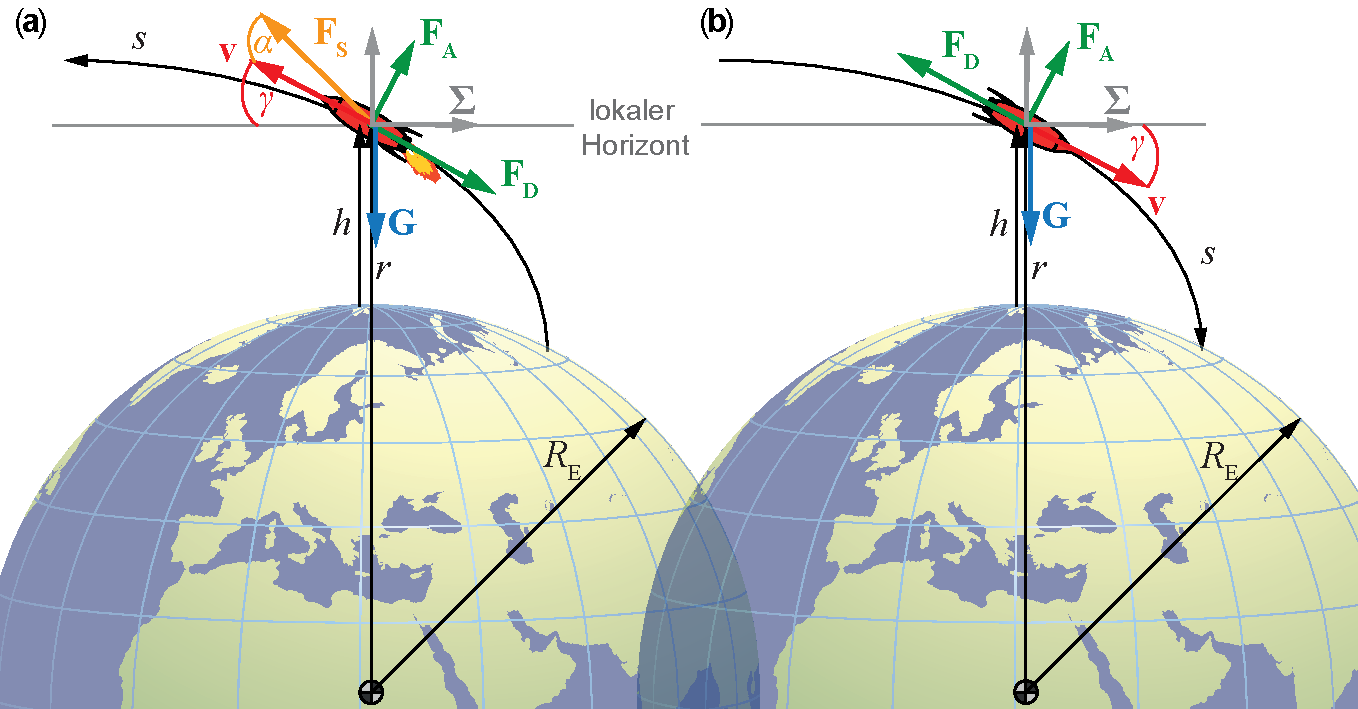
\includegraphics[width=\textwidth]{RaumflugstartErde.pdf}
\caption[Kr�fte beim Raketenstart von der Erdoberfl�che und beim Wiedereintritt.]{Zur Herleitung der Bewegungsgleichungen f�r den Raketenstart \bzw den Wiedereintritt in die Erdatmosph�re. \fa Kr�fte beim Raketenstart von der Erdoberfl�che. \fb Kr�fte beim Wiedereintritt in die Erdatmosph�re.}
\label{abb:adyn_launch02}
\end{figure}

Bei der Planung von realen Raumfahrtmissionen wird man \ia mit bekannten \bzw vorgegebenen  Gr��en $\vec{F}_\text{S}(t),\, \vec{F}_\text{D}(\dot{\vec{r}}, \vec{r})$ und $\vec{F}_\text{A}(\dot{\vec{r}}, \vec{r})$ die gesuchten Gr��en $\vec{r}$ und $\vec{v}=\dot{\vec{r}}$ aus \eqref{eq:adyn_launch_vec} numerisch berechnen. 

Wir werden nun ein System von skalaren Bewegungsgleichungen zur mathematischen Behandlung der Aufstiegsphase aus \eqref{eq:adyn_launch_vec} herleiten. 
Der Aufstiegsbereich wird als relativ klein angenommen, so dass $r, R_\text{E} \gg s,h$ und $R_\text{E}/r \approx 1$.
Ferner sollen die Kr�fte $\vec{F}_\text{D}(\dot{\vec{r}},\vec{r}), \vec{F}_\text{A}(\dot{\vec{r}},\vec{r})$ in der Bahn\-ebene des Raumschiffs liegen. Das erlaubt uns ein Behandlung als zweidimensionales Problem. Wir gehen weiter in ein mit dem Raumschiff mitbewegtes \KOS\ �ber, dessen $x$-Achsenrichtung mit dem lokalen Horizont zusammenf�llt (\figref{adyn_launch02}a). In diesem \KOS\ ergibt sich folgendes System von Bewegungsgleichungen\footnote{Auch hier sei wieder angemerkt, dass das Problem des Wiedereintritts in die Erdatmosph�re als genau umgekehrt ablaufende Dynamik gesehen werden kann, lediglich der Schub wird \ia Null sein. In \figref{adyn_launch02}b sind die wirkenden Kr�fte f�r diesen Fall dargestellt und im \kap{adyn_reentry} werden wir auf die nachfolgenden Rechnungen in diesem Kapitel Bezug nehmen.} f�r die vier unabh�ngigen\footnote{In einem zweidimensionalen System gibt es eigentlich nur zwei unabh�ngige Variablen, f�r die ein Differentialgleichungssystem 2. Ordnung nach der Zeit gilt. Dieses ist aber einem Differentialgleichungssystem 1. Ordnung nach der Zeit f�r vier unabh�ngigen Variablen �quivalent.} Variablen $v$, $\gamma$, $h$, $x$ (\probref{adyn_launch01a}): 

\begin{subequations}
    \begin{align}
        \frac{\D v}{\D t} &= \frac{F_\text{S}(t)\,\cos\alpha-F_\text{D}(h,v)}{m_\text{R}} -g(h)\,\sin\gamma\,,\label{eq:adyn_launch01a} \\
        v\,\frac{\D \gamma}{\D t}&= \frac{F_\text{S}(t)\,\sin\alpha + F_\text{A}(h,v)}{m_\text{R}} - \lk g(h) -\frac{v^2}{R_\text{E} + h}\rk \,\cos\gamma\,, \label{eq:adyn_launch01b}\\
        \frac{\D r}{\D t} &= \frac{\D h}{\D t} - v\,\sin\gamma\,~~\,~\rightarrow ~~ \frac{\D h}{\D t} \approx v\,\sin\gamma \,,\label{eq:adyn_launch01c} \\
        \frac{\D s}{\D t} &= \lk \frac{R_\text{E}}{r}\rk\,v\,\cos\gamma\,~~\rightarrow ~~ \frac{\D x}{\D t} \approx \,v\,\cos\gamma\,. \label{eq:adyn_launch01d}
    \end{align} \label{eq:adyn_launch01}
\end{subequations} 

Bekannte Parameter in \eqref{eq:adyn_launch01} sind $F_\text{S}\lk t\rk$, $F_\text{D}\lk h\rk$ und $g\lk h\rk$. Der FPA $\gamma$ ist aus folgendem Grund noch explizit zeitabh�ngig: Raketen starten aus Gr�nden der strukturellen Stabilit�t \iA senkrecht von der Erdoberfl�che ($\gamma_0 = 90\degree$). Nach einiger Zeit hat die Rakete eine H�he von $\SI{500}{}\ldots\SI{1000}{\metre}$ erreicht und es erfolgen dann eine oder mehrere sogenannte Nickkorrekturen\index{Nickkorrektur} des FPA um $\Delta \gamma\approx 1\degree\ldots8\degree$, die die Rakete in eine geneigte Bahn �bergehen lassen.\\
Die Bewegungsgleichung \eqref{eq:adyn_launch01a} kann formal integriert werden und ergibt dann mit der Raketen-Gleichung\index{Raketen-Gleichung} \eqref{eq:adyn_rocketequ} f�r $t=t_\text{f}$ (Zeit zum �bergangspunkt) eine Beziehung f�r den Betrag der Endgeschwindigkeit: 
\begin{align}
    v(t_\text{f}) &= \int\limits_0^t \frac{F_\text{S}}{m_\text{R}}\,\D t' - \underbrace{\int\limits_0^t \frac{F_\text{D}}{m_\text{R}}  \,\D t'}_{\mathrm{Reibungsverlust}} - \underbrace{\int\limits_0^t \frac{F_\text{S}\,(1-\cos\alpha)}{m_\text{R}}  \,\D t'}_{\mathrm{Steuerungsverlust}}  - \underbrace{\int\limits_0^t g\,\sin\gamma \,\D t'}_{\mathrm{Gravitationsverlust}} \nonumber \\
		&=  v_\text{G}\ln{\frac{m_0}{m_\text{f}}} - \Delta v_\text{D} - \Delta v_\text{S} - \Delta v_\text{G}  \,. \label{eq:adyn_launch07}
\end{align}
Hierin ist $v_\text{G}$ die in \kap{adyn_rockets} definierte Austrittsgeschwindigkeit der Treibgase der Rakete und $m_\text{f}$ ist �ber  $m_\text{f} = m(t_\text{f}) = m_0 - \dot{m}\,t_\text{f}$ gegeben. Diese Gleichung zeigt, dass zus�tzlich zum Antriebsbedarf nach der Raketen-Gleichung der Schub noch die Reibungs-, Steuerungs- und Gravitationsverluste kompensieren muss.\footnote{Die Steuerungsverluste durch einen AoA $\neq 0$ sind meist klein gegen die Reibungs- und Gravitationsverluste und k�nnen daher meist vernachl�ssigt werden. Den unterst�tzenden Effekt der Erdrotation betrachten wir am Ende dieses Kapitels.}\\
Wir wollen nun \eqref{eq:adyn_launch01} numerisch l�sen und werden uns die Rechnungen etwas vereinfachen, in dem wir den Auftrieb $F_\text{A}$ gleich Null setzen. Ebenso soll die Raketensteuerung so realisiert werden, dass $\vec{F}_\text{S}\parallel \vec{v}$, \dh $\alpha \approx 0$.  Ferner nehmen wir eine "`ebene"' Erde an, \dh $r, R_\text{E} \gg h$, $R_\text{E}/r \approx 1$ und $g \gg v^2/r$. Die Bewegungsgleichungen \eqref{eq:adyn_launch01} vereinfachen sich zu:
\begin{subequations}
    \begin{align}
        \dot{v} &= \frac{\D v}{\D t} = \frac{F_\text{S}\lk t\rk - F_\text{D}\lk h\rk}{m_\text{R}} - g\lk h\rk \,\sin\gamma\,,\label{eq:adyn_launch08a} \\
        \dot{\gamma}&= \frac{\D \gamma}{\D t} = \frac{g\lk h \rk}{v} \,\cos\gamma\,, \label{eq:adyn_launch08b} \\
        \dot{h} &= \frac{\D h}{\D t} = v\,\sin\gamma\,, \label{eq:adyn_launch08c} \\
        \dot{x} &= \frac{\D x}{\D t} = v\,\cos\gamma\,. \label{eq:adyn_launch08d}
    \end{align} \label{eq:adyn_launch08}
\end{subequations}

F�r den Drag $F_\text{D}\lk h\rk$ benutzen wir die Beziehung \eqref{eq:adyn_forces01} und die einfache barometrische H�henformel \eqref{eq:adyn_barom_h_fomulae}. 
Die numerische L�sung erfolgt mit der \matlab-Routine \odevf, wobei $F_\text{S}\lk t\rk$ f�r die verschiedenen Bahnphasen explizit zeitabh�ngig sein kann. Der FPA kann durch einzelne sogenannte Nickkorrekturen zu Zeiten $t=t_\text{Nick}$ in Spr�ngen ver�ndert werden. In \figref{adyn_launch03} ist das Ergebnis der Rechnungen, die im \mscr{} \mladynref{RaketenstartReal.m} hinterlegt sind, f�r verschiedene Parameters�tze der Nickkorrektur $\Delta \gamma$ gezeigt. Auch ein Vergleich zum Fall mit vernachl�ssigbarer aerodynamischer Reibung ist angegeben. Man erkennt sehr sch�n, welchen gro�en Einfluss die Nickkorrektur auf die Bahnh�he und Bahnform der Rakete hat. \\

Abschlie�end seien noch einige Bemerkungen zur Optimierung der Aufstiegsphase einer Raketenmission in einen erdnahen Orbit gegeben.
Offensichtlich geht es zum einen darum, den Gesamtantriebsbedarf $\Delta v$ so gering wie m�glich zu machen. Zum anderen soll auch eine vorgegebene Bahn unter bestimmten Randbedingungen (�bergangspunktfestlegung, Zeitprofil, Schub, Nickprofil etc.) erreicht werden. Die Optimierung geschieht folgenderma�en: Man l�st die Bewegungsgleichungen \eqref{eq:adyn_launch01} \bzw \eqref{eq:adyn_launch08} unter Ber�cksichtigung der gegebenen Funktionen $F_\text{S}(t),\, m_\text{R}(t)$ und $\Delta \gamma(t,h)$, der Anfangs- und Endbedingungen f�r $h, \gamma$ und $v$ und sucht das minimale $\Delta v$, in dem man die Summe der einzelnen Verlustbeitr�ge in \eqref{eq:adyn_launch07} minimiert. Daraus ergibt sich 
die finale Geschwindigkeit $v_\text{f}$ am �bergangspunkt in die freie Trajektorie zu:
\begin{align}
    v_\text{f} = v_\text{G}\ln{\frac{m_0}{m_\text{f}}} - \Delta v_\text{D} - \Delta v_\text{G} + \Delta v_\text{E} \,. \label{eq:adyn_launch09}
\end{align}
Hierin sind $\Delta v_\text{D}$ und $\Delta v_\text{G}$ die in \eqref{eq:adyn_launch07} definierten Antriebsbedarfe zur Kompensation der Reibung und der Arbeit im Gravitationsfeld.

\begin{figure}[H]
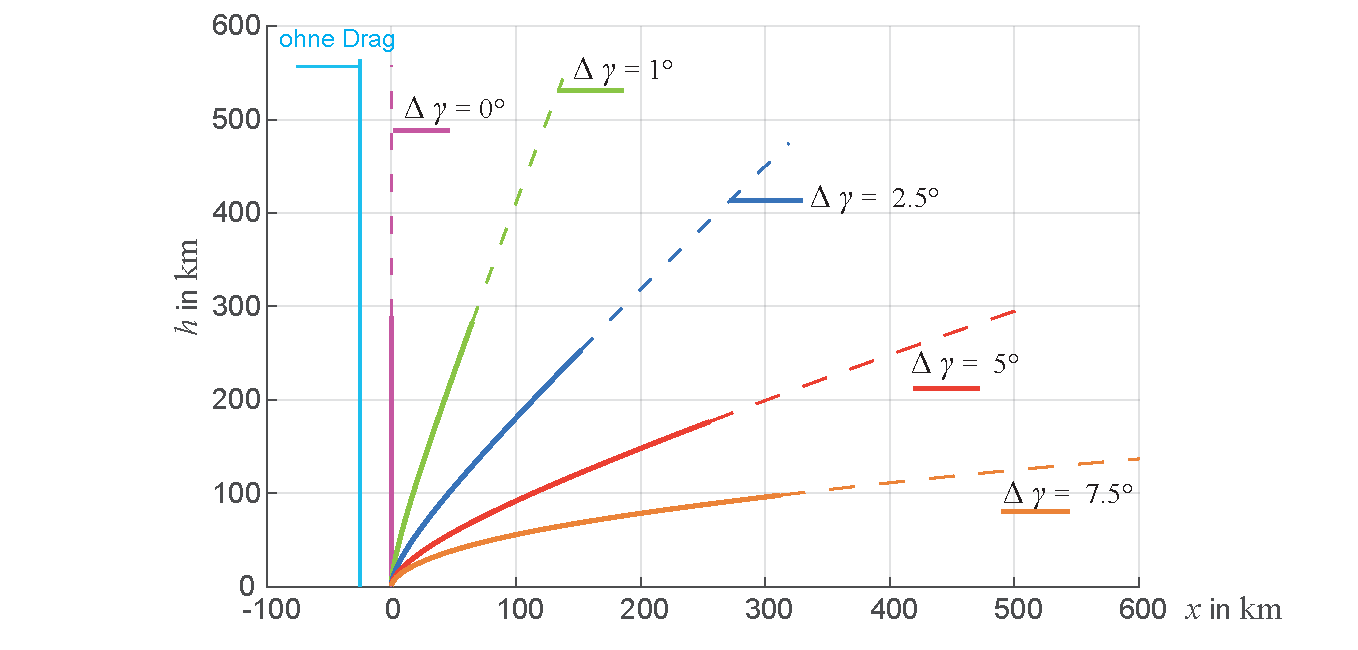
\includegraphics[width=\textwidth]{RaketenstartReal.pdf}
\caption[Trajektorie eines Raketenstarts von der Erdoberfl�che.]{Trajektorie eines Raketenstarts von der Erdoberfl�che f�r verschiedene Nickwinkel $\Delta \gamma$. Parameter: 
$c_\text{D}\,A = \SI{1.5}{\metre\squared}$ (Widerstandsbeiwert x Fl�che), $m_0 = \SI{1e5}{\kg}$ (Startmasse), $m_\text{L} = \SI{5e3}{\kg}$ (Payload), $\dot{m} = \SI{500}{\kg\per\second}$ (Masseverlust), $F_\text{S} = \SI{1.47e3}{\newton}$ (Schub), Nickkorrektur nach $t = \SI{20}{\second}$, Ende Schub nach $t_\text{BO} = \SI{190}{\second}$ (Brennschluss). F�r die Abh�ngigkeit der Dichte von der H�he wurde \eqref{eq:adyn_barom_h_fomulae} verwendet. Die Trajektorien bis zum Burn-Out sind durchgestrichen gezeichnet, f�r $t > t_\text{BO}$ gestrichen. Zum Vergleich ist die Trajektorie f�r eine Situation ohne Drag in Hellblau und der Startplatz um $\Delta x = \SI{-25}{\km}$ verschoben gezeigt. Siehe auch \mscr{} \mladynref{RaketenstartReal.m} f�r weitere Details und Graphiken.}
\label{abb:adyn_launch03}
\end{figure}

Die Endgeschwindigkeit $v_\text{f}$ im \KOS\ der Erde wird noch durch die von der Erde mitgegebene Anfangsgeschwindigkeit $\Delta v_\text{E,t}$ erh�ht (vorausgesetzt der Flug erfolgt in Richtung der Erdrotation und die Inklination der Bahn entspricht ungef�hr der geographischen Breite des Startplatzes). Dieser Beitrag ergibt sich zu:
\begin{align}
	 \Delta v_\text{E,t}& = \SI{0.465}{\km\per\second}\,\cos\phi_0\,.  \label{eq:adyn_launch10}
\end{align}
Hierin ist $\phi_0$ die geographische Breite des Startorts.\\
In \probref{adyn_launch01} wollen wir verschiedene Fragen des Raketenstarts genauer beleuchten. Wir werden den Einfluss der Erdrotation und des Richtungsvektors nach Start f�r verschieden geographische Breiten der jeweiligen Startorte ber�cksichtigen. Ebenso wollen wir den Start einer mehrstufigen Rakete mit den Werten aus Tabelle \ref{tab:adyn_parameter_raketen} simulieren. 

\subsection{Wiedereintritt eines Raumschiffs in die Erdatmosph�re}\label{kap:adyn_reentry}

Wie im vorherigen Kapitel bereits angemerkt, kann die Dynamik des Wiedereintritts in die Erdatmosph�re (\textit{Reentry}\index{Reentry}) durch die gleichen Bewegungsgleichungen  beschrieben werden, die wir f�r die Start- und Anfangsphase eines Raumfluges hergeleitet hatten (Gleichungen \eqref{eq:adyn_launch_vec} und \eqref{eq:adyn_launch01}). Allerdings sind die Anfangs- und Randbedingungen voneinander verschieden, was zu deutlich unterschiedlichen Effekten f�hrt (\figref{adyn_launch02}). Au�erdem ist im Fall des Wiedereintritts kein Schub zu ber�cksichtigen, daf�r ist aber \ia der beim Start/Aufstieg vernachl�ssigte Auftrieb durchaus von Bedeutung. Bevor wir uns mit der Dynamik des Wiedereintritts genauer besch�ftigen, wollen wir kurz auf die thermischen Problemstellungen eingehen, die mit dem Wiedereintritt in die Erdatmosph�re verbunden sind. 

\subsubsection{Thermodynamische �berlegungen zum Wiedereintritt}

Eine Raumsonde, die aus einem Erdorbit in einer H�he von \ca $\SI{125}{\km}$ wieder in die Erdatmosph�re eintritt, besitzt in etwa eine spezifische kinetische Energie von 
\begin{align*}
    T = \frac{1}{2}\,v_\text{k}{}^2 \approx \SI{31}{\mega\J\per\kg}\,.
\end{align*}
Diese Energie wird in der Phase des Wiedereintritts innerhalb typischer Zeiten $\tau \approx \SI{30}{}\ldots\SI{120}{\second}$  durch die atmosph�rische Bremsung in W�rmeenergie $Q_\text{th} = 
\dot{Q}_\text{th}\,\tau$ umgewandelt und muss dissipiert werden. Dabei werden interessanterweise $99.9\%$ der W�rmeleistung $P_\text{th}$ in die die Sonde umflie�ende Str�mung der atmosph�rischen Teilchen \anf{wegtransportiert}. Nur $0.1\%$ von $P_\text{th}$ \cite{Walter2018} m�ssen vom Raumschiff aufgenommen und auch wieder abgestrahlt werden. Nach dem Stefan\footnote{Josef Stefan (1835--1938) war ein �sterreichischer Mathematiker und Physiker, der auf den Gebieten der Akustik, Optik und der W�rmeleitung von Gasen sowie der Abh�ngigkeit der W�rmestrahlung von der Temperatur arbeitete.}\indexp{Stefan, Josef}-Boltzmann-Gesetz\index{Stefan-Boltzmann-Gesetz}\footnote{Ludwig Eduard Boltzmann (1844--1906) war ein �sterreichischer Physiker. Seine bedeutendsten Leistungen liegen im Bereich der Thermodynamik und der statistischen Mechanik. Er war einer der vehementesten Verfechter der Atomistik und gilt als einer der Vollender der klassischen Physik des 19. Jahrhunderts.}
%Schwer depressiv erkrankt auch auf Grund vieler Anfeindungen, nahm er sich im Alter von 62 Jahren das Leben.}
\indexp{Boltzmann, Ludwig Eduard} f�r einen schwarzen Strahler \cite{Meschede2010} ist die abgestrahlte Leistung eines solchen Strahlers mit seiner Temperatur �ber
\begin{align}
    T^4 = 0.001\,\frac{P_\text{th}}{\sigma\,A} \label{eq:adyn_reentry01}
\end{align}
verkn�pft, worin $\sigma$ die Stefan-Boltzmann-Konstante\index{Stefan-Boltzmann-Konstante} mit $\sigma = \SI{5.6705e-8}{\W\per\metre\squared\per\raiseto{4}\K}$ und $A$ die Fl�che des strahlenden K�rpers (\zb des Hitzeschildes der Sonde) sind. Setzen wir typische Werte von  $m=\SI{3000}{\kg}$, $A=\SI{3}{\square\metre}$, $\tau = \SI{30}{\second}$ ein, dann erhalten wir Temperaturen bis zu $T\approx\SI{1400}{\K}$. Dies gibt ein Gef�hl f�r die Temperaturen, die durch ein entsprechend konstruiertes Hitzeschild ausgehalten werden m�ssen. 

\subsubsection{Berechnung der Anfangsbedingung am �bergangspunkt} \label{kap:ady_reentry_conditions}

\figref{adyn_launch01}b und \figref{adyn_launch02}b zeigen den �bergangspunkt von der freien Trajektorie in die eigentliche Phase des aerodynamischen Wiedereintritts in die Atmosph�re. Man hat festgelegt, dass dieser Punkt einheitlich in einer H�he von $h_\text{Re} = \SI{400000}{}\,\mathrm{ft} \approx \SI{122}{\km}$ liegen soll (\figref{adyn_reentry02}).
Damit wird eine entsprechende Sph�re mit dem Radius $ h_\text{Re} = \SI{6500}{\km}$ definiert, bei welcher die Atmosph�re beginnt, einen signifikanten Einfluss auf das Raumschiff zu haben. Man berechnet die Dichte in $h_\text{Re}$ nach der barometrischen H�henformel\index{H�henformel!barometrisch} \eqref{eq:adyn_barom_h_fomulae} zu
\begin{align*}
    \varrho_\text{Re}= \varrho(h_\text{Re}) = \varrho_0\,\e^{-h_\text{Re}/H_0} = \SI{21.7}{\kg\per\km\cubed}\,. 
\end{align*}
Verbesserte Modelle der Atmosph�re wie CIRA-72 oder das Harris-Priester-Modell \cite{Vallado2007} liefern f�r $\varrho_\text{Re}$ Werte zwischen $\SI{24.49}{\kg\per\km\cubed}$ und $\SI{19,73}{\kg\per\km\cubed}$. Die einfache barometrische H�henformel ist also f�r uns eine brauchbare N�herungsformel. \\
Aus den Beziehungen f�r eine Kepler-Ellipse (\kap{hm_abl_kepler}) lassen sich folgende Beziehungen f�r die Gr��en am �bertrittspunkt gewinnen (\figref{adyn_launch01} mit $r_\text{Re} = R_\text{E} + h_\text{Re}$): 
\begin{subequations}
\begin{align}
    \cos\gamma_\text{Re} &= \frac{1+e\,\cos\upsilon_\text{Re}}{\sqrt{1+2e\,\cos\upsilon_\text{Re} +e^2}}\,,\label{eq:adyn_reentry02a}\\
    v_\text{Re} &= \frac{\mu_\text{E}}{L}\,\sqrt{1+2e\,\cos\upsilon_\text{Re}+e^2} \label{eq:adyn_reentry02b} \,,\\
    r_\text{e} &= \frac{a\,\lk 1-e^2\rk}{1+e\,\cos\upsilon_\text{Re}} = R_\text{E} +h_\text{Re}\,.\label{eq:adyn_reentry02c}
\end{align} \label{eq:adyn_reentry02}
\end{subequations}

\begin{figure}[H]
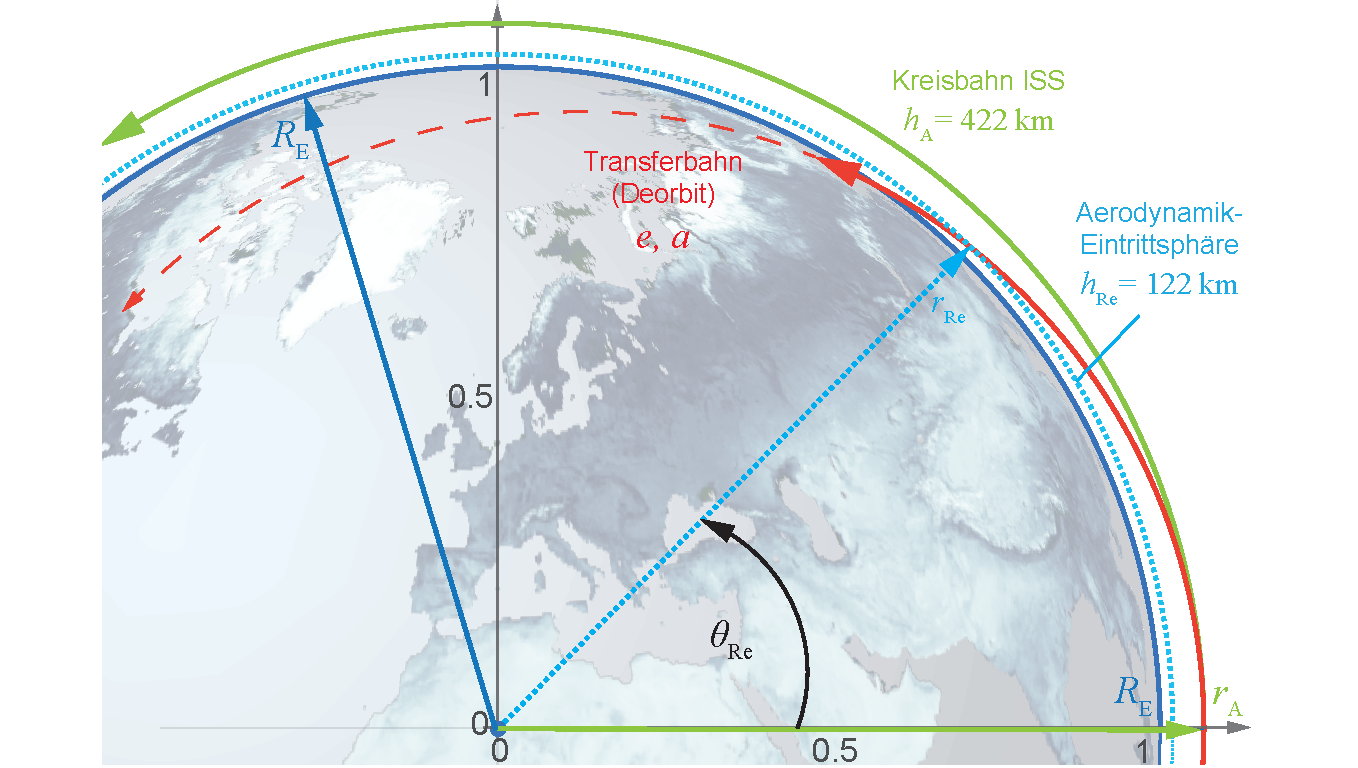
\includegraphics[width=0.8\textwidth]{ReentryGeometrie01.pdf}
\caption[Wiedereintritt-Transferbahn.]{Wiedereintritt-Transferbahn (Deorbit). Parameter: $r_\text{A} = R_\text{E} + \SI{422}{\km} =\SI{6800}{\km}$, $q=1.0462$.
Siehe auch \mscr{}\mladynref{Transfer2Reentry.m} f�r weitere Details und Graphiken.}
\label{abb:adyn_reentry02}
\end{figure}

Hier sind $\gamma_\text{Re}$ der FPA und $r_\text{Re}$ der Abstand zum Erdzentrum am �bergangspunkt bekannte Gr��en. Gesucht sind der Bahnparameter $e,\,a, \upsilon_\text{Re}$ der freien Trajektorie bis zum Wiedereintrittspunkt (im Englischen auch \textit{Deorbit}, also Abstiegsbahn genannt), die Geschwindigkeit $v_\text{Re}$ und der notwendigen Antriebsbedarf $\Delta v$ beim Apog�um $\Delta v$ (\figref{adyn_reentry01}). 
Der Drehimpuls der Bahn ist nach \eqref{eq:hm_drehimpuls_von_ae} gegeben durch:  $L=\sqrt{\mu_\text{E}\,a\,\lk 1-e^2\rk}$. Wir setzen  
\begin{align*}
    q=\frac{r_\text{A}}{r_\text{Re}} > 1\,.
\end{align*}
F�r die Berechnung des Wiedereintritts kann $q$ �ber $r_\text{A}$ als bekannt angenommen werden, ebenso wie der  FPA beim Eintritt $\gamma_\text{Re}$. Dieser wird aus Gr�nden der thermischen Belastung  \ia kleiner als $10\degree$ gew�hlt. Aus \eqref{eq:adyn_reentry02} findet man leicht:
\begin{subequations}
\begin{align}
    e &= \frac{q^2-\lk 2q-1\rk\,\cos^2\gamma_\text{Re}}{q^2-\cos^2\gamma_\text{Re}}\,, \\
    v_\text{Re} &= \sqrt{\frac{2\mu_\text{E}}{r_\text{A}}\,\frac{q^2\,(q-1)}{q^2-\cos^2\gamma_\text{Re}} }\,, \\
    \cos \upsilon_\text{Re} &= \frac{(q-1)^2\cos^2\gamma_\text{Re}- q^2\sin^2\gamma_\text{Re}}{(q-1)^2+(2\,q-1)\,\sin^2\gamma_\text{Re}}\,,\\
   \Delta v &= \frac{\mu_\text{E}}{r_\text{A}} - \cos\gamma_\text{Re}\,\frac{v_\text{Re}}{q}\,.
\end{align}\label{eq:adyn_reentry03}
\end{subequations}

\begin{figure}[H]
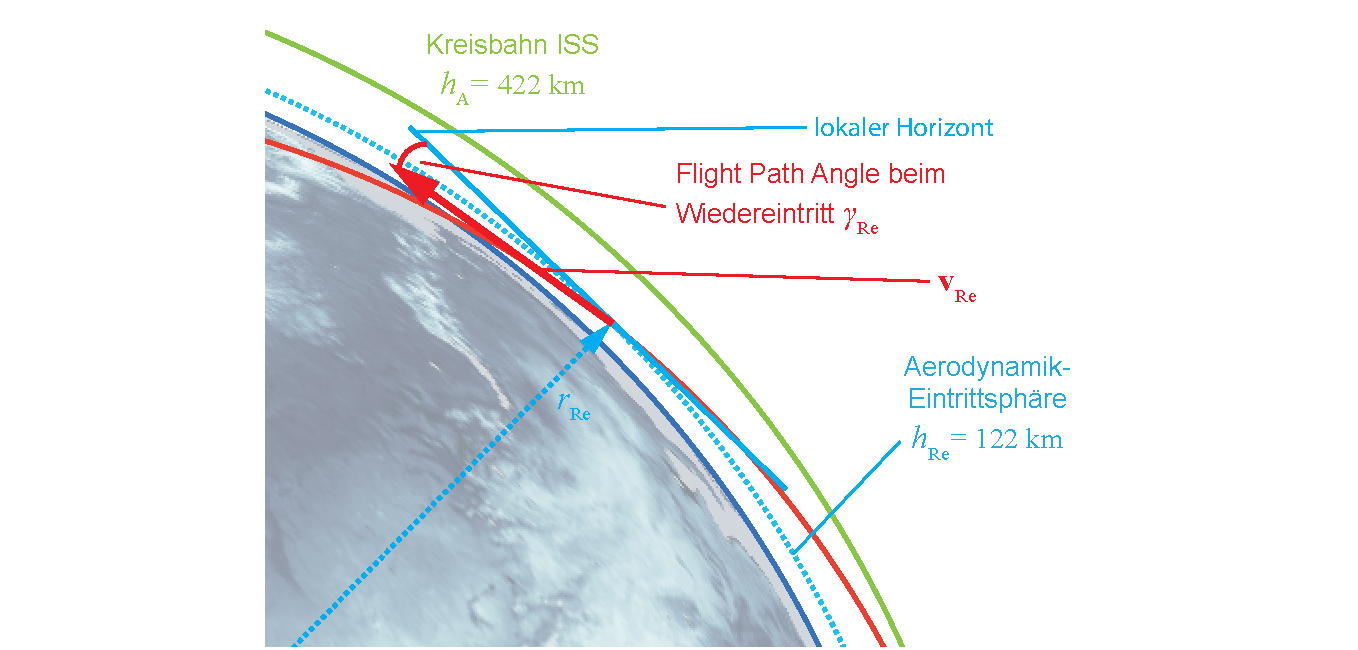
\includegraphics[width=0.95\textwidth]{ReentryGeometrie02.pdf}
\caption[Parameter zur Berechnung der Wiedereintritt-Transferbahn.]{Parameter zur Berechnung der Wiedereintritt-Transferbahn (Deorbit). Die Festlegung von $h_\text{Re}$ auf eine nichtmetrische SI-Einheit $\SI{400000}{}\,\mathrm{ft}$ kommt noch aus der Zeit, da die westliche Raumfahrtwissenschaft sehr stark durch die USA dominiert war. Es sind im �brigen schon Raumfahrtmissionen wegen unterschiedlicher Verwendung nichtmetrischer \bzw imperialer Einheiten und inkorrekter Konversion fehlgeschlagen. Das soll uns nicht passieren, weswegen wir ausschlie�lich das SI-Einheiten-System (siehe die \onlineZ) verwenden.}
\label{abb:adyn_reentry01}
\end{figure}

Wir �berlassen es dem Leser als �bung, die einzelnen Schritte zur Herleitung der Beziehungen \eqref{eq:adyn_reentry02} und \eqref{eq:adyn_reentry03} mit den Kenntnissen aus der Himmelsmechanik \kap{lsg_kepler} nachzuvollziehen (\probref{adyn_reentry01}). \\
Man berechnet nun nach \eqref{eq:adyn_reentry03} schrittweise $e$, $v_\text{Re}$ schlie�lich $\Delta v$ und $\upsilon_\text{Re}$ \bzw $\upsilon_\text{Re}$ =  $\left| \upsilon_\text{Re}- 180\degree \right|$.\\
%F�r diesen Fall und $q= \frac{r_\text{A}}{r_\text{Re}} \to 1$ kann man aus \eqref{eq:adyn_reentry03} eine N�herung erhalten:
%\begin{subequations}
%\begin{align}
    %\upsilon_\text{Re} &= \sqrt{\frac{\mu_\text{E}}{r_\text{A}}} \,\lk 1+\frac{3}{4}\,\lk q-1\rk -\frac{\gamma_\text{Re}{}^2}{8\,\lk q-1\rk}\rk\,,\\
    %\Delta v &= \sqrt{\frac{\mu_\text{E}}{A_\text{A}}}\,\lk q-1 + \frac{\gamma_\text{Re}{}^2}{2\,\lk q-1\rk}\rk
%\end{align}\label{eq:adyn_reentry04}
%\end{subequations}
Als Beispiel sei die R�ckkehr eines Transport-Raumschiffes von der ISS genannt. Man w�hlt einen FPA von $\gamma_\text{Re}=6\degree$ und erh�lt mit $r_\text{A} = R_\text{E} + \SI{422}{\km} =\SI{6800}{\km}$, $q=1.0462$ (siehe \mscr \mladynref{Transfer2Reentry.m} \figref{adyn_reentry02}): 
\begin{align*}
    \theta_\text{Re} = 45.5\degree\,, && v_\text{Re} =  \SI{7.50}{\km\per\second}\,, && \Delta v = -\SI{530}{\metre\per\second}\,.
\end{align*}
Wir k�nnen leicht numerisch oder auch analytisch aus \eqref{eq:adyn_reentry03} ableiten, dass f�r den Wiedereintritt aus einem LEO n�herungsweise gilt:
	\[ q \to 1\,, ~~v_\text{Re} \approx v_\text{K} =\sqrt{\frac{\mu_\text{E}}{R_\text{E}}} = \SI{7.905}{\km\per\second} ~~\text{(1.\,\gls{vkosmos})}\,. \]
Ebenso kann man sich �berlegen, dass f�r einen direkten Wiedereintritt in die Erdatmosph�re aus dem interplanetaren Raum die Anfangsbedingungen lauten: 
	\[ q \to \infty\,,~~ v_\text{Re} \approx \sqrt{\frac{2\mu}{r_\text{Re}}} = \SI{11.8}{\km\per\second} ~~\text{(2.\,\gls{vkosmos})}\,,\\
    ~~~~\upsilon_\text{Re} = 2\,\gamma_\text{Re}\,.\]

\subsubsection{Berechnung der Dynamik des Wiedereintritts in die Erdatmosph�re}

Wir l�sen nun mit den berechneten Anfangsbedingungen die Bewegungsgleichungen f�r die Wiedereintritt-Phase numerisch. Das Ergebnis ist in \figref{adyn_reentry03} und \figref{adyn_reentry04} gezeigt. In der ersten Abbildung ist der "`Gleitpfad"' $h(x)$ f�r zwei verschiedene initiale FPA $\gamma_\text{Re}$ gezeigt. Erwartungsgem�� wird bei einem steilen Eintauchen in die Erdatmosph�re $\gamma_\text{Re} \approx 10\degree$ der Gleitpfad steiler und k�rzer und damit auch die thermische Belastung gr��er. 

\begin{figure}[H]
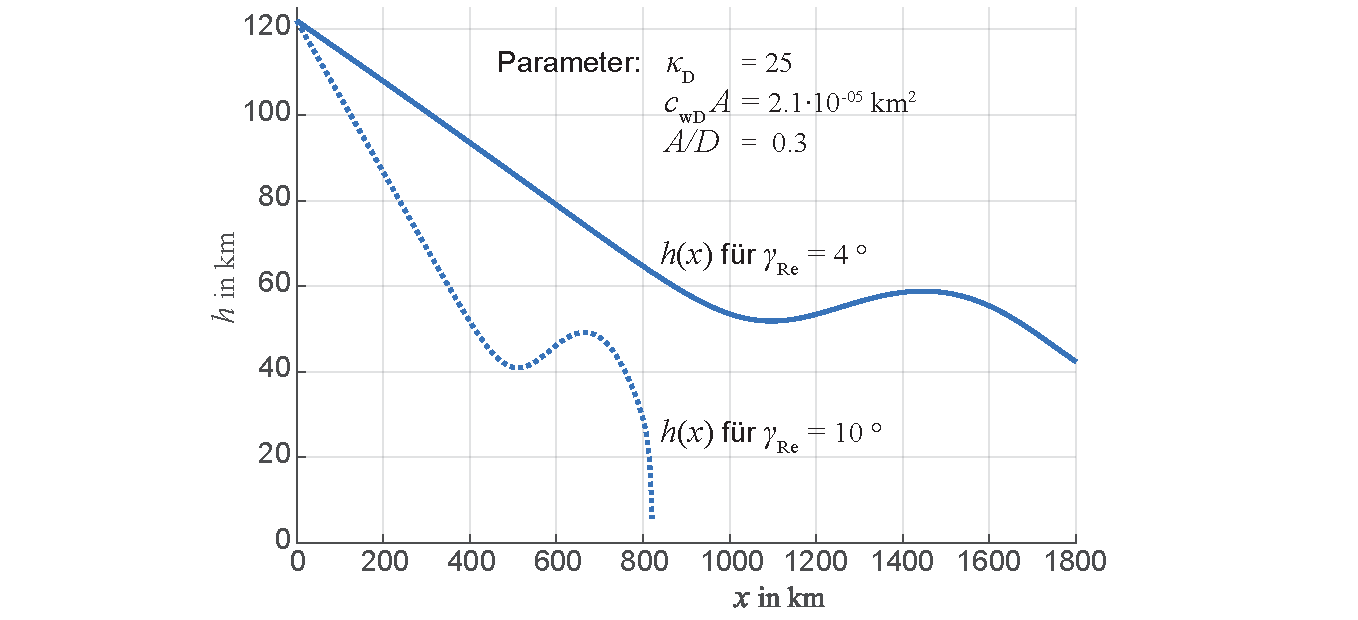
\includegraphics[width=\textwidth]{RaumschiffReentry01.pdf}
\caption[Gleitpfad beim Wiedereintritt.]{Gleitpfad beim Wiedereintritt f�r zwei verschiedene initiale FPA $\gamma_\text{Re}$. Parameter:
$c_\text{D}\cdot A = \SI{1.5}{\metre\squared}$ (Widerstandsbeiwert $\cdot$ Fl�che), $m_\text{L} = \SI{5e3}{\kg}$ (Payload). F�r die Abh�ngigkeit der Dichte von der H�he wurde \eqref{eq:adyn_barom_h_fomulae} verwendet. Siehe auch \mscr{} \mladynref{ReentrySummary.m} f�r weitere Details und Graphiken.}
\label{abb:adyn_reentry03}
\end{figure}

In \figref{adyn_reentry04} sind neben dem H�henverlauf $h(t)$ auch der Geschwindigkeitsverlauf $v(t)$ und die Beschleunigung (Abbremsung) $a(t)$  �ber der Zeit aufgetragen. Deutlich zu erkennen sind die einzelnen Phasen des Abbremsens, so bei $t=50 \ldots 90\,\mathrm{s}$ f�r $\gamma_\text{Re} = 10\degree$ \bzw $t= 100 \ldots 180\,\mathrm{s}$ f�r $\gamma_\text{Re} = 4\degree$. Im zweiten Fall ist also die thermische Belastung (Temperaturerh�hung) auf Grund der doppelt so langen "`Bremszeit"' auf etwa 85\% und die gegebenenfalls durch Astronauten auszuhaltende Maximalbeschleunigung von $20\,g$ auf etwa $5\,g$ reduziert.
\begin{figure}[H]
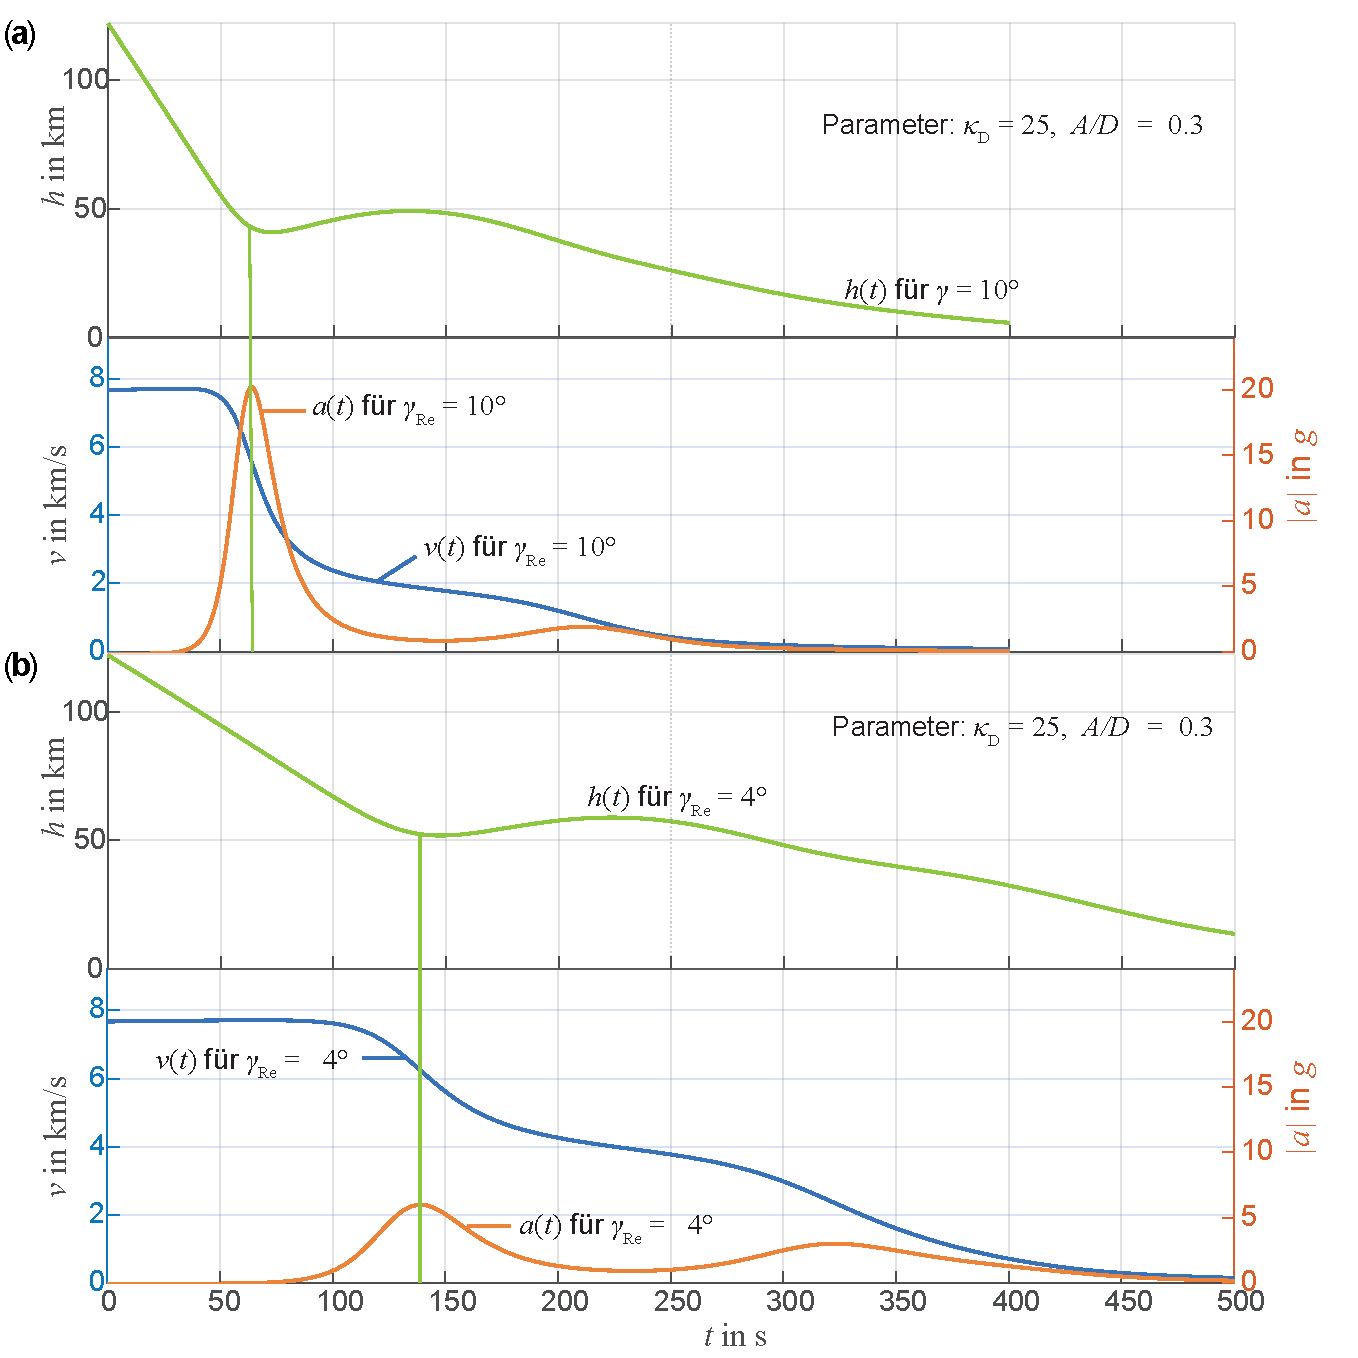
\includegraphics[width=1.0\textwidth]{RaumschiffReentry02.pdf}
\caption[Zeitverl�ufe beim Wiedereintritt.]{Zeitverl�ufe beim Wiedereintritt f�r $h,\, v$ und $a$. Parameter: 
$c_\text{D}\cdot A = \SI{1.5}{\metre\squared}$ (Widerstandsbeiwert $\cdot$ Fl�che), $m_\text{L} = \SI{5e3}{\kg}$ (Payload). F�r die Abh�ngigkeit der Dichte von der H�he wurde \eqref{eq:adyn_barom_h_fomulae} verwendet. \fa initialer FPA $\gamma\text{Re} = 10\degree$,  \fb initialer FPA $\gamma\text{Re} = 4\degree$. Siehe auch \mscr{} \mladynref{ReentrySummary.m} f�r weitere Details und Graphiken.}
\label{abb:adyn_reentry04}
\end{figure}

Ebenso erkennbar sind Phasen ann�hernd konstanter Geschwindigkeit und Phasen in denen es auf Grund eines speziellen Auftrieb/Drag-Verh�ltnisses sogar kurzzeitig zu einem Ansteigen des Raumschiffs kommen kann. Diese Abh�ngigkeit untersuchen wir in \probref{adyn_reentry02}.

\subsubsection{N�herungsformel f�r einzelne Phasen}

Wir wollen nun noch f�r einzelne Phasen des Wiedereintritts einfache N�herungsbeziehungen herleiten. Dabei wenden wir eine h�ufig benutzte Methode an, mit der das noch recht komplexe Differentialgleichungssystem \eqref{eq:adyn_launch08}, in welchem wir wieder den Auftrieb ber�cksichtigen wollen, weiter vereinfacht werden kann. F�r den Drag und den Auftrieb benutzen wir wiederum die barometrische H�henformel 
\begin{align}
    F_\text{D} &= m_\text{R}\,v^2 \frac{\kappa_\text{D}}{H_0} \e^{-h/H_0} ~~~\text{\bzw}~~~
    F_\text{A} = m_\text{R}\,v^2 \frac{\kappa_\text{A}}{H_0} \e^{-h/H_0} \,. \label{eq:adyn_reentry10a}
\end{align}
F�r das Verh�ltnis von Auftrieb zu Drag schreiben wir $A/D = \kappa_\text{A}/\kappa_\text{D}$.
Die Gleichung \eqref{eq:adyn_launch08c} kann benutzt werden um �ber $t=t\lk h\rk$ die Zeitvariable zu eliminieren, womit wir $v\lk h\rk$ und $\gamma\lk h\rk$ bekommen. Gleichzeitig wollen wir zu dimensionslosen Gr��en �bergehen. F�r die Geschwindigkeit schreiben wir $\mu = v/v_\text{K}$ mit $v_\text{k} = \sqrt{\mu_\text{E}/R_\text{E}}$ als die 1.~\gls{vkosmos}. F�r die H�he und Bodendistanz $\eta=h/H_0$ \bzw $\xi=x/H_0$ und f�r die Zeit $\tau= t\,g_\text{E}/v_\text{K}$, worin $g_\text{E}= \mu_\text{E}/R_\text{E}{}^2$ die Erdbeschleunigung auf der Erdoberfl�che ist.
Zum Schluss f�hren wir noch eine dimensionslose spezifische kinetische Energie $\hat{\epsilon}$ ein:
\begin{align}
    \hat{\epsilon} = \mu^2 = \frac{v^2}{v_\text{K}{}^2}~.\label{eq:adyn_reentry10b}
\end{align}
Die dimensionslose H�he $\eta=h/H_0$ skalieren wir exponentiell entsprechend der barometrischen H�henformel zur ebenfalls diemensionslosen H�he $\hat{\eta}$:
\begin{align}
    \hat{\eta} = \frac{2\,\kappa_\text{D}}{\sin\gamma_\text{Re}}\,\e^{-\eta} \;.\label{eq:adyn_reentry10c}
\end{align}
Nach etwas Algebra, die wir in \probref{adyn_reentry03} ausgef�hrt haben, erhalten wir aus \eqref{eq:adyn_launch08}:
\begin{subequations}
\begin{align}
    \frac{\D \lk \ln\hat{\epsilon}\rk}{\D\hat{\eta}} &= -\underbrace{\frac{\sin\gamma_\text{Re}}{\sin\gamma}}_{\text{Drag}}\, + \underbrace{\frac{2H_0}{\hat{\epsilon}\,\hat{\eta}\,R_\text{E}}}_{\text{Gravitation}}\,, \label{eq:adyn_reentry11a}\\
    \frac{\D \lk\cos\gamma\rk}{\D \hat{\eta}} &= \underbrace{\frac{\sin\gamma_\text{Re}}{2}\,\frac{A}{D}}_{\text{Auftrieb}} \,- \underbrace{\lk\frac{1}{\hat{\epsilon}-1}\rk\,\frac{H_0\,\cos\gamma}{\hat{\eta}\,R_\text{E}}}_{\text{Gravitation, Zentrifugalkraft}} \,.\label{eq:adyn_reentry11b}
\end{align} \label{eq:adyn_reentry11}
\end{subequations}

Wir haben zwei Gleichungen erhalten. Die erste beschreibt die Ver�nderung der (dimensionslosen) Energie �ber die dimensionslose H�he und die zweite die Ver�nderung des FPA ebenfalls �ber die dimensionslose H�he.  Auf den ersten Blick sieht das nicht wie ein Fortschritt aus, aber die Gleichungen zeigen eine Separation in vier Terme, die den wirkenden Kr�ften (Auftrieb, Drag, Gravitation und Zentrifugalkraft) zugeordnet werden k�nnen. Aus
\begin{align*}
    a = \frac{\D v}{\D t}= \frac{\D v}{\D \lk\ln\hat{\epsilon}\rk}\,\frac{\D\lk\ln\hat{\epsilon}\rk}{\D\hat{\eta}}\,\frac{\D\hat{\eta}}{\D h}\,\frac{\D h}{\D t}
\end{align*}
folgt
\begin{align}
    a &= \frac{\hat{\epsilon}\,v_\text{K}{}^2}{2v} \,\lek - \frac{\sin\gamma_\text{Re}}{\sin\gamma} + \frac{2H_0}{\hat{\epsilon}\,\hat{\eta}\,R_\text{Re}}\rek\,\lk -\frac{\hat{\eta}}{H_0}\rk\,\lk-v\,\sin\gamma\rk \nonumber \\
    \rightarrow~~~a &= -g_\text{E}\,\lk \frac{\hat{\epsilon}\,\hat{\eta} \,R_\text{E}}{2H_0}\,\sin\gamma_\text{Re} - \sin\gamma\rk\,. \label{eq:adyn_reentry12}
\end{align}
Damit haben wir eine Gleichung gewonnen, die uns erlaubt, abh�ngig von den Parametern $H_0$, $\kappa_\text{D}$, $A/D$ und $\gamma_\text{Re}$ eine Absch�tzung f�r die Beschleunigung zu machen. Wir wollen das an zwei Phasen verdeutlichen:
\subparagraph{Phase ohne Drag}
Wir k�nnen $\kappa_\text{D}\approx 0$ setzen und erhalten aus \eqref{eq:adyn_reentry12}:
\begin{subequations}
\begin{align}
    a &= \dot{v} = g_\text{E}\,\sin\gamma \,,\\
    \dot{\gamma} &= 0\,,\\
    \dot{h} &= -v\,\sin\gamma
\end{align} \label{eq:adyn_reentry13}
\end{subequations}
mit den einfachen L�sungen 
\begin{subequations}
\begin{align}
    \gamma &= \gamma_\text{Re} \,,\\
    h &= h_\text{Re} - v_\text{Re}\,\sin\gamma_\text{Re}\,t \,,\\
    v &= v_\text{Re} + g_\text{E}\,\sin\gamma_\text{Re}\,t\approx v_\text{Re}\,.
\end{align}\label{eq:adyn_reentry14}
\end{subequations}

\begin{figure}[H]
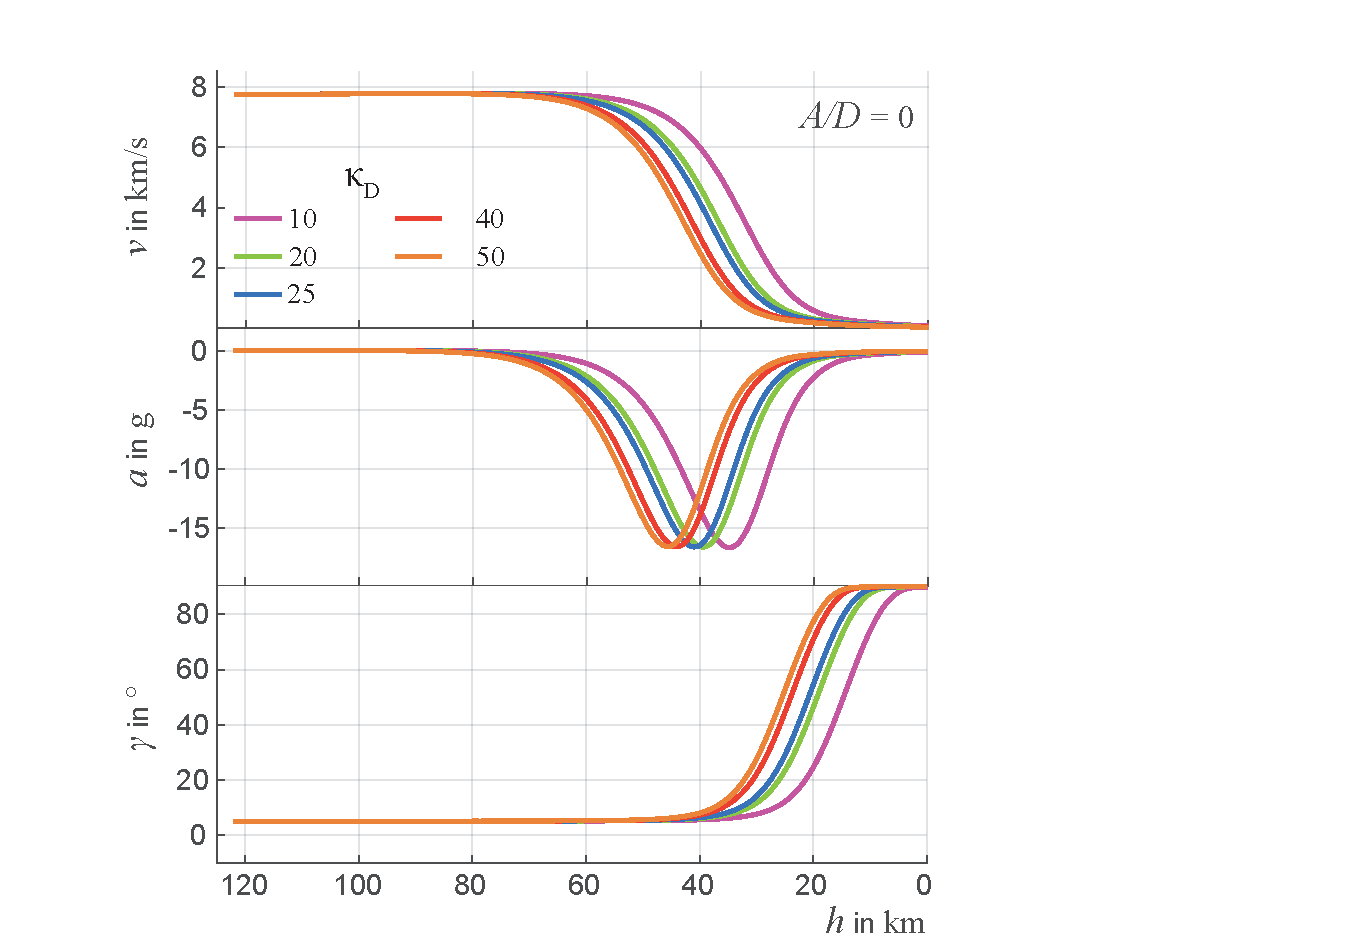
\includegraphics[width=\textwidth]{ReentryNaeherungen01.pdf}
\caption[L�sungen der Bewegungsgleichungen f�r den Wiedereintritt.]{L�sungen der Bewegungsgleichungen f�r den Wiedereintritt f�r verschiedene Reibungskoeffizienten. Siehe auch \mscr{} \mladynref{ReentryNaeherungen.m} f�r weitere Details und Graphiken.}
\label{abb:adyn_reentry05}
\end{figure}

Wir k�nnen das sehr gut in \figref{adyn_reentry05} und \figref{adyn_reentry06} erkennen. Wann aber ist nun das Ende dieser Phase erreicht?
Dazu betrachten wir \eqref{eq:adyn_reentry11a} und sehen, dass $\D \ln\hat{\epsilon} / \D \hat{\eta}< 0$ wird, wenn
\begin{align}
    \frac{\sin\gamma_\text{Re}}{\sin\gamma} = \frac{2H}{\hat{\epsilon}\,\hat{\eta}\,R_\text{E}}\label{eq:adyn_reentry15}\,.
\end{align}
In der initialen Phase ist aber $\hat{\epsilon}\approx 1$ und $\gamma\approx \gamma_\text{Re}$, so dass daraus eine Bedingung f�r $h$ entsteht, bei welcher die sogenannte ballistische Phase beginnt:
\begin{align}
    \hat{\eta} &= \frac{2H_0}{R_\text{E}} ~~ \to ~~ \frac{2\,\kappa_\text{D}}{\sin\gamma_\text{Re}}\,\e^{-\frac{h}{H_0}} = \frac{2H_0}{R_\text{E}} ~~\to ~~ h = -H_0\,\ln\,\frac{H_0\,\sin\gamma_\text{E}}{R_\text{E}\,\kappa_\text{D}}\,.\label{eq:adyn_reentry16}
\end{align}
Wegen $\D \hat{\epsilon} /\D \hat{\eta} = 0 $ ist das auch die H�he, bei der die maximale Geschwindigkeit erreicht wird.

\begin{figure}[H]
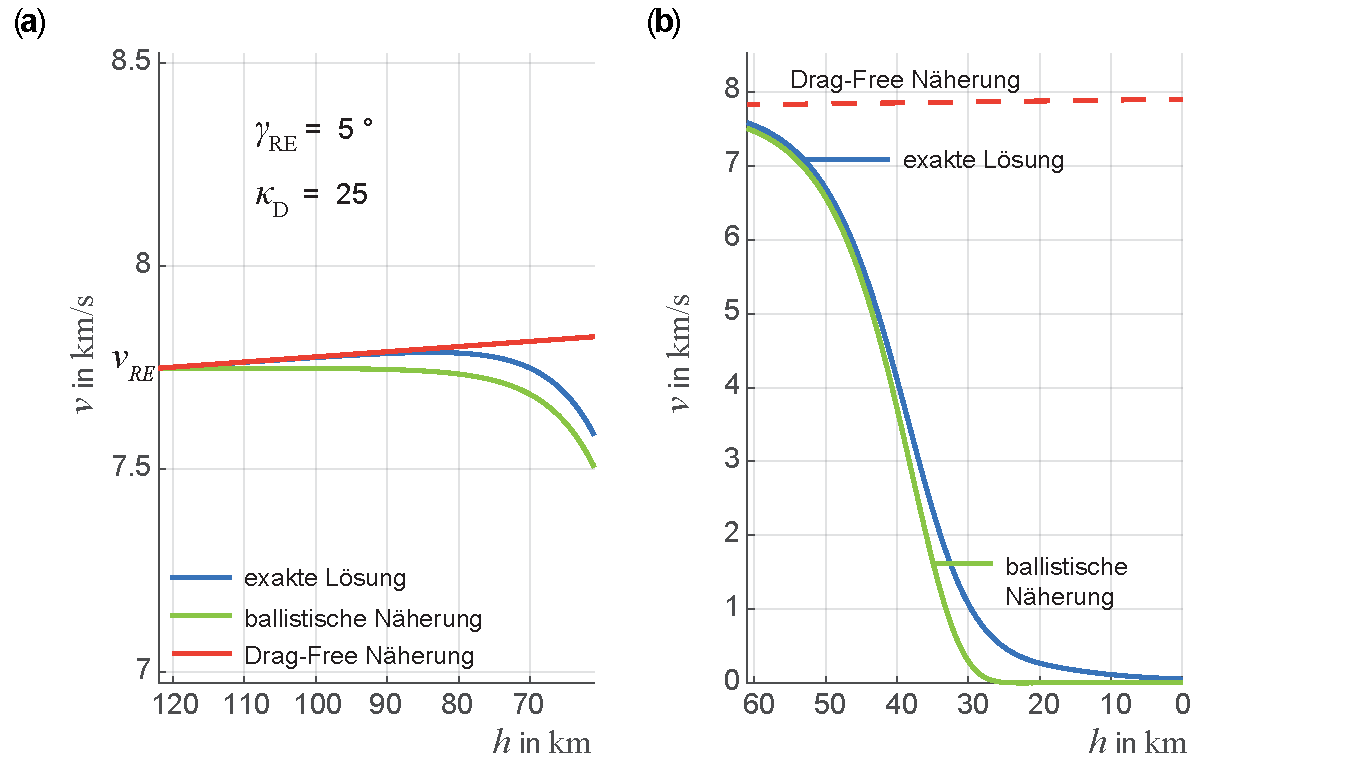
\includegraphics[width=\textwidth]{ReentryNaeherungen02.pdf}
\caption[N�herungsl�sungen normierte Bewegungsgleichungen f�r Wiedereintritt.]{N�herungsl�sungen der normierten Bewegungsgleichungen f�r den Wiedereintritt im Vergleich zur "`exakten"' L�sung. \fa Free-Drag Phase \fb Ballistische Phase. Man erkennt, dass fast unabh�ngig von $\kappa_\text{D}$ die Abbremsung auf eine gleichf�rmige Bewegung in einer H�he von ca. 40 km erfolgt. Siehe auch \mscr{} \mladynref{ReentryNaeherungen.m} f�r weitere Details und Graphiken.}
\label{abb:adyn_reentry06}
\end{figure}

\subparagraph{Ballistische Phase mit gro�em Drag}
Die nachfolgende Phase soll unter der Vereinfachung betrachtet werden, dass alle anderen Kr�fte au�er dem Drag vernachl�ssigt werden k�nnen, \dh $A=0$, $\hat{\epsilon}\approx 1$. 
Dann folgt aus \eqref{eq:adyn_reentry11}:
\begin{align}
\begin{split}
    \frac{\D \ln\hat{\epsilon}}{\D \hat{\eta}} &= -\frac{\sin\gamma_\text{Re}}{\sin\gamma} + \underbrace{\frac{2H_0\,\sin\gamma_\text{Re}}{R_\text{E}\,\kappa_\text{D}}\,\e^{\frac{h}{H_0}}}_{\approx 0}\,,\\
    \frac{\D \cos\gamma}{\D \hat{\eta}} &= 0 \,\,. 
\end{split}   \label{eq:adyn_reentry17}
\end{align}
Das System l�sst sich leicht l�sen und wir erhalten mit $\gamma = \gamma_\text{Re} = \con $ und 
\begin{align}
    \ln\,\frac{\hat{\epsilon}}{\hat{\epsilon}_\text{Re}} &= -\lk\hat{\eta}-\hat{\eta}_\text{Re}\rk \to ~~~ \hat{\epsilon} = \hat{\epsilon}_\text{Re}\,\e^{-\hat{\eta}_0-\hat{\eta}_\text{Re}}\approx\hat{\epsilon}_\text{Re}\,\e^{-\hat{\eta}}\,,\nonumber\\
    v &\approx v_\text{Re}\,\e^{-\frac{\hat{\eta}}{2}} = v_\text{Re}\,\e^{-\lek\frac{\kappa_\text{D}}{\sin\gamma_\text{Re}}\,\e^{-h/H_0}\rek}\,.\label{eq:adyn_reentry18}
\end{align}
Auch diese Phase ist in \figref{adyn_reentry06} gut zu erkennen. \\

Wir m�chten zum Schluss noch einmal darauf hinweisen, dass neben dem Drag auch das nichtsph�rische Gravitationsfeld der Erde und der Strahlungsdruck einen abbremsenden Charakter auf Raumsonden in niedrigen Orbits haben. In \probref{adyn_reentry04} werden wir ein sehr einfaches Modell einer solchen abfallenden, sinkenden Umlaufbahn untersuchen.
Wir konnten mit diesem kurzen Exkurs das hochinteressante Thema des Wiedereintritts von Raumschiffen in die Erdatmosph�re nur anrei�en und m�ssen den interessierten Leser f�r weitere Details an die entsprechende Fachliteratur verweisen \cite{Walter2018, Veris2018}, womit wir dann auch das sch�ne Kapitel der Astrodynamik schlie�en. \\
 
%\clearpage
%%%% Anmerkung 2023-11-13 (mk.):
%%% Links auf L�sungen komplett auskommentiert, da extra file bew_uebungenAB.tex
%%% Einfaches �ndern durch  ersetzen \hyperref.. <--> %\hyperref.

%%% Links basieren f�r ein m�gliches e_book auf getrennter pdf-Zieldokumente auf pdf-Hypertags:
%%%        \linklsg\\%\href{FingerUeb2_AB.pdf#prb:adyn_canonball}{\textcolor{blue} {$\rightarrow$ zur \probref{adyn_canonball}.}}\\
%%% Einfaches �ndern durch  ersetzen %href{FingerUeb1_AB.pdf.. <--> \linklsg\\%\href{FingerUeb1_AB.pdf..
%%%
%%% oder 
%%% f�r das Arbeitsbuch als geschlossenes Zieldokument auf normalen Verweisen (siehe bew_uebungenAB.tex):
%%%        \textcolor{blue} {$\rightarrow$ zur} \probref{adyn_canonball}.\\
%%%

\section{�bungen zu \autoref{chap:adyn} -- Astrodynamik}\label{kap:adyn_uebungen}

\medskip
Die �bungen sind mit Schwierigkeitsindikatoren markiert, von einfach ($\ast$) �ber mittel ($\ast \ast$) bis schwierig ($\ast \ast \ast$).
Zusatzaufgaben sind zum Teil mit ($\ast \ast \ast \;!$) markiert und eher als Erweiterung des Theorieteils zu betrachten.
Einige wenige �bungen sind rein analytisch, die gro�e Mehrzahl beinhaltet aber \matlab-Anwendungen. \\

L�sungsbeispiele finden sich in den \onlineZ{} im Arbeitsbuch {\textcolor{blue}{FingerUeb2\_AB.pdf}} und k�nnen �ber den Link \linklsg erreicht werden.\\
Die entsprechenden \mscre finden sich im GitHub unter \githubSN \bzw
in den \onlineZ{} (\MKc).\\

%%%-----------------------------------------------------------------------------------------------------------

\subsection{�bungen zu Grundlagen der Raketenphysik}

\medskip

%-----------------------------------------------------------------------------------------------------------

\begin{prob} %�bung1
\einfach{adyn_canonball}{Jules Vernes Kanonenschuss zum Mond}
In seinem Buch "`Von der Erde zum Mond"' berichtet Jules Verne, dass ein Kanonenclub in den USA einen Vorschlag machte, mit einer Kanone ein Geschoss von der Erde zum Mond zu schicken. Man plante eine Granate mit einer Nutzlast von $\SI{8.75}{\tonne}$ und einigte sich auf ein Gesch�tzrohr von $\SI{270}{\metre}$ L�nge aus Gusseisen. Als Treibladung sollte Schie�baumwolle (Zellulosenitrat) verwendet werden. %Als geeigneter Standort f�r die Kanone wurde der Bundesstaat Florida gew�hlt.\\
%Jules Vernes Astronauten starteten also genau so wie die sp�teren NASA-Astronauten in Florida und erneuerten den notwendigen Sauerstoff im Projektil durch Erhitzen von Kaliumchlorat.
Diskutieren Sie die Chancen, die drei Astronauten und zwei Hunde mit dieser Technik sicher zum Mond zu bringen.

\medskip
\linklsg\\%\href{FingerUeb2_AB.pdf#lsg:adyn_canonball}{\textcolor{blue} {$\rightarrow$ L�sungsteil}}.\\
%\hyperref[lsg:adyn_canonball]{\textcolor{blue} {$\rightarrow$ L�sungsvorschlag}}.\\
\noindent\rule[1ex]{\textwidth}{0.5pt}
\end{prob}

%-----------------------------------------------------------------------------------------------------------

\begin{prob} %�bung2
\einfach{adyn_rocketbasic}{Prinzip Mehrstufenrakete}
Man kann einige grunds�tzliche Erkenntnisse aus der Raketen-Gleichung \eqref{eq:adyn_rockets19} ableiten, wenn man \zb den Spezialfall gleicher Stufenmassen und gleicher Massen f�r alle $N$~Raketenstufen betrachtet, also $v_{\text{G},i} = v_\text{G}^*\,,~~ m_{0,i}/(m_{0,i}-m_{\text{T},i}) = \mathcal{M}^*\,$. Man erh�lt aus \eqref{eq:adyn_rockets19}:
\begin{align}
\begin{split}
     \Delta v_\text{ges} &=  N\,v_\text{G}^*\,\ln \mathcal{M}^* ~~\rightarrow ~~  \lk \mathcal{M}^* \rk^N = \e^{\Delta v_\text{ges}/v_\text{G}^*} ~~\text{\bzw} ~~ \mu_\text{L} =  \frac{m_\text{L}}{m_0} = \lk \mathcal{M}^* \rk^{-N}\,,
\end{split}  \label{eq:adyn_rockets20}
\end{align}
was bedeutet, dass das Antriebsverm�gen linear mit der Stufenzahl $N$ zunimmt, w�hrend das Nutzlastverh�ltnis exponentiell mit $N$ f�r diesen speziellen Fall der Massenverh�ltnisse abnimmt. Leiten Sie \eqref{eq:adyn_rockets20} her.

\medskip
%\hyperref[lsg:adyn_rocketbasic]{\textcolor{blue} {$\rightarrow$ L�sungsvorschlag}}.\\
\linklsg\\%\href{FingerUeb2_AB.pdf#lsg:adyn_rocketbasic}{\textcolor{blue} {$\rightarrow$ L�sungsteil}}.\\
\noindent\rule[1ex]{\textwidth}{0.5pt}
\end{prob}

%-----------------------------------------------------------------------------------------------------------

\begin{prob}  %�bung3
\schwierig{adyn_rocketopt1}{Optimierung Mehrstufenrakete (Tandemstufung)}
\begin{enumerate}
	\item \textit{\textbf{\anf{Optimieren} Sie Parameter der dreistufigen Saturn V Rakete mit 100 t Nutzlast �ber die Methode der Extremwertberechnung}}\\
          Nehmen Sie die Ausstr�mgeschwindigkeiten $v_{\text{G},i}$, die Strukturkoeffizienten $\sigma_i$ und die zu transportierende Nutzlast $m_\text{L}$ \bzw das Nutzlastverh�ltnis $\mu_\text{L}$ als gegeben an. Daten finden Sie dazu in Tabelle \ref{tab:adyn_parameter_raketen} im Tabellenanhang \kap{adyn_tabellen}. 
Formulieren Sie das Problem als Extremwertberechnung f�r $\Delta v_\text{g}$ in Abh�ngigkeit von den Massenverh�ltnissen $\mu_i$.\\

	\item \textit{\textbf{Berechnen Sie das erzielbare Nutzlastverh�ltnis der Saturn V Rakete f�r den Flug zum Mond �ber die Methode der der Lagrange-Multiplikatoren}}\\ 
Gehen von einem Antriebsbedarf $\Delta v_\text{g}= \SI{12.4}{\kilo\metre\per\second}$ aus. Vergleichen Sie Ihr Ergebnis mit dem tats�chlich von der NASA realisierten Nutzlastverh�ltnis.
F�r die Apollo 11 Mission w�hlte die NASA folgende Konfiguration der Saturn V Rakete (siehe Tab. \ref{tab:adyn_parameter_Apollo11}), um eine Nutzlast von $\SI{47000}{\kg}$ zum Mond zu bringen:
\begin{table}%tab1
\caption[Saturn V Konfiguration f�r die Apollo 11 Mission.]{Saturn V Konfiguration f�r die Apollo 11 Mission \cite{Walter2018}.}
\smallskip
\hspace{1.5cm}
\begin{tabular}{L{1.5cm}R{2cm}R{2cm}R{2cm}R{1.5cm}}
\svhline\noalign{\smallskip}
Gr��e				    			& 1. Stufe				& 2. Stufe   	    & 3. Stufe  		& Einheit \\
\noalign{\smallskip}\svhline\noalign{\smallskip}
\noalign{\smallskip}
$m_{0,i}$							&	$\SI{2902000}{}$	&	$\SI{ 658000}{}$	&	$\SI{  165000}{}$	&	$\SI{}{\kg}$	 \\	
$v_{\text{G},i}$			&	$\SI{  2980}{}$	&	$\SI{   4130}{}$	&	$\SI{    4130}{}$	&	$\SI{}{\metre\per\second}$	 \\	
$\sigma_i$						&	$\SI{0.0765}{}$	&	$\SI{0.1140}{}$	&	$\SI{0.1110}{}$	&	$\SI{}{}$	 \\	
\noalign{\smallskip}
\svhline\noalign{\smallskip}
\end{tabular} 
\label{tab:adyn_parameter_Apollo11}
\end{table}%tab1
\end{enumerate}

\medskip
%\hyperref[lsg:adyn_rocketopt1]{\textcolor{blue} {$\rightarrow$ L�sungsvorschlag}}.\\
\linklsg\\%\href{FingerUeb2_AB.pdf#lsg:adyn_rocketopt1}{\textcolor{blue} {$\rightarrow$ L�sungsteil}}.\\
\noindent\rule[1ex]{\textwidth}{0.5pt}
\end{prob}

%-----------------------------------------------------------------------------------------------------------
\begin{prob}  %�bung4
\einfach{adyn_rocketopt2}{Vergleich Mehrstufenrakete (Serielle und Parallelstufung)} 
Stellen Sie die Vor- und Nachteile der Parallelstufung gegen�ber der Tandemstufung einer Mehrstufenrakete zusammen.

\medskip
%\hyperref[lsg:adyn_rocketopt2]{\textcolor{blue} {$\rightarrow$ L�sungsvorschlag}}.\\
\linklsg\\%\href{FingerUeb2_AB.pdf#lsg:adyn_rocketopt2}{\textcolor{blue} {$\rightarrow$ L�sungsteil}}.\\
\noindent\rule[1ex]{\textwidth}{0.5pt}
\end{prob}

%-----------------------------------------------------------------------------------------------------------
%-----------------------------------------------------------------------------------------------------------
\newpage
\subsection{�bungen zu Umlaufbahnen}

\medskip

%-----------------------------------------------------------------------------------------------------------

\begin{prob}  %�bung5
\mittel{adyn_orbits1}{Bahnparameter aus Bodenbeobachtungen}
Berechnen Sie die Bahnparameter f�r die Satelliten mit den folgenden gemessenen geozentrischen Orts- und Geschwindigkeitsdaten:\\
   Satellit 1 (HEO) 
\begin{align*}
   \vec{r}  &= [12000,\,32000,\,-6000]\,\SI{}{\km}\,, \\
	 \vec{v}  &= [1.250,\,1.3,\,-0.2]\,\SI{}{\km\per\second}\,.
\end{align*}
   Satellit 2 (LEO, fast kreisf�rmig, geringe Neigung) 
\begin{align*}
   \vec{r}  &= [6600,\,5800,\,-1000]\,\SI{}{\km}\,, \\
	 \vec{v}  &= [-4.2,\,4.9,\,-0.2]\,\SI{}{\km\per\second}\,.
\end{align*}
Berechnen Sie die Bahnparameter der ISS (am 20.3.2023 UTC 12:00) aus den folgenden ver�ffentlichten geozentrischen Orts- und Geschwindigkeitsdaten der NASA \url{https://spotthestation.nasa.gov/trajectory_data.cfm}:\footnote{Man beachte die Genauigkeiten mit der die Daten von der NASA angegeben werden.}
\begin{align*}
    \vec{r}  &= [-4804.680472139880,\,-4787.203226753670,\,418.697383172504]\,\SI{}{\km}\,, \\
	  \vec{v}  &= [3.084667418034520,\,-3.63637959795974,\,-5.99889734723948]\,\SI{}{\km\per\second}\,. 
\end{align*}

\medskip
%\hyperref[lsg:adyn_orbits1]{\textcolor{blue} {$\rightarrow$ L�sungsvorschlag}}.\\
\linklsg\\%\href{FingerUeb2_AB.pdf#lsg:adyn_orbits1}{\textcolor{blue} {$\rightarrow$ L�sungsteil}}.\\
\noindent\rule[1ex]{\textwidth}{0.5pt}
\end{prob}


%-----------------------------------------------------------------------------------------------------------
\begin{prob}  %�bung6
\einfach{adyn_orbits2}{Bodenspuren von Erdsatelliten}
\begin{enumerate}
\item \textit{\textbf{Bodenspuren verschiedener Satellitenarten (Epoche 01.01.2000)}} 
	\begin{itemize}
			\item Berechnen Sie die Bodenspur eines GEO-artigen-Satelliten.
			\item Berechnen Sie die Bodenspur eines HEO-Satelliten \zb vom Typ Molnija.
			\item Berechnen Sie die Bodenspur eines polaren Satelliten. 
	\end{itemize}

	Benutzen Sie folgende Bahnparameter: \\
	GEO-artig:\, $a = \SI{25000}{\km},\, e = 0.73,\, i = 8\degree,\, \Omega =45\degree$\,, \\
	HEO (Typ Molnija):\, $a = \SI{26555}{\km},\, e = 0.72,\, i = 63.4\degree,\, \Omega =120\degree,\,\omega =270\degree$\,,\\
	Polar-Satellit:\, $a = \SI{7330}{\km},\, e = 0.0,\, i = 93\degree,\, \Omega =130\degree,\,\omega =0\degree$.\\

\item \textit{\textbf{Bodenspuren verschiedener Satelliten in geosynchronen Umlaufbahnen (Epoche 01.01.2000)}}\\
\begin{itemize}
	\item 	Satellit 1:\, $e = 0.2,\, i = -20\degree,\, \Omega =+30\degree,\,\omega =360\degree$\,,
	\item		Satellit 2:\, $e = 0.2,\, i = -30\degree,\, \Omega =-35\degree,\,\omega =+35\degree$\,,
	\item		Satellit 3:\, $e = 0.2,\, i = +45\degree,\, \Omega =-90\degree,\,\omega =-30\degree$.
\end{itemize}
Erkl�ren Sie die Formen der Bodenspuren. Welchen Zusammenhang erkennen Sie? \\

\newpage
\item \textit{\textbf{Berechnen Sie die Bodenspur der ISS mit den Ergebnissen von \probref{adyn_orbits1}}} (Aufnahme zur vom Erdboden sichtbaren ISS siehe \figref{adyn_ISS}).\\
\begin{figure} 
\includegraphics[width=0.85\textwidth]{ISS_ueber_Dresden_2020-05-17.jpg}
\caption[�berflug der ISS �ber dem Altstadtpanorama von Dresden.]{�berflug der ISS am 17.5.2020 um 22:18 Uhr �ber der Altstadt von Dresden. Die Aufnahme besteht aus 20 zusammengesetzten Einzelaufnahmen. W�hrend der Gesamtbelichtung von ca. 2.5 min erzeugen die Fixsterne bereits deutliche Sternspuren. Aufnahme U. Potthoff.}\label{abb:adyn_ISS}
\end{figure}
\end{enumerate}
\medskip
%\hyperref[lsg:adyn_orbits2]{\textcolor{blue} {$\rightarrow$ L�sungsvorschlag}}.\\
\linklsg\\%\href{FingerUeb2_AB.pdf#lsg:adyn_orbits2}{\textcolor{blue} {$\rightarrow$ L�sungsteil}}.\\
\noindent\rule[1ex]{\textwidth}{0.5pt}
\end{prob}

%-----------------------------------------------------------------------------------------------------------

\begin{prob}  %�bung7
\schwierig{adyn_orbits3}{Bodenbeobachtung von Erdsatelliten}
Berechnen Sie die topozentrischen Beobachtungsdaten f�r einen polaren Satelliten von Mitteleuropa aus. Die Bahnparameter sind gegeben durch:
\begin{align*}
	&\text{Bahnh�he}\,\,h & \SI{900}{\km}\\
	&\text{Exzentrizit�t}\,\,e & 0.00\\
	&\text{Bahnneigung} \,\,i &  95 \degree\\
	&\text{Knoten} \,\, \Omega & 135 \degree \, \text{am 1.1.2020}
\end{align*}
Die Stationskoordinaten sind:\\
G�rlitz (D): $~\lambda = 15\degree\,\text{O},\, \varphi = 51\degree\,\text{N}$  und Marienhamn (S): $~\lambda = 20\degree\,\text{O},\, \varphi = 60\degree\,\text{N}$ .\\
$\theta_0$ sei durch die Beziehung \eqref{eq:adyn_orbit06} mit $\theta_0 = 280.4606\degree + 360.9856473\degree \cdot \lk \mathrm{MJD} - 51544.5\rk$ gegeben. Eine Sichtbarkeit des Satelliten ist nur f�r $h>0$ gegeben. \\

\textit{\textbf{Zusatzaufgabe:}} Berechnen Sie die topozentrischen Beobachtungsdaten f�r die ISS mit den Ergebnissen von \probref{adyn_orbits1} f�r zwei Beobachtungsorte und Zeiten. 
Die Stationskoordinaten sind: Kapstadt (RSA): $~\lambda = 18.5\degree\,\text{O},\, \varphi = 34\degree\,\text{S}$  und Mombasa (Kenia): $~\lambda = 40.0\degree\,\text{O},\, \varphi = 04\degree\,\text{S}$.\\
F�r welchen Ort und welche Zeit k�nnen Sie von einer guten Beobachtungschance ausgehen?  Was k�nnen Sie zu den Beobachtungsdauern sagen?

\medskip
%\hyperref[lsg:adyn_orbits3]{\textcolor{blue} {$\rightarrow$ L�sungsvorschlag}}.\\
\linklsg\\%\href{FingerUeb2_AB.pdf#lsg:adyn_orbits3}{\textcolor{blue} {$\rightarrow$ L�sungsteil}}.\\
\noindent\rule[1ex]{\textwidth}{0.5pt}
\end{prob}

%-----------------------------------------------------------------------------------------------------------

\begin{prob}  %�bung 8
\mittel{adyn_orbits4}{Bodenbeobachtung eines Molniya HEO-Satelliten}
Berechnen Sie die m�glichen Bodenbeobachtungen eines Molniya HEO-Satelliten: Die Bahnparameter sind gegeben durch
\begin{align*}
	&\text{Gro�e Halbachse}\,\,h & \SI{26555}{\km}\,\\
	&\text{Exzentrizit�t}\,\,e & 0.72\, \\
	&\text{Bahnneigung} \,\,i &  63.4 \degree\, \\
	&\text{Knoten} \,\, \Omega & 125 \degree \,\\ 
	&\text{Argument Perig�um} \,\, \omega & 270 \degree \,\\ 
	&\text{Mittlere Anomalie} \,\, M & 0 \degree \,
\end{align*}
Die Stationskoordinaten sind:\\
Indien: $~\lambda = 75\degree\,\text{O},\, \varphi = 10\degree\,\text{N}$  und Russland: $~\lambda = 75\degree\,\text{O},\, \varphi = 55\degree\,\text{N}$ .\\
Die Beobachtungszeiten seien von 11.03.2020\,16:00:00 UTC bis 12.03.2020\,04:00:00 UTC\,.\\

Erkl�ren Sie Ihre Berechnungen und an Hand Ihrer Graphiken, warum der Satellit sehr geeignet ist f�r die Nachrichten�bertragung in hohe geographische Breiten.\\

\textit{\textbf{Zusatzaufgabe:}} Berechnen Sie mit den Kenntnissen aus \kap{adyn_lambert_transfer} und den Ergebnissen von \probref{adyn_manoevers4} in Umkehrung aus den topozentrischen Beobachtungsdaten zu zwei verschiedenen und Zeiten die Bahnparameter (siehe auch \probref{adyn_orbits_zusatz1}). 

\medskip
%\hyperref[lsg:adyn_orbits4]{\textcolor{blue} {$\rightarrow$ L�sungsvorschlag}}.\\
\linklsg\\%\href{FingerUeb2_AB.pdf#lsg:adyn_orbits4}{\textcolor{blue} {$\rightarrow$ L�sungsteil}}.\\
\noindent\rule[1ex]{\textwidth}{0.5pt}
\end{prob}

%-----------------------------------------------------------------------------------------------------------

\begin{prob}  %�bung 9
\mittel{adyn_orbits5}{Sonnensynchrone Bahnen}
Bestimmte Satelliten, wie \zb die Wettersatelliten wie METOP\footnote{METOP ist eine Serie von drei europ�ischen Wettersatelliten.} oder Erderkundungssatelliten wie Landsat\footnote{Landsat-Satelliten sind zivile Erdbeobachtungssatelliten der NASA zur Erkundung der Erdoberfl�che und der K�stenregionen.}, bewegen sich auf einer sogenannten \textit{sonnensynchronen Umlaufbahn} (englisch \textit{Sun Synchronous Orbit} -- SSO, siehe \figref{adyn_synchron_orbit_uebung})\index{Umlaufbahn!sonnensynchrone}. Bei einer solchen Umlaufbahn um die Erde hat die Bahnebene immer den gleichen Winkel zur Linie Erdmittelpunkt-Sonne. Wegen des Umlaufs der Erde um die Sonne kann das nur sein, wenn die Bahnebene die gleiche Rotations�nderung erf�hrt wie die Erde um die Sonne, \dh die Bahnebene des Satelliten sich in einem Jahr einmal um die Erde dreht, wobei diese kontinuierliche �nderung der Bahnebene nicht durch ein Steuerungsman�ver realisiert werden kann!\\

\begin{figure}[H]
	\includegraphics[width=\textwidth]{SonnensynchroneBahn.pdf} 
	\caption[Sonnensynchrone Bahn.]{[Sonnensynchrone Bahn. Symbolische und nicht-ma�stabsgetreue Darstellung. }
	\label{abb:adyn_synchron_orbit_uebung}
\end{figure}

Wie ist das dann aber mit dem Drehimpulserhaltungssatz in Einklang zu bringen? Denken Sie dabei an St�rungen, die durch die abgeplattete Erde hervorgerufen werden.

\textbf{Zusatzaufgabe}\\
Berechnen Sie die Bodenspur eines der fr�hen SSO-Satelliten (ERS-1) der ESA.\footnote{Diese European Remote Sensing Satellites ERS dienten der Fernerkundung der Erdoberfl�che und sind heute nicht mehr in Betrieb. ERS-1 war dabei der erste Erdbeobachtungssatellit der ESA und eine ihrer wichtigsten Satellitenentwicklungen der 1980er Jahre. Start war 17.07.1991, Missionsende am 10.03.2000.} 
Der nahezu kreisf�rmige Orbit war Anfangs so ausgelegt, dass die geographische L�nge des �quator-Durchgangs sich nach 3 Tagen und insgesamt 43 Umrundungen immer wiederholte. Sp�ter wurde der Satellit auf eine sonnensynchrone Bahn mit 782\,x\,785\,km und $98.5\degree$ mit einem Wiederholzyklus von 35 Tagen gebracht \cite{Gottschalk1991, Montenbruck2012}.

\medskip
%\hyperref[lsg:adyn_orbits5]{\textcolor{blue} {$\rightarrow$ L�sungsvorschlag}}.\\
\linklsg\\%\href{FingerUeb2_AB.pdf#lsg:adyn_orbits5}{\textcolor{blue} {$\rightarrow$ L�sungsteil}}.\\
\noindent\rule[1ex]{\textwidth}{0.5pt}
\end{prob}



%-----------------------------------------------------------------------------------------------------------
\newpage
\begin{prob}   %�bung 10
\mittel{adyn_starlink}{Starlink}
Starlink ist ein von dem US-Raumfahrtunternehmen SpaceX betriebenes Satellitennetzwerk, das seit 2020 in verschiedenen Ausbaustufen Internetzugang bietet, seit 2023 weltweit. 
Wenn das Projekt komplett realisiert wird, f�llt sich in den
n�chsten Jahren der Himmel mit einer gewaltigen Zahl von Kommunikationssatelliten und wird auch den Anblick unseres Nachthimmels ver�ndern. 
Mit 4845 Starlink-Satelliten im Erdorbit (Stand Ende September 2023) ist SpaceX bereits heute der mit Abstand gr��te Satellitenbetreiber weltweit (siehe \figref{adyn_starlink01}). Insgesamt bestehen Genehmigungen f�r den Start von maximal 19.427 Satelliten, sowie Antr�ge von SpaceX f�r nochmals bis zu 22.488 Satelliten. Zusammen entspricht das der fast der f�nffachen Zahl aller von 1957 (Sputnik 1) bis 2023 gestarteten Satelliten.\footnote{Seit Sputnik 1 hat die Menschheit \ca 10000 Objekte ins All gebracht. Aktuell befinden sich noch etwas weniger als 6000 im Erdorbit, der Rest ist zur�ck zur Erde gekehrt oder in der Atmosph�re vergl�ht.}
\begin{figure}[H]
	\includegraphics[width=0.9\textwidth]{Starlink01.pdf} 
	\caption[Starlink (Himmelspur und k�nstlerische Darstellung).]{Starlink. Map aller gestarteter Starlink-Satelliten \url{https://satellitemap.space} und Aufnahme der Himmelspur eines Zuges von Starlink-Satelliten �ber Dresden (Aufnahme: U. Potthoff). Die gro�e Anzahl von Starlink-Satelliten stellt durchaus eine Beeinflussung astronomischer Beobachtungen dar. Siehe dazu auch \cite{FAZ2020} und \url{https://findstarlink.com}.}
	\label{abb:adyn_starlink01}
\end{figure}

SpaceX wird das Projekt mit Satelliten in zun�chst drei "`Kugelschalen"' umsetzen, und zwar in H�hen von $h_1= \SI{340}{\km}$, $h_2= \SI{550}{\km}$ und $h_3= \SI{1200}{\km}$ mit jeweils $N_i=7518,\, 1584,\,2825$ Satelliten. Durch diese sollen auch die entlegensten
Orte der Erde mit dem Internet versorgt werden. Wir wollen einige Fakten zu Starlink berechnen (Aufgabe nach \cite{Quetz2019}, mit freundlicher Genehmigung):
\begin{enumerate}
	\item Berechnen Sie die Anzahl der Satelliten, die f�r einen beliebigen Beobachter auf der Erdoberfl�che ($h_\text{B}=0$ und Refraktion vernachl�ssigt) st�ndig sichtbar sind. Wie viele Starlink-Satelliten sind insgesamt -- alle Schalen zusammengenommen -- dann oberhalb des Horizonts? Wir nehmen dabei an, dass die Satelliten in gleichm��igen Abst�nden zueinander fliegen. 
	\item Welcher mittleren Raumwinkeldichte entspricht diese Anzahl? Vergleichen Sie diese anschaulich mit anderen Himmelsobjekten. Wie viel Zeit braucht ein Starlink-Satellit in der jeweiligen Schale um "`vor"' dem Mond vorbei zu fliegen.
%	\item Wenn man die Polarregion ($\left|\varphi\right| > 70\degree$) "`ausspart"', \dh keine Abdeckung dort erreicht, erh�ht sich logischerweise die Zahl der sichtbaren Satelliten �ber dem Horizont in den Regionen ($\left|\varphi\right| < 70\degree$). Um wie viel? Was w�rde es kosten, diese d�nn besiedelten Regionen auch noch abzudecken, wenn ein ein Satellit 250000 USD und jeder Start mit jeweils 60 Satelliten 50 Millionen USD kostet?
\end{enumerate}
Diese Aufgabe wurde zuerst in �hnlicher Form in \cite{Quetz2019} gestellt.\\

\medskip
%\hyperref[lsg:adyn_starlink]{\textcolor{blue} {$\rightarrow$ L�sungsvorschlag}}.\\
\linklsg\\%\href{FingerUeb2_AB.pdf#lsg:starlink}{\textcolor{blue} {$\rightarrow$ L�sungsteil}}.\\
\noindent\rule[1ex]{\textwidth}{0.5pt}
\end{prob}


\newpage
%-----------------------------------------------------------------------------------------------------------
\subsection{�bungen zu Man�vern im Weltall}
\medskip

%-----------------------------------------------------------------------------------------------------------
\begin{prob}  %�bung11
\einfach{adyn_rocket_analogy}{Analogie zum Oberth-Effekt der Astrodynamik}

(Nach \cite{Blanco2019}.)\\
Stellen Sie sich ein Raketenauto nach \figref{adyn_rocket_analogy01} vor. Es f�hrt in die Mulde (tiefster Punkt bei B) bei Punkt A ein (mit einer vernachl�ssigbaren Anfangsgeschwindigkeit) und soll nach M�glichkeit den Punkt C erreichen. An welchem Punkt der Fahrt ist es sinnvoll, die Rakete zu z�nden? Welches Antriebsverm�gen muss diese mindestens haben? Die Reibung sei vernachl�ssigt. \\
Beschreiben Sie mit dieser Analogie den Oberth-Effekt der Astrodynamik.

\begin{figure}[H]
	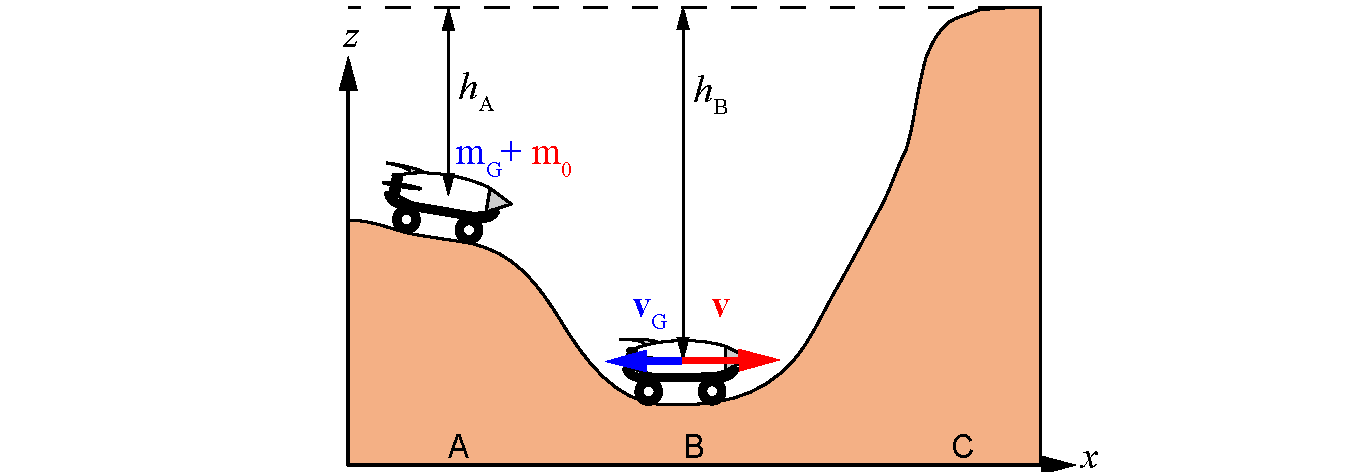
\includegraphics[width=\textwidth]{OberthEffAnalogie.pdf} 
	\caption[Analogie-Modell zum Oberth-Effekt.]{Analogie-Modell zum Oberth-Effekt (nach \cite{Blanco2019}).}
	\label{abb:adyn_rocket_analogy01}
\end{figure}

\medskip
%\hyperref[lsg:adyn_rocket_analogy]{\textcolor{blue} {$\rightarrow$ L�sungsvorschlag}}.\\
\linklsg\\%\href{FingerUeb2_AB.pdf#lsg:adyn_rocket_analogy}{\textcolor{blue} {$\rightarrow$ L�sungsteil}}.\\
\noindent\rule[1ex]{\textwidth}{0.5pt}
\end{prob}

%-----------------------------------------------------------------------------------------------------------

\begin{prob}  %�bung12
2
\einfach{adyn_manoevers1}{Hohmann-Transfer}
Berechnen Sie die �bergangszeit f�r den Hohmann-Transfer als Funktion von $r_2/r_1$ und diskutieren Sie diese.\\
Erkl�ren Sie, warum $\Delta v$ f�r den Hohmann-Transfer in bestimmten Situationen gr��er sein kann als die \gls{vescape}, obwohl die Bahn ja noch eine geschlossene Kreisbahn bleibt.\\ 
Was k�nnen Sie zu $\Delta v$ sagen, wenn man den Bahnradius verkleinern will?

\medskip
%\hyperref[lsg:adyn_manoevers1]{\textcolor{blue} {$\rightarrow$ L�sungsvorschlag}}.\\
\linklsg\\%\href{FingerUeb2_AB.pdf#lsg:adyn_manoevers1}{\textcolor{blue} {$\rightarrow$ L�sungsteil}}.\\
\noindent\rule[1ex]{\textwidth}{0.5pt}
\end{prob}

\newpage
%-----------------------------------------------------------------------------------------------------------
\begin{prob}  %�bung13
\mittel{adyn_manoevers2}{Bielliptischer �bergang}

Zwei-Impuls-�bergang von Bahn mit Radius $r_1$ auf eine elliptische Bahn mit Radius $r_2$:
Da der Antriebsbedarf $\Delta v$ beim Hohmann-Transfer in bestimmten F�llen sehr gro� sein kann, kann man �berlegen, ob es nicht g�nstiger ist, dass Raumschiff zun�chst auf die \gls{vescape} zu beschleunigen und dann wieder abzubremsen. Zeigen Sie, dass das in der Tat so sein kann. Was ist der Nachteil eines solchen Man�vers?

\medskip
%\hyperref[lsg:adyn_manoevers2]{\textcolor{blue} {$\rightarrow$ L�sungsvorschlag}}.\\
\linklsg\\%\href{FingerUeb2_AB.pdf#lsg:adyn_manoevers2}{\textcolor{blue} {$\rightarrow$ L�sungsteil}}.\\
\noindent\rule[1ex]{\textwidth}{0.5pt}
\end{prob}

%-----------------------------------------------------------------------------------------------------------
\begin{prob}  %�bung14
\einfach{adyn_manoevers3}{Hohmann-Oberth-Edelbaum-Transfers aus dem Orbit nach $\infty$}
Berechnen Sie Antriebsbedarfe und Energiegewinne eines Raumschiffs f�r die verschiedenen impulsiven Man�ver. F�r welchen Transfer w�rden Sie sich entscheiden, wenn der Treibstoffvorrat begrenzt ist?\\
Berechnen Sie die Flugzeiten des Raumschiffs bei den verschiedenen impulsiven Man�vern, bis das Raumschiff eine Entfernung des 50-, 100- \bzw 200-fachen des Radius~$r_1$ der anf�nglichen Umlaufbahn hat.

\medskip
%\hyperref[lsg:adyn_manoevers3]{\textcolor{blue} {$\rightarrow$ L�sungsvorschlag}}.\\
\linklsg\\%\href{FingerUeb2_AB.pdf#lsg:adyn_manoevers3}{\textcolor{blue} {$\rightarrow$ L�sungsteil}}.\\
\noindent\rule[1ex]{\textwidth}{0.5pt}
\end{prob}

%-----------------------------------------------------------------------------------------------------------
\begin{prob}  %�bung15
\schwierig{adyn_manoevers4}{Lambert-Problem}
Das Lambert-Problem wird heute meist in folgender Form geschrieben:
\begin{align}
  \Delta t &= \sqrt{\frac{a^3}{\mu}} \,\lek\alpha-\sin\alpha-\lk \beta -\sin\beta\rk \rek \,, \label{adyn_lambert_lsg01}
\end{align}
worin
\begin{align}
  \sin\lk \frac{\alpha}{2} \rk = \sqrt{\frac{s}{2a}}\,,~~~~~\sin\lk \frac{\beta}{2} \rk = \sqrt{\frac{s-c}{2a}}\, \label{adyn_lambert_lsg02}
\end{align}
Funktionen des gesuchten Bahnparameters $a$ und der bekannten geometrischen Gr��en $s$ und $c$ (siehe \figref{adyn_lambert_lsg01}) sind.
Diese Formulierung basiert auf der Kepler-Gleichung. 
Leiten Sie die Gleichung \eqref{adyn_lambert_lsg01} aus der Kepler-Gleichung her und l�sen Sie die Gleichung nach dem Bahnparameter $a$ mit Hilfe der Bisektionsmethode. Zur Anwendung der Methode siehe auch \probref{adyn_manoevers5} und \probref{adyn_manoevers6}, sowie die Literatur \cite{Izzo2015}.

\begin{figure}[H]
	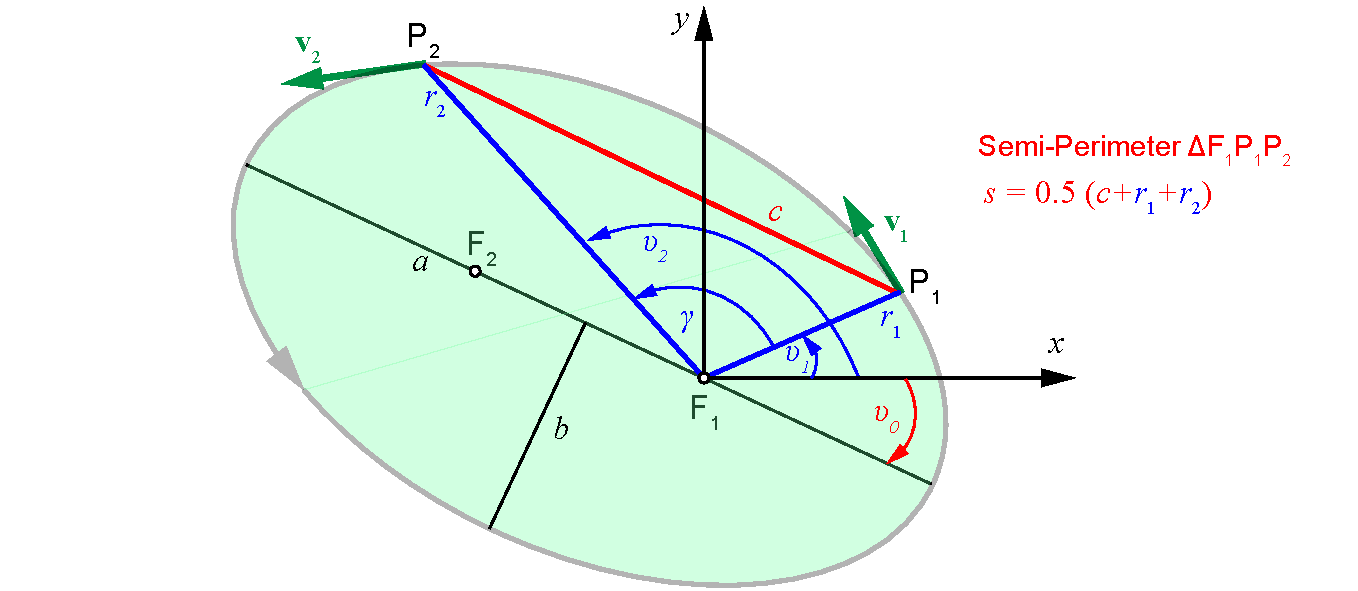
\includegraphics[width=\textwidth]{LambertProblem02Geometrie.pdf} 
	\caption[Geometrie des Lambert-Problems.]{Geometrie des Lambert-Problems.}
	\label{abb:adyn_lambert_lsg01}
\end{figure}

\medskip
%\hyperref[lsg:adyn_manoevers4]{\textcolor{blue} {$\rightarrow$ L�sungsvorschlag}}.\\
\linklsg\\%\href{FingerUeb2_AB.pdf#lsg:adyn_manoevers4}{\textcolor{blue} {$\rightarrow$ L�sungsteil}}.\\
\noindent\rule[1ex]{\textwidth}{0.5pt}
\end{prob}

%-----------------------------------------------------------------------------------------------------------
\begin{prob}  %�bung16
\schwierig{adyn_manoevers5}{Venus- und Mars-Fl�ge}
Benutzen Sie die L�sungsmethode des Lambert-Problems aus \probref{adyn_manoevers4}, um nun Venus- und Marsfl�ge aus einer Parkbahn um die Erde zu konzipieren. 
\begin{itemize}
	\item Berechnen Sie zun�chst die minimal m�gliche Transferzeit f�r ein gewisses Startdatum (\zb 18.6.2023). Diese wird durch einen parabolischen Orbit erreicht. \\
	\item Berechnen Sie nun f�r dieses Startdatum die Bahn f�r eine vorgegebene Flugzeit von 158 Tagen (zur Venus) \bzw 115 Tagen (zum Mars). \\
Benutzen Sie f�r Ihre Rechnungen die Werte aus der Tabelle \ref{tab:hm_bahnparameter} im Kapitel \ref{kap:hm_tabellen} der Himmelsmechanik. Hinweis: Sie k�nnen auch die Mittelpunktsgleichung\index{Mittelpunktsgleichung} \eqref{eq:hm_mpglg_r/a} aus \kap{hm_mpg} f�r eine einfache N�herung der elliptischen Bahnen von Mars und Venus verwenden.
\end{itemize}
Zusatzaufgabe: Suchen Sie ein optimales Startfenster f�r den Flug zum Mars aus. Wodurch ist dieses gekennzeichnet? Betrachten Sie dabei zwei F�lle:
	\begin{enumerate} [a)]
		\item Sie wollen nur einen Rover auf den Mars schaffen und zwar mit minimalen Treibstoffbedarf.
		\item Sie wollen mit Ihrer Crew auch m�glichst schnell wieder zur Erde zur�ck. Gehen Sie von realistischen Treibstoffvorr�ten aus. 
	\end{enumerate}

\medskip
%\hyperref[lsg:adyn_manoevers5]{\textcolor{blue} {$\rightarrow$ L�sungsvorschlag}}.\\
\linklsg\\%\href{FingerUeb2_AB.pdf#lsg:adyn_manoevers5}{\textcolor{blue} {$\rightarrow$ L�sungsteil}}.\\
\noindent\rule[1ex]{\textwidth}{0.5pt}
\end{prob}

%-----------------------------------------------------------------------------------------------------------
\begin{prob}  %�bung17
\mittel{adyn_manoevers6}{Abfang ballistischer Raketen}
Benutzen Sie die L�sungsmethode des Lambert-Problems aus \probref{adyn_manoevers4}, um ein Abfangman�ver zu berechnen.\\
Berechnen Sie das Geschwindigkeitsbudget, die Trajektorie und die Flugzeit einer Abfangrakete f�r eine interkontinentale ballistische Rakete (\textit{ICBM - \underline{I}nter-\underline{C}ontinental \underline{B}allistic \underline{M}issile}).\\
Die Abfangrakete befindet sich zum Zeitpunkt der Ortung bei:
\begin{align*}
	  \vec{r}(t_1)  = \vec{r}_1 = [6000, 3500, 0]\,\, \SI{}{\km}\,,~~~~
		\dot{\vec{r}}(t_1)  = \vec{v}_1 = [-2.5, 6.5, 2.5]\,\, \SI{}{\km\per\second}
\end{align*}
Die ICBM wurde getrackt mit:
\begin{align*}
	  \vec{R}(t_1)  &= \vec{R}_1 = [12250.0, 10250.0, 2000.0]\,\,\SI{}{\km}\,, ~~~~
		\dot{\vec{R}}(t_1) &= \vec{V}_1 = [-3.5, 1.0, 0] \,\,\SI{}{\km\per\second}
\end{align*}
Die ICBM soll binnen 30 min abgefangen werden und zwar bevor sie eine Flugh�he von 100 km erreicht. Ist das m�glich?
Zusatz: K�nnen Sie sagen, von wo die Rakete gestartet ist und wo sie ohne Abfang einschlagen w�rde?

\medskip
%\hyperref[lsg:adyn_manoevers6]{\textcolor{blue} {$\rightarrow$ L�sungsvorschlag}}.\\
\linklsg\\%\href{FingerUeb2_AB.pdf#lsg:adyn_manoevers6}{\textcolor{blue} {$\rightarrow$ L�sungsteil}}.\\
\noindent\rule[1ex]{\textwidth}{0.5pt}
\end{prob}


%-----------------------------------------------------------------------------------------------------------
\begin{prob}  %�bung18
\mittel{adyn_manoevers7}{Mondflug mit Ionenstrahltriebwerk}
L�sen Sie Bewegungsgleichung \eqref{eq:adyn_ionentr_01} numerisch f�r ein Triebwerk mit kontinuierlichem Schub f�r den Transfer aus einem LEO in einen GEO.\\
Parameter: $r_1= \SI{1000}{\km} + R_\text{E}$, $r_2 = \SI{35786}{\km} + R_\text{E}$, Schub $F_\text{S}= \SI{0.5}{\newton}$, Anfangsmasse $m_0= \SI{10000}{\kg}$, Massenaussto� $\dot{m}_\text{R} = \SI{3e-3}{\kg\per\second}$.\\

Berechnen Sie die Zeitdauer und Bahn f�r einen Mondflug mit einem Ionenstrahltriebwerk. Reduzieren Sie die Triebwerksleistung kontinuierlich so, dass diese bei einem Erreichen eines Abstands von der Erde, der dem Abstand des Lagrange-Punkts $\text{L}_1$ zwischen Erde und Mond entspricht, nahe Null wird. Vergleichen Sie mit dem Hohmann-Transfer.

\medskip
%\hyperref[lsg:adyn_manoevers7]{\textcolor{blue} {$\rightarrow$ L�sungsvorschlag}}.\\
\linklsg\\%\href{FingerUeb2_AB.pdf#lsg:adyn_manoevers7}{\textcolor{blue} {$\rightarrow$ L�sungsteil}}.\\
\noindent\rule[1ex]{\textwidth}{0.5pt}
\end{prob}

%-----------------------------------------------------------------------------------------------------------
\begin{prob}  %�bung19
\mittel{adyn_SOI}{Einflusssph�re - Sphere of Influence SOI}
Berechnen Sie die Radien der Einflusssph�ren der Planeten unseres Sonnensystems und vergleichen Sie mit dem Hill-Radius\index{Hill-Sph�re}, den wir in \probref{hm_hill_sphere} berechnet hatten. Worin unterscheiden sich die Radien? Wann muss man welchen heranziehen?

\medskip
%\hyperref[lsg:adyn_SOI]{\textcolor{blue} {$\rightarrow$ L�sungsvorschlag}}.\\
\linklsg\\%\href{FingerUeb2_AB.pdf#lsg:adyn_SOI}{\textcolor{blue} {$\rightarrow$ L�sungsteil}}.\\
\noindent\rule[1ex]{\textwidth}{0.5pt}
\end{prob}

%-----------------------------------------------------------------------------------------------------------

\begin{prob}  %�bung20
\mittel{adyn_swingby01}{Gravity-Assist-Man�ver - Analytische L�sung}
Finden Sie die analytischen L�sungen f�r $v_2$, $\Delta v = v_2 -v_1$ und $\gamma_2$ als Funktion der Eingangsparameter $v_1,\,v_\text{P},\,\gamma_1$. 
Finden Sie eine Beziehung f�r den Geschwindigkeits- und Energiegewinn beim Gravity-Assist-Man�ver und berechnen Sie die in der Tabelle \ref{tab:adyn_results_swingby}
in \kap{adyn_gravity_assist} angegebenen Werte f�r die theoretisch maximal erreichbaren Ablenkungen~$\vartheta'$ f�r die Planeten unseres Sonnensystems bei einem (unrealistischen) perizentralen Abstand von genau dem Planetenradius und einer typischen Einfluggeschwindigkeit von $v_1{}'= \SI{13.0}{\km\per\second}$. 

\medskip
%\hyperref[lsg:adyn_swingby01]{\textcolor{blue} {$\rightarrow$ L�sungsvorschlag}}.\\
\linklsg\\%\href{FingerUeb2_AB.pdf#lsg:adyn_swingby01}{\textcolor{blue} {$\rightarrow$ L�sungsteil}}.\\
\noindent\rule[1ex]{\textwidth}{0.5pt}
\end{prob}

%-----------------------------------------------------------------------------------------------------------

\begin{prob}  %�bung21
\einfach{adyn_swingby03}{Gravity-Assist-Man�ver - Simulation} 
Erstellen Sie in \matlab{} eine Simulation eines Gravity-Assist-Man�ver im Schwerefeld des Jupiters. \\

\medskip
%\hyperref[lsg:adyn_swingby03]{\textcolor{blue} {$\rightarrow$ L�sungsvorschlag}}.\\
\linklsg\\%\href{FingerUeb2_AB.pdf#lsg:adyn_swingby03}{\textcolor{blue} {$\rightarrow$ L�sungsteil}}.\\
\noindent\rule[1ex]{\textwidth}{0.5pt}
\end{prob}


%-----------------------------------------------------------------------------------------------------------

\newpage
\subsection{�bungen zu Rendezvous im Weltall}

\begin{prob}  %�bung22
\mittel{adyn_rendezvous01}{Rendezvous ISS und Raumtransporter}
Berechnen Sie, wie das Weltraum-Rendezvous zwischen der ISS und einem Raumtransporter stattfinden k�nnte. Ab welcher Entfernung kann die Bodenstation dem Kommandanten des Raumtransporters die Anweisung zur direkten manuellen Ansteuerung nach Sicht geben?

Gehen Sie von einer initial leicht elliptischen Bahn des Raumtransporters aus. Die gro�e Halbachse stimmt mit dem Radius der (nahezu) kreisf�rmigen Bahn der ISS �berein und die Exzentrizit�t betr�gt $e=0.035$. Beim Perig�um der Raumtransporterbahn haben die beiden Weltraumsysteme die gleiche wahre Anomalie.\\

Berechnen Sie auch numerisch f�r den Fall einer gro�er Elliptizit�t von $e=0.2$ die Bahnbeobachtung eines Raumschiffs von einer Raumstation aus der Kepler-L�sung, der L�sung aus der vollen Lagrange-Gleichung und zum Vergleich aus den CW-Gleichungen. Erkl�ren Sie Ihrer Ergebnisse.\\

\medskip
%\hyperref[lsg:adyn_rendezvous01]{\textcolor{blue} {$\rightarrow$ L�sungsvorschlag}}.\\
\linklsg\\%\href{FingerUeb2_AB.pdf#lsg:adyn_rendezvous01}{\textcolor{blue} {$\rightarrow$ L�sungsteil}}.\\
\noindent\rule[1ex]{\textwidth}{0.5pt}
\end{prob}
%-----------------------------------------------------------------------------------------------------------

\begin{prob}  %�bung23
\mittel{adyn_rendezvous02}{Rendezvous Apollo 11 CM und LM}
Berechnen Sie mit den Daten aus \kap{adyn_rendezvous_apollo11} und in der N�herung, dass die Bahnen von LM und CSM Kreisbahnen sind, wie das Weltraum-Rendezvous zwischen dem LM und dem CSM von Apollo 11 stattfand. Was k�nnen Sie �ber die Zeitabh�ngigkeit und die Genauigkeit des Zielwinkels des TPI-Burn sagen? 
Welcher Antriebsbedarf ist f�r den TPI-Burn notwendig? Ber�cksichtigen Sie dabei die Geschwindigkeit des LM vor dem TPI-Burn.\\
K�nnen Sie erkl�ren, warum der Astronaut Collins �ber die letzte Phase des "`geraden"' Anflugs etwas verwundert war?\\

\medskip
%\hyperref[lsg:adyn_rendezvous02]{\textcolor{blue} {$\rightarrow$ L�sungsvorschlag}}.\\
\linklsg\\%\href{FingerUeb2_AB.pdf#lsg:adyn_rendezvous02}{\textcolor{blue} {$\rightarrow$ L�sungsteil}}.\\
\noindent\rule[1ex]{\textwidth}{0.5pt}
\end{prob}

%-----------------------------------------------------------------------------------------------------------

\begin{prob}  %�bung24
\mittel{adyn_rendezvous03}{Planung einer Apollo Mission - \emph{Free Return Trajectory}}

Bei jeder der Apollo-Missionen zum Mond gab es eine besondere Sicherheitsma�nahme. F�r den Fall, dass die Mission aus irgendeinem Grund nicht so wie geplant durchgef�hrt werden konnte, wurde die Flugbahn des Apollo-Raumschiffs so geplant, dass es in einer freien R�ckflugbahn (\emph{Free Return Trajectory}) auf einer sogenannten \textit{slingshot trajectory} um den Mond herum "`geschleudert"' und nur durch die Gravitationskr�fte von Mond und Erde zur Erde zur�ckkehren w�rde. 
%In der Apollo 8 Mission wurde diese \textit{Free Return Trajectory} durch drei kurze Burns entsprechend angepasst.  Der erste Burn brachte Apollo 8 auf eine elliptische Umlaufbahn um den Mond, der zweite auf eine kreisf�rmige.  Apollo 8 umkreiste den Mond zehnmal und wurde dann nach einem dritten Burn wieder auf eine \textit{Free Return Trajectory} zur�ck zur Erde gebracht.  

Bei Apollo 13, der urspr�nglich dritten geplanten Mondlandemission, explodierte nach 56 Stunden Flugzeit ein Sauerstofftank an Bord des Raumschiffs. Das Raumschiff hatte nicht genug Treibstoff, um umzukehren und nach Hause zu fliegen. Es gab keine andere Wahl, als den Flug zum Mond fortzusetzen und auf der \textit{Free Return Trajectory} zur Erde zur�ckzukehren. Ohne die implizit eingebaute Sicherheitsma�nahme w�re das �berleben der Besatzung von Apollo 13 nicht m�glich gewesen.\\

Erstellen Sie zun�chst unter vereinfachenden Annahmen, dass  der Flug in der Mondbahnebene um die Erde stattfinden soll und dass nur die SOIs (\probref{adyn_SOI}) von Erde und Mond ber�cksichtigt werden sollen,  mittels der Methode des \textit{Patched-Conic-}N�herung\index{Patched-Conic-N�herung} (siehe \kap{adyn_gravity_assist}) 
eine erste n�herungsweise Missionsplanung f�r den Flug zum Mond. Bei der \textit{Free Return Trajectory} soll ohne weiteren Treibstoffverbrauch (von minimalen Kurskorrekturen abgesehen) nach der translunaren Injektion (\textit{Trans Lunar Injection} - TLI) eine sichere R�ckkehr zur Erde gew�hrleistet sein.\\
Versuchen Sie dann mit den so gewonnenen Anfangsdaten eine numerische L�sung.\\
Hinweise:
\begin{itemize}
	\item Beginnen Sie in der Erdumlaufbahn und legen Sie eine Richtung und eine Anfangsgeschwindigkeit f�r Ihre TLI fest.
	\item Stellen Sie die Trajektorie und die Position des Mondes dar.
	\item Zeigen Sie die Abh�ngigkeit der Flugbahn von Variationen in der Startgeschwindigkeit und der Startrichtung. 
\end{itemize}
Zusatz:
\begin{itemize}
	\item Berechnen Sie das n�tige Geschwindigkeitsbudget und die daf�r n�tige Treibstoffmenge f�r die TLI.
	\item Planen Sie eine Kurskorrektur, die das Raumschiff aus der \textit{Free Return Trajectory} in eine Mondumlaufbahn von ca. 120 km H�he bringt und eine weitere, die die Sonde aus dieser wieder in eine \textit{Free Return Trajectory} zur�ck zur Erde bringt.
\end{itemize}


F�r interessierte Leser sei auf das Apollo Flight Journal unter \url{https://www.nasa.gov/history/afj/} sowie die lesenswerte Beschreibung des Physikhintergrunds der Apollo-Missionen in \cite{Lundy2001} verwiesen, in denen jeweils alle Phasen der Apollo Missionen im Detail beschrieben sind.

\medskip
%\hyperref[lsg:adyn_rendezvous03]{\textcolor{blue} {$\rightarrow$ L�sungsvorschlag}}.\\
\linklsg\\%\href{FingerUeb2_AB.pdf#lsg:adyn_rendezvous03}{\textcolor{blue} {$\rightarrow$ L�sungsteil}}.\\
\noindent\rule[1ex]{\textwidth}{0.5pt}
\end{prob}

%-----------------------------------------------------------------------------------------------------------



\newpage
\subsection{�bungen zu Starts aus der Erdatmosph�re und zum Wiedereintritt}
%-----------------------------------------------------------------------------------------------------------

%\begin{prob}  %�bung25
%\einfach{adyn_forces01}{Kr�fte im Weltall}
%Berechnen Sie die Gr��enordnungen der Kr�fte von Tabelle \ref{tab:adyn_forces01}.
%�berlegen Sie sich die Wirkungen der Kr�fte auf die Umlaufbahnen von Satelliten.\\
%
%\medskip
%%\hyperref[lsg:adyn_forces01]{\textcolor{blue} {$\rightarrow$ L�sungsvorschlag}}.\\
%\linklsg\\%\href{FingerUeb2_AB.pdf#lsg:adyn_forces01}{\textcolor{blue} {$\rightarrow$ L�sungsteil}}.\\
%\noindent\rule[1ex]{\textwidth}{0.5pt}
%\end{prob}
%

%-----------------------------------------------------------------------------------------------------------

\begin{prob}  %�bung25
\mittel{adyn_launch01a}{Bewegungsgleichungen f�r Raketenstart von Erdoberfl�che}

Leiten Sie die skalaren Bewegungsgleichungen \eqref{eq:adyn_launch01} f�r einen Raketenstart von der Erdoberfl�che aus \eqref{eq:adyn_launch_vec} her.
Gehen Sie dabei von einem erdfesten \KOS\ in ein mitbewegtes \KOS\ �ber und schreiben Sie die Bewegungsgleichung in nat�rlichen Koordinaten und in geeigneten kartesischen Koordinaten ($h-x$).\\

\medskip
%\hyperref[lsg:adyn_launch01a]{\textcolor{blue} {$\rightarrow$ L�sungsvorschlag}}.\\
\linklsg\\%\href{FingerUeb2_AB.pdf#lsg:adyn_launch01a}{\textcolor{blue} {$\rightarrow$ L�sungsteil}}.\\
\noindent\rule[1ex]{\textwidth}{0.5pt}
\end{prob}


%-----------------------------------------------------------------------------------------------------------

\begin{prob}  %�bung26
\schwierig{adyn_launch01}{Raketenstarts von verschiedenen Weltraumzentren}
Die mathematisch-physikalische Behandlung eines Raketenstarts unter Ber�cksichtigung aller Faktoren (Atmosph�re, geographischer Ort der Startrampe, gew�nschte Bahn/Orbit, Nutzlast \usw) ist eine ziemlich komplexe Aufgabe, die letztendlich nur numerisch zu l�sen ist. Man kann mit den Erkenntnisse aus \kap{adyn_launch}
aber einige grunds�tzliche �berlegungen anstellen und Absch�tzungen machen, bevor man an die numerische Behandlung geht.\\
%Nach \figref{adyn_launch01} k�nnen wir den Flug eines Raumschiffs vom Start auf der Erdoberfl�che aus bis zum gew�nschten Orbit in 3 Phasen unterteilen:
%\begin{enumerate}
	%\item Schubphase
	%\item Freie Trajektorie (auch \textit{coasting phase} genant)
	%\item Gegebenenfalls eine Kurskorrektur (Burn) in den finalen, gew�nschten Orbit. 
%\end{enumerate}
In der �bung sollen folgende Aspekte behandelt werden:
\begin{itemize}
	\item Die Dynamik der Schubphase und den notwendigen Treibstoffbedarf  \bzw das Geschwindigkeitsbudget f�r das Erreichen eines bestimmten Orbits. Wir unterscheiden dabei den Fall des sogenannten \textit{Direct to Orbit} Transfers und des Transfers �ber eine Hohmann-Transferbahn mit anschlie�ender Kurskorrektur.
	\item Berechnung des Startverlaufs im mitbewegten \KOS{} nach \kap{adyn_launch} \bzw \probref{adyn_launch01a}.
	\item Festlegung des zeitlichen Startfensters und der Startrichtung (Startazimut) f�r den Start von verschiedenen Raumfahrtzentren im mitbewegten \KOS{} sowie im Inertialsystem.
	\item Komplette 3D-Trajektorienberechung der Startphase bis in den erdnahen Orbit.
\end{itemize}
Aufgabenstellungen:
\begin{enumerate}
\item Formulieren Sie eine allgemeine Optimierungsstrategie f�r einen Raumschiffstart in einen erdnahen Orbit. F�r die frei Trajektorie nehmen Sie einen Hohmann-Transfer an. Benutzen Sie auch die Ergebnisse von \kap{ady_reentry_conditions}. 
\item Berechnen Sie numerisch die Startphase einer dreistufigen Rakete (Ariane-1) im durch $\vec{t},\, \vec{n}$ und \vec{h} definierten mitbewegten \KOS. Ber�cksichtigen Sie den Drag und die Nickkorrektur. Legen Sie die Parameter so fest, dass die Rakete in eine Erdumlaufbahn von \ca 300 km H�he gelangt.
\item Zeigen Sie, dass man von einem Startort mit der geographischen Breite $\varphi_0$ ohne (treibstoffintensive) Bahnman�ver im Weltraum keine Orbits mit Inklinationen $i$ kleiner als $\varphi_0$ erreichen kann. Geben Sie auch eine physikalische Erkl�rung. Berechnen Sie f�r einen Raumschiffstart zur ISS jeweils Startfenster und Startazimut von Cape Canaveral, Baikonour und Kourou aus.
\item Berechnen Sie numerisch die 3D-Trajektorien im geozentrischen \KOS\ (Inertialsystem) f�r einen Raumschiffstart in eine Erdparkbahn von \ca 300 km jeweils von Cape Canaveral, Baikonour und Kourou aus. Ber�cksichtigen Sie den Einfluss der Erdrotation, der atmosph�rischen Reibung, ebenso wie den Nickwinkel und das Startazimut.
Berechnen Sie die Bodenspur des Raumschiffs von Start bis zum erstmaligen Abschluss einer Erdumrundung. 
Vergleichen Sie die Startbedingungen von den drei Zentren.\\
Benutzen Sie dabei die Daten aus Tabelle \ref{tab:adyn_parameter_raketen} f�r die Ariane-1 Rakete.
\end{enumerate}

\medskip
%\hyperref[lsg:adyn_launch01]{\textcolor{blue} {$\rightarrow$ L�sungsvorschlag}}.\\
\linklsg\\%\href{FingerUeb2_AB.pdf#lsg:adyn_launch01}{\textcolor{blue} {$\rightarrow$ L�sungsteil}}.\\
\noindent\rule[1ex]{\textwidth}{0.5pt}
\end{prob}

%-----------------------------------------------------------------------------------------------------------

\begin{prob}  %�bung27
\mittel{adyn_reentry01}{Parameter des Wiedereintritts in die Erdatmosph�re}
Leiten Sie die Beziehungen \eqref{eq:adyn_reentry03} mit den Kenntnissen aus \kap{hm_abl_kepler} her.\\
Vergleichen Sie die Problemstellung mit dem Lambert-Problem. Worin liegt der Unterschied, was gibt es f�r Gemeinsamkeiten?\\

\medskip
%\hyperref[lsg:adyn_reentry01]{\textcolor{blue} {$\rightarrow$ L�sungsvorschlag}}.\\
\linklsg\\%\href{FingerUeb2_AB.pdf#lsg:adyn_reentry01}{\textcolor{blue} {$\rightarrow$ L�sungsteil}}.\\
\noindent\rule[1ex]{\textwidth}{0.5pt}
\end{prob}

%-----------------------------------------------------------------------------------------------------------

\newpage
\begin{prob}  %�bung28
\mittel{adyn_reentry02}{Auftrieb/Drag-Abh�ngigkeit bei Wiedereintritt in Erdatmosph�re}
Untersuchen Sie die Abh�ngigkeit des H�henverlaufs $h(t)$. des Geschwindigkeitsverlaufs $v(t)$, des Flight Path Angle $\gamma(t)$ und der Beschleunigung (Abbremsung) $a(t)$ als Funktion des Verh�ltnisses von Auftrieb zu Drag f�r verschiedene initiale FPA.\\

\medskip
%\hyperref[lsg:adyn_reentry02]{\textcolor{blue} {$\rightarrow$ L�sungsvorschlag}}.\\
\linklsg\\%\href{FingerUeb2_AB.pdf#lsg:adyn_reentry02}{\textcolor{blue} {$\rightarrow$ L�sungsteil}}.\\
\noindent\rule[1ex]{\textwidth}{0.5pt}
\end{prob}

%-----------------------------------------------------------------------------------------------------------
\begin{prob}  %�bung29
\mittel{adyn_reentry03}{Normierte Gleichungen f�r $v(h)$ und $\gamma(h)$ bei Wiedereintritt}
Leiten Sie die Beziehung \eqref{eq:adyn_reentry11} aus \eqref{eq:adyn_launch08} f�r den Wiedereintritt in die Erdatmosph�re her.\\

\medskip
%\hyperref[lsg:adyn_reentry03]{\textcolor{blue} {$\rightarrow$ L�sungsvorschlag}}.\\
\linklsg\\%\href{FingerUeb2_AB.pdf#lsg:adyn_reentry03}{\textcolor{blue} {$\rightarrow$ L�sungsteil}}.\\
\noindent\rule[1ex]{\textwidth}{0.5pt}
\end{prob}

%-----------------------------------------------------------------------------------------------------------
\begin{prob}  %�bung30
\einfach{adyn_reentry04}{ISS Stabilit�t - Absturz und Vergl�hen des Satelliten Tiangong-1}
\begin{enumerate}
\item\textbf{\textit{Magnetsturm und ISS-Bahn}}\\
Dass ein Raumschiff beim Umkreisen der Erde wegen der minimal vorhandenen Reibung st�ndig an H�he verliert, ist v�llig normal. Bei der ISS sind es normalerweise \ca 100 Meter pro Tag. Berechnen Sie die mit einer geeigneten N�herungsrechnung die effektive Fl�che der ISS, die sich aus der normalen H�henverlustrate bei 420 km ergibt.
Wenn alle Systeme der ISS pl�tzlich ausfallen w�rden, wie lange w�rde es dauern, bis die ISS zum Absturz k�me?\\
W�hrend der heftigen Magnetst�rme im November 2004 sank die ISS bis zu 300 Meter pro Tag, so dass die Raumstation innerhalb weniger Tage um vier Kilometer an H�he verlor (\figref{adyn_ISS2004}).
Um wie viel gr��er war die Reibung durch den Magnetsturm im September? 

\begin{figure}[H]
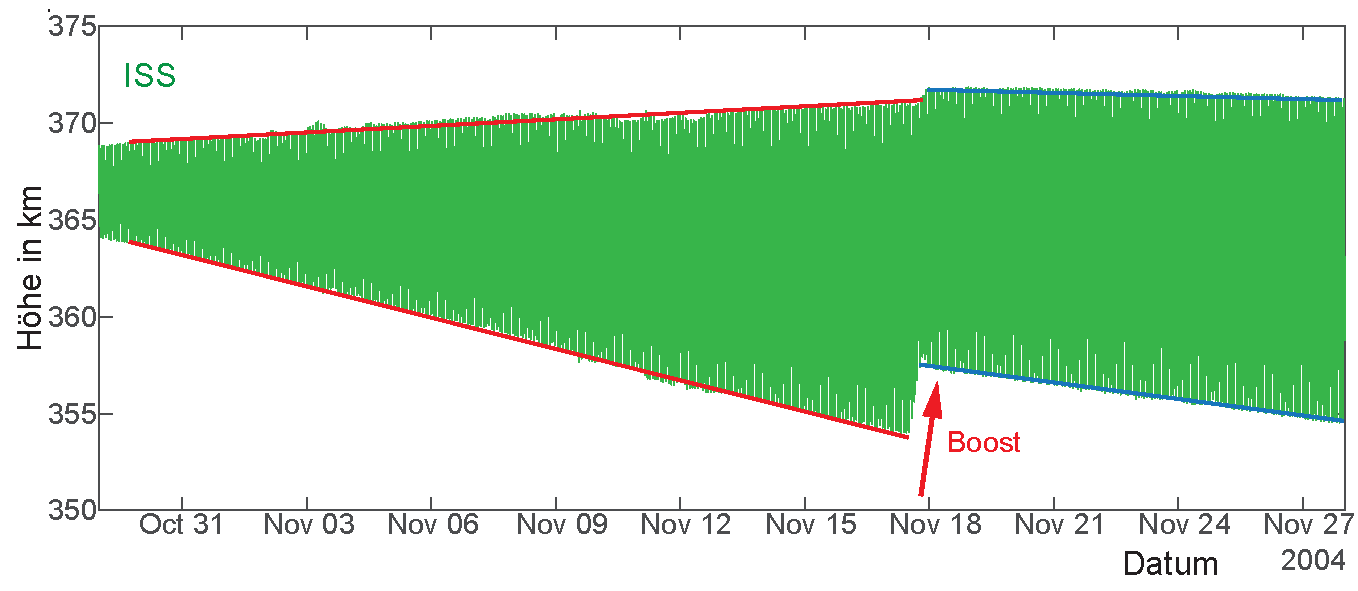
\includegraphics[width=\textwidth]{ISS2004.pdf}
\caption[H�he der Bahn der ISS im November 2004.]{H�henverlust der Bahn der ISS im November 2004 nach einem Magnetsturm. Daten von \cite{JPL2020}\, (siehe auch \mladyndref{ISS20004.txt}).}
\label{abb:adyn_ISS2004}
\end{figure}

\item \textbf{\textit{Der Absturz von Tiangong-1}}\\
Tiangong 1 (chinesisch f�r "`Himmelspalast 1"') war die erste Weltraumstation der Volksrepublik China. Der Start erfolgte mit einer Tr�gerrakete "`Langer Marsch"' am 29. September 2011. 
Das B�ro f�r bemannte Raumfahrt Chinas meldete am 21. M�rz 2016, dass die Ger�te an Bord von Tiangong-1 abgeschaltet wurden und dass sich seine Flugbahn im Laufe absenken und die Station in der Erdatmosph�re vergl�hen w�rde. Die Bahnh�he von Tiangong-1 verringerte sich zunehmend, der genaue Zeitpunkt des Wiedereintritts und damit der genaue Ort des Absturzes hing von der zum Teil unbekannten Dichte der Hochatmosph�re und von der Ausrichtung der Raumstation ab und lie� sich bis zuletzt nicht genau voraussagen.
Am 2. April 2018 um 00:16 Uhr UTC trat Tiangong-1 �ber dem S�dpazifik in die Erdatmosph�re ein und zerbrach in mehrere Teile (\figref{adyn_Tiangong2018}).
Untersuchen Sie mit einer geeigneten N�herungsrechnung den Absturz des Satelliten Tiangong-1 im Jahre 2018. Verwenden Sie die Daten aus \cite{JPL2020}\, (\mladyndref{Tiangong2018.csv}) \bzw \cite{Fiolhais2023, Pardini2019}.
\begin{figure}[H]
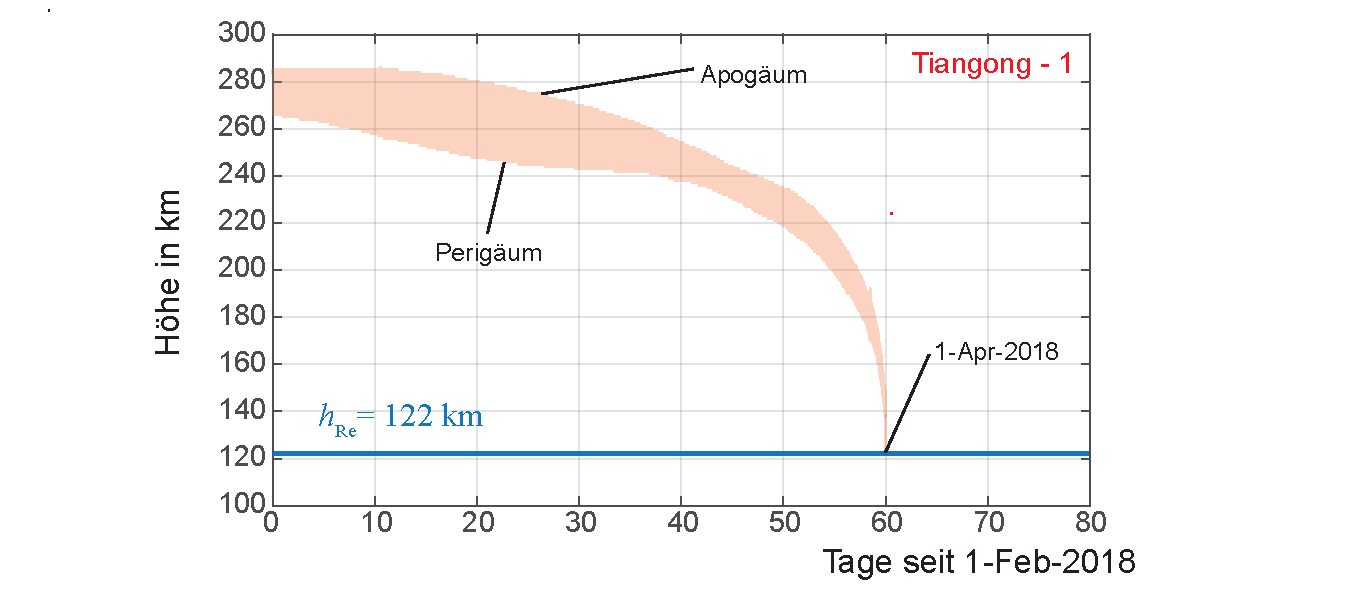
\includegraphics[width=0.95\textwidth]{Tiangong2018.pdf}
\caption[H�he der Bahn des chinesischen Satelliten Tiangong-1.]{H�he der Bahn des chinesischen Satelliten Tiangong-1 im Zeitraum Februar bis April 2018. Daten von \cite{JPL2020} (siehe auch \mladyndref{Tiangong2018.csv}).}
\label{abb:adyn_Tiangong2018}
\end{figure}

\item \textbf{\textit{Zusatzaufgabe 1}}\\

Berechnen Sie mit den Daten vom 05.03.2018 (\cite{JPL2020, Pardini2019} \bzw \mscr~\mladyndref{ISS2004.csv}) die Bahn der letzten Tage des Satelliten Tiangong-1 und die Bodenspur. Was ist Ihre Vorhersage? Vergleichen Sie mit dem tats�chlichen Ort des Vergl�hens (S�dpazifik $24.5\degree\,\text{S}, \, 151.1\degree\,\text{W}$).\\

\item \textbf{\textit{Zusatzaufgabe 2}}\\

Zeigen Sie numerisch wie extrem kritisch die Wiedereintrittsphase in einem solch einem Fall vom FPA $\gamma$ abh�ngt. Benutzen Sie die Ergebnisse von \probref{adyn_reentry03}.\\ 
\end{enumerate}

\medskip
%\hyperref[lsg:adyn_reentry04]{\textcolor{blue} {$\rightarrow$ L�sungsvorschlag}}.\\
\linklsg\\%\href{FingerUeb2_AB.pdf#lsg:adyn_reentry04}{\textcolor{blue} {$\rightarrow$ L�sungsteil}}.\\
\noindent\rule[1ex]{\textwidth}{0.5pt}
\end{prob}

%-----------------------------------------------------------------------------------------------------------
\begin{prob}  %�bung31
\einfach{adyn_BoatRocketModel}{Zur Entspannung}
Zum Abschluss zur Entspannung eine sch�ne Analogieaufgabe zwischen einer Rakete und einem Physiker als Bootsfahrer. Dieser will sich durch Abwerfen von Kokosn�ssen aus seinem Boot vorw�rts bewegen\footnote{Diese sch�ne Aufgabe geht auf \cite{Lagos2023} zur�ck}.\\
\figref{adyn_BoatRocketModel} zeigt die Situation des Bootsfahrers Leonardo, ohne Ruder und sonstigen Antrieb. Er hat lediglich $N$ Kokosn�sse der Masse $m_\text{K}$, die er jeweils mit einer Geschwindigkeit $v_\text{K}$ abwerfen kann. Sein Boot wiegt $m_\text{B}$, er selbst $m_\text{L}$. 
Zeigen Sie mit Hilfe des Impulserhaltungssatzes, dass das Problem �quivalent ist zu Raketengleichung und dass Sie f�r $N\rightarrow\infty$ und gleichzeitig  
$m_\text{K}\rightarrow 0$ tats�chlich die Raketengleichung erhalten.

\begin{figure}[H]
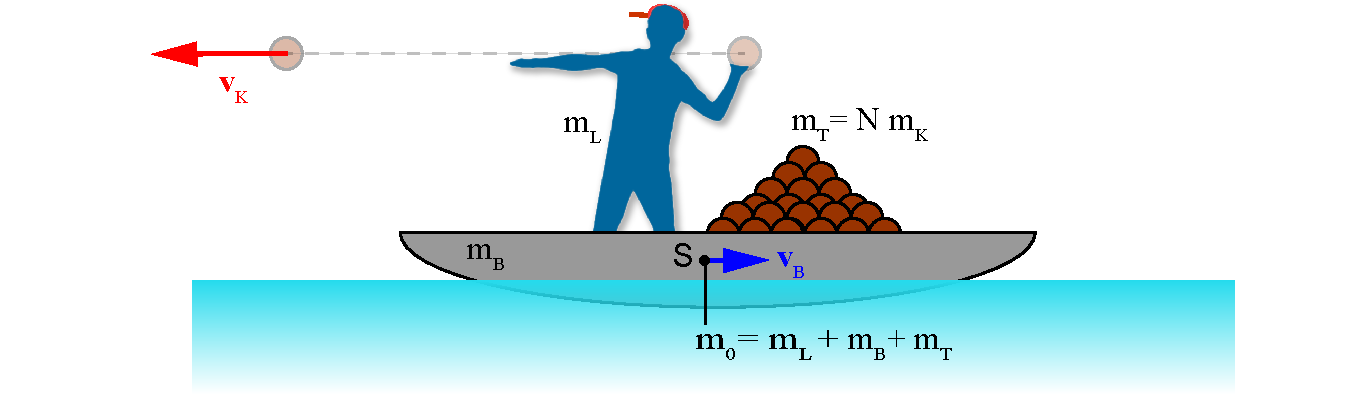
\includegraphics[width=\textwidth]{BoatRocketModel.pdf}
\caption[Diskretes Modell der Raketengleichung.]{Diskretes Modell der Raketengleichung.}
\label{abb:adyn_BoatRocketModel}
\end{figure}

\medskip
%\hyperref[lsg:adyn_BoatRocketModel]{\textcolor{blue} {$\rightarrow$ L�sungsvorschlag}}.\\
\linklsg\\%\href{FingerUeb2_AB.pdf#lsg:adyn_BoatRocketModel}{\textcolor{blue} {$\rightarrow$ L�sungsteil}}.\\
\noindent\rule[1ex]{\textwidth}{0.5pt}
\end{prob}


\newpage
\subsection{Weiterf�hrende Zusatzaufgaben und Probleme}

%-----------------------------------------------------------------------------------------------------------

\begin{prob}  %Zusatz1
\zusatz{adyn_launchinnovations}{Neue Ideen zum Flug ins Weltall}
Immer wieder gibt es Berichte zu alternativen und kosteng�nstigeren Methoden, Lasten von der Erde in den Weltraum zu bringen.
Besonders zwei Methoden haben in den letzten Jahren gro�e Aufmerksamkeit erreicht und auch entsprechendes Funding:
\begin{enumerate}
	\item Steinschleuder-Methode (englisch \textit{Spinlaunch}) \\
	Bei dieser relativ neuen, \ua von der Firma \textit{Spinlaunch} diskutierten Methode, wird mit einem rotierenden Massenbeschleuniger (einer Art Zentrifuge) eine geschossf�rmige Tr�gerrakete in gro�e H�hen katapultiert. Dort sollen die Triebwerke gez�ndet und die Nutzlast in eine Erdumlaufbahn gebracht werden. Dieses System soll weitaus kosteng�nstiger arbeiten als herk�mmliche Stufenraketen, ein erster Start wird f�r 2026 prognostiziert (\url{www.spinlaunch.com}, \cite{Krolle2022}).
	\item Weltraumfahrstuhl (englisch \textit{Space Elevator}) \\
	Die Idee dieser seit einigen Jahren \ua von der Firma \textit{Liftport} diskutierten Methode besteht darin, an einem Seil aus geeignetem Material Nutzlasten nach oben zu ziehen. Das Seil verl�uft vom �quator senkrecht nach oben �ber die geostation�re Bahn eines Satelliten hinaus und wird dort eventuell durch eine Gegenmasse abgeschlossen. (\url{www.liftport.com}, \cite{Aravind2007, Swan2013, Rauchhaupt2014}).
\end{enumerate}

Bewerten Sie diese Methoden, indem Sie einfache Absch�tzungen zur Realisierbarkeit machen. Was sind die Top-Probleme \bzw Herausforderungen. Welche Risiken sehen Sie?
K�nnen Sie eine Kostenabsch�tzung machen im Vergleich zu heutigen Kosten? SpaceX gibt heute $\SI{3000}{}$ USD pro kg Fracht an.\\
W�rden Sie investieren, in welches der beiden Projekte am ehesten?

\medskip
\linklsg\\%\hyperref[lsg:adyn_launchinnovations]{\textcolor{blue} {$\rightarrow$ L�sungsvorschlag}}.\\
\noindent\rule[1ex]{\textwidth}{0.5pt}
\end{prob}


%-----------------------------------------------------------------------------------------------------------

\begin{prob}  %Zusatz2
\zusatz{adyn_orbits_zusatz1}{Bahnparameter aus Bodenbeobachtungen (Ortsvektoren) }
Diese Aufgabe wurde aus \cite{Montenbruck2012} entnommen.\\
Berechnen Sie die Bahnparameter eines Satelliten f�r folgende Beobachtungen von der Station mit den geozentrischen Stationskoordinaten:\\
	$x_\text{B} = \SI{1344.143}{\km,}\,\, y_\text{B} = \SI{6068.601}{\km,}\,\,z_\text{B} = \SI{1429.311}{\km}\,.$  (Indien)\\
Die topozentrischen Messwerte f�r die indische Station sind:\\
	02.04.1999\,\, 00:30:00 UTC\,:\; $\mathcal{A} = 132.67\degree~\,,~h=32.44\degree~\,~  R_\text{S}=\SI{16945.45}{\km}$\,,\\
	02.04.1999\,\, 03:00:00 UTC\,:\; $\mathcal{A} = 123.08\degree~\,,~h=50.06\degree~\,~  R_\text{S}=\SI{37350.34}{\km}$\,.\\

\medskip
\linklsg\\%\hyperref[lsg:adyn_orbits_zusatz1]{\textcolor{blue} {$\rightarrow$ L�sungsvorschlag}}.\\
\noindent\rule[1ex]{\textwidth}{0.5pt}
\end{prob}

%-----------------------------------------------------------------------------------------------------------

\begin{prob}  %Zusatz3
\zusatz{adyn_orbits_zusatz2}{Bahnparameter aus Bodenbeobachtungen (Ortsvektoren) }
Berechnen Sie aus den in \probref{adyn_orbits3} berechneten topozentrischen Beobachtungsdaten zu den Zeiten 00:32 und 00:38 in G�rlitz nun umgekehrt die Bahnparameter.
Die Stationskoordinaten von G�rlitz sind: $\lambda = 15\degree$ O  und $\varphi=51\degree$ N.\\

\medskip
\linklsg\\%\hyperref[lsg:adyn_orbits_zusatz1]{\textcolor{blue} {$\rightarrow$ L�sungsvorschlag}}.\\
\noindent\rule[1ex]{\textwidth}{0.5pt}
\end{prob}



%-----------------------------------------------------------------------------------------------------------

\begin{prob}  %Zusatz4
\zusatz{adyn_manoevers8}{Marsflug mit Ionenstrahltriebwerk}
Konzipieren Sie einen Marsflug mit einem Ionenstrahltriebwerk. Seien Sie optimistisch und nehmen Sie eine Ausstr�mgeschwindigkeit von $v_\text{ion}=\SI{50}{\kilo\metre\per\second}$ und einen Anfangsschub von $\SI{50e-3}{\newton\per\kg}$ an. Das Raumschiff soll bereits in einer Parkbahn in 10000 km Abstand von der Mondoberfl�che kreisen. Welche Treibstoffmasse ist notwendig, was ist der gesamte Energiebedarf/Leistungsbedarf und mit welcher Flugzeit m�ssen Sie rechnen? Vergleichen Sie das mit einem Hohmann-Transfer \bzw der Flugzeit, die Sie in \probref{adyn_manoevers5} berechnet haben. \\
Was k�nnen Sie �ber das Nutzlastverh�ltnis sagen?\\
Hinweis: Gehen Sie analog zu \probref{adyn_manoevers7} vor und �berlegen Sie sich, welche sinnvollen N�herungen Sie f�r welchen Flugabschnitt machen k�nnen, um die numerische Rechnung zu vereinfachen und zu beschleunigen.

\medskip
%\hyperref[lsg:adyn_manoevers8]{\textcolor{blue} {$\rightarrow$ L�sungsvorschlag}}.\\
\noindent\rule[1ex]{\textwidth}{0.5pt}
\end{prob}


%-----------------------------------------------------------------------------------------------------------

\begin{prob}  %Zusatz5
\zusatz{adyn_swingby02}{Gravity-Assist-Man�ver - Allgemeiner Fall}
Betrachten Sie das GA-Man�ver im allgemeinen Fall, \dh dass die Bahnebene der Raumsonde und die Planetenebene nicht mehr �bereinstimmen (\figref{adyn_GA3dim}) und die
Bahnebene auch nicht mehr der Ekliptik entspricht. Geben Sie eine Berechnungsvorschrift f�r die Ausgangsparameter des GA-Man�vers in Matrixschreibweise an.
Finden Sie �ber eine vektorielle Definition des Streuparameters eine mathematische Formulierung f�r die jeweiligen F�lle des GA-Man�vers "`vor"' bzw. "`hinter"' einem Planeten und begr�nden Sie, warum sich daraus entweder $\vartheta' > 0$ oder $\vartheta' < 0$ ergibt.

\begin{figure}[H]
	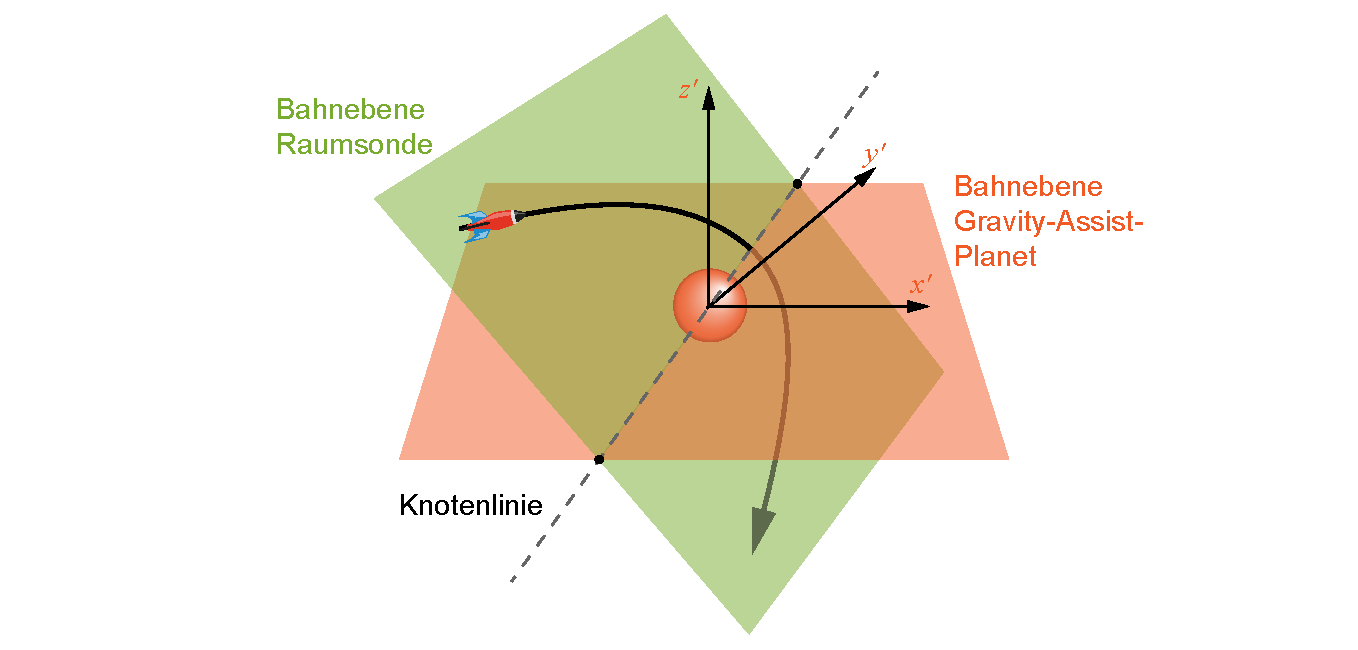
\includegraphics[width=\textwidth]{GravityAssist3D.pdf} 
	\caption[Geometrie des Gravity-Assist-Man�vers.]{Geometrie des Gravity-Assist-Man�vers (nichtkoplanarer Fall).}
	\label{abb:adyn_GA3dim}
\end{figure}
\medskip
\linklsg\\%\hyperref[lsg:adyn_swingby02]{\textcolor{blue} {$\rightarrow$ L�sungsvorschlag}}.\\
\noindent\rule[1ex]{\textwidth}{0.5pt}
\end{prob}


%-----------------------------------------------------------------------------------------------------------

\begin{prob}  %Zusatz6
\zusatz{adyn_swingby04}{Gravity-Assist-Man�ver - Zus�tzlicher Schub }
Berechnen Sie die Ausgangsparameter eines GA-Man�vers, bei dem die Raumsonde am Perizentrum noch einen Zusatzbetrag $\Delta v_\text{ext}$ aus den Treibstoffvorr�ten bekommt. Wie ver�ndern sich die Ausgangswerte zum Fall $\Delta v_\text{ext} = 0$ und zum Fall, wenn  $\Delta v_\text{ext}$ an den Punkten $\mathrm{P}_1$ \bzw  $\mathrm{P}_2$ zur Anwendung kommt. Diskutieren Sie Ihre Ergebnisse. 

\medskip
\linklsg\\%\hyperref[lsg:adyn_swingby04]{\textcolor{blue} {$\rightarrow$ L�sungsvorschlag}}.\\
\noindent\rule[1ex]{\textwidth}{0.5pt}
\end{prob}



%-----------------------------------------------------------------------------------------------------------

\begin{prob}  %Zusatz7
\zusatz{adyn_PSP01}{Flug der Parker Solar Probe - PSP}
Berechnen Sie die Bahn der PSP �ber die Patched-Conic-N�herung. Benutzen Sie dabei die Werte aus \kap{adyn_interplanetary_flights} und f�r die Anfangswerte der Bahn Daten der Horizon-Webseite des Jet Propulsion Lab \url{https://ssd.jpl.nasa.gov/horizons.cgi}. Die Daten sind  im File \mladyndref{PSP.csv} hinterlegt. F�r die Planeten k�nnen die Bahnen mit den Methoden aus dem \kap{hm_bahnen_hk_ss} in der Himmelsmechanik berechnet werden. \\
Ebenso sch�tze man ab, ob der Treibstoffvorrat dieser Sonde von $\SI{3650}{\kg}$ mit optimistischen  $v_\text{G} = \SI{4}{\km\per\second}$ ausgereicht h�tte, JUICE aus einer elliptischen Bahn um die Sonne (Perihelabstand von etwa $\SI{1}{AE}$) zum Jupiter zu bringen. Hinweis: Die gesamte mitgef�hrte Treibstoffmasse von JUICE betrug $\SI{3650}{\kg}$, die Strukturmasse und Nutzlast zusammen $\SI{2700}{\kg}$. Als Hinweis sei erw�hnt, dass die Startrakete eine Ariane 5 war, die f�r Transporte in den geostation�ren Orbit optimiert ist und die mit der Nutzlast von $\SI{6.3}{\tonne}$ beim Start voll ausgelastet war.

\medskip
%\hyperref[lsg:adyn_PSP01]{\textcolor{blue} {$\rightarrow$ L�sungsvorschlag}}.\\
\noindent\rule[1ex]{\textwidth}{0.5pt}
\end{prob}


%-----------------------------------------------------------------------------------------------------------

\begin{prob}  %Zusatz8
\zusatz{adyn_pertubations}{Gest�rte Satellitenbahnen - Grundideen der St�rungstheorie}
Berechnen Sie die �nderungen der Bahnparameter eines Satelliten (\bzw eines beliebigen Himmelsk�rpers) bei Vorhandensein einer beliebigen St�rkraft $\vec{F}_\text{S}$ zus�tzlich zum Zentralkraftfeld der Erde (\bzw des Zentralk�rpers) numerisch und durch analytische N�herungsformeln.
Benutzen Sie dabei das mit dem Satelliten mitbewegte Koordinatensystem~\vec{PQR}.

F�r die numerische Methode k�nnen Sie zwei verschiedene Methoden verwenden (vgl. auch \figref{adyn_pertubations01}):
\begin{enumerate}
	\item \textbf{Methode von Cowell}\footnote{Philip Herbert Cowell (1870 -- 1949) war ein britischer Astronom, der mit der nach ihm benannten Methode zur L�sung von Differentialgleichungen in rechtwinkligen Koordinaten einen bedeutenden Beitrag zur Berechnung der Bahnen von Himmelsk�rpern lieferte.}\indexp{Cowell, Philip Herbert}
	
	Die Cowell-Methode, Anfang des 20. Jahrhunderts ver�ffentlicht, besteht darin, dass man einfach die beiden Bewegungsgleichungen f�r die gest�rten Bahn $\vec{\rho}(t)$ und eine Referenzbahn $\vec{r}(t)$ (die sogenannte \gls{Oskulation}) \index{Bahn!oskulierende} \cite{Montenbruck1999} aufschreibt und diese dann simultan numerisch integriert.\\

	\item \textbf{Methode von Encke}\footnote{Johann Franz Encke (1791 -- 1865) war ein deutscher Astronom, der unter anderem die nach ihm benannte Enckesche Teilung des Saturnrings entdeckte. Er bestimmte die Bahnen vieler Kometen und Asteroiden mit hoher Genauigkeit, ebenso wie die Astronomische Einheit.}\indexp{Encke, Johann Franz}

	Die Encke-Methode, die bereits 1857 ver�ffentlicht wurde, besteht darin, dass man aus den beiden Bewegungsgleichungen f�r die gest�rten Bahn $\vec{\rho}(t)$ und die oskulierende Bahn $\vec{r}(t)$ eine Differentialgleichung f�r die Differenz $\vec{r}_\Delta (t)$ gewinnt und diese dann mit einem speziellen Verfahren numerisch integriert.
\end{enumerate}
	Beide Verfahren z�hlen zu den sogenannten speziellen St�rungstheorien, da letztendlich numerisch integriert werden muss.

	Alternativ kann man versuchen, analytisch �ber Reihenentwicklungen die zeitliche Variation der Bahnparameter aus den St�rbeschleunigungen abzuleiten. Dies ist erstmalig in einem ber�hmt gewordenen NASA-Report erfolgt \cite{NASA1968}. Man kann, dem dort dargelegten Prinzip folgend, f�r die Bahnparametervariationen $\D a/ \D t$, $\D e/ \D t$ \usw relativ kompakte Gleichungen herleiten und an diesen auch die Wirkung der unterschiedlichen St�rungen gut erkennen.
	
\begin{figure}[H]
	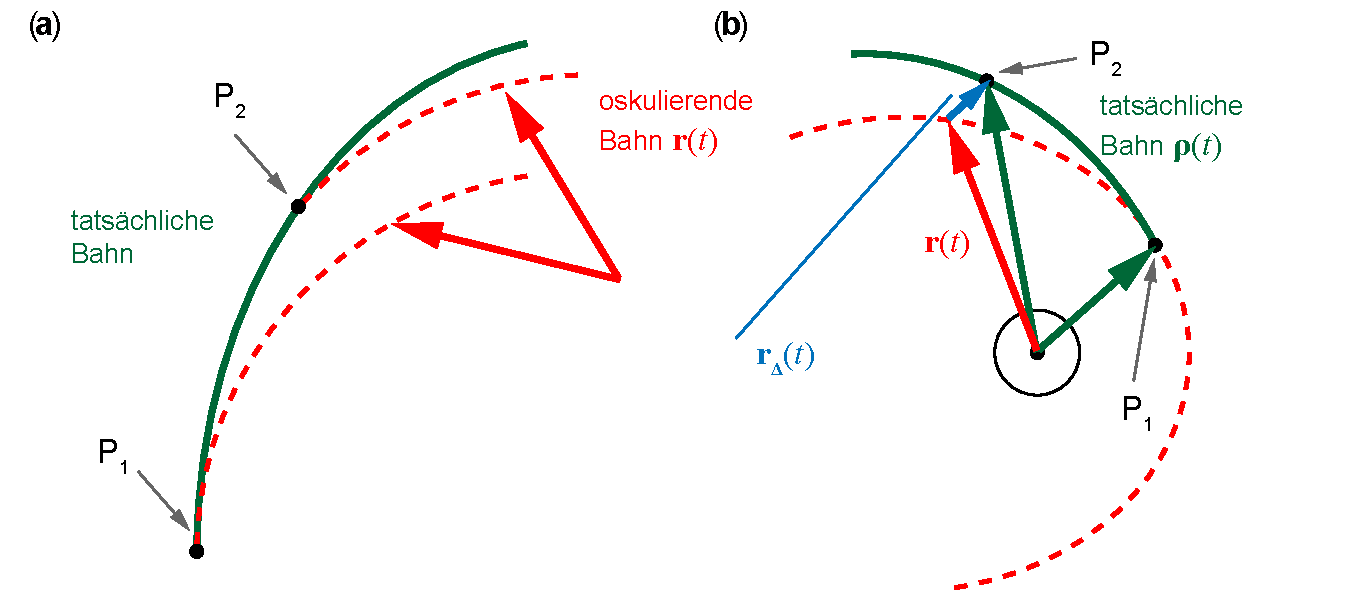
\includegraphics[width=\textwidth]{Stoerungsrechnung01.pdf} 
	\caption[Geometrie f�r die St�rungsrechnung.]{Geometrie f�r die St�rungsrechnung. \fa Definition der oskulierenden Bahn. \fb Definition von  $\vec{r}_\Delta (t)$ f�r die speziellen St�rungsrechnung nach der Methode von Encke.}
	\label{abb:adyn_pertubations01}
\end{figure}
\medskip
%\hyperref[lsg:adyn_PSP01]{\textcolor{blue} {$\rightarrow$ L�sungsvorschlag}}.\\
\noindent\rule[1ex]{\textwidth}{0.5pt}
\end{prob}

%-----------------------------------------------------------------------------------------------------------



 
%\clearpage
%\newpage
\subsection{\mscre -- Astrodynamik}\label{kap:adyn_matlabskripts}

Die \mscre befinden sich im MATLAB-Ordner \texttt{MatlabDateien/adyn},
die Hilfsfunktionen im dortigen Unterordner \texttt{Include\-folder} und Daten im Unterordner \texttt{Data}.
Es wird empfohlen, entweder die Skripte im GitHub Verzeichnis \githubSN zu benutzen oder sich die komplette Verzeichnisstruktur von \MKc~ runter zu laden und diese und auch das Arbeitsbuch im Hauptverzeichnis Fingeruebungen zu installieren. \\

Wir wollen noch einmal explizit darauf hinweisen, dass die \mscre prim�re der Vermittlung der physikalischen Modelle dienen und keinen Anspruch auf besonders elegante oder effiziente Programmierung erheben. Unser Buch ist ja kein Lehrbuch f�r \matlab-Programmierung. Uns ging es bewusst darum, dass die Skripte gut lesbar sind und das physikalische Modell bzw den physikalischen Gedankengang m�glichst klar abbilden.
Die Leser sind aufgerufen, die Programme nach Belieben zu verbessern und kompakter zu gestalten und diese auch ins GitHub Verzeichnis \githubSN zu stellen.

\subsubsection {Skripte zu Beispielen} \label{mls:adyn_kapitel} 
\begin{longtable}{p{0.34\textwidth}p{0.66\textwidth}}
\hline\noalign{\smallskip}
Skript & Beschreibung \\
\noalign{\smallskip}\svhline\noalign{\smallskip}
\mladynref{FlugzeitenMarsVenus.m}           & Programm berechnet die Flugzeiten f�r Hohmann-Ellipsen zu einem der Nachbar-Planeten (Venus, Mars) in der N�herung kreisf�rmiger Bahnen der Planeten.\\
\mladynref{GravityAssist01.m}               & Berechnet verschiedene Abh�ngigkeiten eines Gravity-Assist-Man�vers am Jupiter.\\
\mladynref{GravityAssist02.m}               & Berechnet verschiedene Abh�ngigkeiten der Gravity-Assist-Man�ver an den Planeten des Sonnensystems.\\
\mladynref{HohmannTransfer.m}               & Berechnet den Geschwindigkeitsbedarf f�r den Hohmann-Transfer als Funktion der Verh�ltnisse von Anfangs- und Endradius der kreisf�rmigen Erdumlaufbahnen von Satelliten und die Transferzeiten f�r interplanetare Hohman-Transfers.\\
\mladynref{Ionenantrieb01.m}                & Programm berechnet die Geschwindigkeitssch�be und die Bahnen/Flugzeiten f�r einen Ionenantrieb aus einem LEO in ein GEO im Vergleich zum Hohmann-Transfer (N�herungsl�sung).\\
\mladynref{LambertProblem01.m}              & Programm berechnet die Parameter der Ellipsenbahn f�r das Lambert-Problem �ber Iteration. Verwendet \mladyniref{LambertSolver1.m}\\
\mladynref{LambertProblem02.m}              & Programm berechnet die Parameter der Ellipsenbahn $a,\, e$ f�r das Lambert-Problem bei vorgegebener Geometrie f�r verschiedene ToF. Verwendet \mladyniref{LambertSolver2.m}\\
\mladynref{LambertProblem03.m}              & Programm berechnet die Parameter der Ellipsenbahn bzw. Hyperbelbahn f�r das allgemeine Lambert-Problem bei vorgegebenen Positionsvektoren 1 und 2 und der Richtung Bewegung, sowie der Flugzeit (ToF). Als Zentralk�rper ist entweder die Erde oder die Sonne angenommen. Verwendet \mladyniref{LambertSolver3.m}.\\
\mladynref{LMCSMApollo11.m}                 & Rendezvous von LM und CSM von Apollo 11 in der Mondumlaufbahn (Berechnung der Kinematik des Rendezvous �ber die Clohessy-Wiltshire-Gleichungen).\\
\mladynref{ParkerSolarProbe.m}              & Programm berechnet die einzelnen Gravity-Assist-Man�ver der Parker-Solar-Probe und simuliert die Bahn im Zeitraum von Start bis 2024.\\
\mladynref{Raketenstart01.m}                & Berechnet Start und Flug einer einstufigen Rakete von der Erdoberfl�che.\\
\mladynref{Raketenstart02.m}                & Programm berechnet Nutzlast-Antriebsverm�gen-Relation als Funktion des Strukturmassen-Verh�ltnisses.\\
\mladynref{Raketenstart03.m}                & Programm berechnet Nutzlast-Antriebsverm�gen-Relation f�r Ariane 1 und Saturn V.\\
\mladynref{RaketenstartReal.m}              & Programm berechnet Start einer einstufigen Rakete von der Erdoberfl�che unter Ber�cksichtigung von Reibung und Nickwinkel-Korrekturen.\\
\mladynref{ReentryNaeherungen.m}            & Programm berechnet die Dynamik des Wiedereintritts eines Raumschiffes in die Erdatmosph�re mit dem vollst�ndigen DGL-System in der N�herung $x,h \ll R_\text{E}$ und in den N�herungsl�sungen aus dem normierten DGL-System.\\
\mladynref{Rendezvous01.m}                  & Programm berechnet die Dynamik eines Weltall-Rendezvous eines Astronauten, der sich au�erhalb der Raumstation befindet mit der ISS. L�sung der Hill-Gleichungen und Clohessy-Wiltshire-Gleichungen (direkter Anflug mit verschiedenen Antriebsgeschwindigkeiten).\\
\mladynref{Rendezvous02.m}                  & Programm berechnet die Dynamik eines Weltall-Rendezvous eines Astronauten, der sich au�erhalb der Raumstation befindet mit der ISS. L�sung der Hill-Gleichungen und Clohessy-Wiltshire-Gleichungen (verschiedene Antriebsrichtungen).\\
\mladynref{Rendezvous03.m}                  & Berechnung der Kinematik eines Weltall-Rendezvous eines Targets und J�gers (L�sung �ber die Kepler-Gleichung bzw. die Clohessy-Wiltshire-Gleichungen).\\
\noalign{\smallskip}\svhline\noalign{\smallskip}
\end{longtable}

\subsubsection{Skripte zu �bungen} \label{mls:adyn_uebungen} %MLSkript�bungen
\begin{longtable}{p{0.34\textwidth}p{0.66\textwidth}}
\hline\noalign{\smallskip}
Skript & Beschreibung \\
\noalign{\smallskip}\svhline\noalign{\smallskip}
\mladynref{AlternativeRaketenGl.m}          & Berechnet die Raketengleichung nach einem diskreten Modell. \\
\mladynref{BahnparaBestimmung01.m}          & Berechnet die Bahnparameter von Satellitenbahnen um die Erde aus einem bekannten Orts- und Geschwindigkeitsvektor. \\
\mladynref{BiElliptischerTransfer.m}        & Berechnet Zwei-Impuls-�bergang von Bahn mit Radius $r_1$ auf eine elliptische Bahn (bielliptischer �bergang) mit Radius $r_2$.\\
\mladynref{FlugVenusParabelbahn.m}          & Programm berechnet die Parabel-Flugbahn einer Raumsonde zur Venus zu verschiedenen Startzeiten. Vorgegeben ist das Startdatum, gesucht ist das Ankunftsdatum mit dem schnellsten Transfer unabh�ngig vom notwendigen Antriebsbedarf.\\
\mladynref{FreReturTrajectorie01.m}         & Berechnet f�r verschiedene Parameter die Free Return Trajectorie um den Mond.\\
\mladynref{GravityAssistAnalytik.m}         & Analytische Formeln f�r Gravity-Assist-Man�ver und deren Auswertung.\\
\mladynref{GravityAssistSimulation.m}       & Programm simuliert die Streuung einer Raumsonde an einem Planeten (Gravity-Assist-Man�ver) im heliozentrischen KOS am Beispiel Jupiter.\\
\mladynref{IonenantriebMond.m}              & Programm berechnet die Geschwindigkeitssch�be und die Bahnen/Flugzeiten f�r einen Ionenantrieb aus einem LEO zum Mond im Vergleich zum Hohmann-Transfer.\\
\mladynref{Ionenantrieb02.m}                & Programm berechnet die Geschwindigkeitssch�be und die Bahnen/Flugzeiten f�r einen Ionenantrieb aus einem LEO in ein GEO im Vergleich zum Hohmann-Transfer.\\
\mladynref{LambertICBM.m}                   & Programm berechnet die Parameter des Abfangens einer ICBM  (Intercontinental Ballistic Missile) �ber die L�sung (Bisektionsverfahren) des Lambert-Problems. Verwendet \mladynref{LambertSolver3.m}.\\
\mladynref{LambertMarsVenus.m}              & Programm berechnet die Parameter der Ellipsenbahn f�r Fl�ge zu Mars und Venus f�r das Lambert-Problem bei vorgegebenen Positionsvektoren 1 und 2 in AE, sowie der Abflug und Ankunftszeit. Verwendet \mladynref{LambertSolver3.m}.\\
%\mladynref{LambertSolver3.m}                &.\\
\mladynref{OberthEffektAnalogie.m}          & Analogie zum Oberth-Effekt als Bewegung durch eine Potentialmulde.\\
\mladynref{OberthSwingBy.m}                 & Berechnet Swing-By Man�ver mit Oberth-Effekt am Beispiel Jupiter.\\
\mladynref{RaketenOptimierung01.m}          & Optimierung einer Mehrstufenrakete (Tandemstufung).\\
\mladynref{RaketenOptimierung02.m}          & Optimierung einer Mehrstufenrakete mit der Methode der Lagrange-Multiplikatoren am Beispiel Saturn V und Apollo~11.\\
\mladynref{Raketen2Orbit01.m}               & Programm berechnet Start einer zweistufigen Rakete von der Erdoberfl�che unter Ber�cksichtigung von Reibung und Nickwinkel-Korrekturen. Berechnung im mitbewegten KOS.\\
\mladynref{Raketen2Orbit02.m}               & Programm berechnet Start einer dreistufigen Rakete von der Erdoberfl�che unter Ber�cksichtigung von Reibung und Nickwinkel-Korrekturen. Berechnung im mitbewegten KOS.\\
\mladynref{Raketen2Orbit03.m}               & Programm berechnet Startazimut und Startfenster f�r Start eines Raumschiffs zur ISS von verschiedenen Weltraumzentren.\\
\mladynref{Raketenstart04.m}                & Programm berechnet Nutzlast-Antriebsverm�gen-Relation f�r gleiche Struktur-/Treibstoffmassenverh�ltnisse als Funktion der Stufenzahl $N$.\\
\mladynref{ReentryReal.m}                   & Programm berechnet die Dynamik des Wiedereintritts (Reentry) eines Raumschiffes in die Erdatmosph�re f�r verschiedene Eintrittswinkel $\gamma_\text{Re}$ und Auftrieb-Drag-Relationen.\\
\mladynref{ReentrySummary.m}                & Programm berechnet die Dynamik des Wiedereintritts (Reentry) eines Raumschiffes in die Erdatmosph�re f�r verschiedene Eintrittswinkel $\gamma_\text{Re}$.\\
\mladynref{Rendezvous04.m}                  & Berechnung der Kinematik eines Weltall-Rendezvous eines Raumtransporters und der ISS (L�sung �ber die Kepler-Gleichung bzw. Clohessy-Wiltshire-Gleichungen) und Anflug mit direkter Sichtlinie.\\
\mladynref{Rendezvous05.m}                  & Berechnung der Kinematik eines Weltall-Rendezvous eines Raumtransporters und der ISS (L�sung �ber die vollst�ndige Lagrange-Gleichung im Vergleich zur L�sung Clohessy-Wiltshire-Gleichungen).\\
\mladynref{SatPositionen01.m}               & Programm berechnet die Positionen und Bodenspuren von verschiedenen Satelliten um die Erde �ber die L�sung der Kepler-Gleichung.\\
\mladynref{SatPositionen02.m}               & Programm berechnet die Bahnparameter und die Bodenspur der ISS auf Basis von Daten der NASA. \\
\mladynref{SatPositionen03.m}               & Bestimmung der topozentrischen Beobachtungsdaten eines polaren Satelliten und der ISS.\\
\mladynref{SatPositionen04.m}               & Bestimmung der Bodenspur der ISS und ihrer topozentrischer Beobachtungsdaten von zwei Bodenstationen aus. \\
\mladynref{SatPositionen05.m}               & Bestimmung der topozentrische Beobachtungsdaten eines polaren Satelliten von zwei Bodenstationen aus\\
\mladynref{SonnenSynchroneBahn.m}           & Berechnung der Bahn und der Bodenspur eines sonnensynchronen Satelliten.\\
\mladynref{Spinlaunch.m}                    & Simulation eines Raketenstarts mit dem Spinlaunch System.\\
\mladynref{Transfer2Moon.m}                 & Berechnet verschiedene Parameter und Trajektorien f�r einen Flug zum Mond.\\
\mladynref{Transfer2MoonExample.m}          & Berechnet verschiedene Parameter und Trajektorien f�r einen Flug zum Mond. Parameter $r_0, v_0, \gamma_0, \lambda_1$ werden vorgegeben.\\
\mladynref{FreReturTrajectorie01.m}         & Berechnet f�r verschiedene Parameter die Free Return Trajectorie um den Mond.\\
\mladynref{TransferUnendlich.m}             & Programm berechnet die Geschwindigkeitsbedarfe f�r Hohmann-Oberth-Edelbaum-Transfers nach Unendlich, ebenso wie die Flugzeiten (normiert auf die Anfangsgeschwindigkeit/Umlaufzeit/Radius der Anfangs-Kreisbahn).\\
\mladynref{Transfer2Reentry.m}              & Programm berechnet die Transferbahnparameter (Deorbit) aus einer Kreisbahn zum Wiedereintritts (Reentry) eines Raumschiffes in die Erdatmosph�re in Abh�ngigkeit vom Eintrittswinkel $\gamma_\text{Re}$.\\


\noalign{\smallskip}\hline\noalign{\smallskip}
\end{longtable}

\subsubsection {Hilfsfunktionen} \label{mls:adyn_hilfsfunktionen} 

\begin{longtable}{p{0.33\textwidth}p{0.67\textwidth}}
\hline\noalign{\smallskip}
Skript & Beschreibung \\
\noalign{\smallskip}\svhline\noalign{\smallskip}
\mladyniref{EulerLagrange.m}             & Symbolische Berechnung der Euler-Lagrange Gleichungen (\url{https://www.mathworks.com/matlabcentral/fileexchange/93275-euler-lagrange-solver}), MATLAB Central File Exchange. 27.12.2021, Copyright (c)  Morten Veng 2021.\\
\mladyniref{R\_x.m} , \mladyniref{R\_y.m}, \mladyniref{R\_z.m}     & Rotationsmatrizen bez�glich x,y,z-Achse.\\
\mladyniref{LambertSolver1.m}            & Routine zur Berechnung des Bahnparameters $p, e$ der Ellipsenbahn f�r das Lambert Problem durch ein Bisektionsverfahren.\\
\mladyniref{LambertSolver2.m}            & Routine zur Berechnung des Bahnparameters $a, e$ der Ellipsenbahn f�r das Lambert Problem durch ein Bisektionsverfahren.\\
\mladyniref{LambertSolver3.m}            & Allgemeine Routine zur Berechnung der Bahnparameters $a, e$ der Ellipsen- \bzw Hyperbelbahn f�r das Lambert Problem auf Basis der Methode von Battin \cite{Battin1999}. Copyright (c) 2017, Meysam Mahooti.\\
\mladyniref{GetColorLines.m}             & L�dt Farbtabelle f�r Linien und graphische Darstellungen.\\
\noalign{\smallskip}\svhline\noalign{\smallskip}
\end{longtable}

 
%\clearpage
%\section{L�sungsbeispiele \autoref{chap:adyn} -- Astrodynamik}\label{chap:adyn_lsguebungen}

Die in den L�sungsvorschl�gen angegebenen \mscre finden sich im GitHub unter \githubSN \bzw
in den \onlineZ{} (\MKc).\\
Sie sind wirklich als Vorschlag f�r eine m�gliche L�sung gedacht, wohl wissend, dass es in der Physik oft ganz verschiedene, manchmal auch elegantere als die hier vorgestellten L�sungen gibt, um ein Problem zu l�sen. Das macht ja gerade den Reiz der Physik aus.
Wir laden die Leser ein, ihre L�sungen auch unter \githubSN \bzw auf den online-Seiten (\MKc) zu teilen.
Wir sind in jedem Fall gespannt.

%%-----------------------------------------------------------------------------------------------------------

\subsection{�bungen zu Grundlagen der Raketenphysik}

\medskip

-----------------------------------------------------------------------------------------------------------

\begin{sol}{prob:adyn_canonball}\label{lsg:adyn_canonball} %�bung1
\textbf{Jules Vernes Kanonenschuss zum Mond}\\

Wir wissen, dass ein Objekt, das zum Mond fliegen soll, eine bestimmte kinetische Energie braucht, um das Gravitationsfeld der Erde zu verlassen:
\begin{align*}
    \frac{m}{2}\,v^2 = G\,\frac{m_\text{E}\,m}{R_\text{E}}\,,
\end{align*}
woraus die 2.\,\gls{vkosmos} oder auch \gls{vescape} 
$v_\text{F} = \sqrt{2\,G\,m_\text{E}/R_\text{E}} \approx \SI{11.2}{\km\per\second}$
folgt. Das \textit{Problem Nr. 1} ist das Erreichen dieser Fluchtgeschwindigkeit. Im Buch gibt Verne eine Masse der Kapsel von \ca $m_\text{R} = \SI{8.75}{\tonne}$ und eine Sprengstoffmasse von Schie�baumwolle $m_\text{SB}$ von \ca $\SI{182}{\tonne}$ an. Schie�baumwolle (auch Nitrozellulose genannt) wurde 1846 entdeckt und hat eine f�r das Projekt \textit{Columbiade} relevante Detonationsgeschwindigkeit von $\SI{6300}{\metre\per\second}$ \bzw eine spezifische Explosionsenergie von $\epsilon = \SI{5475}{\kilo\J\per\kg}$.
Wir k�nnen den Energieerhaltungssatz aufschreiben und nehmen an, dass das Gas und die Kapsel an der Kanonenrohr�ffnung beim Verlassen dieser die gleiche Geschwindigkeit haben:
\begin{align*}
    \epsilon\,m_\text{SB}\,&= \frac{m_\text{SB}}{2}\,v^2 + \frac{m_\text{R}}{2}\,v^2  ~~~~ \rightarrow ~~~ v = \sqrt{\frac{2\,m_\text{SB}\,\epsilon}{m_\text{SB}+m_\text{R}}} = \SI{3232}{\metre\per\second}\,.
\end{align*}
Das ist deutlich geringer als die notwendigen $v_\text{F} = \SI{11.2}{\km\per\second}$. 
Das \textit{Problem Nr. 2} ist aber noch ein anderes: Selbst wenn es einen Sprengstoff g�be, der eine Geschwindigkeit von gr��er $\SI{11.2}{\km\per\second}$ an der Rohrm�ndung erlauben w�rde, m�sste auf der L�nge des Rohrs (nach Verne $s = \SI{270}{\metre}$) eine Beschleunigung von
\begin{align*}
    a = \frac{v_\text{F}{}^2}{2s} \approx \SI{2.32e5}{\metre\per\square\second} \approx \SI{23700}{}\, g
\end{align*}
wirken. Wenn man wei�, dass man bereits bei einer Belastung von $\SI{10}{}\,g$ in Ohnmacht fallen kann, wird es nicht viele Freiwillige gegeben haben. \\
Man k�nnte nat�rlich die Beschleunigungsstrecke l�nger machen, so dass nur $\SI{10}{}\,g$ auf die Astronauten wirken. Dann m�sste das Kanonenrohr aber 
$s = v_\text{F}{}^2/(\SI{20}{}\,g) \approx \SI{640}{\km}$ lang sein. %was l�nger ist als die Strecken M�nchen-Hamburg (612\,km) bzw. Baltimore-Boston (578 km).\\
\end{sol} 
\textcolor{blue} {$\rightarrow$ zur} \probref{adyn_canonball}.\\
\noindent\rule[1ex]{\textwidth}{0.5pt}  \newpage  \clearpage

%-----------------------------------------------------------------------------------------------------------

\begin{sol}{prob:adyn_rocketbasic}\label{lsg:adyn_rocketbasic} %�bung2
\textbf{Prinzip Mehrstufenrakete}\\ \\
Wir starten von \eqref{eq:adyn_rockets19} und zeigen zun�chst, dass f�r eine einstufige Rakete diese Gleichung in die Ziolkowski-Gleichung �bergeht ($N=i=1$)
\begin{align*}
    \Delta v_\text{ges} = v_\text{G}\,\ln\,\frac{m_1}{\sigma_1\,m_1+m_\text{L}} = v_\text{G}\,\ln\,\frac{1}{\sigma_1 + m_\text{L}/m_1}\,.
\end{align*}
Mit $\sigma_1\approx 0$ folgt daraus die Ziolkowski-Gleichung $\Delta v = v_\text{G}\,\ln(m_1/m_\text{L})$.\\
Wir setzen nun in \eqref{eq:adyn_rockets19} alle $v_{\text{G},i}= v_\text{G}{}^*$ und benutzen ebenfalls:
	\[\mathcal{M}^* = \frac{m_{0,i}}{m_{0,i}-m_{\text{T},i}}\,.	\]
\begin{align*}
    \Delta v = v_\text{G}^*\,\sum\limits_{i=1}^N\ln\,\frac{m_{0,i}}{\sigma_i\,m_{0,i} + m_{0,i+1}}\,.
\end{align*}
Nun war ja $\sigma_i$ definiert als \eqref{eq:adyn_rockets18}:
\begin{align*}
    \sigma_i = \frac{m_{0,i}- m_{\text{T},i}- m_{0,i+1}}{m_{0,i}}\,,
\end{align*}
womit wir erhalten:
\begin{align}
    \Delta v &= v_\text{G}^* \,\sum_{i=1}^N\ln\,\frac{m_{0,i}}{m_{0,i} - m_{\text{T},i} - \killA{m_{0,i+1}} + \killA{m_{0,i+1}}}\nonumber \\
             &= v_\text{G}^* \,\sum_{i=1}^N\ln\,\frac{m_{0,i}}{m_{0,i} - m_{\text{T},i} } =  v_\text{G}^* \,\sum_{i=1}^N\ln\,\mathcal{M}^* =  v_\text{G}^* \,N\,\ln \,\mathcal{M}^*\,. 
						\label{eq:adyn_lsg_rocket01}
\end{align}
Damit haben wir die erste Gleichung von \eqref{eq:adyn_rockets20} bewiesen. \\
Das Nutzlastverh�ltnis ist gegeben durch:
\begin{align*}
    \mu_\text{L}= \frac{m_\text{L}}{m_0} = \frac{m_\text{L}}{\sum\limits_{i=1}^N m_i+m_\text{L}}\,.
\end{align*}
Die Strukturmassen wollen wir gegen�ber den Treibstoffmassen vernachl�ssigen, so dass mit $\lk\mathcal{M}^*\rk^N$ und mit der Masse der $i$-ten Unterrakete
	\[ 
	m_{0,i} = \lk \sum\limits_{j=i}^N m_{\text{T},j} \rk + m_\text{L}  \approx m_{0,i-1} + m_{\text{T},i} 
	\]
(siehe auch \figref{adyn_rockets04}a gilt:
\begin{align*}
     \lk \mathcal{M}^* \rk ^N  &= \lk \frac{m_{0,i}}{m_{0,i}-m_{\text{T},i}}\rk^N \approx \frac{m_0}{ \lk \sum\limits_{i=2}^N m_{\text{T},i} \rk + m_\text{L}}\, \dot\,\frac{ \lk \sum\limits_{i=2}^N m_{\text{T},i} \rk + m_\text{L}}{\lk \sum\limits_{i=3}^N m_{\text{T},i} \rk + m_\text{L}}\,\dot\,\ldots \,\dot\, \frac{\lk \sum\limits_{i=N-1}^N m_{\text{T},i} \rk + m_\text{L}}{m_\text{L}}\,\approx\, \frac{m_0}{m_\text{L}}\,,
\end{align*}
woraus die zweite Gleichung von \eqref{eq:adyn_rockets20} 
\begin{align}
    \frac{m_\text{L}}{m_0} \approx \lk \mathcal{M}^*\rk^{-N}\, \label{eq:adyn_lsg_rocket02}
\end{align}
folgt.

\begin{figure}[H]
	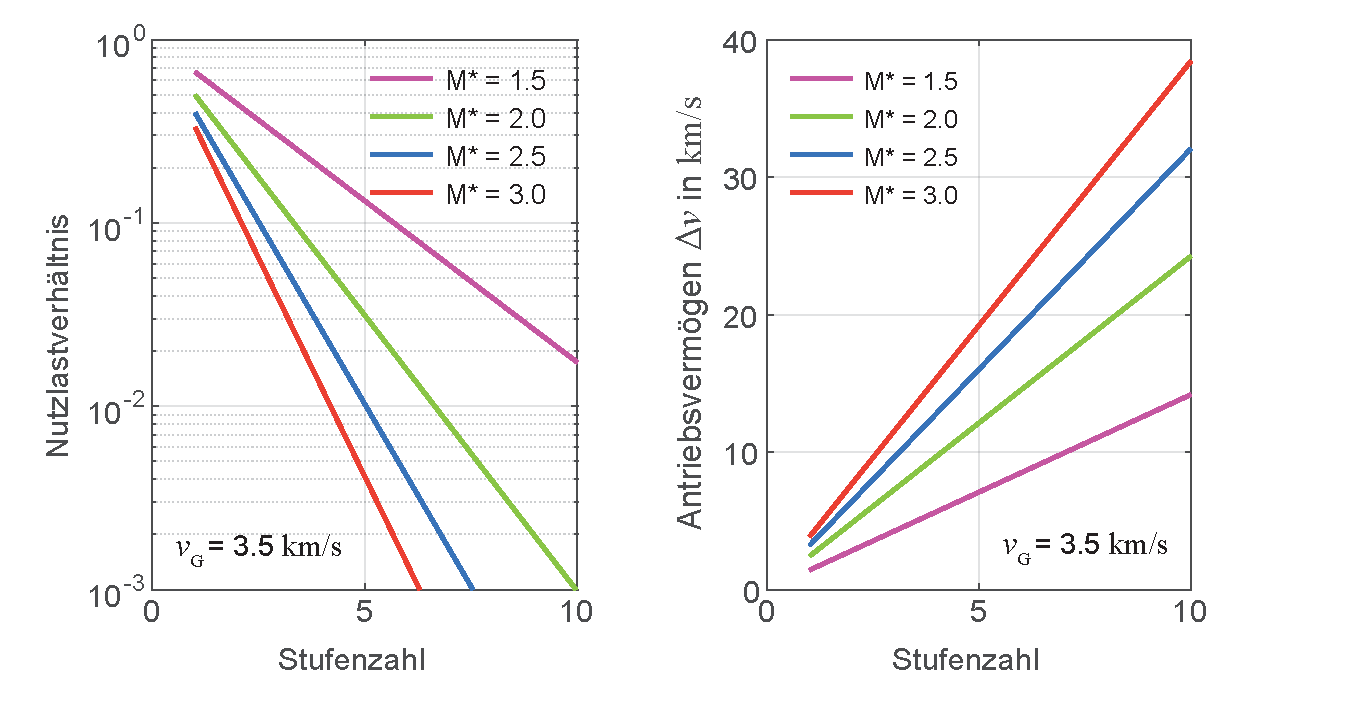
\includegraphics[width=\textwidth]{MehrStufenTheorie.pdf} 
	\caption[Nutzlastverh�ltnis �ber Antriebsbudget f�r mehrstufige Raketen.]{Nutzlastverh�ltnis �ber Antriebsbudget f�r mehrstufige Raketen bei gleichen $v_{\text{G},i}= v_\text{G}{}^*$ und 
	gleichen Struktur- und Treibstoffmassen aller Unterraketen ($\mathcal{M}^* = m_{0,i}/(m_{0,i}-m_{\text{T},i})$). Siehe \matlab{}-Datei
\mladynref{Raketenstart04.m}.}
	\label{abb:adyn_rocket_lsg05}
\end{figure}

\end{sol} 
\textcolor{blue} {$\rightarrow$ zur} \probref{adyn_rocketbasic}.\\
\noindent\rule[1ex]{\textwidth}{0.5pt}  \newpage  \clearpage

%-----------------------------------------------------------------------------------------------------------


\begin{sol}{prob:adyn_rocketopt1}\label{lsg:adyn_rocketopt1} %�bung3
\textbf{Optimierung Mehrstufenrakete (Tandemstufung)}\\
\begin{enumerate}
	\item \textit{\textbf{L�sungsansatz �ber Extremwertberechnung - Beispiel Saturn V Maximalleistung 100 t Nutzlast}}\\ 
Wir starten von der Raketen-Gleichung f�r die Tandemstufung \eqref{eq:adyn_rockets19} und fordern, dass f�r ein Nutzlastverh�ltnis
\begin{align}
    \Delta v = \sum\limits_{i_1}^N \Delta v_i = \sum\limits_{i_1}^N v_{\text{G},i}\,\ln\,\frac{1}{\sigma_i + \frac{\mu_{i+1}}{\mu_i}}\,.\label{eq:adyn_rocketsopt01} ~~~~ \rightarrow ~~~~ \text{max}
\end{align}
gelten soll. Die Bedingung f�r das Maximum lautet, wenn $\mu_\text{L}$ und alle $\sigma_i$ gegeben sind:
\begin{align}
    \frac{\d \Delta v\lk\mu_2,\mu_3,\ldots,\mu_N\rk}{\d \mu_i} = 0 ~~~~ \text{f�r} ~~~~i= 2,3,\ldots,N\,.\label{eq:adyn_rocketsopt02}
\end{align}
Daraus folgt sofort:
\begin{align}
    \frac{\d}{\d\mu_i}\,\lek -v_{\text{G},i-1}\,\ln\lk\sigma_{i-1} + \frac{\mu_i}{\mu_{i-1}}\rk- v_{\text{G},i}\,\lk\sigma_i + \frac{\mu_{i+1}}{\mu_i}\rk\rek= 0\,.\label{eq:adyn_rocketsopt03}
\end{align}
Wir f�hren  die Ableitung aus und erhalten $N-1$ Gleichungen in $\mu_i$ der Form: ($i=2,3,\ldots,N$)
\begin{align}
    \mu_i{}^2 = \frac{\lk v_{\text{G},i}-v_{\text{G},i-1}\rk\,\mu_{i+1}}{v_{\text{G},i-1}\,\sigma_i}\,\mu_i-\frac{v_{\text{G},i}}{v_{\text{G},i-1}}\,\frac{\sigma_{i-1}}{\sigma_i}\,\mu_{i-1}\,\mu_{i+1} = 0 \,,\label{eq:adyn_rocketsopt04}
\end{align}
\bzw aufgel�st nach
\begin{align}
    \mu_i = Q_i\,\mu_{i+1}+\sqrt{\lk Q_i\,\mu_{i+1}\rk^2 + P_i\,\mu_{i+1}\,\mu_{i-1}}\label{eq:adyn_rocketsopt05}
\end{align}
mit 
\begin{subequations}
\begin{align}
    Q_i = \frac{v_{\text{G},i}-v_{\text{G},i-1}}{2\,v_{\text{G},i-1}\,\sigma_i} \label{eq:adyn_rocketsopt06a}
\end{align}
und
\begin{align}
    P_i = \frac{v_{\text{G},i}\,\sigma_{i-1}}{v_{\text{G},i-1}\,\sigma_i}\;. \label{eq:adyn_rocketsopt06b}
\end{align}
\end{subequations}
F�r eine zweistufige Rakete ist $N=2$ und damit gibt es nur eine Bestimmungsgleichung f�r $\mu_2$ (da $\mu_1=1$ und $\mu_3 = \mu_L$):
\begin{align}
    \mu_2 = Q_2\,\mu_\text{L} + \sqrt{\lk Q_2\,\mu_\text{L}\rk^2 + P_2\,\mu_\text{L}}\,. \label{eq:adyn_rocketsopt07}
\end{align}
F�r eine dreistufige Rakete  ($N=3$) gibt es zwei Bestimmungsgleichungen
\begin{subequations}
\begin{align}
    \mu_2 &=  Q_2\,\mu_3 + \sqrt{\lk Q_2\,\mu_3\rk^2 + P_2\,\mu_3}\,, \label{eq:adyn_rocketsopt08a}\\
    \mu_3 &= Q_3\,\mu_\text{L} + \sqrt{\lk Q_3\,\mu_\text{L}\rk^2 + P_3\,\mu_\text{L}\,\mu_2}\,, \label{eq:adyn_rocketsopt08b}
\end{align}
\end{subequations}
die man am besten numerisch in \matlab{}  nach $\mu_2$ und $\mu_3$ l�st (siehe \mscr{} \mladynref{RaketenOptimierung01.m}). F�r $N=3$ f�hrt das Gleichungssystem 
nach einiger Algebra auf eine noch analytisch l�sbare kubische Gleichung f�r $\mu_3$, die wir hier angeben:
\begin{align*}
    \mu_3^3 - B\,\mu_3^2 + C\,\mu_3 - D &= 0 \\
		\text{mit}~~ B &= 2\mu_\text{L}\,(2Q_3+ Q_2\,P_3)\,,\\
		             C &= 4Q_3\,\mu\text{L}^2\,(Q_3+Q_2\,P_3)\,,\\
								 D &= P_2\,P_3{}^2\, \mu\text{L}^2\,.
\end{align*}
In \figref{adyn_optrockets01}a haben wir die Massenverh�ltnisse $\mu_2,\,\mu_3$ der einzelnen Raketenstufen f�r den Fall einer zweistufigen und einer dreistufigen Rakete �ber dem Nutzlastverh�ltnis aufgetragen. In \figref{adyn_optrockets01}b ist das mit heutigen Werten f�r $v_\text{G}$ maximal erzielbare Antriebsverm�gen f�r eine Stufenzahl von $N=2$ und $N=3$ �ber das Nutzlastverh�ltnis aufgetragen. Man erkennt daraus, dass man mit einer zweistufigen Rakete nicht zum Mond kommt, da $\Delta v$ kleiner als die 2.\,\gls{vkosmos} ist. \\

\begin{figure}[H]
	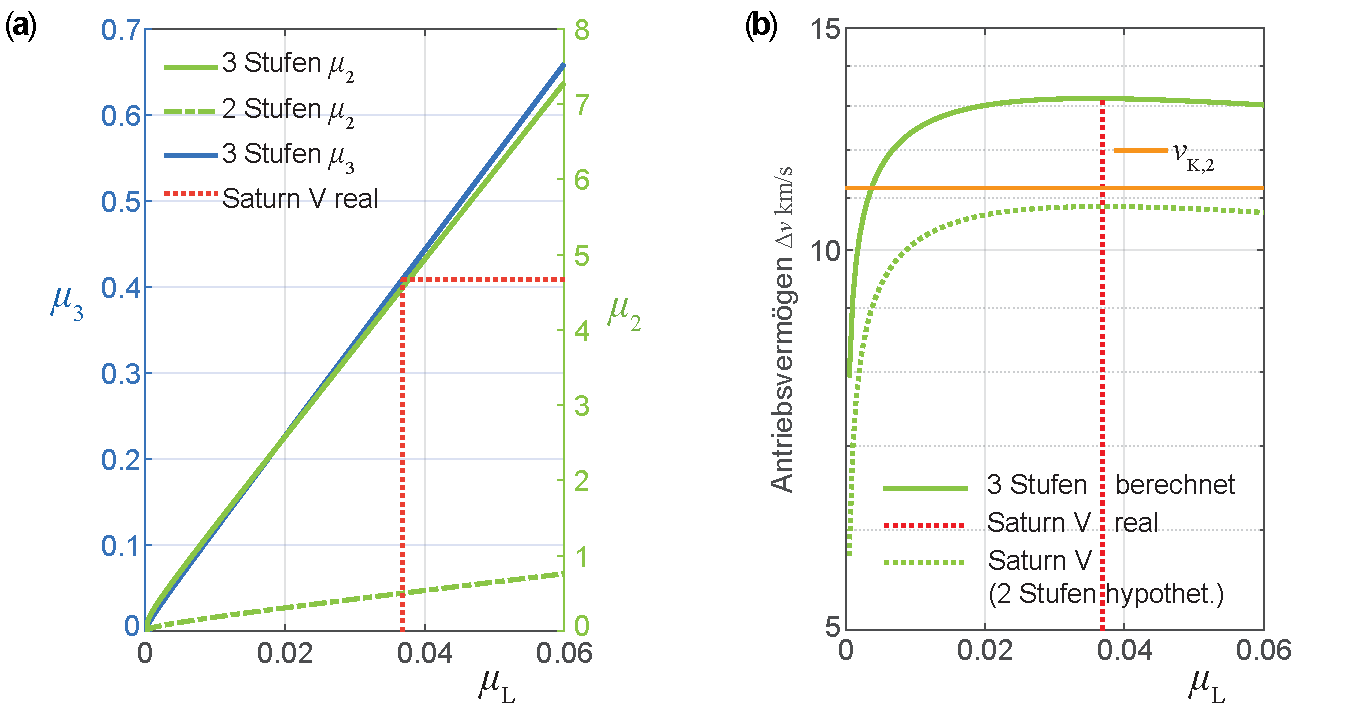
\includegraphics[width=\textwidth]{RaketenOptimierung01.pdf} 
	\caption[Optimierung einer Dreistufen-Rakete.]{Optimierung einer Dreistufen-Rakete. L�sung �ber Extremwertberechnung. \fa Berechnung der Massenverh�ltnisse der einzelnen Raketenstufen \fb Antriebsverm�gen f�r eine Dreistufen-Rakete (berechnet) und f�r die Saturn V. Zum Vergleich sind auch die Werte f�r eine (hypothetische) Ausf�hrung der Saturn V als Zweistufen-Rakete gezeigt.}
	\label{abb:adyn_optrockets01}
\end{figure}

\item \textit{\textbf{L�sungsansatz �ber Lagrange-Multiplikatoren - Beispiel Saturn V zum Mond}}\\ 
	
	Gegeben seien nach Aufgabenstellung: $v_{\text{G},i}$ (Ausstr�mgeschwindigkeit), $\sigma_i$ (Strukturparameter) und $m_0$ (Gesamtmasse der Rakete) \\
Variiert werden k�nnen die Massenverh�ltnisse $\mu_i$ oder, was gleichbedeutend ist, die Teil-Nutzlastverh�ltnisse $\eta_i$, die wir �ber
\begin{align}
    \eta_i = \frac{m_{\text{L},i}}{m_{0,i}-m_{0,i+1}} = \frac{m_{0,i+1}}{m_{\text{S},i} + m_{\text{T},i}} \label{adyn_optrocket11}
\end{align}
definieren. \\
Als $i$-tes Nutzlastverh�ltnis wird die Masse der n�chsten $\lk i+1\rk$-ten Unterrakete im Verh�ltnis zur Summe von Struktur- und Treibstoffmasse der $i$-ten Stufe definiert. Die Zahl der Stufen k�nnte ebenfalls variiert werden, soll aber hier festgehalten werden. \\
Zu optimieren/maximieren sind das Gesamt-Nutzlastverh�ltnis $\mu_\text{L}$ und das Gesamt-Antriebsverm�gen $\Delta v$, also max $\mu_\text{L}\lk \Delta v\rk$ \bzw max $\Delta v\lk\mu_\text{L}\rk $.\\
In Kapitel �ber den Lagrange-Formalismus im Band I hatten wir die Methode der Lagrange-Multiplikatoren kennen gelernt, mit der man die Extremwertberechnung der Wirkung $S$ bei Vorliegen von Zwangsbedingungen \bzw Nebenbedingungen durchf�hren konnte. Wir wenden dies f�r unser Problem an. Der Wirkung $S$ entspricht hier die Gr��e $\mu_\text{L}$ \bzw $\Delta v$, die Nebenbedingungen sind duch die $m_{\text{S},i}$ \bzw $\sigma_{i}$ gegeben und die "`Bewegungsgleichungen"' ergeben sich dann durch:
\begin{align}
    \frac{\d\lk\mu_\text{L}\rk}{\d \eta_j} + \lambda_{\mu_\text{L}}\,\frac{\d\lk \Delta v\rk}{\d \eta_j} = 0 ~~~~ \text{(maximieren von $\mu_\text{L}$)} \label{adyn_optrocket12}
\end{align}
\bzw
\begin{align}
    \frac{\d\lk\Delta v\rk}{\d \eta_j} + \lambda_{\Delta v}\,\frac{\d\lk \mu_\text{L}\rk}{\d \eta_j} = 0 ~~~~ \text{(maximieren von $\Delta v$)} \,.\label{adyn_optrocket13}
\end{align}
F�r $\lambda_{\mu_\text{L}} = 1/\lambda_{\Delta v}$ beschreiben beide Gleichungen das gleiche mathematische Problem.\\
Wir f�hren die Ableitungen aus und erhalten:
\begin{align}
\begin{split}
     \frac{\d\lk\Delta v\rk}{\d \eta_j} &= -v_{\text{G,j}}\,\frac{1-\sigma_j}{1+\eta_j}\,\frac{1}{\sigma_j+\eta_j} \,,\\
     \frac{\d\lk\mu_\text{L}\rk}{\d \eta_j}  &= \frac{\mu_\text{L}}{\eta_j\lk 1+\eta_j\rk}
\end{split}\label{adyn_optrocket14}
\end{align}
und erhalten aus \eqref{adyn_optrocket12}
\begin{align}
    \frac{\mu_\text{L}}{\eta_j\lk 1+\eta_j\rk} = \lambda_{\mu_\text{L}}\,v_{\text{G},j}\,\frac{1-\sigma_j}{1+\eta_j}\,\frac{1}{\sigma_j + \eta_j} \label{adyn_optrocket15} \,.
\end{align}
Daraus folgt sofort
\begin{align}
    v_{\text{G},j}\,\eta_j\,\frac{1-\sigma_j}{\sigma_j + \eta_j} = \frac{\mu_\text{L}}{\lambda_{\mu_\text{L}}} =:\gamma = \text{const} ~~~~ j=1,2,\ldots,N \,.\label{adyn_optrocket16}
\end{align}
Damit haben wir die Grundgleichungen f�r die Optimierung. \\
$\gamma$ ist noch eine unbekannte Gr��e, die es aus \eqref{adyn_optrocket16} zu bestimmen gilt. Wir nehmen diese zun�chst als bestimmt an, so dass sich dann die optimalen Nutzlastverh�ltnisse ergeben zu:
\begin{align}
    \eta_\text{j,\text{opt}} = \frac{\gamma\,\sigma_j}{\lk 1-\sigma_j\rk\,v_{\text{G},j}-\gamma}~~~~ j=1,2,\ldots,N \,.\label{adyn_optrocket17}
\end{align}
Wir setzen diese in die Raketen-Gleichung f�r die serielle Stufung \eqref{eq:adyn_rockets17} ein und erhalten:
\begin{align}
    \Delta v = \sum\limits_{j=1}^N\,v_{\text{G},j}\,\ln\,\frac{1+\eta_j}{\sigma_j + \eta_j} = \sum\limits_{j=1}^Nv_{\text{G},j}\,\ln\,\frac{v_{\text{G},j}-\gamma}{\sigma_j\,v_{\text{G},j}}\,.\label{adyn_optrocket18}
\end{align}
F�r das totale Nutzlastverh�ltnis 
\begin{align}
    \mu_\text{L} = \frac{m_\text{L}}{m_0} = \prod\limits_{j=1}^N\frac{\eta_j}{1+\eta_j} = \prod\limits_{j=1}^N \frac{\gamma\,\sigma_j}{\lk 1-\sigma_j\rk\lk v_{\text{G},j}-\gamma\rk}\,.\label{adyn_optrocket19}
\end{align}
Der weitere Weg besteht darin, dass man aus \eqref{adyn_optrocket18} f�r bekannte $\sigma_j$, $\Delta v$ die Konstante $\gamma$ (die aus dem Lagrange-Multiplikator abgeleitet wurde) bestimmt und diese in \eqref{adyn_optrocket19} einsetzt, um $\mu_\text{L,opt}$ zu erhalten. \\
Die Konstante $\gamma$ muss aus der Gleichung \eqref{adyn_optrocket16} numerisch bestimmt werden, was wir vorteilhaft in \matlab\,im Skript \mladynref{RaketenOptimierung02.m} ausgef�hrt haben.\\
Wenn wir die in der �bung in Tabelle \ref{tab:adyn_parameter_Apollo11} angegebenen Werte verwenden, erhalten wir aus der Rechnung einen Wert von $\mu_\text{L} = 0.0176$, der nur wenig von dem tats�chlichen (etwas kleineren) Wert von $\mu_\text{L} = 0.0162$ abweicht, mit dem die NASA (vermutlich aus Sicherheitsgr�nden) operierte.
In \figref{adyn_optrockets02} ist das maximale Nutzlastverh�ltnis gezeigt, mit der eine Nutzlast von $m_\text{L} = \mu_\text{L,opt}\cdot m_0$ auf ein bestimmtes Antriebsverm�gen gebracht werden kann.\\
Es sei noch darauf hingewiesen, dass $\gamma < \mathrm{min}\lk v_{\text{G},j}\,\lk 1-\sigma_j\rk \rk \,$f�r alle $j=1,\ldots,N$ sein muss, was bei der numerischen Berechnung zu ber�cksichtigen ist.
	
\begin{figure}[H]
	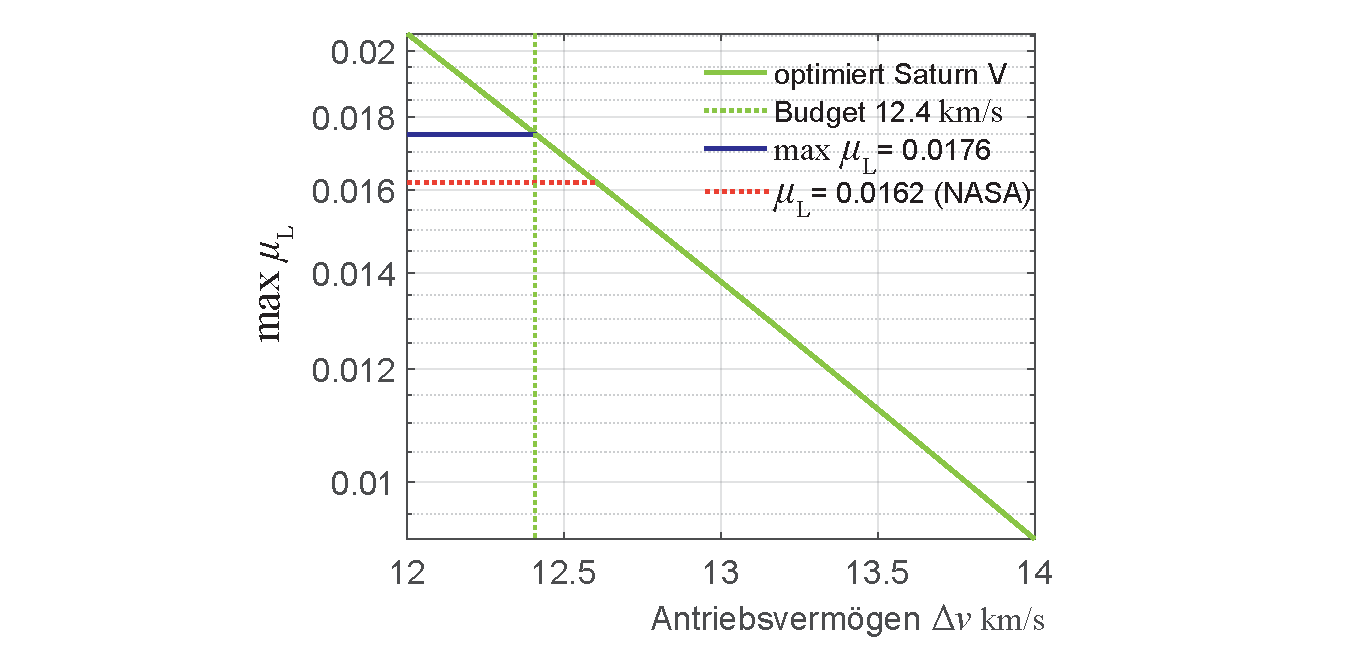
\includegraphics[width=\textwidth]{RaketenOptimierung02.pdf} 
	\caption[Optimierung einer Dreistufen-Rakete.]{Optimierung Saturn V Konfiguration f�r die Apollo Missionen. L�sung �ber Methode der Lagrange-Multiplikatoren. Berechnung des optimalen Antriebsverm�gens/Nutzlastverh�ltnisses.}
	\label{abb:adyn_optrockets02}
\end{figure}


\end{enumerate}

\end{sol} 
\textcolor{blue} {$\rightarrow$ zur} \probref{adyn_rocketopt1}.\\
\noindent\rule[1ex]{\textwidth}{0.5pt}  \newpage  \clearpage


%-----------------------------------------------------------------------------------------------------------


\begin{sol}{prob:adyn_rocketopt2}\label{lsg:adyn_rocketopt2} %�bung4
\textbf{Vergleich Mehrstufenrakete (Serielle und Parallelstufung)} \\ \\
Wir fassen die Vor- und Nachteile der Tandemstufung gegen�ber der Parallelstufung  in der folgenden Tabelle zusammen.\\
\begin{table}%tab1
\caption{Vor- und Nachteile der Tandemstufung gegen�ber der Parallelstufung.}
\smallskip
\hspace{1.5cm}
\begin{tabular}{L{3cm}L{3cm}L{3cm}}
\svhline\noalign{\smallskip}
Eigenschaft				    			& Tandemstufung				& Parallelstufung \\
\noalign{\smallskip}\svhline\noalign{\smallskip}
\noalign{\smallskip}
Startbeschleunigung							&kleiner &gr��er\\	
Strukturbelastung 							&kleiner &gr��er\\	
Biegemomente      							&gr��er  &kleiner\\	
Aerodynamische Verluste 				&kleiner &gr��er\\	
Gravitationsverluste						&gr��er  &kleiner\\	
Gesamtl�nge Rakete							&gr��er  &kleiner\\	
\noalign{\smallskip}
\svhline\noalign{\smallskip}
\end{tabular} \\
\label{tab:adyn_vergleich_staging}
\end{table}%tab1


\end{sol} 
\textcolor{blue} {$\rightarrow$ zur} \probref{adyn_rocketopt2}.\\
\noindent\rule[1ex]{\textwidth}{0.5pt}  \newpage  \clearpage


%-----------------------------------------------------------------------------------------------------------


%-----------------------------------------------------------------------------------------------------------
%-----------------------------------------------------------------------------------------------------------

\subsection{�bungen zu Umlaufbahnen}

\medskip

%-----------------------------------------------------------------------------------------------------------

\begin{sol}{prob:adyn_orbits1}\label{lsg:adyn_orbits1} %�bung5
\textbf{Bahnparameter aus Bodenbeobachtungen}\\ \\
\textit{Bahnparameter von Satelliten mit gegebenen geozentrischen Orts- und Geschwindigkeitsdaten:}\\ \\
Wir verwenden die Formeln aus \kap{adyn_orbits_determination_rv} und erhalten:\\

Satellit 1 (HEO)
\begin{align*}
	&\text{Halbachse}\,\,a & \SI{20251.57}{\km}\\
	&\text{Exzentrizit�t}\,\,e & 0.777596\\
	&\text{Bahnneigung} \,\,i &   10.194 \degree\\
	&\text{Knoten} \,\, \Omega &  171.951 \degree\\
	&\text{Arg. Perig�um} \,\, \omega &  86.081 \degree\\
	&\text{Mittl. Anomalie} \,\, M &  138.824  \degree\\
	&\text{Mittl. Bewegung} \,\, n & \SI{2.19e-04}{\per\second} \\
\end{align*}

Satellit 2 (LEO)
\begin{align*}
	&\text{Halbachse}\,\,a & \SI{8225.40}{\km}\\
	&\text{Exzentrizit�t}\,\,e & 0.076722\\
	&\text{Bahnneigung} \,\,i &   6.707 \degree\\
	&\text{Knoten} \,\, \Omega &  145.881 \degree\\
	&\text{Arg. Perig�um} \,\, \omega &  86.476 \degree\\
	&\text{Mittl. Anomalie} \,\, M &  167.278  \degree\\
	&\text{Mittl. Bewegung} \,\, n & \SI{8.46e-04}{\per\second}
\end{align*}

\newpage

\textit{Bahnparameter der ISS aus den ver�ffentlichten geozentrischen Orts- und Geschwindigkeitsdaten der NASA:}\\
	%\url{https://spotthestation.nasa.gov/trajectory_data.cfm}\\

Auch hier verwenden wir die Formeln aus \kap{adyn_orbits_determination_rv} und erhalten:
\begin{align*}
	&\text{Halbachse}\,\,a & \SI{6803.28}{\km}\\
	&\text{Bahnh�he}\,\,h & \SI{425.28}{\km}\\
	&\text{Exzentrizit�t}\,\,e & 0.001855\\
	&\text{Bahnneigung} \,\,i &  51.751 \degree\\
	&\text{Knoten} \,\, \Omega &  47.685 \degree\\
	&\text{Arg. Perig�um} \,\, \omega & 124.00 \degree\\
	&\text{Mittl. Anomalie} \,\, M & 315.75 \degree\\
	&\text{Umlaufzeit} \,\, n & \SI{93.8 }{\minute}
\end{align*}
Die mittlere Anomalie $M$ wurde so angepasst, dass der Anfangswert mit den NASA Daten �bereinstimmt. Wir verweisen auf \kap{adyn_orbits_determination_singulaer}
zur Berechnung alternativer Bahnparameter bei kreisf�rmigen und �quatorialen Bahnen, sowie auf die Zusatzaufgabe \probref{adyn_orbits_zusatz1}.
\begin{figure}[H]
	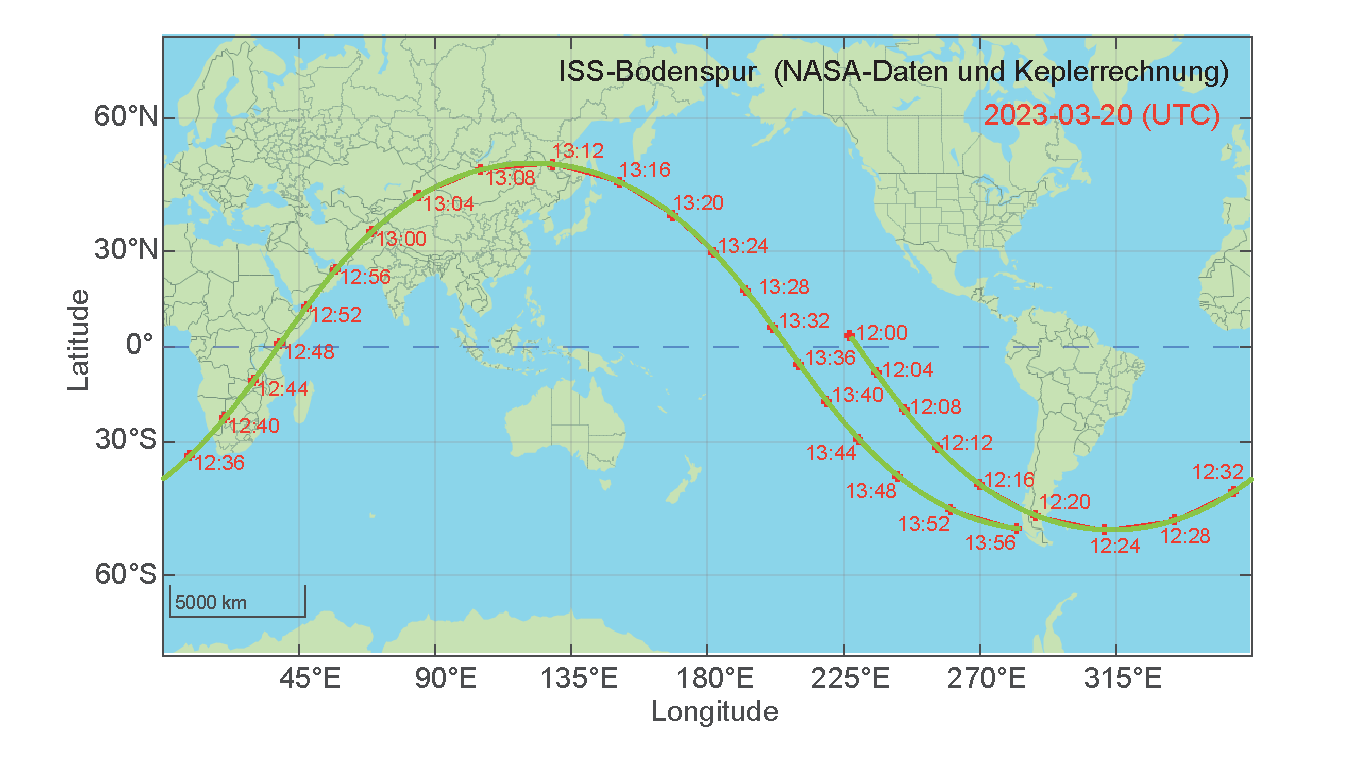
\includegraphics[width=\textwidth]{GroundTrackISS20032023.pdf} 
	\caption[Bodenspur der ISS.]{Bodenspur der ISS. Vergleich NASA Daten und Berechnung Keplerbahn.}
	\label{abb:adyn_satobserv02}
\end{figure}
Die Berechnungen finden sich im Detail im \mscr{} \mladynref{BahnparaBestimmung01.m}. 

\end{sol} 
\textcolor{blue} {$\rightarrow$ zur} \probref{adyn_orbits1}.\\
\noindent\rule[1ex]{\textwidth}{0.5pt}  \newpage  \clearpage

%-----------------------------------------------------------------------------------------------------------
\newpage

\begin{sol}{prob:adyn_orbits2}\label{lsg:adyn_orbits2} %�bung6
\textbf{Bodenspuren von Erdsatelliten}\\ 

\begin{itemize}
	\item \textit{\textbf{Bodenspuren verschiedener Satellitenarten}}\\
		\begin{itemize}
			\item Bodenspur eines GEO-Satelliten.
			\item Bodenspur eines Molnija-Satelliten (HEO-Satelliten).
			\item Bodenspur eines polaren Satelliten. 
		\end{itemize}
		\begin{figure}[H]
			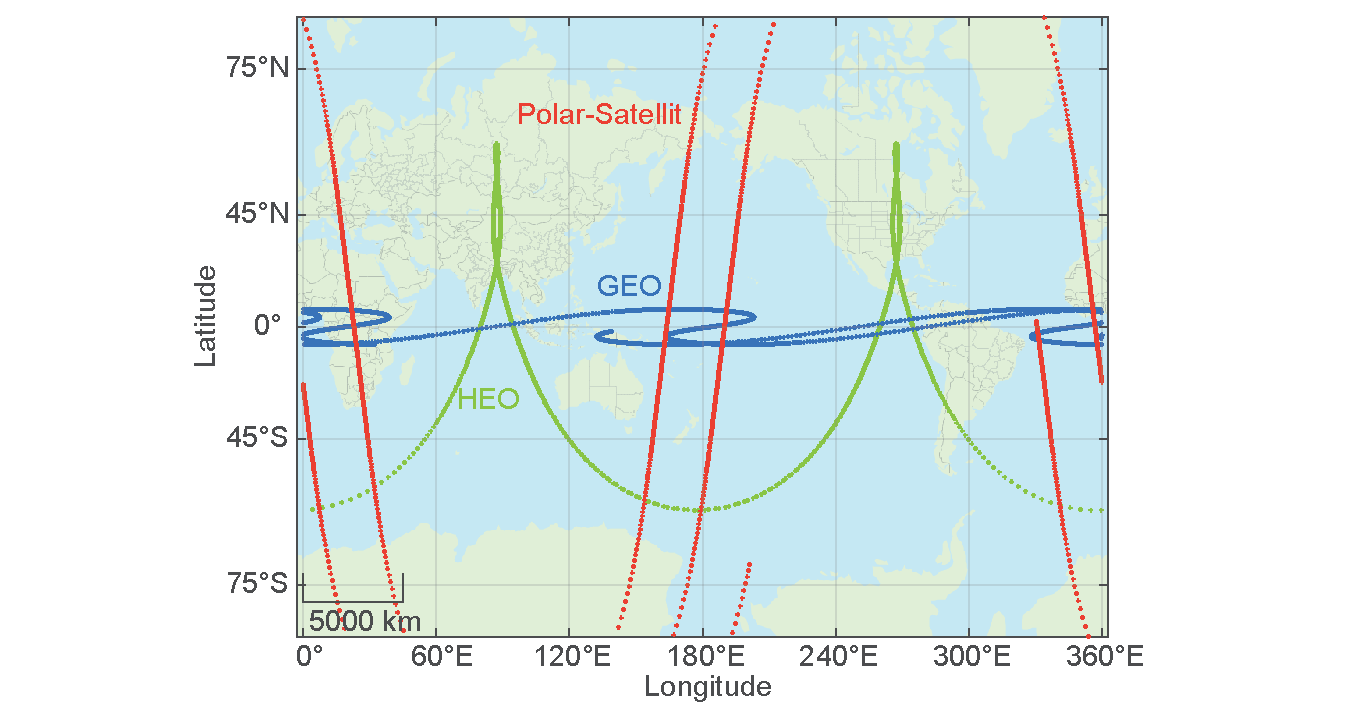
\includegraphics[width=0.9\textwidth]{Orbits03a.pdf} 
			\caption[Bodenspuren von verschiedenen Satelliten.]{Bodenspuren von verschiedenen Satelliten. GEO:\, $a = \SI{25000}{\km},\, e = 0.73,\, i = 8\degree,\, \Omega =45\degree$,\,\, HEO (Typ Molnija-Satelliten):\, $a = \SI{26555}{\km},\, e = 0.72,\, i = 63.4\degree,\, \Omega =120\degree,\,\omega =270\degree$,\,\, Polar-Satellit:\, $a = \SI{7330}{\km},\, e = 0.0,\, i = 93\degree,\, \Omega =130\degree,\,\omega =0\degree$.}
			\label{abb:adyn_orbits03a}
			\end{figure}
	\item \textit{\textbf{Bodenspuren verschiedener Satelliten in geosynchronen Umlaufbahnen}}\\

				Die Bodenspuren \figref{adyn_orbits03b} �hneln den verschiedenen Analemma, die wir im \kap{kulmination_sonne} \bzw in der \probref{hm_Analemma_Mars} kennen gelernt hatten. Das ist nicht verwunderlich. In einer geozentrischen Betrachtung �bernehmen die Satelliten die Rolle der Sonne, die unterschiedlichen Formen des \textit{\anf{Satelliten-Analemmas}} kommen durch die unterschiedlichen Bahnparameter zustande. Siehe auch im Detail \probref{hm_Analemma_Mars}.\\
\newpage
			\begin{figure}[H]
			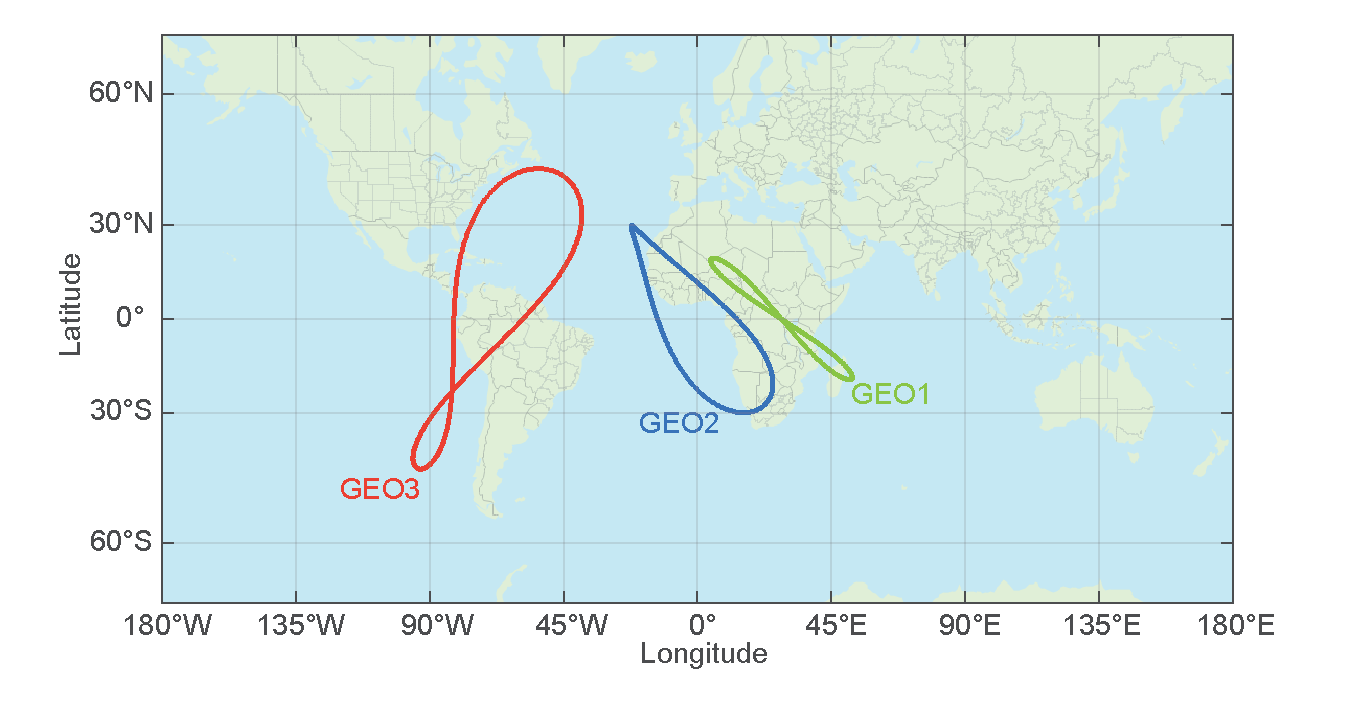
\includegraphics[width=0.95\textwidth]{Orbits03b.pdf} 
			\caption[Bodenspuren von verschiedenen geosynchronen Satelliten.]{Bodenspuren von verschiedenen geosynchronen Satelliten. Parameter siehe \probref{adyn_orbits2}.}
			\label{abb:adyn_orbits03b}
			\end{figure}
\item \textit{\textbf{Bodenspur ISS}}\\
			\begin{figure}[H]
			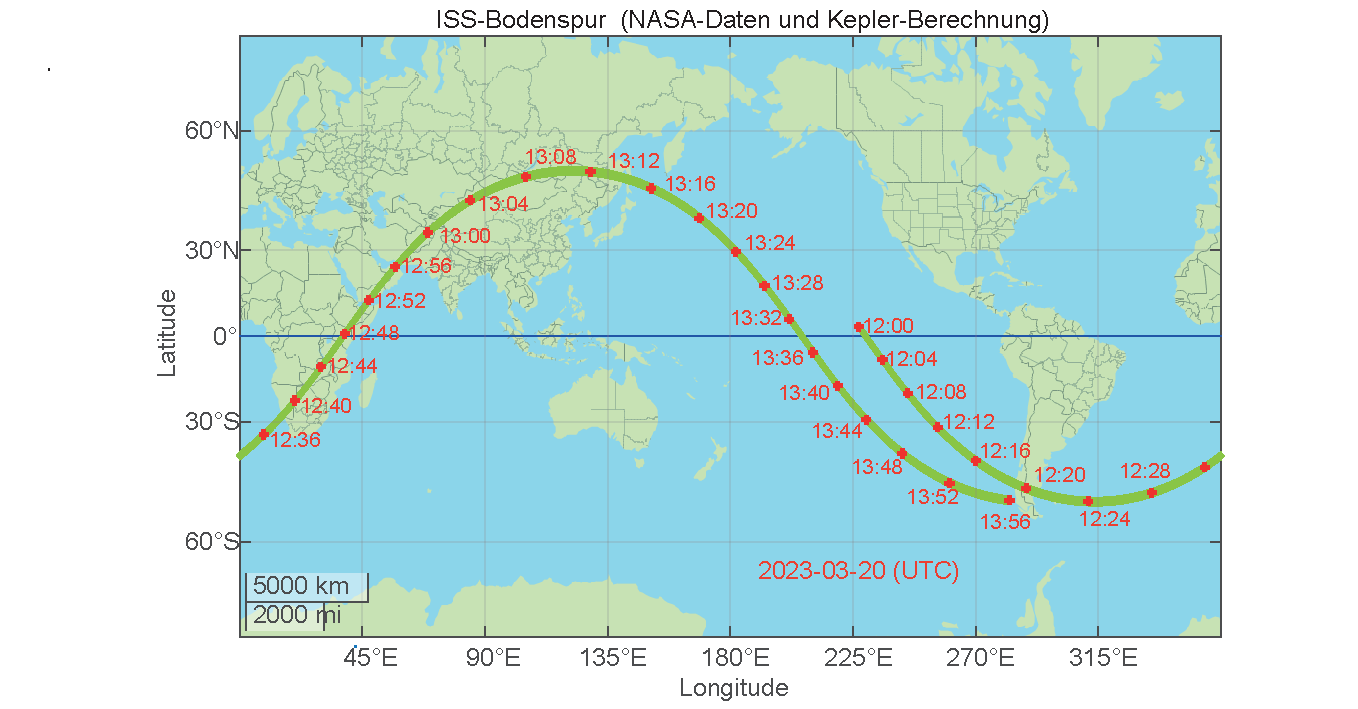
\includegraphics[width=0.95\textwidth]{ISSBodenspur.pdf} 
			\caption[Bodenspuren der ISS.]{Bodenspuren der ISS vom 20.03.2023. Parameter siehe \probref{adyn_orbits2}.}
			\label{abb:adyn_orbits03c}
			\end{figure}
\end{itemize}
Die Berechnungen finden sich im Detail im \mscr~\mladynref{SatPositionen01.m} \bzw \mladynref{SatPositionen02.m}.

\end{sol} 
\textcolor{blue} {$\rightarrow$ zur} \probref{adyn_orbits2}.\\
\noindent\rule[1ex]{\textwidth}{0.5pt}  \newpage  \clearpage

%-----------------------------------------------------------------------------------------------------------

\begin{sol}{prob:adyn_orbits3}\label{lsg:adyn_orbits3} %�bung7
\textbf{Bodenbeobachtung von Erdsatelliten}\\ \\

Die Berechnungen finden sich im Detail im \mscr~\mladynref{SatPositionen03.m} \bzw \mladynref{SatPositionen04.m}.
\begin{figure}[H]
	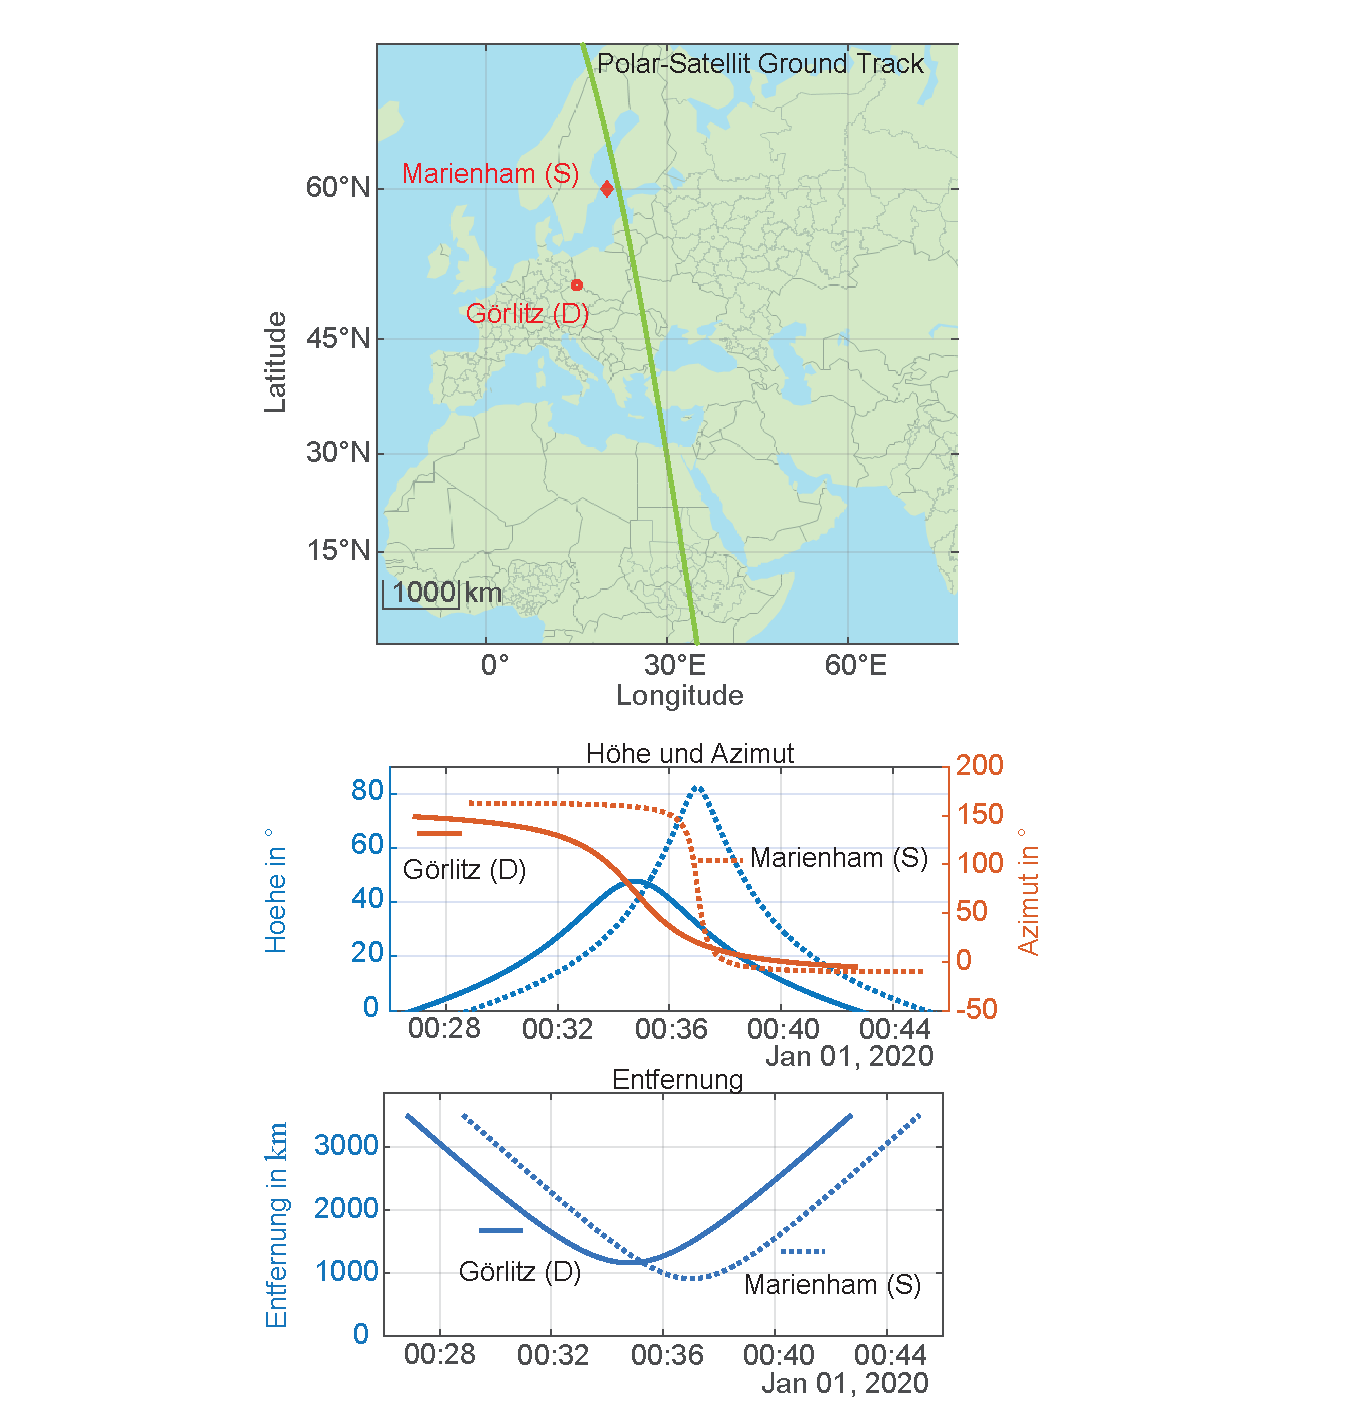
\includegraphics[width=\textwidth]{TopographPolarerSat.pdf} 
	\caption[Topographische Beobachtung eines polaren Satelliten.]{Bodenspur, Azimut, H�he und Entfernung eines polaren Satelliten von zwei Bodenstationen. Parameter siehe \probref{adyn_orbits3} und \mscr~\mladynref{SatPositionen03.m} \bzw \mscr~\mladynref{SatPositionen03a.m}.}
	\label{abb:adyn_satobserv03}
\end{figure}
\begin{figure}[H]
	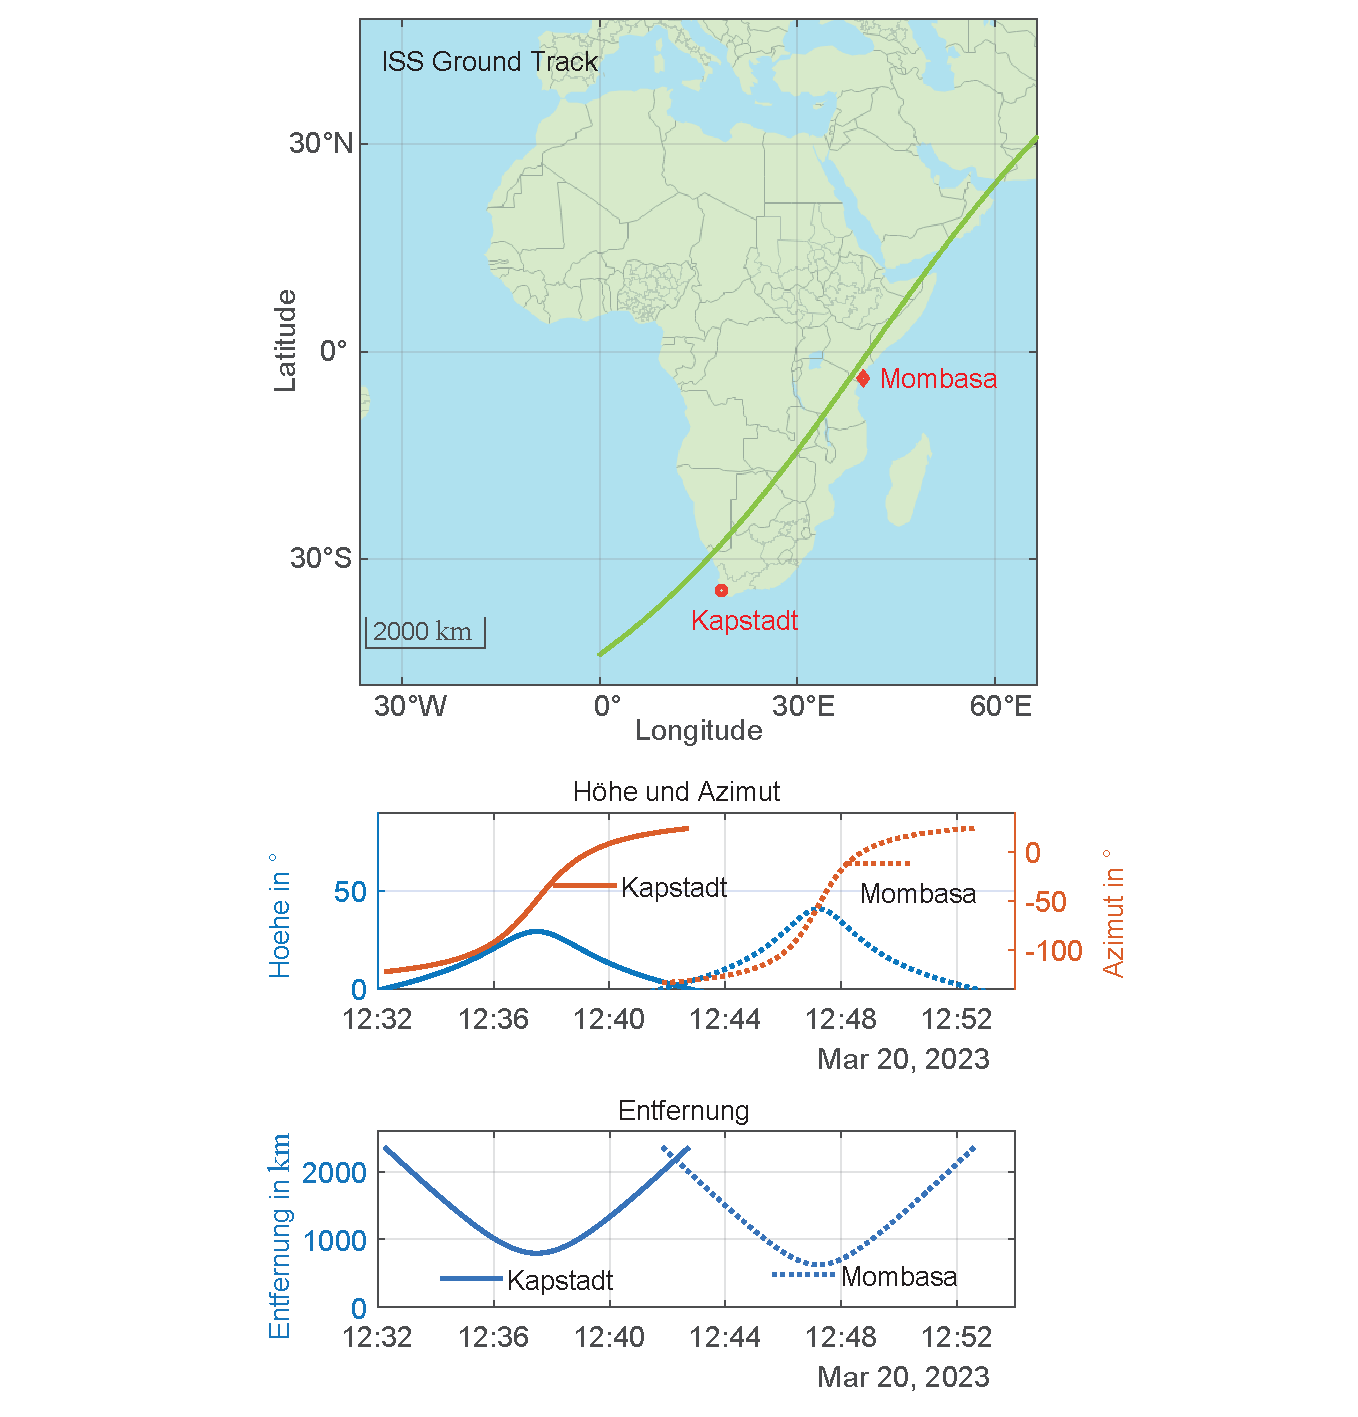
\includegraphics[width=\textwidth]{TopographISS.pdf} 
	\caption[Topographische Beobachtung der ISS.]{Bodenspur, Azimut, H�he und Entfernung der von zwei Bodenstationen. Parameter siehe \probref{adyn_orbits3} und \mscr~\mladynref{SatPositionen04.m}.}
	\label{abb:adyn_satobserv04}
\end{figure}

\end{sol} 
\textcolor{blue} {$\rightarrow$ zur} \probref{adyn_orbits3}.\\
\noindent\rule[1ex]{\textwidth}{0.5pt}  \newpage  \clearpage

%-----------------------------------------------------------------------------------------------------------

\begin{sol}{prob:adyn_orbits4}\label{lsg:adyn_orbits4} %�bung8
\textbf{Bodenbeobachtung eines Molniya-Satelliten}\\ \\

Die Berechnungen finden sich im Detail im \mscr~\mladynref{SatPositionen05.m}.
\begin{figure}[H]
	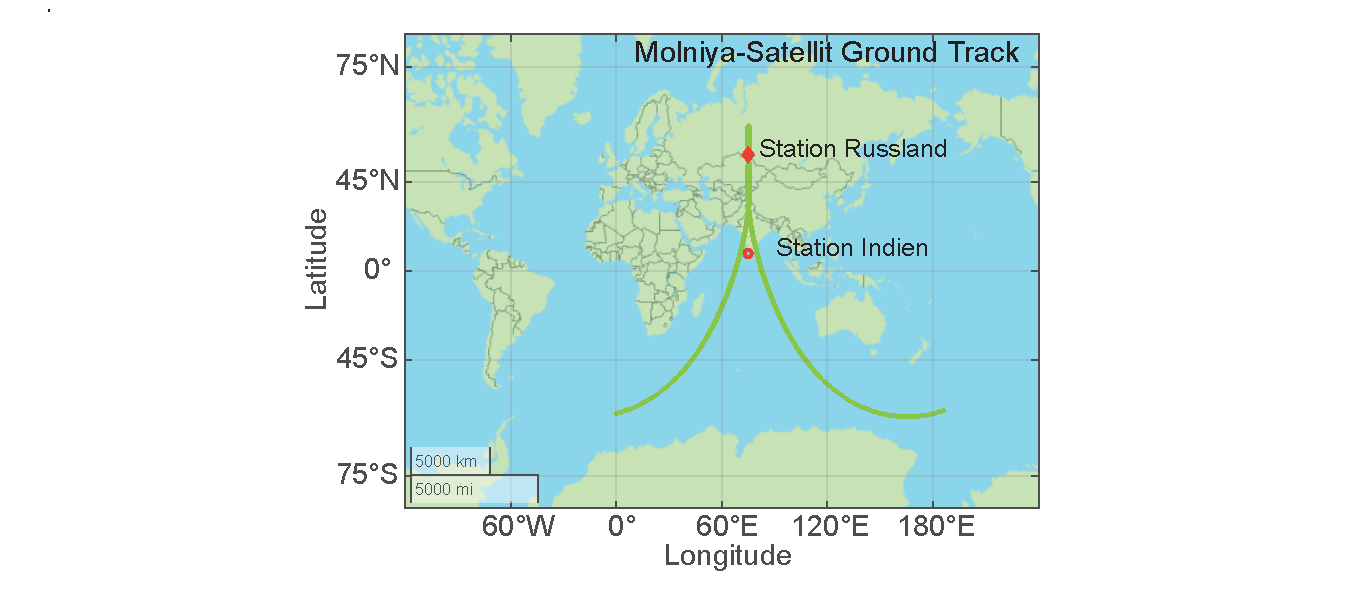
\includegraphics[width=\textwidth]{TopographMolniyaSat01.pdf} 
	\caption[Bodenspur eines Molniya-Satelliten.]{Bodenspur eines Molniya-Satelliten.\\Parameter siehe \probref{adyn_orbits4} und \mscr~\mladynref{SatPositionen05.m}.}
	\label{abb:adyn_MolniyaObserv01}
\end{figure}
\begin{figure}[H]
	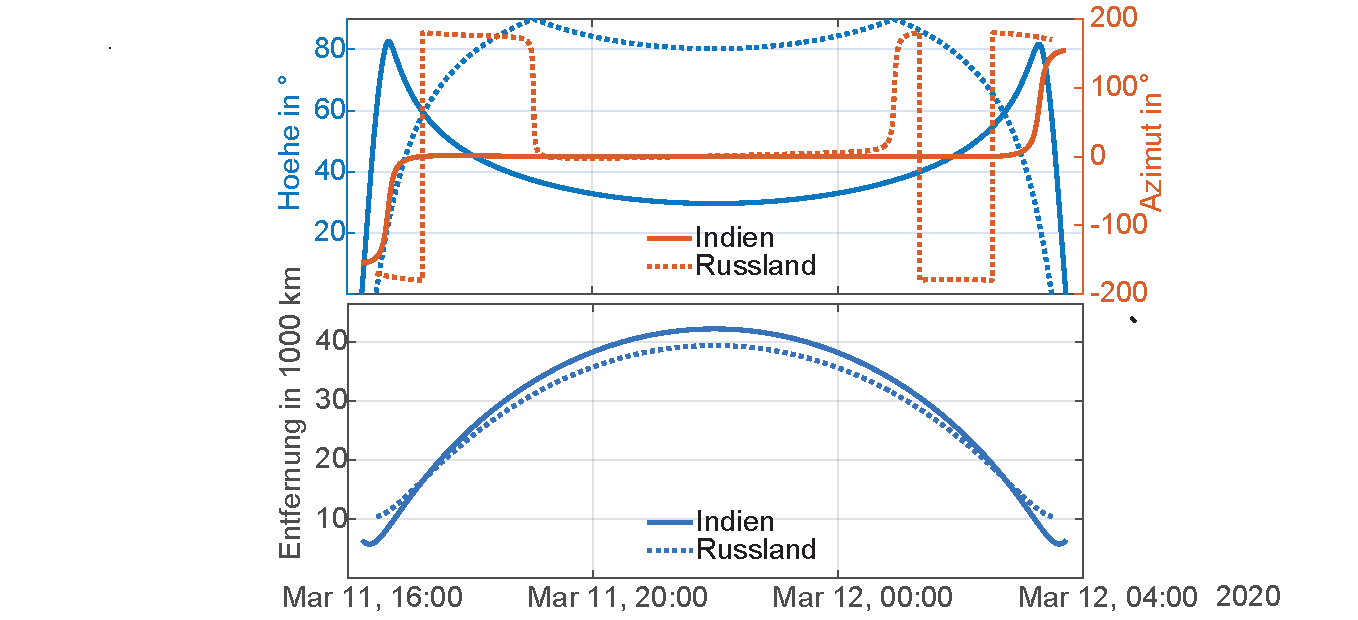
\includegraphics[width=\textwidth]{TopographMolniyaSat02.pdf} 
	\caption[Topographische Beobachtung eines Molniya-Satelliten.]{Azimut, H�he und Entfernung eines Molniya-Satelliten von zwei Bodenstationen. Parameter siehe \probref{adyn_orbits4} und \mscr~\mladynref{SatPositionen05.m}.}
	\label{abb:adyn_MolniyaObserv02}
\end{figure}
\end{sol} 
\textcolor{blue} {$\rightarrow$ zur} \probref{adyn_orbits4}.\\
\noindent\rule[1ex]{\textwidth}{0.5pt}  \newpage  \clearpage


%-----------------------------------------------------------------------------------------------------------

\begin{sol}{prob:adyn_orbits5}\label{lsg:adyn_orbits5} %�bung9
\textbf{Sonnensynchrone Bahnen}\\ \\

Die Drehimpulserhaltung gilt streng nur f�r das Zweik�rperproblem, dann ist auch die Bahnebene fest im Raum orientiert und die Bahn geschlossen.\\
Wie wir \zb in \kap{Periheldrehung} gesehen haben, bewirkt die Abplattung der Erde jedoch ein Drehmoment auf die Bahn und f�hrt zu einer Verschiebung der Rektaszension des aufsteigenden Knotens. 
Man kann mit Hilfe der St�rungsrechnung zeigen (siehe auch \probref{adyn_pertubations}), dass die Frequenz dieser Pr�zession des aufsteigenden Knoten sich nach folgender Formel berechnet:
	\begin{align}
		\dot{\Omega} = -\frac{3}{2} J_2\, \frac{2\pi}{T_\text{E}} \lk \frac{R_\text{E}}{a\,(1-e^2)} \rk^2 \cos i = 
		-\frac{3}{2} J_2\,R_\text{E}\, \sqrt{\frac{a_\text{E}}{a_\text{E}{}^2}} \, \frac{\cos i}{a^2\,(1-e^2)^2} = C\,f(a,e,i)\,. \label{eq:adyn_orbits5_01}
	\end{align}
Hierin sind $J_2$ die sogenannte zonale Harmonische\index{Harmonische!zonale} (siehe \kap{adyn_gravity_pertubations}) als Ma� f�r die Abplattung der Erde, $R_\text{E}$ der mittlere Erdradius, $a$ die gro�e Halbachse der Satellitenbahn und $i$ \bzw $e$ deren Neigung (Inklination) \bzw Exzentrizit�t. $T_\text{E} = 2\pi\sqrt{a_\text{E}{}^3/\mu_\text{E}}$ ist die Umlaufzeit der Erde um die Sonne.\footnote{Genauer gesagt ist es die Zeit eines anomalistischen Jahres ($\SI{365.25963}{}\,\mathrm{d}$, siehe \kap{hm_zeitdefinition})} Die Pr�zession ist umso gr��er, je geringer die Inklination $i$ und die Bahnh�he $a$ sind.\\
Wegen des Minuszeichen wirkt bei einer retrograden Bahnen (Bahn entgegen der Erdrotation, \dh $i > 90\degree$) diese Pr�zession in die gleiche Richtung wie die Erdrotation. Man kann also durch geeigneter Wahl von Inklination und Flugh�hen daf�r sorgen, dass sich die Bahn gerade um so viel verschiebt wie der mittleren Bewegung der Erde ($2\pi/T_\text{E}$) um die Sonne entspricht (\figref{adyn_synchron_orbit}). 

Bei einem SSO erfolgt der �berflug des Satelliten �ber einen Punkt auf der Oberfl�che des Planeten immer zur selben Ortszeit, vorausgesetzt die geographische Breite des Ortes liegt innerhalb des Bereiches, der durch die Inklination der Bahn begrenzt wird. Aufgrund dieser konstanten �berflugszeit lassen sich Beobachtungen von verschiedenen Tagen und Jahreszeiten gut miteinander vergleichen, deswegen haben ja Wetter- und Erdbeobachtungssatelliten oft solche Bahnen.

\begin{figure}[H]
	\includegraphics[width=\textwidth]{SonnensynchroneBahn.pdf} 
	\caption[Sonnensynchrone Bahn.]{Sonnensynchrone Bahn. Symbolische und nicht-ma�stabsgetreue Darstellung. }
	\label{abb:adyn_synchron_orbit}
\end{figure}

\newpage
\textbf{Zusatzaufgabe}\\

Wir wollen nun noch die Bodenspur des ERS-1 SSO-Satelliten berechnen \cite{Gottschalk1991}. Man k�nnte nun aus \eqref{eq:adyn_orbits5_01} einen der Parameter $a,\, e$ oder $i$ berechnen und die anderen vorgeben. 
Man hat aber eben mit $a$ einen weiteren Freiheitsgrad neben $i$, womit man auch fordern kann, dass die Bahnh�he $h$ so gew�hlt wird, dass ein �berflug �ber eine Gebiet (\zb das �berkreuzen des �quators nach $K$ Tagen \bzw. $N$ Orbits genau wiederholt (sogenannte \textit{Sonnensynchrone Repeat Orbits}).  Anfangs w�hlte man f�r den ERS-1 K=3, N=43, sp�ter ging man auf K=35.
Um das zu erreichen, muss man auch die St�rungen der Perihelverschiebung (siehe \kap{Stoerpotential_Merkur}) und der mittleren Anomalie ber�cksichtigen. Diese sind f�r kreisf�rmige Bahnen gegeben durch \cite{Montenbruck2012, Murray2008, Vallado2007}:

	\begin{align}
	\begin{split}
		\dot{\omega} = -\frac{3}{4} J_2\, n_0 \frac{R_\text{E}{}^2}{a^2} \lk 1 - 5\cos^2 i\rk \\ 
    \Delta n = n - n0  = -\frac{3}{4} J_2\, n_0 \frac{R_\text{E}{}^2}{a^2} \lk 1 - 2\cos^2 i\rk\,,
	\end{split}\label{eq:adyn_orbits5_02}
\end{align}

worin $n_0=\sqrt{(GM_\text{E}/a^3)}$ die mittlere Bewegung der Kepler-Bahn ist.
F�r sonnensynchrone Bahnen ist dann gefordert, dass gilt:

	\begin{align}
		\dot{\Omega} - \dot{\theta} = -360\degree\,, \\ 
\label{eq:adyn_orbits5_03}
\end{align}

woraus man f�r die Umlaufzeit einer solchen Bahn die Beziehung

	\begin{align}
		T_\text{P,SSO} = \frac{2\pi}{n_0-\Delta n-\dot{\omega}}\,, \\ 
\label{eq:adyn_orbits5_04}
\end{align}

was etwas l�nger ist als die Umlaufzeit im reinen Kepler-Fall.
Durch Iteration mit dem Startwert $T_\text{P,SSO}^{(0)}= 2\pi/n_0$ findet man �ber \eqref{eq:adyn_orbits5_02} aus \eqref{eq:adyn_orbits5_01} nacheinander $a$ und $i$ f�r die geforderten Bedingungen.\\

Wir finden:
\begin{align} 
  h &= a - R_\text{E} = \SI{7153.1}{\km} - \SI{6371.0}{\km} = \SI{782.1}{\km}\,, \\
	i &= 98.5\degree,
\end{align}
was f�r unsere Kreisbahnn�herung gut mit den Werten in \cite{Gottschalk1991} �bereinstimmt.
F�r die Berechnung der Bodenspur zu verschiedenen Zeiten, m�ssen Sie die Zeitabh�ngigkeit von $\Omega(t) = \Omega(t_0) + \dot{\Omega}\,(t-t_0)$ beachten.\\
Die Rechnungen finden sich im Detail im \mscr~\mladynref{SonnenSynchroneBahn.m} und ein Ergebnis in \figref{adyn_synchron_groundtrack}.

\begin{figure}[H]
	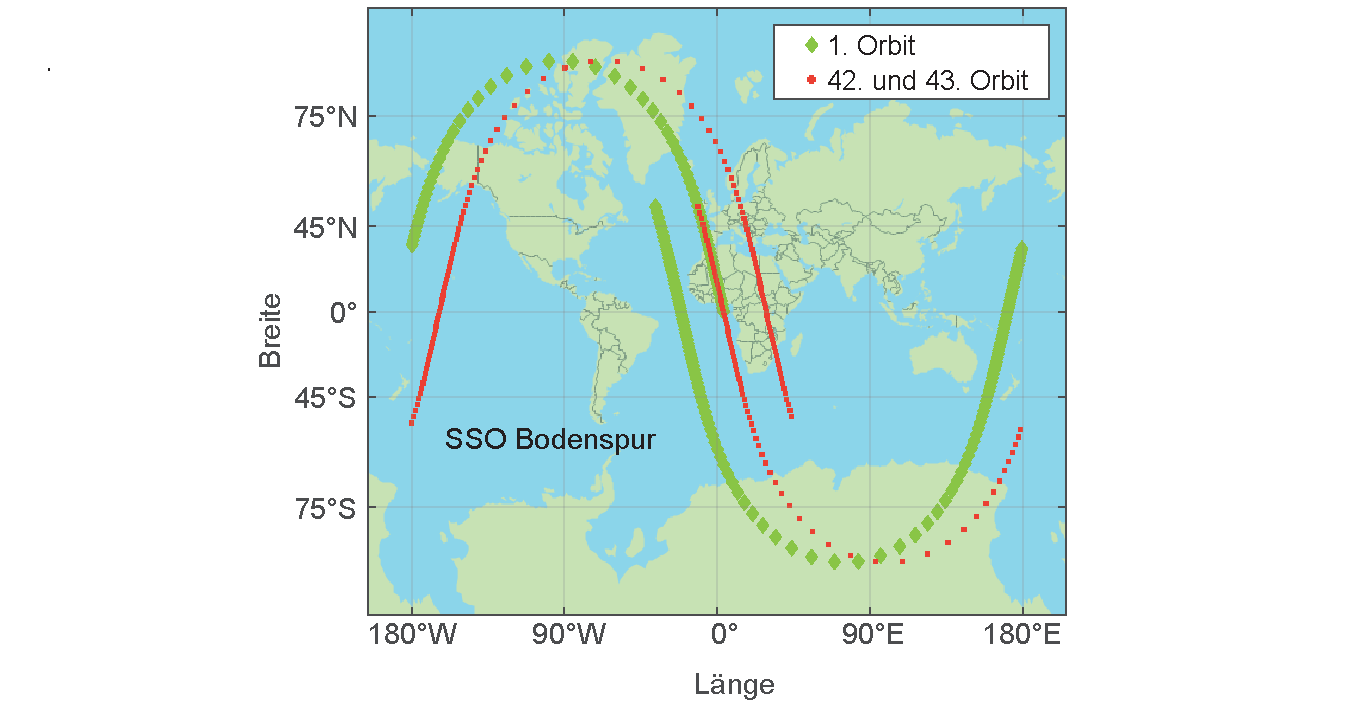
\includegraphics[width=\textwidth]{SonnensynchroneBodenspur.pdf} 
	\caption[Sonnensynchroner \textit{Repeat Orbit} -Bodenspur.]{Sonnensynchroner \textit{Repeat Orbit} - Bodenspur. Gezeigt sind Orbit Nr. 1 (willk�rlich gew�hlt) und die Orbits Nr 42 und Nr. 43 als Bodenspur. Man sieht, dass bei $N=43$ nach 3 Tagen der Satellit genau �ber die gleichen Gebiete fliegt wie beim Orbit $N=1$.}
	\label{abb:adyn_synchron_groundtrack}
\end{figure}

Wir empfehlen auch die Zusatz�bung \probref{adyn_pertubations}.

\end{sol} 
\textcolor{blue} {$\rightarrow$ zur} \probref{adyn_orbits5}.\\
\noindent\rule[1ex]{\textwidth}{0.5pt}  \newpage  \clearpage


%-----------------------------------------------------------------------------------------------------------

\begin{sol}{prob:adyn_starlink}\label{lsg:adyn_starlink} %�bung10
\textbf{Starlink}
\begin{figure}[H]
	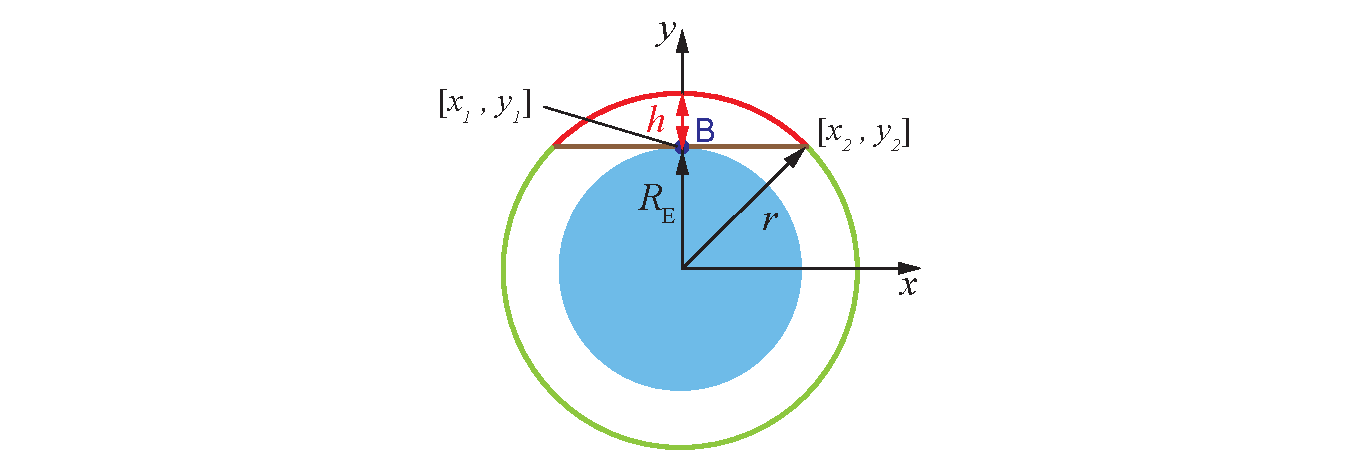
\includegraphics[width=\textwidth]{StarlinkGeometrie.pdf} 
	\caption[Zur Geometrie der Starlink-Beobachtungen.]{[Zur Geometrie der Starlink-Beobachtungen. Mit rot ist die Kugelkappe dargestellt die ein Beobachter auf der Erde sieht, wenn sich ein Starlink-Satellit in einer Kugelschale mit Radius $R_\text{E} + h$ bewegt.}
	\label{abb:adyn_starlink_ueb01}
\end{figure}
\begin{enumerate}
\item [1)] Wir berechnen zun�chst den Anteil $\gamma\lk h\rk$ der Kugelschale mit Radius $R_\text{E} + h$, den ein Beobachter von der Erdoberfl�che aus sieht. \\
    Nach \figref{adyn_starlink_ueb01} ist das:
    \begin{align*}
        \gamma\lk h\rk = \frac{A_\text{KK}}{A_\text{K}} \,. 
    \end{align*}
    Hierin ist $A_\text{K}$ ist die Oberfl�che einer Kugel $4\pi\,r^2 = 4\pi\,\lk R_\text{E} +h\rk^2$ und $A_\text{KK}$ die Oberfl�che der Kugelkappe, die man sich leicht �ber 
    \begin{align*}
       A_\text{KK} &= 2\pi\,r\int\limits_{x_1}^{x_2} y(x)\,\sqrt{1+y'(x){}^2}\D x = 2\pi\int\limits_{\rho_1}^{\rho_2} y(\rho)\,\sqrt{1+y'(\rho){}^2}\,\D \rho 
    \end{align*}
    mit $y = \sqrt{r^2-x^2}$,\,  $1+y'{}^2 = r^2/(r^2-x^2)$,\, $r = R_\text{E} + h$\, und \,$x= \rho\,\cos\phi$ herleiten kann.\\
		Somit erh�lt man 
    \begin{align}
		  A_\text{KK} &= 2\pi\,r \int\limits_{R_\text{E}}^{R_\text{E} + h}\,\D \rho = 2\pi\,\lk R_\text{E} +h\rk \,h \nonumber \\
      \rightarrow~~~  \gamma\lk h\rk &= \frac{2\pi\,\killA{\lk R_\text{E} + h\rk}\,h}{4\pi\,\lk R_\text{E} + h\rk^\killA{2}} = \frac{1}{2}\,\frac{h}{R_\text{E} + h} \,. \label{eq:adyn_starlink_ueb01}
    \end{align}
    Mit den Angaben aus der Aufgabenstellung sind damit jederzeit pro Schale $n_i $ Satelliten 
    \begin{align*}
        n_i = \gamma\lk n_i\rk \cdot \,N_i = 
        \begin{cases} 
        190 \\ 
        63\\
        223
        \end{cases}
    \end{align*}
    und insgesamt $n_\text{ges} = \sum n_i \approx 476$ Satelliten zu sehen.
\newpage
\item [2)] Wir nehmen eine Gleichverteilung der Satelliten in der Kugelschale an. Dann ergibt sich f�r einen Beobachter eine Raumwinkeldichte von
    \begin{align}
        \Omega_\text{ges} = \frac{n_\text{ges}}{2 \pi} \approx 75.8 \,. \label{eq:adyn_starlink_ueb03}
    \end{align}
    Der Nenner von $2\pi$ (anstelle $4\pi$) ergibt sich, aus der Tatsache, dass wir bereits in der Berechnung von \eqref{eq:adyn_starlink_ueb01} ber�cksichtigt hatten, dass der Beobachter nur den Halbraum sieht. Wir rechnen den Raumwinkel auf Quadratgrad ($\square^\degree$) um:
    \begin{align*}
        4\pi^2 = \lk 2\pi\rk^2 \widehat{=} \lk 360^\degree\rk^2 = 129600\,\square^\degree \,.
    \end{align*}
    und erhalten damit aus \eqref{eq:adyn_starlink_ueb03}
    \begin{align}
        \Omega_\text{ges} = \frac{n_\text{ges}}{2\pi} \approx 0.023\,\frac{1}{\square^\degree} \,.\label{eq:adyn_starlink_ueb04}
    \end{align}
    Umgekehrt hei�t das, dass f�r eine Kantenl�nge $d_\square$ eines Winkelquadrats am Himmel von 
    \begin{align}
        d_\square = \sqrt{A_\square} = \frac{1}{\sqrt{\Omega_\text{ges}}} \approx 6.6\degree   \label{eq:adyn_starlink_ueb05}
    \end{align}
    in etwa ein Starlink-Satellit zu sehen ist. \\
    Die Winkelgeschwindigkeit eines Starlink-Satelliten ist nach dem Keplerschen Gesetz durch
    \begin{align*}
        \omega_i = \sqrt{\frac{G\,M_\text{E}}{\lk R_\text{E} +h_i\rk^3}} = 
        \begin{cases} 
        \SI{3.95}{\degree\per\minute} \\ 
        \SI{3.75}{\degree\per\minute}\\
        \SI{3.3}{\degree\per\minute}
        \end{cases} \,.
    \end{align*}
    Der Mond hat einen Winkeldurchmesser von \ca $\SI{0.5}{\degree}$, \dh ein Starlink-Satellit \anf{durchquert} den Mond in weniger als $\Delta t = 0.5/\omega_i \approx \SI{8}{\second}$.
\end{enumerate}

\end{sol} 
\textcolor{blue} {$\rightarrow$ zur} \probref{adyn_orbits5}.\\
\noindent\rule[1ex]{\textwidth}{0.5pt}  \newpage  \clearpage





%-----------------------------------------------------------------------------------------------------------


\subsection{�bungen zu Man�vern im Weltall}

\medskip

%-----------------------------------------------------------------------------------------------------------

\begin{sol}{prob:adyn_rocket_analogy}\label{lsg:adyn_rocket_analogy} %�bung11
\textbf{Analogie zum Oberth-Effekt\index{Oberth-Effekt}}\\

Zun�chst k�nnte man denken, es spielt keine Rolle, wo die Rakete gez�ndet wird. Dem ist aber nicht so.\\
Wir betrachten den Gewinn an kinetischer Energie des Raketenautos durch den kurzen Raketenimpuls ($m_0$ ist die Masse der Rakete ohne Treibstoff) im festen KOS $\sum$:
\begin{align}
\begin{split}
    \Delta T_\text{R} &=\frac{1}{2}\,m_0\,\lk v+\Delta v\rk^2 - \frac{1}{2}\,m_0\,v^2\\
    &= \frac{1}{2}\,m_0\,\lk\Delta v\rk^2 - m_0\,v\,\Delta v  \,. 
\end{split}\label{eq:adyn_rocket_analogy01}
\end{align}
Der Gewinn an kinetischer Energie h�ngt interessanterweise von $v$ ab.\\
Der Impuls der gez�ndeten Rakete auf das Raketenauto ist aber unabh�ngig von $v$:
\begin{align}
    m_0\,\Delta v = m_\text{G}\,v_\text{G} = F\,\Delta t\,, \label{eq:adyn_rocket_analogy02}
\end{align}
worin $m_\text{G}$, $v_\text{G}$ die Masse \bzw die Geschwindigkeit des ausgesto�enen Treibgases sind, $F$ der Schub und $\Delta t$ ein kleines Zeitintervall. \\
Die Bezeichnung Ausstr�mgeschwindigkeit des Treibgases verdient eine genauere Betrachtung, es ist n�mlich die Geschwindigkeit des Gases relativ gemessen zum Schwerpunkt des Systems Raketenauto und Treibstoff. \\
Wie kann man das Paradoxon erkl�ren? Indem man die Ver�nderung der kinetischen Energie des Treibstoffs (\bzw der ausstr�menden Gase) wiederum im festen KOS $\sum$ betrachtet: 
\begin{align}
\begin{split}
    \Delta T_\text{G} &=\frac{1}{2}\,m_\text{G}\,\lk v_\text{G}-v\rk^2 - \frac{1}{2}\,m_\text{G}\,v^2\\
    &= \frac{1}{2}\,m_\text{G}\,v_\text{G}{}^2 - m_\text{G}\,v_\text{G}\,\Delta v \,.
\end{split} \label{eq:adyn_rocket_analogy03}
\end{align}
Man betrachte, dass hier in die Beziehung die Relativgeschwindigkeit $|v_\text{G} - v|$ eingeht, da im festen KOS sich ja der Treibstoff vor dem Z�nden bereits mit $v$ bewegt (\figref{adyn_rocket_analogy02}).\\

\begin{figure}[H]
	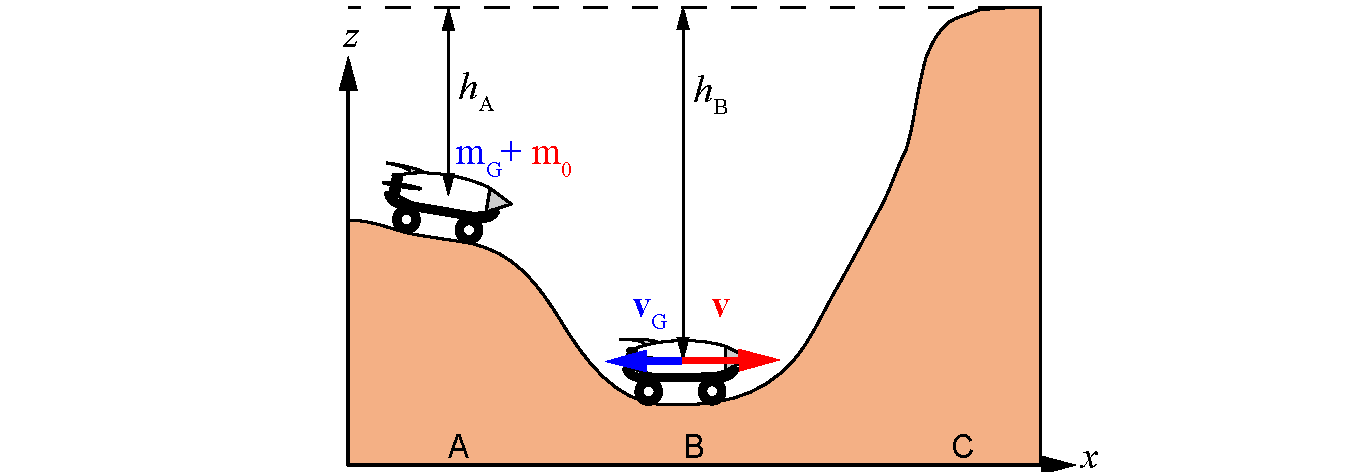
\includegraphics[width=\textwidth]{OberthEffAnalogie.pdf} 
	\caption[Analogie-Modell zum Oberth-Effekt.]{Analogie-Modell zum Oberth-Effekt.}
	\label{abb:adyn_rocket_analogy02}
\end{figure}

Die gesamte Ver�nderung der kinetischen Energie vom Raketenauto und Treibstoff muss gleich der freigesetzten chemischen Energie des Treibstoffs $\Delta E_\text{T}$ sein:
\begin{align}
\begin{split}
    \Delta T &= \Delta T_\text{R} + \Delta T_\text{G} \\
    &=\frac{1}{2}\,m_\text{G}\,v_\text{G}{}^2 + \frac{1}{2}\,m_0\lk\Delta v\rk^2 + \underbrace{m_0\,v\,\Delta v - m_\text{G}\,v\,v_\text{G}}_{\text{wegen \eqref{eq:adyn_rocket_analogy02}} =0} \\
    \Delta T &= \frac{1}{2}\,m_\text{G}\,v_\text{G}{}^2 + \frac{1}{2}\,m_0\lk\Delta v\rk^2 = \Delta E_\text{T}\,. 
\end{split} \label{eq:adyn_rocket_analogy04}
\end{align}
Die gesamte kinetische Energie ist wie erwartet unabh�ngig von $v$ und wegen der Energieerhaltung gleich $\Delta E_\text{T}$. \\

Was bedeutet das nun f�r den Z�ndungszeitpunkt? Wir untersuchen zwei Zeitpunkte (\bzw Orte) $A$ und $B$. 
Es gilt f�r die Gesamtenergien vor dem Z�nden:
\begin{align*}
    E_\text{A} &= -\lk m_0+ m_\text{G}\rk\,g\,h_\text{A}  \,,\\
    E_\text{B} &= -\lk m_0 + m_\text{G} \rk\,g\,h_\text{B} + T_\text{B} \\
    &= -\lk m_0+m_\text{G}\rk\,g\,h_\text{B}  + \frac{1}{2}\lk m_\text{G} +m_0\rk\,v_\text{B}{}^2 = -\lk m_0 + m_\text{G} \rk\,g\,h_\text{A}     \,.
\end{align*}
Aus $E_\text{A} = E_\text{B}$ folgt $v_\text{B} = \sqrt{2g\lk h_\text{B} -h_\text{A}\rk }$.\\

Unmittelbar nach dem Z�nden am Punkt $B$ gilt:
\begin{align*}
    E_\text{R}' =\,&\frac{1}{2}\,m_0\lk v_\text{B}+\Delta v\rk^2 - m_0\,g\,h_\text{B} + \frac{1}{2}\,m_\text{G}\lk v_\text{B} -v_\text{G}\rk^2 - m_\text{G}\,g\,h_\text{B}\\
    = \,&\frac{1}{2}\,m_0\lk\Delta v\rk^2 + m_0\,g\,h_\text{A} -m_0\,\Delta v\,\sqrt{2g\lk h_\text{B}-h_\text{A}\rk} \,,\\
		E_\text{G}' = \,& \frac{1}{2}\,m_\text{G}\,v_\text{G}{}^2 -m_\text{G}\,g\,h_\text{A} - m_\text{G}\,v_\text{G}\,\sqrt{2g\lk h_\text{B}-h_\text{A}\rk} \,,\\
    E_\text{ges}' = \,&\frac{1}{2}\,m_0\,\lk\Delta v\rk^2 + \frac{1}{2}\,m_\text{G}\,v_\text{G}{}^2 - \lk m_0 + m_\text{G}\rk\,g\,h_\text{A} = \, E_\text{A} + \Delta E_\text{T} \,.
\end{align*}
Man erkennt, dass die Energie der Rakete einen von $\sqrt{\lk h_\text{B} -h_\text{A}\rk}$ abh�ngigen Term hat, der offensichtlich verschwindet, wenn $h_\text{B} = h_\text{A}$ ist, es also keine Potentialmulde gibt. \\
Wir bestimmen jetzt noch wie gro� $\Delta v$ sein mu�, um den Punkt C zu erreichen, wenn die Rakete bei $B$ gez�ndet wird. 
\begin{align}
\begin{split}
    \frac{1}{2}\,m_0\,v_\text{C}{}^2 &= \frac{1}{2}\,m_0\,\lk \Delta v\rk^2 - m_0\,g\,h_\text{A} +m_0\,\Delta v \,\sqrt{2g\lk h_\text{B}-h_\text{A}\rk}\\
    \rightarrow ~~~~ 0 &= \lk \Delta v\rk^2 + 2\,\Delta v\,\sqrt{2g\lk h_\text{B}-h_\text{A}\rk} - 2\,g\,h_\text{A}\\
    \rightarrow ~~~~ \lk \Delta v\rk_\text{min} &= \sqrt{2g\lk h_\text{B}-h_\text{A}\rk} + \sqrt{\frac{g}{2}\,\lk h_\text{B}-h_\text{A}\rk + 2\,g\,h_\text{A}} 
\end{split}\,.\label{eq:adyn_rocket_analogy06}
\end{align}
Wie erwartet wird $\Delta v$ f�r $h_\text{B} = h_\text{A}$ zu $\Delta v= \sqrt{2\,g\,h_\text{A}}$. \\
Wir haben $\Delta v\lk h_\text{B}, h_\text{A}\rk$ in \figref{adyn_rocket_analogy03} dargestellt.\\

Die Analogie zum Oberth-Effekt der Raumfahrt ist offensichtlich. Wenn man den gr��tm�glichen beschleunigenden Effekt auf ein Raumschiff haben will, startet man das Man�ver am Punkt der Bahn, wo die Geschwindigkeit am gr��ten ist, \dh im Perig�um oder allgemein an der Periapsis. \\
Einfach gesprochen besagt der Oberth-Effekt, dass ein Raumschiff bei einem Impulsman�ver etwas Energie zus�tzlich zur chemischen Energie des Treibstoffs  \anf{stehlen} kann und zwar von der urspr�nglichen kinetischen Energie, die der Treibstoff vor dem Z�nden auf Grund der Bewegung der Rakete hatte. Anders gesagt: Der Schub generiert einen Impuls proportional zu $\Delta v$. Da die Energie proportional zu $v^2$ ist, ist dieser generierte Impuls energetisch um so wirksamer, je gr��er die Geschwindigkeit $v$ zu Beginn des Schubs ist.


\begin{figure}[H]
	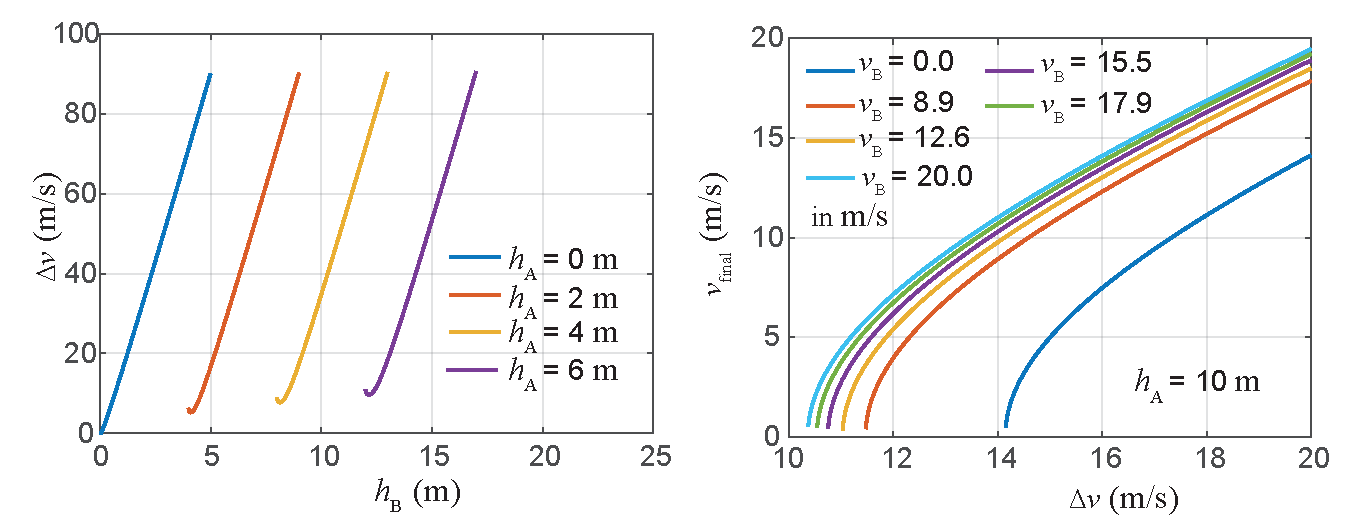
\includegraphics[width=\textwidth]{OberthEffAnalogie02.pdf} 
	\caption[Antriebsbedarf eines Raketenautos durch eine Potentialmulde.]{Antriebsbedarf eines Raketenautos durch eine Potentialmulde als Analogie-Modell zum Oberth-Effekt (Parameter siehe \mscr~\mladynref{OberthEffektAnalogie.m}).}
	\label{abb:adyn_rocket_analogy03}
\end{figure}

\end{sol} 
\textcolor{blue} {$\rightarrow$ zur} \probref{adyn_rocket_analogy}.\\
\noindent\rule[1ex]{\textwidth}{0.5pt}  \newpage  \clearpage


%-----------------------------------------------------------------------------------------------------------

\begin{sol}{prob:adyn_manoevers1}\label{lsg:adyn_manoevers1} %�bung12
\textbf{Hohmann-Transfer}
\begin{itemize}
   \item �bergangszeit f�r den Hohmann-Transfer als Funktion von $r_2/r_1$ \\
	Die �bergangszeit ergibt sich als halbe Umlaufzeit f�r die Hohmann-Ellipse:
	\begin{align*}
    t_\text{H} = \pi\sqrt{\frac{a_\text{H}{}^3}{m_\text{ZK}\,G}} = \frac{\pi}{\sqrt{m_\text{ZK}\,G}}\,\sqrt{\lk \frac{r_1+r_2}{2}\rk^3}\,.
\end{align*}
F�r den Fall eines Hohmann-Transfers von der Erdbahn in den interplanetaren Raum sind die Zeiten in \figref{adyn_Hohmann_TOF} dargestellt (\mscr~\mladynref{HohmannTransfer.m}).
\begin{figure}[H]
	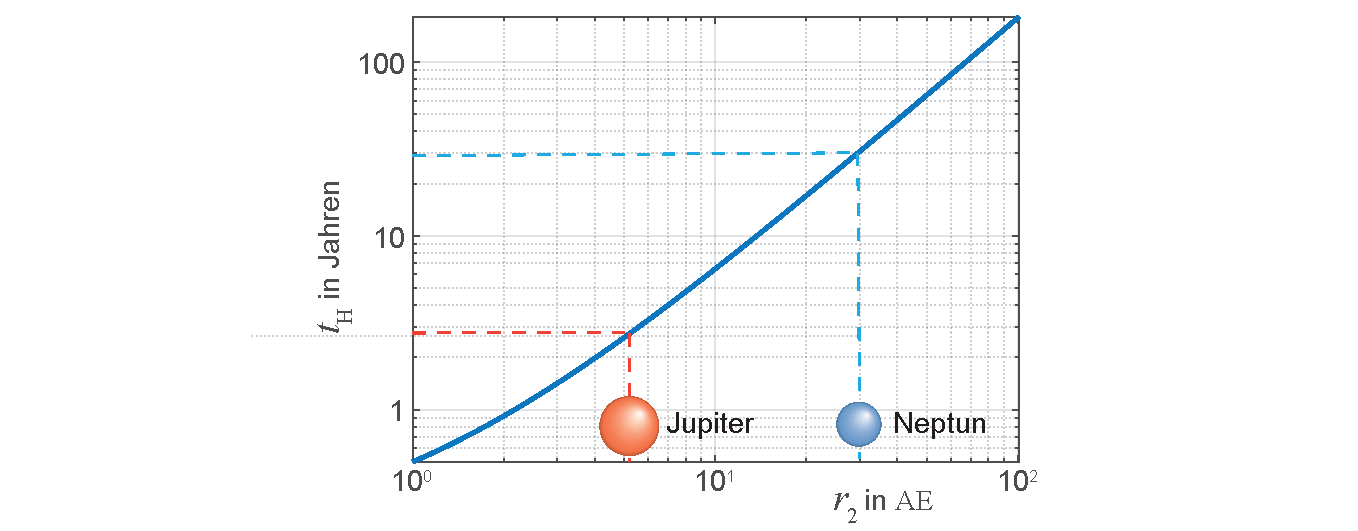
\includegraphics[width=\textwidth]{HohmannTOF.pdf} 
	\caption[Hohmann-Transferzeiten.]{Hohmann-Transferzeiten.}
	\label{abb:adyn_Hohmann_TOF}
\end{figure}
   \item $\Delta v$ gr��er als die \gls{vescape}\\
	F�r $r_2 \rightarrow \infty$ geht $\Delta v_2 \rightarrow 0$ und $\Delta v_1 \rightarrow v_\text{F}$. Daher ist in einem Bereich von $3.3 < r_2/r_1 < \infty$ die Summe $\Delta v_1+\Delta v_2$ gr��er als $v_\text{F}$, wie man leicht aus \eqref{eq:adyn_hohmann04} zusammen mit \eqref{eq:adyn_hohmann03a} und  \eqref{eq:adyn_hohmann03b} herleiten kann.\\
	Im Allgemeinen braucht man insgesamt mehr Antriebsenergie wenn eine Raumsonde erst impulsiv beschleunigt wird, dann durch Gravitation verlangsamt wird und anschlie�end wieder beschleunigt wird, als wenn die gesamte Antriebsimpuls in der Form von $\Delta v_1 = v_\text{F}$ aufgebracht wird.\\
   \item Hohmann-Transfer f�r Verringerung des Bahnradius\\
	Beim Hohmann-�bergang von h�heren auf niedrigere Bahnen gelten die Formeln unver�ndert, der Antriebsbedarf ist negativ und als Schub gegen die Flugrichtung zu verstehen.\\
\end{itemize}

\end{sol} 
\textcolor{blue} {$\rightarrow$ zur} \probref{adyn_manoevers1}.\\
\noindent\rule[1ex]{\textwidth}{0.5pt}  \newpage  \clearpage

%-----------------------------------------------------------------------------------------------------------
\begin{sol}{prob:adyn_manoevers2}\label{lsg:adyn_manoevers2} %�bung13
\textbf{Bielliptischer �bergang}\\

Zwei-Impuls-�bergang von Bahn mit Radius $r_1$ auf eine elliptische Bahn mit Radius $r_2$: 
F�r den Hohmann-Transfer nach $\infty$ ($r_2 \to\infty)$ k�nnen wir schreiben:
\begin{align*}
    \Delta v_1 = \sqrt{\frac{\mu}{r_1}}\,\lk \sqrt{2}-1\rk = v_1\lk \sqrt{2}-1\rk\,.
\end{align*}
Hierin ist $\mu$ der Gravitationsparameter f�r den jeweiligen betrachteten Zentrlk�rper (Erde, Sonne). Analog folgt in der umgekehrten Richtung (aus dem $\infty$ auf die Kreisbahn $r_2$):
\begin{align*}
    \Delta v_2 = v_2 \lk \sqrt{2}-1 \rk
\end{align*}
und somit mit $ \gamma = r_2 / r_1$:
\begin{align*}
    \frac{\Delta v_2}{v_1} = \frac{v_2}{v_1}\,\lk \sqrt{2}-1\rk = \sqrt{\frac{r_1}{r_2}} \,\lk\sqrt{2}-1\rk = \frac{\sqrt{2}-1}{\sqrt{\gamma}}\,.
\end{align*}
Der Gesamt-Antriebsbedarf ist dann: 
\begin{align*}
    \frac{\Delta v}{v_1} = \frac{\Delta v_1+\Delta v_2}{v_1} = \frac{\Delta v_1}{v_1}+\frac{\Delta v_2}{v_1} = \lk \sqrt{2} -1\rk\lk 1 + \frac{1}{\sqrt{\gamma}}\rk\,.
\end{align*}
\begin{figure}[H]
	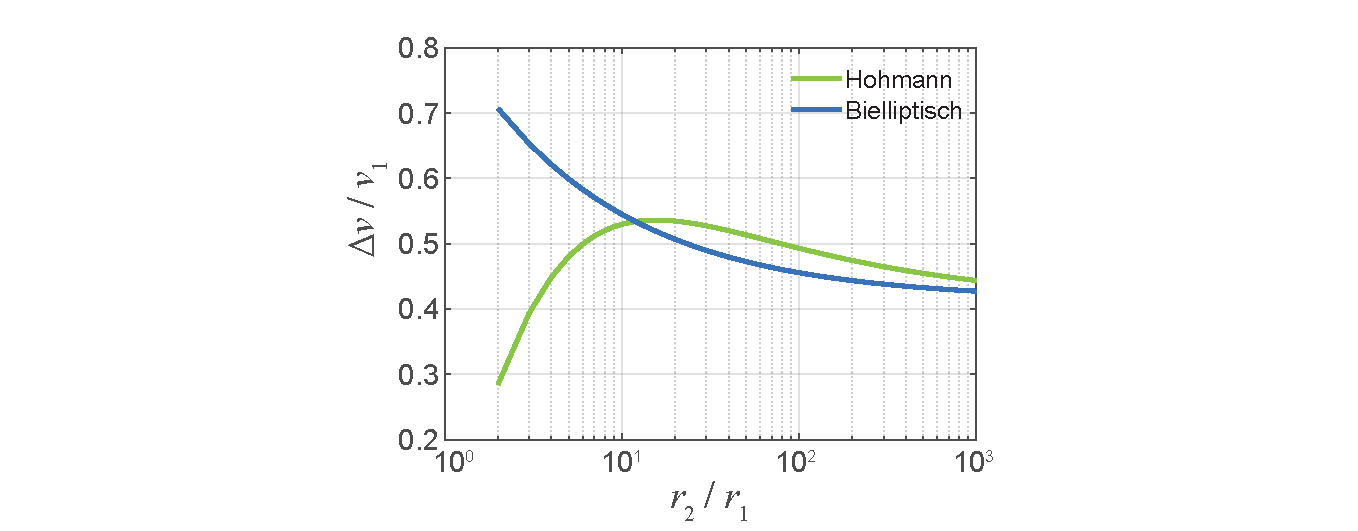
\includegraphics[width=\textwidth]{BiEllptischerTransfer.pdf} 
	\caption[Bielliptischer Transfer.]{Antriebsbedarf beim bielliptischen Transfer im Vergleich zum Hohmann-Transfer.}
	\label{abb:adyn_manoevers2}
\end{figure}

Man erkennt aus \figref{adyn_manoevers2}, dass in der Tat f�r gro�e Radienverh�ltnisse ($\gamma > \SI{11.94}{}$) der bielliptische-Transfer energetisch g�nstiger ist.\\
Allerdings erkauft man sich das durch sehr lange Transferzeiten. Vorteilhaft sind solche bielliptischen �berg�nge aber, wenn man die Inklination und Umlaufrichtung des Orbits �ndern will. Die Rechnungen sind im Detail im \mscr~\mladynref{BiElliptischerTransfer.m} ausgef�hrt.
Die in der Abbildung gezeigten Trajektorien der hyperbolischen Bahnen sind nach \kap{hm_bewegungsgl} gegeben durch:
\begin{align}
	 r = \frac{a\,\lk 1 - e^2 \rk}{1 - e\,\cos\upsilon} ~~~\text{mit}~~~\upsilon < \arccos\frac{1}{e} ~~~\text{und}~~~a = \frac{r_\text{P}}{(1-e)} \,.	\label{eq:adyn_oberth37}
\end{align}
Die geometrischen Parameter $a$ und $e$ der Hyperbel sind durch die physikalischen Parameter $H$ \bzw $v_\infty$ und $r_\text{P}$ definiert (vgl. \kap{hm_bewegungsgl}: $~a < 0,\, e > 1$):
\begin{align}
	 a = -\frac{\mu}{2H_\infty} = -\frac{\mu}{v_\infty{}^2} ~~~\text{und}~~~e = 1 + \frac{r_\text{P}\,v_\infty{}^2}{\mu} \,.	\label{eq:adyn_oberth38}
\end{align}

\end{sol} 
\textcolor{blue} {$\rightarrow$ zur} \probref{adyn_manoevers2}.\\
\noindent\rule[1ex]{\textwidth}{0.5pt}  \newpage  \clearpage

%-----------------------------------------------------------------------------------------------------------

\begin{sol}{prob:adyn_manoevers3}\label{lsg:adyn_manoevers3} %�bung14
\textbf{Hohmann-Oberth-Edelbaum-Transfers aus dem Orbit nach $\infty$}\\

Die Rechnungen sind explizit im \mscr~\mladynref{TransferUnendlich.m} hinterlegt und die Ergebnisse in \figref{adyn_Oberth_transfer2} und \figref{adyn_Oberth_transfer3} gezeigt. 
Man erkennt, dass es f�r gr��ere finale Abst�nde $r_\text{end}$ und bestimmte Verh�ltnisse von $r_{+}/r_1$  ein Minimum der Flugzeit f�r den Edelbaum-Transfer gibt. Er ist in den meisten F�llen der energetisch g�nstigste Transfer. Der Hohmann-Transfer ist f�r gro�e Entfernungen sowohl was die Flugzeit als auch den Antriebsbedarf betrifft der ung�nstigste.\\

\begin{figure}
	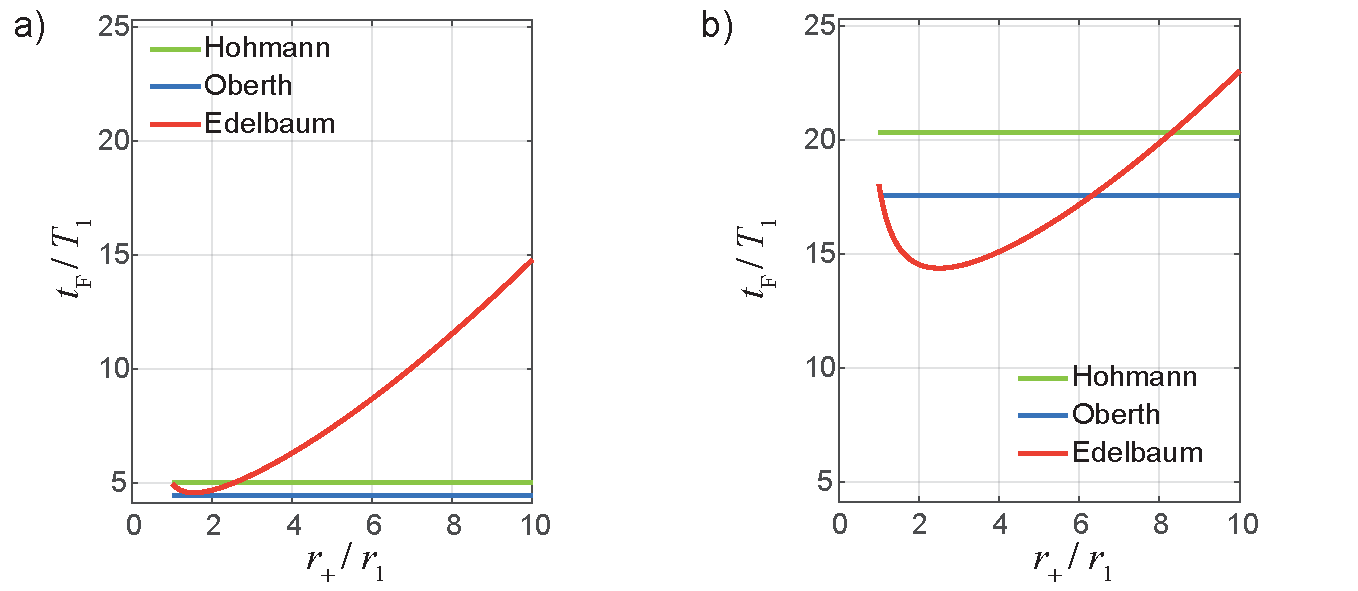
\includegraphics[width=\textwidth]{TransfersInfin03.pdf} 
	\caption[Flugzeiten beim Transfer nach $\infty$.]{Flugzeiten beim Hohmann-, Oberth- \bzw Edelbaum-Transfer. \fa bis zu $r_\text{end}=50\,r_1$ \fb bis zu $r_\text{end}=200\,r_1$.  Als variabler Parameter wurde der �u�ere Radius $r_{+}$ genommen, der innere Radius wurde als fix mit $r_{-}=0.05\,r_1$ gesetzt und der Schubparameter wurde mit $\Delta v/v1 = 1.1$ angenommen. Man erkennt, dass es f�r $r_{+}\approx 2.5\,r_1$ ein absolutes Minimum der Flugzeit f�r den Edelbaum-Transfer gibt. Danach f�hrt die l�ngere Flugzeit auf der Halbellipse von $r_{+}$ nach $r_{-}$ zu insgesamt l�ngeren Flugzeiten.} \label{abb:adyn_Oberth_transfer3}
\end{figure}

\end{sol} 
\textcolor{blue} {$\rightarrow$ zur} \probref{adyn_manoevers3}.\\
\noindent\rule[1ex]{\textwidth}{0.5pt}  \newpage  \clearpage

%-----------------------------------------------------------------------------------------------------------

\begin{sol}{prob:adyn_manoevers4}\label{lsg:adyn_manoevers4} %�bung15
\textbf{Lambert-Problem}\\

Die allgemeine Formulierung des Lambert-Problems lautet wie folgt (\figref{adyn_lambert_lsg02a}):\\
Es seien zwei Punkte $\text{P}_1,\, \text{P}_1$ im Raum durch ihre Vektoren $\vec{r}_1$, $\vec{r}_2$ bekannt, ebenso die Zeit $t_\text{F} = t_2-t_1$, die f�r die Bewegung des K�rpers zwischen $\mathrm{P}_1$ und $\mathrm{P}_2$ ben�tigt wird. Gesucht sind f�r die Kepler-Ellipse die Bahnparameter $a$, $e$, $ \upsilon_0$.\footnote{Wir wollen hier nur Ellipsenbahnen betrachten. Man kann das Problem auch f�r Hyperbelbahnen formulieren und l�sen, siehe \ua \cite{Izzo2015, Walter2018}. Im wesentlichen werden dabei die Winkelfunktionen durch die Hyperbelfunktionen ersetzt.}\\

\begin{figure}[H]
	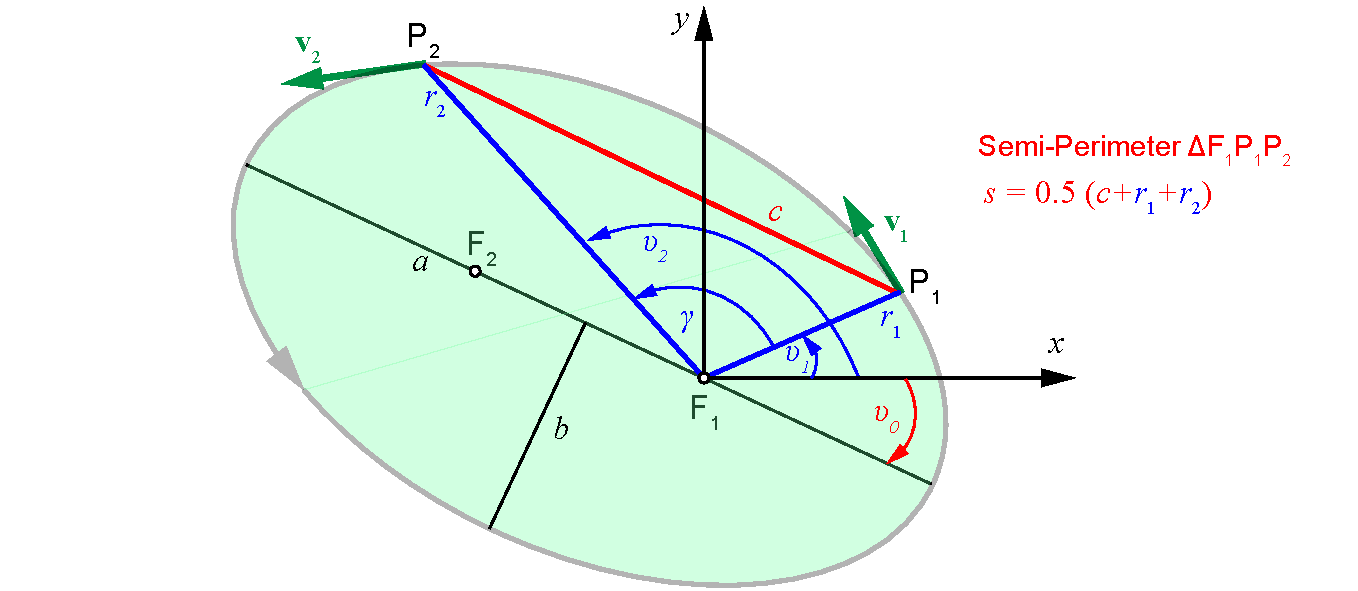
\includegraphics[width=\textwidth]{LambertProblem02Geometrie.pdf} 
	\caption[Geometrie des Lambert-Problems.]{Geometrie des Lambert-Problems. Parameter siehe Text.}
	\label{abb:adyn_lambert_lsg02a}
\end{figure}

Zun�chst schreiben wir die Kepler-Gleichung f�r die beiden Zeitpunkte auf ($\mu$ ist hierin der Gravitationsparameter des Zentralk�rpers, in dessen Schwerefeld die Bewegung stattfindet.) und subtrahieren die beiden Gleichungen voneinander. Wir erhalten:
\begin{align}
\sqrt{\frac{\mu}{a^3}}\,\lk t_2-t_1\rk &= \sqrt{\frac{\mu}{a^3}}\,t_\text{F} = E\lk t_2\rk - E\lk t_1\rk -e\,\lek \sin E\lk t_2\rk -\sin E\lk t_1\rk\rek \nonumber \\
\rightarrow ~~~~ \sqrt{\frac{\mu}{a^3}} \,t_\text{F} &= E_2-E_1 -e\,\lk \sin E_2 -\sin E_1\rk \label{eq:adyn_lsglambert01}\,.
\end{align}
Durch die Randwerte ist ja ein Brennpunkt der Ellipse, n�mlich $\mathrm{F}_1$ bekannt. Man sucht nun den Brennpunkt $\mathrm{F}_2$ (oft auch versteckter Fokus genannt), mit dem dann die Ellipse eindeutig definiert ist und zugleich die Bedingung erf�llt ist, dass f�r das Durchlaufen von $\mathrm{P}_1$ nach $\mathrm{P}_2$ die Zeit $t_\text{F}$, im Englischen auch \gls{ToF} (ToF), ben�tigt wird. 

\begin{figure}[H]
	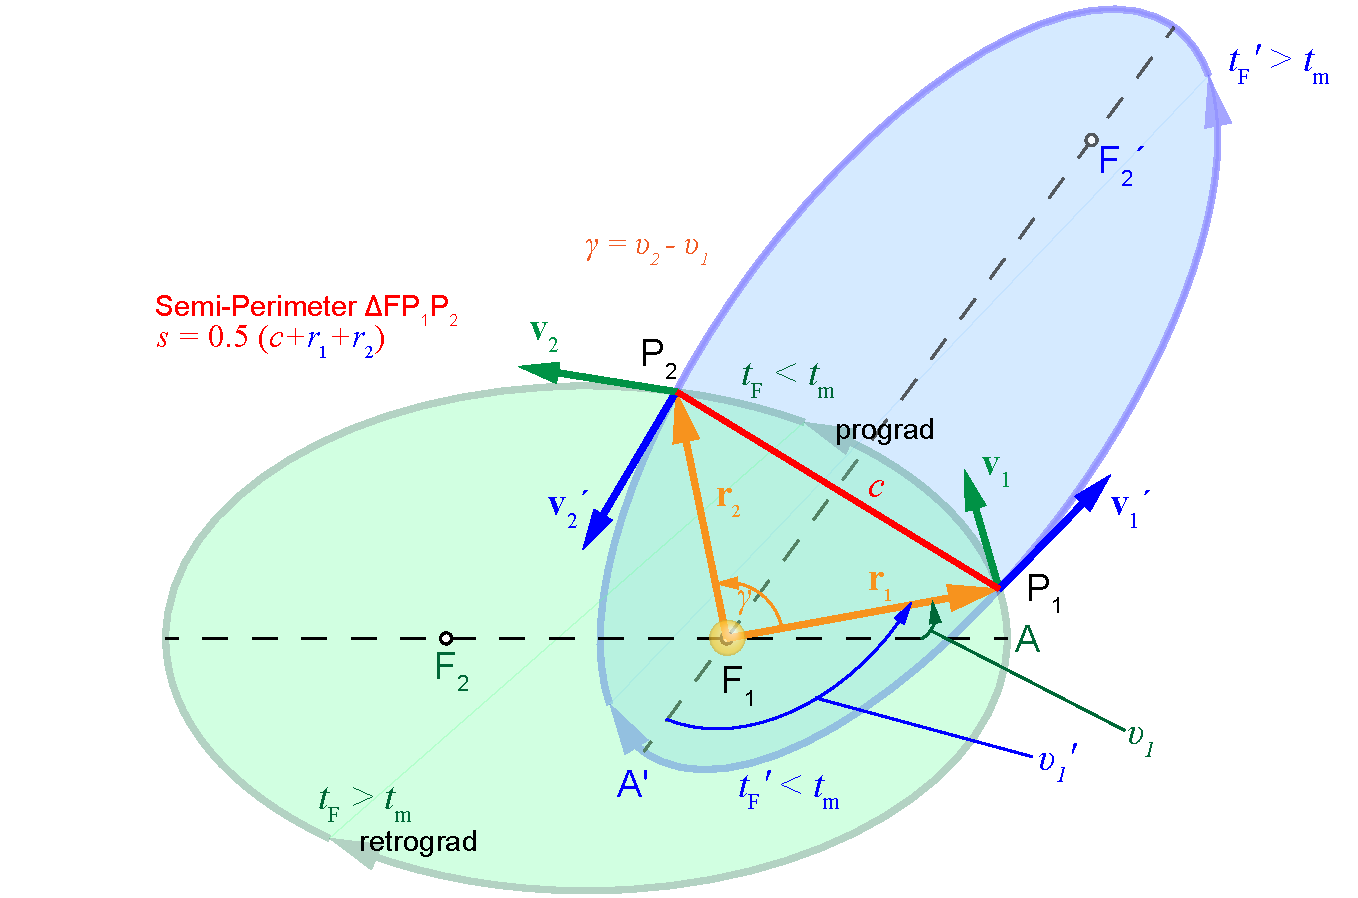
\includegraphics[width=\textwidth]{LambertProblem02Allgemein.pdf} 
	\caption[Geometrie des Lambert-Problems.]{Geometrie des Lambert-Problems. Die beiden Ellipsen (gr�n und blau schattiert) stellen jeweils eine L�sung des Lambert-Problems f�r unterschiedliche Flugzeiten und Flugrichtungen dar. Die Flugrichtung wird als prograd bezeichnet, wenn diese entgegen des Uhrzeigersinns von $\mathrm{P}_1$ nach $\mathrm{P}_2$ erfolgt, die entgegengesetzte Flugrichtung wird retrograd genannt. Die Vektoren $\vec{r}_1$, $\vec{r}_2$ definieren die Ellipsen, sie k�nnen als Positionsvektoren aber auch zu unterschiedlichen Umlaufbahnen geh�ren, \zb $\vec{r}_1$ kann ein Vektor von der Sonne zur Erde sein, $\vec{r}_2$ eine entsprechender Vektor zum Mars. Weitere Parameter siehe Text.}
	\label{abb:adyn_lambert_lsg02}
\end{figure}
Wir k�nnen uns nun leicht �berlegen, dass es f�r die gesuchte Bahn zwei Ellipsen als denkbare L�sungen gibt und zwar mit den beiden "`versteckten"' Fokuspunkten $\mathrm{F}_2$ und $\mathrm{F}_2{}'$ (\figref{adyn_lambert_lsg02})\footnote{Man kann sich die zwei L�sungen anschaulich-geometrisch deutlich machen, in dem man sich die Konstruktionsvorschrift einer Ellipse in Erinnerung ruft. Nach dieser ist an jedem Punkt einer Ellipse die Summe des Abstandes zu den beiden Fokuspunkten konstant und gleich $2a$. Die Konstruktion erfolgt, in dem man einen Kreis um $\mathrm{P}_1$ mit dem Radius $2a-r_1$ schl�gt und einen um $\mathrm{P}_2$ mit $2a-r_2$. Es ergeben sich zwei Schnittpunkte, dies sind die Brennpunkte $\mathrm{F}_2$ \bzw $\mathrm{F}_2{}'$.}.\\
Mit den Beziehung \eqref{eq:hm_r_param_ellipse} und \eqref{eq:hm_bahnglg} aus dem \kap{hm_abl_kepler} k�nnen wir schreiben: 
\begin{subequations}
\begin{align}
    r_{1,2} &= a\,\lk 1-e\,\cos E_{1,2}\rk  \label{eq:adyn_lsglambert02a} \,,\\
    \cos\lk \upsilon_{1,2}-\upsilon_0\rk &= \frac{a}{r_{1,2}}\,\lk\cos E_{1,2}-e\rk \,. \label{eq:adyn_lsglambert02b}
    %r_{1,2}\cos{\upsilon_{1,2}} &= a\,\lk \cos E_{1,2} - e \rk \,, \label{eq:adyn_lsglambert02b} \\
    %r_{1,2}\sin{\upsilon_{1,2}} &= a\,\sqrt{\lk 1-e^2 \rk}\, \sin E_{1,2} \,, \label{eq:adyn_lsglambert02c} \\
\end{align} %\label{eq:adyn_lsglambert02} 
\end{subequations}
Wir betrachten eine der beiden Ellipsen aus \figref{adyn_lambert_lsg02} genauer und verwenden die Darstellung in \figref{adyn_lambert_lsg02a}. Unser Ziel ist es ja, die Trajektorie $r(\upsilon)$ zu finden:
\begin{align}
    r (\upsilon) &= \frac{a\,\lk 1 - e^2 \rk}{1+e\,\cos\lk\upsilon - \upsilon_0 \rk}\,. \label{eq:adyn_lsglambert_traj} 
\end{align} 
In einer Ebene ist eine Trajektorie (Bahn) durch 3 Parameter eindeutig bestimmt. Das Lambert-Problem ist ein planares Problem und wir
haben mit dem Gleichungssystem \eqref{eq:adyn_lsglambert01}, \eqref{eq:adyn_lsglambert02a} und \eqref{eq:adyn_lsglambert02b} ein System f�r 5 Unbekannte $E_1$, $E_2$, $a$, $e$, $\upsilon_0$ mit den bekannten Gr��en $r_1$, $r_2$, $\upsilon_1$, $\upsilon_2$, $t_\text{F}$ und $\mu$.\footnote{Eigentlich sind $\upsilon_1$, $\upsilon_2$ ja nicht bekannt, sondern nur deren Differenz. Durch freie Festlegung eines \KOS wie in \figref{adyn_lambert_lsg02a} gezeigt kann man sich aber $\upsilon_1$ und $\upsilon_2$ berechnen. Man beachte, dass dieses \KOS mit den $x-y$- Achsen in der Ellipsenebene liegt und gegebenenfalls durch Drehung in ein anderes (\zb heliozentrisches) \KOS transformiert werden muss, wenn man die koordinaten der Trajektorie in diesem haben  m�chte.} Dieses System wollen wir jetzt l�sen:
\begin{enumerate}
    \item [1.] Mit der Nebenrechnung (\cite{Gradshteyn1980})
		\begin{align*}
		\sin x - \sin y =&  \sin{\lk \frac{x-y}{2} +  \frac{x+y}{2}\rk} - \sin{\lk \frac{x+y}{2} +  \frac{-x+y}{2}\rk} \\
		=& \sin{\lk \frac{x-y}{2} +  \frac{x+y}{2}\rk} + \sin{\lk \frac{x-y}{2} + \frac{-x-y}{2} \rk} \\
		=& \sin\lk \frac{x-y}{2}\rk\,\cos\lk\frac{x+y}{2}\rk + \sin\lk \frac{x+y}{2}\rk\,\cos\lk\frac{x-y}{2}\rk\\
		&+ \sin\lk \frac{x-y}{2}\rk\,\cos\lk\frac{x+y}{2}\rk - \sin\lk \frac{x+y}{2}\rk\,\cos\lk\frac{x-y}{2}\rk \\
		=& 2\,\sin{\frac{x-y}{2}}\,\cos{\frac{x+y}{2}}
		\end{align*}
    f�hren wir $\psi$ und $\varphi$ als neue Variable ein:
    \begin{align}
        \psi = \frac{E_2-E_1}{2}~~~~ \text{und} ~~~~ \cos \varphi = e\,\cos\lk \frac{E_2 +E_1}{2} \rk \,, \label{eq:adyn_lsglambert06}
    \end{align}
		wobei $\psi \in [0, \pi]$ und $\varphi \in [0, \pi]$ gilt. Wir erhalten dann die Kepler-Gleichung \eqref{eq:adyn_lsglambert01} in folgender vereinfachter Form:
\begin{align}
			\sqrt{\frac{\mu}{a^3}} \,t_\text{F} &= \psi - \cos\varphi\, \sin\psi \label{eq:adyn_lsglambert01a}\,.
\end{align}
Die beiden Gr��en $\psi$ und $\varphi$ h�ngen nur von der vorgegebenen Geometrie des Problems ab, wie man leicht nachrechnen kann, in dem man 
den Abstand von $\mathrm{P}_1$ und $\mathrm{P}_2$ unter Verwendung von \eqref{eq:adyn_lsglambert02b} �ber 
    \begin{align}
        c^2 &= \lk r_2\,\cos\upsilon_2 - r_1\,\cos\upsilon_1 \rk^2 + \lk r_2\,\sin\upsilon_2 - r_1\,\sin\upsilon_1 \rk^2 ~\nonumber \\
				&= r_1{}^2+r_2{}^2 - 2\,r_1\,r_2\,\cos\lk \upsilon_2-\upsilon_1\rk = r_1{}^2+r_2{}^2 - 2\,r_1\,r_2\,\cos\lk \gamma \rk~\nonumber \\
				\rightarrow~~c &= 2 a\,\sin\psi\,\sin\varphi\, \label{eq:adyn_lsglambert03a}
    \end{align}
berechnet. 
Ebenso erh�lt man die Summe der Abst�nde $r_1+r_2$ von den Punkten $\mathrm{P}_1$ und $\mathrm{P}_2$ zum Brennpunkt $\mathrm{F}_1$ wiederum unter Verwendung von \eqref{eq:adyn_lsglambert02b} zu
		\begin{align}
		r_1 + r_2  &= 2a\lk 1- \cos\psi\, \cos\varphi \rk\,. \label{eq:adyn_lsglambert03b}
    \end{align} 
Die Gleichungen \eqref{eq:adyn_lsglambert03a} und \eqref{eq:adyn_lsglambert03b} bestimmen die Gr��en $\psi$ und $\varphi$ eindeutig. Man kann also schlussfolgern, dass die Zeit $t_\text{F}$ nach \eqref{eq:adyn_lsglambert01a} nur eine Funktion von $a$ und den bekannten geometrischen Gr��en $c$ und $r_1 + r_2$  ist.\footnote{Der Beweis daf�r wurde von Lagrange erbracht, der zeigte, dass die ToF $t_\text{F}$ nur von der Energie der Bahn und damit nur von $a$ abh�ngt.}\\   

\item [2.] Um uns die Rechnungen zu erleichtern, f�hren wir zwei weitere Gr��en ein, die wir aus $\varphi$ und $\psi$ wie folgt bilden:
				\begin{align}
						\alpha= \varphi +\psi ~~~~ \text{und} ~~~~ \beta= \varphi-\psi \,. \label{eq:adyn_lsglambert05}
				\end{align}
		Offensichtlich gilt: $\alpha \in [0,\, 2\pi]$ und $\beta \in [-\pi,\, \pi]$. \\
		
\item [3.] Wir bezeichnen den halben Umfang (Semi-Perimeter) des Dreiecks $\Delta \,\mathrm{F}_1\mathrm{P}_1\mathrm{P}_2$ mit 
    \begin{align}
        s= \frac{r_1+r_2+c}{2}\,. \label{eq:adyn_lsglambert04}
    \end{align}
		Damit und mit \eqref{eq:adyn_lsglambert03a} und \eqref{eq:adyn_lsglambert03b} findet man  f�r $\alpha$ die Beziehung: 
    \begin{subequations}
    \begin{align}
        \frac{s}{2a} &= \frac{1}{2} \lek 1 - \cos\psi\cos\varphi + \sin\psi\sin\varphi \rek = \frac{1}{2} \lek 1 - \cos \lk \psi+\varphi \rk \rek \nonumber \\
				&= \frac{1}{2} \lek 1 - \cos\alpha \rek = \frac{1}{2} \lek 1 - \cos\lk \frac{\alpha}{2} + \frac{\alpha}{2} \rk \rek \nonumber \\
				&= \frac{1}{2} \lek 1 - \cos^2\frac{\alpha}{2} + \sin^2\frac{\alpha}{2} \rek = \frac{1}{2} \lek 2\sin^2\frac{\alpha}{2} \rek \nonumber \\
        &\rightarrow~~ \sin^2\lk \frac{\alpha}{2}\rk = \frac{s}{2a}\, \label{eq:adyn_lsglambert06a} \\
				&\text{und entsprechend f�r}~~ \beta \nonumber \\
        &\rightarrow~~ \sin^2\lk\frac{\beta}{2}\rk = \frac{s-c}{2a}\,\label{eq:adyn_lsglambert06b}
    \end{align}
    \end{subequations}
    Sowohl $\alpha$ als auch $\beta$ sind somit Gr��en, die nur von der Geometrie der Aufgabenstellung und dem Bahnparameter $a$ abh�ngen.\\
		
\item [4.] Wir setzen nun \eqref{eq:adyn_lsglambert06a} und \eqref{eq:adyn_lsglambert06b} in \eqref{eq:adyn_lsglambert01} ein und erhalten die elegante Formulierung des Lambert-Problems 
\begin{align}
    t_\text{F} &= \sqrt{\frac{a^3}{\mu}}\,\lk \alpha-\beta-\lek\sin\alpha -\sin\beta\rek\rk\,,\label{eq:adyn_lsglambert07}
\end{align}   
Damit haben wir $E_2$, $E_1$ aus der Kepler-Gleichung eliminiert und das Lambert-Problem auf ein System von 3 Unbekannten ($a$, $\alpha$, $\beta$) zur�ck gef�hrt, von den $\alpha$ und $\beta$ neben den bekannten Gr��en $s$, $c$ nur noch von $a$ abh�ngen. Der Winkel $\alpha$ ist dabei wegen des Quadrats in \eqref{eq:adyn_lsglambert06a} nicht eindeutig bestimmt, es gibt zwei L�sungen
\begin{align}
	\alpha ~~~\text{und}~~~ \alpha'=2\pi-\alpha\,, \label{eq:adyn_lsglambert08}
\end{align}
die den beiden Ellipsenl�sungen und damit auch den beiden Zeit $t_\text{F}$ \bzw $t_\text{F}'$ in \figref{adyn_lambert_lsg02} entsprechen. Der Wert f�r $\beta$ ist hingegen f�r ein aus \eqref{eq:adyn_lsglambert08} folgendes  $a$ \bzw $a'$ eindeutig bestimmt. Man muss aber folgende Fallunterscheidung machen: 
\begin{align}
    \beta = \left\{
\begin{array}{ll}
+2\arcsin\sqrt{(s-c)/a} ~~ & \text{f�r} ~~~~ \gamma = \upsilon_2-\upsilon_1 <\pi \\
-2\arcsin\sqrt{(s-c)/a} ~~ & \text{f�r} ~~~~ \gamma = \upsilon_2-\upsilon_1 >\pi \\
\end{array}
\right.\,.\label{eq:adyn_lsglambert09}
\end{align}

\item [5.] Setzen wir $\alpha\lk a,a' \rk$ und $\beta\lk a,a' \rk$ in \eqref{eq:adyn_lsglambert07} ein, erhalten wir demzufolge zwei Kurven $t_\text{F}\lk a\rk$, die vom Punkt $\lek a_\text{min},\, t_\text{m} \rek$ ausgehen (siehe \figref{adyn_lambert_lsg03}). Hierbei ist $a_\text{min} = s/2$, wie man leicht nachpr�fen kann. Die Ellipse, die durch $a_\text{min}$ definiert wird auch Minimal-Energie-Bahn genannt, wegen $E_\text{min}= -\mu/(2a_\text{min})$. Das ist aber nicht zu verwechseln mit dem minimalen Antriebsbedarf $\Delta v_\text{min}$. Ebenso ist $t_\text{m}$ nicht die minimale Flugzeit, sondern die Flugzeit f�r die Bahn mit der kleinsten Bahnenergie. Wie bereits erw�hnt und aus \figref{adyn_lambert_lsg02} zu erkennen, gibt es zu einem bestimmten Wert von $a$ zwei ToF, die dem kurzen ($t_\text{F} < t_\text{m}$) \bzw  der dem langen Transfer ($t_\text{F} > t_\text{m}$) von $\mathrm{P}_1$ nach $\mathrm{P}_2$ entsprechen.\end{enumerate}

Wir wollen nun Gleichung \eqref{eq:adyn_lsglambert07} l�sen. Das ist analytisch nicht m�glich. Da sie aber eine gewisse �hnlichkeit mit der Kepler-Gleichung hat, k�nnen wir �hnliche Iterationsmethoden wie in \kap{iteration_kepler} benutzen. Wir wollen hier das sogenannte Bisektionsverfahren \cite{Arens2008} verwenden. Man geht folgenderma�en vor:
\begin{enumerate}
    %1.
    \item [1.] Wir bestimmenen die Flugzeit f�r eine Parabell�sung von $\text{P}_1$ nach $\text{P}_2$. Diese l�sst sich aus der Barker-Gleichung\index{Barker-Gleichung} \eqref{eq:hm_Barker_glg} bestimmen:\footnote{F�r die interessierten Leser empfehlen wir die Herleitung von \eqref{eq:adyn_lsglambert11} aus der Barker-Gleichung\index{Barker-Gleichung} \eqref{eq:hm_Barker_glg} (siehe  \kap{kometen}) nachzuvollziehen.} % und verweisen auf die Referenzen \cite{Izzo2015}, \cite{Sangra2021}
			\begin{align}
								t_\text{Par} &= \frac{\sqrt{2}}{3}\,\sqrt{\frac{s^3}{\mu}}\,\lk 1-\sqrt{\lk\frac{s-c}{s}\rk^3}\rk\,.\label{eq:adyn_lsglambert11}
			\end{align}
    %2.
    \item [2.] Wir definieren mit \eqref{eq:adyn_lsglambert07} die Funktion\\
			\begin{align}
						\tau\lk a\rk &= \sqrt{\frac{a^3}{\mu}}\,\lek \alpha\lk a\rk -\beta\lk a \rk - \lk \sin\alpha\lk a\rk-\sin\beta\lk a\rk \rk\rek\,.\label{eq:adyn_lsglambert11a}
			\end{align}
    Gesucht ist das $a$, welches $\tau\lk a\rk = t_\text{F}$ erf�llt.
    %3.
    \item [3.] Wir setzen nun $a_\text{min} = s/2$ und bestimmen damit $t_\text{m} = \tau\lk a_\text{min} \rk$. Ist $t_\text{m} > t_\text{F} > t_\text{Par}$,
		so muss eine (elliptische) L�sung existieren.\footnote{F�r $t_\text{F} < t_\text{Par}$ kann man einen hyperbolischen Transfer von $\mathrm{P}_1$ nach $\mathrm{P}_2$ finden, der noch schneller als der parabolische ist. Wir verweisen auf \cite{Izzo2015, Walter2018}.} Ist $t_\text{Par} < t_\text{F} < t_\text{m}$, dann gibt es eine L�sung auf dem unteren Ast in \figref{adyn_lambert_lsg03}, f�r $t_\text{F} > t_\text{m}$ kann es eine L�sung auf dem oberen Ast geben. Man muss das Bisektionsverfahren entsprechend anpassen, siehe dazu auch \mscr~\mladynref{LambertProblem02.m}. 
    %4.
    \item [4.] Wir suchen nun ein $a_\text{max} \gg a_\text{min}$ und setzen $a_1 = (a_\text{min} + a_\text{max})/2$.
    %5.
    \item [5.] Wir bestimmen $\tau\lk a_1\rk$.
    %6.
    \item [6.] Falls $\tau\lk a_1\rk> t_\text{F}$, dann setzen wir $a_2= (a_1+a_\text{max})/2$, falls $\tau\lk a_1\rk <t_\text{F}$, dann setzen wir $a_2 = (a_\text{min}+a_1)/2$.
    %7.
    \item [7.] Wir wiederholen die Schritte bis zur gew�nschten Genauigkeit von $\tau\lk a_n\rk \approx t_\text{F}$. 
\end{enumerate}
Dieses Verfahren konvergiert, falls �berhaupt eine L�sung existiert: deshalb muss man im Schritt 1 �berpr�fen, ob f�r die gegebenen Werte $r_1$, $r_2$, $\gamma$ und $t_\text{F}$ �berhaupt eine elliptische L�sung existiert. 

\begin{figure}[H]
	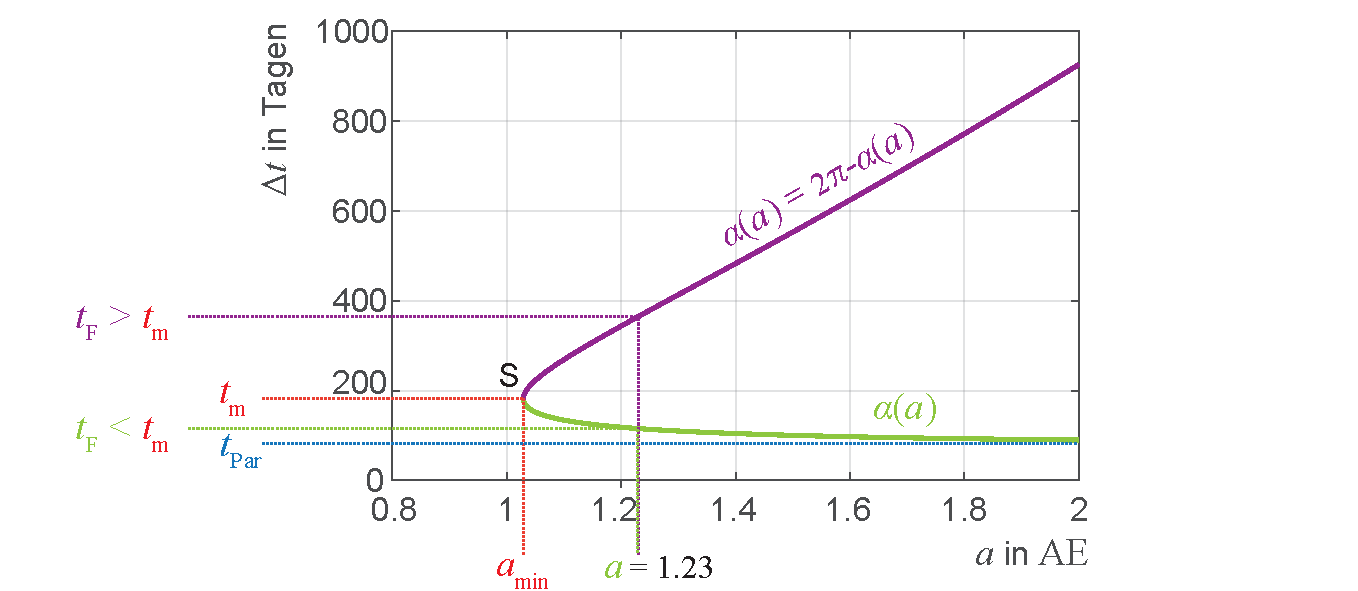
\includegraphics[width=\textwidth]{LambertProblem02Zeiten.pdf} 
	\caption[L�sung des Lambert-Problems.]{L�sung des Lambert-Problems f�r folgende Parameter: $r_1 = \SI{1.0}{AE},\, r_2 = \SI{1.525}{AE},\, \gamma = 75\degree$, und einer ToF von $t_\text{F} = 115 \mathrm{d}$ \bzw $t_\text{F} = 365 \mathrm{d}.$ Siehe \mscr~\mladynref{LambertProblem02.m}.}
	\label{abb:adyn_lambert_lsg03}
\end{figure}
Wir brauchen jetzt noch, nachdem wir $a$ bestimmt haben, die Bahnparameter $e$ und $\upsilon_0$. Aus \eqref{eq:adyn_lsglambert02a} finden wir 
\begin{align}
    E_1 = \arccos \lk \frac{a-r_1}{a\,e} \rk  \label{eq:adyn_lsglambert13}
\end{align}
und aus \eqref{eq:adyn_lsglambert02b} auch $\upsilon_0$
\begin{align}
    \upsilon_0 = \upsilon_1 - 2\,\arctan\lk \sqrt{\frac{1+e}{1-e}}\,\tan\frac{E_1}{2}\rk\,.  \label{eq:adyn_lsglambert14}
\end{align}
Setzen wir das gefundene $a$ in die Gleichungen f�r $\alpha$ und $\beta$ ein und diese wiederum in die f�r $\varphi$ und $\psi$ finden wir mit \eqref{eq:adyn_lsglambert02b} f�r die Exzentrizit�t
\begin{align}
    e = \sqrt{\frac{\lk r_2-r_1\rk^2}{\lk2a\,\sin\psi\rk^2}+\cos^2\varphi}\,.  \label{eq:adyn_lsglambert15}
\end{align}

Hat man mittels Bisektionsverfahren entweder $p$  (mit \mscr~\mladynref{LambertProblem01.m}) oder $a$  (mit \mscr~\mladynref{LambertProblem02.m}) bestimmt, kann man �ber folgende  Beziehung die Geschwindigkeiten an den Punkten $\mathrm{P}_1$ nach $\mathrm{P}_2$ auf der Trajektorie bestimmen (\cite{Walter2018, Battin1999}:
\begin{align}
\begin{split}
    \vec{v}_\text{tr, 1} &= \sqrt{\frac{\mu\,p}{r_1\,r_2\,\sin\gamma}}\,\lek \lk \vec{r}_2 - \vec{r}_1 \rk  + \frac{r_2}{p}\,\lk 1- \cos\gamma \rk\,\vec{r}_1 \rek \\
    \vec{v}_\text{tr, 2} &= \sqrt{\frac{\mu\,p}{r_1\,r_2\,\sin\gamma}}\,\lek \lk \vec{r}_2 - \vec{r}_1 \rk  + \frac{r_1}{p}\,\lk 1- \cos\gamma \rk\,\vec{r}_2 \rek \,.
\end{split}  \label{eq:adyn_lambert16}
\end{align}
Die Richtung der Periapsis (Perihel, Perig�um \usw) und damit der Wert f�r $\upsilon_0$ kann dann �ber den Laplace-Vektor\index{Laplace-Vektor} $\vec{e}$ und \eqref{eq:hm_laplace_int} aus \kap{hm_abl_kepler} wie folgt bestimmt werden:
\begin{align}
    \vec{e} &= \lk \frac{1}{r_1} - \frac{1}{a} \rk \, \vec{r}_1  - \frac{1}{\mu} \, \lk \vec{r}_1 \cdot \vec{v}_\text{tr, 1} \rk \, \vec{v}_\text{tr, 1} \,. 
		\label{eq:adyn_lambert17}
\end{align}

Wir haben das Bisektionsverfahren zur L�sung des Lambert-Problems exemplarisch f�r zwei verschiedene F�lle im \mscr~\mladynref{LambertProblem01.m} \bzw \mscr~\mladynref{LambertProblem02.m} hinterlegt. Fall 1 ist der Transfer einer Raumsonde von der ISS aus $h \approx \SI{422}{\km}$ in die Stratosph�re ($h \approx \SI{22}{\km}$) innerhalb von 50 min und Fall 2 ein Raumflug von der Erde zum Mars f�r eine Flugdauer von 115 Tagen. \figref{adyn_lambert_lsg04} und Tabelle \ref{tab:adyn_bisection} zeigen den Verlauf der Iteration f�r den Fall 2.\\

Im \mscr~\mladynref{LambertProblem03.m} haben wir die Rechnungen mit einer modernen, stabileren numerischen Routine zur L�sung des Lambert-Problems (\cite{Mahooti2015}) wiederholt. Die Routine basiert auf den Ans�tzen, die in \cite{Battin1999, Izzo2015, Walter2018} ausf�hrlich beschrieben sind. Sie beinhaltet auch hyperbolische L�sungen. Die �bereinstimmung mit dem Bisektionsverfahren f�r die angegebenen Beispiele ist sehr gut.

\begin{figure}[H]
	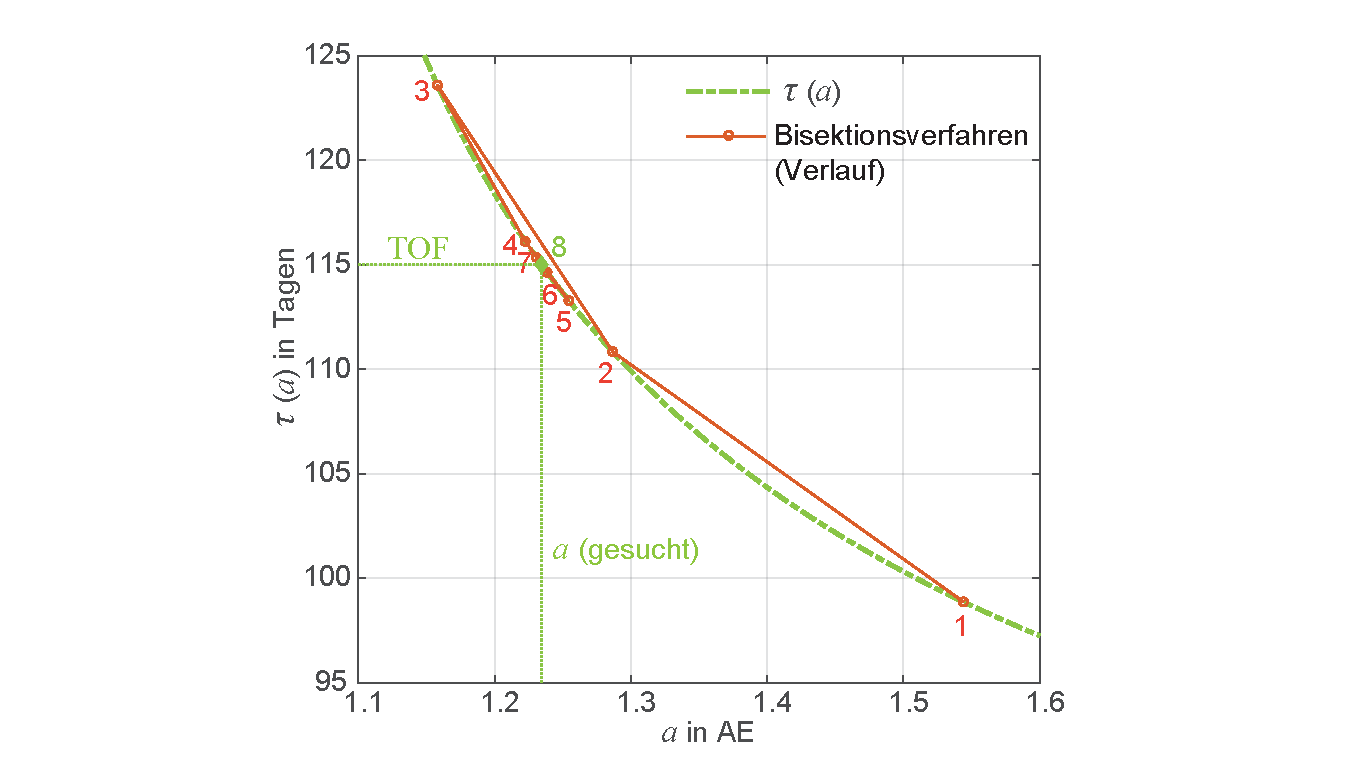
\includegraphics[width=\textwidth]{BisektionLambert.pdf} 
	\caption[Bisektionsverfahren zur L�sung des Lambert-Problems.]{Bisektionsverfahren zur L�sung des Lambert-Problems f�r folgende Parameter: $r_1 = \SI{1.000}{AE},\, r_2 = \SI{1.525}{AE},\, \gamma = 75\degree$, und einer ToF von $t_\text{F} = 115\,\mathrm{d}$. Siehe \mscr~\mladynref{LambertProblem02.m}.}
	\label{abb:adyn_lambert_lsg04}
\end{figure}

\begin{table}[ht]
\begin{center}
\begin{tabular}{L{1cm}R{1.5cm}R{1.5cm}R{1.5cm}R{2cm}R{2cm}R{1.5cm}}
    \hline
    \rule{0pt}{3pt}&&&&&& \\
      $n$ & $a_n$ & $\alpha_n$ & $\beta_n$ & $\tau(\alpha_n)$ & $\tau(\alpha_n) - \mathrm{ToF} $ & $e_n$\\
    %\rule{0pt}{3pt}&&&&&& \\
       & $\SI{}{AE}$ &&& Tage & Tage & \\
    \rule{0pt}{3pt}&&&&&& \\
    \hline
    \rule{0pt}{3pt}&&&&&& \\
 \rule{0pt}{3pt} 1    &   1.544     &   1.911    &   0.798     &   98.87      &   -16.132      &   0.387 \\
 \rule{0pt}{3pt} 2    &   1.287     &   2.214    &   0.879     &  110.83      &    -4.166      &   0.330 \\
 \rule{0pt}{3pt} 3    &   1.158     &   2.462    &   0.931     &  123.60      &     8.596      &   0.350 \\
 \rule{0pt}{3pt} 4    &   1.222     &   2.324    &   0.904     &  116.12      &     1.120      &   0.332 \\
 \rule{0pt}{3pt} 5    &   1.255     &   2.267    &   0.891     &  113.28      &    -1.723      &   0.330 \\
 \rule{0pt}{3pt} 6    &   1.238     &   2.295    &   0.898     &  114.64      &    -0.358      &   0.331 \\
 \rule{0pt}{3pt} 7    &   1.230     &   2.309    &   0.901     &  115.37      &     0.366      &   0.331 \\
 \rule{0pt}{3pt} 8    &   1.234     &   2.302    &   0.899     &  115.00      &     0.000      &   0.331 \\
    \rule{0pt}{3pt}&&&&&& \\
    \hline
\end{tabular}    
\end{center}
\caption{Bisektionsverfahren zur L�sung des Lambert-Problems. Parameter siehe Text \bzw \figref{adyn_lambert_lsg04}.}
 %f�r folgende Parameter: $r_1 = \SI{1.0}{AE},\, r_2 = \SI{1.525}{AE},\, \gamma = 75\degree$, und einer ToF von $t_\text{F} = 115 \mathrm{d}$ \bzw $t_\text{F} = 365 \mathrm{d}.$ Siehe \mscr\mladynref{LambertProblem02.m}.}
\label{tab:adyn_bisection}
\end{table}


\end{sol} 

\textcolor{blue} {$\rightarrow$ zur} \probref{adyn_manoevers4}.\\
\noindent\rule[1ex]{\textwidth}{0.5pt}  \newpage  \clearpage

%-----------------------------------------------------------------------------------------------------------

\begin{sol}{prob:adyn_manoevers5}\label{lsg:adyn_manoevers5} %�bung16
\textbf{Venus- und Mars-Fl�ge}\\

Wir bestimmen als erstes die Flugzeit f�r eine Parabell�sung von der Erdbahn (Punkt $\text{P}_1$) zur Marsbahn (Punkt $\text{P}_2$). Diese l�sst sich aus der Barker-Gleichung\index{Barker-Gleichung} \eqref{eq:hm_Barker_glg} bestimmen (siehe L�sung zu \probref{adyn_manoevers4} und\cite{Izzo2015}, \cite{sangra2021}):
			\begin{align}
								t_\text{Par} &= \frac{\sqrt{2}}{3}\,\sqrt{\frac{s^3}{\mu}}\,\lk 1-\sqrt{\lk\frac{s-c}{s}\rk^3}\rk\,.\label{eq:adyn_lsglambert21}
			\end{align}
Wir verweisen auf das \mscr~\mladynref{FlugVenusParabelbahn.m}, in welchem die Parabel-Flugbahn einer Raumsonde zur Venus
zu verschiedenen Startzeiten auf Basis der der L�sung des Lambert-Problems numerisch berechnet wird. Vorgegeben ist das Startdatum, gesucht ist das Ankunftsdatum mit dem
schnellsten Transfer unab�ngig vom notwendigen Antriebsbedarf.

\begin{figure}[H]
	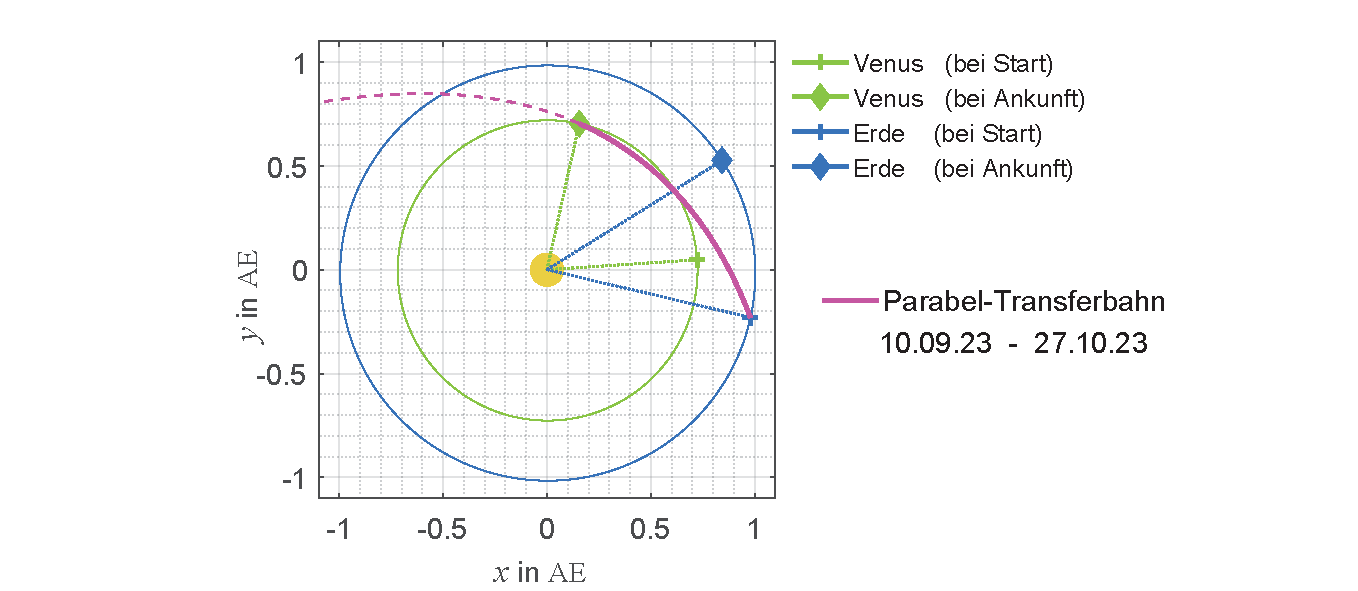
\includegraphics[width=\textwidth]{ParabelTransferVenus.pdf} 
	\caption[Parabel-L�sung des Lambert-Problems.]{Parabel-L�sung des Lambert-Problems f�r einen Flug zur Venus. Siehe \mscr~\mladynref{FlugVenusParabelbahn.m}.}
	\label{abb:adyn_lambert_lsg05}
\end{figure}

F�r die Berechnung der Transferbahn (elliptisch) von der Erde zur Venus oder zum Mars bei vorgegebener ToF benutzen wir die \mscr~\mladynref{LambertProblem03.m} \bzw \mladynref{LambertMarsVenus.m}, in welchen �ber die Routine \mladyniref{LambertSolver3.m}. die Parameter des interplanetaren Raumflugs zum Mars bzw. zur Venus �ber die L�sung des Lambert-Problems berechnet werden. Vorgegeben sind dabei die Positionsvektoren 1 und 2, sowie die Abflug und Ankunftszeit. Die Abflugs-Ankunfs-Positionen m�ssen vorher berechnet werden (z.B. �ber \mscr~\mladynref{FlugzeitenMarsVenus.m} oder �ber Programme aus dem Kapitel Himmelsmechanik, wie \mscr~\mlhmref{PlanetenbahnenKepler.m} und \mlhmref{PlanetenPositionen.m}. \\

\begin{figure}[H]
	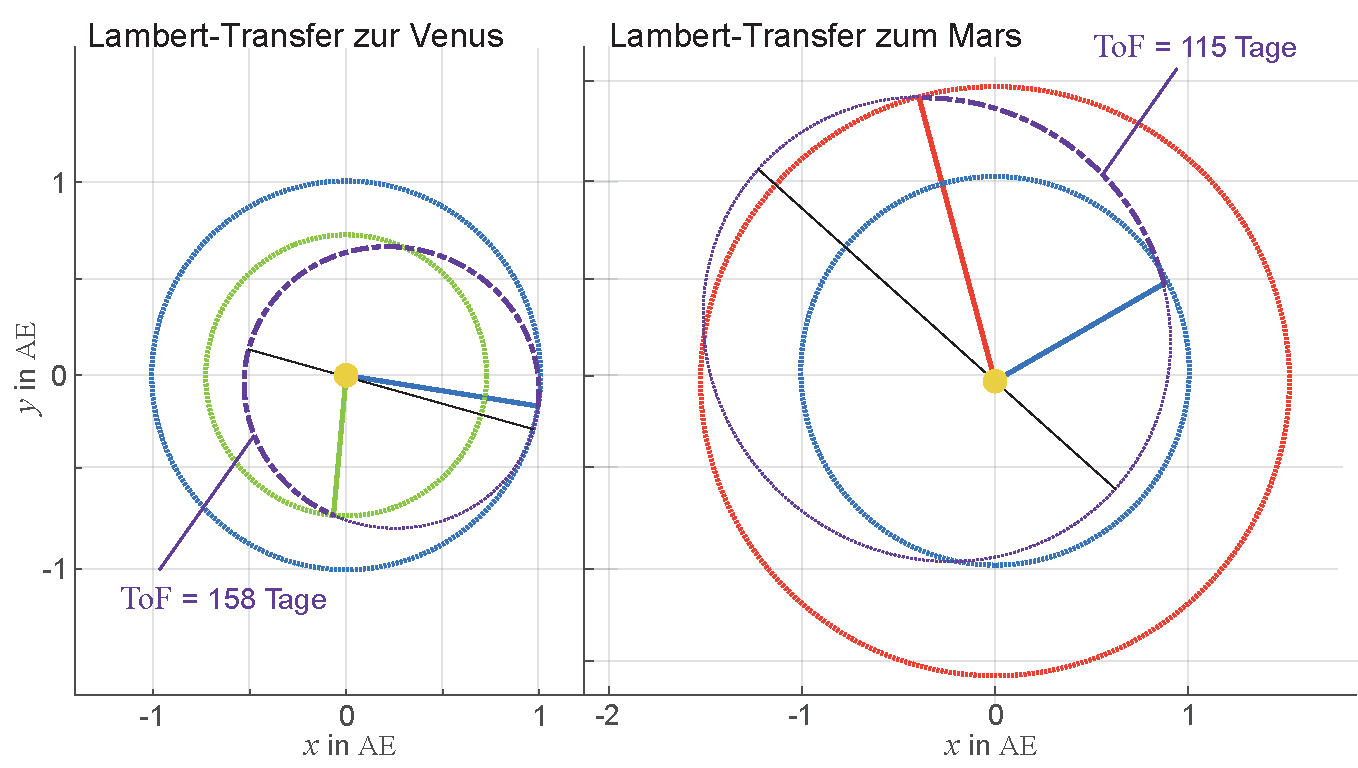
\includegraphics[width=\textwidth]{LambertTransferVenusMars.pdf} 
	\caption[L�sung des Lambert-Problems f�r Fl�ge zu Venus und Mars.]{L�sung des Lambert-Problems f�r Fl�ge zu Venus und Mars. Siehe \mscr~\mladynref{LambertProblem03.m}.}
	\label{abb:adyn_lambert_lsg06}
\end{figure}

\end{sol} 
\textcolor{blue} {$\rightarrow$ zur} \probref{adyn_manoevers5}.\\
\noindent\rule[1ex]{\textwidth}{0.5pt}  \newpage  \clearpage

%-----------------------------------------------------------------------------------------------------------

\begin{sol}{prob:adyn_manoevers6}\label{lsg:adyn_manoevers6} %�bung17
\textbf{Abfang ballistischer Raketen}\\

Die L�sung ist  im \mscr~\mladynref{LambertICBM.m} detailliert und mit ausf�hrlichen Kommentaren hinterlegt.
Die Vorgehensweise ist dabei wie folgt:
\begin{enumerate}[1.]
	\item Aus den gegebenen Werten f�r $\vec{R}$ und $\vec{V}$ der ICBM bestimmt man die Bahnparameter der ICBM. Wir verweisen auf \probref{adyn_orbits1}.
	\item Man berechnet mit diesen Bahnparametern �ber die Kepler-Gleichung \bzw die Methode mit den Gau�-Vektoren (PQR) (siehe \kap{hm_bahnen_hk_PQR}) den zeitlichen Verlauf der Trajektorie der ICBM und insbesondere den Punkt $\vec{R}(t_1+\mathrm{ToF})$, den diese nach $\mathrm{ToF}=\SI{30 }{\minute}$ errreicht. Wir erhalten:
\begin{align}
    \vec{R}(t_1+\mathrm{ToF})=[3930.7, 9762.2, 1583.3]\,\SI{}{\km}\,.
\end{align}
	\item F�r den Abf�nger gilt das Lambert-Problem mit $[\mathrm{P}_1,\mathrm{P}_2] = [\vec{r}(t_1), \vec{R}(t_1+\mathrm{ToF})]$.
	\item Man �berpr�ft, ob es �berhaupt eine L�sung geben kann. Dazu bestimmt man die minimale Flugzeit zu $t_\text{par} = \SI{16.0}{\minute}$ und die maximale Flugzeit zu $t_\text{m} = \SI{33.6}{\minute}$. Unsere $\mathrm{ToF}$ liegt dazwischen, es gibt also eine L�sung.
	\item Wir l�sen das Lambert-Problem wieder durch das in \probref{adyn_manoevers4} eingef�hrte Bisektionsverfahren und erhalten:
\begin{align}
    a=\SI{6130.7}{\km}\,,~~~\alpha = 2.9841\,,~~~\beta = 1.5418\,.
\end{align}
	\item Wir bestimmen mit diesen $a$, $\alpha$ und $\beta$ noch die notwendige Geschwindigkeit $\vec{v}_\text{trans}(t_1)$, die der Abf�nger am Punkt $\mathrm{P}_1$ haben muss, damit er auf die richtige Abfangbahn gelangt. Sie ergibt sich aus \eqref{eq:adyn_lambert08}zu:
\begin{align}
    \vec{v}_\text{trans}(t_1) &= (A+B)\,\vec{e}_c - (A-B)\,\vec{e}_1 = [2.16, 6.61, 1.13]\,\SI{}{\km\per\second}\, \\
		&\text{mit}\nonumber\\
		A &= \sqrt{\frac{G\,m_\text{E}}{4a}}\,\cot\frac{\alpha}{2}\,~~~~B = \sqrt{\frac{G\,m_\text{E}}{4a}}\,\cot\frac{\beta}{2}\,.\nonumber
\end{align}	
	\item Damit kann man sofort den erforderlichen Antriebsbedarf ermitteln, den man aufbringen muss, um den Abf�nger auf den richtigen Kurs zu bringen. Man erh�lt:
	\begin{align}
    \Delta \vec{v} &= \vec{v}_\text{trans}(t_1) - \vec{v}_1 = [4.66, 0.12,-1.37]\,\SI{}{\km\per\second}\,.		\\
		&\text{bzw}\nonumber\\
    \Delta v &= \SI{4.863}{\km\per\second}\,.
\end{align}	
	\item Zum Schlu� kann man aus $\vec{v}_\text{trans}(t_1)$ und $\vec{r}_1$ noch analog \probref{adyn_orbits1} die Bahnparameter der Abfangbahn berechnen und daraus mittels der Gau�-Vektoren-Methode (siehe \kap{hm_bahnen_hk_PQR}) die Trajektorie des Abf�ngers bestimmen, der sein Ziel nach genau 30 min erreicht (\figref{LambertAbfangICBM}).
\end{enumerate}

\begin{figure}[H]
	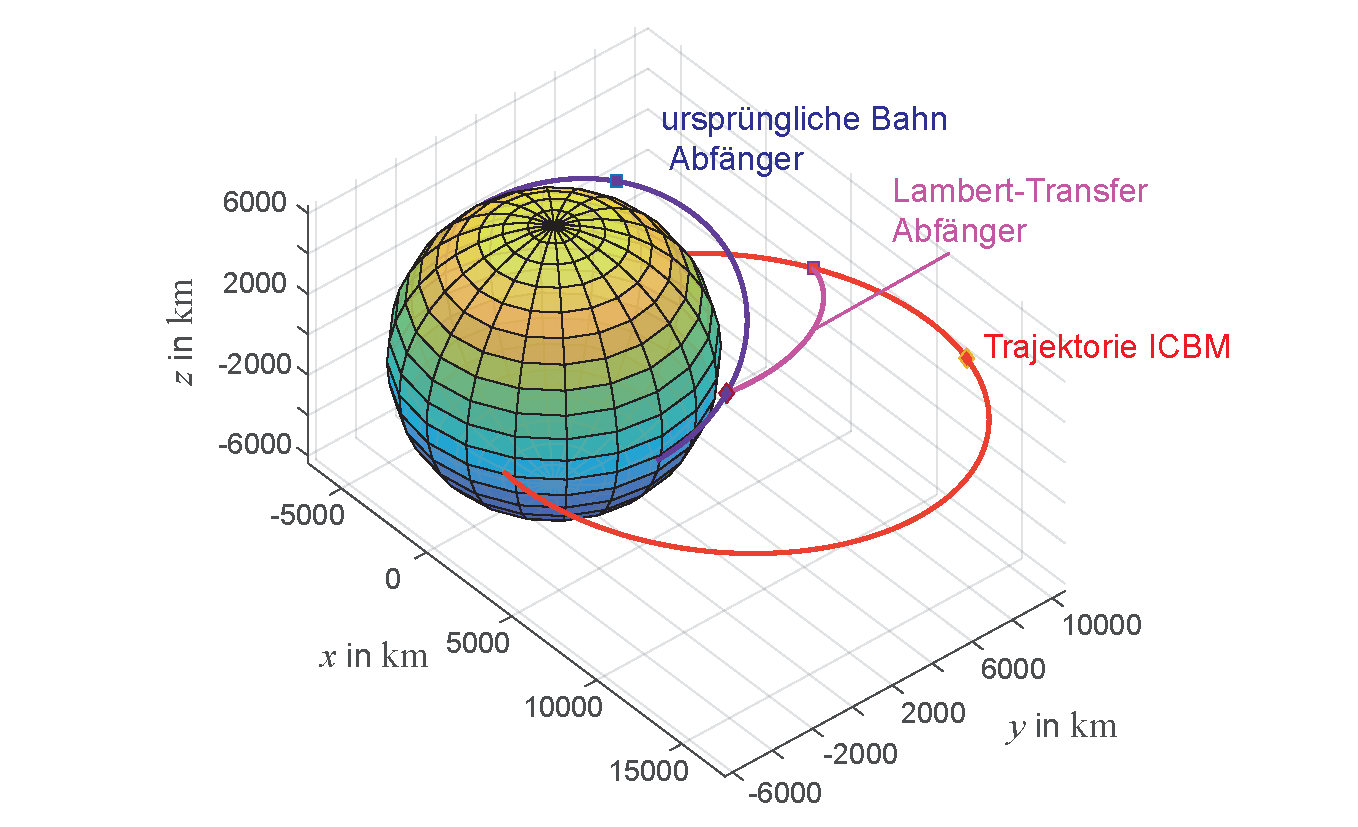
\includegraphics[width=\textwidth]{LambertAbfangICBM.pdf} 
	\caption[Abfang ballistischer Raketen.]{Abfang ballistischer Raketen. Dargestellt sind die Trajektorien der ICBM und des Abf�ngers mit und ohne $\Delta v$. Parameter siehe Text.}
	\label{abb:LambertAbfangICBM}
\end{figure}


\end{sol} 
\textcolor{blue} {$\rightarrow$ zur} \probref{adyn_manoevers6}.\\
\noindent\rule[1ex]{\textwidth}{0.5pt}  \newpage  \clearpage

%-----------------------------------------------------------------------------------------------------------

\begin{sol}{prob:adyn_manoevers7}\label{lsg:adyn_manoevers7} %�bung18
\textbf{Mondflug mit Ionenstrahltriebwerk}

\begin{itemize}
	\item
	Die Rechnungen sind im \mscr~\mladynref{Ionenantrieb02.m} ausgef�hrt und in \figref{IonenantriebExakt} dargestellt. Man sieht, dass die N�herung von \kap{adyn_kont_maneuver} zusammenbricht, wenn die Radius�nderung der Bahn per Umlauf gr��er wird.

\begin{figure}[H]
	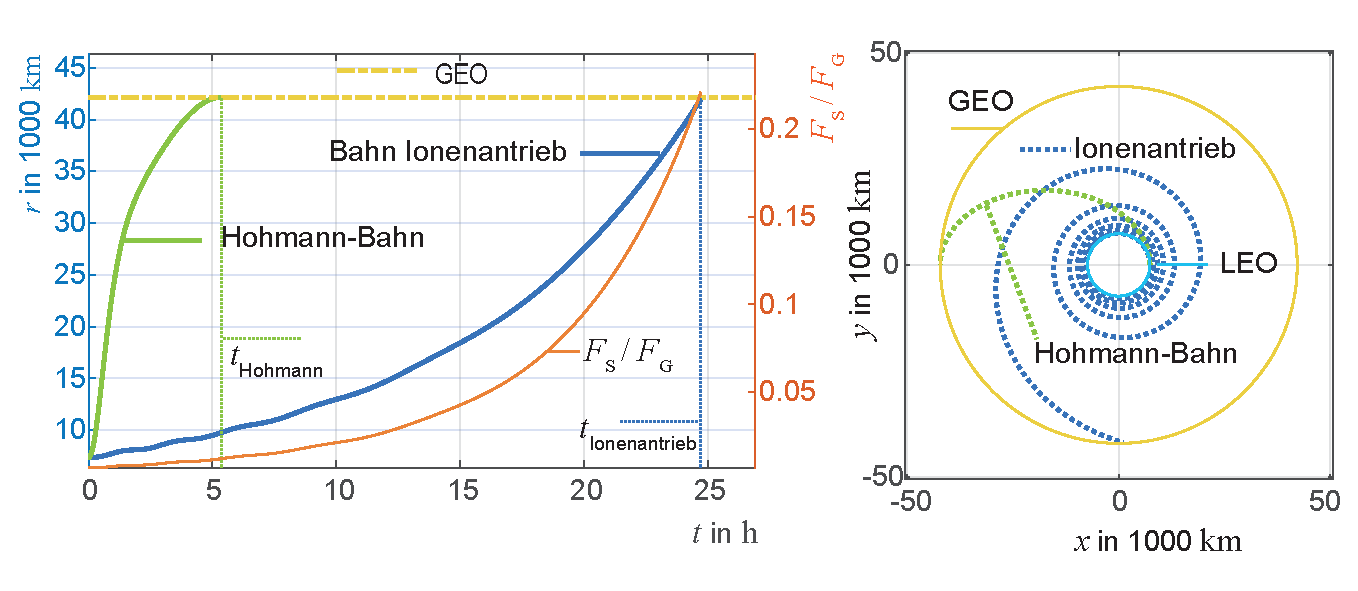
\includegraphics[width=\textwidth]{IonenantriebExakt.pdf} 
	\caption[Vergleich Hohmann-Transfer und Ionenantrieb.]{Vergleich Hohmann-Transfer und Ionenantrieb (LEO zu GEO), numerische L�sung der Bewegungsgleichung \eqref{eq:adyn_ionentr_01} f�r ein Triebwerk mit kontinuierlichem Schub. F�r den Ionenantrieb wurde ein konstanter Schub von $\SI{0.5}{\newton}$ angesetzt. Der Massenaussto� wurde bei der numerische Rechnung ber�cksichtigt.}
	\label{abb:IonenantriebExakt}
\end{figure}

	\item Die Rechnungen sind im \mscr~\mladynref{IonenantriebMond.m} ausgef�hrt. Dabei wurde die Triebwerksleistung entlang der Bahn linear so reduziert, dass sie bei der Entfernung, die dem Abstand des Lagrange-Punkts $\text{L}_1$ zwischen Erde und Mond entspricht, Null wird. Danach bewegt sich die Sonde allein im Gravitationsfeld des Mondes. Der Hohmann-Transfer wurde ebenfalls unter Ber�cksichtigung der Gravitationswirkung des Mondes berechnet.
Das Ergebnis der Rechnungen ist in der \figref{IonenantriebMoon} zu sehen.

\begin{figure}[H]
	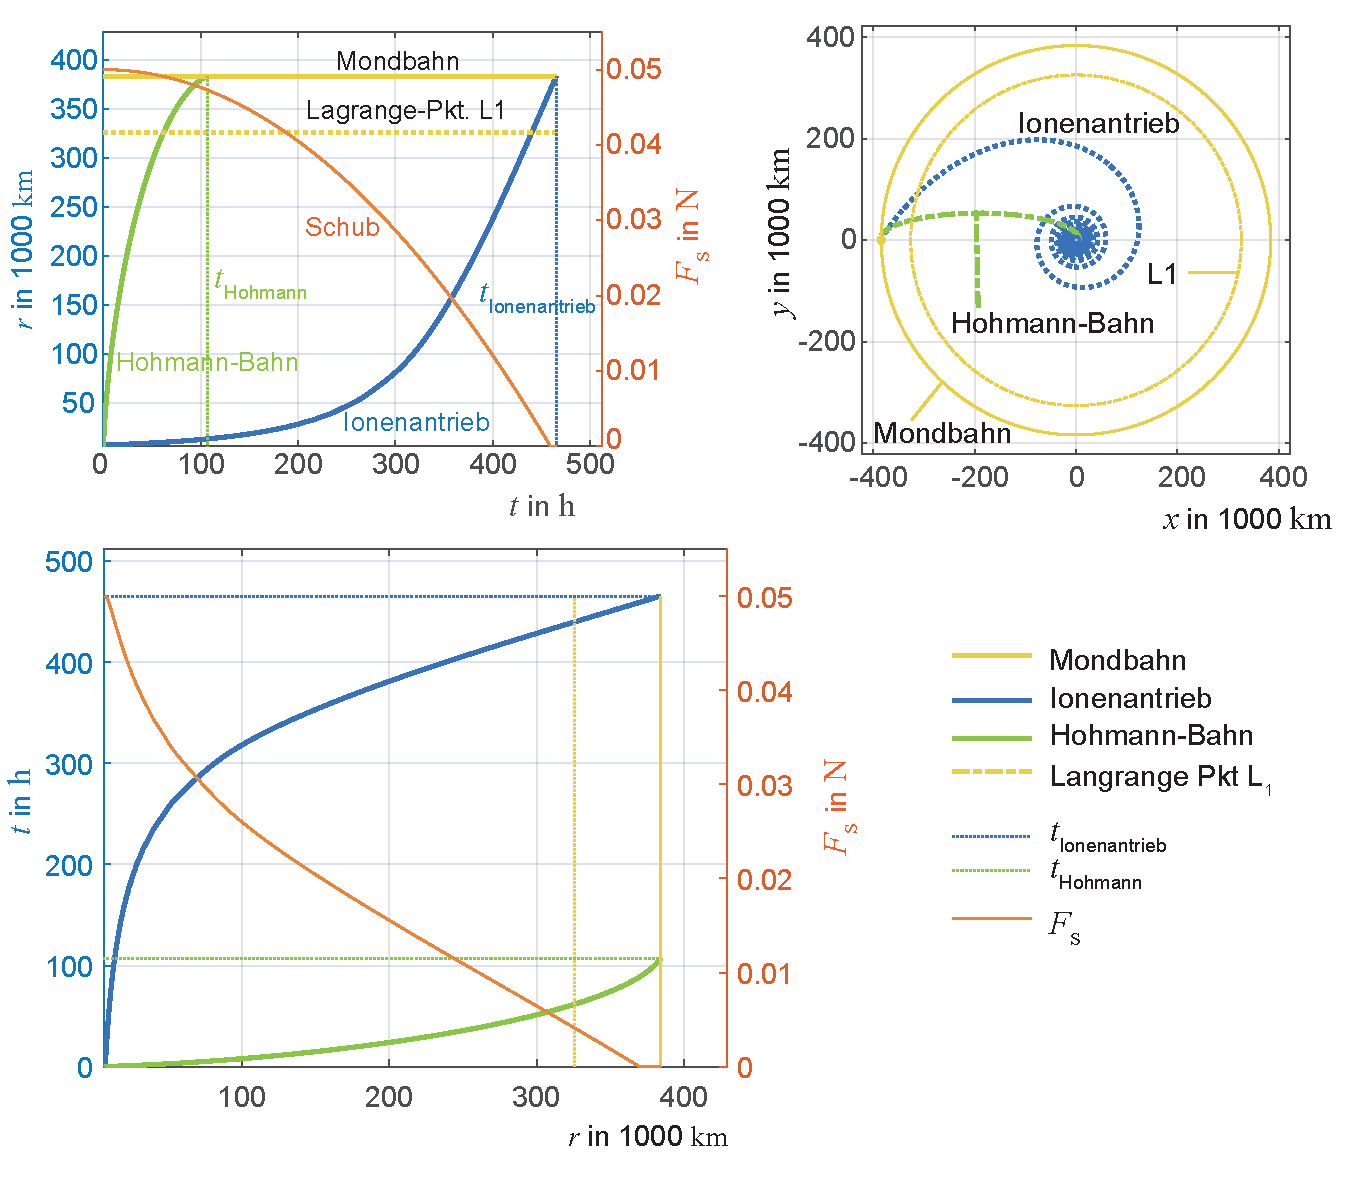
\includegraphics[width=\textwidth]{IonenantriebMoon.pdf} 
	\caption[Vergleich Hohmann-Transfer und Ionenantrieb zum Mond.]{Vergleich Hohmann-Transfer und Ionenantrieb zum Mond. F�r den Ionenantrieb wurde ein initialer Schub von $\SI{0.05}{\newton}$ der bis zum Gravitationsgleichgewicht zwischen Erde und Mond kontinuierlich reduziert wurde. Ebenso wurde der Massenaussto� bei der numerische Rechnung ber�cksichtigt.}
	\label{abb:IonenantriebMoon}
\end{figure}

\end{itemize}

\end{sol} 
\textcolor{blue} {$\rightarrow$ zur} \probref{adyn_manoevers7}.\\
\noindent\rule[1ex]{\textwidth}{0.5pt}  \newpage  \clearpage

%-----------------------------------------------------------------------------------------------------------

\begin{sol}{prob:adyn_SOI}\label{lsg:adyn_SOI} %�bung19
\textbf{Einflusssph�re - Sphere of Influence (SOI)}\\

Die Begriffe Hill-Sph�re\index{Hill-Sph�re} und Einflusssph�re\index{Einflusssph�re}\index{Sphere of Influence, SOI} adressieren zwei unterschiedliche Probleme:\\

\textit{Hill Sph�re:} Gegeben sind eine gro�e Masse $m_1$ (\zb die Sonne) und eine etwas kleinere Masse $m_2 < m_1$ (\zb die Erde) gegeben. Letztere bewegt sich um die gr��ere Masse. Es wird der Bereich gesucht, in dem f�r eine noch kleinere Masse $m_\text{M}$ (\zb der Mond) eine stabile Bahn um die kleine Masse ($m_2$) m�glich ist. Dieser Bereich wird Hill-Sph�re genannt. Die Berechnung der Hill-Sph�re hatten wir in \probref{hm_hill_sphere} ausf�hrlich behandelt und hatten dor mit $a$ als den Abstand zwischen den Massen $m_1$ und $m_2$ erhalten \eqref{eq:hm_moon_moon_lsg9}:
\begin{equation}
	r_\text{H} = a\,\sqrt[3]{\frac{1}{3}\frac{m_1}{m_2}} \,. \label{eq:adyn_hill_sphere_radius}:
\end{equation}

\textit{SOI:} Hier sind nun zwei relativ gro�e Massen $m_1, m_2$ gegeben (\zb Mars $m_1$ und Jupiter $m_2$ oder Sonne $m_2$ und Mars $m_1$ ) und eine sehr kleine Masse $m_\text{R}$ (\zb eine Raumsonde), die sich zwischen diesen beiden Massen bewegt. Es werden die Bereiche gesucht, in welchem jeweils eines der Zentren der Massen $m_1, m_2$ den Ursprung des Koordinatensystems bildet, welches f�r die Beschreibung der Bewegung der sehr kleinen Masse $m_\text{R}$  verwendet wird. In diesem Bereich muss dann f�r die Berechnung der Bewegung nur die Gravitationskraft der jeweiligen die SOI definierenden Masse $m_1$ oder $m_2$ ber�cksichtigt werden. Damit kann in der Astrodynamik bei interplanetaren Raumfl�gen die Trajektorie oft durch Aneinanderf�gen von Kepler-Bahn Abschnitten in den aufeinanderfolgenden SOI der einzelnen Planeten \bzw der Sonne (im interplanetaren Raum) n�herungsweise berechnet werden (sogenannte \textit{patched conic trajectories}.\\
Zur Herleitung der Beziehung f�r den Radius der SOI als Funktion der Massen  $m_1, m_2$ verwendet man zwei Referenzsysteme:
\begin{itemize}
	\item Zum einen erfolgt die Betrachtung der Bewegung der Raumsonde in einem Koordinaten\-system, dessen Ursprung im Zentrum der Masse $m_1$ liegt und ber�cksichtigt als Hauptwirkung nur die Gravitation der Masse $m_1$. Die Gravitationsbeschleunigung der gr��eren Masse $m_2$ wird in der Bewegungsgleichung als St�rgr��e eingef�hrt, im Prinzip als erste Abeitung.
	\item Dann betrachtet man die Bewegung der Raumsonde in dem \KOS, dessen Ursprung im Zentrum der Masse $m_2$ liegt und ber�cksichtigt als Hauptwirkung nur die Gravitation der Masse $m_2$. In der Bewegungsgleichung wird dann wiederum die Gravitationsbeschleunigung der Masse $m_1$ als St�rgr��e eingef�hrt.
\end{itemize}

\begin{figure}[H]
	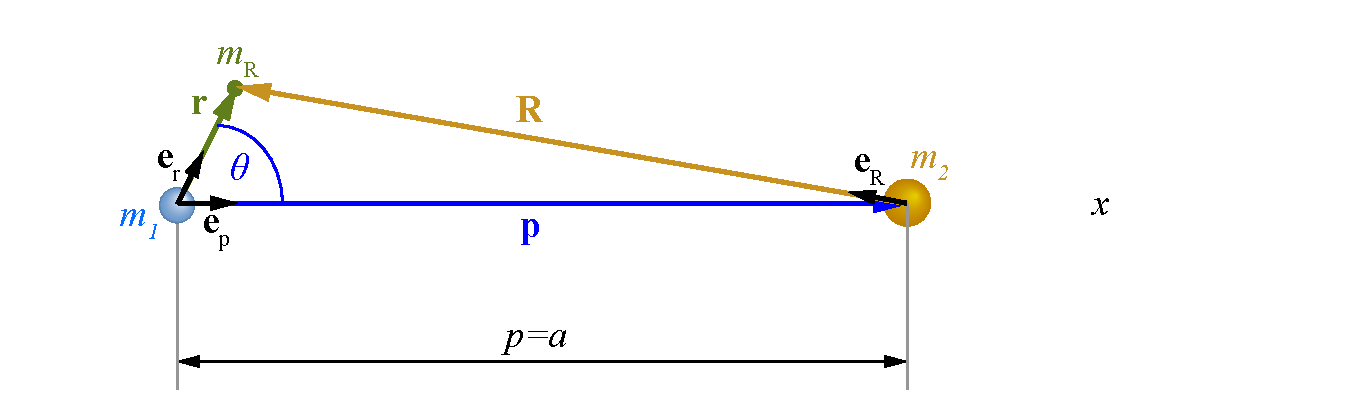
\includegraphics[width=\textwidth]{GeometrieHerleitungSOI.pdf} 
	\caption[Zur Herleitung der Einflusssph�re.]{Zur Herleitung der Einflusssph�re.}
	\label{abb:adyn_SOI01}
\end{figure}

Es ergeben sich folgende Bewegungsgleichungen (f�r $m_\text{R} \ll m_1,m_2$):\footnote{Die Herleitung wird als Zusatz�bung empfohlen, siehe auch \kap{hm_potentialtheorie} sowie \figref{adyn_SOI01}.}
\begin{subequations}
\begin{align}
    \ddot{\vec{r}} &= -G\,m_1\,\frac{\vec{r}}{r^3}-G\,m_2\,\lk\frac{\vec{p}}{p^3} + \frac{\vec{R}}{R^3}\rk\,,\\
    \ddot{\vec{R}} &= -G\,m_2\,\frac{\vec{R}}{R^3}-G\,m_1\,\lk\frac{\vec{r}}{r^3} - \frac{\vec{p}}{p^3}\rk\,.
\end{align}    \label{eq:adyn_SOI01}
\end{subequations}

Diese Gleichungen k�nnen geschrieben werden als:
\begin{subequations}
\begin{align}
     \ddot{\vec{r}} &= \vec{a}_{\text{H},1}^{\lk 1 \rk} + \vec{a}_{\text{S},2}^{\lk 1 \rk}\,, \\
     \ddot{\vec{R}} &= \vec{a}_{\text{H},2}^{\lk 2 \rk} + \vec{a}_{\text{S},1}^{\lk 2 \rk} \,,
\end{align} \label{eq:adyn_SOI02}
\end{subequations}

worin in $\vec{a}_{\text{H,S},i}^{\lk j \rk}$ der Index $j$ das KOS-System des jeweiligen Planeten bezeichnet und H und S f�r die Hauptgravitations- \bzw St�rbeschleunigung stehen. Letztere wird hervorgerufen jeweils durch die Masse $m_i$ ($i=1,2$). Die Beschleunigungen k�nnen mit den Einheitsvektoren $\vec{e}_\text{r},\, \vec{e}_\text{R}$ und $\vec{e}_\text{p}$aus \figref{adyn_SOI01} beschrieben werden durch:

\begin{subequations}
\begin{align}
   \vec{a}_{\text{H},1}^{\lk 1 \rk} &= -\frac{G\,m_1}{r^2}\,\vec{e}_\text{r}\,,\label{eq:adyn_SOI03a} \\ 
    \vec{a}_{\text{H},2}^{\lk 2 \rk} &= -\frac{G\,m_2}{R^2}\,\vec{e}_\text{R}\,, \label{eq:adyn_SOI03b} \\
    \vec{a}_{\text{S},2}^{\lk 1 \rk} &= +\,G\,\frac{m_2}{p^2}\,\sum\limits_{k=1}^\infty \lk \frac{r}{p}\rk^k\lek {\PL {k+1}}'\lk  \cos\theta\rk\,\vec{e}_\text{p} - {\PL {k}}'\lk\cos\theta\rk\,\vec{e}_\text{r} \rek\,, \label{eq:adyn_SOI03c} \\ 
    \vec{a}_{\text{S},1}^{\lk 2 \rk}&= +\,G\,\frac{m_1}{r^2}\,\lek \lk \frac{r}{p} \rk^2\,\vec{e}_\text{p} - \vec{e}_\text{r} \rek\,, \label{eq:adyn_SOI03d}
\end{align} \label{eq:adyn_SOI03}
\end{subequations}  

worin $\PL k$ die im \kap{hm_potentialtheorie} eingef�hrten Legendre-Polynome sind (\cite{Andrews2003}) und ${\PL k}'$ deren erste Ableitungen. 
Die Gleichungen sind direkt aus \eqref{eq:adyn_SOI01} ablesbar. Lediglich Gleichung \eqref{eq:adyn_SOI03b} erfordert eine Nebenrechnung. Sie ergibt sich aus der Definition der Legendre-Polynome und der Nutzung der verschiedenen Beziehungen zwischen den Ableitungen und den Rekursionsformeln (\cite{Riley2006, Andrews2003}). 
Wir bilden nun die Verh�ltnisse von Hauptbeschleunigung zu St�rbeschleunigung im jeweiligen \KOS. Wir dividieren dazu \eqref{eq:adyn_SOI03d} durch \eqref{eq:adyn_SOI03b} und finden:
\begin{align}
    \frac{ \vec{a}_\text{S1}^{\lk 2\rk}}{ \vec{a}_\text{H2}^{\lk 2\rk}} = \frac{m_1}{m_2}= \frac{1-2\,\lk\frac{r}{p}\rk\,\cos\theta + \lk\frac{r}{p}\rk^2}{\lk\frac{r}{p}\rk^2}\,\sqrt{\lek 1-2\,\lk\frac{r}{p}\rk^2\,\cos\theta + \lk\frac{r}{p}\rk^4\rek} \,.\label{eq:adyn_SOI04}
\end{align}
Analog erh�lt man durch Division von \eqref{eq:adyn_SOI03c} durch \eqref{eq:adyn_SOI03a}:
\begin{align}
    \frac{\vec{a}_{\text{S},2}^{\lk 2\rk}}{\vec{a}_{\text{H},1}^{\lk 2\rk}} = \frac{m_1}{m_2}\,\lk \frac{r}{p} \rk^3 \, \sqrt{\lek 1+3\cos^2\theta \rek} + \mathcal{O}\lk\frac{r}{p}^4\rk \,, \label{eq:adyn_SOI05}
\end{align}
wobei wir hier wegen $r \ll p$ alle Terme mit Potenzen von $\lk \frac{r}{p} \rk^n$, $n>3$ vernachl�ssigen. Die Gleichungen dr�cken das Verh�ltnis von St�rbeschleunigung zu Hauptbeschleunigung im jeweiligen Bezugssystem aus.\\
Gleichsetzen von \eqref{eq:adyn_SOI04} mit \eqref{eq:adyn_SOI05} bedeutet, dass die St�rungs- und Hauptbeschleunigungen an einem Ort im Abstand $r_\text{SOI} $ von dem jeweiligen Zentrum des \KOS im gleichen Verh�ltnis zueinander stehen. Man erh�lt dann eine diesen Abstand unter der Annahme $r/p \ll 1$: 
\begin{align}
    \frac{r_\text{SOI}}{p} &= \sqrt[5]{\frac{m_1{}^2}{m_2{}^2}}\,\underbrace{\lk 1+3\cos^2\theta\rk^{-\frac{1}{10}}}_{\leq 1.148}~~\rightarrow ~~~ \frac{r_\text{SOI}}{p} \approx \lk \frac{m_1}{m_2}\rk^{\frac{2}{5}}\,. \label{eq:adyn_SOI06}
\end{align}
Der Radius einer SOI h�ngt somit vom Abstand $p$ beider Massen und dem Verh�ltnis (hoch $2/5$) der beiden Massen ab. Tabelle \ref{tab:adyn_SOI01} zeigt die Radien der SOI der Planeten unseres Sonnensystems im Vergleich zu den Radien der Hill-Sph�re \eqref{eq:adyn_hill_sphere_radius}:
\begin{table}[ht]
		\begin{center}
    \begin{tabular}{|C{1.5cm}|C{2.75cm}|C{2.75cm}|C{2.75cm}|C{2.75cm}|}
    \hline
    \rule{0pt}{3pt}& & &&  \\
      Planet (Masse $m_1$) & Gro�e Halbachse\linebreak zur Sonne \linebreak (Masse $m_2$)\linebreak $\lk\SI{}{\km}\rk$ & Massenverh�ltnis Planet/Sonne \linebreak $m_1/m_2$& Radius der SOI \linebreak  $\lk\SI{}{\km}\rk$ \linebreak \linebreak \eqref{eq:adyn_SOI_radius} &  Radius der Hill-Sph�re  \linebreak  $\lk\SI{}{\km}\rk$ \linebreak \linebreak \eqref{eq:adyn_hill_sphere_radius} \\
    \rule{0pt}{3pt}&& &&  \\
    \hline
    \rule{0pt}{3pt}&& &&   \\
    \rule{0pt}{6pt} Merkur &\SI{57.9e6}{}&$\SI{0.166e-6}{}$ & $\SI{112000e06}{}$& $\SI{2.206e05}{}$\\
    \rule{0pt}{3pt}&& &&   \\
    \rule{0pt}{6pt} Venus &\SI{108.2e6}{}&$\SI{2.450e-6}{}$ & $\SI{616350e06}{}$& $\SI{1.010e+06}{}$\\
    \rule{0pt}{3pt}&& &&   \\
    \rule{0pt}{6pt} Erde & \SI{149.6e6}{}&$\SI{3.002e-6}{}$ & $\SI{924510e06}{}$& $\SI{1.496e+06}{}$\\
    \rule{0pt}{3pt}&& &&   \\
    \rule{0pt}{6pt} Mars &\SI{227.9e6}{}&$\SI{0.323e-6}{}$ & $\SI{577230e06}{}$& $\SI{1.084e+06}{}$\\
    \rule{0pt}{3pt}&& &&   \\
    \rule{0pt}{6pt} Jupiter &\SI{778.6e6}{}&$\SI{954.490e-6}{}$ & $\SI{48219000e06}{}$& $\SI{5.315e+07}{}$\\
    \rule{0pt}{3pt}&& &&   \\
    \rule{0pt}{6pt} Saturn &\SI{1433.5e6}{}&$\SI{285.641e-6}{}$ & $\SI{54793000e06}{}$& $\SI{6.546e+07}{}$\\
    \rule{0pt}{3pt}&& &&   \\
    \rule{0pt}{6pt} Uranus &\SI{2872.5e6}{}&$\SI{43.651e-6}{}$ & $\SI{51791000e06}{}$& $\SI{7.013e+07}{}$\\
    \rule{0pt}{3pt}&& &&   \\
    \rule{0pt}{6pt} Neptun &\SI{4495.1e6}{}&$\SI{51.295e-6}{}$ & $\SI{86451000e06}{}$& $\SI{1.158e+08}{}$\\
    \rule{0pt}{3pt}&& &&   \\
    \hline
    \end{tabular} 
		\end{center}
		\caption{Vergleich Radien der SOI mit dem Hill-Sph�re f�r die Planeten unseres Sonnensystems.}
		\label{tab:adyn_SOI01}
\end{table}

Im letzten Schritt in \eqref{eq:adyn_SOI06} haben wir die $\theta$-Abh�ngigkeit vernachl�ssigt. Ber�cksichtigt man diese, so ergibt sich ein oblater Sph�roid anstelle einer Einflusssph�re (Sphere of Influence). In den meisten F�llen reicht die Kugelbetrachtung aber aus, man kann also schreiben:
\begin{align}
	r_\text{SOI} = a\,\sqrt[5]{\lk \frac{m_1}{m_2}\rk^2} \,, \label{eq:adyn_SOI_radius}
\end{align}
worin a der Abstand zwischen den beiden Massen (\ia gleich der gro�en Halbachse von $m_1$ um $m_2$) ist.\\
Man wird also immer dann, wenn sich die Raumsonde in geringerem Abstand als $r_\text{SOI}$  von der Masse $m_1$ befindet, die Bewegung als Zweik�rperproblem mit den Massen $m_1,\,m_\text{R}$ behandeln k�nnen, bei Abst�nden gr��er als $r_\text{SOI}$ als Zweik�rperproblem mit den Massen $m_2,\,m_\text{R}$.\\

\end{sol} 
\textcolor{blue} {$\rightarrow$ zur} \probref{adyn_SOI}.\\
\noindent\rule[1ex]{\textwidth}{0.5pt}  \newpage  \clearpage

%-----------------------------------------------------------------------------------------------------------

\begin{sol}{prob:adyn_swingby01}\label{lsg:adyn_swingby01} %�bung20
\textbf{Gravity-Assist-Man�ver - Analytische L�sung}\\

Wir beginnen mit:
\begin{subequations}
\begin{align}
        \vec{v}_1{}' &= \vec{v}_1 - \vec{v}_\text{P} \,, \label{eq:adyn_lsgswingby01a} \\
        v_1{}'^2     &= v_1{}^2 + v_\text{P}{}^2 - 2\,v_1{}'\,v_\text{P}\,\cos\gamma_1{}'\,, \label{eq:adyn_lsgswingby01b} \\
        \vec{v}_2{}  &= \vec{v}_2{}' + \vec{v}_\text{P} \,, \label{eq:adyn_lsgswingby02a} \\
        v_2{}^2      &= v_2{}'^2 + v_\text{P}{}^2 + 2\,v_2{}'\,v_\text{P}\,\cos\beta_2{}' \,, \label{eq:adyn_lsgswingby02b} \\
        v_1{}'       &= v_2{}'= v_\infty \,. \label{eq:adyn_lsgswingby02c} 
\end{align} %\label{eq:adyn_lsgswingby02} 
\end{subequations}
F�r die weitere numerische Auswertung lassen sich aus \eqref{eq:adyn_swingby01}, \eqref{eq:adyn_swingby03} und \figref{adyn_swingby01} durch Anwendung des Kosinussatzes \bzw geometrische �berlegungen aus der Streuhyperbel noch einige n�tzliche Beziehungen, \zb zwischen dem Winkel $\beta_2{}'$ und dem Streuwinkel $\vartheta'$ sowie f�r den Winkel $\varphi'$ gewinnen:
\begin{subequations}
\begin{align}
        \beta_2{}' &= \beta_1{}' -\vartheta' = \beta_1{}' + 2\varphi' - 180\degree \label{eq:adyn_lsgswingby03a} \\
        \cos\beta_2{}' &= \cos\,\beta_1{}'\,\lk 1-2\cos^2\varphi'\rk + 2\cos\varphi'\,\sqrt{1-\cos^2\varphi'}\,\sqrt{1-\beta_1'{}^2} \label{eq:adyn_lsgswingby03b} \\
        \cos\beta_1{}' &= \frac{{v_1{}}^2+v_\text{P}{}^2-{v_1{}'}^2}{2\,v_1\,v_\text{P}} \label{eq:adyn_lsgswingby03c}
\end{align}%\label{eq:adyn_lsgswingby03} 
\end{subequations}
Die Gr��e $\cos\varphi'$ k�nnen wir ebenfalls aus \figref{adyn_swingby01} mit der Hyperbelgleichung durch
\begin{align}
    \cos\varphi' &= \frac{1}{1+ (r_\text{per}\,v_1{}'^2)/(G\,m_\text{P})} = -\frac{1}{e}\,\label{eq:adyn_lsgswingby04} 
\end{align}
ausdr�cken.

\begin{nebenrechnungNeu} {} \\
Der Winkel $\varphi'$ h�ngt mit dem asymptotischen Grenzwinkel $\theta_\infty{}'$ der Hyperbel wie folgt zusammen:
\begin{align}
    \theta_\infty{}' = -\frac{1}{e} = + \cos\lk 180\degree-\varphi'\rk = - \cos\varphi' \label{eq:adyn_lsgswingby05} 
\end{align}
Die Exzentrizit�t ist nach \eqref{eq:hm_relations2} gegeben durch
\begin{align}
    e= \sqrt{1+\frac{2\,H\,L^2}{\mu_\text{P}{}^2}} = \sqrt{1+\frac{2L^2}{\mu_\text{P}{}^2}\,\frac{v_1{}'^2}{2}} = \sqrt{1 + \frac{b^2\,v_1{}'^4}{\mu_\text{P}^2}}\,, \label{eq:adyn_lsgswingby06} 
\end{align}
wobei wir $H = v_1{}'^2/2$ f�r $r\to \infty$ und $L_\infty = b\,v_1{}' = b\,v_2{}' = b\, v_\infty$ f�r $r\to \infty$ benutzt haben.\\
Wegen der Drehimpulserhaltung k�nnen wir $L_\infty$ durch $L_\text{per} = r_\text{per}\,v_\text{per}{}'$ am Perizentrum ersetzen und benutzen dabei den \textit{vis-viva}-Satz \eqref{eq:hm_vis-viva}, womit wir erhalten:
\begin{align}
    L = b\,v_1{}' = r_\text{per}\,v_\text{per}{}'~~~\text{und}~~~
    \frac{v_1{}'}{2}^2 = \frac{v_\text{per}{}'^2}{2} - \frac{\mu_\text{P}}{r_\text{per}}\,.\label{eq:adyn_lsgswingby07} 
\end{align}
\end{nebenrechnungNeu}

\newpage
Mit den Beziehungen in \eqref{eq:adyn_lsgswingby07} k�nnen wir in \eqref{eq:adyn_lsgswingby06} den Streuparameter $b$ eliminieren und erhalten aus \eqref{eq:adyn_lsgswingby02b} mit \eqref{eq:adyn_lsgswingby05} �ber \eqref{eq:adyn_lsgswingby03b} schlie�lich die heliozentrische Geschwindigkeit des Raumschiffs $v_2$ beim Verlassen der Einflusssph�re des Gravity-Assist-Planeten am Punkt $\text{P}_2$:
\begin{subequations}
    \begin{align}
        v_2{}^2 = v_1{}^2 - \frac{2\,C_1}{C_2{}^2} + \frac{4\,v_1{}'\,v_\text{P}}{C_2}\,\sqrt{1-\frac{1}{C_2{}^2}}\,\sqrt{1-\lk\frac{C_1}{2\,v_1{}'\,v_\text{P}}\rk^2}\label{eq:adyn_lsgswingby08a}
    \end{align}
    mit 
    \begin{align}
        C_1 &= v_1{}^2 - v_\text{P}^2 - v_1{}'^2 \label{eq:adyn_lsgswingby08b}\,,\\
        C_2 &= 1+\frac{r_\text{per}}{\mu_\text{P}}\,v_1{}'{}^2 \label{eq:adyn_lsgswingby08c}\,,\\
        v_1{}'&= \sqrt{v_1{}^2 +v_\text{P}{}^2 - 2\,v_1\,v_\text{P}\,\cos\gamma_1}\,.\label{eq:adyn_lsgswingby08d}
    \end{align}%\label{eq:adyn_lsgswingby08}
\end{subequations}
Wir haben $v_2(r_\text{per},\gamma_1)$ in \figref{adyn_lsgswingby01} dargestellt.

\begin{figure}[H]
	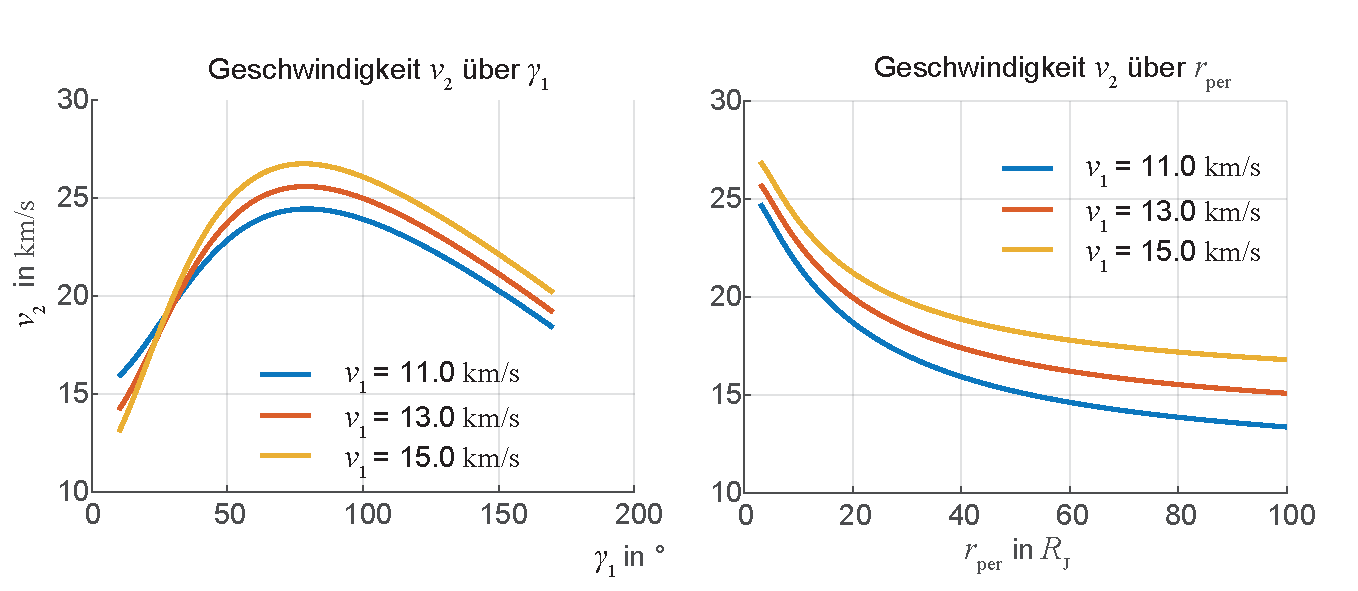
\includegraphics[width=\textwidth]{GravityAssistAnalytisch.pdf} 
	\caption[Gravity-Assist-Man�ver (Analytisch L�sung).]{Gravity-Assist-Man�ver (Analytisch L�sung).}
	\label{abb:adyn_lsgswingby01}
\end{figure}

Zum Schluss wollen wir noch den maximal m�glichen Energiegewinn bei einem Gravity-Assist-Man�ver berechnen. Dieser ergibt sich zu
\begin{align}
    \Delta H &= \frac{1}{2}\,v_2{}^2 - \frac{m_\text{S}\,G}{r_1-r_\text{per}} - \lk \frac{1}{2}\,v_1{}^2 - \frac{m_\text{S}\,G}{r_1-r_\text{per}}\rk \approx \frac{1}{2}\,\lk v_2{}^2 - v_1{}^2\rk \,.\label{eq:adyn_lsgswingby09}
\end{align}
Der Energiegewinn h�ngt also bei vorgegebenen $r_\text{per}$ von zwei Parametern ab:\\
$v_1{}'$ (\bzw. $v_1$)\, und $\beta_1{}'$ (\bzw $\gamma_1$).
Tr�gt man $\Delta H$ �ber $\beta_1{}'$ und $v_1{}'$ auf, so findet man ein Maximum bei $\beta_1{}' = 2\pi/3=120\degree$ und 
	\[v_1{}' = \sqrt{\frac{\mu_\text{P}}{r_\text{per}}}\,,
\]
Damit kann man mit den bekannten Gr��en $m_\text{P}$, $r_\text{per}$ (wir nehmen $r_\text{per} \approx 5\,R_\text{P}$ an) und $v_\text{P}$ die notwendig Anfluggeschwindigkeit $v_\text{1,opt}$ bestimmt, die den maximalen Energiegewinn bringt. Die Rechnungen sind im Detail \mscr{} \mladynref{GravityAssistAnalytik.m} ausgef�hrt. 

Der Energiegewinn $\Delta H(v_1{}', \beta_1{}')$ \bzw $\Delta H(v_1{}, \gamma_1{})$ ist in \figref{adyn_lsgswingby02a} dargestellt:

\begin{figure}[H]
	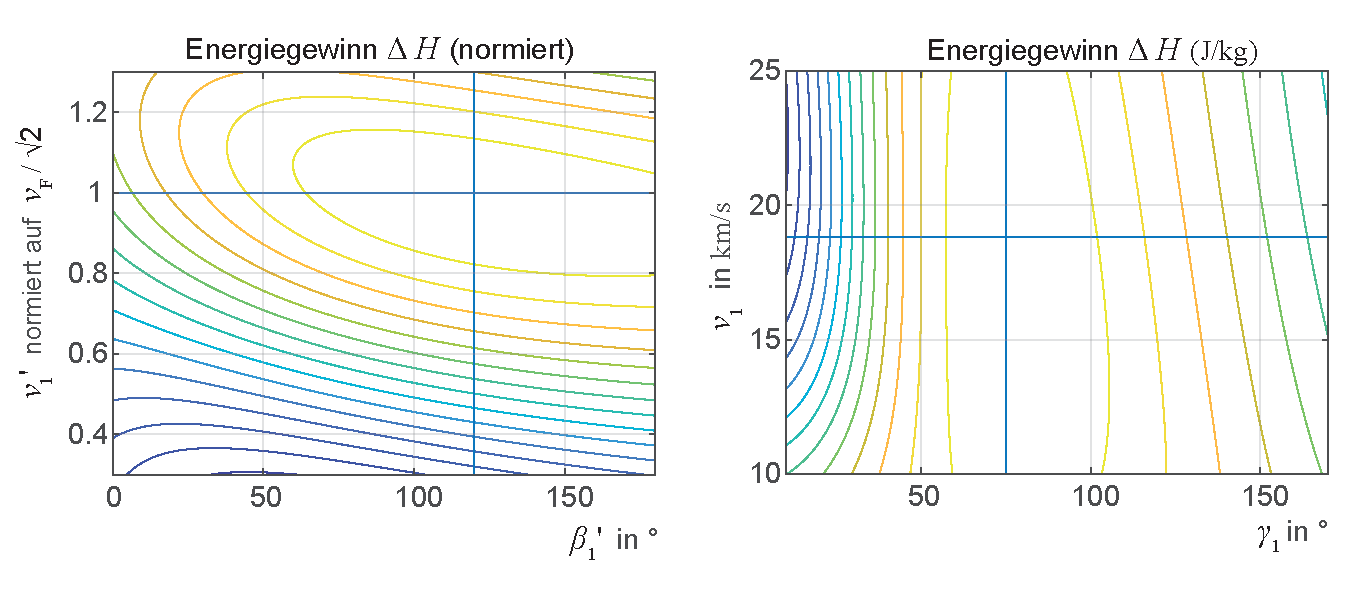
\includegraphics[width=\textwidth]{GravityAssistEnergiegewinn.pdf} 
	\caption[Gravity-Assist-Man�ver - Energiegewinn.]{Gravity-Assist-Man�ver - Energiegewinn am Beispiel des Flugs einer Raumsonde um den Jupiter.  Parameter: $r>_\text{per} = 5\,R_\text{J}$.}
	\label{abb:adyn_lsgswingby02a}
\end{figure}

\end{sol} 
\textcolor{blue} {$\rightarrow$ zur} \probref{adyn_swingby01}.\\
\noindent\rule[1ex]{\textwidth}{0.5pt}  \newpage  \clearpage
%
%%-----------------------------------------------------------------------------------------------------------

\begin{sol}{prob:adyn_swingby03}\label{lsg:adyn_swingby03} %�bung21
\textbf{Gravity-Assist-Man�ver - Simulation}\\

Die Simulation des Swing-By ist im \mscr{} \mladynref{GravityAssistSimulation.m} ausgef�hrt, die Resultate f�r ein Beispiel am Jupiter in \figref{adyn_lsgswingby02}.\\

\begin{figure}[H]
	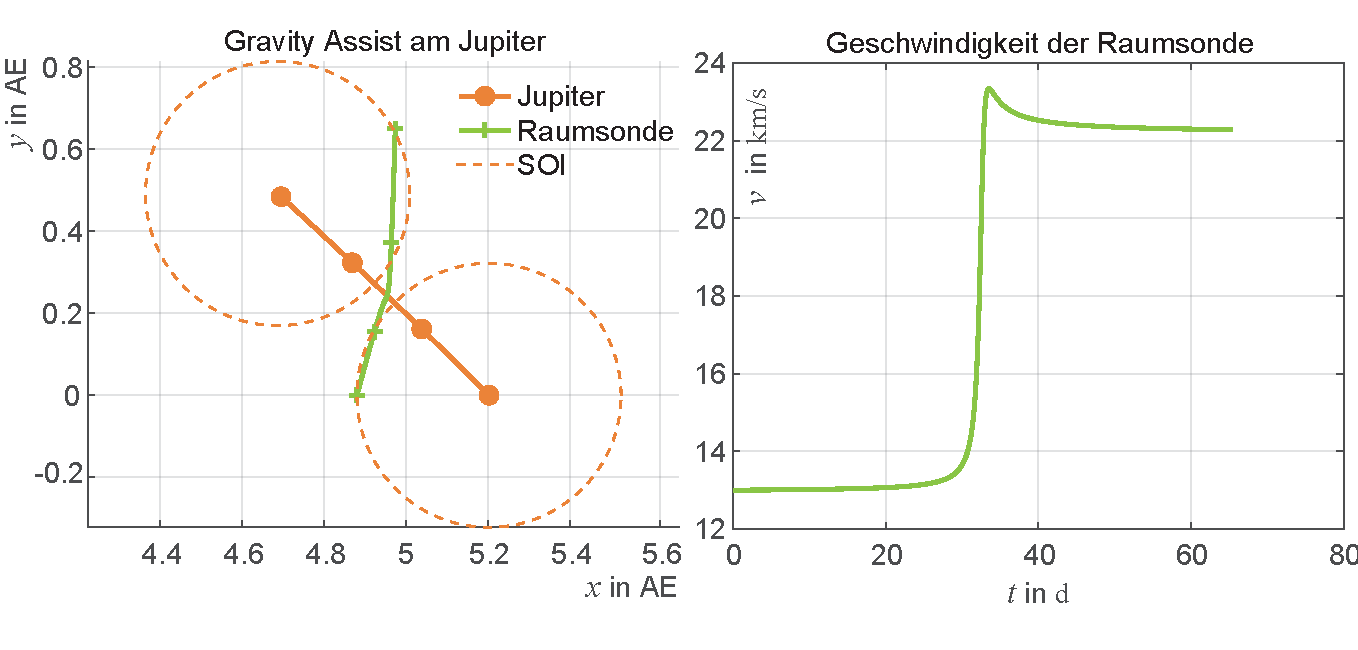
\includegraphics[width=\textwidth]{GravityAssistSimulation.pdf} 
	\caption[Gravity-Assist-Man�ver Simulation.]{Ergebnisse der Gravity-Assist-Man�ver Simulation im heliozentrischen \KOS am Beispiel des Flugs einer Raumsonde um den Jupiter.  Parameter: $v_1 = \SI{13.0}{\km\per\second}$, $\gamma_1 = 75\degree$.}
	\label{abb:adyn_lsgswingby02}
\end{figure}

\end{sol} 
\textcolor{blue} {$\rightarrow$ zur} \probref{adyn_swingby03}.\\
\noindent\rule[1ex]{\textwidth}{0.5pt}  \newpage  \clearpage

%-----------------------------------------------------------------------------------------------------------
\newpage 
\subsection{�bungen zu Rendezvous im Weltall}

\begin{sol}{prob:adyn_rendezvous01}\label{lsg:adyn_rendezvous01} %�bung22
\textbf{Rendezvous ISS und Raumtransporter}\\

Wir wollen zun�chst die Beziehungen \eqref{eq:adyn_rendez23} und \eqref{eq:adyn_rendez24} aus \kap{adyn_rendezvous} herleiten, die wir f�r unsere \matlab-
Programmierung gut verweenden k�nnen. Wir starten von der Darstellung \eqref{eq:adyn_rendez23}:
\begin{nebenrechnungNeu} {Clohessy-Wiltshire-Gleichungen}
\begin{align}
\begin{split}
    \omega\,x &= \lk 6 \omega\, y_0 + 4\dot{x}_0\rk\,  \sin \omega t + 2 \dot{y}_0 \, \cos \omega t + \omega t \, \lk -6 \omega\,  y_0 - 3 \dot{x}_0\rk  + \omega\,  \lk x_0 - 2 \dot{y}_0\rk\,,  \\
    \omega \, y &= \lk \dot{y}_0\rk \,  \sin \omega t + \lk -3 \omega \, y_0 - 2 \dot{x}_0\rk \,  \cos \omega t + \omega \, \lk 4 y_0 + 2 \dot{x}_0\rk  \, ,\\
    \omega \, z &= \dot{z}_0\, \sin \omega t + \omega\,  z_0 \, \cos \omega t +0
\end{split}\label{eq:adyn_CWEq_01}
\end{align}

Umordnung nach $\dot{x}_0, \dot{y}_0, \dot{z}_0$ und $x = y = z = 0$:

\begin{align}
\begin{split}
    \begin{pmatrix} 0 \\ 0 \\ 0 \end{pmatrix} =\,
    &\underbrace{\begin{pmatrix} 4 \sin \omega t - 3 \omega t & 2 \cos \omega t - 2 & 0 \\
    -2 \cos \omega t + 2 & \sin \omega t & 0 \\
    0 & 0 & \sin \omega t 
    \end{pmatrix} }_{\substack{\hat{A}}}
    \begin{pmatrix} \dot{x}_0 \\ \dot{y}_0 \\ \dot{z}_0 \end{pmatrix} 
    \\ &+ \underbrace{\begin{pmatrix} 6 \omega \,y_0\, \sin \omega t - 6 \omega^2 t\,y_0 + \omega x_0 \\
    -3 \omega \,y_0\, \cos \omega t + 4 \omega\, y_0 \\
    \omega\, z_0\, \cos \omega t 
    \end{pmatrix}}_{\substack{-\hat{B}}}
\end{split}\label{eq:adyn_CWEq_02}
\end{align}
\begin{align}
    -\hat{B} &= \omega \, 
    \begin{pmatrix}
        6 y_0\,\sin \omega t - 6 \omega t \,y_0 + x_0 \\ 
        -3 y_0\, \cos \omega t + 4 y_0 \\ 
        z_0\, \cos \omega t 
    \end{pmatrix} \label{eq:adyn_CWEq_03}\\
    \rightarrow \quad \hat{B} &= \omega \,
    \begin{pmatrix}
        -6 y_0 \,\sin \omega t + 6 \omega t\, y_0 - x_0 \\ 
        3 y_0\, \cos \omega t - 4 y_0 \\ 
        -z_0\, \cos \omega t 
    \end{pmatrix} \label{eq:adyn_CWEq_04}\\
  \rightarrow\quad  \hat{B} &=      \hat{A} \hat{X}\nonumber\\
    \rightarrow\quad \hat{X} &= 
    \begin{pmatrix} 
        \dot{x}_0 \\ 
        \dot{y}_0 \\ 
        \dot{z}_0 
    \end{pmatrix} 
    = \hat{A}^{-1}\, B\label{eq:adyn_CWEq_05}
\end{align}
\subsubsection*{Cramersche Regel}
\begin{align}
    \dot{x}_0 &= \frac{\det \hat{A}_x}{\det \hat{A}}, \quad
    \dot{y}_0 = \frac{\det \hat{A}_y}{\det \hat{A}}, \quad
    \dot{z}_0 = \frac{\det \hat{A}_z}{\det \hat{A}}\label{eq:adyn_CWEq_06}
\end{align}
\begin{align}
    \det \hat{A} &= 
    \begin{vmatrix}
        \lk 4 \sin \omega t - 3 \omega t \rk & -2\, \lk 1 - \cos \omega t \rk & 0 \\
        +2 \,\lk 1 - \cos \omega t \rk & \sin \omega t & 0 \\
        0 & 0 & \sin \omega t
    \end{vmatrix} \label{eq:adyn_CWEq_07}
\end{align}
\begin{align*}
    &= \lk 4 \sin \omega t - 3 \omega t \rk\, \sin^2 \omega t + 4 \sin \omega t \,\lk 1 - \cos \omega t \rk^2\\
    &= \sin \omega t \,
    \lk 4 \sin^2 \omega t - 3 \omega t \,\sin \omega t + 4 + 4 \cos^2 \omega t - 8 \cos \omega t \rk\\
    &= \sin \omega t \,
    \lek 8 \,\lk 1 - \cos \omega t \rk - 3 \omega t\, \sin \omega t \rek
\end{align*}
\begin{align}
    \det \hat{A}_z &=
    \begin{vmatrix}
         4 \sin \omega t - 3 \omega t & -2 \,\lk 1 - \cos \omega t \rk & -6 \omega \,y_0\, \sin \omega t + 6 \omega^2 t\, y_0 - \omega \,x_0 \\
        2 \,\lk 1 - \cos \omega t \rk & \sin \omega t & -3 \omega \,y_0\, \cos \omega t - 4 \omega \,y_0 \\
        0 & 0 & -\omega \,z_0\, \cos \omega t
    \end{vmatrix}\\
    &= -\lk 4 \sin \omega t - 3 \omega t \rk \,\sin \omega t \,\omega \,z_0 \,\cos \omega t - 4 \omega \,z_0 \,\cos \omega t \,\lk 1 - \cos \omega t \rk^2\nonumber\\
    &= -\cos \omega t \,\omega \,z_0 \,
    \lk 4 \sin^2 \omega t - 3 \omega t \,\sin \omega t + 4 + 4 \cos^2 \omega t - 8 \cos \omega t \rk \nonumber\\
    &= -\cos \omega t \,\omega \,z_0 \,
    \lek 8 \,\lk 1 - \cos \omega t \rk - 3 \omega t \,\sin \omega t \rek \nonumber\\
    \rightarrow \quad \dot{z}_0 &= - \frac{\cos \omega t\, \omega\, z_0}{\sin\omega t} = -\frac{\omega\,z_0}{\tan\omega t}\label{eq:adyn_CWEq_09}
\end{align}
\begin{align}
    \det \hat{A}_x &=
    \begin{vmatrix}
        6 \omega \,y_0\, \sin \omega t - 6 \omega^2 \,t \,y_0 + \omega \,x_0 & -2 \,\lk 1 - \cos \omega t \rk & 0 \\
        -3 \omega\, y_0\, \cos \omega t + 4 \omega\, y_0 & \sin \omega t & 0 \\
        \omega\, z_0\, \cos \omega t & 0 & \sin \omega t
    \end{vmatrix}\label{eq:adyn_CWEq_10}
\end{align}
\medskip

\end{nebenrechnungNeu}
%%%%%%%%%%%%%%%%%%%%%%%%%%%%%%%%%%%%%%%%%%%%%%%%%%%%%%%%%%%%%%%%%%%%%%%%%%%%%%%%%%%%%%%%%%%
%
%%BEISPIEL 1 %%%%%%%%%%%%%%%%%%%%%%%%%%%%%%%%%%%%%%%%%%%%%%%%%%%%%%%%%%%%%%%%%%%%%%%%%%%%%%%%%
%\begin{example}{R�ckkehr eines Astronauten zur Raumstation}  
%Wir nehmen folgende Parameter an: 
%\begin{align*}
    %h_\text{ISS} &= \SI{420.0}{\km}\,, ~ R_0 = \SI{6778}{\km} \,,~
    %T_\text{P}   = \SI{ 92.4}{\min}\,, ~ \omega_0 = \SI{1.13e-3}{\radian\per\second}\,,~  x_0' = y_0' = \SI{100}{\metre}\,, ~\dot{x}_0' = \dot{y}_0' = 0\,.
%\end{align*}
%\begin{enumerate}
    %\item [a)]
    %Was passiert, wenn der Astronaut \anf{nichts} macht?
    %\begin{align}
        %x'\lk t\rk &= x_0'-6\,y_0'\,\lek\omega_0 t - \sin\lk\omega_0 t\rk\rek\,, ~~~ y'\lk t\rk = y_0' +3\,y_0'\,\lek 1-\cos\lk\omega_0t\rk\rek\,. \label{eq:adyn_rendez26}
    %\end{align}
    %Der Astronaut wird sich durch die Gezeitenkraft in $x'$-Richtung immer weiter von der ISS entfernen und dabei durch die Coriolis-Kraft in $y'$-Richtung eine Art schwingende Bewegung ausf�hren (\figref{adyn_rendezvous02}).
		%
	%\begin{figure}[H]
	%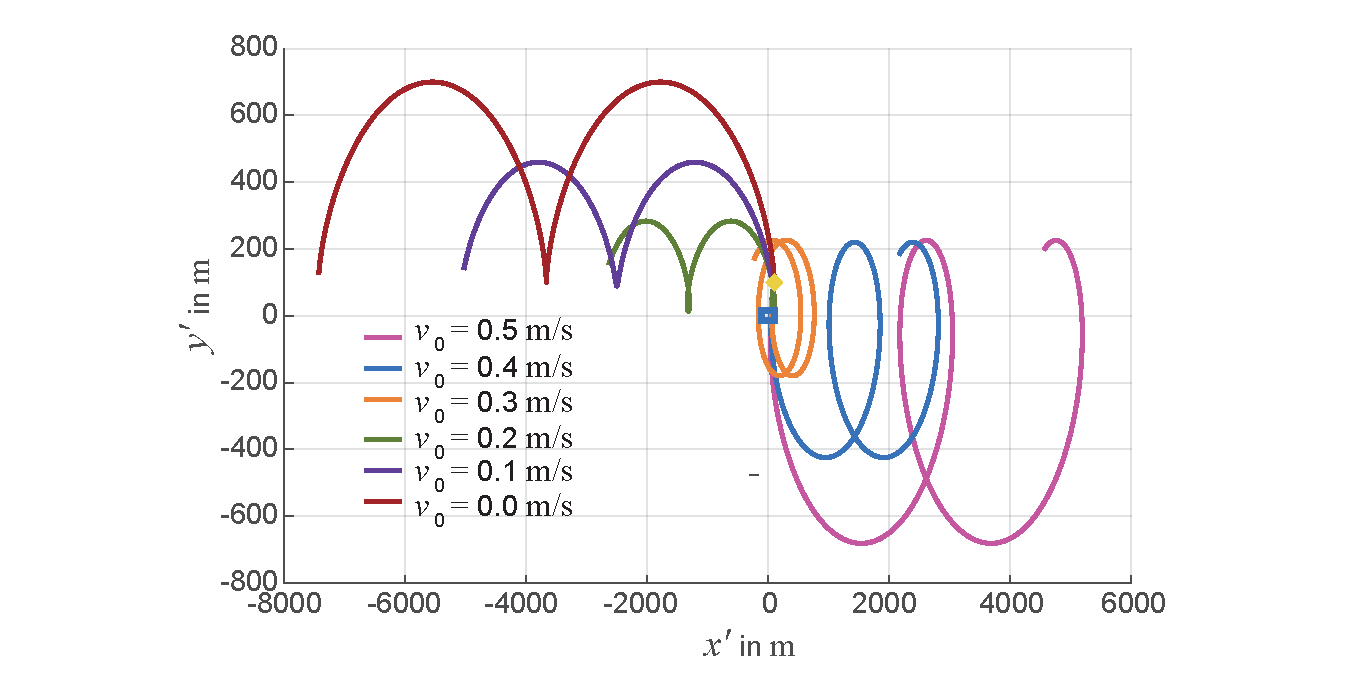
\includegraphics[width=\textwidth]{RendezvousAstronaut01.pdf} 
	%\caption[Astronaut au�erhalb der ISS.]{Astronaut au�erhalb der ISS. Der Astronaut befindet sich initial bei $x_0'=y_0'=\SI{100}{\metre}$ und bewegt sich mit einer Anfangsgeschwindigkeit $v_0$ (also keine initiale Relativgeschwindigkeit zum Ziel, d.h. $\dot{x}_0'=\dot{y}_0=0'$) genau in Richtung auf die Station zu. Selbst bei $v_0=0$ entfernt sich der Astronaut mit der Zeit von der Raumstation. Dargestellt sind die L�sungen der Clohessy-Wiltshire-Gleichungen wie im \mscr~ \mladynref{Rendezvous01.m} im Detail ausgef�hrt.}
	%\label{abb:adyn_rendezvous02}
%\end{figure}
%
  %\item[b)]
    %Was passiert, wenn der Astronaut seinen R�ckkehrantrieb (englisch \textit{Return-Thruster}) mit einem Antriebsverm�gen von $\SI{1}{\metre\per\second}$ einsetzt?   
		%Intuitiv \anf{zielt} der Astronaut mit seinem auf dem R�cksto�-Prinzip basierenden Thruster genau in Richtung ISS, also mit
    %\begin{align*}
        %\vec{v}_0 = 
        %\begin{pmatrix}
            %\dot{x}_0'\\
            %\dot{y}_0'\\
            %\dot{z}_0'
        %\end{pmatrix}
        %= \frac{1}{\sqrt{2}}
        %\begin{pmatrix}
            %1\\
            %1\\
            %0
        %\end{pmatrix}
        %\SI{}{\metre\per\second}\,.
    %\end{align*}
    %Leider wird durch die kombinierte Wirkung der Gezeiten und Coriolis-Kraft der Astronaut die ISS verfehlen, wie Gleichung \eqref{eq:adyn_rendez23} und \figref{adyn_rendezvous02} und \figref{adyn_rendezvous03}a zeigen.\\
    %\item[c)]
    %Wie muss der Astronaut beim Abfeuern seines Thrusters zielen, damit er die ISS sicher erreicht? \\
		%$\dot{x}_0'$, $\dot{y}_0'$ ergeben sich aus \eqref{eq:adyn_rendez24}. Wir k�nnen noch eine kleine Eigengeschwindigkeit des Astronauten vor dem Starten des Thrusters mit $\vec{v}_\text{vor} = \lk\dot{x}_{\text{vor},0'}, \dot{y}_{\text{vor},0'}\rk$ annehmen und erhalten den richtigen Zielwinkel:
    %\begin{align}
        %\tan\lk\gamma\rk = \frac{\Delta v_y}{\Delta v_x} = \frac{\dot{y}_0' -\dot{y}_{\text{vor},0'}}{\dot{x}_0'- \dot{x}_{\text{vor},0'}} \,. \label{eq:adyn_rendez27}
    %\end{align}
%\end{enumerate}
%In der Realit�t wird sich der Astronaut nat�rlich in kleinen Minisch�ben iterativ der ISS n�hern, doch auch daf�r gelten die abgeleiteten Formeln.
%
%\begin{figure}[H]
	%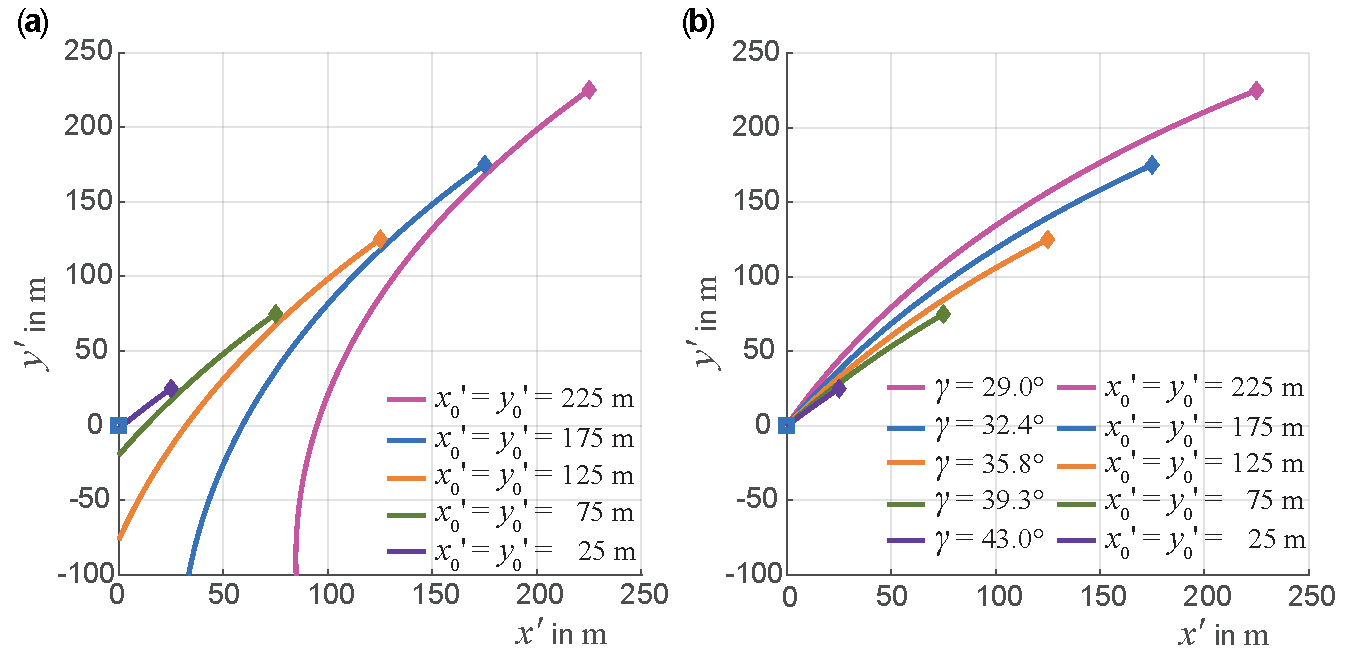
\includegraphics[width=\textwidth]{RendezvousAstronaut02.pdf} 
	%\caption[Astronaut au�erhalb der ISS.]{Astronaut au�erhalb der ISS. \fa Der Astronaut befindet sich initial bei $x_0'=y_0'=\SI{25}{\metre} \ldots \SI{225}{\metre}$ und "`zielt"' mit seinem Antriebssystem  mit einer Anfangsgeschwindigkeit $v_0$ genau in Richtung auf die Station. L�sung der Hill-Gleichungen. \fb Der Astronaut befindet sich ebenfalls initial bei $x_0'=y_0'=\SI{25}{\metre} \ldots \SI{225}{\metre}$ und bewegt sich mit einem optimierten Zielwinkel $\gamma$ der Richtung Anfangsgeschwindigkeit von $v_0 = \SI{1}{\metre\per\second}$ auf die Station zu (L�sung der Clohessy-Wiltshire-Gleichungen\index{Clohessy-Wiltshire-Gleichungen}). Offensichtlich wird der Astronaut erst bei Entfernung von kleiner als 50 m bei direkter Anzielung der Station auch bei dieser wirklich ankommen. Die Rechnungen sind im \mscr~ \mladynref{Rendezvous02.m} im Detail ausgef�hrt.}
	%\label{abb:adyn_rendezvous03}
%\end{figure}
%
%\label{bsp:adyn_stranded_astronaut}
%\end{example}
%
%

Wir verweisen auf die MATLAB-Skripte \mladynref{Rendezvous04.m} und \mladynref{Rendezvous05.m}.

\begin{figure}[H]
	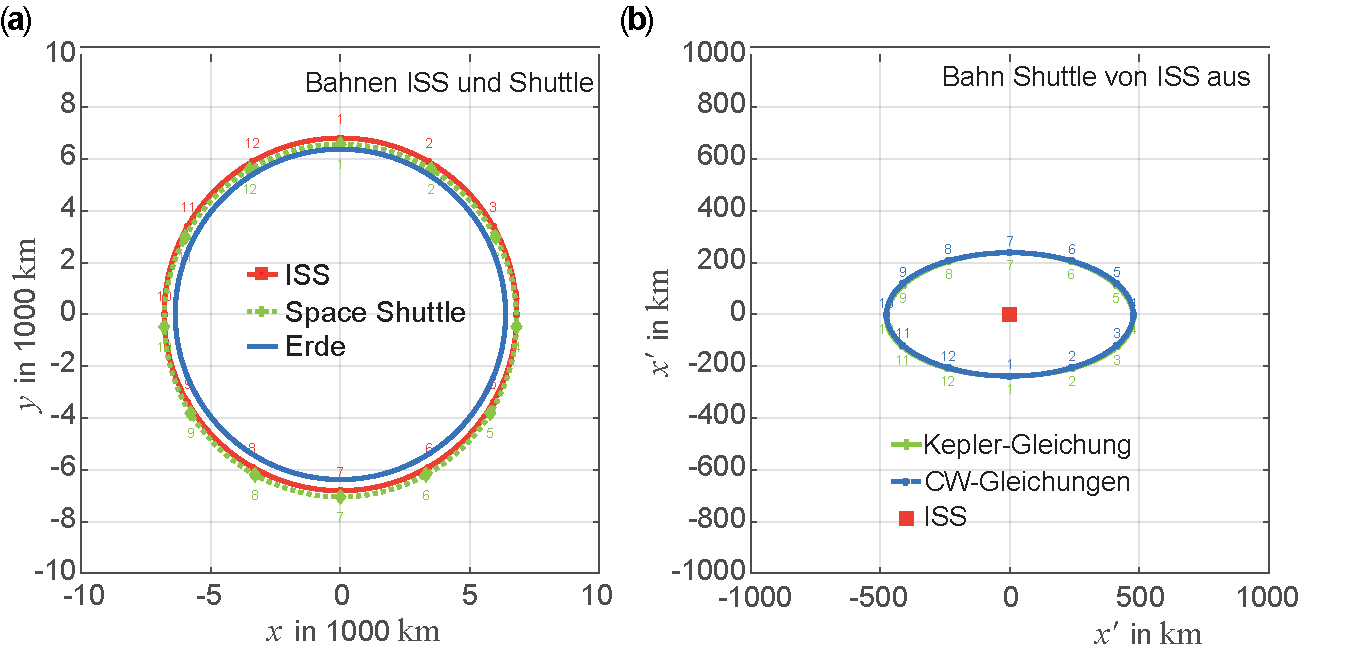
\includegraphics[width=\textwidth]{SpaceShuttle2ISS.pdf} 
	\caption[Space Shuttle und ISS in unterschiedlichen Umlaufbahnen.]{Space Shuttle und ISS in unterschiedlichen Umlaufbahnen. \fa Bahnen von ISS und Space Shuttle. Die Shuttle Bahn ist fiktiv, um das Prinzip zu erl�utern. In der Realit�t war die Shuttle Bahn viel n�her an der ISS. \fb Bahn Space Shuttle von ISS aus. L�sungen nach der Kepler-Gleichung mit Drehung des mitbewegten \KOS des Ziels und CW-L�sung im Vergleich. Die �bereinstimmung der exakten L�sungen nach der Kepler-Gleichung mit der CW-L�sung ist sehr gut, da auf Grund der Parameter die Linearisierungsbedingung f�r die CW-Gleichung relativ gut erf�llt ist.}
	\label{abb:adyn_rendezvous04Lsg}
\end{figure}

\end{sol} 
\textcolor{blue} {$\rightarrow$ zur} \probref{adyn_rendezvous01}.\\
\noindent\rule[1ex]{\textwidth}{0.5pt}  \newpage  \clearpage


%-----------------------------------------------------------------------------------------------------------

\begin{sol}{prob:adyn_rendezvous02}\label{lsg:adyn_rendezvous02} %�bung23
\textbf{Rendezvous Apollo 11 CSM und LM}\\

Die L�sung zum Rendezvous von LM und CSM von Apollo 11 in der Mondumlaufbahn ist im Detail im \mscr~\mladynref{LMCSMApollo11.m} als Berechnung der Kinematik des Rendezvous �ber die Clohessy-Wiltshire-Gleichungen ausgef�hrt. Wir erhalten die \figref{adyn_rendezvous06} aus \kap{adyn_rendezvous_apollo11}.\\

\begin{figure}[H]
	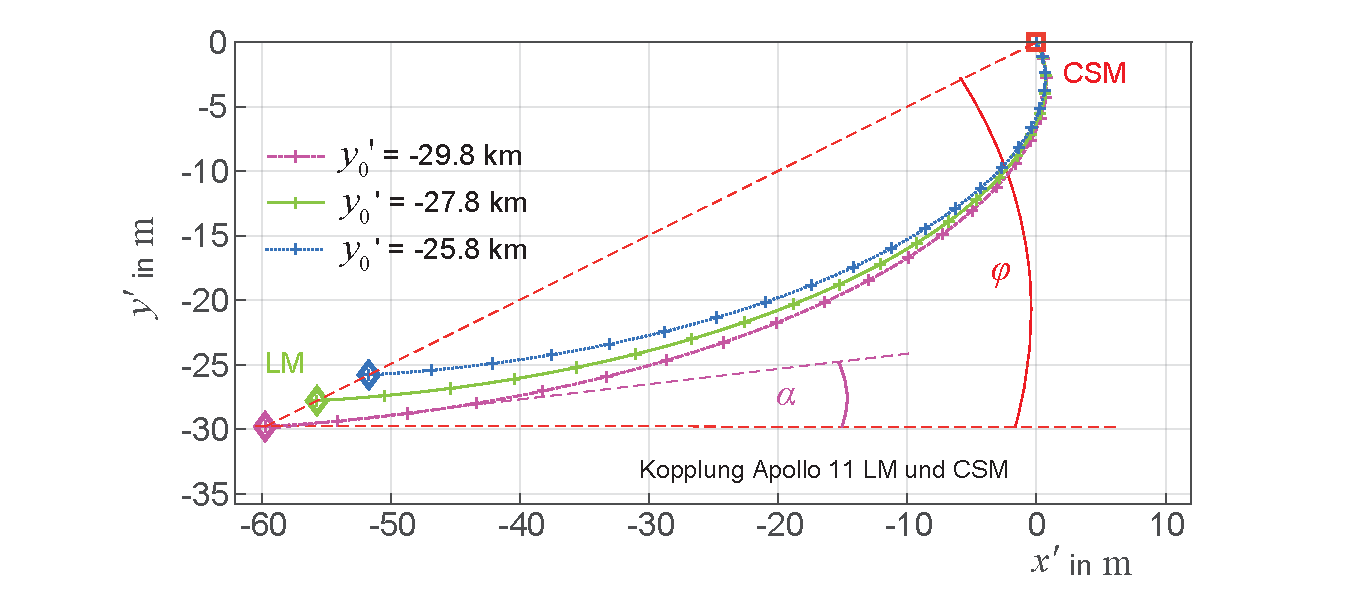
\includegraphics[width=\textwidth]{Apollo11LMCSMTrajektorie.pdf} 
	\caption[Trajektorien des LM im Anflug auf das CSM von Apollo 11.]{Trajektorien des LM im Anflug auf das CSM von Apollo 11 f�r verschiedene H�hen des TPI-Burn. Siehe \probref{adyn_rendezvous02} \bzw \mscr{}\mladynref{LMCSMApollo11.m}.}
	\label{abb:adyn_rendezvous06_uebung}
\end{figure}

\end{sol} 
\textcolor{blue} {$\rightarrow$ zur} \probref{adyn_rendezvous02}.\\
\noindent\rule[1ex]{\textwidth}{0.5pt} \newpage \clearpage 

%-----------------------------------------------------------------------------------------------------------

\begin{sol}{prob:adyn_rendezvous03}\label{lsg:adyn_rendezvous03} %�bung24
\textbf{Planung einer Apollo Mission - \textit{Free Return Trajectory}}\\

\begin{subprobs}
\subprob{Absch�tzungen}
Wir wollen als erstes eine Absch�tzung f�r die Flugzeit zum Mond treffen und nehmen dabei eine koplanare Bewegung von Flugbahn und Mondbahn an, letztere wird auch noch als Kreisbahn angenommen (\figref{adyn_FRT01}).\\
Der Punkt $\mathrm{P}_0$ (Abstand $r_0$ vom Erdzentrum) in der Parkbahn um die Erde, aus der der Einschuss (Injektion) in die translunare Bahn erfolgt, wird \textit{(Translunar Injection Point} (TLI) genannt. Dort gilt f�r die Energie und den Drehimpuls des Raumschiffs bezogen auf das Erd-\KOS:
\begin{align}
H_0 = \frac{v_0{}^2}{2} - \frac{\mu_\text{E}}{r_0}\,, & L_0 = r_0\,v_0\,\cos\gamma_0\,. \label{eq:adyn_lsg_FRT01}
\end{align}
Hierin sind $v_0\,\cos\gamma_0$ die Komponente der Raumschiff-Geschwindigkeit in Richtung lokaler Horizont mit $\gamma_0$ als der FPA bei $r_0$.\\
Damit ergeben sich f�r die Ellipse zum Mond folgende Ellipsenparameter (vergleiche auch Gleichungen \eqref{eq:hm_bewgl1} und \eqref{eq:hm_relations1}):
\begin{align}
\begin{split}
    p &= \frac{L_0{}^2}{\mu_ \text{E}}\,,~~~~ a = -\frac{\mu_\text{E}}{2H_0}\,, ~~~~
    e = \sqrt{1 - \frac{p}{a}} \,=\, \sqrt{1+\frac{L_0{}^2}{\mu_\text{E}{}^2}\,2H_0}\,~.
\end{split} \label{eq:adyn_lsg_FRT02}
\end{align}
\begin{figure}[H]
	\includegraphics[width=\textwidth]{Transfer2Moon.pdf} 
	\caption[Geometrie des Flugs zum Mond.]{Vereinfachte Geometrie des Flugs eines Raumschiffes zum Mond. Im Bild wurde eine koplanare Bewegung von Raumschiff und Mond in der Ekliptik angenommen (Draufsicht auf die Ekliptik). (Nach \cite{Bate1971}).}
	\label{abb:adyn_FRT01}
\end{figure}

In \figref{adyn_FRT01} definieren wir aus der Geometrie f�r die weitere mathematische Behandlung folgende Parameter:
\begin{align*} 
    r_0 && &\text{geozentrischer Abstand des Raumschiffs bei Injektion in die translunare Bahn} \\
    r_1 && &\text{geozentrischer Abstand des Raumschiffs beim Erreichen der SOI des Mondes}\\
    && &r_1 = \sqrt{r_{\text{EM}}{}^2 + R_{\text{SOI, M}}{}^2 - 2 r_{\text{EM}} R_{\text{SOI, M}} \cos\gamma_1} \\
    r_\text{EM} && &\text{Abstand der Massezentren von Erde und Mond}      \\
    R_\text{SOI,M} && &\text{Radius der SOI des Mondes}\\
    \varphi_0 && &\text{geozentrischer Phasenwinkel des Mondes bei Abflug (TLI) relativ zur}\\
    && &\text{Verbindungslinie Erde/Raumschiff}\\
    \varphi_1 && &\text{geozentrischer Phasenwinkel des Mondes bei Ankunft des Raumschiffs }\\
    && &\text{an der SOI relativ zur Verbindungslinie Erde/Raumschiff}\\
    \lambda_1 && &\text{selenozentrischer Winkel zwischen Ankunftsort des Raumschiffs}\\
    && &\text{an der SOI des Mondes und der Verbindungslinie Erde/Mond}\\
    \gamma_0,\gamma_1 && &\text{FPA des Raumschiffs bei TLI \bzw Ankunft an der SOI des Mondes}\\
    \upsilon_0,\upsilon_1 && &\text{wahre Anomalien der Ellipsenbahn bei TLI \bzw Ankunft SOI des Mondes}\\
    \omega_\text{M} && &\text{Umlaufgeschwindigkeit des Mondes}\,\approx \SI{2.649e-6}{\radian\per\second}\\
		a, e, P && &\text{Parameter der Transferellipse zum Mond}
\end{align*}
F�r eine Planung eines Fluges zum Mond startet man mit Vorgaben f�r $r_0,\,v_0,\,\gamma_0$ und $\lambda_1$ und berechnet die Flugzeit $t_\text{F} = \mathrm{ToF}$,\;$\varphi_0$,\, $\varphi_1$ und $\gamma_1$. Ergeben sich daraus keine sinnvollen Werte, so muss man $r_0,\,v_0,\,\gamma_0$ und $\lambda_1$ variieren. \\
Aus den Ellipsenparametern $a$, $p$, $e$ lassen sich nun bei bekannten $r_0,r_1$ die jeweiligen wahren Anomalien berechnen.
\begin{align}
\begin{split}
    \cos\upsilon_0 &= \frac{p - r_0}{\e\,r_0} \,,\\
    \cos \upsilon_1 &= \frac{p - r_1}{\e \,r_1} \quad \text{mit} \quad r_1 = \sqrt{r_{\text{EM}}{}^2 + R_{\text{SOI,M}}{}^2 - 2 r_{\text{EM}}\,R_{\text{SOI,M}} \cos \lambda_1}
\end{split}\label{eq:adyn_lsg_FRT03}
\end{align}
Die Flugzeit zum Mond ergibt sich �ber die Kepler-Gleichung zu:
\begin{align}
    t_\text{F} = t_1 - t_0 = \lk\sqrt{\frac{a^3}{\mu_\text{E}}}\rk \lek E_1 - E_0 - \e\,\lk \sin E_1 - \sin E_0\rk\rek\label{eq:adyn_lsg_FRT04}
\end{align}
wobei sich die exzentrische Anomalien $E_i~~(i=1,2)$ entweder aus
\begin{align}
\begin{split}
    \cos E_i &= \frac{\e - \cos \upsilon_i}{1 + \e \cos \upsilon_i} = \lk 1 - \frac{r_i}{a}\rk\,\frac{1}{\e}\\
    \text{oder}\quad \tan \frac{E_i}{2} &= \sqrt{\frac{1-\e}{1+\e}}\,\tan \lk \frac{\upsilon_i}{2} \rk    
\end{split}\label{eq:adyn_lsg_FRT05}
\end{align}
ergeben (\vgl Gleichungen \eqref{eq:hm_r_param_ellipse} und \eqref{eq:hm_nu(t)_alternativ}).\\
Wir brauchen noch den Winkel $\varphi_1$, dieser ergibt sich nach dem Sinussatz aus
\begin{align}
    \sin\varphi_1 = \frac{R_{\text{SOI,M}}}{r_1}\,\sin\lambda_1 \,. \label{eq:adyn_lsg_FRT06}
\end{align}
F�r eine Absch�tzung der Flugzeiten wollen wir annehmen, dass $\gamma_0 \approx 0$ ist. Wir k�nnen dann die Flugzeiten f�r verschiedene $\lambda_1$ \bzw $\varphi_1$ als Funktion der TLI-Geschwindigkeit $v_0$ berechnen.

\begin{figure}[H]
	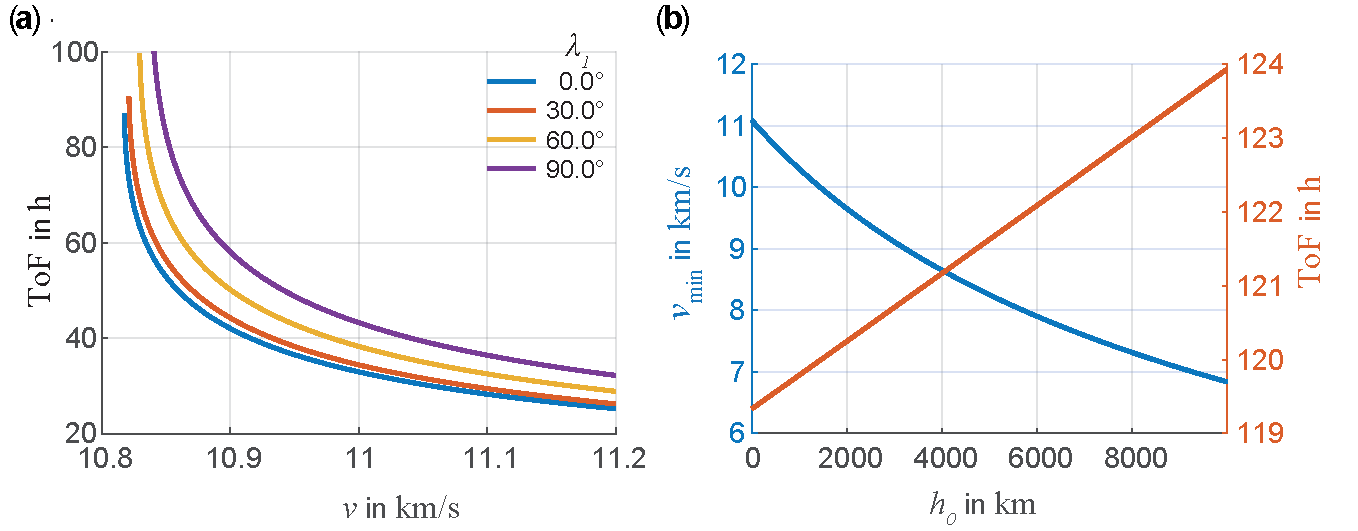
\includegraphics[width=\textwidth]{Transfer2MoonTOF.pdf} 
	\caption[Flugzeiten und Minimalgeschwindigkeit zum Mond.]{Flugzeiten und Minimalgeschwindigkeit zum Mond. \fa ToF als Funktion der TLI-Geschwindigkeit $v_0$ \fb Minimum-Geschwindigkeit $v_\text{min}$ f�r TLI und zugeh�rige ToF als Funktion des Radius $r_0$ der erdnahen Kreisbahn. Siehe \mscr~\mladynref{Transfer2Moon.m}.}
	\label{abb:adyn_FRT02}
\end{figure}

Man erkennt aus \figref{adyn_FRT02}a, dass es eine minimale Geschwindigkeit $v_{\text{min}}$ (abh�ngig vom Winkel $\lambda_1$) gibt, um �berhaupt in endlicher Zeit den Mond zu erreichen. Diese liegt bei etwas �ber $\SI{10.8}{\km\per\second}$ f�r $\lambda_1 =0$ und ist ebenfalls abh�ngig und der H�he $h_0$ der Parkbahn in Erdn�he.\\
Man kann nun eine einfache numerische Absch�tzung f�r $v_{\text{min}}$ machen, wenn man annimmt, dass die TLI am Perig�um erfolgen soll.
Dann ist definitiv $\gamma_0 = 0$ und das Apog�um der elliptischen translunaren Bahn entspricht dann $r_{\text{EM}}$ (\bzw $r_{\text{EM}} - R_{\text{SOI,M}}$, wenn wir die SOI ber�cksichtigen wollen). Wir finden also:
\begin{align}
     2a_0 &= r_0 + r_{\text{EM}} ~~~\text{und}~~~H_0 = -\frac{\mu_\text{E}}{2a} = \frac{v_{\text{min}}{}^2}{2} - \frac{\mu_\text{E}}{r_0} \nonumber \\
    \rightarrow \quad v_{\text{min}}{}^2 &= \frac{2\mu_\text{E}}{r_0}\,\lk 1 - \frac{1}{1 + r_{\text{EM}}/r_0}\rk ~~ \text{und} ~~~ \text{ToF}_{\text{max}} = \pi \sqrt{\frac{a_0{}^3}{\mu_\text{E}}} \,. \label{eq:adyn_lsg_FRT07}
\end{align}
Man erh�lt dann \zb f�r $h_0 = \SI{400}{\km}$ eine minimale notwendige Geschwindigkeit von $v_{\text{min}} = \SI{10.75}{\km\per\second}$ und eine (maximale) Flugzeit von $ \text{ToF}_{\text{max}} = \SI{119.5}{\hour}$ (\figref{adyn_FRT03}), 
was wesentlich l�nger ist, als \zb Apollo 11 zum Mond brauchte.\\
Man erkennt sehr sch�n aus \figref{adyn_FRT02}, wie kleine �nderungen der TLI-Anfangsgeschwindigkeit die Flugzeit wesentlich verk�rzen.

\subprob {\textit{Patch Conic} - N�herung}

Nach diesen grunds�tzlichen �berlegungen wollen wir nun die Bahn genauer berechnen und dabei das Konzept der SOI (siehe \kap{adyn_gravity_assist} \bzw \probref{adyn_SOI}) benutzen. Bisher haben wir ja die Gravitationswirkung des Mondes vernachl�ssigt. Wir arbeiten in den relevanten Bereichen jeweils nur mit der SOI der Erde \bzw des Mondes. Dies f�hrt auf das sogenannte Konzept der \textit{Patched Conic} (der "`aneinandergest�ckelten Kegelschnitte"', \vgl auch \probref{adyn_SOI}). 

\begin{figure}[H]
	\includegraphics[width=\textwidth]{Transfer2MoonPP.pdf} 
	\caption[Geometrie des Transfers zum Mond am \textit{Patch Point}.]{Geometrie des Transfers zum Mond am \textit{Patch Point}. Die Koordinaten im selenozentrischen \KOS werden mit dem Index 2 bezeichnet und sind in rot gezeichnet. Der Winkel $\varepsilon_2$ bezeichnet den anf�nglichen selenozentrischen Winkel der Geschwindigkeit des Raumschiffs relativ zum Mondzentrum. (Nach \cite{Bate1971}.)}
	\label{abb:adyn_FRT03}
\end{figure}

Wir berechnen zun�chst die Transferphase vom TLI bis zum Erreichen der SOI des Mondes. Dazu berechnen wir �ber \eqref{eq:adyn_lsg_FRT03}-\eqref{eq:adyn_lsg_FRT05} die ToF und auch den geozentrischen Phasenwinkel $\varphi_0$, den der Mond bei der TLI haben muss:
\begin{align}
    \varphi_0 = \upsilon_1 - \upsilon_0 - \gamma_1 - \omega_{\text{M}}\,  \lk t_1 - t_0\rk\,. \label{eq:adyn_lsg_FRT08}
\end{align}
Wir schauen uns nun genauer die Bedingungen am sogenannten \textit{Patch Point}, dem Punkt PP an. Wir bestimmen dort zun�chst die Geschwindigkeit $\vec{v}_2$ des Raumschiffs im selenozentrischen (\dh lunaren) \KOS:
\begin{align}
\begin{split}
    \vec{v}_2 &= -\vec{v}_{\text{M}} + \vec{v}_1\\
    v_2 &= \sqrt{v_1{}^2 + v_{\text{M}}{}^2 - 2 v_1\,v_{\text{M}}\,\cos \lk \gamma_1 - \varphi_1\rk} 
\end{split}\label{eq:adyn_lsg_FRT09}
\end{align}
mit
\begin{align*}
    v_{\text{M}} = \omega_{\text{M}}\,r_{\text{EM}} \approx \SI{1.018}{\km\per\second}.
\end{align*}
Ferner gilt am Punkt PP $r_2 = R_{\text{SOI,M}}$ und 
\begin{align}
    \varepsilon_2 = \arcsin \lk\frac{v_\text{M}}{v_2}\,\cos\lambda_1 - \frac{v_1}{v_2}\,\cos\lk \lambda_1 + \varphi_1-\gamma_1\rk\rk \,. \label{eq:adyn_lsg_FRT10}
\end{align}
Letztere Beziehung kann man sich ebenfalls aus \figref{adyn_FRT03} �ber
\begin{align*}
    v_2\,\sin\epsilon_2 = v_{\text{M}}\,\cos \lambda_1 - v_1\,\cos\lk\lambda_1 + \varphi_1 - \gamma_1\rk
\end{align*}
herleiten. F�r eine direkte Landung auf dem Mond muss der Winkel $\varepsilon_2$ logischerweise $0$ sein. 
F�r alle anderen F�lle kann man nun mit den \anf{lunaren} Anfangsbedingungen $r_2$, $v_2$ und $\epsilon_2$ drei m�gliche Trajektorien um den Mond herum unterscheiden:
\begin{enumerate}
    \item [1)] Aufschlag auf den Mond: In diesem Fall ist das Periselenium $r_{\text{P,M}}$ (kleinster Abstand der Bahn vom Mondzentrum) kleiner als der Mondradius $R_{\text{M}}$.
    \item [2)] Mondumlaufbahn, \dh Einschwenken auf eine Mondumlaufbahn durch Abbremsen/Beschleunigen auf die notwendige Umlaufgeschwindigkeit  $v_3$.
    \item [3)] Mondumrundung (\zb als \textit{Free Return Trajektory} (FRT)), wobei besonders das Periselenium und die Bedingungen ($r_3$, $v_3$, $\gamma_3$, $\lambda_3$) beim Verlassen der SOI des Mondes interessant sind, da diese in ma�gebliche die R�ckkehrbahn zur Erde bestimmen.
\end{enumerate}
Wir m�ssen daher als n�chstes das Periselenium $r_\text{P,M}$ berechnen, da wir das ja in jedem der drei F�lle zur Bewertung der Bahn um den Mond brauchen. In der SOI des Mondes gilt im \KOS des Mondes gilt nat�rlich wieder Energie- und Drehimpulserhaltung:
\begin{align}
\begin{split}
    H_2 &= \frac{v_2{}^2}{2} - \frac{\mu_\text{M}}{r_2}\,~~\text{mit}~~ \mu_ \text{M} = G\,M_\text{M} \,\\
		L_2 &=  r_2 \, v_2\,\cos \gamma_2 = r_2\,v_2\,\sin \varepsilon_2 \,, ~~\text{da}~~ \gamma_2 = 90^\degree - \varepsilon_2\,.
\end{split}\label{eq:adyn_lsg_FRT11}
\end{align}
Wie bei der Berechnung der Transferellipse finden wir die Kegelschnittparameter\footnote{Der Kegelschnitt wird \ia eine Hyperbel sein.} f�r die Mondbahn:
\begin{align}
    p_2 = \frac{L^2}{\mu_\text{M}}\,, \quad e_2 = \sqrt{1 + \frac{2 H_2\,L^2}{\mu_\text{M}{}^2}} \label{eq:adyn_lsg_FRT12}
\end{align}
und daraus
\begin{align}
    r_\text{P,M} = \frac{p_2}{1 + \e}\,, \quad v_\text{P,M} = \sqrt{2 \lk H_2 + \frac{\mu_\text{M}}{r_\text{P,M}} \rk} \label{eq:adyn_lsg_FRT13}
\end{align}
Wir wollen als Beispiel durchrechnen:
\begin{align*}
    r_0 &= \SI{300}{\km} + R_\text{E} = \SI{6678}{\km}\,,~~
    v_0 = \SI{10.87}{\km\per\second}\,,~~
    \gamma_0 = 0^\degree\,,~~
    \lambda_1 = 30^\degree\,.
\end{align*}
Ohne weitere Kurskorrekturen wird die geringste Entfernung zur Mondoberfl�che
\begin{align*}
    h_\text{P,M} = r_\text{P,M} - R_\text{M} = r_\text{P,M} - \SI{1737.4}{\km} = \SI{1413.6}{\km}\,.
\end{align*}
Wie bereits erw�hnt, kommt es f�r  $h_\text{P,M} < 0$ zur Landung \bzw zum Aufschlag auf dem Mond, abh�ngig von $v\lk h_\text{M} = 0\rk$ und je nach Verf�gbarkeit von Bremsm�glichkeiten.\\

\begin{figure}[H]
	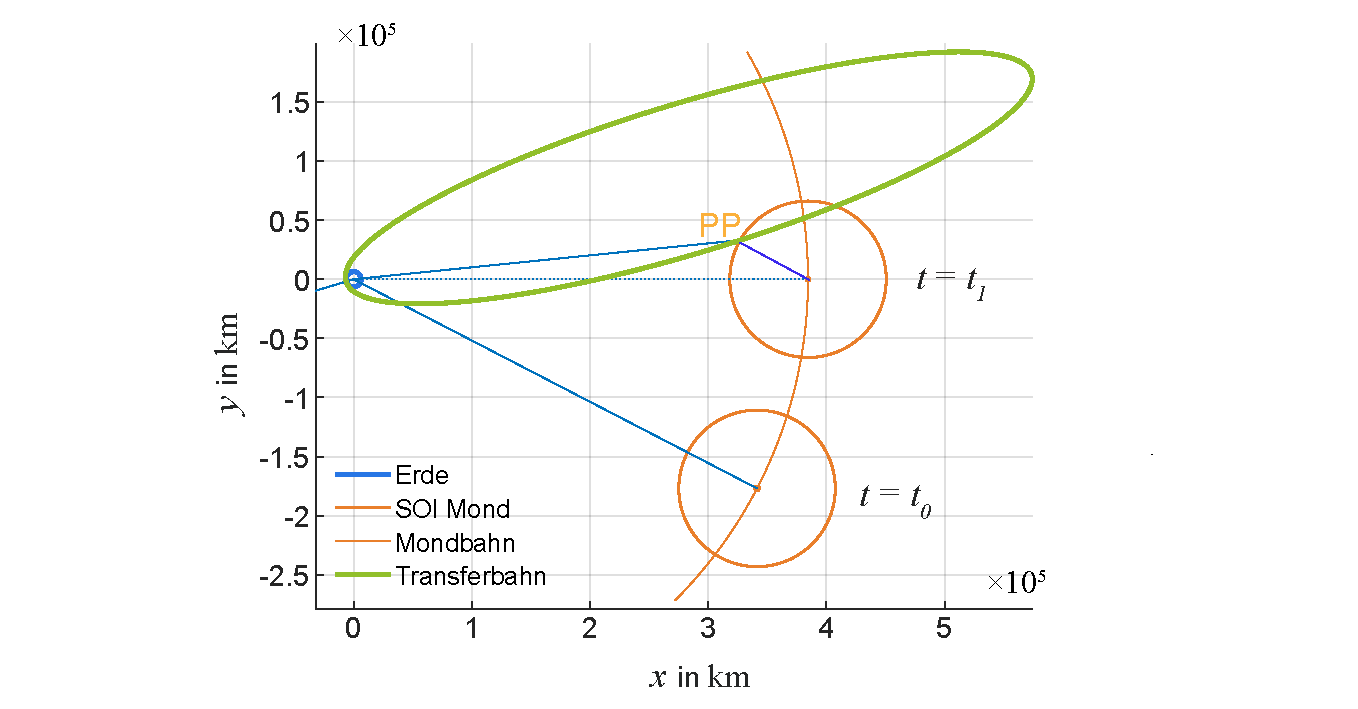
\includegraphics[width=\textwidth]{Transfer2Moon04.pdf} 
	\caption[Berechnete Geometrie des Transfers zum Mond.]{Berechnete Geometrie des Transfers eines Raumschiffes zum Mond. In der Rechnung wurde eine koplanare Bewegung von Raumschiff und Mond in der Ekliptik angenommen. Parameter siehe Tabelle \ref{tab:adyn_FRT01} und \mscr~\mladynref{Transfer2MoonExample.m}.}
	\label{abb:adyn_FRT04}
\end{figure}


Die Parameter f�r die \figref{adyn_FRT04} und \figref{adyn_FRT05} sind in folgender Tabelle gelistet:
\begin{table}[h!]
\centering
\begin{tabular}{|c|c|c|c|c|c|}
\hline
\multicolumn{6}{|l|}{\textbf{Vorgaben und Abflugparameter @TLI}} \\
\hline
$h_0$ (km) & $\gamma_0$ ($\degree$) & $v_0$ (km/s) & $\lambda_1$ ($\degree$) & &   \\
\hline
300.0 & 0.0 & 10.87 & 30.0 & &  \\
\hline
\multicolumn{6}{|l|}{\textbf{Abflugparameter @TLI}} \\
\hline
$a_0$ (km) & $p_0$ (km) & $\e_0$  & $\phi_0$ ($\degree$) &  &  \\
\hline
$\SI{3.03e5}{}$& $\SI{1.32e4}{}$& 0.9780 & 135.77 & &   \\
\hline
\multicolumn{6}{|l|}{\textbf{Parameter auf Transfer zum Mond}} \\
\hline
$v_1$ (km/s) & $v_2$ (km/s) & $\upsilon_1$ &$\upsilon_2$ & $\mathrm{TOF}$ (h) &  \\
\hline
1.054 & 1.220 &0.0 & 5.78 & 50.15&  \\
\hline
\multicolumn{6}{|l|}{\textbf{Parameter am Mond}} \\
\hline
$r_2$ (km) & $\epsilon_2$ ($\degree$) & $p_2$ (km) &$\e_2$ & $h_\text{PM}$ (km)& $\mathrm{TOF}_\text{SOI}$ (h)  \\
\hline
$\SI{6.62e4}{}$ & 4.72 & 9014.8 & 1.8610 & 1413.6 & 28.05 \\
\hline
\end{tabular}
\caption{Parameter f�r \textit{Patch Conic} N�herung} \label{tab:adyn_FRT01}
\end{table}
Hierin ist $\mathrm{TOF}$ die Flugzeit von der TLI bis zum Erreichen der SOI des Mondes und $\mathrm{TOF}_\text{SOI}$ die Flugzeit zum Durchfliegen der SOI des Mondes. \\
Insgesamt ergibt sich f�r einen Flug bis zur R�ckseite des Mondes eine Gesamtflugzeit von
\begin{align*}
    t_\text{F} = \mathrm{TOF} + \frac{1}{2} \mathrm{TOF}_\text{SOI} = \SI{50.15}{\hour} + \SI{14.025}{\hour} \approx \SI{64.175}{\hour}\,,
\end{align*}
also etwa weniger als 3 Tage und damit auch etwas schneller als Apollo 8 unterwegs war.\\

\begin{figure}[H]
	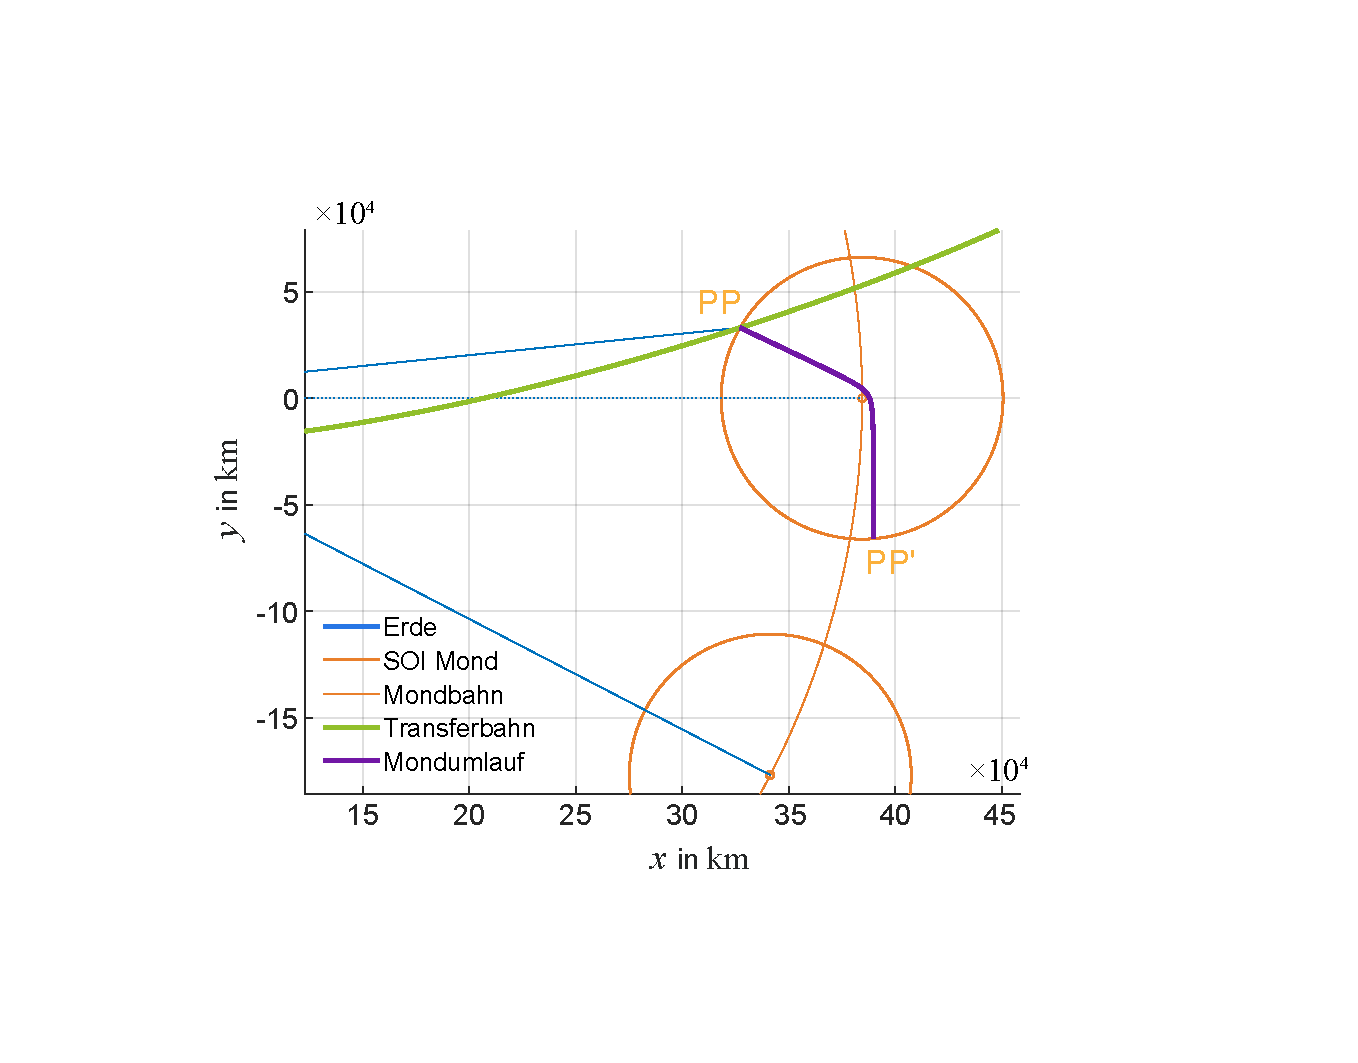
\includegraphics[width=\textwidth]{Transfer2Moon05.pdf} 
	\caption[Berechnete Geometrie des Transfers zum Mond am \textit{Patch Point}.]{Berechnete Geometrie des Transfers zum Mond am \textit{Patch Point}, sowie Mondumlauf. Die lila Kurve zeigt die Bahn des Raumschiffs im \KOS des Mondes. In der Rechnung wurde eine koplanare Bewegung von Raumschiff und Mond in der Ekliptik angenommen. Parameter siehe Tabelle Parameter siehe Tabelle \ref{tab:adyn_FRT01} und \mscr~\mladynref{Transfer2MoonExample.m}. Man beachte, dass \figref{adyn_FRT05} die Bewegung im \KOS des Mondes zeigt und nicht im als Inertialsystem angenommenen geozentrischen \KOS der Erde. F�r eine Energie $H_2 > 0$ wird $\e_2 > 1$ und damit die Bewegung um den Mond eine Hyperbel. Man �berlege sich Analogien zur Behandlung des Gravity-Assist-Man�vers in \kap{adyn_gravity_assist}.}
	\label{abb:adyn_FRT05}
\end{figure}

Man kann die Werte am Punkt PP' berechnen und dann weiter transformieren in das Erd-\KOS, um zu sehen, ob eine \textit{Free Return Trajectory} vorliegt, ganz analog wie beim Swing-By-Man�ver.\\
Wir wollen jedoch im Folgenden die Rechnungen komplett, also auch die Bewegung um den Mond herum im Inertialsystem numerisch machen und k�nnen dabei als Startwert die Parameter der \textit{Patch Conic}-Rechnung �bernehmen.

\newpage
\subprob{Numerische Rechnung Vergleich \textit{Patch Conic} und 1. N�herung}

Wir wollen nun konkret den Raumflug von Apollo 13 anschauen und w�hlen  entsprechend des NASA Flight Journal (\url{https://www.nasa.gov/history/afj/ap13fj/index.html}) $h_0=\SI{169.609}{\km}$. Ebenso benutzen die Ergebnisse der \textit{Patch Conic} N�herung (\figref{adyn_FRT06}) als Startwerte f�r die numerische Rechnung und betrachten zun�chst die Erde als ruhend und den Mond auf einer Kreisbahn umlaufend. 

\begin{figure}[H]
	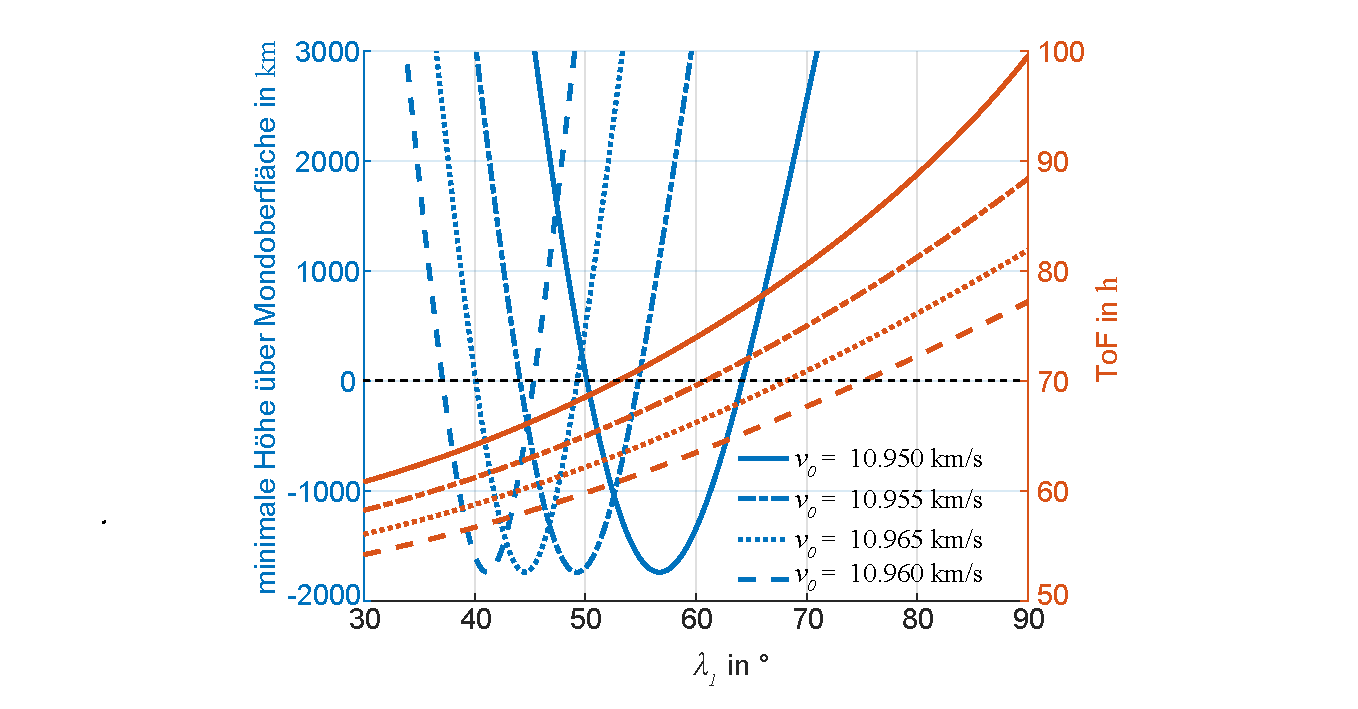
\includegraphics[width=\textwidth]{PatchConicApollo13.pdf} 
	\caption[Ergebnisse der \textit{Patch Conic} N�herung f�r Apollo 13.]{Ergebnisse der \textit{Patch Conic} N�herung f�r Apollo 13.}
	\label{abb:adyn_FRT06}
\end{figure}

Wir erhalten dann \zb f�r $v_0 = \SI{10960.0}{\km\per\second}$ in der
\textit{Patch Conic} N�herung:\\
\begin{align*}
	\lambda_1      &: 49.70\degree  && \\ 
	\varphi_0      &: 129.89\degree\\ 
	\mathrm{ToF} &: 78.7\,\mathrm{h}\\ 
	h_\text{P,M} &: \SI{279.3}{\km} \, 
\end{align*}
was schon relativ gut mit den tats�chlichen Werten von Apollo 13 �bereinstimmt, wobei man ber�cksichtigen muss, dass beim tats�chlichen Raumflug es eine Reihe von Kurskorrekturen gab.

In der numerische Betrachtung (L�sung der Bewegungsgleichungen) ergeben sich dann eine Vielzahl von L�sungen. Das liegt daran, dass es sich bei der Bestimmung der FRT ja um ein Optimierungsproblem handelt, bei dem $h_0$, $h_\text{Reentry}$ und $h_\text{P,M}$ gegeben sind und $v_0$ und $\varphi_0$ gesucht werden. F�r solche Optimierungsprobleme gibt es h�ufig keine eindeutigen L�sungen. Wir erhalten \zb f�r $v_0 = \SI{10960.0}{\km\per\second}$ und $\varphi_0 = 129.33\degree$:
\begin{align*}
	\mathrm{ToF}\, \text{zum Mond} &: 78.2\,\mathrm{h}\\ 
	\mathrm{ToF}\, \text{Gesamt} &: 156.4\,\mathrm{h}\\ 
	h_\text{M,P}\, \text{Mond} &: \SI{2111.0}{\km}\\
	h_\text{Reentry}\, \text{Erde} &: \SI{150.0}{\km} 
\end{align*}
Die L�sung ist im Detail im \mscr~\mladynref{FreeReturnTrajectoryApollo13.m} ausgef�hrt.\\

\subprob{Genauere Rechnungen f�r Apollo 13}

Bisher haben wir die Erde als ruhend angenommen und den Mond auf einer Kreisbahn um diese rotierend, Wir betrachten nun das vollst�ndige Dreik�rper-Problem Erde, Mond und Apollo 13 im Schwerpunktsystem von Erde-Mond. Wiederum handelt sich hierbei um ein Optimierungsproblem, bei dem $h_0$ und $h_\text{Reentry}$ gegeben sein sollen und $v_0$, $\varphi_0$ und $h_\text{P,M}$ gesucht werden.
Die Rechnungen ergeben in diesem Fall beispielhaft, 
\begin{align*}
	v_0      &: \SI{10963.0}{\km\per\second}\\ 
	\varphi_0      &: 130.46\degree\\ 
	\mathrm{ToF}\, \text{zum Mond} &: 75.2\,\mathrm{h}\\ 
	\mathrm{ToF}\, \text{Gesamt} &: 149.5\,\mathrm{h}\\ 
	h_\text{P,M}\, \text{Mond} &: \SI{1353.4}{\km}\\
	h_\text{Reentry}\, \text{Erde} &: \SI{169.6}{\km} \,,
\end{align*}
wobei wir hier vor darauf geachtet haben, dass der Wiedereintritt in die Erdatmosph�re gew�hrleistet ist, daf�r der Mondabstand etwas gr��er gew�hlt ist.
Das L�sungsbeispiel ist in \figref{adyn_FRT08} dargestellt und im Detail im \mscr~\mladynref{FreeReturnTrajectoryApollo13CoM.m} ausgef�hrt.\\

\begin{figure}[H]
	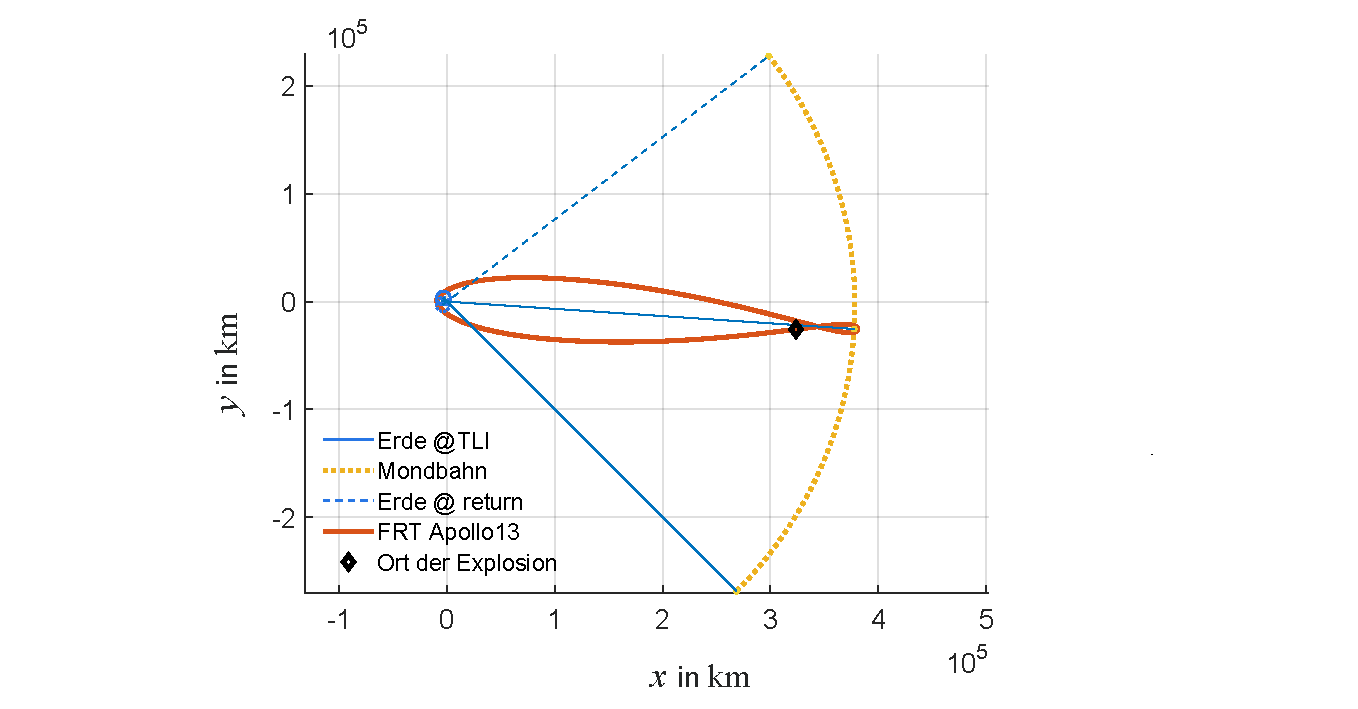
\includegraphics[width=\textwidth]{FRTApollo13.pdf} 
	\caption[Ergebnisse der numerischen Rechnung f�r eine \textit{Free Return Trajectory } f�r Apollo 13.]{Ergebnisse der numerischen Rechnung f�r eine \textit{Free Return Trajectory} im Schwerpunktsystem Erde-Mond. In der Graphik ist auch der Ort der Explosion des Tanksystems von Apollo 13 eingezeichnet.}
	\label{abb:adyn_FRT08}
\end{figure}

\newpage	
\subprob{Allgemeine Bemerkungen - Alternative Ans�tze}

Wie bereits erw�hnt, handelt es sich bei der Bestimmung der FRT um ein Optimierungsproblem. \cite{Battin1999, Brown2002, Bate1971, Vallado2007}. 
Bei der L�sung desselben findet man, dass die L�sungswerte $h_\text{P,M},\, h_\text{Reentry}$ sehr stark auf kleinere Ver�nderungen der Eingabeparameter variieren, \zb wird bei kleinsten �nderungen der Anfangsgeschwindigkeit (TLI-Geschwindigkeit) $v_0$ oder des TLI-Phasenwinkels $\varphi_0$ bei ansonsten festgehaltenen Parametern die Reentry-Flugbahn sehr stark variieren, was bedeuten k�nnte, dass das Raumschiff auf der FRT entweder in der Erdatmosph�re vergl�ht oder von dieser abprallt (siehe \kap{adyn_reentry}).\\
In der Realit�t wird man deswegen die Missionsplanung im Verlauf einer FRT mit kleineren Kurskorrekturen versehen, die wesentliche gr��ere Toleranzen der Parameter ($v_0$, $\varphi_0$) erlauben. Man kann in diesem Fall auch als weitere Randbedingung f�r die Optimierungsaufgabe einen minimalen Treibstoffverbrauch f�r die Summe der einzelnen Kurskorrekturen und Bahn�nderungen fordern, also f�r
\begin{align*}
    \Delta v_{\text{ges}} = \Delta v_{\text{TLI}} + \Delta_\text{Cor,E$\to$M} + \Delta v_{\text{LOI}} + \Delta v_{\text{TEI}} + \Delta_\text{Cor,M$\to$E} + \Delta v_{\text{EOI}}
\end{align*}
Hierbei bedeuten:
\begin{align*}
    \Delta_\text{Cor,E$\to$M} &: \text{Geschwindigkeitsbudget f�r Kurskorrektur auf dem We g $E \to M$ (\bzw $M \to E$)}\\
    \Delta v_\text{LOI,EOI} &: \text{Geschwindigkeitsbudget f�r Lunar Orbit Injektion \bzw Earth Orbit Injektion}\\
    \Delta v_{\text{TEI}} &: \text{Geschwindigkeitsbudget f�r Trans Earth Injektion}
\end{align*}
Dem interessierten Leser sei auf die Ref. \cite{Gagg2016} verwiesen, in welcher auch die einzelnen Schritte der mathematischen Optimierung\footnote{Die Optimierungsprobleme sind generell interessante mathematische Probleme, deren allgemeine Behandlung �ber den Umfang dieses Buches hinaus geht. Wir sind bereits bei der Herleitung der Lagrange-Gleichungen in Band I auf ein Problem dieser Art gesto�en und beim Lambert-Problem.} erl�utert sind.\\
Ebenso verweisen wir auf die unter \url{https://de.mathworks.com/matlabcentral/fileexchange} aufgef�hrten Programme  mit verschiedenen Optimierungsprozeduren in zum Teil vereinfachten Geometrien f�r die Berechnung der FRT.\footnote{ Wir verweisen insbesondere auf:\\
\url{Lunar Free-Return Trajectory Analysis with MATLAB - OTB - File Exchange - MATLAB Central (mathworks.com)},\\ \url{Lunar Free-Return Trajectory Analysis with MATLAB - File Exchange - MATLAB Central (mathworks.com)} und \\
\url{N-body Lunar Free Return Trajectory Analysis � OTB - File Exchange - MATLAB Central (mathworks.com)}.} \\

Wir wollen jedoch noch einen anderen Bezug herstellen. In Kap. 1.2.3.6 in Band I hatten wir das Drei-K�rper-Problem und insbesondere auch das sogenannte eingeschr�nkte Drei-K�rper-Problem eingef�hrt, bei welchem eine dritte Testmasse deutlich kleiner ist als die beiden anderen Massen. Bei dem FRT-Problem handelt es sich genau um ein solches Problem, welches wir im mitrotierenden \KOS (um den Schwerpunkt des Erde-Mond-Systems) wie folgt schreiben k�nnen (\vgl Gl. (1.100) in Band I), wobei wir die Striche f�r das mitbewegte System weglassen wollen. 
\begin{subequations}
\begin{align}
    \ddot{x}_\text{R} - 2\omega_\text{M}\,\dot{y}_\text{R}- \omega_\text{M}{}^2\,x_\text{R} &= -\frac{\mu_\text{E}}{r_{\text{RE}{}^3}}\,\lk x_\text{R} + m_\text{eff,M}\,r_{\text{EM}}\rk -\frac{\mu_\text{M}}{r_{\text{RM}{}^3}}\,\lk x_\text{R} - m_\text{eff,E}\,r_{\text{EM}}\rk\\
    \ddot{y}_\text{R} + 2 \omega_\text{M}\,\dot{x}_\text{R}  - \omega_\text{M}{}^2\,y_\text{R}  &= -\frac{\mu_\text{E}}{r_{\text{RE}{}^3}}\,y_\text{R} - \frac{\mu_\text{M}}{r_{\text{RM}{}^3}}\,y_\text{R}\,\label{eq:FRT_20}
\end{align}  
\end{subequations}
mit 
\begin{align*}
    r_\text{RE} = \left| \vec{r}_\text{R} - \vec{r}_\text{E} \right|, \quad
    r_\text{RM} = \left| \vec{r}_\text{R} - \vec{r}_\text{M} \right|, \quad
		m_\text{eff,E} = \frac{M_{\text{E}}}{M_{\text{E}} + M_{\text{M}}} \quad \text{und} \quad 
		m_\text{eff,M} = \frac{M_{\text{M}}}{M_{\text{E}} + M_{\text{M}}}\,.
\end{align*}
Setzt man die Anfangsbedingungen ($r_0, v_0$ \bzw $x_\text{R,0},y_\text{R,0},\dot{x}_\text{R,0},\dot{y}_\text{R,0}$) ein, erh�lt man als L�sung $\lk x_\text{R},y_\text{R}\rk$ die achtf�rmige Kurve nach \figref{adyn_FRT10}.

\begin{figure}[H]
	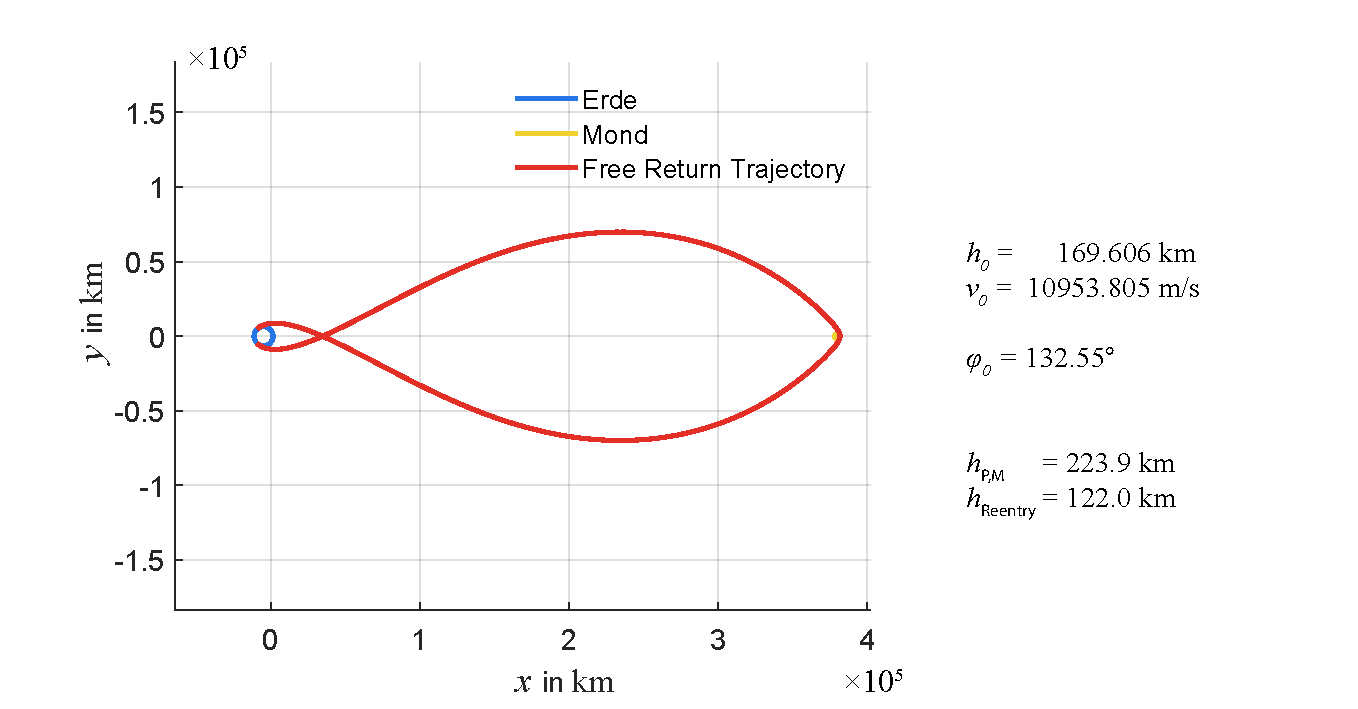
\includegraphics[width=\textwidth]{Transfer2MoonRotatingKOS.pdf} 
	\caption[Ergebnisse der numerischen Rechnung f�r das eingeschr�nkte Drei-K�rper-System Erde-Mond-Raumschiff.]{Ergebnisse der numerischen Rechnung f�r das eingeschr�nkte Drei-K�rper-System Erde-Mond-Raumschiff im mitrotierenden Koordinatensystem. Man beachte die unterschiedliche Form der Bahn, die wesentlich von der in \figref{adyn_FRT08} abweicht, was durch die unterschiedliche "`Perspektive"' des mitrotierenden Beobachters zustande kommt.}
	\label{abb:adyn_FRT10}
\end{figure}

Zum Schluss m�chten wir noch einmal bemerken, dass die FRT ein sch�nes Beispiel eines Swing-By-Man�vers (Gravity-Assist-Man�vers) (siehe \kap{adyn_gravity_assist}) beinhaltet und zwar ein Man�ver, bei welchem die Masse des Gravity-Assist-Himmelsk�rpers (in diesem Fall der Mond) abbremsend wirkt, da die Bahn nach \figref{adyn_swingby00} vor dem Himmelsk�rper liegt.

\end{subprobs}

\end{sol} 
\textcolor{blue} {$\rightarrow$ zur} \probref{adyn_rendezvous03}.\\
\noindent\rule[1ex]{\textwidth}{0.5pt}  \newpage  \clearpage

%-----------------------------------------------------------------------------------------------------------

\subsection{�bungen zu Starts aus der Erdatmosph�re und Wiedereintritt}

\noindent\rule[1ex]{\textwidth}{0.5pt} 

%-----------------------------------------------------------------------------------------------------------

\begin{sol}{prob:adyn_launch01a}\label{lsg:adyn_launch01a} %�bung25
\textbf{Bewegungsgleichungen f�r Raketenstart von Erdoberfl�che}\\

\begin{nebenrechnungNeu} {Nat�rliche Koordinaten}

(siehe \cite{Arens2008, Riley2006, Otto2019 })\\

Der zeitabh�ngige Einheitsvektor $\vec{t}$ der Tangente an die Bahnkurve (Tangentialvektor) ist definiert durch:
\begin{align}
    \vec{t} = \frac{\D \vec{r}}{\D s} ~~~\text{mit}~~~~\D s = | \D \vec{r}(t) | = \left| {\frac{\D \vec{r}}{\D t}} \right| \,  \D\,t= v(t)\; \D\,t\,,
\label{eq:adyn_NR_launch01}
\end{align}
worin $\D s$ die differentielle Bahnl�nge ist und $v$ der Betrag der Geschwindigkeit $\vec{v}$. Der Hauptnormalenvektor (ebenfalls eine Einheitsvektor) ist die 
normierte �nderung des Tangentialvektors �ber die Bahnl�nge:
\begin{align}
    \vec{n} = \frac{\D \vec{t}}{\D s} \big/ \left|\frac{\D \vec{t}}{\D s} \right|\,.
\label{eq:adyn_NR_launch02}
\end{align}
Aus $\vec{t}^2 =1 $ folgt $\D \vec{t} / \D s \cdot \vec{t} = 0$, \dh $\vec{n} \bot \vec{t}$, also $\vec{n} \cdot \vec{t} = 0$.
Damit kann man einen dritten Vektor definieren, der senkrecht auf dem Tangential- und dem Hauptnormalenvektor steht und Binormalvektor hei�t:
\begin{align}
    \vec{h} =  \vec{t} \times \vec{n}\,.
\label{eq:adyn_NR_launch03}
\end{align}
Die drei Vektoren $\vec{t},\,\vec{n},\, \vec{h}$ bilden ein (sogenanntes nat�rliches) Koordinatendreibein, das sich mit dem bewegten Objekt auf der Bahn mitbewegt und dabei sowohl einer Translation als auch Rotation unterliegt.
Die Geschwindigkeit $\vec{v}$ und die Beschleunigung $\vec{a}$ sind in diesen Koordianten dann definiert durch (\vgl Kap. 1.2.2. in Band I) 
\begin{align}
    \begin{split}
		    \vec{r} &=  v\,\vec{t}\\
        \vec{a} &=  \frac{\D}{\D t}\,\lk v\,\vec{t}\rk = \,\lek \dot{v}\,\vec{t} + v\,\dot{\vec{t}}\rek = \lek \dot{v}\,\vec{t} + v\,\vec{\omega}\times \vec{v}\rek\,.
    \end{split} \label{eq:adyn_NR_atmos03}
\end{align}
Hierin ist $\vec{\omega}$ die momentane Rotationsfrequenz des mitrotierenden \KOS definiert durch $\vec{t},\, \vec{n}$ und \vec{h}.\\

\end{nebenrechnungNeu}

Wir wollen zun�chst die momentane Rotationsfrequenz des nat�rlichen Dreibeins als Funktion von Bahnradius $r$ , Geschwindigkeit $v$ und FPA $\gamma$ berechnen. Wir betrachten dazu \figref{adyn_ueb_atmos01} und finden:
\begin{align}
    \vec{\omega} = \vec{\omega_1} + \vec{\omega_2} = (\omega_1 + \omega_2)\,\vec{h}\,,\label{eq:adyn_ueb_atmos05}
\end{align}
worin $\omega_1\,\vec{h}$ die Drehung durch die reine Bahnbewegung beschreibt und $\omega_2\,\vec{h}$ die Drehung des FPA ber�cksichtigt. Der Betrag von $\vec{\omega_1}$ ergibt sich aus \figref{adyn_ueb_atmos01} �ber $r\,\D\upsilon = |\D \vec{r}|\,\cos\gamma$ zu
\begin{align}
        \omega_1 = \dot{\upsilon} &= \frac{|\vec{v}|}{r}\,\cos\gamma = \frac{v}{r}\,\cos\gamma\, \label{eq:adyn_ueb_atmos05a} \,,
\end{align}
w�hrend der Betrag von $\vec{\omega_2}$ einfach der �nderungsrate des FPA entspricht (man beachte die Richtung!):
\begin{align}
        \omega_2 = - \dot{\gamma} \,.\label{eq:adyn_ueb_atmos05b}
\end{align}
Um die Bewegungsgleichung \eqref{eq:adyn_launch_vec},
\begin{align}
    m_\text{R}\lk t\rk \,\ddot{\vec{r}} = \vec{F}_\text{S}\lk t\rk + m_\text{R}\lk t\rk\,\vec{g}\lk \vec{r}\rk + \vec{F}_\text{D}\lk \vec{r},\dot{\vec{r}}\rk + \vec{F}_\text{A}\lk \vec{r},\dot{\vec{r}}\rk\, , \label{eq:adyn_ueb_atmos01}
\end{align}
in nat�rlichen Koordinaten schreiben zu k�nnen, schreiben wir die Kr�fte \bzw Beschleunigungen in \eqref{eq:adyn_ueb_atmos01} unter Ber�cksichtigung der Geometrie von \figref{adyn_launch02} in nat�rlichen Koordinaten (die Bewegung und alle Kr�fte sollen in einer Ebene liegen) und benutzen dabei den Angle of Attack $\alpha$ und den Flight Path Angle $\gamma$:
\begin{align}
\begin{split}
				\vec{F}_\text{S} &= F_\text{S}\,\cos\alpha\,\vec{t} + F_\text{S}\,\sin\alpha\,\vec{n}\,,~~~~\vec{F}_\text{A}  = F_\text{A}\,\vec{n}\,,~~~
        \vec{F}_\text{D} = -F_\text{D}\,\vec{t}\,,~~~\vec{g} = -g\,\sin\gamma\,\vec{t} -g\,\cos\gamma\,\vec{n}\,.
\end{split}\label{eq:adyn_ueb_atmos02}
\end{align} 
\begin{figure}[H]
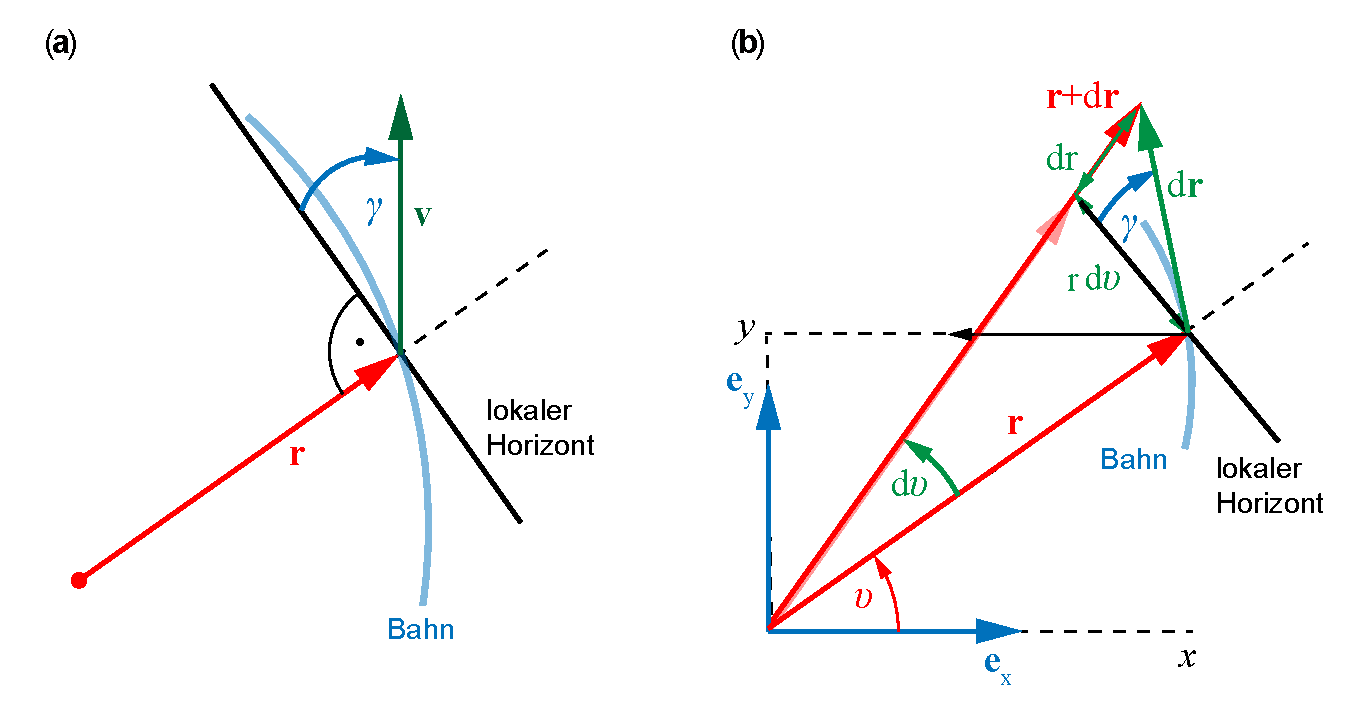
\includegraphics[width=\textwidth]{KOSReentry.pdf}
\caption[Zur Berechnung der Komponenten des Radialvektors einer Bahn im Inertialsystem der Erde.]{Zur Berechnung der Komponenten des Radialvektors einer Bahn im im Inertialsystem der Erde und im zylindrischen \KOS $\vec{t},\, \vec{n},\,\vec{h}$. \fa Lokaler Horizont, Geschwindigkeit und Flight Path Angle (FPA) $\gamma$. \fb Infinitesimale �nderungen von $r, \,\gamma$  und $v$. Der Winkel $\upsilon$ ist der Orbitalwinkel der Bahn (entspricht in etwa der wahren Anomalie) zwischen dem geozentrischen Ortsvektor zum Startpunkt und dem Ortsvektor zum Raumschiff zur Zeit $t$.}  

\label{abb:adyn_ueb_atmos01}
\end{figure}
Wir setzen \eqref{eq:adyn_ueb_atmos02} in \eqref{eq:adyn_ueb_atmos01} ein und erhalten eine Gleichung f�r $\vec{t}$ und $\vec{u}$.
\begin{align}
    \begin{split}
        \ddot{\vec{r}} &= \frac{\D}{\D t}\,\lk v\,\vec{t}\rk =  \lek \dot{v}\,\vec{t} + v\,\dot{\vec{t}}\rek = \lek \dot{v}\,\vec{t} + v \, \vec{\omega}\times \vec{v}\rek \\
        &= \lek \frac{F_\text{S}\,\cos\alpha - F_\text{D}} {m_\text{R}} \,- \,g\,\sin\gamma \rek\,\vec{t} + \lek \frac{F_\text{S}\,\sin\alpha + F_\text{A}}{m_\text{R}} - \,g\,\gamma\,\cos\gamma \rek\,\vec{n}\,.
    \end{split} \label{eq:adyn_ueb_atmos03}
\end{align}

Mit \eqref{eq:adyn_ueb_atmos05} - \eqref{eq:adyn_ueb_atmos05b} in \eqref{eq:adyn_ueb_atmos03} erhalten wir daraus jeweils eine Gleichung f�r $\vec{t}$ und 
$\vec{n}$, die jede f�r sich erf�llt sein muss, woraus folgt:
\begin{subequations}
    \begin{align}
        \dot{v}\,\vec{t} &= \lek \frac{F_\text{S}\,\cos\alpha-F_\text{D}}{m_\text{R}} - g\,\sin\gamma \rek\,\vec{t} \,, \\
        v\,\vec{\omega}\times \vec{v} &= \lk \dot{\theta}-\dot{\gamma}\rk\,\vec{h} \times v\,\vec{t}  = - \lek \frac{v^2}{r}\,\cos\gamma - v\, \dot{\gamma} \rek\,\vec{n} = \lek \frac{F_\text{S}\,\sin\alpha + F_\text{A}}{m_\text{R}} - \gamma\,g\,\cos\alpha \rek \,\vec{n}\,.
    \end{align} \label{eq:adyn_ueb_atmos04}
\end{subequations}

Nach einfacher Umformung erhalten wir schlie�lich die zwei verkoppelten skalaren Differentialgleichungen f�r $v$ und $\gamma$:
\begin{subequations}
    \begin{align}
        \dot{v} &= \frac{F_\text{S}\,\cos\alpha - F_\text{D}}{m_\text{R}} - g\,\sin\gamma\,,\\
        \dot{\gamma} &= \frac{F_\text{S}\,\sin\alpha + F_\text{A}}{v\,m_\text{R}} - \lk \frac{g}{v} -\frac{v}{r}\rk\,\cos\gamma\,~.
    \end{align}\label{eq:adyn_ueb_atmos06}
\end{subequations}

F�r den projizierten Kreisbogen $s(t)$, den das Raumschiff (eigentlich der Koordinatenursprung des mitbewegten \KOS) auf der Erdoberfl�che s(t) beschreibt, den Abstand des Raumschiffs vom Erdmittelpunkt  $r$ \bzw seine H�he $h$ �ber der Erdoberfl�che finden wir leicht aus geometrischen �berlegungen (\figref{adyn_launch02} und \figref{adyn_ueb_atmos01}):

\begin{subequations}
    \begin{align}
        \dot{h} &= v\,\sin\gamma\,,\\ 
        \dot{s} &= \frac{R_\text{E}}{r}\,v\,\cos\gamma \,=\, \frac{1}{1+h/R_\text{E}}\,v\,\cos\gamma  \,.
    \end{align}\label{eq:adyn_ueb_atmos07}
\end{subequations}

Das Differential-Gleichungssystem \eqref{eq:adyn_ueb_atmos06} und \eqref{eq:adyn_ueb_atmos07} bestimmt damit vollst�ndig die Aufstiegsbahn im mitbewegten KOS. Diese Bahn liegt in der durch die Richtungen von $s$ und $h = r - R_\text{E}$ bestimmten Ebene. 

\end{sol} 
\textcolor{blue} {$\rightarrow$ zur} \probref{adyn_launch01a}.\\
\noindent\rule[1ex]{\textwidth}{0.5pt}  \newpage  \clearpage
%-----------------------------------------------------------------------------------------------------------

\begin{sol}{prob:adyn_launch01}\label{lsg:adyn_launch01} %�bung26
\textbf{Raketenstart von verschiedenen Weltraumzentren}\\

\begin{subprobs}
\subprob{Allgemeine Betrachtungen}

\begin{figure}[H]
	\includegraphics[width=\textwidth]{Aufstiegsbahnen.pdf} 
	\caption[Transfer eines Raumschiffs von der Erdoberfl�che in einen Erdorbit �ber eine Hohmann-Ellipse.]{Transfer eines Raumschiffs von der Erdoberfl�che in einen Erdorbit �ber eine Hohmann-Ellipse. \fa idealisierter Fall ohne Reibung \fb realistischer Fall bei Vorhandensein einer Atmosph�re. Im idealisierten Fall w�rde man die Rakete horizontal direkt in die Hohmann-Ellipse starten lassen, im Fall \fb aus aerodynamischen und strukturellen senkrecht zum Horizont und f�hrt dann eine Nickkorrektur aus, um das Raumschiff einen \textit{Gravitation Turn}\index{Gravitation Turn}\index{Schwerkraftdrehung}  machen zu lassen. Siehe unten im Text.}
	\label{abb:adyn_launch_lsg_Schema}
\end{figure}

Wir k�nnen die Berechnungen vorteilhafter weise im in \kap{adyn_launch} eingef�hrten mitbewegten \KOS tun, da es uns nur um die Dynamik und nicht um eine geographische Berechnung der Bahn geht.\\
Zielstellung der Berechnung ist, das Raumschiff in eine Kreisbahn mit der H�he $h_\text{K}$ (numerische Werte beispielhaft f�r $h_\text{K}= \SI{300}{\km}$) zu bringen.\\
Ohne Atmosph�re w�rde man das Raumschiff horizontal in Richtung Osten von der Erde starten lassen (\figref{adyn_launch_lsg_Schema}a  und zwar mit einem Geschwindigkeitsbudget von
\begin{align}
	\Delta v_0 = \sqrt{\frac{G\,M_\text{E}}{R_\text{E}+h}} - \Delta v_\text{E,t} = \sqrt{\frac{G\,M_\text{E}}{R_\text{E}+h}} - \frac{2\pi\,R_\text{E}\,\cos\varphi_0}{\SI{86125}{\second}}\approx \SI{7.7309}{\km\per\second} - \SI{0.465}{\km\per\second}\,\cos\varphi_0 \,,
\end{align}
worin $\varphi_0$ die geographische Breite des Abschussortes ist und $\Delta v_\text{E,t}$ die Tangentialgeschwindigkeit auf der Erdoberfl�che der Erdrotation bezeichnet.
Das Raumschiff bewegt sich in diesem idealisierten Fall auf einer Hohmann-Ellipse (\kap{adyn_hohmann_transfer}) mit der Halbachse $a_\text{T}$ und der Exzentrizit�t $e_\text{T}$ (Numerische Werte f�r $h=\SI{300}{\km}$.)
\begin{align*}
	a_\text{T} &= \frac{1}{2} \, \lk R_\text{E} + h + R_\text{E} \rk = R_\text{E}+\frac{h}{2} \approx \SI{6528}{\km} \,,\\
  e_\text{T} &= \frac{h}{2R_\text{E}+h } \approx 0.022978\,.
\end{align*}
und br�uchte 
\begin{align}
	t_\text{f} = t_\text{T}= \pi\sqrt{\frac{a_\text{T}{}^3}{G\,M_\text{E}}} \approx \SI{43.5}{\minute}\,,
\end{align}
um in die Umlaufbahn zu gelangen, wo noch einmal entsprechend Gleichung \eqref{eq:adyn_hohmann04} ein Burn notwendig ist, um das Raumschiff aus der elliptischen Bahn in die Kreisbahn zu bringen.\\
In einem realistischen Fall (\figref{adyn_launch_lsg_Schema}b, \dh unter Ber�cksichtigung von Drag, wird das Raumschiff nach der Schubphase zum Zeitpunkt $t_\text{T}$ an einem �bergangspunkt T auf die Hohmann-Ellipse treffen. Dort m�ssen dann folgende Bedingungen erf�llt sein:\footnote{Hierbei haben wir die Gleichungen \eqref{eq:adyn_reentry02} benutzt. Wir hatten ja in \kap{adyn_reentry} darauf hingewiesen, dass diese Gleichungen sowohl f�r den De-Orbit als auch die Startphase gelten.}
\begin{subequations}
\begin{align}
    \cos\gamma_\text{T} &= \cos\gamma(t_\text{T})=\frac{1+e_\text{T}\,\cos\upsilon_\text{T}}{\sqrt{1+2e_\text{T}\,\cos\upsilon_\text{T} +e_\text{T}{}^2}}\,,\label{eq:adyn_launch_lsg01a}\\
    v_\text{T} &= v(t_\text{T}) = \sqrt{\frac{G\,M_\text{E}}{a_\text{T}(1-e_\text{T}{}^2}}\,\sqrt{1+2e_\text{T}\,\cos\upsilon_\text{T}+e_\text{T}{}^2} \label{eq:adyn_launch_lsg01b} \,,\\
    h_\text{T} &= r(t_\text{T}) - R_\text{E} = \frac{a_\text{T}\,\lk 1-e_\text{T}{}^2\rk}{1+e_\text{T}\,\cos\upsilon_\text{T}} - R_\text{E}\,.\label{eq:adyn_launch_lsg01c}
\end{align} \label{eq:adyn_launch_lsg01}
\end{subequations}

Hierin ist $\gamma_\text{T}$ der FPA und $\upsilon_\text{T}$ die wahre Anomalie der Hohmann-Ellipse zum Zeitpunkt $t_\text{T}$.\\
F�r den Startzeitpunkt $t=0$ gilt:
\begin{subequations}
\begin{align}
    \gamma_0 &= \gamma(t = 0)=  \pi/2 \label{eq:adyn_launch_lsg02a}\,,\\
    v_0 &= v(t=0) = 0 \label{eq:adyn_launch_lsg02b} \,,\\
    h_0 &= h(t=0) = 0 \,.\label{eq:adyn_launch_lsg02c}
\end{align} \label{eq:adyn_launch_lsg02}
\end{subequations}

Die Schubphase muss also durch geeignete Steuerung des Anstellwinkles (AoA) $\alpha(t)$, der Massenverlustrate $\dot(m)(t)$, des Schubs $F_\text{S}(t)$ und der Wahl von $\upsilon(t)$ so gestaltet werden, dass als Ergebnis der zeitlichen Entwicklung des DGL-Systems \eqref{eq:adyn_launch01} die Bedingungen \eqref{eq:adyn_launch_lsg01} erf�llt werden und dies bei m�glichst geringem Treibstoffverbrauch \bzw gro�er Nutzlast. Wir wissen nun aus \kap{adyn_launch}, Gleichung \eqref{eq:adyn_launch07}, dass ein AoA verschieden von Null zu Verlusten zus�tzlich zu den unvermeidlichen Gravitations- und Reibungsverlusten f�hrt. Andererseits zeigt die formale Integration von \eqref{eq:adyn_launch01} auch, dass ein $\alpha$ verschieden von Null zu einer gew�nschten Ver�nderung des FPA f�hrt.
\begin{subequations}
\begin{align}
    v(t_\text{T}) &= \int\limits_0^{t_\text{T}} \frac{F_\text{S}}{m_\text{R}}\,\D t' - \underbrace{\int\limits_0^{t_\text{T}} \frac{F_\text{D}}{m_\text{R}}  \,\D t'}_{\mathrm{Reibungsverlust}} - \underbrace{\int\limits_0^{t_\text{T}} \frac{F_\text{S}\,(1-\cos\alpha)}{m_\text{R}}  \,\D t'}_{\mathrm{Steuerungsverlust}}  - \underbrace{\int\limits_0^{t_\text{T}} g\,\sin\gamma \,\D t'}_{\mathrm{Gravitationsverlust}} \label{eq:adyn_launch_lsg03a} \,, \\
    \gamma(t_\text{T}) &= \frac{\pi}{2}+ \underbrace{\int\limits_0^{t_\text{T}} \frac{F_\text{S}\,\sin\alpha}{m_\text{R}\,v}  \,\D t'}_{\mathrm{Steuerungsverlust}} -  - \underbrace{\int\limits_0^{t_\text{T}}\frac{g}{v}\,\cos\gamma \,\D t'}_{\mathrm{Gravitationsverlust}} + \underbrace{\int\limits_0^{t_\text{T}}\frac{v}{r}\,\cos\gamma \,\D t'}_{\mathrm{Zentrifugalgewinn}} \nonumber \\
		&= \frac{\pi}{2} + \underbrace{\int\limits_0^{t_\text{T}} \frac{F_\text{S}\,\sin\alpha}{m_\text{R}\,v}  \,\D t'}_{\mathrm{Steuerungsverlust}} - \underbrace{\int\limits_0^{t_\text{T}} \lk \frac{g}{v} - \frac{v}{r} \rk \,\cos\gamma  \,\D t'}_{\mathrm{Gravitation~Turn}} \,. \label{eq:adyn_launch_lsg03b}
\end{align} \label{eq:adyn_launch_lsg03}
\end{subequations}

Das erscheint zun�chst wie ein Dilemma, denn erreicht man eine gro�e �nderung von $\gamma$, verliert man an Geschwindigkeit $v$. Zum Gl�ck gibt es, wie man am 2. Term in \eqref{eq:adyn_launch_lsg03b} sieht, den \textit{Gravitation Turn} (in etwa Schwerkraftdrehung), der sich aus der Kombination von Schwerkraft und Zentrifugalkraft\footnote{Da wir die Gleichungen \eqref{eq:adyn_launch01} im mitbewegten \KOS geschrieben haben tritt in diesen die Zentrifugalkraft auf.} f�r $\gamma \neq \pi/2$ ergibt und der automatisch Null wird, wenn $v$ gegen die Kreisbahngeschwindigkeit $\sqrt{g\,r}$ geht. Der Vorteil der Schwerkraftdrehung besteht darin, dass der Schub nicht dazu verwendet werden muss, um die Richtung des Raumfahrzeugs zu �ndern, und noch wichtiger, dass w�hrend der anf�nglichen Aufstiegsphase die Rakete eine Anstellwinkle von Null behalten kann, welcher die aerodynamischen Belastungen der Rakete erheblich reduziert.\\
Wie findet nun ein Raketenstart unter Nutzung der Schwerkraftdrehung statt?  Nach dem vertikalen Start gewinnt die Rakete zun�chst an Vertikalgeschwindigkeit und H�he. W�hrend dieses Teils des Starts wirkt der Schwerkraftwiderstand, der in der n�chsten Phase des Starts mit dem sogenannten Pitchover-Man�ver (Nick-Korrektur) reduziert wird.\footnote{Die Nick-Korrektur wird bei immer noch relativ geringen Vertikalgeschwindigkeiten durchgef�hrt, um aerodynamische Belastungen auf das Raumschiff zu vermeiden. Der Neigungswinkel des Pitchover-Man�ver betr�gt nur wenige Grad, es gibt aber auch F�lle, bei denn relativ gro�e Winkel (einige zehn Grad) verwendet werden. Die Nickkorrektur dauert \ia nur sehr kurz und ist der einzige Moment w�hrend der Aufstiegsphase, in dem der Schub zum Lenken genutzt wird. Nach dem Pitchover-Man�ver bleibt der AoA f�r den Rest des Aufstiegs bei Null, so dass auch der Auftrieb vernachl�ssigt werden kann.}
Das Pitchover-Man�ver dient zwei Zwecken. Erstens dreht es die Rakete leicht, so dass ihre Flugbahn nicht mehr vertikal verl�uft, und zweitens bringt es die Rakete auf den richtigen Kurs (Startazimut)\index{Startazimut} f�r ihren Aufstieg in die Umlaufbahn. Siehe dazu auch den folgenden L�sungsteil zum Startfenster (Launch Window) und  Startrichtung (Startazimut)). 

\subprob{Startphase einer dreistufigen Rakete (Ariane-1) im $\vec{t},\, \vec{n}$ und \vec{h} - \KOS.}

Im \mscr~\mladynref{Raketenstart2Orbit01.m} und \mladynref{Raketenstart2Orbit02.m} berechnen wir die f�r eine dreistufige Rakete den Transfer in den erdnahem Orbit.

\begin{figure}[H]
	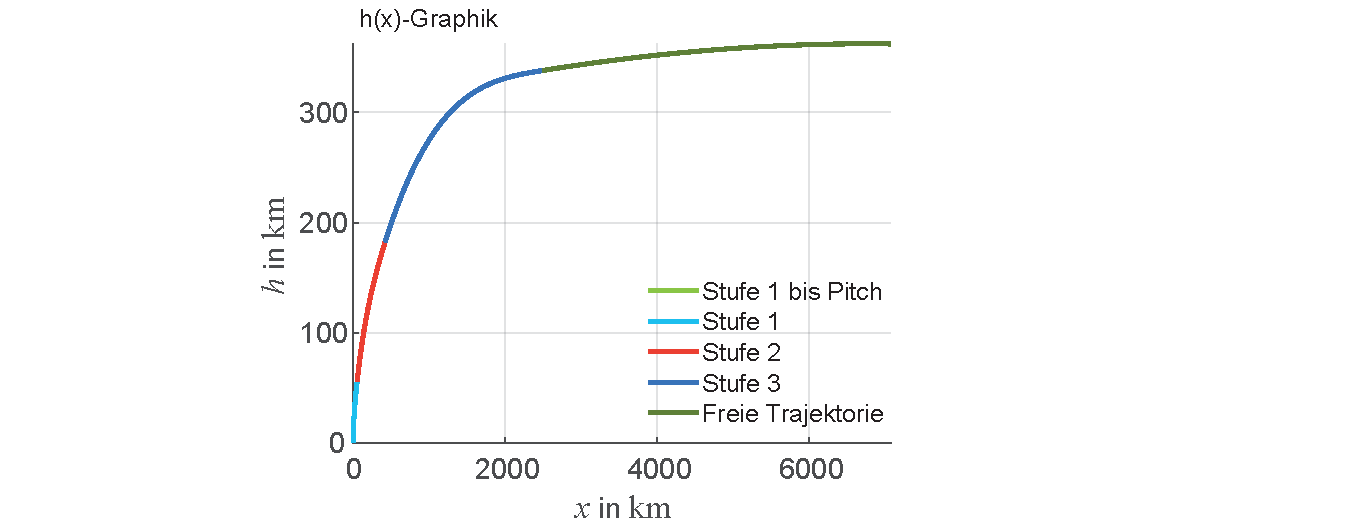
\includegraphics[width=\textwidth]{Startkurve.pdf} 
	\caption[Trajektorie nach Start von der Erdoberfl�che.]{Trajektorie nach Start von der Erdoberfl�che. Parameter siehe \mladynref{Raketenstart2Orbit02.m}.}
	\label{abb:adyn_launch_lsg02}
\end{figure}

\begin{figure}[H]
	\includegraphics[width=\textwidth]{Raketenstart2OrbitUebersicht.pdf} 
	\caption[Geschwindigkeit, Bahnh�he, FPA und Masse nach Start von der Erdoberfl�che. ]{Geschwindigkeit, Bahnh�he, FPA und Masse nach Start von der Erdoberfl�che f�r eine dreistufige Rakete bis zum �bergangspunkt (hier mit $h_\text{T} = \ca \SI{350}{\km}$ angenommen. Parameter siehe \mladynref{Raketenstart2Orbit02.m}.}
	\label{abb:adyn_launch_lsg03}
\end{figure}

\subprob{Startfenster (Launch Window) und  Startrichtung (Startazimut)}

Bisher haben wir uns nur mit der Dynamik und den energetischen Fragen eines Starts von der Erdoberfl�che und des anschlie�enden Transfer in eine gew�nschte Umlaufbahn besch�ftigt, nicht aber mit den Fragen nach der Zeit und den r�umlichen-geometrischen Bedingungen. Man k�nnte nat�rlich prinzipiell das Raumschiff zu jedem beliebigen Zeitpunkt starten und es auch an einen beliebigen Ort schie�en, um dann mit verschiedenen Bahnman�ver die Zielbahn zu erreichen. Aber das w�re eine enorme Verschwendung von Treibstoff. 

Unter einem Startfenster verstehen wir den Zeitraum, in welchem ein Raumschiff direkt in den gew�nschten Orbit \bzw auf eine geeignete Transferbahn (siehe vorhergehenden Abschnitt) gestartet werden kann. Dazu m�ssen wir abh�ngig vom gew�nschten Orbit und der geographischen Position des Abschussortes eine geeignet Startzeit und einen geeigneten Startwinkel finden. 

Hierbei gilt es zwei F�lle zu unterscheiden, zum einen, wenn die Inklination der gew�nschten Bahn $i$ gr��er oder gleich der geographischen Breite $\varphi_0$ des Startplatzes ist und zum anderen, wenn die Bahnneigung kleiner als die geographischen Breite ist. Wir werden sehen, dass es im zweiten Fall M�glichkeit gibt, direkt in den Orbit zu starten. 

Ein geeigneter Startzeitpunkt ist gegeben, wenn sich der Startort in der Position der Sternzeit des Startfensters (LWST) befinden, wobei  �in Position� hei�t, dass sich  Startplatz (bzw genauer der Breitenkreis des Startorts) und die gew�nschte Bahnebene schneiden. Wir betrachten dazu das sph�rische Dreieck in \figref{adyn_launch_lsg02}, welches durch drei Linien/Seiten gegeben ist. Die erste Seite ergibt sich aus der Bodenspur f�r die Umlaufbahn, die zweite aus der �quatorlinie und die dritte aus dem L�ngenkreis des Startplatzes. 
Aus \figref{adyn_launch_lsg02} entnehmen wir ferner noch weitere Gr��en mit folgenden Definitionen und Beziehungen:\\

\begin{tabular}[h]{ll}
LWST &~Sternzeit des Startfenster\index{Startfenster} (Launch Window Siderial Time)\index{Launch Window Siderial Time}\\
$\delta$ &~Hilfswinkel in Startrichtung\\
$\theta$ &~Standortwinkel des Startfensters\\
$\beta$  &~Startazimut\index{Startazimut}\\
$\Omega$ &~Rektaszension des aufsteigenden Knotens\\
\end{tabular}

\begin{figure}[H]
	\includegraphics[width=\textwidth]{BestimmungLWST.pdf} 
	\caption[LST und sph�risches Dreieck zur Bestimmung des LWST.]{LST \fa und sph�risches Dreieck zur Bestimmung des LWST \fb.}
	\label{abb:adyn_launch_lsg04}
\end{figure}

Mit dem Winkelkosinussatz der sph�rischen Trigonometrie \cite{Meyers1995} $~\cos \alpha = -\cos\beta\,\cos\gamma\,+\,\sin\beta\,\sin\gamma\,\cos a$ 
finden wir 
\begin{align*}
\cos i = -\cos(\pi/2)\,\cos\delta\,+\,\sin(\pi/2)\,\sin\delta\,\cos \varphi_0\,,
\end{align*}
was sich mit $\cos(\pi/2) = 0$ und $\sin(\pi/2) = 1$ zu
\begin{align}
\sin \delta = \cos i / \cos \varphi_0\, \label{eq:adyn_launch_lsg04}
\end{align}
vereinfacht. F�r das rechtwinklige sph�rische Dreieck gilt au�erdem \cite{Meyers1995}: $\cos \delta = \cos \theta \,\sin i~$, 
woraus schlie�lich mit \eqref{eq:adyn_launch_lsg03}
\begin{align}
\cos \theta = \frac{\cos \delta }{\sin i} = \frac{\sqrt{1 - \sin^2\delta}}{\sin i} = \frac{\sqrt{\lk 1 - \cos^2 i / \cos^2 \varphi_0 \rk}}{\sin i}
\label{eq:adyn_launch_lsg05}
\end{align}
folgt. F�r die n�rdliche Hemisph�re ergibt sich damit das LWST zu:
\begin{align}
\text{In der N�he des aufsteigenden Knotens: ~~~}\mathrm{LWST}_\text{auf} &= \Omega + \theta ~\,, \label{eq:adyn_launch_lsg06} \\
\text{In der N�he des absteigenden Knotens: ~~~~}\mathrm{LWST}_\text{abs} &= \Omega + (180\degree - \theta) \,. \label{eq:adyn_launch_lsg07}
\end{align}

\begin{figure}[H]
	\includegraphics[width=\textwidth]{StartAzimute.pdf} 
	\caption[Startazimut.]{Startazimut in der N�he des \fa aufsteigenden Knotens und des \fb absteigenden Knotens.}
	\label{abb:adyn_launch_lsg05}
\end{figure}

Es gibt noch einen letzten Winkel, der ber�cksichtigt werden muss, n�mlich das Startazimut $\beta$, \dh die Richtung in die gestartet werden soll. Dies ist der Winkel zwischen dieser �Aufw�rts�-Richtung und der Startrichtung (\figref{adyn_launch_lsg03}) und wird von der Nordrichtung aus im Uhrzeigersinn gemessen. Er ist vom Betrag her gleich dem Winkel $\delta$, womit wir schreiben k�nnen:
\begin{align}
\beta = \arcsin \frac{\cos i}{\cos \varphi_0}\,. \label{eq:adyn_launch_lsg08}
\end{align}
Wir erkennen an dieser Beziehung auch, dass die erreichbare Neigung der Bahn immer gr��er als die geographische Breite des Startortes sein muss, andernfalls w�rde $\beta$ komplexe Werte annehmen. Es gilt also immer $i \geq \varphi_0$, wobei die minimal Bahnneigung bei einem Startazimut von $90\degree$ (entspricht Ost) erreicht wird (\figref{adyn_launch_lsg04}).\\
F�r ein gegebenes $\Omega$ der Bahn gibt es  zwei L�sungen oder Startzeiten pro Rotation. Bei jeder davon kann man dann zwischen prograden und retrograden Umlaufbahnen w�hlen. Diese werden entlang der berechneten Startazimute in Richtung Norden oder S�den verlaufen, wobei die Startfenster einige Zeit auseinander liegen. Es gibt nur eine L�sung, wenn die Neigung genau dem Breitengrad entspricht.  Wir wolle zwei Beispiele angeben (siehe auch \mscr~\mladynref{Raketenstart2Orbit03.m}).

\begin{figure}[H]
	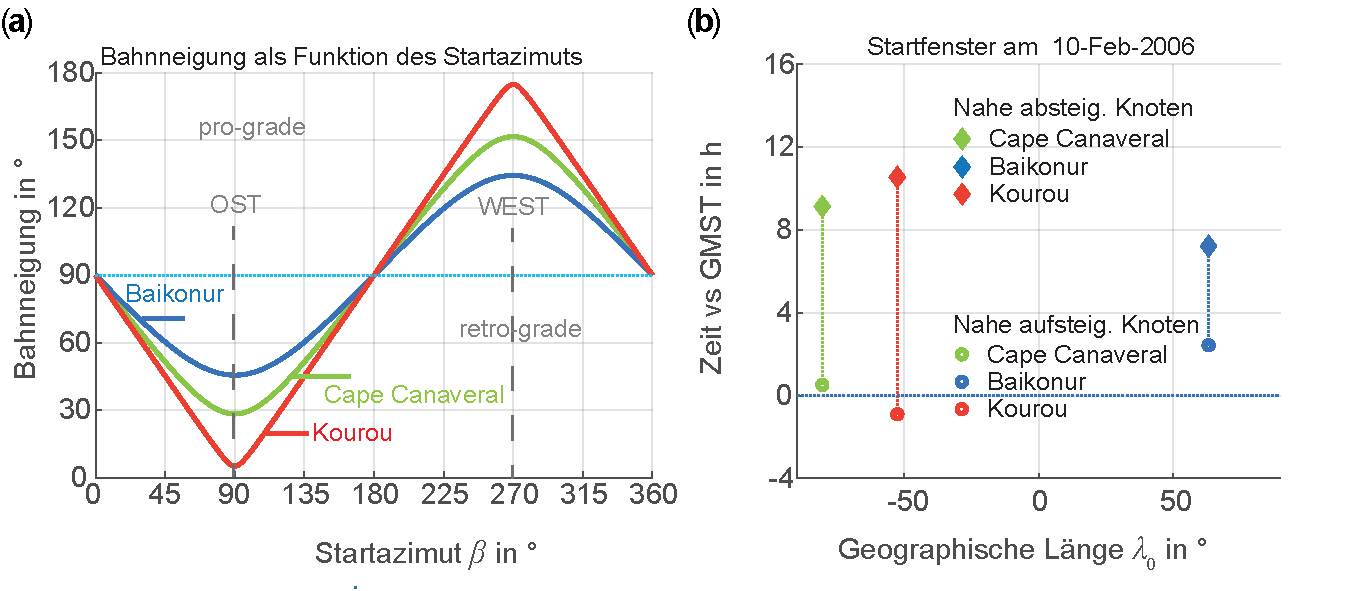
\includegraphics[width=\textwidth]{StartAzimuteStartFenster.pdf} 
	\caption[Bahnneigung und Startfenster als Funktion des Startazimuts und Startfenster zur ISS.]{Bahnneigung \fa und Startfenster \fb als Funktion des Startazimuts f�r verschiedene Weltraumzentren.}
	\label{abb:adyn_launch_lsg06}
\end{figure}

Die Internationale Raumstation umkreist die Erde mit einer Neigung von $51.6\degree$. F�r einen Start von Cape Canaveral (Breitengrad $28.383\degree$) \bzw vom Kosmodrom Baikonur (Breitengrad 45.617�) in die ISS-Umlaufbahn berechnen sich die Startazimute zu:
ergibt sich dann:
\begin{align*}
\beta_\text{CC}  &= \arcsin \frac{\cos(51.6\degree)}{\cos(28.383\degree)} = 44.98\degree~~ \text{\bzw}~~135.02\degree\,,\\ 
\beta_\text{Bai} &= \arcsin \frac{\cos(51.6\degree)}{\cos(45.617\degree)} = 63.21\degree~~ \text{\bzw}~~116.80\degree\,. 
\end{align*}

Die Berechnung der  Startfenster und Startazimute f�r die ISS f�r den 10. M�rz 2006 ist im \mscr~\mladynref{Raketenstart2Orbit03.m}\, ausgef�hrt.
F�r die ISS haben wir daf�r folgende Bahnparameter f�r Anfang 2006 benutzt \cite{JPL2020}.\\

\begin{tabular}{L{7cm}C{2cm}L{4cm}}
Epoche & $t_\text{epoch}$ & 09.02.2006 20:26:00.0000\\
Inklination &$i$ & $51.6448\degree$\\
Rektaszension des aufsteigenden Knotens & $\Omega$ & $122.3522\degree$\\
numerische Exzentrizit�t der Umlaufbahn & $e$ & 0.0008835\\
Argument des Perig�ums & $\omega$ &$257.3473\degree$\\
Mittlere Anomalie & $M$ & $251.7436\degree$\\
Mittlere Bewegung & $n$ & $ \SI{15.74622749}{\per\day}$\\
\end{tabular}
\medskip

Die Sternzeit in Greenwich bestimmt man aus dem Julianischen Datum JD f�r den Zeitpunkt 0:00 h UTC. Zun�chst berechnet man das Julianische Datum in Jahrhunderten seit dem 1.1.2000. 
	\[ T\,=\,\frac {JD-2451545.0}{36525} \]
und daraus die mittlere Sternzeit f�r Greenwich f�r den Zeitpunkt 0:00 h UTC:
\begin{align}
\mathrm {GMST_0} \,&=\,6^{\mathrm {h} }41^{\mathrm {m} }50.54841^{\mathrm {s}}\,+\,8640184.812866^{\mathrm {s} }\, T\,+\,0.093104^{\mathrm {s} }\, T^{2}\,-\,0.0000062^{\mathrm {s} }\, T^{3}\\
&=\,24110.54841^{\mathrm {s} }+8640184.812866^{\mathrm {s} }\, T \, + \,0.093104^{\mathrm {s} }\, T^{2}\,-\,0.0000062^{\mathrm {s} }\, T^{3}\\
&=\,100.46061837\degree+36000.770053608\degree\, T\,+\,0.000387933\degree\, T^{2}\,-\,(T^{3}/38710000)\degree
\end{align}
F�r einen Beobachter auf der geographischen L�nge $\lambda_0$ muss man die Sternzeit noch auf seine Ortssternzeit LST umrechnen:
\begin{align}
\mathrm {LST} \,&\,=\mathrm {GMST} +\lambda~~~{\text{f�r GMST im Gradma�}}
\end{align}

Wir verweisen auf das \mscr~\mladynref{Raketenstart2Orbit03.m} und auch auf \kap{hm_zeitdefinition}.


\subprob{Berechnung der 3D-Trajektorien im Inertialsystem}


F�r die weiteren Berechnungen muss man ber�cksichtigen, das wir alle Gr��en wie \zb das in \eqref{eq:adyn_launch_lsg08} abgeleitete Startazimut im Inertialsystem berechnet hatten. Da wir jedoch die Rakete von der rotierenden Erdoberfl�che starten, muss man die Erddrehung entsprechend ber�cksichtigen, was zu einer leichten Korrektur des Startazimuts und auch des Geschwindigkeitsbudgets f�hrt. Wir wollen ab sofort zur besseren Unterscheidung die Gr��en im mitbewegten System gestrichen kennzeichnen, die im Inertialsystem als ungestrichen.
So ist \zb f�r eine Umlaufbahn von 300 km H�he das Mindestgeschwindigkeitsbudget $\Delta \vec{v}$ (ohne Reibung und Reserven) durch $\Delta \vec{v} = \Delta v\,(\sin \beta\,\veceX + \cos \beta\,\veceY)$ mit $\Delta v = \SI{7.7309}{\km\per\second}$ gegeben, wobei die Einheitsvektoren in der Bahnebene liegen und in die Ost- \bzw Nordrichtung zeigen. Am einfachsten macht man sich nun an Hand von \figref{adyn_launch_lsg07} klar, dass zur Berechnung des Geschwindigkeitsbudget $\Delta \vec{v}'$ im Nichtinertialsystem die vektorielle Differenz von $\Delta \vec{v}$ und $\Delta v_\text{E,t}\,\veceX = \SI{0.465}{\km\per\second}\,\cos\phi_0$ (\vgl \eqref{eq:adyn_launch10}) gebildet werden muss. Man erh�lt:
\begin{align}
\Delta v' = \Delta v \, \sqrt{\lk \sin \beta \, - \Delta v_\text{E,t}/ \Delta v \rk^2 + \cos^2 \beta}\,. \label{eq:adyn_launch_lsg09}
\end{align}
Das Startazimut im mitbewegten System $\beta'$ ergibt sich dann zu:
\begin{align}
\beta' = \arctan \lk \frac{\Delta v\,\sin \beta\, - v_\text{E,t}}{\Delta v\,\cos \beta\,} \rk\,. \label{eq:adyn_launch_lsg10}
\end{align}
F�r einen Start zur ISSS von Cape Canaveral �ndert es sich beispielsweise von $44.98\degree$ auf $42.76\degree$. Auch der FPA rechnet sich enstprechend um zu:
\begin{align}
\gamma = \arcsin \lk \frac{\Delta v'}{\Delta v}\,\sin \gamma' \rk\,. \label{eq:adyn_launch_lsg11}
\end{align}

\begin{figure}[H]
	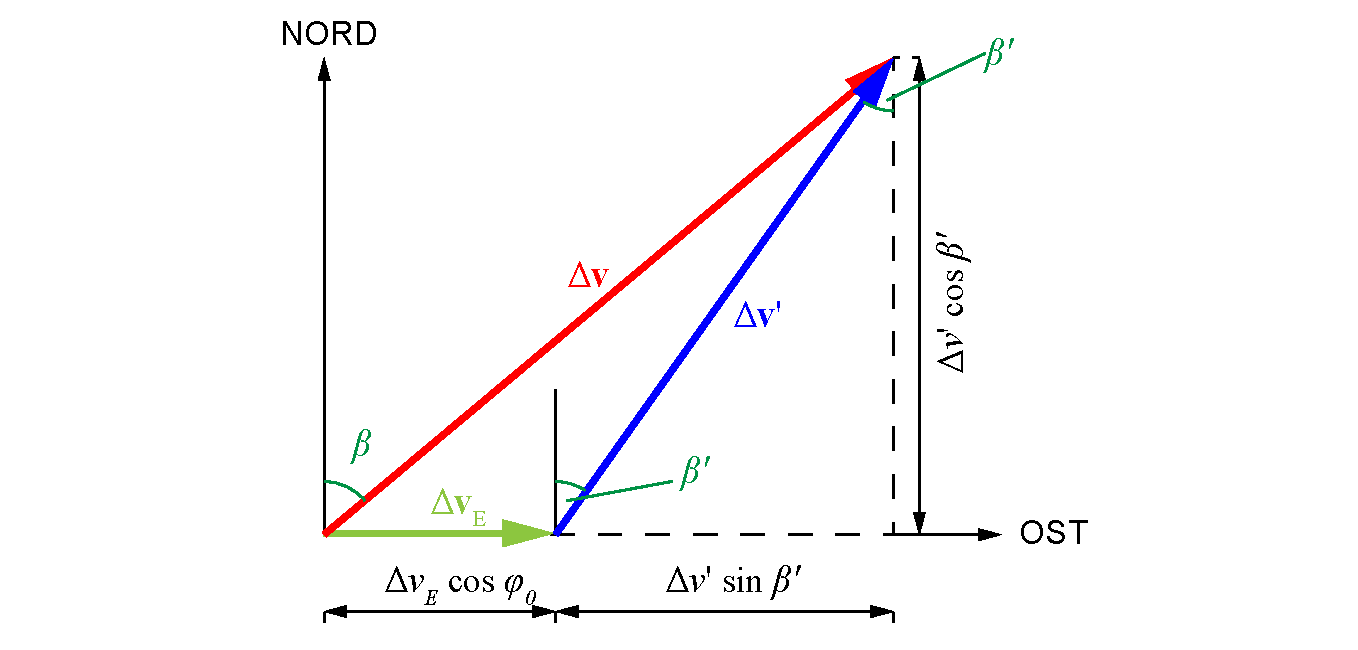
\includegraphics[width=\textwidth]{StartAzimutInertial.pdf} 
	\caption[Ber�cksichtigung der Erdrotation beim Start von Raketen.]{Ber�cksichtigung der Erdrotation beim Start von Raketen.}
	\label{abb:adyn_launch_lsg07}
\end{figure}

F�r die Berechnung der 3D-Trajektorien haben wir drei M�glichkeiten:
\begin{enumerate}[a)]
	\item Wir betrachten alles im geozentrisch-raumfesten Inertialsystem und l�sen numerisch die Bewegungsgleichung \eqref{eq:adyn_launch_vec} in 3 Dimensionen. Dabei m�ssen wir bei den Anfangsbedingungen die von der Rakete mitgenommene Rotation der Erde nach \eqref{eq:adyn_launch_lsg09} ber�cksichtigen, ebenso wie das umgerechnete Startazimut $\beta$ und den Anfangs-FPA $\gamma_0$ nach \eqref{eq:adyn_launch_lsg10} \bzw \eqref{eq:adyn_launch_lsg11}. Man beachte, dass die beiden Gr��en im topozentrischen System definiert sind und mit den Ortskoordinaten des Startorts in das Inertialsystem umgerechnet werden m�ssen.\\
	Bei der Berechnung der Reibung muss man ber�cksichtigen, dass die Atmosph�re mitrotiert und folglich die f�r die Reibung ma�gebliche aktuelle Geschwindigkeit $v'$ aus der im Inertialsystem geltenden Geschwindigkeit in $v$ umgerechnet werden muss:
\begin{align}
\begin{split}
		\vec{v}'(t) &= \vec{v}(t) - \vec{v}_\text{E,0} ~~~\text{mit}~~~\vec{v}_\text{E,0} = \vec\omega_\text{E} \times \vec{r}_0 \,.
\end{split} \label{eq:adyn_launch_lsg12}
\end{align}
Die Bewegungsgleichung lautet also:
\begin{align}
\begin{split}
		\vec{\ddot{r}}\begin{pmatrix} \ddot{x}\\ \ddot{y} \\ \ddot{z} \end{pmatrix} &=  \frac{\vec{F}_\text{S}(t) + \vec{F}_\text{G}(t) - \vec{F}_\text{D}(t)}{m_\text{R}(t)} = 
		\frac{F_\text{S}(t)}{m_\text{R}(t)\,v(t)} \begin{pmatrix} \dot{x}\\ \dot{y} \\ \dot{z} \end{pmatrix} 
 - \frac{G\,M_\text{E}}{\left| \vec{r}(t) \right|^3} \begin{pmatrix} x \\y\\z \end{pmatrix}
 - \frac{\varrho(r)\, v'\, A \,c_\text{D}}{m_\text{R}(t)} \begin{pmatrix} \dot{x}'\\ \dot{y}'\\ \dot{z}' \end{pmatrix}\,.
\end{split} \label{eq:adyn_launch_lsg13}
\end{align}
Die Nickkorrektur wird wie folgt berechnet:\\ 
Nach Bestimmung der Geschwindigkeit zum Zeitpunkt kurz vor der Nickkorrektur $\vec{v}(t=t_\text{Nick-})$, die sich ohne der mitgenommenen
Rotation der Erde ergibt (also nur die Geschwindigkeitszunahme durch den Schub), erfolgt 
die Drehung des Geschwindigkeitsvektors/Schubvektors um den Nickwinkel $\gamma_\text{N}$ in Richtung des Startazimuts. Diese Drehung wird im Horizontsystem 
mit folgender Drehmatrix $\mathbb{R}_\text{Nkorr}$ beschrieben, wobei hierbei zuerst die
Nickkorrektur und dann die Ausrichtung auf das Azimut ausgef�hrt wird. Die dazu notwendigen Berechnung der Drehmatritzen f�hren wir in einer Nebenrechnung aus:

\begin{nebenrechnungNeu} {Einheitsvektoren und Transformationsmatrix}

\begin{align*}
    \vec{r} &= r\,\begin{pmatrix} \sin\theta\,\cos\phi \\ \sin\theta\,\sin\phi \\ \cos\phi \end{pmatrix} ~~ \text{\bzw in geograph. Koord.}~~~ \vec{r} = r\,\begin{pmatrix} \cos\varphi\,\cos\lambda \\ \cos\varphi\,\sin\lambda \\ \sin\varphi \end{pmatrix}\\
    \vec{e}_\text{r} &= \frac{\d\vec{r}}{\d r} \;= \;\begin{pmatrix} \sin\theta \,\cos\phi \\ \sin\theta\,\sin\phi \\ \sin\phi \end{pmatrix}\; \widehat{=} \;\begin{pmatrix} \cos\varphi\,\cos\lambda \\ \cos\varphi\,\sin\lambda \\ \sin\varphi \end{pmatrix}\\
     \vec{e}_\theta &= \frac{1}{r}\,\frac{\d\vec{r}}{\d \theta}\;=\; \begin{pmatrix} \cos\theta \,\cos\phi \\ \cos\theta \,\sin\phi \\ -\sin\phi \end{pmatrix}\;\widehat{=}\;\vec{e}_\varphi = \frac{1}{r}\,\frac{\d\vec{r}}{\d \varphi}\;=\; \begin{pmatrix} -\sin\varphi \,\cos\lambda \\ -\sin\varphi\,\sin\lambda \\ \cos\varphi \end{pmatrix} \\
     \vec{e}_\phi &= \frac{1}{r\,\sin\theta}\,\frac{\d\vec{r}}{\d \phi}\;=\; \begin{pmatrix} -\sin\phi\\ \cos\phi \\ 0 \end{pmatrix}\;\widehat{=}\;\vec{e}_\lambda = \frac{1}{r\,\cos\varphi}\,\frac{\d\vec{r}}{\d \lambda}\;=\; \begin{pmatrix} -\sin\lambda \\ \cos\lambda\\ 0 \end{pmatrix} \\
    \rightarrow \mathbb{S} &= \lk \vec{e}_\text{r},\,\vec{e}_\theta,\,\vec{e}_\phi \rk \;=\; \begin{pmatrix} \cos\varphi\,\cos\lambda & -\sin\phi\,\cos\varphi & -\sin\lambda \\ \cos\varphi\,\sin\lambda & -\sin\varphi\,\cos\lambda & \cos\lambda \\ \sin\varphi & \cos\varphi& 0 \end{pmatrix}
\end{align*}

\end{nebenrechnungNeu}

Wir erhalten damit:

\begin{align}
\begin{split}
		\mathbb{R}_\text{Nkorr} &= \mathbb{R}_\text{A}\, \mathbb{R}_\text{N} ~~\text{mit}~~\\
		\mathbb{R}_\text{N} &= \begin{pmatrix} \cos\gamma_\text{N} & ~~-\sin\gamma_\text{N} & ~~0 \\
		                                      \sin\gamma_\text{N} & ~~+\cos\gamma_\text{N} & ~~0 \\
																					0 & 0 & 1\end{pmatrix}\ ~~\text{und}~~
		\mathbb{R}_\text{A} = \begin{pmatrix} 1 &~~ 0 &~~ 0 \\
		                                      0 &~~\cos\beta' & ~~-\sin\beta'\\
		                                      0 &~~\sin\beta' & ~~+\cos\beta' \end{pmatrix}\,.
\end{split} \label{eq:adyn_launch_lsg14}
\end{align}
Die so berechnete Drehmatrix geht jedoch davon aus, dass die Rakete vor der
Nickkorrektur entlang der $x$-Richtung der Drehmatrix ausgerichtet ist. In unserem Fall ist die Rakete aber radial nach au�en gerichtet. Daher muss die Drehmatrix noch
in das richtige (sph�rische) Koordinatensystem transformiert werden. (Siehe auch \mscr~\mladynref{KOS.m}):
\begin{align}
\begin{split}
  \mathbb{R}_\text{Nkorr}' &= \mathbb{S} \,\mathbb{R}_\text{Nkorr}\, \mathbb{S}^\text{T}~~~\text{mit}~~~\\
	\mathbb{S} &= \begin{pmatrix} \vec{e}_r  & \vec{e}_\varphi &\vec{e}_\lambda \end{pmatrix} =
	              \begin{pmatrix} \cos\varphi\,\cos\lambda &~~ -\sin\varphi\,\cos\lambda &~~ -\sin\lambda\\
			                          \cos\varphi\,\sin\lambda &~~ -\sin\varphi\,\sin\lambda &~~ +\cos\lambda\\
			                          \sin\varphi)                &~~ +\cos\varphi                &~~ 0 \end{pmatrix}\,.
\end{split} \label{eq:adyn_launch_lsg15}
\end{align}
Der Geschwindigkeitsvektor (zugleich die Schubrichtung) der Rakete nach Nickkorrektur ist dann:
\begin{align*}
\vec{v}(t=t_\text{Nick+})  = \mathbb{R}_\text{Nkorr}'\,\vec{v}(t=t_\text{Nick-})\,.
\end{align*}
Wir bestimmen die H�he, den FPA, die Geschwindigkeit und die Masse der Rakete f�r die einzelnen Stufen bis die Rakete einen FPA von 0 hat. Dann erfolgt nur noch ein tangentialer Schub bis zum Erreichen der notwendigen Kreisbahngeschwindigkeit. 

Das Ergebnis der Rechnungen ist in \figref{adyn_launch_lsg08} und \figref{adyn_launch_lsg09} dargestellt und im \mscr~\mladynref{Raketenstart2Orbit04.m} ausgef�hrt und ausf�hrlich erl�utert.

\begin{figure}[H]
	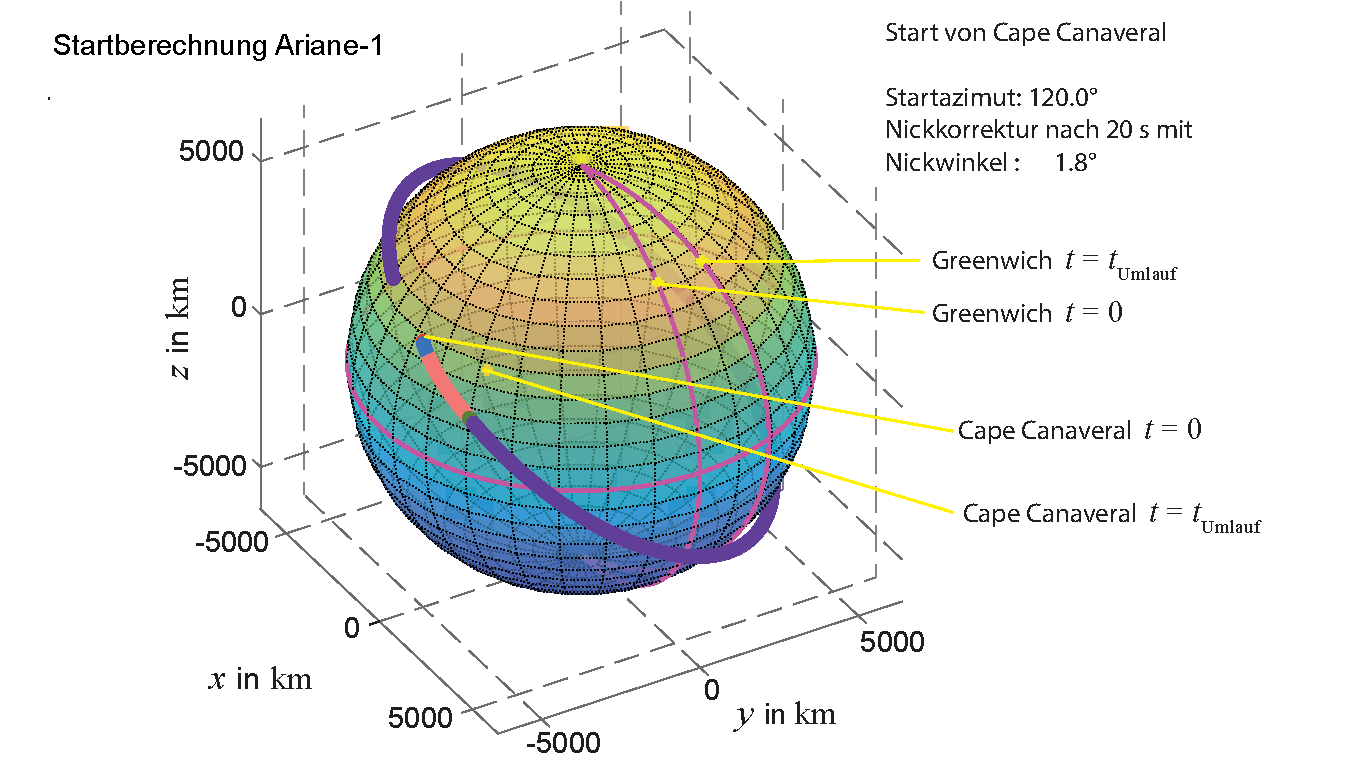
\includegraphics[width=\textwidth]{StartAriane01.pdf} 
	\caption[Trajektorie nach Start von der Erdoberfl�che.]{Trajektorie nach Start von der Erdoberfl�che. Parameter siehe \mladynref{Raketenstart2Orbit04.m}.}
	\label{abb:adyn_launch_lsg08}
\end{figure}

\begin{figure}[H]
	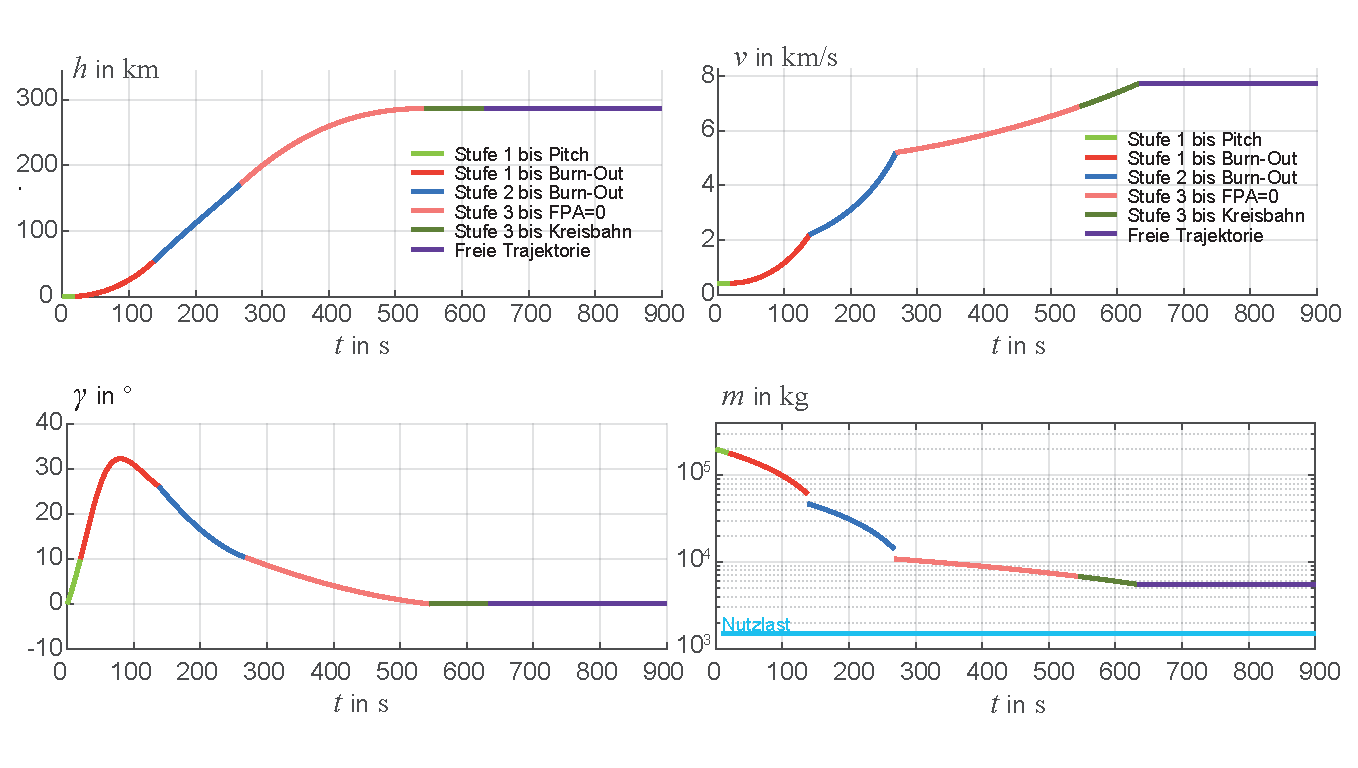
\includegraphics[width=\textwidth]{StartAriane02.pdf} 
	\caption[H�he, FPA,  Geschwindigkeit und  Masse der Ariane 1 nach Start von der Erdoberfl�che.]{H�he, FPA,  Geschwindigkeit und  Masse der Ariane 1 nach Start von der Erdoberfl�che. Parameter siehe \mladynref{Raketenstart2Orbit04.m}.}
	\label{abb:adyn_launch_lsg09}
\end{figure}

\item Als Alternative kann man die Trajektorien nat�rlich auch im mitbewegten \KOS des Beobachters im Horizontsystem berechnen. Das f�hrt auf �hnliche Rechnungen wie wir im Kap. 1.3.2 im Band I (Physik Bewegung) zum Wurf und freien Fall auf der Erdoberfl�che gemacht hatten.
\item Als weitere Alternative k�nnen wir nat�rlich das Ergebnis der Rechnungen im mitbewegten \KOS (Siehe Teilaufgabe 2) benutzen und ins Inertialsystem transformieren. Zwei Ortsvektoren sind dabei ausgezeichnet: Der Vektor zum Startpunkt und der Vektor zum aufsteigenden Knoten. Die Inklination und der aufsteigende Knoten der Bahn sind durch Startazimut, Startfenster und geographische Position des Startortes gegeben. Die Transformation erfolgt �ber die im \kap{hm_bahnen_hk_PQR} hergeleiteten Matrizen.\\
Wir empfehlen dem Leser zur Vervollst�ndigung des Bildes beide Alternativen selbst zu rechnen.
\end{enumerate}

\end{subprobs}
\end{sol} 
\textcolor{blue} {$\rightarrow$ zur} \probref{adyn_launch01}.\\
\noindent\rule[1ex]{\textwidth}{0.5pt}  \newpage  \clearpage

%-----------------------------------------------------------------------------------------------------------

\begin{sol}{prob:adyn_reentry01}\label{lsg:adyn_reentry01} %�bung27
\textbf{Parameter des Wiedereintritts in die Erdatmosph�re}\\

\begin{figure}[H]
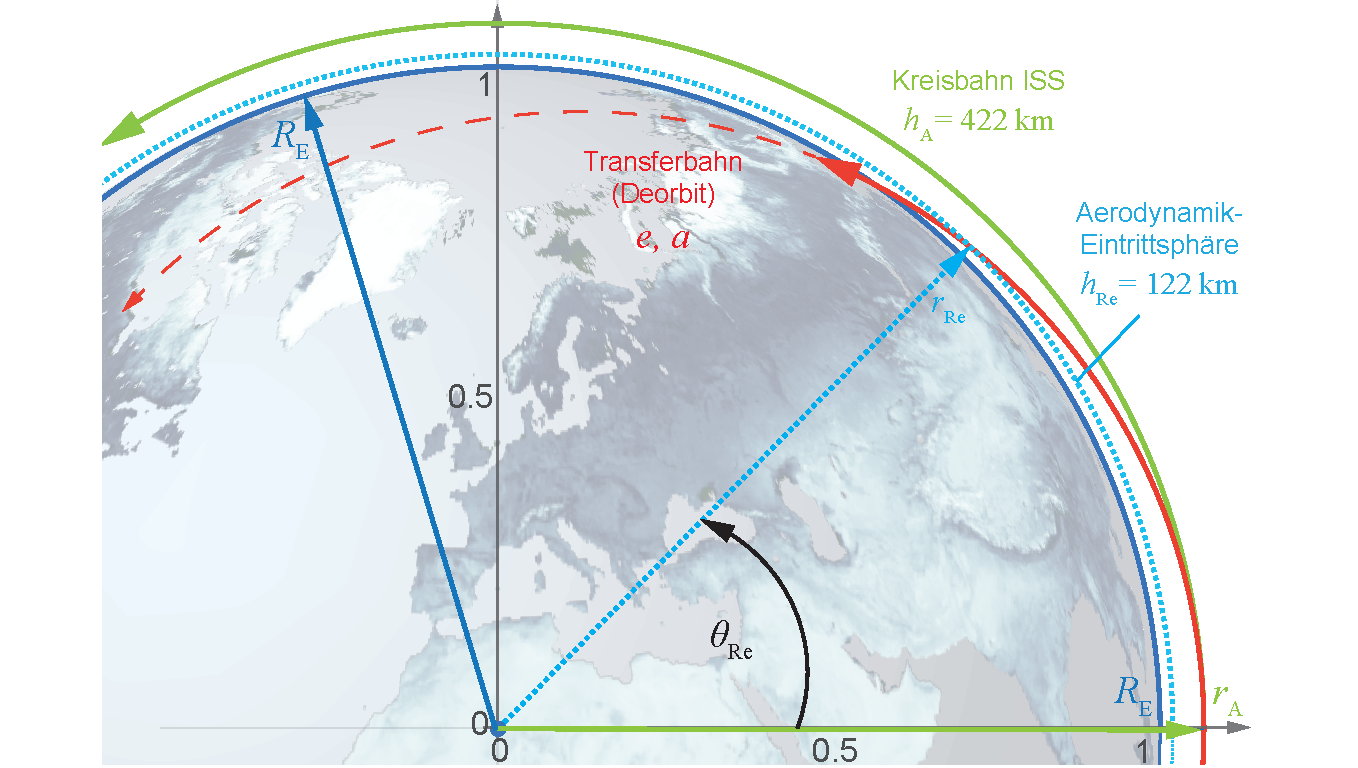
\includegraphics[width=\textwidth]{ReentryGeometrie01.pdf}
\caption[Geometrie des Wiedereintritts in die Erdatmosph�re.]{Geometrie des Wiedereintritts in die Erdatmosph�re. Siehe auch \mscr~\mladynref{Transfer2Reentry.m} f�r weitere Details und Graphiken.}
\label{abb:adyn_reentry_geometrie01}
\end{figure}

\begin{figure}[H]
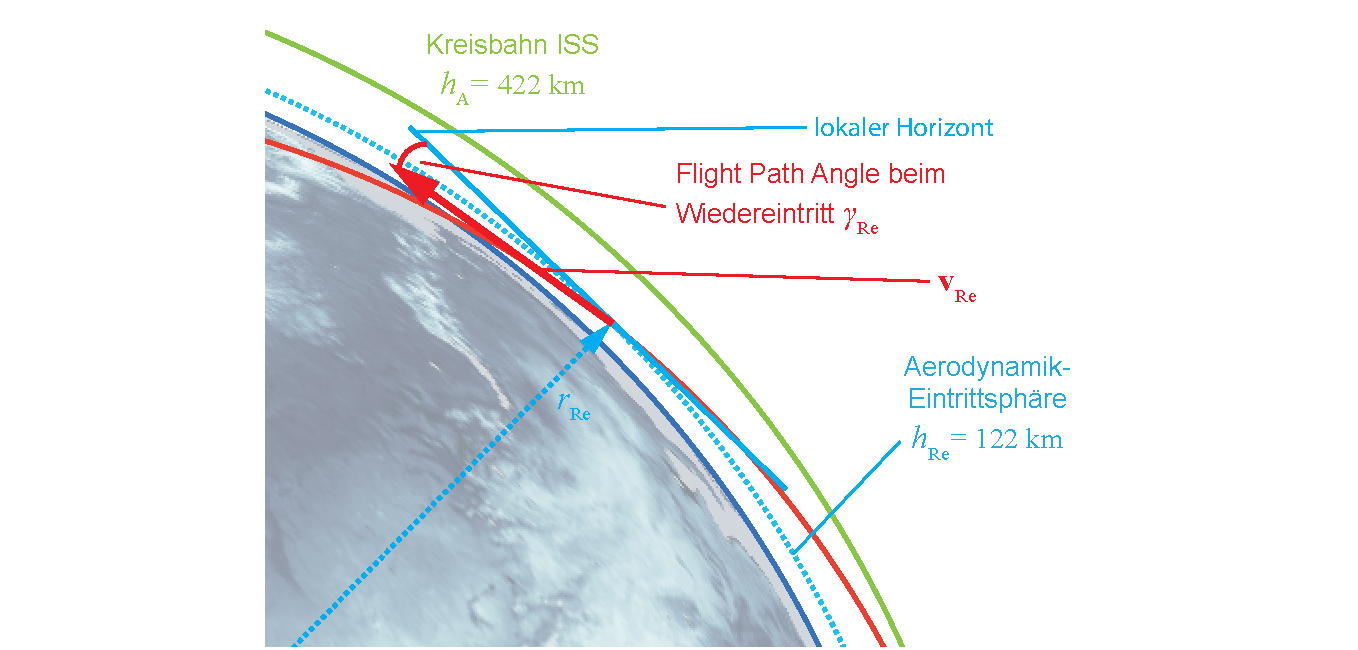
\includegraphics[width=\textwidth]{ReentryGeometrie02.pdf}
\caption[Geometrie des Wiedereintritts in die Erdatmosph�re.]{Geometrie  (Detail) des Wiedereintritts in die Erdatmosph�re. Siehe auch \mscr~\mladynref{Transfer2Reentry.m} f�r weitere Details und Graphiken.}
\label{abb:adyn_reentry_geometrie02}
\end{figure}

%\begin{nebenrechnung}
%\begin{align*}
    %e &= \frac{q^2-\lk 2q-1\rk\,\cos^2\gamma_\text{Re}}{q^2-\cos^2\gamma_\text{Re}} = \frac{q^2-\lk 2q-1\rk\,u^2}{q^2-u^2} \\
    %\cos\theta_\text{Re} &= q\,\frac{\lk 1-e\rk}{e}-\frac{1}{e} = \frac{q-1}{e}-q = \frac{Z}{N}\\
    %&= \frac{\lk q-1\rk\lk q^2-u^2\rk-q\,\lk q^2-\lk 2q-1\rk\,u^2\rk}{q^2-\lk2q-1\rk\,u^2}\\
    %N &= q^2-2\,q\,u^2+ u^2 = q^2-2q+1+2q-1-2\,q\,u^2+u^2\\
    %&= \lk q-1\rk^2 +\lk 2q-1\rk - \lk 2q-1\rk\,u^2 \\
    %&= \lk q-1\rk^2 + \lk2q-1\rk\lk1-u^2\rk \\
    %&= \hat{q}^2 + \lk 2q-1\rk\,\sin^2\gamma_\text{Re}\\
    %Z &=  \cancel{q^3} - \cancel{q\,u^2}-q^2+u^-\cancel{q^3} +2\,q^2\,u^2-\cancel{q\,u^2} = 2\,q^2\,u^2- 2\,q\,u^2 - q^2+u^2 \\
    %&= \lk q^2-2q+1\rk\,u^2 - \lk q^2-q^2\,u^2\rk = \hat{q}^2\,u^-q^2\,\lk1-u^2\rk\\
    %&= \hat{q}^2\,\cos^2\gamma_\text{Re} - q^2\,\sin^2\gamma_\text{Re}
%\end{align*}
%\end{nebenrechnung}

Wir haben die Geometrie des Deorbits in \figref{adyn_reentry_geometrie01} und \figref{adyn_reentry_geometrie02} dargestellt.\\
Gegeben sind $v_\text{A}$, $r_\text{A}$, $r_\text{Re}$ und der gew�nschte FPA $\gamma_\text{Re}$, gesucht sind der \anf{Ort} $\upsilon_\text{Re}$ \bzw $\theta_\text{Re}$ des \anf{Eintauchens} in die aerodynamische Zone/Sph�re und die Geschwindigkeit $v_\text{Re}$, die das Raumschiff dort hat. Dazu muss man die Bahnparameter $e$ \bzw $a$ kennen, f�r die gilt: $r_\text{A} = a\,\lk 1+e\rk$.\\
Wir starten mit Ellipsengleichung \eqref{eq:hm_kegelschnitt}:
\begin{align}
    r_\text{Re} = \frac{a\,\lk 1-e^2\rk}{1+e\,\cos\upsilon_\text{Re}} = \frac{a\,\lk1-e^2\rk}{1-e\,\cos\theta_\text{Re}} \,. \label{eq:adyn_lsg_reentry01}
\end{align}
Aus der vis-visa-Gleichung \eqref{eq:hm_vis-viva}, die wir zun�chst vektoriell aufschreiben aufschreiben, k�nnen wir eine Beziehung f�r $v_\text{Re}\lk r_\text{Re},\upsilon_\text{Re}\rk$ ableiten.
\begin{nebenrechnungNeu} {  }

\begin{align*}
   \text{Aus} ~~ \vec{L} \times\,\lk \vec{v}\times \vec{L}\rk &= \vec{v} \,\lk \vec{L}\vec{L}\rk - 			   \underbrace{\vec{L}\,\lk \vec{L}\vec{v}\rk}_{\substack{=0}} = L^2\,\vec{v} ~~
   \text{und}\\
    \vec{e} &= -\frac{1}{\mu}\,\lk \vec{L}\times \vec{v}\rk\,\frac{\vec{r}}{r}\,,~~~~
    \vec{v} = \frac{\mu}{L^2}\,\vec{L}\times\lk\vec{e} + \frac{\vec{r}}{r}\rk~~\text{folgt}\\
    \vec{L}\times \vec{v} &= -\mu\,\lk\frac{\vec{r}}{r}+\vec{e}\rk ~~\rightarrow~~
    \vec{L}\times\lk\vec{v}\times \vec{L}\rk = \vec{L}\times\mu\,\lk\frac{\vec{r}}{r} + \vec{e}\rk\,, \\
    L^2\,\vec{v} &= \mu\,\lek\vec{L}\times \lk\vec{e} + \frac{\vec{r}}{r}\rk\rek ~~\rightarrow~~~
    \vec{v} = \frac{\mu}{L^2}\lek \vec{L}\times\lk \vec{e}+ \frac{\vec{r}}{r}\rk\rek\,, \\
    \rightarrow~~~|\vec{v}| &=\frac{\mu}{L^2}\,\sqrt{\lek \vec{L}\times\lk \vec{e}+\frac{\vec{r}}{r}\rk\rek\lek\vec{L}\times\lk \vec{e}+\frac{\vec{r}}{r}\rk\rek}\,.\\
\text{Wegen}~~&\lk \vec{a}\times \vec{b}\rk\lk \vec{a}\times\vec{b}\rk = a^2\,b^2 -\lk a\,b\rk^2~~\text{folgt:}\\
    |\vec{v}| &= \frac{\mu}{L^2}\,\sqrt{L^2\,\lk \vec{e} + \frac{\vec{r}}{r}\rk^2 - \underbrace{\lek \vec{L}\,\lk \vec{e} + \frac{\vec{r}}{r}\rk\rek^2 }_{=0}}~~~\text{und da}~~~\vec{L} \perp \vec{e},\vec{r} \\
    |\vec{v}| &= \frac{\mu}{L^2}\,L\,\sqrt{\lk \vec{e} + \frac{\vec{r}}{r}\rk^2} = \frac{\mu}{L}\,\sqrt{e^2+2e\,\cos\upsilon_\text{e} +1}
\end{align*}
\end{nebenrechnungNeu}

Damit haben wir als zweite Gleichung:
\begin{align}
    v_\text{e} = \frac{\mu}{L}\,\sqrt{1+e\,\cos\upsilon_\text{Re} + e^2}\,. \label{eq:adyn_lsg_reentry02}
\end{align}
Als dritte Gleichung brauchen wir noch den FPA. Dieser ist gegeben durch den Winkel zwischen Geschwindigkeitsvektor $\vec{v}$ und lokalem Horizont.
Letzterer liegt senkrecht zum Radiusvektor (Abstandsvektor) $\vec{r}$ in der $\vec{r}$\,-\,$\vec{v}$-Bahnebene und stimmt mit der Richtung des Vektors $\vec{e}$ �berein.
Wir bilden das Skalarprodukt:
\begin{subequations}
\begin{align}
    \vec{v}\,\lk \frac{\vec{L}}{L}\times\frac{\vec{r}}{r}\rk &= r\,\dot{\upsilon} =v\,\cos\gamma\,, \label{eq:adyn_lsg_reentry03a}\\
    \vec{v}\,\frac{\vec{r}}{r} &= \dot{r} = \sin\gamma\,. \label{eq:adyn_lsg_reentry03b}
\end{align} \label{eq:adyn_lsg_reentry03}
\end{subequations}
Aus \eqref{eq:adyn_lsg_reentry03a} folgt mit \eqref{eq:adyn_lsg_reentry02} und $L = r^2\,\dot{\upsilon}$:
\begin{subequations}
\begin{align}
    \cos\gamma_\text{Re} = \frac{1+e\,\cos\upsilon_\text{Re}}{\sqrt{1+2e\,\cos\upsilon_\text{Re} + e^2}}\,,\label{eq:adyn_lsg_reentry04a} \\
    \sin\gamma_\text{Re} = \frac{e\,\sin\upsilon_\text{Re}}{\sqrt{1+2e\,\cos\upsilon_\text{Re}+e^2}}\,. \label{eq:adyn_lsg_reentry04b}
\end{align} 
\end{subequations}
Man kann folglich mit \eqref{eq:adyn_lsg_reentry04a} und  \eqref{eq:adyn_lsg_reentry04b} auch die Geschwindigkeit an einem beliebigen Bahnpunkt durch
\begin{align}
\begin{split}
    \vec{v} &= \frac{\mu}{L}
    \begin{pmatrix}
        \sin\gamma \\
        \cos\gamma
    \end{pmatrix}
    =
    \frac{\mu}{L}
    \begin{pmatrix}
        e\,\sin\upsilon \\
        1+e\,\cos\upsilon
    \end{pmatrix} \\
    &= \sqrt{\frac{\mu^{\killA{2}}}{\killA{\mu}\,a\,\lk 1-e^2 \rk}}
    \begin{pmatrix}
        e\,\sin\upsilon \\
        1+e\,\cos\upsilon
    \end{pmatrix} 
    =\sqrt{\frac{\mu}{p}}
     \begin{pmatrix}
        e\,\sin\upsilon \\
        1+e\,\cos\upsilon
    \end{pmatrix} 		
\end{split} \label{eq:adyn_lsg_reentry05}
\end{align}
in der Koordinate $\upsilon$ und den Bahnparametern $p$, $e$ ausdr�cken. \\
Zus�tzlich zu Gleichungen \eqref{eq:adyn_lsg_reentry01}, \eqref{eq:adyn_lsg_reentry02} und \eqref{eq:adyn_lsg_reentry04a} gilt noch $r_\text{A} = a\,\lk1+e\rk$ und $q= r_\text{A}/r_\text{Re} > 1$.
Aus \eqref{eq:adyn_lsg_reentry01} k�nnen wir dann folgende Beziehung ableiten:
\begin{align}
   e\,\cos\upsilon_\text{Re} &= \frac{a\,\lk 1-e^2\rk}{r_\text{Re}} -1 = \frac{a\,\lk 1+e\rk\lk 1-e\rk}{r_\text{Re}} = q\,\lk 1-e\rk-1 \,. \label{eq:adyn_lsg_reentry05a} 
\end{align}
Wir benutzen \eqref{eq:adyn_lsg_reentry05a} in \eqref{eq:adyn_lsg_reentry01} und erhalten:
\begin{align}
\begin{split}
    \cos\gamma_\text{Re} &= \frac{q\,\lk 1-e\rk}{\sqrt{1+2q\,\lk 1-e\rk -2+e^2}}
    = q\,\sqrt{\frac{\lk 1-e\rk^2}{2q-2\,e\,q-1+e^2}}\\
    &= q\,\sqrt{\frac{\lk 1-e\rk^2}{2q-2\,e\,q-\lk 1-e^2\rk}}
    = q\,\sqrt{\frac{\lk 1-e\rk^2}{2q\,\lk 1-e\rk - \lk 1+e\rk\lk1-e\rk}}
    = q\,\sqrt{\frac{1-e}{2q-\lk 1+e\rk}}
\end{split} \label{eq:adyn_lsg_reentry06} 
\end{align}
F�r $v_\text{Re}$ erhalten wir:
\begin{align}
\begin{split}
    v_\text{Re} &= \frac{\mu}{L}\,\sqrt{1+2e\,\cos\upsilon_\text{Re} +e} = \sqrt{\frac{\mu\,\lk 1+2q\,\lk 1-e\rk -1+e^2\rk}{r_\text{A}\,\lk 1-e^2\rk}}\\
    &= \sqrt{\frac{\mu}{r_\text{A}}}\,\sqrt{\frac{2q-2\,q\,e-1+e^2}{\lk 1+e\rk\lk 1-e\rk}} = \sqrt{\frac{\mu}{r_\text{A}}}\,\,\sqrt{\frac{2q\,\cancel{\lk 1-e\rk}}{\lk 1+e\rk\cancel{\lk 1-e\rk}} - \cancel{\frac{\lk 1-e^2\rk}{\lk 1+e\rk\lk1-e\rk}}} \\
    &= \sqrt{\frac{\mu}{r_\text{A}}}\,\sqrt{\frac{2q-\lk 1+e \rk}{\lk 1+e\rk}} = \sqrt{\frac{\mu}{r_\text{A}\,\lk 1+e\rk}}\,\sqrt{2q-\lk 1+e\rk}
\end{split}\label{eq:adyn_lsg_reentry07}
\end{align}
Aus \eqref{eq:adyn_lsg_reentry06} k�nnen wir die Exzentrizit�t $e$ bestimmen und dann $v_\text{Re}$ �ber \eqref{eq:adyn_lsg_reentry07}. 
\begin{align*}
\begin{split}
    \frac{u^2}{q^2} &= \frac{1-e}{2q-\lk 1+e\rk} ~~~~\text{mit}~~~~ u = \cos\gamma_\text{Re}\\ 
		u^2\,\lek 2q-\lk 1+e\rk\rek &= \lk 1-e\rk ~~\rightarrow~~
    \frac{u^2}{q^2}\,2q -\frac{u^2}{q^2}\,\lk 1\rk - \frac{u^2}{q^2}\,e^2 = 1-e \,,\\
    %\rightarrow~~\frac{u^2}{q^2}\,\lk 2q-1\rk -1 &= \frac{u^2}{q^2}\,e-1 = e\lk \frac{u^2}{q^2}-1\rk\\
    \rightarrow~~ e &= \frac{\lek \frac{u^2}{q^2}-\lk 2q-1\rk -1\rek}{\lek \frac{u^2}{q^2} -1\rek} = \frac{u^2\,\lk 2q-1\rk-q^2}{u^2-q^2} \\
    &= \frac{q^2-\cos^2\gamma_\text{Re}\,\lk 2q-1\rk}{q^2-\cos^2\gamma_\text{Re}}\,.
\end{split} 
\end{align*}
Mit der Beziehung f�r $e$, die man in \eqref{eq:adyn_lsg_reentry07} einsetzt, erh�lt man die Beziehungen \eqref{eq:adyn_reentry03} f�r $v_\text{Re}$ \bzw $\vec{v}_\text{Re}$ und �ber $\Delta \vec{v} = \vec{v}_\text{Re} - \vec{v}_\text{A}$, auch $|\Delta \vec{v}| =\Delta v$.

Wir vergleichen zum Schluss noch die Problemstellungen des Lambert-Transfers und des Wiedereintritt-Transfers miteinander:
\begin{table}[ht]
		\begin{center}
    \begin{tabular}{|L{2.5cm}|L{5cm}|}
    \hline
    \rule{0pt}{3pt}&  \\
    \rule{0pt}{6pt}\textit{Lambert-Problem} &  \\
 %   \rule{0pt}{3pt} &   \\
      Gegeben: & $r_1,\, r_2,\, \gamma = \angle (r_1,r_2),\, \Delta t$ \\
			Gesucht: & $a,\, e$,\, $v_\text{1,tr},\, \Delta v$ \\
    \rule{0pt}{3pt}&  \\
    \rule{0pt}{6pt}\textit{Deorbit-Transfer}& \\
%    \rule{0pt}{3pt}&  \\
      Gegegen: & $r_1, r_2,\, \text{FPA} =\gamma_\text{Re},\, v_\text{A}$ \\
			Gesucht: & $e,\, \upsilon_\text{Re} $,\, $v_\text{Re},\, \Delta v$ \\
    \rule{0pt}{3pt}&  \\
    \hline
    \end{tabular} 
		\end{center}
		\caption{Vergleich Lambert-Problem und Parameterbestimmung Reentry}
		\label{tab:adyn_vglLambertReentry}
\end{table}


\end{sol} 
\textcolor{blue} {$\rightarrow$ zur} \probref{adyn_reentry01}.\\
\noindent\rule[1ex]{\textwidth}{0.5pt}  \newpage  \clearpage

%-----------------------------------------------------------------------------------------------------------

\begin{sol}{prob:adyn_reentry02}\label{lsg:adyn_reentry02} %�bung28
\textbf{Auftrieb/Drag-Abh�ngigkeit bei Wiedereintritt in Erdatmosph�re}\\

Die Rechnung sind im \mscr~\mladynref{ReentryReal.m} im Detail hinterlegt.

\begin{figure}[H]
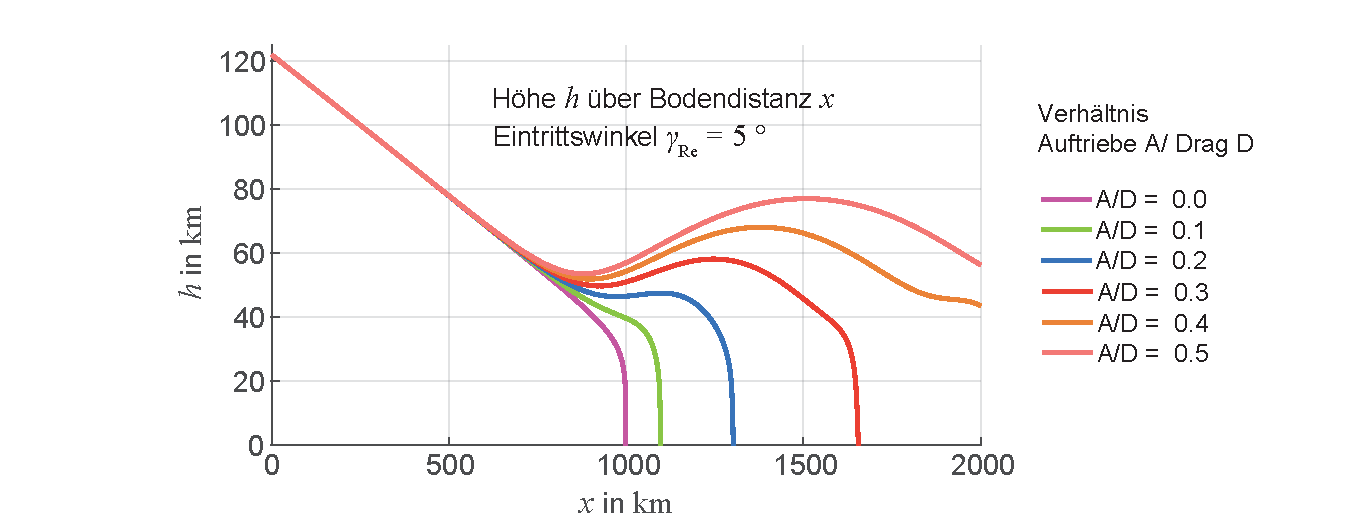
\includegraphics[width=\textwidth]{Reentry_Uebung01.pdf}
\caption[H�he $h$ nach Wiedereintritt in die Erdatmosph�re �ber die Bodendistanz $x$.]{H�he $h$ nach Wiedereintritt in die Erdatmosph�re �ber die Bodendistanz $x$ in Abh�ngigkeit vom Auftrieb/Drag-Verh�ltnis. Siehe \mscr~\mladynref{ReentryReal.m} f�r Parameter und Details.}
\label{abb:adyn_reentry_uebung01}
\end{figure}

\begin{figure}[H]
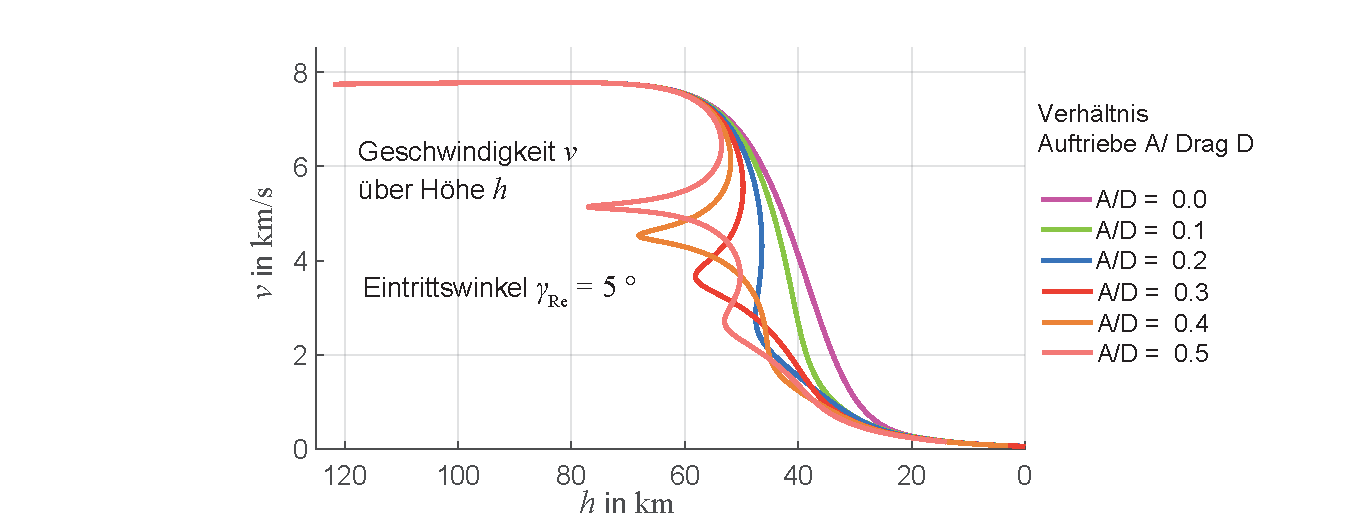
\includegraphics[width=\textwidth]{Reentry_Uebung02.pdf}
\caption[Geschwindigkeit $v$ nach Wiedereintritt in die Erdatmosph�re �ber die H�he $h$.]{Geschwindigkeit $v$ nach Wiedereintritt in die Erdatmosph�re �ber die H�he $h$ in Abh�ngigkeit vom Auftrieb/Drag-Verh�ltnis. Siehe \mscr~\mladynref{ReentryReal.m} f�r Parameter und Details.}
\label{abb:adyn_reentry_uebung02}
\end{figure}

\begin{figure}[H]
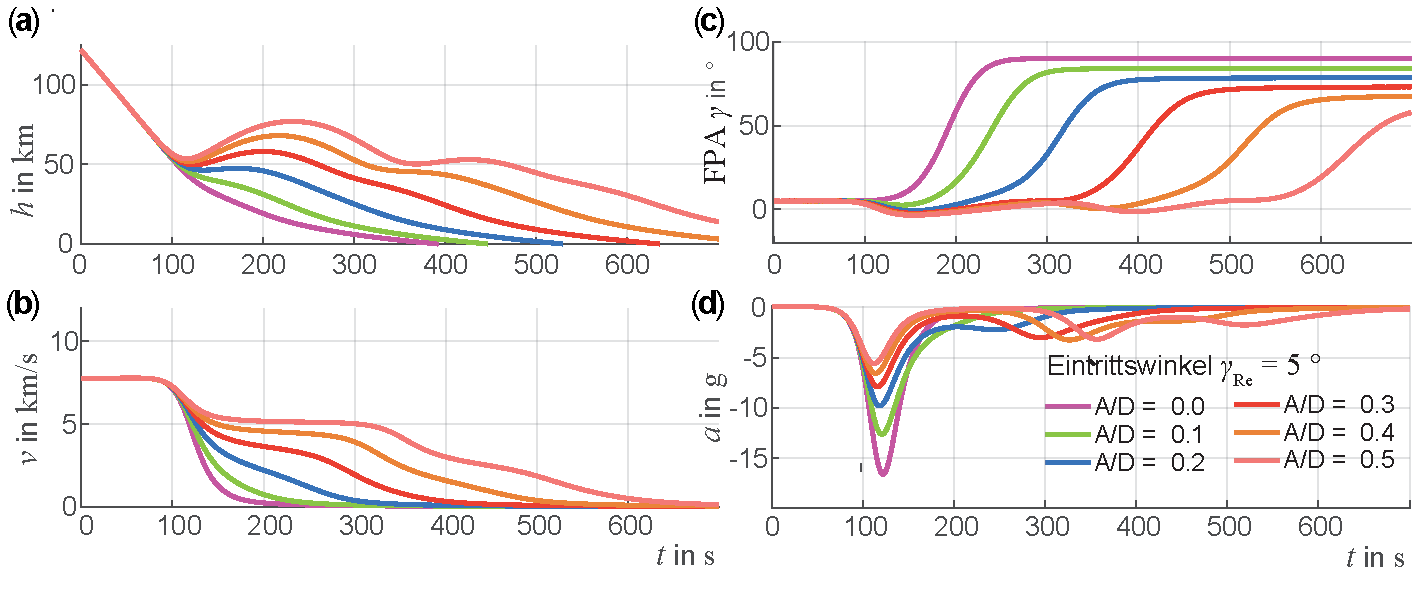
\includegraphics[width=\textwidth]{Reentry_Uebung03.pdf}
\caption[Verschieden Parameter nach Wiedereintritt als Funktion der Zeit.]{H�he $h$ \fa, Geschwindigkeit $v$ \fb, Flight Path Angle FPA \fc und Beschleunigung $a$ \fd nach Wiedereintritt in die Erdatmosph�re �ber die Zeit $t$ in Abh�ngigkeit vom Auftrieb/Drag-Verh�ltnis. Siehe \mscr~\mladynref{ReentryReal.m} f�r Parameter und Details.}
\label{abb:adyn_reentry_uebung03}
\end{figure}

\end{sol} 
\textcolor{blue} {$\rightarrow$ zur} \probref{adyn_reentry02}.\\
\noindent\rule[1ex]{\textwidth}{0.5pt}  \newpage  \clearpage

%-----------------------------------------------------------------------------------------------------------

\begin{sol}{prob:adyn_reentry03}\label{lsg:adyn_reentry03} %�bung29
\textbf{Normierte Gleichungen f�r $v(h)$ und $\gamma(h)$ bei Wiedereintritt}\\

F�r den Fall $F_\text{S}=0$ (was \zb f�r das Space Shuttle oft nicht erf�llt ist!) starten wir von:
\begin{subequations}
    \begin{align}
        \dot{v} &= -\frac{F_\text{D}}{m_\text{R}} - g\lk h\rk\,\sin\gamma = -v^2\,\frac{K_\text{D}}{H_0}\,\e^{-\frac{h}{H_0}}-g\,\sin \gamma\,,\\
        v\,\dot{\gamma} &= -\frac{F_\text{A}}{m_\text{R}} + \lk g\lk h\rk  - \frac{v^2}{r}\rk\,\cos\gamma\,,\\
        \dot{h} &= -v\,\sin\gamma\,,\\
        \dot{x} &= v\,\cos\gamma\,. 
    \end{align} \label{eq:adyn_normierte01}
\end{subequations}

Wir benutzen die barometrische H�henformel, sowie folgende Beziehungen f�r dem Drag und den Auftrieb:
\begin{subequations}
    \begin{align}
        F_\text{D} &= \frac{1}{2}\,\varrho\lk h\rk \,v^2\,C_\text{D}\,A_\text{R} = m_\text{R}\,v^2\,\frac{\kappa_\text{D}}{H_0}\,\e^{-\frac{h}{H_0}}\,,\\
        F_\text{A} &= \frac{1}{2}\,\varrho\lk h\rk \,v^2\,C_\text{A}\,A_\text{R} = m_\text{R}\,v^2\,\frac{\kappa_\text{A}}{H_0}\,\e^{-\frac{h}{H_0}}\,.
    \end{align} \label{eq:adyn_normierte02}
\end{subequations}

F�r $g\lk h\rk$ setzen wir an:
\begin{align}
    g\lk h\rk = g_0\,\frac{R_\text{E}{}^2}{r^2} = g_0\,\frac{R_\text{E}{}^2}{\lk R_\text{E}+h\rk^2}\,.  \label{eq:adyn_normierte03}
\end{align}
Wir normalisieren nun das DGL-System mit:
\begin{align}
    \begin{split}
        \mu &= \frac{v}{v_\text{K}} = \frac{v}{\sqrt{g_0\,R_\text{E}}} = \frac{v}{\sqrt{G\,M_\text{E}}}\\
        \eta &= \frac{h}{H_0}\,, ~~~~~~~~ \tau = \frac{g_0}{v_\text{K}}\,t\,, ~~~~~~~~
        \chi= \frac{x}{H_0}\, \\
        \D\tau &= \frac{g_0}{v_\text{K}}\,\D t\,, ~~~~~~~~ \D t = \frac{v_\text{K}}{g_0}\,\D \tau
    \end{split}\label{eq:adyn_normierte04}
\end{align}
und erhalten:
\begin{subequations}
    \begin{align}
        \begin{split}
            \frac{\D}{\D t}\,v &= -v^2\,\frac{\kappa_\text{D}}{H_0}\,\e^{-\frac{h}{H_0}} +g_0\,\frac{R_\text{E}{}^2}{r^2}\,\sin\gamma ~~~
            \rightarrow ~~~ \frac{\D}{\D \tau}\,\mu = -\mu^2\,\kappa_\text{D}\,\frac{R_\text{E}}{H_0}\,\e^{-\eta} +\sin\gamma\,.
          \end{split}
          \label{eq:adyn_normierte05a}
    \end{align}
und
    \begin{align}
        \begin{split}
            v\,\frac{\D}{\D t}\,\gamma &= -v^2\,\frac{\kappa_\text{A}}{H_0}\,\e^{-\frac{h}{H_0}} +\lk g-\frac{v^2}{r}\rk\,\cos\gamma~~~
            \rightarrow ~~~~ \mu\,\frac{\D}{\D\tau}\,\gamma =  -\mu^2\,\kappa_\text{D}\,\frac{A}{D}\,\frac{R_\text{E}}{H_0}\,\e^{-\eta} +\lk 1-\mu^2\rk\,\cos\gamma\,. 
          \end{split}
          \label{eq:adyn_normierte05b}
    \end{align}\label{eq:adyn_normierte05}
\end{subequations}
Die Gleichungen f�r H�he und Bodendistanz werden einfach zu:
\begin{subequations}
    \begin{align}
      \frac{\D}{\D\tau}\,\eta
      & = -\frac{R_\text{E}}{H_0}\, \mu\,\sin\gamma\,,
        \label{eq:adyn_normierte06a}\\
      \frac{\D}{\D\tau}\,\chi
      & = +\frac{R_\text{E}}{H_0}\,\mu\,\cos\gamma\,. \label{eq:adyn_normierte06b}
    \end{align} 
\end{subequations}

Wir setzen jetzt $\hat{\epsilon} = \mu^2$ und $\hat{\eta} = 2\,\frac{\kappa_\text{D}}{\sin\gamma_\text{Re}}\,\e^{-\eta}$ in \eqref{eq:adyn_normierte05} ein und erhalten mit der Substitution $\D \tau \rightarrow \D \hat{\eta} $ (siehe Nebenrechnung):
\begin{subequations}
  \begin{align}
    \frac{\D\lk \ln \hat{\epsilon}\rk}{\D \hat{\eta}}
    &= - \frac{\sin\gamma_\text{Re}}{\sin\gamma}
      + \frac{2H_0}{\hat{\epsilon}\,\hat{\eta}\,R_\text{E}}\,,
      \label{eq:adyn_normierte07a}\\
    \frac{\D\lk \cos\gamma\rk}{\D \hat{\eta}}
    &= \frac{\sin\gamma_\text{Re}}{2}\,\frac{A}{D}
      - \lk \frac{1}{\hat{\epsilon}}-1 \rk \,\frac{H_0\,\cos\gamma}
      {\hat{\eta}\,R_\text{E}}\,.
      \label{eq:adyn_normierte07b}
  \end{align}\label{eq:adyn_normierte07}
\end{subequations}

Die erste Gleichung ist eine Gleichung f�r die Entwicklung der (dimensionslosen) Energie $\hat{\epsilon}$ als Funktion der (dimensionslosen) H�he $\hat{\eta}$ und die zweite eine des FPA $\gamma$ ebenfalls als Funktion der H�he.

\begin{nebenrechnungNeu}  {  }

  Zun�chst nehmen wir uns \eqref{eq:adyn_normierte07a} vor.
  Wir beginnen mit der Ableitung und ber�cksichtigen die eingef�hrten
  Koordinatentransformationen, die eine mehrfache Verkettung enthalten,
  \begin{equation}
    \frac{\D\lk \ln \hat{\epsilon}(\tau(\eta(\hat{\eta})))\rk}{\D \hat{\eta}}
    = \frac{\D \eta}{\D \hat{\eta}} \frac{\D\lk \ln \hat{\epsilon}
      (\tau(\eta))\rk}{\D \eta}
    = \frac{\D \eta}{\D \hat{\eta}} \frac{\D \tau}{\D \eta}
    \frac{\D\lk \ln \hat{\epsilon}(\tau)\rk}{\D \tau} \; .
  \end{equation}
  Um die Ableitung berechnen zu k�nnen, ben�tigen wir also die Umkehrungen
  der Koordinatentransformation
  \begin{equation*}
    \hat{\eta} = 2\,\frac{\kappa_\text{D}}{\sin\gamma_\text{Re}}\,\e^{-\eta}
    \qquad \to \qquad \eta = -\ln\lk \frac{\sin\gamma_\text{Re}}
    {2\,\kappa_\text{D}}\, \hat{\eta} \rk
  \end{equation*}
  \begin{subequations}
    und daraus
    \begin{equation}
      \frac{\D \eta}{\D \hat{\eta}} = - \frac{\D}{\D \hat{\eta}} \ln\lk
      \frac{\sin\gamma_\text{Re}}{2\,\kappa_\text{D}}\, \hat{\eta} \rk
      = -\frac{1}{\hat{\eta}}
      \label{eq:adyn_normierte08a}
    \end{equation}
    Weiterhin kennen wir aus \eqref{eq:adyn_normierte06a} $\D\eta / \D \tau$
    und berechnen
    \begin{equation}
      \frac{\D \tau}{\D \eta} = \frac{1}{\D \eta/\D \tau} = - \frac{H_0}
      {R_\mathrm{E}}\frac{1}{\mu \sin\gamma} \; .
      \label{eq:adyn_normierte08b}
    \end{equation}
  \end{subequations}
  Schlie�lich ber�cksichtigen wir noch
  \begin{equation}
    \frac{\D\lk \ln \hat{\epsilon}(\tau)\rk}{\D \tau}
    = \frac{\D\lk \ln \mu(\tau)^2 \rk}{\D \tau}
    = 2 \frac{\D\lk \ln \mu(\tau) \rk}{\D \tau}
    = \frac{2}{\mu} \frac{\D \mu(\tau)}{\D \tau} \; .
    \label{eq:adyn_ablLnEpsilon}
  \end{equation}
  Wir fassen nun \eqref{eq:adyn_ablLnEpsilon} mit den Ableitungen
  \eqref{eq:adyn_normierte08a} und \eqref{eq:adyn_normierte08b} zusammen,
  \begin{equation}
     \frac{\D\lk \ln \hat{\epsilon}\rk}{\D \hat{\eta}} 
     = \frac{2}{\hat{\eta}\,\mu^2\, \sin\gamma} \frac{H_0}{R_\mathrm{E}}
     \frac{\D \mu(\tau)}{\D \tau} \; ,
  \end{equation}
  und erhalten durch das Einsetzen von \eqref{eq:adyn_normierte05a}
  \begin{multline}
     \frac{\D\lk \ln \hat{\epsilon}\rk}{\D \hat{\eta}}
     = \frac{2}{\hat{\eta}\,\mu^2\, \sin\gamma} \frac{H_0}{R_\mathrm{E}}
     \lk -\mu^2\,\kappa_\text{D}\, \frac{R_\text{E}}{H_0}\,\e^{-\eta}
     +\sin\gamma \rk
     = -\frac{1}{\hat{\eta}}\, \frac{\sin\gamma_\text{Re}}{\sin\gamma}\,
     \underbrace{\frac{2\,\kappa_\text{D}}{\sin\gamma_\text{Re}}\e^{-\eta}
     }_{\hat{\eta}} + \frac{H_0}{R_\mathrm{E}} \frac{1}{\hat{\eta}\,\mu^2} \\
     = -\frac{\sin\gamma_\text{Re}}{\sin\gamma}
     + \frac{H_0}{\hat{\epsilon}\,\hat{\eta} \,R_\text{E}} \; .
  \end{multline}

  Vollkommen analog berechnen wir
  \begin{equation}
    \frac{\D\lk \cos \gamma(\tau(\eta(\hat{\eta})))\rk}{\D \hat{\eta}}
    = \frac{\D \eta}{\D \hat{\eta}} \frac{\D\lk \cos \gamma(\tau(\eta))\rk}
    {\D \eta}
    = \frac{\D \eta}{\D \hat{\eta}} \frac{\D \tau}{\D \eta}
    \frac{\D\lk \cos \gamma(\tau)\rk}{\D \tau} 
    = - \frac{\D \eta}{\D \hat{\eta}} \, \frac{\D \tau}{\D \eta} \,
    \sin\gamma \, \frac{\D \gamma(\tau)}{\D \tau} \; ,
  \end{equation}
  wobei wir wieder die Ableitungen \eqref{eq:adyn_normierte08a} und
  \eqref{eq:adyn_normierte08b} einsetzen und \eqref{eq:adyn_normierte05b}
  verwenden,
  \begin{multline}
    \frac{\D\lk \cos \gamma \rk}{\D \hat{\eta}}
    = -\frac{1}{\hat{\eta}\,\mu^2} \frac{H_0}{R_\mathrm{E}}\,
    \lk -\mu^2\,\kappa_\text{D}\,\frac{A}{D}\, \frac{H_0}{R_\mathrm{E}} \,
    \frac{R_\text{E}}{H_0}\,\e^{-\eta} +\lk 1-\mu^2\rk\,\cos\gamma \rk \\
    = \frac{1}{\hat{\eta}} \, \frac{A}{D}\, \frac{\sin\gamma_\text{Re}}{2}\,
    \underbrace{\frac{2\,\kappa_\text{D}} {\sin\gamma_\text{Re}}\e^{-\eta}
    }_{\hat{\eta}}
    - \frac{H_0}{R_\mathrm{E}}\, \lk \frac{1}{\mu^2} - 1 \rk \frac{\cos\gamma}
    {\hat{\eta}} \\
    = \frac{\sin\gamma_\text{Re}}{2}\, \frac{A}{D}
    - \lk \frac{1}{\hat{\epsilon}} - 1 \rk \frac{H_0\,\cos\gamma}{\hat{\eta}\,
      R_\text{E}} \; .
  \end{multline}

\end{nebenrechnungNeu}

\end{sol} 
\textcolor{blue} {$\rightarrow$ zur} \probref{adyn_reentry03}.\\
\noindent\rule[1ex]{\textwidth}{0.5pt}  \newpage  \clearpage

%-----------------------------------------------------------------------------------------------------------

\begin{sol}{prob:adyn_reentry04}\label{lsg:adyn_reentry04} %�bung30
\textbf{ISS Stabilit�t - Absturz und Vergl�hen des Satelliten Tiangong-1}\\

\begin{figure}[H]
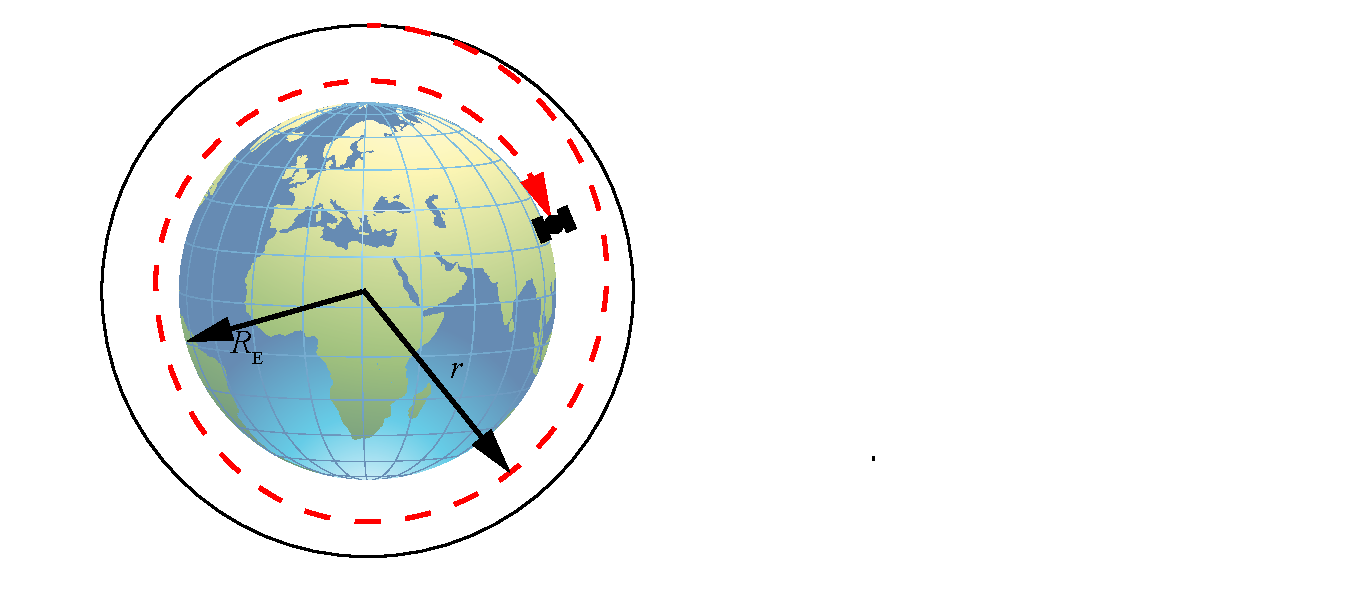
\includegraphics[width=\textwidth]{Tiangong01.pdf}
\caption[Einfaches Modell zur Berechnung des Absturzes des chinesischen Satelliten Tiangong-1.]{Einfaches Modell zur Berechnung des Absturzes des chinesischen Satelliten Tiangong-1.}
\label{abb:adyn_Tiangong01}
\end{figure}


\begin{enumerate}
\item [1.] Wir k�nnen aus \figref{adyn_ISS2004} folgende Raten des Radiusabfalls f�r das Jahr 2014 bestimmen: \\
    \begin{align*}
        \frac{\Delta a}{\Delta t} &= \SI{-1.578e-6}{\km\per\second} \pm \SI{1.0e-6}{\km\per\second} \approx \SI{-130}{\metre\per\day}\pm \SI{80}{\metre\per\day}
    \end{align*}
    Daraus erh�lt man �ber \eqref{eq:adyn_tiangong03} und \eqref{eq:adyn_tiangong05} eine effektive Fl�che 
    \begin{align*}
        A_\text{eff} = \kappa_\text{D}\,A_\perp \approx \SI{210}{\square\metre} \pm \SI{140}{\square\metre}\,,
    \end{align*}
    was eher am unteren Ende der Erwartung liegt, wenn man
    \begin{align*}
        A_\perp \approx
        \begin{cases}
            \SI{50}{\metre}\cdot\SI{70}{\metre} = \SI{3500}{\square\metre}\\
            \SI{109}{\metre}\cdot\SI{51}{\metre} \approx \SI{5000}{\square\metre}
        \end{cases}
    \end{align*}
    entsprechend der Literatur ansetzt, wobei man hierbei das Sonnensegel als voll ausgebreitet in Flugrichtung annimmt. Wir m�ssten dann von einem relativ niedrigen $\kappa_\text{D}$ Wert von $\SI{0.1}{}$ ausgehen. \\
    Fehler in unserer Absch�tzung k�nnen vor allem in der Dichteberechnung liegen. Eine �berpr�fung mit dem Harries-Priester-Modell \cite{Montenbruck2012} ergibt f�r eine H�he von $\SI{420}{\km}$ Werte von $\varrho$ zwischen $\SI{1.558}{\g\per\cubic\km}$ und $\SI{5.684}{\g\per\cubic\km}$ je nach Tageszeit eine etwas bessere �bereinstimmung mit den $A_\text{eff}$-Werten aus der Literatur!\\
    Im Fall eines Magnetsturms kann man von einer Zunahme der Partikeldichte ausgehen, die wegen
    \begin{align*}
        \frac{\Delta a_1/\Delta t}{\Delta a_0/\Delta t} = 4 = \frac{\varrho_1}{\varrho_0}
    \end{align*}
    in etwa proportional zur Zunahme der Rate des Radiusabfalls ist. \\
\item [2.] Wir k�nnten zur Berechnung nat�rlich das Instrumentarium aus \kap{adyn_reentry} benutzen und da insbesondere die Gleichungen \eqref{eq:adyn_reentry02} \bzw \eqref{eq:adyn_reentry02}. Da uns aber wesentliche Informationen fehlen \bzw nicht in ausreichender Genauigkeit vorliegen, wollen wir ein einfaches Modell verwenden. Wir gehen von einer kreisf�rmigen Bahn aus, nehmen an, dass der Drag immer entgegengesetzt zur Richtung der Geschwindigkeit wirkt. Ebenso wird ein konstanter FPA von $\gamma=0$ angenommen. Damit k�nnen wir auch annehmen, dass die Verringerung der Energie des Satelliten (\figref{adyn_Tiangong01}) allein aus der Reibungsarbeit des Drags resultiert, also
    \begin{align}
        \frac{\D}{\D t} H = \frac{\D}{\D t}\lk \frac{\mu_\text{E}\,m_\text{R}}{2r}\rk = F_\text{D}\,v_\text{R}~~~\text{mit}~~~
        F_\text{D} = \frac{1}{2}\,\varrho\lk r\rk \,\kappa_\text{D}\,A_\perp\,v_\text{R}{}^2\,,\label{eq:adyn_tiangong01}
    \end{align}
    worin $\varrho\lk r\rk$ die Dichte der Restatmosph�re im Abstand $r$ vom Erdmittelpunkt und $A_\perp$ die wirksame Fl�che des Raumschiffs senkrecht zur Bewegungsrichtung ist, $\kappa_\text{D}$ ist der Drag-Koeffizient. \\
    Wir erhalten aus \eqref{eq:adyn_tiangong01} die einfache Differentialgleichung 
    \begin{align}
        \begin{split}
            \dot{r} &= -\kappa_\text{eff}\,\sqrt{r}\,\varrho\lk r\rk ~~~~ \text{\bzw mit} ~~~~ r = h + R_\text{E}\, \\
            \dot{h} &= -\kappa_\text{eff}\,\sqrt{h+R_\text{E}}\,\varrho\lk h\rk ~~~~ \text{und}~~~\kappa_\text{eff} = \sqrt{\mu_\text{E}}\,\frac{\kappa_\text{D}\,A_\perp}{m_\text{R}}\,.
        \end{split} \label{eq:adyn_tiangong03}
    \end{align}
    F�r $\varrho\lk h\rk$ benutzen wir ein Modell der Australian Space Weather Agency \cite{Fiolhais2023}:
    \begin{align}
        \varrho\lk h\rk = \SI{6e-1}{} \exp\lk-\frac{\lk h-h_0\rk}{H}\rk\,\SI{}{\kg\per\cubic\km}\label{eq:adyn_tiangong04}
    \end{align}
    mit $H= 29.5 \pm 0.1$ und h=\SI{175}{ \km}.\\
    Da $m_\text{R} = \SI{8.5e3}{\kg}$ bekannt ist, ist der einzig anzupassende Parameter in unserem Modell dann die effektive Fl�che $A_\text{eff} = \kappa_\text{D}\,A_\perp$:
    \begin{align}
        \kappa_\text{eff} = \sqrt{\mu_\text{E}}\,\frac{A_\text{eff}}{m_\text{R}} = \sqrt{\mu_\text{E}}\,\frac{\kappa_\text{D}\,A_\perp}{m_\text{R}}\,. \label{eq:adyn_tiangong05}
    \end{align}
    Wenn wir mit den Anfangswerten f�r Apog�um und Perig�um von $\SI{286}{\km}$ \bzw $\SI{274}{\km}$ eine Anpassung an die experimentellen Werte vornehmen, erhalten wir $A_\text{eff,A} \approx \SI{63}{\square\metre}$ \bzw $A_\text{eff,P} \approx \SI{33}{\square\metre}$, was mit den Abmessungen der Raumstation von $\SI{4}{\metre}\cdot\SI{10}{\metre}$ relativ gut �bereinstimmt (\figref{adyn_Tiangong02}). Gleichwohl ist der Unterschied zwischen den Perig�ums- und Apog�umswerten recht gro�, was aber an unserem einfachen Modell liegt. \\
    Der Leser �berlege sich, ein verbessertes (numerisches) Modell, welches die Elliptizit�t der Anfangsbahn ber�cksichtigt und den Drag dann st�ckweise auf der elliptischen Bahn ber�cksichtigt. Welche weiteren Verbesserungen des Modells sind dar�ber hinaus denkbar und relativ einfach umzusetzen?\\

\begin{figure}[H]
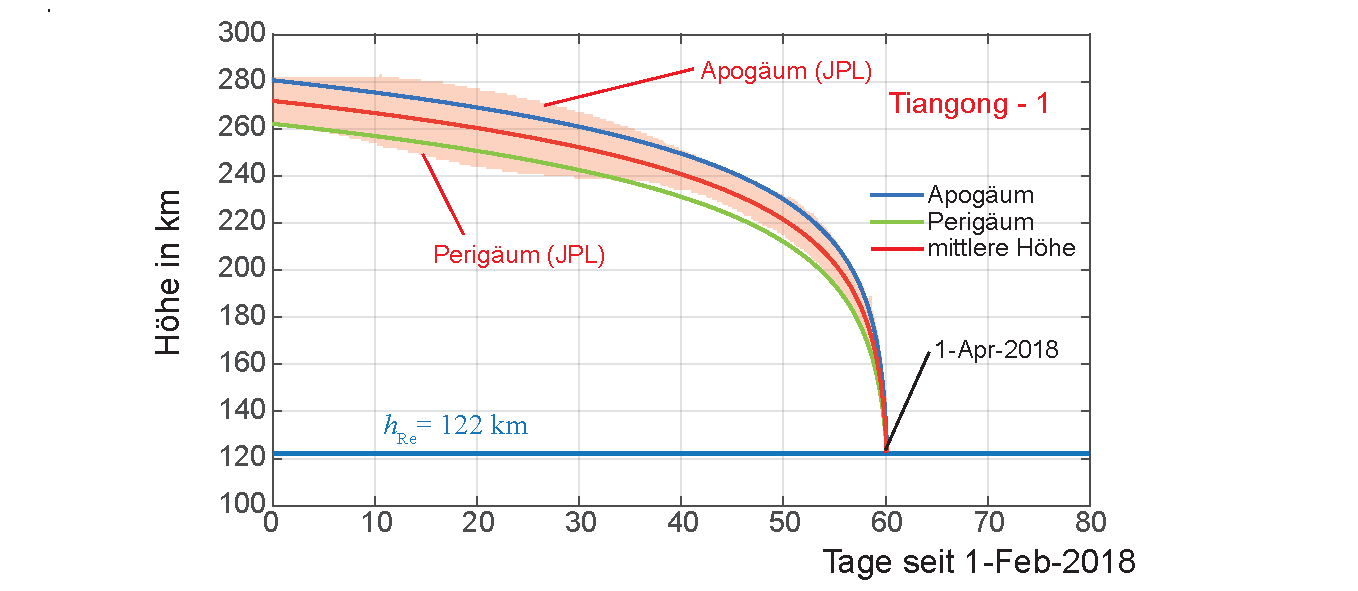
\includegraphics[width=\textwidth]{Tiangong02.pdf}
\caption[Zeitliche Entwicklung des Bahnradius bis zum Absturz des chinesischen Satelliten Tiangong-1.]{Zeitliche Entwicklung des Bahnradius des chinesischen Satelliten Tiangong-1.}
\label{abb:adyn_Tiangong02}
\end{figure}

\end{enumerate}    

Alle Rechnungen sind im \mscr~\mladynref{OrbitalDecay.m} hinterlegt. 

\end{sol} 
\textcolor{blue} {$\rightarrow$ zur} \probref{adyn_reentry04}.\\
\noindent\rule[1ex]{\textwidth}{0.5pt}  \newpage  \clearpage

%-----------------------------------------------------------------------------------------------------------

\begin{sol}{prob:adyn_BoatRocketModel}\label{lsg:adyn_BoatRocketModel} %�bung31
\textbf{Zur Entspannung}\\

Die anf�ngliche Gesamtmasse $M$ besteht aus der Boot- und K�rpermasse $m_\text{B},\, m_\text{L}$, sowie den $N$ Kokosn�ssen mit der Masse $m_\text{K}$ pro Nuss.
    \begin{align}
        M &= m_\text{L} + m_\text{B} + \sum\limits_1^N m_\text{K} \,. \label{eq:adyn_RaketenAlt01}
    \end{align}
F�r jeden Abwurf einer Kokosnuss schreiben wir sukzessive die Geschwindigkeit $V_i$ des Bootes nach Abwurf einer Kokosnuss �ber die Impulserhaltung auf:\\
\underline{1. Abwurf:} 
    \begin{align}
        -m_\text{K}\,v_\text{K} + \lk M-m_\text{K}\rk \,V_1 &= 0 ~~~~
        \rightarrow  ~~~~~ V_1 &= \frac{m_\text{K}}{M-m_\text{K}}\,v_\text{K}\label{eq:adyn_RaketenAlt02}
    \end{align}\\
\underline{2. Abwurf:} 
    \begin{align}
        -m_\text{K}\,\lk v_\text{K} - v_1\rk + \lk M-2m_\text{K}\rk\,V_2 &= \lk M-m_\text{K}\rk\,V_1 ~~~~
        \rightarrow ~~~~ V_2 &= \lek \frac{m_\text{K}}{M-m_\text{K}} + \frac{m_\text{K}}{M-2m_\text{K}}\rek\,v_\text{K} \label{eq:adyn_RaketenAlt03}  
    \end{align}\\
\underline{N-te Abwurf} 
    \begin{align}
        V_N = \sum\limits_{n=1}^N \frac{m_\text{K}\,v_\text{K}}{M-n\,m_\text{K}} = \frac{m_\text{K}\,v_\text{K}}{M}\,\sum\limits_{n=1}^N\,\frac{1}{1-n\,\frac{m_\text{K}}{M}}\label{eq:adyn_RaketenAlt04}  
    \end{align}

Man kann leicht mit \matlab{} zeigen, dass diese Summe konvergiert. Man beachte dabei, dass $N\,m_\text{K} = M-m_\text{L} - m_\text{B}$ ist. \\
F�hren wir die Masse $m_\text{G} = n\,m_\text{K}$ als die Masse der geworfenen Kokosn�sse ein, 
\begin{align}
    V_n &= v_\text{K}\,\sum\limits_{n=1}^N\,\frac{1}{\mu^N-n} ~~~~ \text{mit} ~~~~ \mu = \frac{n\,M_0}{M_\text{T}} = \frac{n\,M_0}{n\,m_\text{K}} ~~~~ \rightarrow ~~~~ \mu = \frac{M_0}{m_\text{K}}>1 \nonumber \\
    &= v_\text{K}\,\lek \frac{1}{\mu-1}+\frac{1}{\mu-2} + \ldots +\frac{1}{\mu-n}\rek \label{eq:adyn_RaketenAlt05}  
\end{align}
Wir bilden nun den Grenzwert:
\begin{align}
    \lim_{N\to\infty} V_N = v_\text{K}\, \lim_{N\to\infty}\sum\limits_{n=1}^N\,\frac{1}{\mu-n}\label{eq:adyn_RaketenAlt06}\,.
\end{align}
Im \mscr ~ \mladynref{AlternativRaketenGL.m} l�sst sich die Grenzwertbildung gut numerisch simmulieren. Das Ergebnis ist in \figref{adyn_RaketenAlternative} gezeigt.\\
Wir ersetzen $\mu = n\,M_0/M_\text{T} = n/x$ mit $0<x=M_\text{T}/M_0<1$:
\begin{align}
    V_N = v_\text{K}\sum\limits_{n=1}^N\,\frac{1}{n/x-n}\,\frac{x}{x} = v_\text{K}\sum\limits_{n=1}^N\,\frac{x}{n-n\,x}\label{eq:adyn_RaketenAlt07}\,.
\end{align}

\begin{figure}[H]
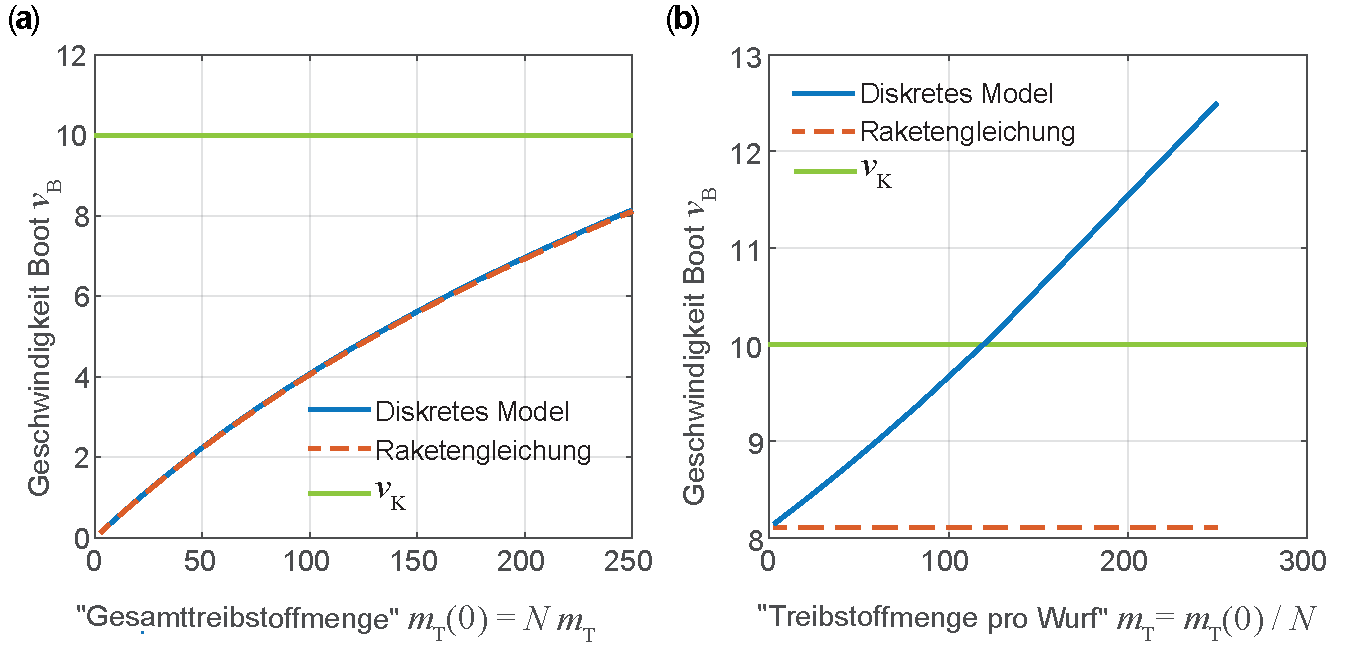
\includegraphics[width=\textwidth]{BoatRocketModelLsg.pdf}
\caption[Diskretes Modell der Raketengleichung.]{Diskretes Modell der Raketengleichung.}
\label{abb:adyn_RaketenAlternative}
\end{figure}


\begin{nebenrechnungNeu} {Grenzwertberechnung}
  
Wir wollen den Grenzwert bilden:
\begin{align}
    \lim_{N\to\infty} V_N &= v_\text{K} \lim_{N\to\infty} \lk \frac{1}{\mu-1} + \frac{1}{\mu-2} + \ldots + \frac{1}{\mu-n}\rk \nonumber \\
    &= v_\text{K} \lim_{N\to\infty} \lk \frac{x}{n-x} + \frac{x}{n-2x} + \ldots + \frac{n}{n-n\,x} \rk = S(x) \label{eq:adyn_RaketenAlt08}
\end{align}
Wir berechnen zun�chst die Partialsumme $S_k^n$, die die Summe aller Terme der Summe $V_n$ nach \eqref{eq:adyn_RaketenAlt08} bis zum $k$-ten Term beinhaltet. Wir definieren dies wie folgt rekursiv:
\begin{align}
    S_{k+1}^n = S_{k}^n + \frac{x}{n-\lk k+1\rk\,x} ~~~~ \text{mit} ~~~~ n=1,2,\ldots,N ~~~~\text{und} ~~~~ k = 0,1,\ldots,\lk n-1\rk\label{eq:adyn_RaketenAlt09}
\end{align}
Dabei ist:
\begin{align*}
    S_0^1 = 0
    \begin{cases}
        n=1,\, k=0
    \end{cases}
    ~~~\text{und}~~~
    S_1^1 = S_0^1 + \frac{x}{1-x} = \frac{x}{1-x}
    \begin{cases}
        n=1,\, k=1
    \end{cases}
\end{align*}
Wir bilden den Quotienten:
\begin{align}
    \frac{S_{k+1}^n - S_k^n}{x/n} = \frac{1}{1-\lk k+1\rk \,x/n}\label{eq:adyn_RaketenAlt10}
\end{align}
und bezeichnen der Einfachheit wegen: 
\begin{align}
    \lk k+1\rk\,\frac{x}{n} = \chi_\text{k} \label{eq:adyn_RaketenAlt11}
\end{align}
und 
\begin{align}
    S_{k+1}^n - S_k^n = \Delta S\lk \chi_\text{k}\rk\,.  \label{eq:adyn_RaketenAlt12}
\end{align}
Damit wird aus \eqref{eq:adyn_RaketenAlt10} der Differentialquotient
\begin{align}
    \frac{\Delta S\lk \chi_\text{k}\rk}{\Delta \chi_\text{k}} = \frac{1}{1-\chi_\text{k}}\,. \label{eq:adyn_RaketenAlt13}
\end{align}
Wir bilden den Grenzwert $n\to\infty$ und erhalten mit $S\lk \chi_\text{k}\rk$ das Riemann-Integral der rechten Seite:
\begin{align}
    S\lk \chi_\text{k}\rk = -\ln\lk 1-\chi_\text{k}\rk = \ln \lk \frac{1}{1-\chi_\text{k}}\rk\,. \label{eq:adyn_RaketenAlt14}
\end{align}
Mit \eqref{eq:adyn_RaketenAlt11} k�nnen wir f�r $n\to\infty$ auch schreiben ($k=n,\,\chi_\text{k}\to x$)
\begin{align*}
    S\lk \chi_\text{k}\rk = S\lk x\rk
\end{align*}
also:
\begin{align}
    \ln\lk \frac{1}{1-x}\rk = \lim_{n\to\infty} \lk \frac{x}{n-x} + \frac{x}{n-2x} +\ldots + \frac{x}{n-n\,x}\rk\,. \label{eq:adyn_RaketenAlt15}
\end{align}
Damit wird aus \eqref{eq:adyn_RaketenAlt11}
\begin{align}
    V= \lim_{n\to\infty} V_N = v_\text{k}\,\ln\lk\frac{1}{1-x}\rk = v_\text{k}\,\ln\lk\frac{1}{1-M_\text{T}/M_0}\rk = v_\text{k} \,\ln\frac{M_0}{M_0-M_\text{T}}\,, \label{eq:adyn_RaketenAlt16}
\end{align}
was genau der Raketengleichung \eqref{eq:adyn_rocketequ} entspricht. (Diese Rechnung wurde in �hnlicher Form zuerst in \cite{Lagos2023} gezeigt.)\\

\end{nebenrechnungNeu}


\end{sol} 
\textcolor{blue} {$\rightarrow$ zur} \probref{adyn_BoatRocketModel}.\\
\noindent\rule[1ex]{\textwidth}{0.5pt}  \newpage  \clearpage

%-----------------------------------------------------------------------------------------------------------
%-----------------------------------------------------------------------------------------------------------

\newpage
\subsection{Weiterf�hrende Zusatzaufgaben und Probleme}

\begin{sol}{prob:adyn_launchinnovations}\label{lsg:adyn_launchinnovations} %Zusatz1
\textbf{Neue Ideen zum Flug ins Weltall}\\

Wir zitieren aus der etwas sp�rlichen Information der Firma Spinlaunch (\url{www.spinlaunch.com}):
\begin{quotation}
\textit{The Suborbital Accelerator is designed to operate from 800 to 5,000 mph (approx. 8000 km/h) and acts primarily as a test-bed for the Orbital Launch System. On October 22nd, 2021, our first launch successfully propelled a test vehicle at supersonic speeds and ended with the recovery of the reusable flight vehicle. Throughout 2022 the system will conduct regular test flights with a variety of vehicles and launch velocities. The Suborbital System offers testing capabilities to customers and provides long term value as a satellite qualification facility.
}
\end{quotation}
So weit so gut. Schauen wir uns diese neueren Ideen f�r den Weltraumflug genauer an:\\
Den Weltraumfahrstuhl haben wir bereits in �bung 1.10 von Band I untersucht und verweisen daher auf die entsprechende L�sung.\\
Die \anf{Weltraumachterbahn}, wie der Spinlaunch auch genannt wird, ist ein neues Konzept und wir wollen uns die Machbarkeit unter drei Gesichtspunkten genauer anschauen. Wir benutzen dabei Angaben, die von der Fa. SpinLaunch \bzw in der Literatur im Internet zu finden sind.\\
Danach soll der Raumtransporter (Anfangsmasse von $m_0 = \SI{250}{\kg}$) die Zentrifuge mit einer Geschwindigkeit von $\SI{1000}{}$ - $\SI{8000}{\km\per\hour}$ verlassen und ohne Antrieb eine H�he von $\SI{60}{\km}$ �ber der Erdoberfl�che erreichen, wo eventuell noch einmal mit einer mitgenommenen Treibstoffmenge von $\SI{100}{\kg} \ldots \SI{150}{\kg}$
eine weitere Beschleunigung erfolgen kann. 
Der Durchmesser der Zentrifuge betr�gt etwa  $D=2R=\SI{50}{\metre}$.\\
Wir wollen untersuchen:
\begin{itemize}
    \item [1)] 
    \textbf{\textit{Mechanische Herausforderungen an die Zentrifuge}}:\\
    Es gilt: $v_0 = \omega\,D \quad \rightarrow \quad \omega = v_0/D$.\\
    Mit den geforderten Werten erhalten wir $\omega \approx 120,\ldots,1000\,\SI{}{\per\second}$.\\
    Wir gehen davon aus, dass das Raumschiff durch ein Gest�nge in der Zentrifuge geleitet wird. Das Gest�nge soll einen effektiven Durchmesser von $D = \SI{0.5}{\metre}$ haben und aus Stahl \bzw Kohlenfaserverbundstoffen bestehen.\\
    Die gesamte Zugspannung auf das Gest�nge  betr�gt dann:
    \begin{align*}
        \sigma = A\,\varrho\,\frac{R^2}{2}\,\omega^2 + m_0\,\omega^2\,\frac{R}{A} 
    \end{align*}
mit $A=\pi D^2/4$  und $\varrho \approx \SI{7e3}{\kg\per\cubic\metre}\,\text{(Stahl)}\, \text{\bzw}\, \varrho = \SI{2e3}{\kg\per\metre}\,\text{(Kohlenfaser)}$.  Wir erhalten\\
$\sigma = \SI{6.6}{\giga\Pa}$ (Stahl) \bzw $\sigma= \SI{2.2}{\giga\Pa}$ (Kohlenfaser).\\
Diese Werte sind dicht an der maximal erreichbaren Zugspannung vor einer m�glichen Zerst�rung. Hierin liegt also eine erste Herausforderung in der Lagerung des Zentrifugalarms, diese enormen Radialkraft muss ja durch das Lager aufgenommen werden.\\
    \item [2)]
    \textbf{\textit{Antriebsloser Aufstieg}}:\\
Nach Ausl�sen aus der Zentrifuge tritt der  Raumtransporter aus dem Vakuum in die Erdatmosph�re und erf�hrt auf dem Weg nach oben neben den gravitativen Verlusten auch Reibungsverluste.\\
    Wir k�nnen die Ergebnisse von \probref{adyn_launch01} benutzen und erhalten unter der Annahme von optimistischen Werten von $c_\text{w,R} = 0.2$ und $A_\text{R} = \pi\,\SI{0.25}{\square\metre}/4$ eine maximale H�he am Ende der Spin Launch Phase von $h_\text{end} = \SI{50}{\km},\ldots,\SI{60}{\km}$ \bzw eine Geschwindigkeit von $v_\text{end}\lk h=\SI{60}{\km}\rk\approx \SI{1.25}{\km\per\second}$.\\
    \item [3)]
    \textbf{\textit{Zusatzschub}}:\\
    Nimmt man an, dass bei $h=\SI{60}{km}$ noch $\SI{200}{\kg}$ Treibstoff mit $v_\text{G}=\SI{5000}{\metre\per\second}$ (sehr optimistisch) zur Verf�gung stehen, dann hat man dort f�r die verbleibende Nutzlast von $\SI{100}{kg}$ (ohne Strukturmasse) noch ein Geschwindigkeitsbudget von
    \begin{align*}
        \Delta v = v_\text{G}\,\ln\,\frac{m_\text{L}}{m_0}\, = \SI{5.9}{\km\per\second}
    \end{align*}
    zur Verf�gung, zus�tzlich der 
    \begin{align*}
        \Delta v_\text{E} \approx \SI{0.4}{\km\per\second}
    \end{align*}
    aus der Rotation der Erde.\\
    Gebraucht werden f�r eine Kreisbahn in $\SI{200}{\km}$:
    \begin{align*}
        v_\text{k} =  \sqrt{ \frac{\mu_\text{E}}{R_\text{E}}+\SI{200}{\km}}\approx \SI{7.85}{\km\per\second}\,,
    \end{align*}
    \dh unter den Annahmen kommt es zu keiner stabilen Kreisbahn in $\SI{200}{\km}$ H�he, es wird sich also um einen suborbitalen Flug handeln.\\
		\item [4)] 
    Wir wollen nun noch die energetischen Verh�ltnisse betrachten.\\
    Um eine Nutzlast von $\SI{100}{\kg}$ mit in eine H�he von $\SI{200}{\km}$ zu bringen, braucht man (ohne Ber�cksichtigung der Unterst�tzung durch die Erdrotation) ein Geschwindigkeitsbudget von 
    \begin{align*}
        \Delta v = \SI{7.85}{\km\per\second}
    \end{align*}
    \bzw bei Annahme einer Strukturmasse von $\SI{500}{\kg}$ eine Treibstoffmasse von 
    \begin{align*}
        m_\text{T} = m_\text{L} \, \lk \e^{+\frac{\Delta v}{v_\text{G}}} - 1 \rk - m_\text{S} \approx \SI{300}{\kg}\,.
    \end{align*}
    Man spart also in etwa $\SI{100}{\kg}$ Treibstoff. Daf�r muss man durch elektrischen Antrieb eine kinetische und Rotationsenergie von 
    \begin{align*}
        T = \frac{m_0}{2}\,v_0{}^2 + \frac{J}{2}\,\lk\frac{v_0}{R}\rk^2 = \frac{1}{2}\,v_0{}^2\,\lk m_0 + \frac{J}{R^2} \rk
    \end{align*}
    aufbringen, wenn $J$ das Tr�gheitsmoment des Rotationsarms ist.
    \begin{align*}
        J &= \frac{1}{3}\,m_{\text{Rotor}}\,R^2 = \frac{1}{3}\,\frac{\pi}{4}\,D^2\,R^3 \,\varrho \approx \SI{1.8}{\kg\square\metre}\\
        \rightarrow \quad T & \approx \SI{5.8}{\N\metre} \approx \SI{1.6}{\mega\watt\hour}
    \end{align*}
    Der \anf{eingesparte} Treibstoff (typische Parameter) hat einen \anf{Energieinhalt} von
    \begin{align*}
        E_{\text{chem}} &= \epsilon_\text{T}\,\Delta m_\text{T}\\
        &\approx \SI{3500}{\kilo\joule\per\mol}\cdot\SI{0.01}{\mol\per\g}\cdot\SI{100e3}{\g} \approx \SI{3.5e9}{\joule} \approx \SI{1}{\mega\watt\hour}
    \end{align*}
    Auch daran sieht man, dass man energetisch nicht wirklich etwas spart (wie k�nnte man auch?), jedoch w�re der Betrieb der SpinLaunch-Anlage nat�rlich mit \anf{nachhaltiger} Energie machbar.\\
    \item [5)]
    \textbf{\textit{Zusammenfassung}}:\\
    Alles in allem sieht das Projekt SpinLaunch etwas erfolgversprechender aus als der Erdfahrstuhl, wenngleich die ingenieurtechnischen Anforderungen riesig sind und auch der f�r 2022 angek�ndigte Erstflug bislang nicht erfolgt ist. \\
    In \figref{adyn_SpinLaunch} haben wir das Ergebnis der Simulation eines SpinLaunch-Unternehmens f�r eine Nutzlast von \SI{100}{\kg} und einem \textit{on-board} Treibstoffvorrat von $\SI{200}{\kg}$ dargestellt. Auch sonst sind alle anderen Annahmen extrem optimistisch gemacht. Man erkennt, dass dieses Prinzip bestenfalls f�r kleinere Nutzlasten machbar/sinnvoll erscheint, wobei wir mal von den \anf{kleinen} ingenieurtechnischen Herausforderungen wie Vakuum f�r die Zentrifuge, Stabilit�t der Materialien, Bewegung von $\SI{200}{\kg}$ Treibstoff bei einer \anf{leicht erh�hten} Zentrifugalbeschleunigung von $a_\text{z} = v_0{}^2/R\approx \SI{20e3}{} g$ absieht.
\end{itemize}


\begin{figure}
	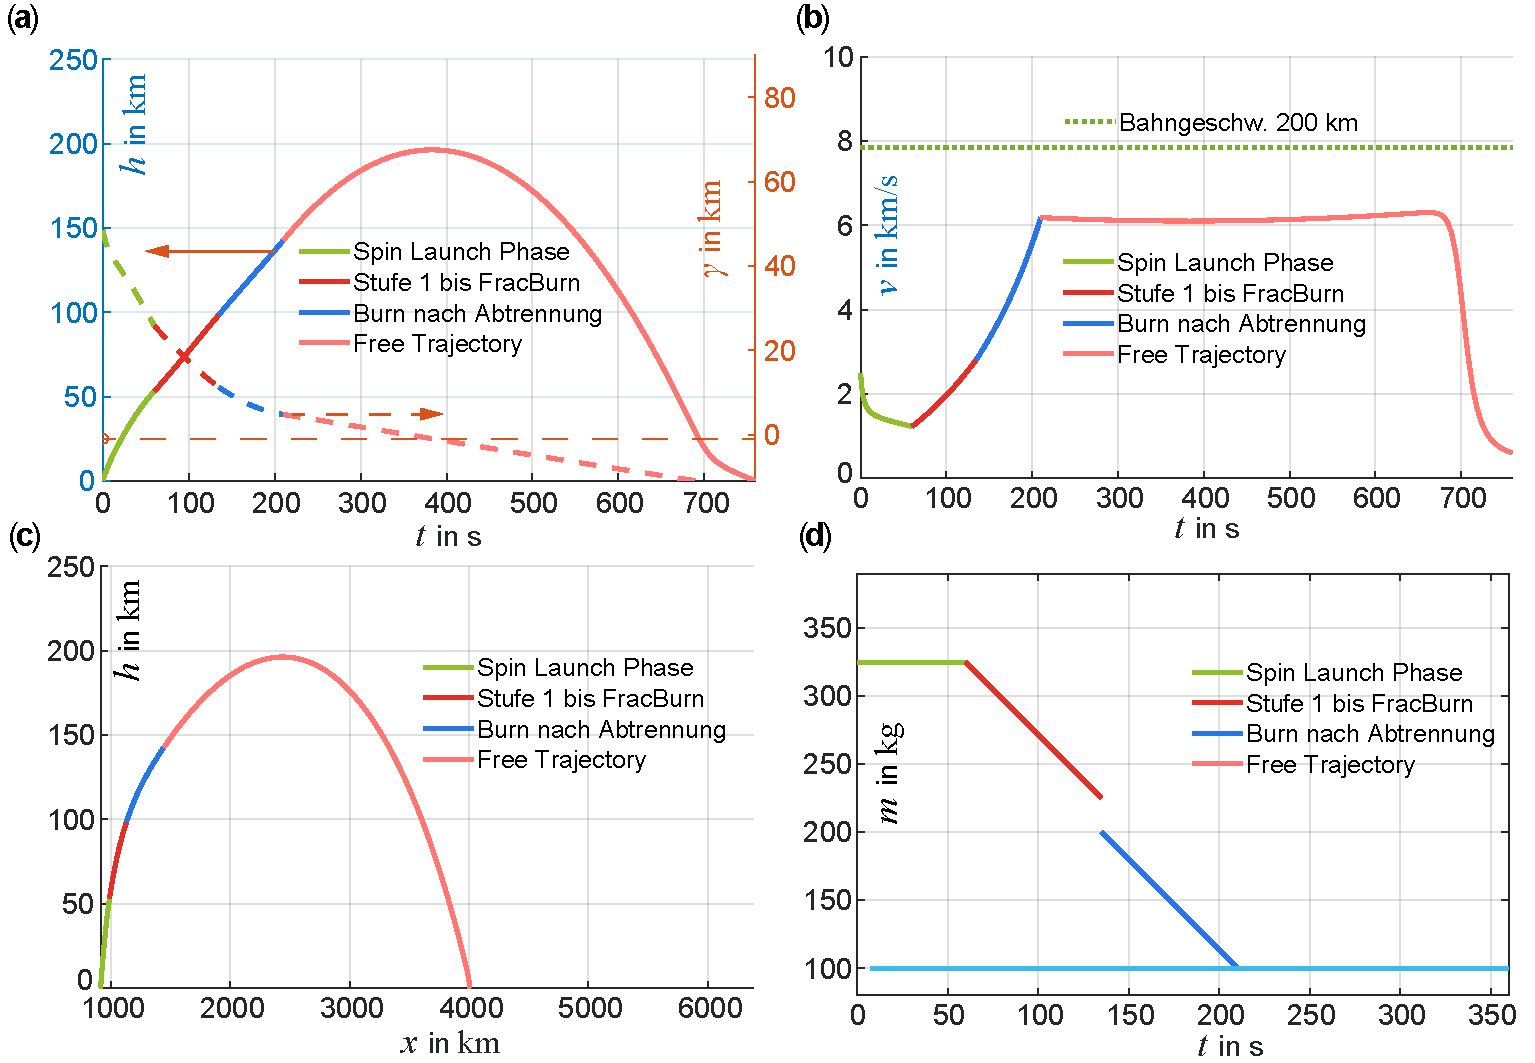
\includegraphics[width=\textwidth]{Spinlaunch.pdf} 
	\caption[Beispielrechnungen zum Spinlaunch.]{Beispielrechnungen zum Spinlaunch. Parameter siehe Text und \mscr~\mladynref{Spinlaunch.m} \fa H�he und FPA �ber die Zeit \fb Geschwindigkeit �ber die Zeit \fc H�he �ber Horizontkoordinate $x$ \fd Masse des Raumtransporters �ber die Zeit.}
	\label{abb:adyn_SpinLaunch}
\end{figure}

\end{sol} 
\textcolor{blue} {$\rightarrow$ zur} \probref{adyn_launchinnovations}.\\
\noindent\rule[1ex]{\textwidth}{0.5pt} \newpage  \clearpage


%-----------------------------------------------------------------------------------------------------------

\begin{sol}{prob:adyn_orbits_zusatz2}\label{lsg:adyn_orbits_zusatz1} %Zusatz
\textbf{Bahnparameter aus Bodenbeobachtungen (Ortsvektoren)}\\

Zun�chst m�ssen wir aus den topozentrischen Messwerten ($\vec{R}$ mit Distanz $R$, Azimut $\mathcal{A}$ und H�he $h$) geozentrisch-�quatoriale Messwerte "`machen"'. Wir invertieren dazu \eqref{eq:adyn_statobserv06} und erhalten:
\begin{align}
	  \vec{r} =  \mathbb{R}_\text{z}\lk -\theta\rk \, \lek \mathbb{U}^{-1} \,\vec{R} + \vec{r}_\text{B} \rek \,, \label{eq:adyn_bahnbest_lsg01}
\end{align}
worin $\vec{r},\, \vec{r}_\text{B}$ die geozentrische-�quatorialen Koordinatenvektoren f�r Satellit und Beobachtungsstation sind und  $\vec{R}$ die topozentrischen Koordinaten des Satelliten.\\
Mit den so bestimmten Vektoren $\vec{r}_1$ und $\vec{r}_2$ zu den beiden Messzeiten /$t_1,$ und $t_2$ kann man nach einer von Gau� entwickelten geometrisch-iterativen Methode die Bahnparameter bestimmen. Im folgenden ist diese der Darstellung in \cite{Montenbruck2012} folgend skizziert. Wir starten mit \figref{adyn_orbit_determination} und gehen wie folgt vor:

\begin{figure}
	\includegraphics[width=\textwidth]{BestimmungOrbitsGauss.pdf} 
	\caption[Bestimmung von Bahnparametern von Satelliten.]{Zur Bestimmung von Bahnparametern von Satelliten aus Orts- und Winkelbeobachtungen.}
	\label{abb:adyn_orbit_determination}
\end{figure}

\begin{enumerate}
    %1
    \item Man benutzt, dass die Bahnebene eines Satelliten immer durch die Ebene gegeben ist, die durch die beiden Vektoren $\vec{r}_1$, $\vec{r}_2$ aufgespannt wird. \\
    Man bestimmt dann �ber die Einheitsvektoren 
    \begin{align}
        \vec{e}_1 &= \frac{\vec{r}_1}{|\vec{r}_1|}~~~~ \text{und} ~~~~ \vec{e}_0 = \frac{\vec{r}_0}{|\vec{r}_0|} \label{eq:adyn_bahnbest_15}
    \end{align}
    mit $\vec{r}_0 = \vec{r}_2 - \lk \vec{r}_2\,\vec{e}_1\rk\,\vec{e}_1$ und den Gau�-Vektor \\
   \begin{align}
			\vec{W} &= \vec{L}/|\vec{L}| = \vec{e}_1\times \vec{e}_0 =\begin{pmatrix} W_x\\W_y\\W_z \end{pmatrix} \,, \label{eq:adyn_bahnbest_15a}
	\end{align}
		der senkrecht auf der Bahnebene steht.\\
    %2
    \item Wir erhalten damit sofort die Inklination 
    \begin{align}
        i = \arctan \lk\frac{\sqrt{W_x{}^2+W_y{}^2}}{W_z}\rk \label{eq:adyn_bahnbest_16}
    \end{align}
    und die Rektaszension des aufsteigenden Knotens 
    \begin{align}
        \Omega = \arctan \lk\frac{W_x}{-W_y}\rk \,. \label{eq:adyn_bahnbest_17}
    \end{align}
    Ebenso bestimmt man das Argument der L�nge, welches wir sp�ter noch ben�tigen: 
    \begin{align}
        u_1 =\arctan\lk\frac{z_1}{-x_1\,W_y +y_1\,W_x}\rk\,. \label{eq:adyn_bahnbest_17a}
    \end{align}
    %3
    \item Zur Bestimmung der restlichen Bahnparameter braucht man einige Hilfsgr��en, wir verweisen f�r eine detailliertere Darstellung auf die Literatur \cite{Montenbruck2012, Bucerius1950, Escobal1965}. \\
		
		Mit dem Bahnparameter $p$ der Ellipse $p=a\,(1-e^2) $ findet man die Sektorenfl�che nach dem 2. Keplerschen Gesetz (\figref{adyn_orbit_determination}a zu:
    \begin{align}
        A_\text{S} = \frac{1}{2} \sqrt{G\,m_\text{E}}\,a\,(1-e^2)\,\lk t_2 -t_1\rk  \,. \label{eq:adyn_bahnbest_19a}
    \end{align}
		Die entsprechende durch $\vec{r}_1$ und $\vec{r}_2$ definierte Dreiecksfl�che nach \figref{adyn_orbit_determination}b ist:
		    \begin{align}
        A_\Delta = \frac{1}{2}\,r_1\,r_2\,\sin\lk \upsilon_2-\upsilon_1\rk= \frac{1}{2}\,r_1\,r_0 \,.\label{eq:adyn_bahnbest_19b}
    \end{align}
		Ferner setzen wir 
    \begin{align}
        \tau = \sqrt{G\,m_\text{E}}\,\lk t_2 -t_1\rk  \label{eq:adyn_bahnbest_20a}
    \end{align}
		 als eine mit $\sqrt{G\,m_\text{E}}$ multiplizierte Zeit zwischen den zwei Messungen. Wir definieren nun die Gr��e  $\eta$ als das  Verh�ltnis von Sektorfl�che $A_\text{S}$ zu Dreiecksfl�che $A_\Delta$ und erhalten:
    \begin{align}
        \eta = \frac{A_\text{S}}{A_\Delta} = \frac{\sqrt{p}\,\tau}{r_1\,r_2\,\sin(\upsilon_2 - \upsilon_1)} \label{eq:adyn_bahnbest_20b}
    \end{align}
		Hat man $\eta$ berechnet, kann man �ber   
    \begin{align}
        p = \lk \frac{2\,A_\Delta\,\eta}{\tau} \rk^2\,, \label{eq:adyn_bahnbest_18}
    \end{align}
    den Parameter $p$ der Bahnellipse bestimmen. Dieser, wie auch die wahren Anomalien, sind aber noch unbekannt, ebenso wie $\eta$. Ersetzt man diese durch die Gr��en aus der Bahngleichung \bzw Kepler-Gleichung, wobei man mit $\zeta = \lk E(t_2) - E(t_1) \rk /2 $ eine Hilfsgr��e einf�hrt, erh�lt man f�r $\eta$ und $\zeta$ das folgende nichtlineare Gleichungssystem 
    \begin{align}
    \begin{split}
        \eta^2\,\lk \eta-1\rk &= m\,\frac{2\zeta -\sin\lk 2\zeta\rk}{\sin^3\lk\zeta\rk}\,, \\
        \eta^2 &= m\,\frac{1}{k+\sin^2\lk \zeta/2 \rk}
    \end{split} \label{eq:adyn_bahnbest_21}
    \end{align}
		mit den Abk�rzungen f�r die Kombination der bekannten Gr��en $\vec{r}_1, \vec{r}_2$:
    \begin{subequations}
    \begin{align}
        m &= \frac{\tau^2}{\sqrt{2\,\lk r_1\,r_2 + \vec{r}_1\,\vec{r}_2\rk}^3}  ~~~\text{und} \label{eq:adyn_bahnbest_22a}\,, \\
        k &= \frac{r_1+r_2}{2\sqrt{2\,\lk r_1\,r_2 + \vec{r}_1\,\vec{r}_2\rk}}-\frac{1}{2}\,. \label{eq:adyn_bahnbest_22b}
    \end{align}
    \end{subequations}
		Die L�sung des nichtlinearen Gleichungssystems \eqref{eq:adyn_bahnbest_21} ergibt sowohl $\eta$ als auch $\zeta$, wobei man eigentlich nur $\eta$  f�r die weitere Berechnung braucht.\\
    %4
    \item Die numerische L�sung f�r $\eta$ findet man mit \matlab �ber drei Wege:		
		\begin{enumerate}
			\item [a)] Man l�st das nichtlinearen Gleichungssystems \eqref{eq:adyn_bahnbest_21} mit Hilfe des \matlab-Solvers \textcolor{mygreen}{\texttt{fsolve}}. Hierzu 
			muss eine Vektorfunktion $\vec{F}_2 = \mathrm{func2d}(\vec{x})$ der Vektorvariablen $\vec{x} = [x(1), x(2)] = [\eta, \zeta]$ definiert werden.
			\item [b)] Man eliminiert aus dem nichtlinearen Gleichungssystems \eqref{eq:adyn_bahnbest_21} die Variable $\zeta$ und erh�lt die Funktion 
			 \begin{align}
				  F_1 &= \mathrm{func1d}(\eta) = 1 - \eta + \frac{m}{\eta^2}\,\frac{2q(\eta)-\sin\lk 2q(\eta) \rk}{\sin\lk q(\eta) \rk^3}~~~\text{mit}~~\label{eq:adyn_bahnbest_23a}\\
					~q &= 2\asin\lk \frac{m}{\eta^2} - k \rk \,, \nonumber 
			 \end{align}
			deren Nullstelle man mit Hilfe des \matlab-Solvers \textcolor{mygreen}{\texttt{fzero}} sucht. 
			\item [c)q] Man startet mit \eqref{eq:adyn_bahnbest_23a} und bestimmt die Nullstelle durch eine Iteration nach folgendem Iterationsschema \cite{Montenbruck2012}:
    \begin{align}
        \eta_{i+1} = \eta_i -f\lk\eta_i\rk\,\frac{\eta_i -\eta_{i-1}}{f\lk \eta_i\rk - f\lk\eta_{i-1}\rk} \label{eq:adyn_bahnbest_23b}
    \end{align}
    mit 
    \begin{subequations}
    \begin{align}
        f\lk\eta_i\rk &= 1-\eta_i + \frac{m}{\eta_i{}^2}\,\lek \frac{4}{3} + \frac{4\cdot 6}{3\cdot 5}\,\lk\frac{m}{\eta_i{}^2}-k\rk + \frac{4\cdot 6\cdot 8}{3\cdot 5\cdot 7}\,\lk\frac{m}{\eta_i{}^2}-k\rk^2 +\ldots\rek\label{eq:adyn_bahnbest_24a}
    \intertext{und den Anfangswerten}
        \eta_0 &= \frac{12}{22} + \frac{10}{22}\,\sqrt{1+\frac{44}{9}\,\frac{m}{k+\frac{5}{6}}} \label{eq:adyn_bahnbest_24b}\\
        \eta_1 &= \eta_0 + 0.1  \label{eq:adyn_bahnbest_24c}
	 \end{align}
    \end{subequations}
		\end{enumerate}
    %5
    \item  Hat man nach einer der drei Methoden $\eta$ berechnet, kann man �ber \eqref{eq:adyn_bahnbest_18} den Ellipsen-Parameter $p$ bestimmen und �ber die Ellipsengleichung 
		\begin{align*}
        e\,\cos\lk\upsilon_1\rk = \frac{p}{r_1}-1\,,~~~ e\,\cos\lk\upsilon_2\rk = \frac{p}{r_2}-1
    \end{align*}
    folgende Bestimmungsgleichungen f�r $\upsilon_1$ und $e$ erhalten:
    \begin{subequations}
    \begin{align}
        e\,\cos\lk\upsilon_1\rk &= \frac{p}{r_1}-1 \label{eq:adyn_bahnbest_25a}\,,\\
        e\,\sin\lk\upsilon_1\rk &= \frac{\lk \frac{p}{r_1}-1\rk\,\lk \frac{\vec{r}_2\,\vec{e}_1}{r_2}\rk-\lk\frac{p}{r_2}-1\rk}{\frac{r_0}{r_2}} \,,\label{eq:adyn_bahnbest_25b}
    \end{align}
    \end{subequations}
    woraus folgt:
    \begin{align}
        \upsilon_1 = \arctan{\lek \frac{\lk \frac{p}{r_1}-1 \rk \, \lk \frac{\vec{r}_2\,\vec{e}_1}{r_2}\rk-\lk\frac{p}{r_2}-1\rk}{\frac{r_0}{r_2}\,\lk\frac{p}{r_1}-1\rk} \rek}
				\label{eq:adyn_bahnbest_26a}
    \end{align}
    \bzw
    \begin{align}
        e = \sqrt{\lk \frac{p}{r_1}-1 \rk^2 + \frac{\lk \lk \frac{p}{r_1}-1\rk\,\lk \frac{\vec{r}_2\,\vec{e}_1}{r_2}\rk-\lk\frac{p}{r_2}-1\rk\rk^2}{\lk \frac{r_0}{r_2}\rk^2}} \,.\label{eq:adyn_bahnbest_26b}
    \end{align}
		%6
    \item Das Argument des Perig�ums $\omega$ bestimmt man �ber 
    \begin{align}
        \omega = u_1 -\upsilon_1 ~~~\text{mit dem Argument der L�nge}~~u_1 = \arctan \lk \frac{z_1}{-x_1\,W_y + y_1\,W_x} \rk \label{eq:adyn_bahnbest_26c}
    \end{align}
    und die gro�e Halbachse $a$ �ber
    \begin{align}
        a = \frac{p}{1-e^2}\,.  \label{eq:adyn_bahnbest_26d}
    \end{align}
    %7
    \item Als sechstes und letztes Bahnelement berechnet sich die mittlere Anomalie zum Zeitpunkt $t_1$ �ber die Kepler-Gleichung 
    \begin{align}
        M_1= E_1 -e\,\sin E_1 \label{eq:adyn_bahnbest_26e}
    \end{align}
    mit der exzentrischen Anomalie 
    \begin{align}
        E_1 = \arctan \lk\frac{\sqrt{1-e^2}\,\sin\upsilon_1}{\cos\upsilon_1 +e}\rk\,. \label{eq:adyn_bahnbest_26f}
    \end{align}
\end{enumerate} 

Die Rechnungen sind im Detail im \mscr~\mladynref{BahnparaBestimmung02.m} hinterlegt.\\

\textbf{Hinweis:} Man muss bei der Bestimmung der Bahnparameter etwas aufpassen, ob die Beobachtungszeiten zum gleichen Umlauf geh�ren oder ob der Satellit inzwischen nicht bereits eine oder mehrere Erdumrundungen vollzogen hat. Im angegebenen Beispiel relativ kurzer Zeiten zwischen zwei Beobachtungen ist sicher davon auszugehen, dass die Daten zum gleichen Umlauf geh�ren.\\

\textbf{Zusatzaufgabe:} In \kap{adyn_lambert_transfer} bzw \probref{adyn_manoevers4} haben wir bei der Behandlung des Lambert-Problems noch eine andere Methode kennen gelernt, wie das Problem der Bestimmung der Bahnparameter  gel�st werden kann. Hierzu bestimmt man aus den gemessenen $\vec{r}_1$ und $\vec{r}_2$ den Winkel $\gamma$ und nimmt als Flugzeit (TOF) des Satelliten auf seine Bahn die Differenz der Beobachtungszeiten. Wir empfehlen zur Vertiefung auch diese Aufgabe hier mit der Methode des Lambert-Transfers zu l�sen.

\end{sol} 
\textcolor{blue} {$\rightarrow$ zur} \probref{adyn_orbits_zusatz2}.\\
\noindent\rule[1ex]{\textwidth}{0.5pt}  \newpage  \clearpage
%
%%-----------------------------------------------------------------------------------------------------------------------------------------------


\begin{sol}{prob:adyn_orbits_zusatz2}\label{lsg:adyn_orbits_zusatz2} %Zusatz
\textbf{Bahnparameter aus Bodenbeobachtungen (Ortsvektoren)}\\

Wir verweisen auf das \mscr~ \mladynref{BahnparaBestimmung03.m}.

\end{sol} 
\textcolor{blue} {$\rightarrow$ zur} \probref{adyn_orbits_zusatz2}.\\
\noindent\rule[1ex]{\textwidth}{0.5pt} \newpage  \clearpage

%-----------------------------------------------------------------------------------------------------------------------------------------------

\begin{sol}{prob:adyn_swingby02}\label{lsg:adyn_swingby02} %Zusatz
\textbf{Gravity-Assist-Man�ver - Allgemeiner Fall}\\

\begin{figure}
	\includegraphics[width=\textwidth]{GeschwindigkeitenSOI.pdf} 
	\caption[Geometrie und Geschwindigkeiten beim Gravity-Assist-Man�ver am Punkt $\mathrm{P}_1$.]{Geometrie und Geschwindigkeiten beim Gravity-Assist-Man�ver am Punkt $\mathrm{P}_1$. Bahnebene des Swing-By und Planetenbahnebene fallen hier gem�� Annahme noch zusammen. }
	\label{abb:adyn_swby01}
\end{figure}

\begin{enumerate}
    %1
    \item [1)]
		Wir definieren zun�chst die Vektoren im Inertialsystem (\figref{adyn_swingby01} und \figref{adyn_swby01}):
    \begin{align*}
        \vec{r}_\text{P} \quad &\text{Vektor zum Planeten} \\
        \vec{r}_\text{R} \quad &\text{Vektor zum Raumschiff} \\
        \vec{v}_1 \quad &\text{Geschwindigkeit des Raumschiffs beim Eintreffen an der SOI des Planeten}\\
        \vec{v}_\text{P} \quad &\text{Geschwindigkeit des Planeten}
    \end{align*} 
    %2
    \item [2)]
    Wir definieren die Geschwindigkeit und den Abstand zum Planeten beim Eintreffen an der SOI im planetozentrischen \KOS:
    \begin{align}
    \begin{split}
        \vec{r}_1{}' &= \vec{r}_\text{R} - \vec{r}_\text{P}\,, \\
        \vec{v}_1{}' &= \vec{v}_1 - \vec{v}_\text{P}\,, \\
              v_1{}' &= |\vec{v}_1{}'| = v_\infty\,, \\
    \end{split} \label{eq:adyn_swby01}
    \end{align}
    Wir wollen dabei zun�chst gem�� \figref{adyn_swby01} noch die Vereinfachung machen, dass die Orbitalebene des Planeten mit der Swing-By Ebene zusammenf�llt, wir werden sp�ter weiter unten diese Einschr�nkung fallen lassen (siehe dazu auch \figref{adyn_GA3dim}).
    %3
    \item [3)]
    Den vektoriellen Sto�parameter $\vec{b}$ k�nnen wir dann ebenfalls definieren, er ergibt sich nach einfachen geometrischen �berlegungen aus \figref{adyn_swby01} zu
     \begin{align}
     \begin{split}
         \vec{b} & =\vec{r}_1{}' + \frac{\vec{v}_1{}'}{v_1{}'^2}\,\lk -\vec{r}_1{}'\cdot\vec{v}_1{}' \rk = \vec{r}_1{}' - \frac{\vec{v}_1{}'}{v_1{}'^2}\,\lk \vec{r}_1{}'\cdot\vec{v}_1{}' \rk \,.
     \end{split}
     \label{eq:adyn_swby02}
     \end{align}
		
\begin{figure}
	\includegraphics[width=\textwidth]{SwingByHyperbel.pdf} 
	\caption[Ablenkwinkel beim Gravity-Assist-Man�ver.]{Ablenkwinkel beim Gravity-Assist-Man�ver.}
	\label{abb:adyn_swby02}
\end{figure}
%
 Mit \eqref{eq:adyn_swby02} kann man mathematisch sauber zwischen einem Swing-By vor \bzw hinter dem Planeten unterscheiden (\vgl \figref{adyn_swingby00}):
     \begin{align*}
         \text{vor Planeten:} \quad &\vec{b}\,\vec{v}_\text{P} > 0 \\
         \text{hinter Planeten:} \quad &\vec{b}\,\vec{v}_\text{P} < 0
     \end{align*}
Wir wissen, aus \kap{adyn_gravity_assist} und insbesondere \figref{adyn_swingby00}, dass der Ablenkwinkel vorzeichenabh�ngig ist. Wir wollen diese Abh�ngigkeit nun dem Sto�parameter zuordnen und k�nnen aus \figref{adyn_swby02} und mit den Kenntnissen zur Geometrie der Hyperbel ablesen:
     \begin{align*}
         \tan \varphi' &= \tan(180\degree -\theta_\infty) = -\tan \theta_\infty = \frac{b}{-a} ~~~\text{mit}~~~
				 a = -\frac{\mu_\text{P}}{v_\infty{}^2}
     \end{align*}
Aus $\vartheta'/2 = \pi/2 - \varphi'$ folgt dann:
     \begin{align}
        \tan\lk\frac{\vartheta'}{2}\rk = \tan\,\lk \pi/2 - \varphi'\rk  =  \frac{1}{\tan\varphi'} = \frac{-a}{b} = \frac{\mu_\text{P}}{b\,v_\infty{}^2}\,.\label{eq:adyn_swby06}
     \end{align}
Offensichtlich ist $\vartheta'$ abh�ngig vom Vorzeichen von $b$.\footnote{Der Betrag des Ablenkungswinkels $\vartheta'$ ist nat�rlich identisch mit dem in Gleichung \eqref{eq:adyn_Streuung13b} hergeleiteten Winkel nach\\ $\sin\lk |\vartheta|/2 \rk = 1/ \lek 1 + \lk v_\infty{}^2\,r_{\text{Per}}/\mu_\text{P} \rk \rek\,$.}
Wir bestimmen nun das Vorzeichen von $\vartheta'$ �ber
    \begin{align}
         \sgn\lk\vartheta'\rk &= \sgn\lek \lk\vec{r}_\infty\times \vec{b}\rk\,\vec{e}_n\rek = \sgn\lek \lk\vec{r}_\infty\times \vec{b}\rk_z \rek] = \sgn\lk r_{\text{in},x}\,b_y - r_{\text{in},y}\,b_x\rk\,.\label{eq:adyn_swby04}
     \end{align}
Hierin ist $\vec{e}_n = \vec{e}_z$ der Normalenvektor der Bahnebene ist, der parallel zum Drehimpuls liegt und in die $z$-Richtung zeigt, w�hrend die Koordinaten $x, y$ in der Ebene des Swing-By-Orbits liegen.\footnote{Wir weisen darauf hin, dass die SOI nach dem ZKP-Prinzip eine \anf{eigene} Bahnebene definiert, die von der Anfangsbahnebene verschieden sein kann.}\\ 

Mit \eqref{eq:adyn_swby04} k�nnen wir f�r den mit einem Vorzeichen behafteten Wert des Sto�parameters schreiben:
     \begin{align}
         b = \sgn\lk\vartheta\rk \, |\vec{b}| = \sgn\lk r_{\text{in},x}\,b_y - r_{\text{in},y}\,b_x\rk\,|\vec{b}|\,.\label{eq:adyn_swby05}
     \end{align}
     %5
     \item [4)]
     Wir m�ssen jetzt noch die \anf{Drehung} des Swing-By mathematisch beschreiben, was sich am einfachsten mit Rotationsmatritzen machen l�sst.
     Dabei m�ssen wir zun�chst die Geschwindigkeit $\vec{v}_1$ in das planetozentrische System transformieren (wir erhalten $\vec{v}_1{}'$). \\
     Dann drehen wir $\vec{v}_1{}'$ um den Winkel $\vartheta'$ und erhalten $\vec{v}_2{}'$ im planetozentrischen System, welchen wir am Schluss wieder ins heliozentrische System zur�ck transformieren, um $\vec{v}_2$ zu erhalten. Dabei haben wir zun�chst weiterhin angenommen, dass der Swing-By in der Bahnebene des Planeten stattfindet. Wir k�nnen also schreiben:
     \begin{align}
         \vec{v}_2 = \mathbb{R}_\vartheta\,\lk\vec{v}_1 - \vec{v}_\text{P}\rk + \vec{v}_\text{P} \quad \text{mit} \quad \mathbb{R}_\vartheta = \begin{pmatrix}
             \cos\vartheta' & -\sin\vartheta' \\
             \sin \vartheta' & \cos\vartheta'
         \end{pmatrix}\,. \label{eq:adyn_swby07}
     \end{align}
     Unter Benutzung von trigonometrischen Formeln f�r den $\sin$, $\cos$ und $\tan$ erhalten wir schlie�lich: 
    \begin{align}
    \begin{split}
        \mathbb{R}_\vartheta &= 
        \begin{pmatrix}
            \cos\vartheta & -\sin\vartheta & 0 \\
            \sin \vartheta & \cos\vartheta & 0 \\
            0 &0&1
        \end{pmatrix}\\
        &= \frac{1}{1+\alpha^2}
        \begin{pmatrix}
            \alpha^2-1 & -2\alpha & 0\\
            2\alpha & \alpha^2-1 & 0 \\
            0 & 0 & 1+\alpha^2
        \end{pmatrix} 
        \quad \text{mit} \quad \tan\frac{\vartheta}{2} = \frac{1}{\alpha} = \frac{v_\text{P}{}^2}{b_n\,v_\infty{}^2}
    \end{split}\,. \label{eq:adyn_swby08}
    \end{align}
  Hierbei haben wir die Rotationsmatrix auf den dreidimensionalen Fall erweitert.\\
	\item [6)]
   Die Matrix in \eqref{eq:adyn_swby08} zusammen mit \eqref{eq:adyn_swby07} gelten nach unseren Einschr�nkungen nur f�r den Fall, dass die Bahnebene im planetozentrischen System, das durch die Vektoren $\vec{v}_1{}'$ und $\vec{b}$ aufgespannt wird, mit der Orbitalebene des Gravity-Assist-Planeten zusammen f�llt.\\
    Im allgemeinen Fall, in welchem diese beiden Bahnebenen nicht notwendigerweise �bereinstimmen (\figref{adyn_GA3dim}), muss man zun�chst die Vektoren aus dem heliozentrischen System in das Swing-By-\KOS (aufgespannt durch $\vec{v}_1{}'$, $\vec{b}$ und $\vec{L}$) transformieren. Das sind zwei Rotationen mit Eulerwinkeln (siehe Kap. 1.4.2.2 in Band I) und zwar zun�chst um die $z$-Achse um den Winkel $\varphi_{\text{Euler}}$ und dann um die neue $x$-Achse um den Winkel $\vartheta_{\text{Euler}}$. \\
    Wir wollen diese Rotationsmatrix mit $\mathbb{U}_\text{Euler}$ bezeichnen. Der Vektor der Geschwindigkeit $\vec{v}_2$ im heliozentrischen System ergibt sich dann zu:
    \begin{align}
          \vec{v}_2 = \mathbb{U}^\intercal_{\text{Euler}}\,\mathbb{R}_\vartheta\,\mathbb{U}_{\text{Euler}} \,\lk \vec{v}_1 - \vec{v}_\text{P}\rk + \vec{v}_\text{P}\,.  \label{eq:adyn_swby09}
    \end{align}
    Wir empfehlen als Zusatzaufgabe, die Matrix $\mathbb{U}_\text{Euler}$ selbst zu berechnen. 
\end{enumerate}

\end{sol} 
\textcolor{blue} {$\rightarrow$ zur} \probref{adyn_swingby02}.\\
\noindent\rule[1ex]{\textwidth}{0.5pt} \newpage  \clearpage


%---------------------------------------------------------------------------------------------------


\begin{sol}{prob:adyn_swingby04}\label{lsg:adyn_swingby04} %Zusatz
\textbf{Gravity-Assist-Man�ver - Zus�tzlicher Schub}\\

Wir wollen annehmen, dass das Raumschiff beim Perizentrumsdurchgang einen zus�tzlichen Schub mit einem Geschwindigkeitsbudget  $\Delta v_\text{per}$ bekommt und zwar tangential, \dh mit $\text{FPA} = 0$. Dies ist eine Anwendung des Oberth-Effktes\index{Oberth-Effekt} (siehe \kap{adyn_maneuvers} und \probref{adyn_rocket_analogy}).\\Wir wollen mit Gleichung \eqref{eq:adyn_lsgswingby02b} starten. 
In dieser wird $v_2$ maximal, wenn $\beta_2' = 0$ ist, was wir der Einfachheit halber annehmen wollen. Der periplanetare Abstand (Abstand Planet zum Perizentrum \bzw kleinster Bahnabstand zum Planeten) ist gegeben durch:
\begin{align}
     r_{\text{per}} = \frac{L^2}{\mu_\text{P}\,(e+1)} = -a\,(e-1) = \frac{\mu_\text{P}}{v_{\infty}{}^2}\,\lk \e - 1\rk\,. \label{eq:adyn_swby_oberth01}
\end{align}
Man kann nat�rlich auch die Geschwindigkeit am Perizentrum bestimmen:
\begin{align}
    v_{\text{per}} = \frac{\mu_\text{P}}{L} (e+1) = \sqrt {- \frac{\mu_\text{P}}{a}}\,\sqrt{\frac{e+1}{e-1}} \,. \label{eq:adyn_swby_oberth02}
\end{align}
Beide Gr��en seien durch $v_1$ bekannt, wir geben dieses, das $\Delta v$ und den Abstand $r_{\text{per}}$ vor, dann k�nnen wir $v_{\text{per}}$ und $v_2'$ berechnen und auch die Geschwindigkeit $\vec{v}_{2,\Delta\text{v}}$ beim Verlassen der SOI am Punkt $P_2$ (\figref{adyn_swingby01}). \\
Wie man erwarten kann, wird $\vec{v}_{2,\Delta\text{v}}$ \bzw $\vec{v}_{2,\Delta\text{v}}'$ und auch die Bahnform nach dem Perizentrums-Durchgang von $\vec{v}_2$ \bzw $\vec{v}_2{}'$ ohne $\Delta v$ abweichen.\\
Wir k�nnen uns leicht �berlegen, dass das Raumschiff bis zum Burn am Perizentrum auf einer Hyperbel mit den Parametern $a, e$ fliegt und nach dem Burn auf einer Hyperbel mit den Parametern $\hat{a}, \hat{e}$. Es gilt dann:
\begin{subequations}
\begin{align}
    \frac{v_\text{per}{}^2}{2}- \frac{\mu_\text{P}}{r_\text{per}} & =  \frac{v_1{}'^2}{2}\,, \label{eq:adyn_swby_oberth03a} \\
    \frac{\lk v_\text{per} +\Delta v \rk ^2}{2}- \frac{\mu_\text{P}}{r_\text{per}} & =  \frac{v_2{}'^2}{2} \,. \label{eq:adyn_swby_oberth03b}
\end{align}
\end{subequations}

Die Hyperbel nach dem Durchgang durchs Perizentrum hat dann folgende Parameter:
\begin{subequations}
\begin{align}
     \hat{a} &= - \frac{\mu_\text{P}}{v_2{}'^2}\,,\label{eq:adyn_swby_oberth04a} \\
		 \hat{e} & =  \frac{\lk v_\text{per} +\Delta v \rk ^2\,r_\text{per}}{\mu_\text{P}} - 1 \,. \label{eq:adyn_swby_oberth04b}
\end{align}
\end{subequations}

Damit k�nnen wir auch den Ablenkwinkel bestimmen, der sich �ber $\hat{\theta}_\infty = \acos(-1/\hat{e})$ dann ergibt zu:
\begin{align}
    \hat{\vartheta}' &= \pi - \varphi' - \hat{\varphi}' = \pi - \atan\sqrt{e^2-1} - \atan\sqrt{\hat{e}^2-1} \,. \label{eq:adyn_swby_oberth5}
\end{align}
\figref{adyn_swby03} zeigt
\begin{align*}
     \Delta \vec{v}_{2} &= v_2-v_{2,\Delta\text{v}} ~~~\text{und}~~~
		 \Delta \vartheta' = \sphericalangle\,\lk \vec{v}_1,\vec{v}_2\rk - \sphericalangle\,\lk \vec{v}_1,\vec{v}_{2,\Delta\text{v}}\rk = \vartheta' - \hat{\vartheta}'\,.
\end{align*}
an Beispiel des Jupiters, \figref{adyn_swby03} zeigt Beispiele f�r ver�nderte Hyperbelbahnen. Alle Rechnungen sind im \mscr~ \mladynref{OberthSwingBy.m} ausgef�hrt.

Man k�nnte meinen, dass das behandelte Problem rein theoretischer Natur ist. Dem ist keinesfalls so. In \cite{Bailer2021} wird die japanische Mission IKAROS behandelt, die mit einem Antrieb durch sogenannte Sonnensegel, die die Solarstrahlung zum Antrieb des Raumschiffs nutzen, unterwegs im interplanetaren Raum ist. F�r diese wird die M�glichkeit einer Ausnutzung des Oberth-Effektes bei der Ann�herung an einen massereichen Himmelsk�rper diskutiert. 

\begin{figure}
	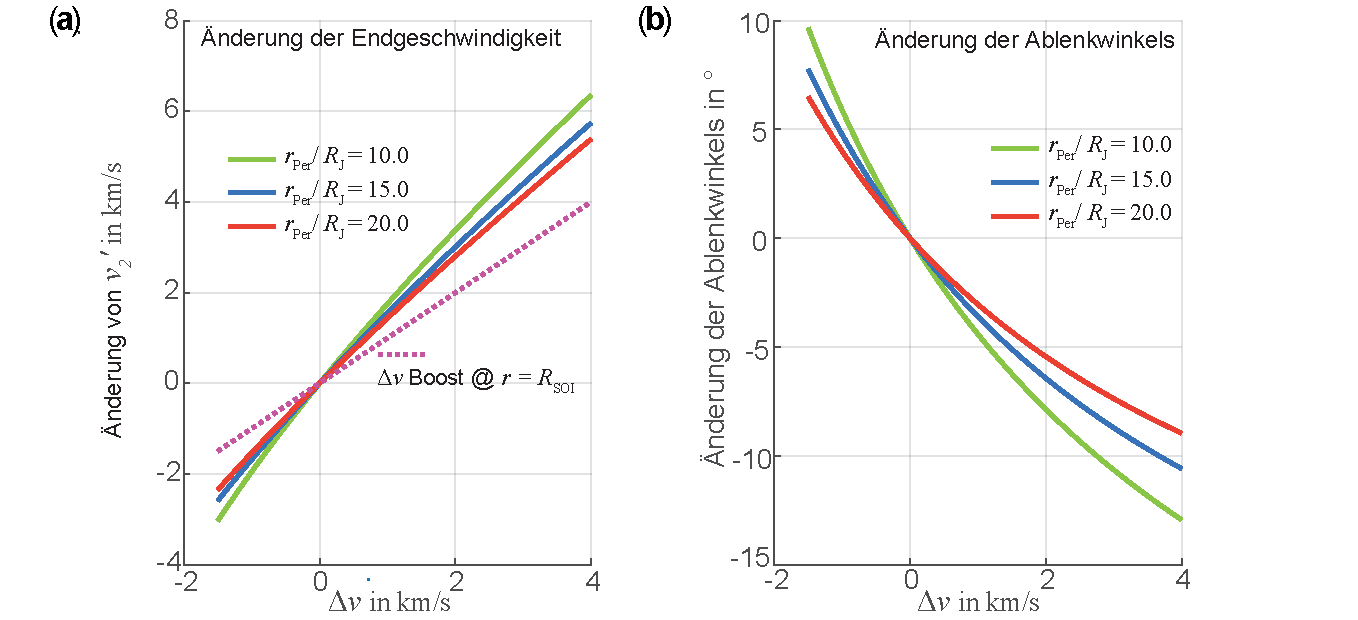
\includegraphics[width=\textwidth]{SwingByOberth01.pdf} 
	\caption[Geschwindigkeits- und Richtungs�nderung beim Gravity-Assist-Man�ver mit zus�tzlichem Schub.]{\fa Geschwindigkeits- und \fb Richtungs�nderung beim Gravity-Assist-Man�ver mit zus�tzlichem Schub am Beispiel Swing-By Jupiter. Man erkennt deutlich, dass der Geschwindigkeitszuwachs, wenn der Boost am Perizentrum erfolgt, deutlich gr��er ist als wenn dieser beim Eintreffen in die SOI des Jupiters erfolgen w�rde. Parameter siehe \mscr~ \mladynref{OberthSwingBy.m}.}
	\label{abb:adyn_swby03}
\end{figure}

\end{sol} 
\textcolor{blue} {$\rightarrow$ zur} \probref{adyn_swingby04}.\\
\noindent\rule[1ex]{\textwidth}{0.5pt} \newpage  \clearpage

%---------------------------------------------------------------------------------------------------


\begin{sol}{prob:adyn_raumfahrtschrott}\label{lsg:adyn_raumfahrtschrott} %Zusatz
\textbf{Raumfahrtschrott}\\

\begin{enumerate}
	\item\textit{\textbf{``Lebensdauer'' von Weltraumm�ll}}\\
	
Die Verweildauer von Weltraumm�ll in einer niedrigen Erdumlaufbahn
(\textit{Low Earth Orbi}t, LEO) wird im Wesentlichen durch den
atmosph�rischen Widerstand bestimmt.
Eine eindeutige Zuordnung \emph{Bahnh�he \(\to\) Lebensdauer} ist nicht
m�glich, da die Lebensdauer stark von
\begin{itemize}
  \item dem \emph{ballistischen Koeffizienten} \(A/m\) (projizierte Fl�che pro Masse),
  \item dem Aerodynamik-Koeffizienten \(C_\text{D}\),
  \item der zeitlich variablen Atmosph�rendichte \(\varrho(h,t)\) (stark variierend mit der Sonnenaktivit�t)
\end{itemize}
abh�ngt. Dennoch lassen sich f�r typische Objekte im All sinnvolle
Absch�tzungen angeben.

F�r ein Objekt der Masse \(m\) und Fl�che \(A\)
sei der aerodynamische Widerstand in erster N�herung (siehe Band I)
\begin{equation}
a_\text{drag}
= \frac{1}{2}\,\varrho(h)\,\,v^2\,C_\text{D}\,\frac{A}{m},
\end{equation}
wobei \(\varrho(h)\) die Atmosph�rendichte in H�he \(h\) und
\(v\) die Bahngeschwindigkeit ist.
Der Faktor \(C_\text{D} A/m\) wird h�ufig durch den
\emph{ballistischen Koeffizienten} charakterisiert:
\begin{equation}
B = \frac{m}{C_\text{D} A}
\quad\Leftrightarrow\quad
C_\text{D}\frac{A}{m} = \frac{1}{B}.
\end{equation}
Typische Werte f�r kleine Satelliten und gr��ere Tr�mmerobjekte liegen im Bereich
\begin{equation}
\frac{A}{m} \sim 10^{-2}\,\si{\meter^2\per\kilo\gram},
\end{equation}
also z.\,B.\ \(A=\SI{10}{\meter^2}\),~\(m=\SI{1000}{\kilo\gram}\)
bei \(C_\text{D} \approx 2.2\).\\


Wir benutzen das exponentielles Atmosph�renmodell (siehe \kap{adyn_drag}).
In guter N�herung kann man die Atmosph�rendichte im LEO
durch ein Exponentialgesetz beschreiben:
\begin{equation}
\varrho(h)
= \varrho_\mathrm{ref}\,\exp\!\left(-\frac{h-h_\mathrm{ref}}{H}\right),
\label{eq:rhoexp}
\end{equation}
wobei \(\varrho_\mathrm{ref}\) eine Referenzdichte bei H�he \(h_\mathrm{ref}\)
und \(H\) eine feste Skalenh�he ist. In einem verbesserten Modell ist \(H\) h�hen- und
zeitabh�ngig und \(\varrho(h,t)\) h�ngt wie erw�hnt stark von der Sonnenaktivit�t ab;
Gleichung~\eqref{eq:rhoexp} ist daher nur ein sehr einfaches Modell.

F�r die Dynamik im Orbit betrachten wir eine einfache Kreisbahn mit Bahnradius $a = R_\text{\earth} + h$, wobei $R_\text{\earth}$ der Erdradius ist.
Die Bahnenergie pro Masse lautet
\begin{equation}
\varepsilon = -\frac{\mu}{2a}
\end{equation}
mit dem Standardgravitationsparameter \(\mu = GM_\text{\earth}\), wobei $M_\text{\earth}$ die Masse der Erde ist.

Durch den Drag wird Energie dissipiert. Die �nderungsrate der
Energie ist $\D \varepsilon /\D t = \mathbf{a}_\text{D}\cdot\mathbf{v} = - a_\text{D}\,v$, da der Widerstand entgegengesetzt zur Geschwindigkeit wirkt.
Andererseits gilt
\begin{equation}
\frac{\mathrm d\varepsilon}{\mathrm d t}
= \frac{\mathrm d}{\mathrm d t}\left(-\frac{\mu}{2a}\right)
= \frac{\mu}{2a^2}\,\frac{\mathrm d a}{\mathrm d t}.
\end{equation}
Damit folgt
\begin{equation}
\frac{\mu}{2a^2}\,\frac{\mathrm d a}{\mathrm d t}
= - a_\text{D}\,v.
\end{equation}
F�r eine Kreisbahn ist $v = \sqrt{\mu/a}$.
Setzt man den Ausdruck f�r \(a_\text{D}\) ein,
\begin{equation}
a_\text{drag}
= \frac{1}{2}\,\varrho(h)\,v^2\,C_\text{D}\,\frac{A}{m},
\end{equation}
so erh�lt man
\begin{equation}
\frac{\mu}{2a^2}\,\frac{\mathrm d a}{\mathrm d t}
= - \frac{1}{2}\,\varrho(h)\,v^3\,C_\text{D}\,\frac{A}{m}.
\end{equation}
Einsetzen von \(v^3 = \left(\mu/a\right)^{3/2}\) liefert
\begin{equation}
\frac{\mathrm d a}{\mathrm d t}
= - \varrho(h)\,C_\text{D}\,\frac{A}{m}\,\sqrt{\mu}\,\sqrt{a}.
\label{eq:adot}
\end{equation}
Da \(h = a - R_\text{\earth}\) ist, h�ngt \(\varrho\) �ber \eqref{eq:rhoexp}
implizit von \(a\) ab. Gleichung~\eqref{eq:adot} l�sst sich numerisch integrieren. Aus einer Starth�he \(h_0\) berechnet man die Zeit bis zu einer
Reentry-H�he \(h_\text{reentry}\) (\zb \SI{122}{\kilo\meter}).\\

Als Gr��enordnungen der Lebensdauer erhalten wir mit 
einem typischen ballistischen Koeffizienten
\(A/m\sim 10^{-2}\,\si{\meter^2\per\kilo\gram}\) und
des erq�hnten groben Modells der Erd-Atmosph�re folgende Werte:

\begin{itemize}
  \item \(h_0 \approx \SI{300}{\kilo\meter}\):
        Lebensdauer von Monaten bis \ca \(\SI{1}{Jahr}\).
  \item \(h_0 \approx \SI{400}{\kilo\meter}\):
        typische Lebensdauer einiger Jahre (\zb~\ca 3-5~ Jahre).
  \item \(h_0 \approx \SI{500}{\kilo\meter}\): \ca 10-20~Jahre.
  \item \(h_0 \approx \SI{600}{\kilo\meter}\): mehrere Jahrzehnte.
  \item \(h_0 \approx \SI{800}{\kilo\meter}\): Jahrhunderte, da die Atmosph�rendichte sehr gering ist.
  \item \(h_0 \gtrsim \SI{1000}{\kilo\meter}\): Jahrhunderte bis Jahrtausende; der atmosph�rischer Drag ist vernachl�ssigbar.
\end{itemize}

Diese Zahlen sind nur Gr��enordnungen. �nderungen der
Sonnenaktivit�t oder des ballistischen Koeffizienten k�nnen die
Lebensdauer leicht um Faktoren von \(2{-}10\) verschieben. 
%Sie entsprechen in etwa der Aussage in \cite{Krag2025}. Wir verweisen f�r Details auf \mscr{} \mladynref{Raumfahrtschrott.m}.\\
%F�r eine quantitative Beispielrechnung l�sst sich 
%Gleichung~\eqref{eq:adot} in Verbindung mit dem
%Exponentialmodell \eqref{eq:rhoexp} numerisch integrieren.
%Setzt man z.\,B.
%\begin{align*}
%\varrho_\mathrm{ref} &\sim 4\times10^{-12}\,\si{\kilo\gram\per\meter^3}
%\quad\text{bei}\quad h_\mathrm{ref} \approx \SI{400}{\kilo\meter},\\
%H &\sim \SI{60}{\kilo\meter},\\
%C_\text{D} &\approx 2{,}2,\qquad \frac{A}{m}\sim 10^{-2}\,\si{\meter^2\per\kilo\gram},
%\end{align*}
%so erh�lt man eine Kurve \(\,T(h_0)\,\) (Lebensdauer als Funktion der
%Starth�he), die qualitativ den oben genannten Gr��enordnungen entspricht.
%Eine Darstellung in doppelt-logarithmischer Form (logarithmische
%Skalierung in der Zeitachse) zeigt, dass die Lebensdauer mit der H�he
%sehr stark anw�chst.\\
%
%Zusammenfassen kann man sagen, das es keinen exakten Zusammenhang zwischen
%Bahnh�he und Lebensdauer gibt; der ballistische Koeffizient \(A/m\), der Widerstandsbeiwert \(C_\text{D}\) und die
%Sonnenaktivit�t spielen eine zentrale Rolle. In einer einfachen Absch�tzung erh�lt man 
%mit der Exponentialatmosph�re und typischen ballistischen Koeffizienten f�r die Verweildauer
%Gr��enordnungen von Jahren bei \(\sim\SI{400}{\kilo\meter}\) \bzw Jahrtausende bei \(\gtrsim\SI{1000}{\kilo\meter}\).

\item\textit{\textbf{Beseitigung von Weltraumm�ll mit Lasern}}\\
	
Wir betrachten nun ein ideales, kugelf�rmiges St�ck Weltraumm�ll
mit Durchmesser \(\SI{10}{\centi\meter}\) in einer kreisf�rmigen Bahn
in \(\SI{800}{\kilo\meter}\) H�he �ber der Erdoberfl�che.
Ziel ist es, durch Laserablation die Bahn so zu �ndern, dass
das Perig�um auf etwa \(\SI{300}{\kilo\meter}\) abgesenkt wird.
In dieser H�he ist der atmosph�rische Widerstand gro� genug,
dass das Objekt typischerweise innerhalb von deutlich weniger als 5 Jahren 
wieder in die Atmosph�re eintritt (genaue Lebensdauer
h�ngt vom Atmosph�renmodell und dem ballistischen Koeffizienten ab) und vergl�ht.

Wir wollen eine grobe Absch�tzung der erforderlichen Laserenergie
f�r die Verwendung von Laserablation zur Weltraumm�ll-Beseitigung machen.

\subparagraph{Orbitdynamik}

Wir modellieren die Erde mit Radius $R_\text{\earth} \approx \SI{6371e3}{\meter}$
und Standardgravitationsparameter
$\mu_\text{\earth} \approx \SI{3.986e14}{\meter^3\per\second^2}$.
Die Ausgangsbahn sei kreisf�rmig mit H�he $h_0 = \SI{800e3}{\meter}$, und damit $r_0 = R_\text{\earth} + h_0$.
Die Kreisbahngeschwindigkeit ist
\begin{equation}
v_{\text{K,0}}
= \sqrt{\frac{\mu_\text{\earth}}{r_0}}.
\end{equation}
Als Zielbahn soll eine elliptische Bahn mit Apog�um in \(\SI{800}{\kilo\meter}\)
und Perig�um in \(\SI{300}{\kilo\meter}\) angenommen werden:
\[
h_\text{P} = \SI{300e3}{\meter},\quad
r_\text{P} = R_\text{\earth} + h_\text{P},\quad
r_\text{A} = r_0.
\]
Die gro�e Halbachse dieser lautet dann $a = (r_\text{P} + r_\text{A})/2$.
Die Geschwindigkeit im Apog�um dieser elliptischen Bahn ergibt sich
aus der \textit{vis-viva-Gleichung}\index{vis-viva-Gleichung} \eqref{eq:hm_vis-viva}:
\begin{equation}
v_\text{A}
= \sqrt{\mu_\text{\earth}\left(\frac{2}{r_\text{A}} - \frac{1}{a}\right)}.
\end{equation}
Wir brauchen  also am Apog�um eine retrograde Geschwindigkeits�nderung \(\Delta v\), um von der
kreisf�rmigen in die elliptische Bahn zu wechseln:
\begin{equation}
\Delta v = v_{\text{K,0}} - v_\text{A}.
\end{equation}
Mit den Zahlenwerten erhalten wir
%\begin{align}
%r_0 &= R_\text{earth} + \SI{800e3}{\meter},\\
%r_\text{P} &= R_\text{earth} + \SI{300e3}{\meter},\\
%a &= \frac{r_0 + r_\text{p}}{2}.
%\end{align}
%Damit erh�lt man numerisch
$ v_{\text{c,0}} \approx \SI{7456}{\meter\per\second},\,\,v_\text{A} \approx \SI{7320}{\meter\per\second},\,\, \Delta v \approx \SI{136}{\meter\per\second}$.
Dieses \(\Delta v\) gen�gt, um das Perig�um auf \ca \(\SI{300}{\kilo\meter}\)
abzusenken. 
%Noch niedrigere Zielh�hen (z.\,B. \(\SI{200}{\kilo\meter}\))
%w�rden ein etwas gr��eres \(\Delta v\) erfordern (Gr��enordnung
%\(\sim \SI{160}{\meter\per\second}\)).\\

Wir nehmen an, dass das Objekt eine Kugel aus Aluminium
mit Durchmesser \(d = 2r = \SI{10}{\centi\meter}\) ist.
%Das Volumen der Kugel ist
%\begin{equation}
%V = \frac{4}{3}\pi r^3.
%\end{equation}
Mit einer typischen Dichte f�r Aluminium von
\(\varrho \approx \SI{2700}{\kilo\gram\per\meter^3}\) ist die Masse
$m = \varrho V \approx \SI{1.4}{\kilo\gram}$.
%In der Realit�t kann die Masse je nach Geometrie und Material
%stark variieren; \(\SI{1}{\kilo\gram}\) bis einige \(\SI{}{kg}\) f�r
%\(\sim\SI{10}{\centi\meter}\)-Objekte ist jedoch plausibel als Gr��enordnung.\\

Der f�r die Bahn�nderung notwendige Impuls ist
\begin{equation}
I_\text{ges} = m\,\Delta v \approx \SI{1.9e2}{\newton\second} \,.
\end{equation}

\subparagraph{Laserablation und Impuls-Kopplungskoeffizient}

Bei Laserablation wird eine d�nne Oberfl�chenschicht verdampft
und bildet einen Plasmastrahl. Der R�cksto� liefert den gew�nschten
Impuls. Als praktische Kenngr��e wird h�ufig der
\emph{Impuls-Kopplungskoeffizient} \(C_m\) verwendet:
\begin{equation}
C_\text{abl} = \frac{\Delta I}{E_\text{Laser}},
\end{equation}
also Impuls pro eingestrahlter Laserenergie. Die Einheit ist
\(\si{\newton\second\per\joule}\).

Typische Werte f�r \(C_\text{abl}\) bei Nanosekundenimpulsen im
\(\SI{1}{\micro\meter}\)-Bereich und geeigneten Energiewerten
liegen in der Gr��enordnung
\[
C_\text{abl}\sim 10^{-4} \dots 10^{-3}\,\si{\newton\second\per\joule},
\]
je nach Material, Wellenl�nge, Pulsdauer und Energie.

Die erforderliche Laserenergie zur Erzeugung des Gesamtimpulses
\(I_\text{ges}\) ist $E_\text{Laser} = I_\text{ges}/C_\text{abl}$.
Mit \(I_\text{ges} \approx \SI{1.9e2}{\newton\second}\) und
\(C_\text{abl} \approx \SI{3e-4}{\newton\second\per\joule}\) ergibt sich
\begin{align}
E_\text{Laser}
&\approx \frac{\SI{1.9e2}{}}{\SI{3e-4}{}}\,\SI{}{\joule} \approx \SI{6.4e5}{\joule} \approx \SI{0.64}{\mega\joule}\,.
\end{align}

F�r andere plausible Werte von \(C_\text{abl}\) ergibt sich z.\,B.
\begin{align*}
C_\text{abl} &= \SI{1e-4}{\newton\second\per\joule}
&&\Rightarrow&
E_\text{Laser} &\approx \SI{1.9e6}{\joule}
\approx \SI{1.9}{\mega\joule},\\
C_\text{abl} &= \SI{1e-3}{\newton\second\per\joule}
&&\Rightarrow&
E_\text{Laser} &\approx \SI{1.9e5}{\joule}
\approx \SI{0.19}{\mega\joule}.
\end{align*}

Wir erhalten also eine grobe Bandbreite von $E_\text{Laser} \sim 0.2 \dots 2\,\si{\mega\joule} $ f�r ein \(\SI{10}{\centi\meter}\)-Objekt mit \(\sim\SI{1.4}{\kilo\gram}\)
Masse und \(\Delta v \sim \SI{136}{\meter\per\second}\).

Setzen wir \(E_\text{Laser} \approx \SI{0.64}{\mega\joule}\) an,
so entspricht dies $E\text{el} = E_\text{Laser}/\eta$, wobei \(\eta\) der Gesamtwirkungsgrad vom Stromnetz bis zum
Zielobjekt ist (Laser-Wirkungsgrad, Strahlf�hrung, atmosph�rische
Verluste etc.). Selbst bei einem eher optimistischen Gesamtwirkungsgrad
$\eta \sim 10\%$ ergibt sich
\begin{equation}
E_\text{el} \approx \SI{1.8}{\kilo\watt\hour}\,.
\end{equation}
Das ist energetisch durchaus handhabbar, zumal sich die Ablation
�ber viele einzelne Impulse und zahlreiche Uml�ufe verteilen kann.\\

In einem realistischen Szenario w�rde man das Objekt bei jedem
�berflug des Laserstandorts (bzw.\ des Laser-Satelliten)
f�r kurze Zeit im Fokus haben und pro Passage eine gewisse Anzahl
von Impulsen einbringen. Der Gesamtimpuls von \ca
\(\SI{200}{\newton\second}\) kann also auf viele hundert oder tausende
Impulse verteilt werden, etwa in der Gr��enordnung
\begin{equation}
\Delta I_\text{pro Impuls} \sim 10^{-2} \dots 10^{-1}\,\si{\newton\second},
\end{equation}
je nach Impulsenergie.\\

Die gemachte Absch�tzung enth�lt
mehrere idealisierende Annahmen:
\begin{itemize}
  \item Das Objekt ist eine homogene Aluminiumkugel; reale Tr�mmer
        haben komplexe Geometrie und Materialkombinationen.
  \item Der Impuls-Kopplungskoeffizient \(C_\text{abl}\) h�ngt stark von
        verschiedenen Parametern ab.
  \item Die Orbitdynamik ist idealisiert (keine St�rungen, kein zus�tzlicher aerodynamischer Drag
        w�hrend der Absenkphase).
\end{itemize}

Bei der Bahn�nderung von Weltraumm�ll durch Laserbestrahlung stellt sich die Frage, ob neben dem R�cksto� durch die Ablationsplasmawolke auch der reine Photonenimpuls des Laserstrahls ber�cksichtigt werden muss.\\
Im eigentlichen Ablationsregime ist der Photonenimpuls in der Regel gegen�ber dem Ablationsr�cksto� vernachl�ssigbar. Unterhalb der Ablationsschwelle kann er dagegen der f�hrende Effekt sein. Wir wollen das quantitativ absch�tzen:
Allgemein kann man mit einem dimensionslosen Kopplungsfaktor \(C_R\) der Impuls�bertrag  als (siehe Band V):
\begin{align}
	\Delta I_\text{photon} = C_\text{R} \frac{E_\text{Laser}}{c}\, \qquad 1 \le  C_\text{R}R \le 2
\end{align}
f�r den Bereich zwischen idealer Absorption und idealer Spiegelung schreiben.
Daraus folgt f�r den Impuls pro Joule bei Absorption
\[
\lk \frac{\Delta I_\text{photon}}{E_\text{Laser}}\rk_\gamma \approx \SI{3.33e-9}{\newton\second\per\joule}\,,
\]
und bei perfekter Reflexion maximal der doppelte Betrag, was sehr klein ist.
Das Verh�ltnis von Ablationsimpuls zu Photonenimpuls ist
\[
\frac{\Delta I_\text{abl}}{\Delta I_\text{photon}} = \frac{C_\text{abl} E_\text{Laser}}{C_\text{R} E_\text{Laser}/c} = \frac{C_\text{abl}}{C_\text{R}}c\,.
\]
Mit $C_\text{abl} = \SI{1e-5}{\newton\second\per\joule}$ erh�lt man f�r $\Delta I_\text{abl}/\Delta I_\text{photon}$ einen Wert von \ca $\SI{3e3}{}$.
Der Ablationsr�cksto� ist also typischerweise um drei bis vier Gr��enordnungen gr��er als der reine Photonenimpuls.\\

Trotz unserer gemachten Vereinfachungen liefert die Rechnung eine sinnvolle
Gr��enordnung: F�r ein \(\SI{10}{\centi\meter}\)-Objekt in \(\SI{800}{\kilo\meter}\)
H�he liegt die erforderliche Laserenergie zur Absenkung des Perig�ums
auf etwa \(\SI{300}{\kilo\meter}\) typischerweise im Bereich einiger
\(\SI{}{\mega\joule}\) auf dem Zielobjekt, was technisch prinzipiell
machbar ist, wenn man die Ablation �ber viele Uml�ufe verteilt. In Bezug auf reine Energiegr��enordnungen erscheint
ein Laser-basiertes Deorbiting einzelner \(\SI{10}{\centi\meter}\)-Objekte
prinzipiell realistisch. Die eigentlichen Herausforderungen liegen eher
in Strahlf�hrung, Zielverfolgung und Systemkomplexit�t.
Insbesondere haben wir in unseren Rechnungen unber�cksichtigt gelassen, wie die Laserenergie von der Erde so zum Tr�mmerobjekt gebracht werden kann, \dh ausgerichtet und fokussiert werden kann, dass die gesamte \bzw ein Gro�teil der von der Erde abgestrahlten Energie das relativ kleine Tr�mmerobjekt trifft. Mit solchen, im Wesentlichen optischen Fragen, wollen wir uns n�her im Band V besch�ftigen.  

%Nicht zuletzt soll erw�hnt werden, dass es f�r die Methode noch eine  Reihe rechtlicher und politischer Rahmenbedingungen zu kl�ren gilt.

%Zusammenfassung 
%
%\begin{itemize}
  %\item Ben�tigtes \(\Delta v\) zur Absenkung des Perig�ums von
        %\(\SI{800}{\kilo\meter}\) auf \(\SI{300}{\kilo\meter}\):
        %\(\Delta v \approx \SI{136}{\meter\per\second}\).
  %\item Masse eines idealisierten \(\SI{10}{\centi\meter}\)-Aluminiumfragments:
        %\(m \approx \SI{1.4}{\kilo\gram}\).
  %\item Gesamtimpulsbedarf:
        %\(I_\text{ges} \approx \SI{2e2}{\newton\second}\).
  %\item Bei typischen Werten f�r den Impuls-Kopplungskoeffizienten
        %\(C_m \sim 10^{-4} \dots 10^{-3}\,\si{\newton\second\per\joule}\)
        %ergibt sich eine ben�tigte Laserenergie auf dem Zielobjekt von
        %\[
        %E_\text{Laser} \sim 0{,}2 \dots 2\,\si{\mega\joule}.
        %\]
%\end{itemize}
%
\end{enumerate}

\end{sol} 
\textcolor{blue} {$\rightarrow$ zur} \probref{adyn_raumfahrtschrott}.\\
\noindent\rule[1ex]{\textwidth}{0.5pt} 

%---------------------------------------------------------------------------------------------------

\newpage
\begin{sol}{prob:adyn_proxima_centauri}\label{lsg:adyn_proxima_centauri} %Zusatz
\textbf{Starshot and Starlight}\\


Wir verweisen auf \cite{Umrigar2025} und danken den Autoren f�r dieses instruktive physikalische Problem.\\

\end{sol} 
\textcolor{blue} {$\rightarrow$ zur} \probref{adyn_proxima_centauri}.\\
\noindent\rule[1ex]{\textwidth}{0.5pt} 



%---------------------------------------------------------------------------------------------------

\newpage
\begin{sol}{prob:adyn_waterrocket}\label{lsg:adyn_waterrocket} %Zusatz
\textbf{Wasserrakete}\\

Gegeben sind folgende Parameter:
\begin{itemize}
  \item Wasservolumen $V_\text{W0}$, Luftvolumen �ber dem Wasser $V_\text{A0}$, Flaschenvolumen $V_\text{F}=V_\text{W0}+V_\text{A0}$.
  \item Druck der komprimierten Luft $p_0$ als Absolutdruck.
  \item D�sendurchmesser $d_\text{N}$ mit Querschnitt $A_\text{N}=\pi(d_\text{N}/2)^2$.
  \item Abschusswinkel $\theta$ (konstant als Schubrichtung angenommen).
  \item Trockenmasse $m_\mathrm{F}$ (Flasche+Nase+Finnen), aerodynamische Parameter $C_\text{D}$ und Referenzfl�che $A_\mathrm{ref}$.
\end{itemize}

Konstanten:
Wasserdichte $\varrho_\text{W}\approx 1000\,\mathrm{kg/m^3}$, Luftdichte $\varrho_\mathrm{A}\approx 1.2\,\mathrm{kg/m^3}$,
adiabatischer Exponent der Luft $\gamma\approx 1.4$,
Umgebungsdruck $p_\mathrm{Luft}\approx 101325\,\mathrm{Pa}$.
Der Ausflussbeiwert der D�se liege $C_\text{D,N}$ im Intervall $[0.8,0.95]$.

In der Wasser-Schubphase (Blowdown), \dh w�hrend Wasser ausstr�mt, vergr��ert sich das Luftvolumen $V_\text{A}(t)$, und der Flaschendruck f�llt adiabatisch:
\begin{equation}
p(t)=p_0\left(\frac{V_\text{A0}}{V_\text{A}(t)}\right)^\gamma.
\end{equation}
Der antreibende Differenzdruck ist $\Delta p(t)=\max(p(t)-p_\mathrm{L},0)$.

F�r die Strahlgeschwindigkeit (wir nehmen die Bernoulli-L�sung (siehe Band I) mit Ausflussbeiwert gilt
\begin{equation}
v_\text{ex}(t)=C_\text{D,N}\sqrt{\frac{2\,\Delta p(t)}{\varrho_\text{W}}}.
\end{equation}
Damit folgen Volumenstrom \bzw  Massenstrom des Wassers:
\begin{equation}
\dot V(t)=A_n v_\text{ex}(t), ~~ \rightarrow~~ \dot m_\text{W}(t)=\varrho_\text{W} A_\text{N} v_\text{ex}(t).
\end{equation}
Eine einfache Schubn�herung in der Wasserphase ist die Impulsbilanz
\begin{equation}
T(t)\approx \dot m_\text{W}(t)\, v_\text{ex}(t).
\end{equation}
Diese ist gerechtfertigt, da der zus�tzliche Druckterm $(p_\text{ex}-p_\mathrm{amb})A_n$ bei freiem Wasserstrahl meist klein gegen�ber $\dot m v_\text{ex}$ ist. 
Die Luftvolumen�nderung ist identisch mit dem abgeflossenen Wasservolumen:
\begin{equation}
\dot V_\text{A}(t)=\dot V(t)=A_n v_\text{ex}(t).
\end{equation}
Die Wasserphase endet bei $V_\text{A}(t)=V_\text{F}$ (Wasser ist leer) oder wenn $\Delta p(t)=0$.
Die Wassermasse ist $m_w(t)=\varrho_w V_\text{W}(t)$ und f�llt mit
\begin{equation}
\dot m_\text{W}(t)=-\varrho_\text{W} A_\text{N} v_\text{ex}(t).
\end{equation}
Die Gesamtmasse sei (w�hrend der Wasserphase)
\begin{equation}
m(t)=m_\mathrm{F}+m_\text{W}(t)+m_\mathrm{A},
\end{equation}
wobei $m_\mathrm{A}$  als konstant angenommen werden kann.

Der aerodynamischer Widerstand wird quadratisch angesetzt (wir haben nach einfacher Absch�tzung eine gro�e Reynolds-Zahl, die Turbulenz ergibt):
\begin{equation}
\mathbf{F}_\text{D}=\frac12\varrho_\mathrm{air} C_\text{D} A_\mathrm{ref} \, |\vec{v}|\,\vec{v}.
\end{equation}
Die Schubrichtung wird als konstant entlang des Abschusswinkels $\theta$ angenommen (Das setzt voraus, dass zumindest in der Schubphase die Rakete ihrer Abschussrichtung beibeh�lt,  genauer w�re eigentlich wenn Schubrichtung der Tangente an die Bahn entspricht.)
\begin{equation}
\vec{T}(t)=T(t)\begin{pmatrix}\cos\theta\\ \sin\theta\end{pmatrix}.
\end{equation}
Dann lautet die Bewegungsgleichung:
\begin{equation}
m(t)\, \dot{\mathbf{v}}=\vec{T}(t)-\vec{F}_\text{D} - m(t)\,g\begin{pmatrix}0\\1\end{pmatrix}.
\end{equation}
Die Numerische Integration erfolgt in Zeitschritten $\Delta t$ mit explizitem Euler-Verfahren oder der \matlab~\odevf-Rotine.
Ausgegeben werden die Trajektorien $(x(t),y(t))$, $(t,z(t))$, die maximale H�he $z_\mathrm{max}$, die Flugzeit $t_\mathrm{impact}$ und die Reichweite $x(t_\mathrm{impact})$ (bei $z=0$). Ergebnisse haben wir f�r die Werte unserer Modellraket (Tabelle \ref{tab:adyn_param_wasserrakete}) zeigen wir in \figref{adyn_WaterRocket}.\\
\begin{table}%tab1
\smallskip
\begin{tabular}{L{4cm}L{4cm}}
\svhline\noalign{\smallskip}
\noalign{\smallskip}
\textbf{Gr��e} & \textbf{Wert} \\
\noalign{\smallskip}\svhline\noalign{\smallskip}
Wasservolumen bei $t=0$ & $0.375\,\mathrm{l}$ \\
Luftvolumen bei $t=0$   & $0.375\,\mathrm{l}$ \\
Masse der Flasche       & $70.00\,\mathrm{g}$ \\
Druck bei $t=0$         & $650000.00\,\mathrm{Pa}$ \\
D�sendurchmesser        & $5.00\,\mathrm{mm}$ \\
$C_\text{D}$-Wert       & $0.40$ \\
Querschnitt             & $19.63\,\mathrm{cm^2}$ \\
Winkel                  & $55.00^\circ$ \\
\hline
Reichweite              & $86.1\,\mathrm{m}$ \\
Maximale H�he           & $33.7\,\mathrm{m}$ \\
Flugzeit                & $5.79\,\mathrm{s}$ \\
\noalign{\smallskip}
\svhline\noalign{\smallskip}
\end{tabular}
\caption{Parameter und Messwerte der Wasserrakete}
\label{tab:adyn_param_wasserrakete}
\end{table}
\begin{figure}
	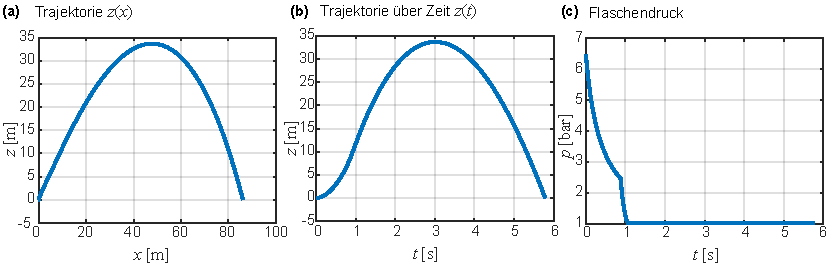
\includegraphics[scale=1]{WaterRocket.pdf} 
	\caption[Trajektorie einer Wasserrakete.]{Trajektorie einer Wasserrakete. Parameter siehe Tabelle \ref{tab:adyn_param_wasserrakete} und \mscr~ \mladynref{WaterRocket.m}.}
	\label{abb:adyn_WaterRocket}
\end{figure}

Bei der numerischen Integration m�ssen wir auf  einen ``stetigen'' �bergang zwischen Wasser- und Gasphase achten, denn im einfachen Modell wird beim Erreichen von $m_\text{W}=0$ abrupt von der Wasser-Schubformel auf die Gas-Schubformel umgeschaltet. Dadurch w�rde im Schub-Zeit-Diagramm unter Umst�nden 
eine unphysikalisch Diskontinuit�t auftreten. Zur numerischen Regularisierung verwenden wir deshalb eine kleine �bergangszone f�r sehr kleine Restwassermassen. Sei
$ m_{\text{W}0}=\varrho_\text{W} V_{\text{W}0}$ die Anfangswassermasse und $\varepsilon \ll 1$ ein kleiner Bruchteil, \zb $0.02$, dann wird f�r
$m_\text{W} \le \varepsilon\, m_{\text{W}0}$
ein ``glatter'' Mischfaktor
\begin{align}
	w = \frac12 \lek 1+\cos\!\lk \pi \lk 1-\frac{m_\text{W}}{\varepsilon m_{\text{W}0}}\rk \rk \rek
\end{align}
verwendet. Dann gilt:
\[
w=1 \quad \text{bei} \quad m_\text{W}=\varepsilon m_{\text{W}0}, \qquad w=0 \quad \text{bei} \quad m_\text{W}=0\,.
\]
Der Schub wird in dieser Zone als gewichtete Summe geschrieben:
$T = w\,T_\mathrm{W} + (1-w)\,T_\mathrm{A}$, Analog kann auch der Massenstrom gegl�ttet werden:
\[
\dot m = w\,\dot m\text{W} + (1-w)\,\dot m_\text{A}.
\]
Diese Vorgehensweise ist in erster Linie eine numerische Regularisierung und kein
vollst�ndiges physikalisches Zweiphasenmodell, f�hrt aber zu einer realistischen und numerisch stabilen
Schubkurve.\\

Die �bereinstimmung der numerischen Rechnung mit den Beobachtungen ist damit relativ gut, insbesondere wenn man die gemachten groben N�herungen ber�cksichtigt.\\

Wir wollen das Ganze jetzt noch mit einer so genannten Fehlerlandkarte (\textit{Error-Map}) �berpr�fen. Das Ziel ist, aus den experimentellen Messdaten Reichweite, maximale H�he, Flugzeit 
($R_{\mathrm{exp}}, H_{\mathrm{exp}}$ und $T_{\mathrm{exp}}$ )
die plausiblen unbekannten Modellparameter zu bestimmen. 
Im unserem Fall werden als freie Parameter der aerodynamische Widerstandsbeiwert  $C_\text{D}$ und der absolute Anfangsdruck $p_0$ genommen. 
Alle �brigen Gr��en, insbesondere die geometrischen Gr��en der Rakete, werden als bekannt angenommen.
Die Methode basiert auf einer systematischen Abtastung des Parameterraums und der Bewertung der jeweiligen Parameterkombination durch eine Fehlerfunktion.
Das physikalische Modell, im \mscr{}~ durch 
$\textcolor{mygreen}{\texttt{waterRocketSim}}$ 
realisiert, definiert eine Abbildung der Art
\begin{align}
	(C_\text{D}, p_0) ;\longmapsto; \lk R_{\mathrm{sim}}, H_{\mathrm{sim}}, T_{\mathrm{sim}}\rk \,.
\end{align}
Zum Vergleich zwischen Simulation und Messung werden relative Fehler definiert:
\begin{align*}
	e_R &= \frac{R_{\mathrm{sim}} - R_{\mathrm{exp}}}{R_{\mathrm{exp}}}\,,\quad e_H = \frac{H_{\mathrm{sim}} - H_{\mathrm{exp}}}{H_{\mathrm{exp}}}\,,\quad
	e_T = \frac{T_{\mathrm{sim}} - T_{\mathrm{exp}}}{T_{\mathrm{exp}}}\,.
\end{align*}
Diese Normierung hat den Vorteil der dimensionslosen Darstellung und der gleichen Gewichtung der Messwerte unabh�ngig von der Gr��enordnung.

\begin{figure}
	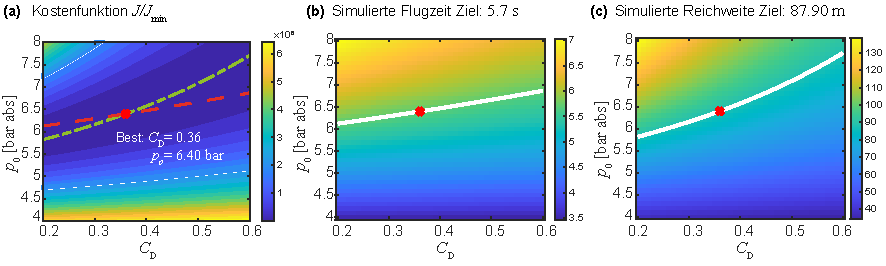
\includegraphics[scale=1]{WaterRocket02.pdf} 
	\caption[Error-Map einer Wasserrakete f�r die Variablen Parameter $p_0$ und $C_\text{D}$.]{Error-Map einer Wasserrakete f�r die variablen Parameter $p_0$ und $C_\text{D}$. \fa Error-Map mit Schnittpunkt Flugzeit und Reichweite als Messwerte der Wasserrakete \fb Zielsimulation auf die Messwert Flugzeit der Wasserrakete, \fc Zielsimulation auf die Messwert Reichweite der Wasserrakete. Parameter siehe Tabelle \ref{tab:adyn_param_wasserrakete} und \mscr~ \mladynref{WaterRocket.m}.}
	\label{abb:adyn_WaterRocket02}
\end{figure}

Die Fehler werden zu einer skalaren Kostenfunktion kombiniert:
\begin{align}
	J(C_\text{D},p_0) = w_R e_R^2 + w_H e_H^2 + w_T e_T^2\,~~\text{mit Gewichtungsfaktoren}~~w_R, ~ w_H, ~ w_T \ge 0\,.
\end{align}
$J=0$ entspricht perfekter �bereinstimmung, kleine Werte von $J$ bedeuten gute Anpassung.
Der Parameterraum wird auf einem Gitter diskretisiert, woraus sich ein zweidimensionales Raster
$[C_{\text{D},i}, p_{0,j}] $ f�r $i=1,\dots,N,~ j=1,\dots,M$ ergibt.
F�r jedes Gitterelement wird die Simulation durchgef�hrt und aus den relativen Fehlern $e_R, e_H, e_T$ die Kostenfunktion ausgewertet:
Aus der erhaltenen Matrix ergibt sich der beste Parametersatz durch Minimierung.
In der Error-Map wird die Funktion $J(C_\text{D},p_0)$ \zb durch eine Farbkarte (\textit{Heatmap}) dargestellt.
Zus�tzlich werden h�ufig geplottet $R_{\mathrm{sim}}(C_\text{D},p_0)$, $T_{\mathrm{sim}}(C_\text{D},p_0)$ und $H_{\mathrm{sim}}(C_\text{D},p_0)$.
Besonders aussagekr�ftig sind die Konturen $R_{\mathrm{sim}} = R_{\mathrm{exp}}$, $T_{\mathrm{sim}} = T_{\mathrm{exp}}$ und $H_{\mathrm{sim}} = H_{\mathrm{exp}}$.
Schnittpunkte dieser Kurven im Parameterraum entsprechen konsistenten L�sungen, mehrere Schnittpunkte bedeuten Nicht-Eindeutigkeit und  keine Schnittpunkte deuten auf Modellabweichungen hin.\\

Die Error-Map ist ein zentrales Werkzeug zur Modellvalidierung und Parameteridentifikation und liefert eine hilfreiche diskrete Approximation der Funktion $J(C_\text{D},p_0)$ dar, welche den Abstand zwischen Simulation und Experiment misst.
Sie erlaubt eine visuelle Analyse des Parameterraums, eine Bestimmung optimaler Parameter und die Identifikation von Unsicherheiten und Korrelationen.\\

\subparagraph{Modellverfeinerungen und zus�tzliche Problemstellungen:}

In einer Verfeinerung des Modells k�nnte man ber�cksichtigen:
\begin{enumerate} [1)]
	\item die Beschreibung der Rakete als starren K�rper mit ver�nderlichen Schwerpunkt, 
	\item den Pitch (Nickbewegung) der Richtung des Schubs durch die Wirkung Schwerkraft/Reibung auf die Rakete,
	\item den Auftrieb der Rakete und
	\item die Rotation der Rakete um die L�ngsachse (hervorgerufen durch die seitlichen ``Flossen'').
\end{enumerate}

Eine weitere sch�ne �bung ist der Vergleich mit der Trajektorie eines schr�gen Wurfs, der die gleiche H�he und Reichweite erreicht. 
Man vergleiche insbesondere die dazu notwendige  Abwurfgeschwindigkeit. (Wir verweisen auch auf die �bung 1.41 in Band I Mechanik).
Wir finden interessanterweise, dass man bei einer Abwurfgeschwindigkeit von udn einem Abwurfwinkel eine Trajektorie $z(x)$ erh�lt, die in etwa mit der Trajektorie der Wasserrakete �bereinstimmt und zwar sowohl bei Scheitelh�he als auch Reichweite.
Das Zeitverhalten ist aber leicht unterschiedlich (die Rakete muss ja erst beschleunigt werden), so dass der Wurf eine um 0.5 s verk�rzte Flugzeit hat. Siehe dazu die \mscr{}e \mladynref{WaterRocket.m} und \mladynref{WaterRocketVergleichWurf.m}.

%Wir wollen die Punkte 1) bis 3) gemeinsam angehen und die Rakete nicht mehr als Punktmasse behandeln, sondern als starren K�rper (in der $x$-$z$-Ebene).
%Dadurch k�nnen zus�tzlich zur translatorischen Bewegung auch die Orientierung und die Nickbewegung beschrieben werden.
%
%Das Modell umfasst:
%\begin{itemize}
%\item Translation des Schwerpunkts in der Ebene $(x,z)$,
%\item Rotation der Rakete mit Winkel $\theta$,
%\item Winkelgeschwindigkeit $\omega=\dot\theta$,
%\item zeitabh�ngige Gesamtmasse $m(t)$,
%\item zeitabh�ngigen Schwerpunkt $x_{CG}(t)$ entlang der Raketenachse,
%\item zeitabh�ngiges Tr�gheitsmoment $I_{CG}(t)$.
%\end{itemize}
%
%Der Zustandsvektor sei
%\[
%\vec{Y}(t)= \lek x, z, v_x, v_z, \theta, \omega, m_\text{W},  m_\text{A} \rek^\text{T}\,.
%\]
%Dabei ist $\theta$ die Orientierung der Raketenachse gegen die $x$-Achse und ,
%$\omega$ die Nickrate. Die anderen Parameter wurden bereits oben eingef�hrt.
%Die Raketenachse ist durch den Einheitsvektor
%\[
%\vec e_\text{R}=
%\begin{pmatrix}
%\cos\theta\\
%\sin\theta
%\end{pmatrix}
%\]
%gegeben.
%Ein dazu senkrechter Einheitsvektor ist
%\[
%\vec e_n=
%\begin{pmatrix}
%-\sin\theta\\
%\cos\theta
%\end{pmatrix}.
%\]
%Die Geschwindigkeit des Schwerpunkts ist
%\[
%\vec v=
%\begin{pmatrix}
%v_x\\
%v_z
%\end{pmatrix},
%\qquad
%V=\|\mathbf v\|=\sqrt{v_x^2+v_z^2}.
%\]
%Der Flugbahnwinkel (siehe \kap{}) ist $\gamma=\operatorname{atan2}(v_y,v_z)$.
%Der Anstellwinkel (ebenfalls Verweis auf\kap{}) der Rakete relativ zur Flugrichtung wird definiert als $\alpha=\theta-\gamma$.
%F�r kleine Winkel ist $\alpha$ der zentrale aerodynamische P
%%Die Gesamtmasse ist
%%\[
%%m(t)=m_{\mathrm{F}} + m_\text{W}(t) + m_\text{W}(t) + m_a(t).
%%\]a(t).
%%\]
%%
%Die Lage des Schwerpunkts entlang der Raketenachse werde durch $x_\text{S}(t)$
%beschrieben. Sie kann aus den Teilmassen berechnet werden:
%\[
%x_\text{S}(t)=\frac{\sum_i m_i(t)x_i}{\sum_i m_i(t)},
%\]
%wobei man typischerweise die Rakete in die Bestandteile trockene Flasche, Wasserf�llung, Luft, Nase und Flossen zerlegt.
%Das Tr�gheitsmoment um den Schwerpunkt ist
%\[
%J_\text{S}(t)=\sum_i \lk J_i^{(\mathrm{eig})} + m_i(t) \lek (x_i-x_\text{S}(t)\rek^2\rk\,.
%\]
%Es wirken im Wesentlichen vier Kr�fte:
%\begin{enumerate} [(a)]
	%\item Schwerkraft\\
			%\[
		%\mathbf F_g=
		%\begin{pmatrix}
		%0\\
		%-\,m(t)g 
		%\end{pmatrix}.\]
	%\item Schub\\
	%Der Schub wirkt entlang der Raketenachse: $\mathbf F_T = T(t)\,\vec e_\text{R}$.
	%\item Luftwiderstand\\
	%Der Widerstand wirkt entgegen der Flugrichtung:
		%\[
		%\mathbf F_D
		%=
		%-\frac12 \rho_{\mathrm{air}} V^2 A_{\mathrm{ref}} C_\text{D} \,\vec e_v,
		%\]
		%wobei $\mathbf e_v=\frac{\mathbf v}{V}$ f�r $V>0$.
	%\item Normalkraft\\
		%Die aerodynamische Normalkraft wird f�r kleine Anstellwinkel modelliert durch $N=\frac12 \rho_{\mathrm{A}} V^2 A_{\mathrm{ref}}\, C_{N\alpha}\,\alpha$. Sie wirkt senkrecht zur Raketenachse, \dh $\vec{F}_N = N\,\vec{e}_n$.
%\end{enumerate}
%
%Die Translation des Schwerpunkts folgt der Newton-Bewegungsgleichung. 
%\begin{align}
	%m(t)\,\dot{\mathbf v} &= \mathbf F_T + \mathbf F_D + \mathbf F_N + \mathbf F_g\,\\
%\end{align}
%\bzw in Komponentenschreibweise:
%\begin{align}
%\begin{split}
	%\dot x   &= v_x\,,\\
	%\dot z 	 &= v_z\,,\\
	%\dot v_x &= \frac{F_{T,x}+F_{D,x}+F_{N,x}}{m(t)}\,,\\
	%\dot v_z &= \frac{F_{T,y}+F_{D,y}+F_{N,y}}{m(t)} - g\,.
%\end{split}
%\end{align}
%Die Rotationsgleichung um den Schwerpunkt lautet
%\begin{align}
	%I_\text{S}(t)\,\dot\omega = M(t)~~~\text{mit}~~~\dot\theta=\omega\,.
%\end{align}
%Das dominierende Drehmoment ist h�ufig das aerodynamische Nickmoment $M_N = N\,(x_\text{CP}-x_\text{S})$, wobei $x_\text{CP}$ die Lage des Druckpunkts entlang der Raketenachse beschreibt. Zus�tzlich kann ein Schubmoment auftreten, wenn die Schublinie nicht exakt durch den Schwerpunkt geht, \dh $M_T = T\,\Delta_\perp$, mit seitlichem Hebelarm $\Delta_\perp$.
%Damit haben wir insgesamt ein Drehmoment von:
%\[
%M = M_N + M_T + M_{\mathrm{d}}\,,
%\]
%wobei f�r das aerodynamische D�mpfungsmoment $M_{\mathrm{d}} = -C_q\,\omega$ eingesetzt werden kann oder besser noch
%\[
%M_{\mathrm{d}} = -\frac12 \rho_{\mathrm{A}} V^2 A_{\mathrm{ref}} L_{\mathrm{ref}}^2 C_{m_q}\,\omega\,.
%\]
%Die innere Antriebsdynamik kann aus dem einfachen Massenpunkt-Modell �bernommen werden.\\
%Damit lauten die Bewegungsgleichungen f�r das Gesamtsystem (2D-System eines Starren K�rpers):
%\begin{subequations}
%\begin{align}
	%\dot x &= v_x,\\
	%\dot z &= v_z,\\
	%\dot v_x &= \frac{F_{T,x}+F_{D,x}+F_{N,x}}{m},\\
	%\dot v_z &= \frac{F_{T,y}+F_{D,y}+F_{N,y}}{m} - g,\\
	%\dot\theta &= \omega,\\
	%\dot\omega &= \frac{M_N + M_T + M_{\mathrm{d}}}{J_\text{S}},\\
	%\dot m_\text{W} &= \text{aus Blowdown-Phase Massenpunkt-Modell},\\
	%\dot m_\text{A} &= \text{aus Gas-Phase Massenpunkt-Modell}\,.
%\end{align}
%\end{subequations}
%Dieses Modell erlaubt:
%\begin{itemize}
	%\item Unterschied zwischen Raketenachse und Flugbahnrichtung,
	%\item dynamische �nderung des Anstellwinkels,
	%\item Stabilit�tsanalyse �ber den Abstand $x_\text{CP}-x_\text{S}$,
	%\item Einfluss der Schwerpunktwanderung w�hrend der Wasserentleerung,
	%\item realistischere Beschreibung von Pitch und Bahnkr�mmung.
%\end{itemize}

\end{sol} 
\textcolor{blue} {$\rightarrow$ zur} \probref{adyn_waterrocket}\\
\noindent\rule[1ex]{\textwidth}{0.5pt} 


 
\clearpage
\section{Tabellen}\label{kap:adyn_tabellen}

\begin{table}%tab1
\caption{Wesentliche Parameter mehrstufiger Raketen \cite{Messerschmid2017}.}
\smallskip
\begin{tabular}{L{1.5cm}R{2cm}R{2cm}R{2cm}R{2cm}R{1.5cm}}
\svhline\noalign{\smallskip}
Gr��e				    			& 1. Stufe				& 2. Stufe   	    & 3. Stufe  			& 4. Stufe        & Einheit \\
\noalign{\smallskip}\svhline\noalign{\smallskip}
\noalign{\smallskip}
\textbf{Ariane 1 (ESA)} &&&&& \\
\noalign{\smallskip}
$m_i$ 				  			&	$\SI{153270}{}$	&	$\SI{ 36271}{}$	&	$\SI{  9369}{}$	&	$\SI{   807}{}$	&	$\SI{}{\kg}$	 \\		
$m_{\text{T},i}$			&	$\SI{140000}{}$	&	$\SI{ 33028}{}$	&	$\SI{  8238}{}$	&	$\SI{   685}{}$	&	$\SI{}{\kg}$		 \\	
$m_{\text{S},i}$			& $\SI{13270}{}$	&	$\SI{  3243}{}$	&	$\SI{  1131}{}$	&	$\SI{   122}{}$	&	$\SI{}{\kg}$	 \\	
$m_{0,i}$							&	$\SI{202510}{}$	&	$\SI{ 49240}{}$	&	$\SI{ 12969}{}$	&	$\SI{  3600}{}$	&	$\SI{}{\kg}$	 \\	
$v_{\text{G},i}$			&	$\SI{  2400}{}$	&	$\SI{  2585}{}$	&	$\SI{  3998}{}$	&	$\SI{  2708}{}$	&	$\SI{}{\metre\per\second}$	 \\	
$\sigma_i$						&	$\SI{0.0655}{}$	&	$\SI{0.0659}{}$	&	$\SI{0.0872}{}$	&	$\SI{0.0339}{}$	&	$\SI{}{}$	 \\	
$\mu_i$								&	$\SI{   1.0}{}$	&	$\SI{0.2543}{}$	&	$\SI{0.0640}{}$	&	$\SI{0.0178}{}$	&	$\SI{}{}$	 \\	
$t_{\text{B},i}$			&	$\SI{   138}{}$	&	$\SI{   130}{}$	&	$\SI{   563}{}$	&	$\SI{   300}{}$	&	$\SI{}{\second}$	 \\	
$p_{\text{S},i}$			&	$\SI{   256}{}$	&	$\SI{   285}{}$	&	$\SI{   411}{}$	&	$\SI{   275}{}$	&	$\SI{}{\second}$	 \\	
$F_{\text{T},i}$			&	$\SI{2.55}{}$	&	$\SI{ 0.71}{}$	&	$\SI{ 0.06}{}$	&	$\SI{   0.006}{}$	&	$\SI{e6}{\N}$		 \\	
$\Delta v_i$					& $\SI{  2821}{}$	&	$\SI{  2872}{}$	&	$\SI{  4032}{}$	&	$\SI{   572}{}$	&	$\SI{}{\metre\per\second}$	 \\
$\Delta v_\text{ges}$	& $\SI{  2821}{}$	&	$\SI{  5693}{}$	&	$\SI{  9725}{}$	&	$\SI{ 10297}{}$	&	$\SI{}{\metre\per\second}$	 \\
\noalign{\smallskip}\svhline\noalign{\smallskip}
\noalign{\smallskip}
\textbf{Saturn V (NASA)}&&&&& \\
\noalign{\smallskip}
$m_i$ 				  			&	$\SI{214500}{}$	&	$\SI{ 458700}{}$	&	$\SI{  117250}{}$	&	&	$\SI{}{\kg}$	 \\		
$m_{\text{T},i}$			&	$\SI{140000}{}$	&	$\SI{ 416000}{}$	&	$\SI{  104500}{}$	&	&	$\SI{}{\kg}$		 \\	
$m_{\text{S},i}$			& $\SI{13270}{}$	&	$\SI{  27522}{}$	&	$\SI{    7035}{}$	&	&	$\SI{}{\kg}$	 \\	
$m_{0,i}$							&	$\SI{202510}{}$	&	$\SI{ 675950}{}$	&	$\SI{  217250}{}$	&	&	$\SI{}{\kg}$	 \\	
$v_{\text{G},i}$			&	$\SI{  2761}{}$	&	$\SI{   4561}{}$	&	$\SI{    4549}{}$	&	&	$\SI{}{\metre\per\second}$	 \\	
$\sigma_i$						&	$\SI{0.0500}{}$	&	$\SI{0.0600}{}$	&	$\SI{0.0600}{}$	&	&	$\SI{}{}$	 \\	
$\mu_i$								&	$\SI{   1.0}{}$	&	$\SI{0.2396}{}$	&	$\SI{0.0770}{}$	&	&	$\SI{}{}$	 \\	
$t_{\text{B},i}$			&	$\SI{   150}{}$	&	$\SI{   400}{}$	&	$\SI{   500}{}$	&	&	$\SI{}{\second}$	 \\	
$p_{\text{S},i}$			&	$\SI{   289}{}$	&	$\SI{   430}{}$	&	$\SI{   430}{}$	&	&	$\SI{}{\second}$	 \\	
$F_{\text{T},i}$			&	$\SI{36.00}{}$	&	$\SI{5.10}{}$	&	$\SI{1.02}{}$	&	&	$\SI{e6}{\N}$		 \\	
$\Delta v_i$					& $\SI{  3421}{}$	&	$\SI{  4396}{}$	&	$\SI{  2972}{}$	&	&	$\SI{}{\metre\per\second}$	 \\
$\Delta v_\text{ges}$	& $\SI{  3421}{}$	&	$\SI{  7818}{}$	&	$\SI{ 10790}{}$	&	&	$\SI{}{\metre\per\second}$	 \\
\noalign{\smallskip}
\svhline\noalign{\smallskip}
\end{tabular} \\
\label{tab:adyn_parameter_raketen}
\end{table}%tab1
\begin{table}
    %\centering
    \begin{tabular}{llcll}
         $m$& Masse Unterstufe&\ \ \ \ &$m_{\text{T},i}$&Treibstoffmasse\\
         $m_{\text{S},i}$&Strukturmasse&\ \ \ \ &$m_{\text{0},i}$&Masse Unterrakete\\
         $v_{\text{G},i}$& Ausstr�mgeschwindigkeit&\ \ \ \ &$\sigma_i$&Strukturmassenverh�ltnis \\
         $\mu_i$& Nutzlastverh�ltnis&\ \ \ \ &$t_{\text{B},i}$& Brenndauer \\
         $p_{\text{S},i}$& spezifischer Impuls&\ \ \ \ &$F_{\text{T},i}$	&Schub\\
         $\Delta v_i $& Antriebsverm�gen&\ \ \ \ &$\Delta v_\text{ges}$ & Antriebsverm�gen gesamt\\
    \end{tabular}
\end{table} \label{adyn_Parameterdefinitionen}
\newpage



\clearpage
\renewcommand\glslongextraNameAlign{p{36mm}} 
\renewcommand\glslongextraDescAlign{p{60mm}}
\clearpage
\bgroup
\small
\printunsrtglossary[type=adyn]
\egroup
\clearpage
\fancyhead[RE]{\nouppercase\rightmark}
\bibliography{referenzen}
%\newpage
%\quad 
%\thispagestyle{empty}
%\newpage
%\fancyhead[RE]{\nouppercase\leftmark}
%%%%%%%%%%%%%%%%%%%%%%%%%%%%%%%%%%%%%%%%%%%%%%%%%%%%%%%%%%%%%
%\input{footer.tex}
